% setwd("E:\\CODE\\EDSDGRAPHICS") ; getwd()
\documentclass[a4paper]{article}
\newcommand{\hlnumber}[1]{\textcolor[rgb]{0.0823529411764706,0.0784313725490196,0.709803921568627}{#1}}%
\newcommand{\hlfunctioncall}[1]{\textcolor[rgb]{1,0,0}{#1}}%
\newcommand{\hlstring}[1]{\textcolor[rgb]{0.6,0.6,1}{#1}}%
\newcommand{\hlkeyword}[1]{\textcolor[rgb]{0,0,0}{\textbf{#1}}}%
\newcommand{\hlargument}[1]{\textcolor[rgb]{0.694117647058824,0.247058823529412,0.0196078431372549}{#1}}%
\newcommand{\hlcomment}[1]{\textcolor[rgb]{0.8,0.8,0.8}{#1}}%
\newcommand{\hlroxygencomment}[1]{\textcolor[rgb]{0,0.592156862745098,1}{#1}}%
\newcommand{\hlformalargs}[1]{\textcolor[rgb]{0.0705882352941176,0.713725490196078,0.0705882352941176}{#1}}%
\newcommand{\hleqformalargs}[1]{\textcolor[rgb]{0.0705882352941176,0.713725490196078,0.0705882352941176}{#1}}%
\newcommand{\hlassignement}[1]{\textcolor[rgb]{0.215686274509804,0.215686274509804,0.384313725490196}{\textbf{#1}}}%
\newcommand{\hlpackage}[1]{\textcolor[rgb]{0.588235294117647,0.713725490196078,0.145098039215686}{#1}}%
\newcommand{\hlslot}[1]{\textit{#1}}%
\newcommand{\hlsymbol}[1]{\textcolor[rgb]{0,0,0}{#1}}%
\newcommand{\hlprompt}[1]{\textcolor[rgb]{0,0,0}{#1}}%

\usepackage{color}%
 
\newsavebox{\hlnormalsizeboxclosebrace}%
\newsavebox{\hlnormalsizeboxopenbrace}%
\newsavebox{\hlnormalsizeboxbackslash}%
\newsavebox{\hlnormalsizeboxlessthan}%
\newsavebox{\hlnormalsizeboxgreaterthan}%
\newsavebox{\hlnormalsizeboxdollar}%
\newsavebox{\hlnormalsizeboxunderscore}%
\newsavebox{\hlnormalsizeboxand}%
\newsavebox{\hlnormalsizeboxhash}%
\newsavebox{\hlnormalsizeboxat}%
\newsavebox{\hlnormalsizeboxpercent}% 
\newsavebox{\hlnormalsizeboxhat}%
\newsavebox{\hlnormalsizeboxsinglequote}%
\newsavebox{\hlnormalsizeboxbacktick}%

\setbox\hlnormalsizeboxopenbrace=\hbox{\begin{normalsize}\verb.{.\end{normalsize}}%
\setbox\hlnormalsizeboxclosebrace=\hbox{\begin{normalsize}\verb.}.\end{normalsize}}%
\setbox\hlnormalsizeboxlessthan=\hbox{\begin{normalsize}\verb.<.\end{normalsize}}%
\setbox\hlnormalsizeboxdollar=\hbox{\begin{normalsize}\verb.$.\end{normalsize}}%
\setbox\hlnormalsizeboxunderscore=\hbox{\begin{normalsize}\verb._.\end{normalsize}}%
\setbox\hlnormalsizeboxand=\hbox{\begin{normalsize}\verb.&.\end{normalsize}}%
\setbox\hlnormalsizeboxhash=\hbox{\begin{normalsize}\verb.#.\end{normalsize}}%
\setbox\hlnormalsizeboxat=\hbox{\begin{normalsize}\verb.@.\end{normalsize}}%
\setbox\hlnormalsizeboxbackslash=\hbox{\begin{normalsize}\verb.\.\end{normalsize}}%
\setbox\hlnormalsizeboxgreaterthan=\hbox{\begin{normalsize}\verb.>.\end{normalsize}}%
\setbox\hlnormalsizeboxpercent=\hbox{\begin{normalsize}\verb.%.\end{normalsize}}%
\setbox\hlnormalsizeboxhat=\hbox{\begin{normalsize}\verb.^.\end{normalsize}}%
\setbox\hlnormalsizeboxsinglequote=\hbox{\begin{normalsize}\verb.'.\end{normalsize}}%
\setbox\hlnormalsizeboxbacktick=\hbox{\begin{normalsize}\verb.`.\end{normalsize}}%
\setbox\hlnormalsizeboxhat=\hbox{\begin{normalsize}\verb.^.\end{normalsize}}%



\newsavebox{\hltinyboxclosebrace}%
\newsavebox{\hltinyboxopenbrace}%
\newsavebox{\hltinyboxbackslash}%
\newsavebox{\hltinyboxlessthan}%
\newsavebox{\hltinyboxgreaterthan}%
\newsavebox{\hltinyboxdollar}%
\newsavebox{\hltinyboxunderscore}%
\newsavebox{\hltinyboxand}%
\newsavebox{\hltinyboxhash}%
\newsavebox{\hltinyboxat}%
\newsavebox{\hltinyboxpercent}% 
\newsavebox{\hltinyboxhat}%
\newsavebox{\hltinyboxsinglequote}%
\newsavebox{\hltinyboxbacktick}%

\setbox\hltinyboxopenbrace=\hbox{\begin{tiny}\verb.{.\end{tiny}}%
\setbox\hltinyboxclosebrace=\hbox{\begin{tiny}\verb.}.\end{tiny}}%
\setbox\hltinyboxlessthan=\hbox{\begin{tiny}\verb.<.\end{tiny}}%
\setbox\hltinyboxdollar=\hbox{\begin{tiny}\verb.$.\end{tiny}}%
\setbox\hltinyboxunderscore=\hbox{\begin{tiny}\verb._.\end{tiny}}%
\setbox\hltinyboxand=\hbox{\begin{tiny}\verb.&.\end{tiny}}%
\setbox\hltinyboxhash=\hbox{\begin{tiny}\verb.#.\end{tiny}}%
\setbox\hltinyboxat=\hbox{\begin{tiny}\verb.@.\end{tiny}}%
\setbox\hltinyboxbackslash=\hbox{\begin{tiny}\verb.\.\end{tiny}}%
\setbox\hltinyboxgreaterthan=\hbox{\begin{tiny}\verb.>.\end{tiny}}%
\setbox\hltinyboxpercent=\hbox{\begin{tiny}\verb.%.\end{tiny}}%
\setbox\hltinyboxhat=\hbox{\begin{tiny}\verb.^.\end{tiny}}%
\setbox\hltinyboxsinglequote=\hbox{\begin{tiny}\verb.'.\end{tiny}}%
\setbox\hltinyboxbacktick=\hbox{\begin{tiny}\verb.`.\end{tiny}}%
\setbox\hltinyboxhat=\hbox{\begin{tiny}\verb.^.\end{tiny}}%



\newsavebox{\hlscriptsizeboxclosebrace}%
\newsavebox{\hlscriptsizeboxopenbrace}%
\newsavebox{\hlscriptsizeboxbackslash}%
\newsavebox{\hlscriptsizeboxlessthan}%
\newsavebox{\hlscriptsizeboxgreaterthan}%
\newsavebox{\hlscriptsizeboxdollar}%
\newsavebox{\hlscriptsizeboxunderscore}%
\newsavebox{\hlscriptsizeboxand}%
\newsavebox{\hlscriptsizeboxhash}%
\newsavebox{\hlscriptsizeboxat}%
\newsavebox{\hlscriptsizeboxpercent}% 
\newsavebox{\hlscriptsizeboxhat}%
\newsavebox{\hlscriptsizeboxsinglequote}%
\newsavebox{\hlscriptsizeboxbacktick}%

\setbox\hlscriptsizeboxopenbrace=\hbox{\begin{scriptsize}\verb.{.\end{scriptsize}}%
\setbox\hlscriptsizeboxclosebrace=\hbox{\begin{scriptsize}\verb.}.\end{scriptsize}}%
\setbox\hlscriptsizeboxlessthan=\hbox{\begin{scriptsize}\verb.<.\end{scriptsize}}%
\setbox\hlscriptsizeboxdollar=\hbox{\begin{scriptsize}\verb.$.\end{scriptsize}}%
\setbox\hlscriptsizeboxunderscore=\hbox{\begin{scriptsize}\verb._.\end{scriptsize}}%
\setbox\hlscriptsizeboxand=\hbox{\begin{scriptsize}\verb.&.\end{scriptsize}}%
\setbox\hlscriptsizeboxhash=\hbox{\begin{scriptsize}\verb.#.\end{scriptsize}}%
\setbox\hlscriptsizeboxat=\hbox{\begin{scriptsize}\verb.@.\end{scriptsize}}%
\setbox\hlscriptsizeboxbackslash=\hbox{\begin{scriptsize}\verb.\.\end{scriptsize}}%
\setbox\hlscriptsizeboxgreaterthan=\hbox{\begin{scriptsize}\verb.>.\end{scriptsize}}%
\setbox\hlscriptsizeboxpercent=\hbox{\begin{scriptsize}\verb.%.\end{scriptsize}}%
\setbox\hlscriptsizeboxhat=\hbox{\begin{scriptsize}\verb.^.\end{scriptsize}}%
\setbox\hlscriptsizeboxsinglequote=\hbox{\begin{scriptsize}\verb.'.\end{scriptsize}}%
\setbox\hlscriptsizeboxbacktick=\hbox{\begin{scriptsize}\verb.`.\end{scriptsize}}%
\setbox\hlscriptsizeboxhat=\hbox{\begin{scriptsize}\verb.^.\end{scriptsize}}%



\newsavebox{\hlfootnotesizeboxclosebrace}%
\newsavebox{\hlfootnotesizeboxopenbrace}%
\newsavebox{\hlfootnotesizeboxbackslash}%
\newsavebox{\hlfootnotesizeboxlessthan}%
\newsavebox{\hlfootnotesizeboxgreaterthan}%
\newsavebox{\hlfootnotesizeboxdollar}%
\newsavebox{\hlfootnotesizeboxunderscore}%
\newsavebox{\hlfootnotesizeboxand}%
\newsavebox{\hlfootnotesizeboxhash}%
\newsavebox{\hlfootnotesizeboxat}%
\newsavebox{\hlfootnotesizeboxpercent}% 
\newsavebox{\hlfootnotesizeboxhat}%
\newsavebox{\hlfootnotesizeboxsinglequote}%
\newsavebox{\hlfootnotesizeboxbacktick}%

\setbox\hlfootnotesizeboxopenbrace=\hbox{\begin{footnotesize}\verb.{.\end{footnotesize}}%
\setbox\hlfootnotesizeboxclosebrace=\hbox{\begin{footnotesize}\verb.}.\end{footnotesize}}%
\setbox\hlfootnotesizeboxlessthan=\hbox{\begin{footnotesize}\verb.<.\end{footnotesize}}%
\setbox\hlfootnotesizeboxdollar=\hbox{\begin{footnotesize}\verb.$.\end{footnotesize}}%
\setbox\hlfootnotesizeboxunderscore=\hbox{\begin{footnotesize}\verb._.\end{footnotesize}}%
\setbox\hlfootnotesizeboxand=\hbox{\begin{footnotesize}\verb.&.\end{footnotesize}}%
\setbox\hlfootnotesizeboxhash=\hbox{\begin{footnotesize}\verb.#.\end{footnotesize}}%
\setbox\hlfootnotesizeboxat=\hbox{\begin{footnotesize}\verb.@.\end{footnotesize}}%
\setbox\hlfootnotesizeboxbackslash=\hbox{\begin{footnotesize}\verb.\.\end{footnotesize}}%
\setbox\hlfootnotesizeboxgreaterthan=\hbox{\begin{footnotesize}\verb.>.\end{footnotesize}}%
\setbox\hlfootnotesizeboxpercent=\hbox{\begin{footnotesize}\verb.%.\end{footnotesize}}%
\setbox\hlfootnotesizeboxhat=\hbox{\begin{footnotesize}\verb.^.\end{footnotesize}}%
\setbox\hlfootnotesizeboxsinglequote=\hbox{\begin{footnotesize}\verb.'.\end{footnotesize}}%
\setbox\hlfootnotesizeboxbacktick=\hbox{\begin{footnotesize}\verb.`.\end{footnotesize}}%
\setbox\hlfootnotesizeboxhat=\hbox{\begin{footnotesize}\verb.^.\end{footnotesize}}%



\newsavebox{\hlsmallboxclosebrace}%
\newsavebox{\hlsmallboxopenbrace}%
\newsavebox{\hlsmallboxbackslash}%
\newsavebox{\hlsmallboxlessthan}%
\newsavebox{\hlsmallboxgreaterthan}%
\newsavebox{\hlsmallboxdollar}%
\newsavebox{\hlsmallboxunderscore}%
\newsavebox{\hlsmallboxand}%
\newsavebox{\hlsmallboxhash}%
\newsavebox{\hlsmallboxat}%
\newsavebox{\hlsmallboxpercent}% 
\newsavebox{\hlsmallboxhat}%
\newsavebox{\hlsmallboxsinglequote}%
\newsavebox{\hlsmallboxbacktick}%

\setbox\hlsmallboxopenbrace=\hbox{\begin{small}\verb.{.\end{small}}%
\setbox\hlsmallboxclosebrace=\hbox{\begin{small}\verb.}.\end{small}}%
\setbox\hlsmallboxlessthan=\hbox{\begin{small}\verb.<.\end{small}}%
\setbox\hlsmallboxdollar=\hbox{\begin{small}\verb.$.\end{small}}%
\setbox\hlsmallboxunderscore=\hbox{\begin{small}\verb._.\end{small}}%
\setbox\hlsmallboxand=\hbox{\begin{small}\verb.&.\end{small}}%
\setbox\hlsmallboxhash=\hbox{\begin{small}\verb.#.\end{small}}%
\setbox\hlsmallboxat=\hbox{\begin{small}\verb.@.\end{small}}%
\setbox\hlsmallboxbackslash=\hbox{\begin{small}\verb.\.\end{small}}%
\setbox\hlsmallboxgreaterthan=\hbox{\begin{small}\verb.>.\end{small}}%
\setbox\hlsmallboxpercent=\hbox{\begin{small}\verb.%.\end{small}}%
\setbox\hlsmallboxhat=\hbox{\begin{small}\verb.^.\end{small}}%
\setbox\hlsmallboxsinglequote=\hbox{\begin{small}\verb.'.\end{small}}%
\setbox\hlsmallboxbacktick=\hbox{\begin{small}\verb.`.\end{small}}%
\setbox\hlsmallboxhat=\hbox{\begin{small}\verb.^.\end{small}}%



\newsavebox{\hllargeboxclosebrace}%
\newsavebox{\hllargeboxopenbrace}%
\newsavebox{\hllargeboxbackslash}%
\newsavebox{\hllargeboxlessthan}%
\newsavebox{\hllargeboxgreaterthan}%
\newsavebox{\hllargeboxdollar}%
\newsavebox{\hllargeboxunderscore}%
\newsavebox{\hllargeboxand}%
\newsavebox{\hllargeboxhash}%
\newsavebox{\hllargeboxat}%
\newsavebox{\hllargeboxpercent}% 
\newsavebox{\hllargeboxhat}%
\newsavebox{\hllargeboxsinglequote}%
\newsavebox{\hllargeboxbacktick}%

\setbox\hllargeboxopenbrace=\hbox{\begin{large}\verb.{.\end{large}}%
\setbox\hllargeboxclosebrace=\hbox{\begin{large}\verb.}.\end{large}}%
\setbox\hllargeboxlessthan=\hbox{\begin{large}\verb.<.\end{large}}%
\setbox\hllargeboxdollar=\hbox{\begin{large}\verb.$.\end{large}}%
\setbox\hllargeboxunderscore=\hbox{\begin{large}\verb._.\end{large}}%
\setbox\hllargeboxand=\hbox{\begin{large}\verb.&.\end{large}}%
\setbox\hllargeboxhash=\hbox{\begin{large}\verb.#.\end{large}}%
\setbox\hllargeboxat=\hbox{\begin{large}\verb.@.\end{large}}%
\setbox\hllargeboxbackslash=\hbox{\begin{large}\verb.\.\end{large}}%
\setbox\hllargeboxgreaterthan=\hbox{\begin{large}\verb.>.\end{large}}%
\setbox\hllargeboxpercent=\hbox{\begin{large}\verb.%.\end{large}}%
\setbox\hllargeboxhat=\hbox{\begin{large}\verb.^.\end{large}}%
\setbox\hllargeboxsinglequote=\hbox{\begin{large}\verb.'.\end{large}}%
\setbox\hllargeboxbacktick=\hbox{\begin{large}\verb.`.\end{large}}%
\setbox\hllargeboxhat=\hbox{\begin{large}\verb.^.\end{large}}%



\newsavebox{\hlLargeboxclosebrace}%
\newsavebox{\hlLargeboxopenbrace}%
\newsavebox{\hlLargeboxbackslash}%
\newsavebox{\hlLargeboxlessthan}%
\newsavebox{\hlLargeboxgreaterthan}%
\newsavebox{\hlLargeboxdollar}%
\newsavebox{\hlLargeboxunderscore}%
\newsavebox{\hlLargeboxand}%
\newsavebox{\hlLargeboxhash}%
\newsavebox{\hlLargeboxat}%
\newsavebox{\hlLargeboxpercent}% 
\newsavebox{\hlLargeboxhat}%
\newsavebox{\hlLargeboxsinglequote}%
\newsavebox{\hlLargeboxbacktick}%

\setbox\hlLargeboxopenbrace=\hbox{\begin{Large}\verb.{.\end{Large}}%
\setbox\hlLargeboxclosebrace=\hbox{\begin{Large}\verb.}.\end{Large}}%
\setbox\hlLargeboxlessthan=\hbox{\begin{Large}\verb.<.\end{Large}}%
\setbox\hlLargeboxdollar=\hbox{\begin{Large}\verb.$.\end{Large}}%
\setbox\hlLargeboxunderscore=\hbox{\begin{Large}\verb._.\end{Large}}%
\setbox\hlLargeboxand=\hbox{\begin{Large}\verb.&.\end{Large}}%
\setbox\hlLargeboxhash=\hbox{\begin{Large}\verb.#.\end{Large}}%
\setbox\hlLargeboxat=\hbox{\begin{Large}\verb.@.\end{Large}}%
\setbox\hlLargeboxbackslash=\hbox{\begin{Large}\verb.\.\end{Large}}%
\setbox\hlLargeboxgreaterthan=\hbox{\begin{Large}\verb.>.\end{Large}}%
\setbox\hlLargeboxpercent=\hbox{\begin{Large}\verb.%.\end{Large}}%
\setbox\hlLargeboxhat=\hbox{\begin{Large}\verb.^.\end{Large}}%
\setbox\hlLargeboxsinglequote=\hbox{\begin{Large}\verb.'.\end{Large}}%
\setbox\hlLargeboxbacktick=\hbox{\begin{Large}\verb.`.\end{Large}}%
\setbox\hlLargeboxhat=\hbox{\begin{Large}\verb.^.\end{Large}}%



\newsavebox{\hlLARGEboxclosebrace}%
\newsavebox{\hlLARGEboxopenbrace}%
\newsavebox{\hlLARGEboxbackslash}%
\newsavebox{\hlLARGEboxlessthan}%
\newsavebox{\hlLARGEboxgreaterthan}%
\newsavebox{\hlLARGEboxdollar}%
\newsavebox{\hlLARGEboxunderscore}%
\newsavebox{\hlLARGEboxand}%
\newsavebox{\hlLARGEboxhash}%
\newsavebox{\hlLARGEboxat}%
\newsavebox{\hlLARGEboxpercent}% 
\newsavebox{\hlLARGEboxhat}%
\newsavebox{\hlLARGEboxsinglequote}%
\newsavebox{\hlLARGEboxbacktick}%

\setbox\hlLARGEboxopenbrace=\hbox{\begin{LARGE}\verb.{.\end{LARGE}}%
\setbox\hlLARGEboxclosebrace=\hbox{\begin{LARGE}\verb.}.\end{LARGE}}%
\setbox\hlLARGEboxlessthan=\hbox{\begin{LARGE}\verb.<.\end{LARGE}}%
\setbox\hlLARGEboxdollar=\hbox{\begin{LARGE}\verb.$.\end{LARGE}}%
\setbox\hlLARGEboxunderscore=\hbox{\begin{LARGE}\verb._.\end{LARGE}}%
\setbox\hlLARGEboxand=\hbox{\begin{LARGE}\verb.&.\end{LARGE}}%
\setbox\hlLARGEboxhash=\hbox{\begin{LARGE}\verb.#.\end{LARGE}}%
\setbox\hlLARGEboxat=\hbox{\begin{LARGE}\verb.@.\end{LARGE}}%
\setbox\hlLARGEboxbackslash=\hbox{\begin{LARGE}\verb.\.\end{LARGE}}%
\setbox\hlLARGEboxgreaterthan=\hbox{\begin{LARGE}\verb.>.\end{LARGE}}%
\setbox\hlLARGEboxpercent=\hbox{\begin{LARGE}\verb.%.\end{LARGE}}%
\setbox\hlLARGEboxhat=\hbox{\begin{LARGE}\verb.^.\end{LARGE}}%
\setbox\hlLARGEboxsinglequote=\hbox{\begin{LARGE}\verb.'.\end{LARGE}}%
\setbox\hlLARGEboxbacktick=\hbox{\begin{LARGE}\verb.`.\end{LARGE}}%
\setbox\hlLARGEboxhat=\hbox{\begin{LARGE}\verb.^.\end{LARGE}}%



\newsavebox{\hlhugeboxclosebrace}%
\newsavebox{\hlhugeboxopenbrace}%
\newsavebox{\hlhugeboxbackslash}%
\newsavebox{\hlhugeboxlessthan}%
\newsavebox{\hlhugeboxgreaterthan}%
\newsavebox{\hlhugeboxdollar}%
\newsavebox{\hlhugeboxunderscore}%
\newsavebox{\hlhugeboxand}%
\newsavebox{\hlhugeboxhash}%
\newsavebox{\hlhugeboxat}%
\newsavebox{\hlhugeboxpercent}% 
\newsavebox{\hlhugeboxhat}%
\newsavebox{\hlhugeboxsinglequote}%
\newsavebox{\hlhugeboxbacktick}%

\setbox\hlhugeboxopenbrace=\hbox{\begin{huge}\verb.{.\end{huge}}%
\setbox\hlhugeboxclosebrace=\hbox{\begin{huge}\verb.}.\end{huge}}%
\setbox\hlhugeboxlessthan=\hbox{\begin{huge}\verb.<.\end{huge}}%
\setbox\hlhugeboxdollar=\hbox{\begin{huge}\verb.$.\end{huge}}%
\setbox\hlhugeboxunderscore=\hbox{\begin{huge}\verb._.\end{huge}}%
\setbox\hlhugeboxand=\hbox{\begin{huge}\verb.&.\end{huge}}%
\setbox\hlhugeboxhash=\hbox{\begin{huge}\verb.#.\end{huge}}%
\setbox\hlhugeboxat=\hbox{\begin{huge}\verb.@.\end{huge}}%
\setbox\hlhugeboxbackslash=\hbox{\begin{huge}\verb.\.\end{huge}}%
\setbox\hlhugeboxgreaterthan=\hbox{\begin{huge}\verb.>.\end{huge}}%
\setbox\hlhugeboxpercent=\hbox{\begin{huge}\verb.%.\end{huge}}%
\setbox\hlhugeboxhat=\hbox{\begin{huge}\verb.^.\end{huge}}%
\setbox\hlhugeboxsinglequote=\hbox{\begin{huge}\verb.'.\end{huge}}%
\setbox\hlhugeboxbacktick=\hbox{\begin{huge}\verb.`.\end{huge}}%
\setbox\hlhugeboxhat=\hbox{\begin{huge}\verb.^.\end{huge}}%



\newsavebox{\hlHugeboxclosebrace}%
\newsavebox{\hlHugeboxopenbrace}%
\newsavebox{\hlHugeboxbackslash}%
\newsavebox{\hlHugeboxlessthan}%
\newsavebox{\hlHugeboxgreaterthan}%
\newsavebox{\hlHugeboxdollar}%
\newsavebox{\hlHugeboxunderscore}%
\newsavebox{\hlHugeboxand}%
\newsavebox{\hlHugeboxhash}%
\newsavebox{\hlHugeboxat}%
\newsavebox{\hlHugeboxpercent}% 
\newsavebox{\hlHugeboxhat}%
\newsavebox{\hlHugeboxsinglequote}%
\newsavebox{\hlHugeboxbacktick}%

\setbox\hlHugeboxopenbrace=\hbox{\begin{Huge}\verb.{.\end{Huge}}%
\setbox\hlHugeboxclosebrace=\hbox{\begin{Huge}\verb.}.\end{Huge}}%
\setbox\hlHugeboxlessthan=\hbox{\begin{Huge}\verb.<.\end{Huge}}%
\setbox\hlHugeboxdollar=\hbox{\begin{Huge}\verb.$.\end{Huge}}%
\setbox\hlHugeboxunderscore=\hbox{\begin{Huge}\verb._.\end{Huge}}%
\setbox\hlHugeboxand=\hbox{\begin{Huge}\verb.&.\end{Huge}}%
\setbox\hlHugeboxhash=\hbox{\begin{Huge}\verb.#.\end{Huge}}%
\setbox\hlHugeboxat=\hbox{\begin{Huge}\verb.@.\end{Huge}}%
\setbox\hlHugeboxbackslash=\hbox{\begin{Huge}\verb.\.\end{Huge}}%
\setbox\hlHugeboxgreaterthan=\hbox{\begin{Huge}\verb.>.\end{Huge}}%
\setbox\hlHugeboxpercent=\hbox{\begin{Huge}\verb.%.\end{Huge}}%
\setbox\hlHugeboxhat=\hbox{\begin{Huge}\verb.^.\end{Huge}}%
\setbox\hlHugeboxsinglequote=\hbox{\begin{Huge}\verb.'.\end{Huge}}%
\setbox\hlHugeboxbacktick=\hbox{\begin{Huge}\verb.`.\end{Huge}}%
\setbox\hlHugeboxhat=\hbox{\begin{Huge}\verb.^.\end{Huge}}%
 

\def\urltilda{\kern -.15em\lower .7ex\hbox{\~{}}\kern .04em}%

\newcommand{\hlstd}[1]{\textcolor[rgb]{0,0,0}{#1}}%
\newcommand{\hlnum}[1]{\textcolor[rgb]{0.16,0.16,1}{#1}}
\newcommand{\hlesc}[1]{\textcolor[rgb]{1,0,1}{#1}}
\newcommand{\hlstr}[1]{\textcolor[rgb]{1,0,0}{#1}}
\newcommand{\hldstr}[1]{\textcolor[rgb]{0.51,0.51,0}{#1}}
\newcommand{\hlslc}[1]{\textcolor[rgb]{0.51,0.51,0.51}{\it{#1}}}
\newcommand{\hlcom}[1]{\textcolor[rgb]{0.51,0.51,0.51}{\it{#1}}}
\newcommand{\hldir}[1]{\textcolor[rgb]{0,0.51,0}{#1}}
\newcommand{\hlsym}[1]{\textcolor[rgb]{0,0,0}{#1}}
\newcommand{\hlline}[1]{\textcolor[rgb]{0.33,0.33,0.33}{#1}}
\newcommand{\hlkwa}[1]{\textcolor[rgb]{0,0,0}{\bf{#1}}}
\newcommand{\hlkwb}[1]{\textcolor[rgb]{0.51,0,0}{#1}}
\newcommand{\hlkwc}[1]{\textcolor[rgb]{0,0,0}{\bf{#1}}}
\newcommand{\hlkwd}[1]{\textcolor[rgb]{0,0,0.51}{#1}}

\newenvironment{Houtput}{\raggedright}{%
%
}
\usepackage[OT1]{fontenc}
\usepackage[nogin]{Sweave}
\usepackage{tikz}
\usetikzlibrary{external}
\tikzexternalize[mode=list and make]

\usepackage{hyperref,url}


\DefineVerbatimEnvironment{Sinput}{Verbatim} {xleftmargin=2em}
\DefineVerbatimEnvironment{Soutput}{Verbatim}{xleftmargin=2em}
\DefineVerbatimEnvironment{Scode}{Verbatim}{xleftmargin=2em}
\fvset{listparameters={\setlength{\topsep}{0pt}}}
\renewenvironment{Schunk}{\vspace{\topsep}}{\vspace{\topsep}}
\begin{document}



\title{Fancy Plotting in R for EDSDers: A tutorial}
\author{Tim Riffe}

\maketitle

\begin{abstract}
One of the strong points of R is its graphical power. This document is not a complete tutorial to R graphics. Rather it's an ad hoc collection of tips and tricks for effective plotting (papers), power-plotting (diagnostics) and beautiful plotting (presentations) in R. A good plot for a presentation is different than a good plot for a publication and so forth. In demography and other disciplines it is important to maximize the information-to-ink ratio. I'll also include some thoughts on good form for presentations.
\end{abstract}

\section{base vs lattice vs ggplot2}
There are several \textit{systems} for graphics in R. The two main power-houses are \texttt{lattice} and \texttt{ggplot2}. I am in a minority because I prefer \texttt{base} graphics. If you know enough about any of these systems, you find out that they are all perfectly capable of doing the same things. My advice is to choose your weapon, and learn it well. When you are begining to learn R (during the EDSD), do not waste your time trying to figure them all out. Just choose one,  power through a tutorial for it, and use it for all your assignments. If you have a high standard for your plots and always insist on getting the details right, then by the end of the EDSD year you will be a guru in that graphics system because you will have been forced to creatively use the tools provided in that system. Here is an incomplete summary of the 3 weapons you can choose from:

\begin{enumerate}
\item{\texttt{lattice}}: for \texttt{lattice} graphics, I recommend the following materials from Prof. Jakoby: \url{http://polisci.msu.edu/jacoby/icpsr/graphics/}. This includes a pdf tutorial, example R scripts and datasets to execute them. His examples start easy and end up getting very advanced. Here's my run-down on \texttt{lattice}, from the little exposure I've had; 1) (+1) if you follow those tutorials and apply the same concepts to your data, you can get started in a single afternoon; 2) (-1) it's a rather self-contained system: you have to learn the lattice way of doing things, so you can't combine base graphics functions with \texttt{lattice}; 3) (+1) \texttt{lattice} has better default aesthetics than base graphics, and is generally color-blind friendly; 4) (+1) the package is capable of handling massive datasets and can often convert huge data into the plot faster than either of the other two systems; 5) (+1) it can make really cool plot matrices that are useful for diagnostics; 6) (-1) it is a legacy system. Most of its dedicated users have been using it for many years and are experts, and so it has a low presence in current discussion forums, but you can still find answers to questions in old mail lists.

\item{\texttt{ggplot2}}: Every second question in online discussion forums for R is about a package called \texttt{ggplot2}. There are many programmers of other languages that use R \textit{only} because it has \texttt{ggplot2}. The main idea is to \texttt{ggplot2}, as I understand it, is to implement the so-called \textit{grammar of graphics} (hence gg) proposed by Leland Wilkinson. That is good because it formalizes ones approach to graphics (+1), but it's also a disadvantage because you have to learn a self-contained system, like with lattice (-1). Stackexchange has tons of help for \texttt{ggplot2} (+1) and it has a rapidy growing user base. The system has aesthetically awesome defaults (+1). I have not experimented with it, so I can't be very helpful. Once you learn how things work, I'm convinced that there's nothing you can't do with it. Daniel purchased a \texttt{ggplot2} manual for the EDSD, and I have another copy, if some wants to borrow it. There is also a pdf copy available on request. Also, if anyone is more interested, the R User Group meeting on December 15th will feature an English language presentation of \texttt{ggplot2}, so ask if you are interested.

\item{\texttt{base}}: for some reason I never graduated from \texttt{base} graphics. That's bad because \texttt{ggplot2} is where the party is at, but good because 1) you can get really proficient in \texttt{base} graphics simply by trying (and succeeding) to emulate either lattice or ggplot2, 2) (+1) its easier to invent new plots using primitive tools in \texttt{base}, 3) (+1) I have the impression that interactive graphics are easier in base too using the \texttt{locator()} function. (+1) Using its primitive tools, I have been able to write functions for plotting Lexis surfaces as triangles rather than as a grid. This is implemented using primitive \texttt{base} functions, and likewise for population pyramids and Lexis diagrams. I think even a guru would have to struggle for days to figure out how to do these kinds of custom demography plots in \texttt{ggplot2}, but everything follows intuitively in \texttt{base}. I'm certain you can do beautiful pyramids in either \texttt{lattice} or \texttt{ggplot2}, but you'll have to invent that yourself!
\end{enumerate}

That being said, most of the tricks that I can show you now are only valid for \texttt{base}, altough 1) color works the same in all systems and 2) most base graphics functions have parallels in \texttt{lattice} and \texttt{ggplot2}. In order to use the latter two, you need to install them as packages and call them using \texttt{library(lattice)}, etc.
\section{color}
There are different ways to specify colors in R plots. In general, do not always limit yourself to always writting \texttt{"red"}, \texttt{"green"} and so forth. If you do, then your head quickly runs out of colors and your plots end up looking cheap. This place \url{http://research.stowers-institute.org/efg/R/Color/Chart/} is a good reference for colors if you just want a quick suggestion. 

\subsection{Color tip \#1: use a palette}
One thing that I find helpful for style and consistency is making a palette of colors to use within a project. Define a palette as a vector of colors something like this:

\begin{Houtput}
\hspace*{\fill}\\
\hlstd{}\ttfamily\noindent
\hlprompt{\usebox{\hlnormalsizeboxgreaterthan}{\ }}\hlcomment{\usebox{\hlnormalsizeboxhash}{\ }Chose{\ }some{\ }nice{\ }colors:}\mbox{}
\normalfont
\hspace*{\fill}\\
\hlstd{}\ttfamily\noindent
\hlprompt{\usebox{\hlnormalsizeboxgreaterthan}{\ }}\hlsymbol{my7cols}{\ }\hlassignement{\usebox{\hlnormalsizeboxlessthan}-}{\ }\hlfunctioncall{c}\hlkeyword{(}\hlstring{"gold"}\hlkeyword{,}{\ }\hlstring{"darkturquoise"}\hlkeyword{,}{\ }\hlstring{"maroon1"}\hlkeyword{,}\hspace*{\fill}\\
\hlstd{}\hlprompt{{\ }}{\ }{\ }{\ }{\ }\hlstring{"olivedrab3"}\hlkeyword{,}{\ }\hlstring{"orangered"}\hlkeyword{,}{\ }\hlstring{"slateblue1"}\hlkeyword{,}{\ }\hlstring{"springgreen"}\hlkeyword{)}\mbox{}
\normalfont
\hspace*{\fill}\\
\hlstd{}\ttfamily\noindent
\hlprompt{\usebox{\hlnormalsizeboxgreaterthan}{\ }}\hlcomment{\usebox{\hlnormalsizeboxhash}{\ }let\usebox{\hlnormalsizeboxsinglequote}s{\ }say{\ }they\usebox{\hlnormalsizeboxsinglequote}re{\ }for{\ }identifying{\ }countries}\mbox{}
\normalfont
\hspace*{\fill}\\
\hlstd{}\ttfamily\noindent
\hlprompt{\usebox{\hlnormalsizeboxgreaterthan}{\ }}\hlfunctioncall{names}\hlkeyword{(}\hlsymbol{my7cols}\hlkeyword{)}{\ }\hlassignement{\usebox{\hlnormalsizeboxlessthan}-}{\ }\hlfunctioncall{c}\hlkeyword{(}\hlstring{"IT"}\hlkeyword{,}{\ }\hlstring{"FR"}\hlkeyword{,}{\ }\hlstring{"CZ"}\hlkeyword{,}{\ }\hlstring{"DE"}\hlkeyword{,}\hspace*{\fill}\\
\hlstd{}\hlprompt{{\ }}{\ }{\ }{\ }{\ }\hlstring{"ES"}\hlkeyword{,}{\ }\hlstring{"UK"}\hlkeyword{,}{\ }\hlstring{"DK"}\hlkeyword{)}\mbox{}
\normalfont
\hspace*{\fill}\\
\hlstd{}
\end{Houtput}

Now whenever you go plot something, just use the object \texttt{my7cols} to grab the colors by index number, like this: \texttt{col=my7cols[1]}; or by name, like this\texttt{my7cols["IT"]}. The basic idea is to go go through your work, recycling the same nice palette. You'll need a bigger or smaller palette depending on what you're doing. The point is to avoid inconsistency in your figures: If age groups are indicated by color in more than one plot, then you need to be consistent about which color is for which age/variable/dimension in your data. It's easier 1) to avoid mistakes and 2) to make global changes to your color scheme if you simply define a palette once at the begining of your R script. This advice is valid for any of the 3 earlier-mentioned graphics systems. Seems obvious, but it's easy to get sloppy otherwise.

\subsection{Color tip \#2: use color ramps}
A ramp is a continuous color gradient from which you can select colors. Ramps have start and end color, and optionally specified intermediate colors. Color ramps in R are functions. You may be familar with the functions \texttt{heat.colors()} or \texttt{rainbow()}. These are standard color ramps. Many others are available in packages, and they are also easy to invent. Do:

\begin{Houtput}
\hspace*{\fill}\\
\hlstd{}\ttfamily\noindent
\hlprompt{\usebox{\hlnormalsizeboxgreaterthan}{\ }}\hlfunctioncall{rainbow}\hlkeyword{(}\hlnumber{7}\hlkeyword{)}\mbox{}
\normalfont
\hspace*{\fill}\\
\hlstd{}\begin{Schunk}
\begin{Soutput}
[1] "#FF0000FF" "#FFDB00FF" "#49FF00FF" "#00FF92FF" "#0092FFFF"
[6] "#4900FFFF" "#FF00DBFF"
\end{Soutput}

\end{Schunk}
\end{Houtput}

The number 7 is how many colors you want back from the function, spread out evenly over the entire ramp. If you specify more colors, the starting and ending colors will be the same, but the intermediate colors change to new interpolated positions. You see that it spits back 7 colors specified as hexidecimal character strings. It's hard to look at those and imagine what colors they are, but a simple way to guess is to remember the pattern \texttt{RRGGBB}, that is to say the first 2 numbers/letters after the \texttt{\#} are reds, the 3rd and 4th are greens, and the 5th and 6th are blues. The last two are optional, and are for opacity, which I discuss later. Think of \texttt{FF} as \textit{full}. So the first color means 100\% red, the third is like 1/2 red and full green, and so forth\footnote{When you're feeling too lazy to go to the R Colors webpage, invent something random, keeping this pattern in mind.}. Color ramps are useful in demography when you want color to stand for a continuous variable. This might be age, time, intensity- anything that you can think of on a continuum. Do not use color gradients to represent qualitatively different things like population subgroups. I use them mostly for mortality (logged) and fertility surfaces\footnote{You could make a migration surface and you'd be the first!}.\\
 
There is no standard color ramp for mortality surfaces at this time in demography. If you want one, you have to define it, and a legend is necessary for reference. At times you'll need to make a custom legend for it to work well. Here's how to make one:

\begin{Houtput}
\hspace*{\fill}\\
\hlstd{}\ttfamily\noindent
\hlprompt{\usebox{\hlnormalsizeboxgreaterthan}{\ }}\hlfunctioncall{library}\hlkeyword{(}\hlsymbol{grDevices}\hlkeyword{)}{\ }{\ }\hlcomment{\usebox{\hlnormalsizeboxhash}{\ }this{\ }package{\ }is{\ }included{\ }in{\ }base}\mbox{}
\normalfont
\hspace*{\fill}\\
\hlstd{}\ttfamily\noindent
\hlprompt{\usebox{\hlnormalsizeboxgreaterthan}{\ }}\hlcomment{\usebox{\hlnormalsizeboxhash}{\ }colors{\ }evenly{\ }spaced{\ }over{\ }range(values):}\mbox{}
\normalfont
\hspace*{\fill}\\
\hlstd{}\ttfamily\noindent
\hlprompt{\usebox{\hlnormalsizeboxgreaterthan}{\ }}\hlsymbol{mxcolors}{\ }\hlassignement{\usebox{\hlnormalsizeboxlessthan}-}{\ }\hlfunctioncall{colorRampPalette}\hlkeyword{(}\hlfunctioncall{c}\hlkeyword{(}\hlstring{"white"}\hlkeyword{,}{\ }\hlstring{"blue"}\hlkeyword{,}\hspace*{\fill}\\
\hlstd{}\hlprompt{{\ }}{\ }{\ }{\ }{\ }\hlstring{"palegreen"}\hlkeyword{,}{\ }\hlstring{"yellow"}\hlkeyword{,}{\ }\hlstring{"red"}\hlkeyword{,}{\ }\hlstring{"purple"}\hlkeyword{)}\hlkeyword{)}\mbox{}
\normalfont
\hspace*{\fill}\\
\hlstd{}\ttfamily\noindent
\hlprompt{\usebox{\hlnormalsizeboxgreaterthan}{\ }}\hlcomment{\usebox{\hlnormalsizeboxhash}{\ }a{\ }sequence{\ }mx{\ }values:}\mbox{}
\normalfont
\hspace*{\fill}\\
\hlstd{}\ttfamily\noindent
\hlprompt{\usebox{\hlnormalsizeboxgreaterthan}{\ }}\hlsymbol{mxvals}{\ }\hlassignement{\usebox{\hlnormalsizeboxlessthan}-}{\ }\hlfunctioncall{seq}\hlkeyword{(}\hlargument{from}{\ }\hlargument{=}{\ }\hlfunctioncall{log}\hlkeyword{(}\hlnumber{1e-05}\hlkeyword{)}\hlkeyword{,}{\ }\hlargument{to}{\ }\hlargument{=}{\ }\hlfunctioncall{log}\hlkeyword{(}\hlnumber{1}\hlkeyword{)}\hlkeyword{,}\hspace*{\fill}\\
\hlstd{}\hlprompt{{\ }}{\ }{\ }{\ }{\ }\hlargument{length.out}{\ }\hlargument{=}{\ }\hlnumber{500}\hlkeyword{)}\mbox{}
\normalfont
\hspace*{\fill}\\
\hlstd{}\ttfamily\noindent
\hlprompt{\usebox{\hlnormalsizeboxgreaterthan}{\ }}\hlcomment{\usebox{\hlnormalsizeboxhash}{\ }image(){\ }always{\ }wants{\ }a{\ }matrix{\ }to{\ }plot:}\mbox{}
\normalfont
\hspace*{\fill}\\
\hlstd{}\ttfamily\noindent
\hlprompt{\usebox{\hlnormalsizeboxgreaterthan}{\ }}\hlsymbol{COLMAT}{\ }\hlassignement{\usebox{\hlnormalsizeboxlessthan}-}{\ }\hlfunctioncall{matrix}\hlkeyword{(}\hlsymbol{mxvals}\hlkeyword{,}{\ }\hlargument{ncol}{\ }\hlargument{=}{\ }\hlnumber{1}\hlkeyword{)}\mbox{}
\normalfont
\hspace*{\fill}\\
\hlstd{}\ttfamily\noindent
\hlprompt{\usebox{\hlnormalsizeboxgreaterthan}{\ }}\hlcomment{\usebox{\hlnormalsizeboxhash}{\ }image(){\ }plots{\ }a{\ }gridded{\ }surface:}\mbox{}
\normalfont
\hspace*{\fill}\\
\hlstd{}\ttfamily\noindent
\hlprompt{\usebox{\hlnormalsizeboxgreaterthan}{\ }}\hlfunctioncall{image}\hlkeyword{(}\hlargument{z}{\ }\hlargument{=}{\ }\hlsymbol{COLMAT}\hlkeyword{,}{\ }\hlargument{x}{\ }\hlargument{=}{\ }\hlsymbol{mxvals}\hlkeyword{,}{\ }\hlargument{col}{\ }\hlargument{=}{\ }\hlfunctioncall{mxcolors}\hlkeyword{(}\hlfunctioncall{length}\hlkeyword{(}\hlsymbol{COLMAT}\hlkeyword{)}\hlkeyword{)}\hlkeyword{,}\hspace*{\fill}\\
\hlstd{}\hlprompt{{\ }}{\ }{\ }{\ }{\ }\hlargument{axes}{\ }\hlargument{=}{\ }\hlnumber{FALSE}\hlkeyword{,}{\ }\hlargument{main}{\ }\hlargument{=}{\ }\hlstring{"custom{\ }color{\ }ramp{\ }for{\ }e.g.{\ }m(x)"}\hlkeyword{,}\hspace*{\fill}\\
\hlstd{}\hlprompt{{\ }}{\ }{\ }{\ }{\ }\hlargument{xlab}{\ }\hlargument{=}{\ }\hlstring{"m(x){\ }values"}\hlkeyword{)}\mbox{}
\normalfont
\hspace*{\fill}\\
\hlstd{}\ttfamily\noindent
\hlprompt{\usebox{\hlnormalsizeboxgreaterthan}{\ }}\hlcomment{\usebox{\hlnormalsizeboxhash}{\ }defaults{\ }to{\ }log{\ }axis{\ }ticks,{\ }(negative{\ }numbers).}\mbox{}
\normalfont
\hspace*{\fill}\\
\hlstd{}\ttfamily\noindent
\hlprompt{\usebox{\hlnormalsizeboxgreaterthan}{\ }}\hlcomment{\usebox{\hlnormalsizeboxhash}{\ }need{\ }to{\ }be{\ }tricky{\ }to{\ }get{\ }the{\ }labels{\ }right:}\mbox{}
\normalfont
\hspace*{\fill}\\
\hlstd{}\ttfamily\noindent
\hlprompt{\usebox{\hlnormalsizeboxgreaterthan}{\ }}\hlfunctioncall{axis}\hlkeyword{(}\hlnumber{1}\hlkeyword{,}{\ }\hlargument{at}{\ }\hlargument{=}{\ }\hlfunctioncall{log}\hlkeyword{(}\hlfunctioncall{c}\hlkeyword{(}\hlnumber{1e-05}\hlkeyword{,}{\ }\hlnumber{1e-04}\hlkeyword{,}{\ }\hlnumber{0.001}\hlkeyword{,}{\ }\hlnumber{0.01}\hlkeyword{,}\hspace*{\fill}\\
\hlstd{}\hlprompt{{\ }}{\ }{\ }{\ }{\ }\hlnumber{0.1}\hlkeyword{,}{\ }\hlnumber{1}\hlkeyword{)}\hlkeyword{)}\hlkeyword{,}{\ }\hlargument{labels}{\ }\hlargument{=}{\ }\hlfunctioncall{c}\hlkeyword{(}\hlnumber{1e-05}\hlkeyword{,}{\ }\hlnumber{1e-04}\hlkeyword{,}{\ }\hlnumber{0.001}\hlkeyword{,}{\ }\hlnumber{0.01}\hlkeyword{,}{\ }\hlnumber{0.1}\hlkeyword{,}\hspace*{\fill}\\
\hlstd{}\hlprompt{{\ }}{\ }{\ }{\ }{\ }\hlnumber{1}\hlkeyword{)}\hlkeyword{)}\mbox{}
\normalfont
\hspace*{\fill}\\
\hlstd{}\ttfamily\noindent
\hlprompt{\usebox{\hlnormalsizeboxgreaterthan}{\ }}\hlfunctioncall{box}\hlkeyword{(}\hlkeyword{)}{\ }{\ }\hlcomment{\usebox{\hlnormalsizeboxhash}{\ }give{\ }it{\ }a{\ }frame}\mbox{}
\normalfont
\hspace*{\fill}\\
\hlstd{}
\end{Houtput}
{\tikzexternaldisable
% Created by tikzDevice version 0.6.1 on 2011-11-16 18:13:07
% !TEX encoding = UTF-8 Unicode
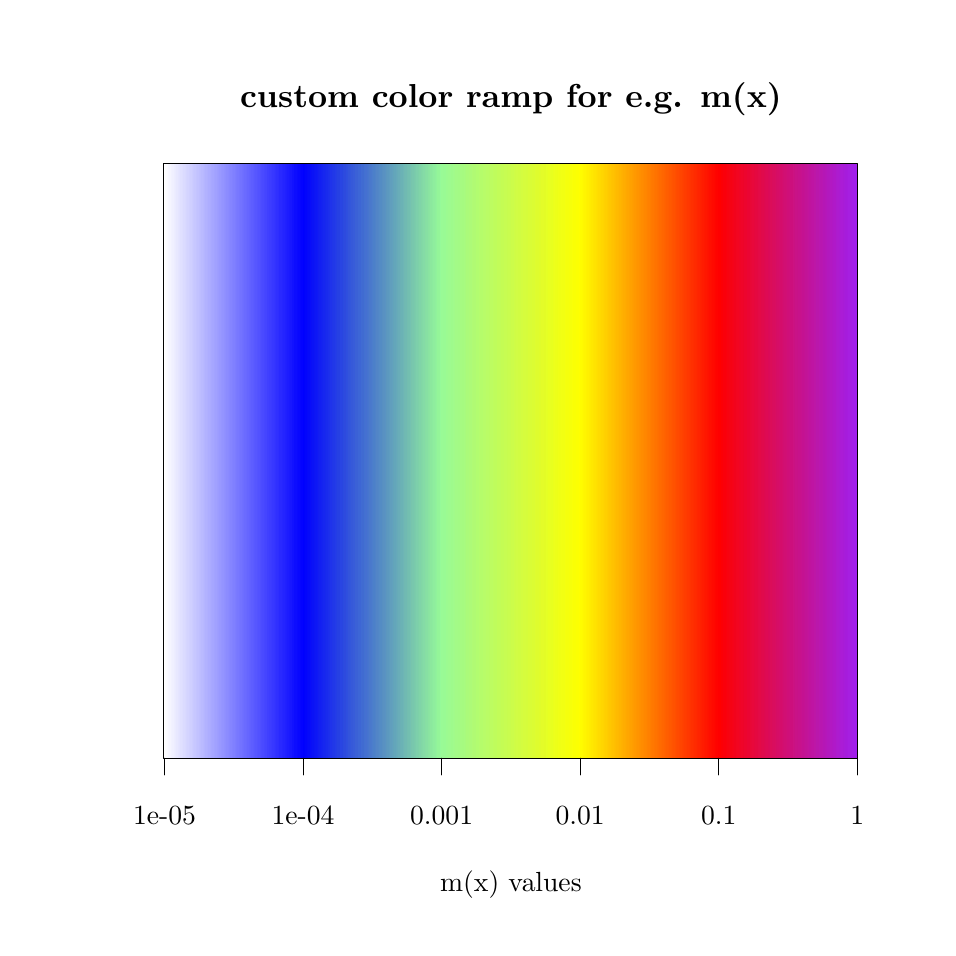
\begin{tikzpicture}[x=1pt,y=1pt]
\definecolor[named]{drawColor}{rgb}{0.00,0.00,0.00}
\definecolor[named]{fillColor}{rgb}{1.00,1.00,1.00}
\fill[color=fillColor,] (0,0) rectangle (325.21,325.21);
\begin{scope}
\path[clip] (  0.00,  0.00) rectangle (325.21,325.21);
\definecolor[named]{drawColor}{rgb}{0.24,0.00,0.33}
\definecolor[named]{drawColor}{rgb}{0.00,0.00,0.00}

\node[color=drawColor,anchor=base,inner sep=0pt, outer sep=0pt, scale=  1.20] at (174.61,296.47) {\bfseries custom color ramp for e.g. m(x)%
};

\node[color=drawColor,anchor=base,inner sep=0pt, outer sep=0pt, scale=  1.00] at (174.61, 13.20) {m(x) values%
};
\end{scope}
\begin{scope}
\path[clip] ( 49.20, 61.20) rectangle (300.01,276.01);
\definecolor[named]{drawColor}{rgb}{0.24,0.00,0.33}
\definecolor[named]{fillColor}{rgb}{1.00,1.00,1.00}

\draw[fill=fillColor,draw opacity=0.00,] ( 49.20, 61.20) rectangle ( 49.70,276.01);
\definecolor[named]{fillColor}{rgb}{0.99,0.99,1.00}

\draw[fill=fillColor,draw opacity=0.00,] ( 49.70, 61.20) rectangle ( 50.20,276.01);
\definecolor[named]{fillColor}{rgb}{0.98,0.98,1.00}

\draw[fill=fillColor,draw opacity=0.00,] ( 50.20, 61.20) rectangle ( 50.70,276.01);
\definecolor[named]{fillColor}{rgb}{0.97,0.97,1.00}

\draw[fill=fillColor,draw opacity=0.00,] ( 50.70, 61.20) rectangle ( 51.21,276.01);
\definecolor[named]{fillColor}{rgb}{0.96,0.96,1.00}

\draw[fill=fillColor,draw opacity=0.00,] ( 51.21, 61.20) rectangle ( 51.71,276.01);
\definecolor[named]{fillColor}{rgb}{0.95,0.95,1.00}

\draw[fill=fillColor,draw opacity=0.00,] ( 51.71, 61.20) rectangle ( 52.21,276.01);
\definecolor[named]{fillColor}{rgb}{0.94,0.94,1.00}

\draw[fill=fillColor,draw opacity=0.00,] ( 52.21, 61.20) rectangle ( 52.71,276.01);
\definecolor[named]{fillColor}{rgb}{0.93,0.93,1.00}

\draw[fill=fillColor,draw opacity=0.00,] ( 52.71, 61.20) rectangle ( 53.21,276.01);
\definecolor[named]{fillColor}{rgb}{0.92,0.92,1.00}

\draw[fill=fillColor,draw opacity=0.00,] ( 53.21, 61.20) rectangle ( 53.71,276.01);
\definecolor[named]{fillColor}{rgb}{0.91,0.91,1.00}

\draw[fill=fillColor,draw opacity=0.00,] ( 53.71, 61.20) rectangle ( 54.22,276.01);
\definecolor[named]{fillColor}{rgb}{0.90,0.90,1.00}

\draw[fill=fillColor,draw opacity=0.00,] ( 54.22, 61.20) rectangle ( 54.72,276.01);
\definecolor[named]{fillColor}{rgb}{0.89,0.89,1.00}

\draw[fill=fillColor,draw opacity=0.00,] ( 54.72, 61.20) rectangle ( 55.22,276.01);
\definecolor[named]{fillColor}{rgb}{0.88,0.88,1.00}

\draw[fill=fillColor,draw opacity=0.00,] ( 55.22, 61.20) rectangle ( 55.72,276.01);
\definecolor[named]{fillColor}{rgb}{0.87,0.87,1.00}

\draw[fill=fillColor,draw opacity=0.00,] ( 55.72, 61.20) rectangle ( 56.22,276.01);
\definecolor[named]{fillColor}{rgb}{0.86,0.86,1.00}

\draw[fill=fillColor,draw opacity=0.00,] ( 56.22, 61.20) rectangle ( 56.72,276.01);
\definecolor[named]{fillColor}{rgb}{0.85,0.85,1.00}

\draw[fill=fillColor,draw opacity=0.00,] ( 56.72, 61.20) rectangle ( 57.23,276.01);
\definecolor[named]{fillColor}{rgb}{0.84,0.84,1.00}

\draw[fill=fillColor,draw opacity=0.00,] ( 57.23, 61.20) rectangle ( 57.73,276.01);
\definecolor[named]{fillColor}{rgb}{0.83,0.83,1.00}

\draw[fill=fillColor,draw opacity=0.00,] ( 57.73, 61.20) rectangle ( 58.23,276.01);
\definecolor[named]{fillColor}{rgb}{0.82,0.82,1.00}

\draw[fill=fillColor,draw opacity=0.00,] ( 58.23, 61.20) rectangle ( 58.73,276.01);
\definecolor[named]{fillColor}{rgb}{0.81,0.81,1.00}

\draw[fill=fillColor,draw opacity=0.00,] ( 58.73, 61.20) rectangle ( 59.23,276.01);
\definecolor[named]{fillColor}{rgb}{0.80,0.80,1.00}

\draw[fill=fillColor,draw opacity=0.00,] ( 59.23, 61.20) rectangle ( 59.73,276.01);
\definecolor[named]{fillColor}{rgb}{0.79,0.79,1.00}

\draw[fill=fillColor,draw opacity=0.00,] ( 59.73, 61.20) rectangle ( 60.24,276.01);
\definecolor[named]{fillColor}{rgb}{0.78,0.78,1.00}

\draw[fill=fillColor,draw opacity=0.00,] ( 60.24, 61.20) rectangle ( 60.74,276.01);
\definecolor[named]{fillColor}{rgb}{0.77,0.77,1.00}

\draw[fill=fillColor,draw opacity=0.00,] ( 60.74, 61.20) rectangle ( 61.24,276.01);
\definecolor[named]{fillColor}{rgb}{0.76,0.76,1.00}

\draw[fill=fillColor,draw opacity=0.00,] ( 61.24, 61.20) rectangle ( 61.74,276.01);
\definecolor[named]{fillColor}{rgb}{0.75,0.75,1.00}

\draw[fill=fillColor,draw opacity=0.00,] ( 61.74, 61.20) rectangle ( 62.24,276.01);
\definecolor[named]{fillColor}{rgb}{0.74,0.74,1.00}

\draw[fill=fillColor,draw opacity=0.00,] ( 62.24, 61.20) rectangle ( 62.74,276.01);
\definecolor[named]{fillColor}{rgb}{0.73,0.73,1.00}

\draw[fill=fillColor,draw opacity=0.00,] ( 62.74, 61.20) rectangle ( 63.25,276.01);
\definecolor[named]{fillColor}{rgb}{0.72,0.72,1.00}

\draw[fill=fillColor,draw opacity=0.00,] ( 63.25, 61.20) rectangle ( 63.75,276.01);
\definecolor[named]{fillColor}{rgb}{0.71,0.71,1.00}

\draw[fill=fillColor,draw opacity=0.00,] ( 63.75, 61.20) rectangle ( 64.25,276.01);
\definecolor[named]{fillColor}{rgb}{0.70,0.70,1.00}

\draw[fill=fillColor,draw opacity=0.00,] ( 64.25, 61.20) rectangle ( 64.75,276.01);
\definecolor[named]{fillColor}{rgb}{0.69,0.69,1.00}

\draw[fill=fillColor,draw opacity=0.00,] ( 64.75, 61.20) rectangle ( 65.25,276.01);
\definecolor[named]{fillColor}{rgb}{0.68,0.68,1.00}

\draw[fill=fillColor,draw opacity=0.00,] ( 65.25, 61.20) rectangle ( 65.75,276.01);
\definecolor[named]{fillColor}{rgb}{0.67,0.67,1.00}

\draw[fill=fillColor,draw opacity=0.00,] ( 65.75, 61.20) rectangle ( 66.26,276.01);
\definecolor[named]{fillColor}{rgb}{0.66,0.66,1.00}

\draw[fill=fillColor,draw opacity=0.00,] ( 66.26, 61.20) rectangle ( 66.76,276.01);
\definecolor[named]{fillColor}{rgb}{0.65,0.65,1.00}

\draw[fill=fillColor,draw opacity=0.00,] ( 66.76, 61.20) rectangle ( 67.26,276.01);
\definecolor[named]{fillColor}{rgb}{0.64,0.64,1.00}

\draw[fill=fillColor,draw opacity=0.00,] ( 67.26, 61.20) rectangle ( 67.76,276.01);
\definecolor[named]{fillColor}{rgb}{0.63,0.63,1.00}

\draw[fill=fillColor,draw opacity=0.00,] ( 67.76, 61.20) rectangle ( 68.26,276.01);
\definecolor[named]{fillColor}{rgb}{0.62,0.62,1.00}

\draw[fill=fillColor,draw opacity=0.00,] ( 68.26, 61.20) rectangle ( 68.76,276.01);
\definecolor[named]{fillColor}{rgb}{0.61,0.61,1.00}

\draw[fill=fillColor,draw opacity=0.00,] ( 68.76, 61.20) rectangle ( 69.27,276.01);
\definecolor[named]{fillColor}{rgb}{0.60,0.60,1.00}

\draw[fill=fillColor,draw opacity=0.00,] ( 69.27, 61.20) rectangle ( 69.77,276.01);
\definecolor[named]{fillColor}{rgb}{0.59,0.59,1.00}

\draw[fill=fillColor,draw opacity=0.00,] ( 69.77, 61.20) rectangle ( 70.27,276.01);
\definecolor[named]{fillColor}{rgb}{0.58,0.58,1.00}

\draw[fill=fillColor,draw opacity=0.00,] ( 70.27, 61.20) rectangle ( 70.77,276.01);
\definecolor[named]{fillColor}{rgb}{0.57,0.57,1.00}

\draw[fill=fillColor,draw opacity=0.00,] ( 70.77, 61.20) rectangle ( 71.27,276.01);
\definecolor[named]{fillColor}{rgb}{0.56,0.56,1.00}

\draw[fill=fillColor,draw opacity=0.00,] ( 71.27, 61.20) rectangle ( 71.77,276.01);
\definecolor[named]{fillColor}{rgb}{0.55,0.55,1.00}

\draw[fill=fillColor,draw opacity=0.00,] ( 71.77, 61.20) rectangle ( 72.27,276.01);
\definecolor[named]{fillColor}{rgb}{0.54,0.54,1.00}

\draw[fill=fillColor,draw opacity=0.00,] ( 72.27, 61.20) rectangle ( 72.78,276.01);
\definecolor[named]{fillColor}{rgb}{0.53,0.53,1.00}

\draw[fill=fillColor,draw opacity=0.00,] ( 72.78, 61.20) rectangle ( 73.28,276.01);
\definecolor[named]{fillColor}{rgb}{0.52,0.52,1.00}

\draw[fill=fillColor,draw opacity=0.00,] ( 73.28, 61.20) rectangle ( 73.78,276.01);
\definecolor[named]{fillColor}{rgb}{0.51,0.51,1.00}

\draw[fill=fillColor,draw opacity=0.00,] ( 73.78, 61.20) rectangle ( 74.28,276.01);
\definecolor[named]{fillColor}{rgb}{0.50,0.50,1.00}

\draw[fill=fillColor,draw opacity=0.00,] ( 74.28, 61.20) rectangle ( 74.78,276.01);
\definecolor[named]{fillColor}{rgb}{0.49,0.49,1.00}

\draw[fill=fillColor,draw opacity=0.00,] ( 74.78, 61.20) rectangle ( 75.28,276.01);
\definecolor[named]{fillColor}{rgb}{0.48,0.48,1.00}

\draw[fill=fillColor,draw opacity=0.00,] ( 75.28, 61.20) rectangle ( 75.79,276.01);
\definecolor[named]{fillColor}{rgb}{0.47,0.47,1.00}

\draw[fill=fillColor,draw opacity=0.00,] ( 75.79, 61.20) rectangle ( 76.29,276.01);
\definecolor[named]{fillColor}{rgb}{0.46,0.46,1.00}

\draw[fill=fillColor,draw opacity=0.00,] ( 76.29, 61.20) rectangle ( 76.79,276.01);
\definecolor[named]{fillColor}{rgb}{0.45,0.45,1.00}

\draw[fill=fillColor,draw opacity=0.00,] ( 76.79, 61.20) rectangle ( 77.29,276.01);
\definecolor[named]{fillColor}{rgb}{0.44,0.44,1.00}

\draw[fill=fillColor,draw opacity=0.00,] ( 77.29, 61.20) rectangle ( 77.79,276.01);
\definecolor[named]{fillColor}{rgb}{0.43,0.43,1.00}

\draw[fill=fillColor,draw opacity=0.00,] ( 77.79, 61.20) rectangle ( 78.29,276.01);
\definecolor[named]{fillColor}{rgb}{0.42,0.42,1.00}

\draw[fill=fillColor,draw opacity=0.00,] ( 78.29, 61.20) rectangle ( 78.80,276.01);
\definecolor[named]{fillColor}{rgb}{0.41,0.41,1.00}

\draw[fill=fillColor,draw opacity=0.00,] ( 78.80, 61.20) rectangle ( 79.30,276.01);
\definecolor[named]{fillColor}{rgb}{0.40,0.40,1.00}

\draw[fill=fillColor,draw opacity=0.00,] ( 79.30, 61.20) rectangle ( 79.80,276.01);
\definecolor[named]{fillColor}{rgb}{0.39,0.39,1.00}

\draw[fill=fillColor,draw opacity=0.00,] ( 79.80, 61.20) rectangle ( 80.30,276.01);
\definecolor[named]{fillColor}{rgb}{0.38,0.38,1.00}

\draw[fill=fillColor,draw opacity=0.00,] ( 80.30, 61.20) rectangle ( 80.80,276.01);
\definecolor[named]{fillColor}{rgb}{0.37,0.37,1.00}

\draw[fill=fillColor,draw opacity=0.00,] ( 80.80, 61.20) rectangle ( 81.30,276.01);
\definecolor[named]{fillColor}{rgb}{0.36,0.36,1.00}

\draw[fill=fillColor,draw opacity=0.00,] ( 81.30, 61.20) rectangle ( 81.81,276.01);
\definecolor[named]{fillColor}{rgb}{0.35,0.35,1.00}

\draw[fill=fillColor,draw opacity=0.00,] ( 81.81, 61.20) rectangle ( 82.31,276.01);
\definecolor[named]{fillColor}{rgb}{0.34,0.34,1.00}

\draw[fill=fillColor,draw opacity=0.00,] ( 82.31, 61.20) rectangle ( 82.81,276.01);
\definecolor[named]{fillColor}{rgb}{0.33,0.33,1.00}

\draw[fill=fillColor,draw opacity=0.00,] ( 82.81, 61.20) rectangle ( 83.31,276.01);
\definecolor[named]{fillColor}{rgb}{0.32,0.32,1.00}

\draw[fill=fillColor,draw opacity=0.00,] ( 83.31, 61.20) rectangle ( 83.81,276.01);
\definecolor[named]{fillColor}{rgb}{0.31,0.31,1.00}

\draw[fill=fillColor,draw opacity=0.00,] ( 83.81, 61.20) rectangle ( 84.31,276.01);
\definecolor[named]{fillColor}{rgb}{0.30,0.30,1.00}

\draw[fill=fillColor,draw opacity=0.00,] ( 84.31, 61.20) rectangle ( 84.82,276.01);
\definecolor[named]{fillColor}{rgb}{0.29,0.29,1.00}

\draw[fill=fillColor,draw opacity=0.00,] ( 84.82, 61.20) rectangle ( 85.32,276.01);
\definecolor[named]{fillColor}{rgb}{0.28,0.28,1.00}

\draw[fill=fillColor,draw opacity=0.00,] ( 85.32, 61.20) rectangle ( 85.82,276.01);
\definecolor[named]{fillColor}{rgb}{0.27,0.27,1.00}

\draw[fill=fillColor,draw opacity=0.00,] ( 85.82, 61.20) rectangle ( 86.32,276.01);
\definecolor[named]{fillColor}{rgb}{0.25,0.25,1.00}

\draw[fill=fillColor,draw opacity=0.00,] ( 86.32, 61.20) rectangle ( 86.82,276.01);
\definecolor[named]{fillColor}{rgb}{0.25,0.25,1.00}

\draw[fill=fillColor,draw opacity=0.00,] ( 86.82, 61.20) rectangle ( 87.32,276.01);
\definecolor[named]{fillColor}{rgb}{0.24,0.24,1.00}

\draw[fill=fillColor,draw opacity=0.00,] ( 87.32, 61.20) rectangle ( 87.83,276.01);
\definecolor[named]{fillColor}{rgb}{0.23,0.23,1.00}

\draw[fill=fillColor,draw opacity=0.00,] ( 87.83, 61.20) rectangle ( 88.33,276.01);
\definecolor[named]{fillColor}{rgb}{0.22,0.22,1.00}

\draw[fill=fillColor,draw opacity=0.00,] ( 88.33, 61.20) rectangle ( 88.83,276.01);
\definecolor[named]{fillColor}{rgb}{0.21,0.21,1.00}

\draw[fill=fillColor,draw opacity=0.00,] ( 88.83, 61.20) rectangle ( 89.33,276.01);
\definecolor[named]{fillColor}{rgb}{0.20,0.20,1.00}

\draw[fill=fillColor,draw opacity=0.00,] ( 89.33, 61.20) rectangle ( 89.83,276.01);
\definecolor[named]{fillColor}{rgb}{0.19,0.19,1.00}

\draw[fill=fillColor,draw opacity=0.00,] ( 89.83, 61.20) rectangle ( 90.33,276.01);
\definecolor[named]{fillColor}{rgb}{0.18,0.18,1.00}

\draw[fill=fillColor,draw opacity=0.00,] ( 90.33, 61.20) rectangle ( 90.84,276.01);
\definecolor[named]{fillColor}{rgb}{0.16,0.16,1.00}

\draw[fill=fillColor,draw opacity=0.00,] ( 90.84, 61.20) rectangle ( 91.34,276.01);
\definecolor[named]{fillColor}{rgb}{0.16,0.16,1.00}

\draw[fill=fillColor,draw opacity=0.00,] ( 91.34, 61.20) rectangle ( 91.84,276.01);
\definecolor[named]{fillColor}{rgb}{0.15,0.15,1.00}

\draw[fill=fillColor,draw opacity=0.00,] ( 91.84, 61.20) rectangle ( 92.34,276.01);
\definecolor[named]{fillColor}{rgb}{0.14,0.14,1.00}

\draw[fill=fillColor,draw opacity=0.00,] ( 92.34, 61.20) rectangle ( 92.84,276.01);
\definecolor[named]{fillColor}{rgb}{0.13,0.13,1.00}

\draw[fill=fillColor,draw opacity=0.00,] ( 92.84, 61.20) rectangle ( 93.34,276.01);
\definecolor[named]{fillColor}{rgb}{0.12,0.12,1.00}

\draw[fill=fillColor,draw opacity=0.00,] ( 93.34, 61.20) rectangle ( 93.85,276.01);
\definecolor[named]{fillColor}{rgb}{0.11,0.11,1.00}

\draw[fill=fillColor,draw opacity=0.00,] ( 93.85, 61.20) rectangle ( 94.35,276.01);
\definecolor[named]{fillColor}{rgb}{0.10,0.10,1.00}

\draw[fill=fillColor,draw opacity=0.00,] ( 94.35, 61.20) rectangle ( 94.85,276.01);
\definecolor[named]{fillColor}{rgb}{0.09,0.09,1.00}

\draw[fill=fillColor,draw opacity=0.00,] ( 94.85, 61.20) rectangle ( 95.35,276.01);
\definecolor[named]{fillColor}{rgb}{0.07,0.07,1.00}

\draw[fill=fillColor,draw opacity=0.00,] ( 95.35, 61.20) rectangle ( 95.85,276.01);
\definecolor[named]{fillColor}{rgb}{0.07,0.07,1.00}

\draw[fill=fillColor,draw opacity=0.00,] ( 95.85, 61.20) rectangle ( 96.35,276.01);
\definecolor[named]{fillColor}{rgb}{0.05,0.05,1.00}

\draw[fill=fillColor,draw opacity=0.00,] ( 96.35, 61.20) rectangle ( 96.85,276.01);
\definecolor[named]{fillColor}{rgb}{0.05,0.05,1.00}

\draw[fill=fillColor,draw opacity=0.00,] ( 96.85, 61.20) rectangle ( 97.36,276.01);
\definecolor[named]{fillColor}{rgb}{0.04,0.04,1.00}

\draw[fill=fillColor,draw opacity=0.00,] ( 97.36, 61.20) rectangle ( 97.86,276.01);
\definecolor[named]{fillColor}{rgb}{0.03,0.03,1.00}

\draw[fill=fillColor,draw opacity=0.00,] ( 97.86, 61.20) rectangle ( 98.36,276.01);
\definecolor[named]{fillColor}{rgb}{0.02,0.02,1.00}

\draw[fill=fillColor,draw opacity=0.00,] ( 98.36, 61.20) rectangle ( 98.86,276.01);
\definecolor[named]{fillColor}{rgb}{0.01,0.01,1.00}

\draw[fill=fillColor,draw opacity=0.00,] ( 98.86, 61.20) rectangle ( 99.36,276.01);
\definecolor[named]{fillColor}{rgb}{0.00,0.00,1.00}

\draw[fill=fillColor,draw opacity=0.00,] ( 99.36, 61.20) rectangle ( 99.86,276.01);
\definecolor[named]{fillColor}{rgb}{0.00,0.01,0.99}

\draw[fill=fillColor,draw opacity=0.00,] ( 99.86, 61.20) rectangle (100.37,276.01);
\definecolor[named]{fillColor}{rgb}{0.01,0.02,0.99}

\draw[fill=fillColor,draw opacity=0.00,] (100.37, 61.20) rectangle (100.87,276.01);
\definecolor[named]{fillColor}{rgb}{0.02,0.03,0.98}

\draw[fill=fillColor,draw opacity=0.00,] (100.87, 61.20) rectangle (101.37,276.01);
\definecolor[named]{fillColor}{rgb}{0.02,0.04,0.98}

\draw[fill=fillColor,draw opacity=0.00,] (101.37, 61.20) rectangle (101.87,276.01);
\definecolor[named]{fillColor}{rgb}{0.03,0.05,0.98}

\draw[fill=fillColor,draw opacity=0.00,] (101.87, 61.20) rectangle (102.37,276.01);
\definecolor[named]{fillColor}{rgb}{0.04,0.06,0.97}

\draw[fill=fillColor,draw opacity=0.00,] (102.37, 61.20) rectangle (102.87,276.01);
\definecolor[named]{fillColor}{rgb}{0.04,0.07,0.97}

\draw[fill=fillColor,draw opacity=0.00,] (102.87, 61.20) rectangle (103.38,276.01);
\definecolor[named]{fillColor}{rgb}{0.05,0.08,0.96}

\draw[fill=fillColor,draw opacity=0.00,] (103.38, 61.20) rectangle (103.88,276.01);
\definecolor[named]{fillColor}{rgb}{0.05,0.09,0.96}

\draw[fill=fillColor,draw opacity=0.00,] (103.88, 61.20) rectangle (104.38,276.01);
\definecolor[named]{fillColor}{rgb}{0.06,0.10,0.96}

\draw[fill=fillColor,draw opacity=0.00,] (104.38, 61.20) rectangle (104.88,276.01);
\definecolor[named]{fillColor}{rgb}{0.07,0.11,0.95}

\draw[fill=fillColor,draw opacity=0.00,] (104.88, 61.20) rectangle (105.38,276.01);
\definecolor[named]{fillColor}{rgb}{0.07,0.12,0.95}

\draw[fill=fillColor,draw opacity=0.00,] (105.38, 61.20) rectangle (105.88,276.01);
\definecolor[named]{fillColor}{rgb}{0.08,0.13,0.95}

\draw[fill=fillColor,draw opacity=0.00,] (105.88, 61.20) rectangle (106.39,276.01);
\definecolor[named]{fillColor}{rgb}{0.08,0.14,0.94}

\draw[fill=fillColor,draw opacity=0.00,] (106.39, 61.20) rectangle (106.89,276.01);
\definecolor[named]{fillColor}{rgb}{0.09,0.15,0.94}

\draw[fill=fillColor,draw opacity=0.00,] (106.89, 61.20) rectangle (107.39,276.01);
\definecolor[named]{fillColor}{rgb}{0.09,0.16,0.93}

\draw[fill=fillColor,draw opacity=0.00,] (107.39, 61.20) rectangle (107.89,276.01);
\definecolor[named]{fillColor}{rgb}{0.10,0.17,0.93}

\draw[fill=fillColor,draw opacity=0.00,] (107.89, 61.20) rectangle (108.39,276.01);
\definecolor[named]{fillColor}{rgb}{0.11,0.18,0.93}

\draw[fill=fillColor,draw opacity=0.00,] (108.39, 61.20) rectangle (108.89,276.01);
\definecolor[named]{fillColor}{rgb}{0.11,0.19,0.92}

\draw[fill=fillColor,draw opacity=0.00,] (108.89, 61.20) rectangle (109.40,276.01);
\definecolor[named]{fillColor}{rgb}{0.12,0.20,0.92}

\draw[fill=fillColor,draw opacity=0.00,] (109.40, 61.20) rectangle (109.90,276.01);
\definecolor[named]{fillColor}{rgb}{0.13,0.21,0.91}

\draw[fill=fillColor,draw opacity=0.00,] (109.90, 61.20) rectangle (110.40,276.01);
\definecolor[named]{fillColor}{rgb}{0.13,0.22,0.91}

\draw[fill=fillColor,draw opacity=0.00,] (110.40, 61.20) rectangle (110.90,276.01);
\definecolor[named]{fillColor}{rgb}{0.14,0.23,0.91}

\draw[fill=fillColor,draw opacity=0.00,] (110.90, 61.20) rectangle (111.40,276.01);
\definecolor[named]{fillColor}{rgb}{0.14,0.24,0.90}

\draw[fill=fillColor,draw opacity=0.00,] (111.40, 61.20) rectangle (111.90,276.01);
\definecolor[named]{fillColor}{rgb}{0.15,0.25,0.89}

\draw[fill=fillColor,draw opacity=0.00,] (111.90, 61.20) rectangle (112.41,276.01);
\definecolor[named]{fillColor}{rgb}{0.15,0.25,0.89}

\draw[fill=fillColor,draw opacity=0.00,] (112.41, 61.20) rectangle (112.91,276.01);
\definecolor[named]{fillColor}{rgb}{0.16,0.27,0.89}

\draw[fill=fillColor,draw opacity=0.00,] (112.91, 61.20) rectangle (113.41,276.01);
\definecolor[named]{fillColor}{rgb}{0.16,0.27,0.88}

\draw[fill=fillColor,draw opacity=0.00,] (113.41, 61.20) rectangle (113.91,276.01);
\definecolor[named]{fillColor}{rgb}{0.17,0.29,0.88}

\draw[fill=fillColor,draw opacity=0.00,] (113.91, 61.20) rectangle (114.41,276.01);
\definecolor[named]{fillColor}{rgb}{0.18,0.29,0.87}

\draw[fill=fillColor,draw opacity=0.00,] (114.41, 61.20) rectangle (114.91,276.01);
\definecolor[named]{fillColor}{rgb}{0.18,0.31,0.87}

\draw[fill=fillColor,draw opacity=0.00,] (114.91, 61.20) rectangle (115.42,276.01);
\definecolor[named]{fillColor}{rgb}{0.19,0.31,0.87}

\draw[fill=fillColor,draw opacity=0.00,] (115.42, 61.20) rectangle (115.92,276.01);
\definecolor[named]{fillColor}{rgb}{0.20,0.33,0.86}

\draw[fill=fillColor,draw opacity=0.00,] (115.92, 61.20) rectangle (116.42,276.01);
\definecolor[named]{fillColor}{rgb}{0.20,0.34,0.86}

\draw[fill=fillColor,draw opacity=0.00,] (116.42, 61.20) rectangle (116.92,276.01);
\definecolor[named]{fillColor}{rgb}{0.21,0.35,0.85}

\draw[fill=fillColor,draw opacity=0.00,] (116.92, 61.20) rectangle (117.42,276.01);
\definecolor[named]{fillColor}{rgb}{0.22,0.36,0.85}

\draw[fill=fillColor,draw opacity=0.00,] (117.42, 61.20) rectangle (117.92,276.01);
\definecolor[named]{fillColor}{rgb}{0.22,0.36,0.85}

\draw[fill=fillColor,draw opacity=0.00,] (117.92, 61.20) rectangle (118.42,276.01);
\definecolor[named]{fillColor}{rgb}{0.23,0.38,0.84}

\draw[fill=fillColor,draw opacity=0.00,] (118.42, 61.20) rectangle (118.93,276.01);
\definecolor[named]{fillColor}{rgb}{0.23,0.38,0.84}

\draw[fill=fillColor,draw opacity=0.00,] (118.93, 61.20) rectangle (119.43,276.01);
\definecolor[named]{fillColor}{rgb}{0.24,0.40,0.84}

\draw[fill=fillColor,draw opacity=0.00,] (119.43, 61.20) rectangle (119.93,276.01);
\definecolor[named]{fillColor}{rgb}{0.24,0.40,0.83}

\draw[fill=fillColor,draw opacity=0.00,] (119.93, 61.20) rectangle (120.43,276.01);
\definecolor[named]{fillColor}{rgb}{0.25,0.42,0.83}

\draw[fill=fillColor,draw opacity=0.00,] (120.43, 61.20) rectangle (120.93,276.01);
\definecolor[named]{fillColor}{rgb}{0.25,0.42,0.82}

\draw[fill=fillColor,draw opacity=0.00,] (120.93, 61.20) rectangle (121.43,276.01);
\definecolor[named]{fillColor}{rgb}{0.26,0.44,0.82}

\draw[fill=fillColor,draw opacity=0.00,] (121.43, 61.20) rectangle (121.94,276.01);
\definecolor[named]{fillColor}{rgb}{0.27,0.44,0.82}

\draw[fill=fillColor,draw opacity=0.00,] (121.94, 61.20) rectangle (122.44,276.01);
\definecolor[named]{fillColor}{rgb}{0.27,0.45,0.81}

\draw[fill=fillColor,draw opacity=0.00,] (122.44, 61.20) rectangle (122.94,276.01);
\definecolor[named]{fillColor}{rgb}{0.28,0.46,0.81}

\draw[fill=fillColor,draw opacity=0.00,] (122.94, 61.20) rectangle (123.44,276.01);
\definecolor[named]{fillColor}{rgb}{0.29,0.47,0.80}

\draw[fill=fillColor,draw opacity=0.00,] (123.44, 61.20) rectangle (123.94,276.01);
\definecolor[named]{fillColor}{rgb}{0.29,0.48,0.80}

\draw[fill=fillColor,draw opacity=0.00,] (123.94, 61.20) rectangle (124.44,276.01);
\definecolor[named]{fillColor}{rgb}{0.30,0.49,0.80}

\draw[fill=fillColor,draw opacity=0.00,] (124.44, 61.20) rectangle (124.95,276.01);
\definecolor[named]{fillColor}{rgb}{0.30,0.50,0.79}

\draw[fill=fillColor,draw opacity=0.00,] (124.95, 61.20) rectangle (125.45,276.01);
\definecolor[named]{fillColor}{rgb}{0.31,0.51,0.79}

\draw[fill=fillColor,draw opacity=0.00,] (125.45, 61.20) rectangle (125.95,276.01);
\definecolor[named]{fillColor}{rgb}{0.32,0.52,0.78}

\draw[fill=fillColor,draw opacity=0.00,] (125.95, 61.20) rectangle (126.45,276.01);
\definecolor[named]{fillColor}{rgb}{0.32,0.53,0.78}

\draw[fill=fillColor,draw opacity=0.00,] (126.45, 61.20) rectangle (126.95,276.01);
\definecolor[named]{fillColor}{rgb}{0.33,0.54,0.78}

\draw[fill=fillColor,draw opacity=0.00,] (126.95, 61.20) rectangle (127.45,276.01);
\definecolor[named]{fillColor}{rgb}{0.33,0.55,0.77}

\draw[fill=fillColor,draw opacity=0.00,] (127.45, 61.20) rectangle (127.96,276.01);
\definecolor[named]{fillColor}{rgb}{0.34,0.56,0.76}

\draw[fill=fillColor,draw opacity=0.00,] (127.96, 61.20) rectangle (128.46,276.01);
\definecolor[named]{fillColor}{rgb}{0.35,0.57,0.76}

\draw[fill=fillColor,draw opacity=0.00,] (128.46, 61.20) rectangle (128.96,276.01);
\definecolor[named]{fillColor}{rgb}{0.35,0.58,0.76}

\draw[fill=fillColor,draw opacity=0.00,] (128.96, 61.20) rectangle (129.46,276.01);
\definecolor[named]{fillColor}{rgb}{0.36,0.59,0.75}

\draw[fill=fillColor,draw opacity=0.00,] (129.46, 61.20) rectangle (129.96,276.01);
\definecolor[named]{fillColor}{rgb}{0.36,0.60,0.75}

\draw[fill=fillColor,draw opacity=0.00,] (129.96, 61.20) rectangle (130.46,276.01);
\definecolor[named]{fillColor}{rgb}{0.37,0.61,0.75}

\draw[fill=fillColor,draw opacity=0.00,] (130.46, 61.20) rectangle (130.97,276.01);
\definecolor[named]{fillColor}{rgb}{0.38,0.62,0.74}

\draw[fill=fillColor,draw opacity=0.00,] (130.97, 61.20) rectangle (131.47,276.01);
\definecolor[named]{fillColor}{rgb}{0.38,0.63,0.74}

\draw[fill=fillColor,draw opacity=0.00,] (131.47, 61.20) rectangle (131.97,276.01);
\definecolor[named]{fillColor}{rgb}{0.39,0.64,0.73}

\draw[fill=fillColor,draw opacity=0.00,] (131.97, 61.20) rectangle (132.47,276.01);
\definecolor[named]{fillColor}{rgb}{0.39,0.65,0.73}

\draw[fill=fillColor,draw opacity=0.00,] (132.47, 61.20) rectangle (132.97,276.01);
\definecolor[named]{fillColor}{rgb}{0.40,0.66,0.73}

\draw[fill=fillColor,draw opacity=0.00,] (132.97, 61.20) rectangle (133.47,276.01);
\definecolor[named]{fillColor}{rgb}{0.40,0.67,0.72}

\draw[fill=fillColor,draw opacity=0.00,] (133.47, 61.20) rectangle (133.98,276.01);
\definecolor[named]{fillColor}{rgb}{0.41,0.68,0.72}

\draw[fill=fillColor,draw opacity=0.00,] (133.98, 61.20) rectangle (134.48,276.01);
\definecolor[named]{fillColor}{rgb}{0.42,0.69,0.71}

\draw[fill=fillColor,draw opacity=0.00,] (134.48, 61.20) rectangle (134.98,276.01);
\definecolor[named]{fillColor}{rgb}{0.42,0.70,0.71}

\draw[fill=fillColor,draw opacity=0.00,] (134.98, 61.20) rectangle (135.48,276.01);
\definecolor[named]{fillColor}{rgb}{0.43,0.71,0.71}

\draw[fill=fillColor,draw opacity=0.00,] (135.48, 61.20) rectangle (135.98,276.01);
\definecolor[named]{fillColor}{rgb}{0.44,0.72,0.70}

\draw[fill=fillColor,draw opacity=0.00,] (135.98, 61.20) rectangle (136.48,276.01);
\definecolor[named]{fillColor}{rgb}{0.44,0.73,0.70}

\draw[fill=fillColor,draw opacity=0.00,] (136.48, 61.20) rectangle (136.99,276.01);
\definecolor[named]{fillColor}{rgb}{0.45,0.74,0.69}

\draw[fill=fillColor,draw opacity=0.00,] (136.99, 61.20) rectangle (137.49,276.01);
\definecolor[named]{fillColor}{rgb}{0.45,0.75,0.69}

\draw[fill=fillColor,draw opacity=0.00,] (137.49, 61.20) rectangle (137.99,276.01);
\definecolor[named]{fillColor}{rgb}{0.46,0.76,0.69}

\draw[fill=fillColor,draw opacity=0.00,] (137.99, 61.20) rectangle (138.49,276.01);
\definecolor[named]{fillColor}{rgb}{0.47,0.77,0.68}

\draw[fill=fillColor,draw opacity=0.00,] (138.49, 61.20) rectangle (138.99,276.01);
\definecolor[named]{fillColor}{rgb}{0.47,0.78,0.68}

\draw[fill=fillColor,draw opacity=0.00,] (138.99, 61.20) rectangle (139.49,276.01);
\definecolor[named]{fillColor}{rgb}{0.48,0.79,0.67}

\draw[fill=fillColor,draw opacity=0.00,] (139.49, 61.20) rectangle (140.00,276.01);
\definecolor[named]{fillColor}{rgb}{0.48,0.80,0.67}

\draw[fill=fillColor,draw opacity=0.00,] (140.00, 61.20) rectangle (140.50,276.01);
\definecolor[named]{fillColor}{rgb}{0.49,0.81,0.67}

\draw[fill=fillColor,draw opacity=0.00,] (140.50, 61.20) rectangle (141.00,276.01);
\definecolor[named]{fillColor}{rgb}{0.49,0.82,0.66}

\draw[fill=fillColor,draw opacity=0.00,] (141.00, 61.20) rectangle (141.50,276.01);
\definecolor[named]{fillColor}{rgb}{0.50,0.83,0.66}

\draw[fill=fillColor,draw opacity=0.00,] (141.50, 61.20) rectangle (142.00,276.01);
\definecolor[named]{fillColor}{rgb}{0.51,0.84,0.65}

\draw[fill=fillColor,draw opacity=0.00,] (142.00, 61.20) rectangle (142.50,276.01);
\definecolor[named]{fillColor}{rgb}{0.51,0.85,0.65}

\draw[fill=fillColor,draw opacity=0.00,] (142.50, 61.20) rectangle (143.00,276.01);
\definecolor[named]{fillColor}{rgb}{0.52,0.86,0.65}

\draw[fill=fillColor,draw opacity=0.00,] (143.00, 61.20) rectangle (143.51,276.01);
\definecolor[named]{fillColor}{rgb}{0.53,0.87,0.64}

\draw[fill=fillColor,draw opacity=0.00,] (143.51, 61.20) rectangle (144.01,276.01);
\definecolor[named]{fillColor}{rgb}{0.53,0.88,0.64}

\draw[fill=fillColor,draw opacity=0.00,] (144.01, 61.20) rectangle (144.51,276.01);
\definecolor[named]{fillColor}{rgb}{0.54,0.89,0.63}

\draw[fill=fillColor,draw opacity=0.00,] (144.51, 61.20) rectangle (145.01,276.01);
\definecolor[named]{fillColor}{rgb}{0.54,0.90,0.63}

\draw[fill=fillColor,draw opacity=0.00,] (145.01, 61.20) rectangle (145.51,276.01);
\definecolor[named]{fillColor}{rgb}{0.55,0.91,0.62}

\draw[fill=fillColor,draw opacity=0.00,] (145.51, 61.20) rectangle (146.01,276.01);
\definecolor[named]{fillColor}{rgb}{0.55,0.92,0.62}

\draw[fill=fillColor,draw opacity=0.00,] (146.01, 61.20) rectangle (146.52,276.01);
\definecolor[named]{fillColor}{rgb}{0.56,0.93,0.62}

\draw[fill=fillColor,draw opacity=0.00,] (146.52, 61.20) rectangle (147.02,276.01);
\definecolor[named]{fillColor}{rgb}{0.56,0.94,0.61}

\draw[fill=fillColor,draw opacity=0.00,] (147.02, 61.20) rectangle (147.52,276.01);
\definecolor[named]{fillColor}{rgb}{0.57,0.95,0.61}

\draw[fill=fillColor,draw opacity=0.00,] (147.52, 61.20) rectangle (148.02,276.01);
\definecolor[named]{fillColor}{rgb}{0.58,0.96,0.60}

\draw[fill=fillColor,draw opacity=0.00,] (148.02, 61.20) rectangle (148.52,276.01);
\definecolor[named]{fillColor}{rgb}{0.58,0.96,0.60}

\draw[fill=fillColor,draw opacity=0.00,] (148.52, 61.20) rectangle (149.02,276.01);
\definecolor[named]{fillColor}{rgb}{0.59,0.98,0.60}

\draw[fill=fillColor,draw opacity=0.00,] (149.02, 61.20) rectangle (149.53,276.01);
\definecolor[named]{fillColor}{rgb}{0.60,0.98,0.59}

\draw[fill=fillColor,draw opacity=0.00,] (149.53, 61.20) rectangle (150.03,276.01);
\definecolor[named]{fillColor}{rgb}{0.60,0.98,0.58}

\draw[fill=fillColor,draw opacity=0.00,] (150.03, 61.20) rectangle (150.53,276.01);
\definecolor[named]{fillColor}{rgb}{0.60,0.98,0.58}

\draw[fill=fillColor,draw opacity=0.00,] (150.53, 61.20) rectangle (151.03,276.01);
\definecolor[named]{fillColor}{rgb}{0.61,0.98,0.57}

\draw[fill=fillColor,draw opacity=0.00,] (151.03, 61.20) rectangle (151.53,276.01);
\definecolor[named]{fillColor}{rgb}{0.61,0.98,0.57}

\draw[fill=fillColor,draw opacity=0.00,] (151.53, 61.20) rectangle (152.03,276.01);
\definecolor[named]{fillColor}{rgb}{0.62,0.98,0.56}

\draw[fill=fillColor,draw opacity=0.00,] (152.03, 61.20) rectangle (152.54,276.01);
\definecolor[named]{fillColor}{rgb}{0.62,0.98,0.56}

\draw[fill=fillColor,draw opacity=0.00,] (152.54, 61.20) rectangle (153.04,276.01);
\definecolor[named]{fillColor}{rgb}{0.62,0.98,0.55}

\draw[fill=fillColor,draw opacity=0.00,] (153.04, 61.20) rectangle (153.54,276.01);
\definecolor[named]{fillColor}{rgb}{0.63,0.98,0.55}

\draw[fill=fillColor,draw opacity=0.00,] (153.54, 61.20) rectangle (154.04,276.01);
\definecolor[named]{fillColor}{rgb}{0.63,0.98,0.54}

\draw[fill=fillColor,draw opacity=0.00,] (154.04, 61.20) rectangle (154.54,276.01);
\definecolor[named]{fillColor}{rgb}{0.64,0.98,0.53}

\draw[fill=fillColor,draw opacity=0.00,] (154.54, 61.20) rectangle (155.04,276.01);
\definecolor[named]{fillColor}{rgb}{0.64,0.98,0.53}

\draw[fill=fillColor,draw opacity=0.00,] (155.04, 61.20) rectangle (155.55,276.01);
\definecolor[named]{fillColor}{rgb}{0.64,0.98,0.52}

\draw[fill=fillColor,draw opacity=0.00,] (155.55, 61.20) rectangle (156.05,276.01);
\definecolor[named]{fillColor}{rgb}{0.65,0.98,0.51}

\draw[fill=fillColor,draw opacity=0.00,] (156.05, 61.20) rectangle (156.55,276.01);
\definecolor[named]{fillColor}{rgb}{0.65,0.98,0.51}

\draw[fill=fillColor,draw opacity=0.00,] (156.55, 61.20) rectangle (157.05,276.01);
\definecolor[named]{fillColor}{rgb}{0.65,0.98,0.50}

\draw[fill=fillColor,draw opacity=0.00,] (157.05, 61.20) rectangle (157.55,276.01);
\definecolor[named]{fillColor}{rgb}{0.66,0.98,0.50}

\draw[fill=fillColor,draw opacity=0.00,] (157.55, 61.20) rectangle (158.05,276.01);
\definecolor[named]{fillColor}{rgb}{0.66,0.98,0.49}

\draw[fill=fillColor,draw opacity=0.00,] (158.05, 61.20) rectangle (158.56,276.01);
\definecolor[named]{fillColor}{rgb}{0.67,0.98,0.48}

\draw[fill=fillColor,draw opacity=0.00,] (158.56, 61.20) rectangle (159.06,276.01);
\definecolor[named]{fillColor}{rgb}{0.67,0.98,0.48}

\draw[fill=fillColor,draw opacity=0.00,] (159.06, 61.20) rectangle (159.56,276.01);
\definecolor[named]{fillColor}{rgb}{0.68,0.98,0.47}

\draw[fill=fillColor,draw opacity=0.00,] (159.56, 61.20) rectangle (160.06,276.01);
\definecolor[named]{fillColor}{rgb}{0.68,0.98,0.47}

\draw[fill=fillColor,draw opacity=0.00,] (160.06, 61.20) rectangle (160.56,276.01);
\definecolor[named]{fillColor}{rgb}{0.69,0.98,0.46}

\draw[fill=fillColor,draw opacity=0.00,] (160.56, 61.20) rectangle (161.06,276.01);
\definecolor[named]{fillColor}{rgb}{0.69,0.98,0.45}

\draw[fill=fillColor,draw opacity=0.00,] (161.06, 61.20) rectangle (161.57,276.01);
\definecolor[named]{fillColor}{rgb}{0.69,0.98,0.45}

\draw[fill=fillColor,draw opacity=0.00,] (161.57, 61.20) rectangle (162.07,276.01);
\definecolor[named]{fillColor}{rgb}{0.70,0.99,0.44}

\draw[fill=fillColor,draw opacity=0.00,] (162.07, 61.20) rectangle (162.57,276.01);
\definecolor[named]{fillColor}{rgb}{0.70,0.99,0.44}

\draw[fill=fillColor,draw opacity=0.00,] (162.57, 61.20) rectangle (163.07,276.01);
\definecolor[named]{fillColor}{rgb}{0.71,0.99,0.43}

\draw[fill=fillColor,draw opacity=0.00,] (163.07, 61.20) rectangle (163.57,276.01);
\definecolor[named]{fillColor}{rgb}{0.71,0.99,0.42}

\draw[fill=fillColor,draw opacity=0.00,] (163.57, 61.20) rectangle (164.07,276.01);
\definecolor[named]{fillColor}{rgb}{0.71,0.99,0.42}

\draw[fill=fillColor,draw opacity=0.00,] (164.07, 61.20) rectangle (164.57,276.01);
\definecolor[named]{fillColor}{rgb}{0.72,0.99,0.41}

\draw[fill=fillColor,draw opacity=0.00,] (164.57, 61.20) rectangle (165.08,276.01);
\definecolor[named]{fillColor}{rgb}{0.72,0.99,0.41}

\draw[fill=fillColor,draw opacity=0.00,] (165.08, 61.20) rectangle (165.58,276.01);
\definecolor[named]{fillColor}{rgb}{0.73,0.99,0.40}

\draw[fill=fillColor,draw opacity=0.00,] (165.58, 61.20) rectangle (166.08,276.01);
\definecolor[named]{fillColor}{rgb}{0.73,0.99,0.40}

\draw[fill=fillColor,draw opacity=0.00,] (166.08, 61.20) rectangle (166.58,276.01);
\definecolor[named]{fillColor}{rgb}{0.73,0.99,0.39}

\draw[fill=fillColor,draw opacity=0.00,] (166.58, 61.20) rectangle (167.08,276.01);
\definecolor[named]{fillColor}{rgb}{0.74,0.99,0.38}

\draw[fill=fillColor,draw opacity=0.00,] (167.08, 61.20) rectangle (167.58,276.01);
\definecolor[named]{fillColor}{rgb}{0.74,0.99,0.38}

\draw[fill=fillColor,draw opacity=0.00,] (167.58, 61.20) rectangle (168.09,276.01);
\definecolor[named]{fillColor}{rgb}{0.75,0.99,0.37}

\draw[fill=fillColor,draw opacity=0.00,] (168.09, 61.20) rectangle (168.59,276.01);
\definecolor[named]{fillColor}{rgb}{0.75,0.99,0.36}

\draw[fill=fillColor,draw opacity=0.00,] (168.59, 61.20) rectangle (169.09,276.01);
\definecolor[named]{fillColor}{rgb}{0.75,0.99,0.36}

\draw[fill=fillColor,draw opacity=0.00,] (169.09, 61.20) rectangle (169.59,276.01);
\definecolor[named]{fillColor}{rgb}{0.76,0.99,0.35}

\draw[fill=fillColor,draw opacity=0.00,] (169.59, 61.20) rectangle (170.09,276.01);
\definecolor[named]{fillColor}{rgb}{0.76,0.99,0.35}

\draw[fill=fillColor,draw opacity=0.00,] (170.09, 61.20) rectangle (170.59,276.01);
\definecolor[named]{fillColor}{rgb}{0.76,0.99,0.34}

\draw[fill=fillColor,draw opacity=0.00,] (170.59, 61.20) rectangle (171.10,276.01);
\definecolor[named]{fillColor}{rgb}{0.77,0.99,0.33}

\draw[fill=fillColor,draw opacity=0.00,] (171.10, 61.20) rectangle (171.60,276.01);
\definecolor[named]{fillColor}{rgb}{0.77,0.99,0.33}

\draw[fill=fillColor,draw opacity=0.00,] (171.60, 61.20) rectangle (172.10,276.01);
\definecolor[named]{fillColor}{rgb}{0.78,0.99,0.32}

\draw[fill=fillColor,draw opacity=0.00,] (172.10, 61.20) rectangle (172.60,276.01);
\definecolor[named]{fillColor}{rgb}{0.78,0.99,0.32}

\draw[fill=fillColor,draw opacity=0.00,] (172.60, 61.20) rectangle (173.10,276.01);
\definecolor[named]{fillColor}{rgb}{0.78,0.99,0.31}

\draw[fill=fillColor,draw opacity=0.00,] (173.10, 61.20) rectangle (173.60,276.01);
\definecolor[named]{fillColor}{rgb}{0.79,0.99,0.31}

\draw[fill=fillColor,draw opacity=0.00,] (173.60, 61.20) rectangle (174.11,276.01);
\definecolor[named]{fillColor}{rgb}{0.79,0.99,0.30}

\draw[fill=fillColor,draw opacity=0.00,] (174.11, 61.20) rectangle (174.61,276.01);
\definecolor[named]{fillColor}{rgb}{0.80,0.99,0.29}

\draw[fill=fillColor,draw opacity=0.00,] (174.61, 61.20) rectangle (175.11,276.01);
\definecolor[named]{fillColor}{rgb}{0.80,0.99,0.29}

\draw[fill=fillColor,draw opacity=0.00,] (175.11, 61.20) rectangle (175.61,276.01);
\definecolor[named]{fillColor}{rgb}{0.81,0.99,0.28}

\draw[fill=fillColor,draw opacity=0.00,] (175.61, 61.20) rectangle (176.11,276.01);
\definecolor[named]{fillColor}{rgb}{0.81,0.99,0.27}

\draw[fill=fillColor,draw opacity=0.00,] (176.11, 61.20) rectangle (176.61,276.01);
\definecolor[named]{fillColor}{rgb}{0.82,0.99,0.27}

\draw[fill=fillColor,draw opacity=0.00,] (176.61, 61.20) rectangle (177.12,276.01);
\definecolor[named]{fillColor}{rgb}{0.82,0.99,0.26}

\draw[fill=fillColor,draw opacity=0.00,] (177.12, 61.20) rectangle (177.62,276.01);
\definecolor[named]{fillColor}{rgb}{0.82,0.99,0.26}

\draw[fill=fillColor,draw opacity=0.00,] (177.62, 61.20) rectangle (178.12,276.01);
\definecolor[named]{fillColor}{rgb}{0.83,0.99,0.25}

\draw[fill=fillColor,draw opacity=0.00,] (178.12, 61.20) rectangle (178.62,276.01);
\definecolor[named]{fillColor}{rgb}{0.83,0.99,0.25}

\draw[fill=fillColor,draw opacity=0.00,] (178.62, 61.20) rectangle (179.12,276.01);
\definecolor[named]{fillColor}{rgb}{0.84,0.99,0.24}

\draw[fill=fillColor,draw opacity=0.00,] (179.12, 61.20) rectangle (179.62,276.01);
\definecolor[named]{fillColor}{rgb}{0.84,0.99,0.24}

\draw[fill=fillColor,draw opacity=0.00,] (179.62, 61.20) rectangle (180.13,276.01);
\definecolor[named]{fillColor}{rgb}{0.84,0.99,0.23}

\draw[fill=fillColor,draw opacity=0.00,] (180.13, 61.20) rectangle (180.63,276.01);
\definecolor[named]{fillColor}{rgb}{0.85,0.99,0.22}

\draw[fill=fillColor,draw opacity=0.00,] (180.63, 61.20) rectangle (181.13,276.01);
\definecolor[named]{fillColor}{rgb}{0.85,0.99,0.22}

\draw[fill=fillColor,draw opacity=0.00,] (181.13, 61.20) rectangle (181.63,276.01);
\definecolor[named]{fillColor}{rgb}{0.85,0.99,0.21}

\draw[fill=fillColor,draw opacity=0.00,] (181.63, 61.20) rectangle (182.13,276.01);
\definecolor[named]{fillColor}{rgb}{0.86,0.99,0.20}

\draw[fill=fillColor,draw opacity=0.00,] (182.13, 61.20) rectangle (182.63,276.01);
\definecolor[named]{fillColor}{rgb}{0.86,0.99,0.20}

\draw[fill=fillColor,draw opacity=0.00,] (182.63, 61.20) rectangle (183.14,276.01);
\definecolor[named]{fillColor}{rgb}{0.87,0.99,0.19}

\draw[fill=fillColor,draw opacity=0.00,] (183.14, 61.20) rectangle (183.64,276.01);
\definecolor[named]{fillColor}{rgb}{0.87,0.99,0.18}

\draw[fill=fillColor,draw opacity=0.00,] (183.64, 61.20) rectangle (184.14,276.01);
\definecolor[named]{fillColor}{rgb}{0.87,0.99,0.18}

\draw[fill=fillColor,draw opacity=0.00,] (184.14, 61.20) rectangle (184.64,276.01);
\definecolor[named]{fillColor}{rgb}{0.88,0.99,0.17}

\draw[fill=fillColor,draw opacity=0.00,] (184.64, 61.20) rectangle (185.14,276.01);
\definecolor[named]{fillColor}{rgb}{0.88,0.99,0.17}

\draw[fill=fillColor,draw opacity=0.00,] (185.14, 61.20) rectangle (185.64,276.01);
\definecolor[named]{fillColor}{rgb}{0.89,0.99,0.16}

\draw[fill=fillColor,draw opacity=0.00,] (185.64, 61.20) rectangle (186.14,276.01);
\definecolor[named]{fillColor}{rgb}{0.89,0.99,0.16}

\draw[fill=fillColor,draw opacity=0.00,] (186.14, 61.20) rectangle (186.65,276.01);
\definecolor[named]{fillColor}{rgb}{0.89,0.99,0.15}

\draw[fill=fillColor,draw opacity=0.00,] (186.65, 61.20) rectangle (187.15,276.01);
\definecolor[named]{fillColor}{rgb}{0.90,1.00,0.15}

\draw[fill=fillColor,draw opacity=0.00,] (187.15, 61.20) rectangle (187.65,276.01);
\definecolor[named]{fillColor}{rgb}{0.90,1.00,0.14}

\draw[fill=fillColor,draw opacity=0.00,] (187.65, 61.20) rectangle (188.15,276.01);
\definecolor[named]{fillColor}{rgb}{0.91,1.00,0.13}

\draw[fill=fillColor,draw opacity=0.00,] (188.15, 61.20) rectangle (188.65,276.01);
\definecolor[named]{fillColor}{rgb}{0.91,1.00,0.13}

\draw[fill=fillColor,draw opacity=0.00,] (188.65, 61.20) rectangle (189.15,276.01);
\definecolor[named]{fillColor}{rgb}{0.91,1.00,0.12}

\draw[fill=fillColor,draw opacity=0.00,] (189.15, 61.20) rectangle (189.66,276.01);
\definecolor[named]{fillColor}{rgb}{0.92,1.00,0.11}

\draw[fill=fillColor,draw opacity=0.00,] (189.66, 61.20) rectangle (190.16,276.01);
\definecolor[named]{fillColor}{rgb}{0.93,1.00,0.11}

\draw[fill=fillColor,draw opacity=0.00,] (190.16, 61.20) rectangle (190.66,276.01);
\definecolor[named]{fillColor}{rgb}{0.93,1.00,0.10}

\draw[fill=fillColor,draw opacity=0.00,] (190.66, 61.20) rectangle (191.16,276.01);
\definecolor[named]{fillColor}{rgb}{0.93,1.00,0.09}

\draw[fill=fillColor,draw opacity=0.00,] (191.16, 61.20) rectangle (191.66,276.01);
\definecolor[named]{fillColor}{rgb}{0.94,1.00,0.09}

\draw[fill=fillColor,draw opacity=0.00,] (191.66, 61.20) rectangle (192.16,276.01);
\definecolor[named]{fillColor}{rgb}{0.94,1.00,0.08}

\draw[fill=fillColor,draw opacity=0.00,] (192.16, 61.20) rectangle (192.67,276.01);
\definecolor[named]{fillColor}{rgb}{0.95,1.00,0.08}

\draw[fill=fillColor,draw opacity=0.00,] (192.67, 61.20) rectangle (193.17,276.01);
\definecolor[named]{fillColor}{rgb}{0.95,1.00,0.07}

\draw[fill=fillColor,draw opacity=0.00,] (193.17, 61.20) rectangle (193.67,276.01);
\definecolor[named]{fillColor}{rgb}{0.95,1.00,0.07}

\draw[fill=fillColor,draw opacity=0.00,] (193.67, 61.20) rectangle (194.17,276.01);
\definecolor[named]{fillColor}{rgb}{0.96,1.00,0.06}

\draw[fill=fillColor,draw opacity=0.00,] (194.17, 61.20) rectangle (194.67,276.01);
\definecolor[named]{fillColor}{rgb}{0.96,1.00,0.05}

\draw[fill=fillColor,draw opacity=0.00,] (194.67, 61.20) rectangle (195.17,276.01);
\definecolor[named]{fillColor}{rgb}{0.96,1.00,0.05}

\draw[fill=fillColor,draw opacity=0.00,] (195.17, 61.20) rectangle (195.68,276.01);
\definecolor[named]{fillColor}{rgb}{0.97,1.00,0.04}

\draw[fill=fillColor,draw opacity=0.00,] (195.68, 61.20) rectangle (196.18,276.01);
\definecolor[named]{fillColor}{rgb}{0.97,1.00,0.04}

\draw[fill=fillColor,draw opacity=0.00,] (196.18, 61.20) rectangle (196.68,276.01);
\definecolor[named]{fillColor}{rgb}{0.98,1.00,0.03}

\draw[fill=fillColor,draw opacity=0.00,] (196.68, 61.20) rectangle (197.18,276.01);
\definecolor[named]{fillColor}{rgb}{0.98,1.00,0.02}

\draw[fill=fillColor,draw opacity=0.00,] (197.18, 61.20) rectangle (197.68,276.01);
\definecolor[named]{fillColor}{rgb}{0.98,1.00,0.02}

\draw[fill=fillColor,draw opacity=0.00,] (197.68, 61.20) rectangle (198.18,276.01);
\definecolor[named]{fillColor}{rgb}{0.99,1.00,0.01}

\draw[fill=fillColor,draw opacity=0.00,] (198.18, 61.20) rectangle (198.69,276.01);
\definecolor[named]{fillColor}{rgb}{0.99,1.00,0.01}

\draw[fill=fillColor,draw opacity=0.00,] (198.69, 61.20) rectangle (199.19,276.01);
\definecolor[named]{fillColor}{rgb}{1.00,1.00,0.00}

\draw[fill=fillColor,draw opacity=0.00,] (199.19, 61.20) rectangle (199.69,276.01);
\definecolor[named]{fillColor}{rgb}{1.00,0.99,0.00}

\draw[fill=fillColor,draw opacity=0.00,] (199.69, 61.20) rectangle (200.19,276.01);
\definecolor[named]{fillColor}{rgb}{1.00,0.98,0.00}

\draw[fill=fillColor,draw opacity=0.00,] (200.19, 61.20) rectangle (200.69,276.01);
\definecolor[named]{fillColor}{rgb}{1.00,0.97,0.00}

\draw[fill=fillColor,draw opacity=0.00,] (200.69, 61.20) rectangle (201.19,276.01);
\definecolor[named]{fillColor}{rgb}{1.00,0.96,0.00}

\draw[fill=fillColor,draw opacity=0.00,] (201.19, 61.20) rectangle (201.70,276.01);
\definecolor[named]{fillColor}{rgb}{1.00,0.95,0.00}

\draw[fill=fillColor,draw opacity=0.00,] (201.70, 61.20) rectangle (202.20,276.01);
\definecolor[named]{fillColor}{rgb}{1.00,0.94,0.00}

\draw[fill=fillColor,draw opacity=0.00,] (202.20, 61.20) rectangle (202.70,276.01);
\definecolor[named]{fillColor}{rgb}{1.00,0.93,0.00}

\draw[fill=fillColor,draw opacity=0.00,] (202.70, 61.20) rectangle (203.20,276.01);
\definecolor[named]{fillColor}{rgb}{1.00,0.92,0.00}

\draw[fill=fillColor,draw opacity=0.00,] (203.20, 61.20) rectangle (203.70,276.01);
\definecolor[named]{fillColor}{rgb}{1.00,0.91,0.00}

\draw[fill=fillColor,draw opacity=0.00,] (203.70, 61.20) rectangle (204.20,276.01);
\definecolor[named]{fillColor}{rgb}{1.00,0.90,0.00}

\draw[fill=fillColor,draw opacity=0.00,] (204.20, 61.20) rectangle (204.71,276.01);
\definecolor[named]{fillColor}{rgb}{1.00,0.89,0.00}

\draw[fill=fillColor,draw opacity=0.00,] (204.71, 61.20) rectangle (205.21,276.01);
\definecolor[named]{fillColor}{rgb}{1.00,0.88,0.00}

\draw[fill=fillColor,draw opacity=0.00,] (205.21, 61.20) rectangle (205.71,276.01);
\definecolor[named]{fillColor}{rgb}{1.00,0.87,0.00}

\draw[fill=fillColor,draw opacity=0.00,] (205.71, 61.20) rectangle (206.21,276.01);
\definecolor[named]{fillColor}{rgb}{1.00,0.86,0.00}

\draw[fill=fillColor,draw opacity=0.00,] (206.21, 61.20) rectangle (206.71,276.01);
\definecolor[named]{fillColor}{rgb}{1.00,0.85,0.00}

\draw[fill=fillColor,draw opacity=0.00,] (206.71, 61.20) rectangle (207.21,276.01);
\definecolor[named]{fillColor}{rgb}{1.00,0.84,0.00}

\draw[fill=fillColor,draw opacity=0.00,] (207.21, 61.20) rectangle (207.72,276.01);
\definecolor[named]{fillColor}{rgb}{1.00,0.83,0.00}

\draw[fill=fillColor,draw opacity=0.00,] (207.72, 61.20) rectangle (208.22,276.01);
\definecolor[named]{fillColor}{rgb}{1.00,0.82,0.00}

\draw[fill=fillColor,draw opacity=0.00,] (208.22, 61.20) rectangle (208.72,276.01);
\definecolor[named]{fillColor}{rgb}{1.00,0.81,0.00}

\draw[fill=fillColor,draw opacity=0.00,] (208.72, 61.20) rectangle (209.22,276.01);
\definecolor[named]{fillColor}{rgb}{1.00,0.80,0.00}

\draw[fill=fillColor,draw opacity=0.00,] (209.22, 61.20) rectangle (209.72,276.01);
\definecolor[named]{fillColor}{rgb}{1.00,0.79,0.00}

\draw[fill=fillColor,draw opacity=0.00,] (209.72, 61.20) rectangle (210.22,276.01);
\definecolor[named]{fillColor}{rgb}{1.00,0.78,0.00}

\draw[fill=fillColor,draw opacity=0.00,] (210.22, 61.20) rectangle (210.72,276.01);
\definecolor[named]{fillColor}{rgb}{1.00,0.77,0.00}

\draw[fill=fillColor,draw opacity=0.00,] (210.72, 61.20) rectangle (211.23,276.01);
\definecolor[named]{fillColor}{rgb}{1.00,0.76,0.00}

\draw[fill=fillColor,draw opacity=0.00,] (211.23, 61.20) rectangle (211.73,276.01);
\definecolor[named]{fillColor}{rgb}{1.00,0.75,0.00}

\draw[fill=fillColor,draw opacity=0.00,] (211.73, 61.20) rectangle (212.23,276.01);
\definecolor[named]{fillColor}{rgb}{1.00,0.74,0.00}

\draw[fill=fillColor,draw opacity=0.00,] (212.23, 61.20) rectangle (212.73,276.01);
\definecolor[named]{fillColor}{rgb}{1.00,0.73,0.00}

\draw[fill=fillColor,draw opacity=0.00,] (212.73, 61.20) rectangle (213.23,276.01);
\definecolor[named]{fillColor}{rgb}{1.00,0.72,0.00}

\draw[fill=fillColor,draw opacity=0.00,] (213.23, 61.20) rectangle (213.73,276.01);
\definecolor[named]{fillColor}{rgb}{1.00,0.71,0.00}

\draw[fill=fillColor,draw opacity=0.00,] (213.73, 61.20) rectangle (214.24,276.01);
\definecolor[named]{fillColor}{rgb}{1.00,0.70,0.00}

\draw[fill=fillColor,draw opacity=0.00,] (214.24, 61.20) rectangle (214.74,276.01);
\definecolor[named]{fillColor}{rgb}{1.00,0.69,0.00}

\draw[fill=fillColor,draw opacity=0.00,] (214.74, 61.20) rectangle (215.24,276.01);
\definecolor[named]{fillColor}{rgb}{1.00,0.68,0.00}

\draw[fill=fillColor,draw opacity=0.00,] (215.24, 61.20) rectangle (215.74,276.01);
\definecolor[named]{fillColor}{rgb}{1.00,0.67,0.00}

\draw[fill=fillColor,draw opacity=0.00,] (215.74, 61.20) rectangle (216.24,276.01);
\definecolor[named]{fillColor}{rgb}{1.00,0.66,0.00}

\draw[fill=fillColor,draw opacity=0.00,] (216.24, 61.20) rectangle (216.74,276.01);
\definecolor[named]{fillColor}{rgb}{1.00,0.65,0.00}

\draw[fill=fillColor,draw opacity=0.00,] (216.74, 61.20) rectangle (217.25,276.01);
\definecolor[named]{fillColor}{rgb}{1.00,0.64,0.00}

\draw[fill=fillColor,draw opacity=0.00,] (217.25, 61.20) rectangle (217.75,276.01);
\definecolor[named]{fillColor}{rgb}{1.00,0.63,0.00}

\draw[fill=fillColor,draw opacity=0.00,] (217.75, 61.20) rectangle (218.25,276.01);
\definecolor[named]{fillColor}{rgb}{1.00,0.62,0.00}

\draw[fill=fillColor,draw opacity=0.00,] (218.25, 61.20) rectangle (218.75,276.01);
\definecolor[named]{fillColor}{rgb}{1.00,0.61,0.00}

\draw[fill=fillColor,draw opacity=0.00,] (218.75, 61.20) rectangle (219.25,276.01);
\definecolor[named]{fillColor}{rgb}{1.00,0.60,0.00}

\draw[fill=fillColor,draw opacity=0.00,] (219.25, 61.20) rectangle (219.75,276.01);
\definecolor[named]{fillColor}{rgb}{1.00,0.59,0.00}

\draw[fill=fillColor,draw opacity=0.00,] (219.75, 61.20) rectangle (220.26,276.01);
\definecolor[named]{fillColor}{rgb}{1.00,0.58,0.00}

\draw[fill=fillColor,draw opacity=0.00,] (220.26, 61.20) rectangle (220.76,276.01);
\definecolor[named]{fillColor}{rgb}{1.00,0.57,0.00}

\draw[fill=fillColor,draw opacity=0.00,] (220.76, 61.20) rectangle (221.26,276.01);
\definecolor[named]{fillColor}{rgb}{1.00,0.56,0.00}

\draw[fill=fillColor,draw opacity=0.00,] (221.26, 61.20) rectangle (221.76,276.01);
\definecolor[named]{fillColor}{rgb}{1.00,0.55,0.00}

\draw[fill=fillColor,draw opacity=0.00,] (221.76, 61.20) rectangle (222.26,276.01);
\definecolor[named]{fillColor}{rgb}{1.00,0.54,0.00}

\draw[fill=fillColor,draw opacity=0.00,] (222.26, 61.20) rectangle (222.76,276.01);
\definecolor[named]{fillColor}{rgb}{1.00,0.53,0.00}

\draw[fill=fillColor,draw opacity=0.00,] (222.76, 61.20) rectangle (223.27,276.01);
\definecolor[named]{fillColor}{rgb}{1.00,0.52,0.00}

\draw[fill=fillColor,draw opacity=0.00,] (223.27, 61.20) rectangle (223.77,276.01);
\definecolor[named]{fillColor}{rgb}{1.00,0.51,0.00}

\draw[fill=fillColor,draw opacity=0.00,] (223.77, 61.20) rectangle (224.27,276.01);
\definecolor[named]{fillColor}{rgb}{1.00,0.50,0.00}

\draw[fill=fillColor,draw opacity=0.00,] (224.27, 61.20) rectangle (224.77,276.01);
\definecolor[named]{fillColor}{rgb}{1.00,0.49,0.00}

\draw[fill=fillColor,draw opacity=0.00,] (224.77, 61.20) rectangle (225.27,276.01);
\definecolor[named]{fillColor}{rgb}{1.00,0.48,0.00}

\draw[fill=fillColor,draw opacity=0.00,] (225.27, 61.20) rectangle (225.77,276.01);
\definecolor[named]{fillColor}{rgb}{1.00,0.47,0.00}

\draw[fill=fillColor,draw opacity=0.00,] (225.77, 61.20) rectangle (226.28,276.01);
\definecolor[named]{fillColor}{rgb}{1.00,0.46,0.00}

\draw[fill=fillColor,draw opacity=0.00,] (226.28, 61.20) rectangle (226.78,276.01);
\definecolor[named]{fillColor}{rgb}{1.00,0.45,0.00}

\draw[fill=fillColor,draw opacity=0.00,] (226.78, 61.20) rectangle (227.28,276.01);
\definecolor[named]{fillColor}{rgb}{1.00,0.44,0.00}

\draw[fill=fillColor,draw opacity=0.00,] (227.28, 61.20) rectangle (227.78,276.01);
\definecolor[named]{fillColor}{rgb}{1.00,0.43,0.00}

\draw[fill=fillColor,draw opacity=0.00,] (227.78, 61.20) rectangle (228.28,276.01);
\definecolor[named]{fillColor}{rgb}{1.00,0.42,0.00}

\draw[fill=fillColor,draw opacity=0.00,] (228.28, 61.20) rectangle (228.78,276.01);
\definecolor[named]{fillColor}{rgb}{1.00,0.41,0.00}

\draw[fill=fillColor,draw opacity=0.00,] (228.78, 61.20) rectangle (229.29,276.01);
\definecolor[named]{fillColor}{rgb}{1.00,0.40,0.00}

\draw[fill=fillColor,draw opacity=0.00,] (229.29, 61.20) rectangle (229.79,276.01);
\definecolor[named]{fillColor}{rgb}{1.00,0.39,0.00}

\draw[fill=fillColor,draw opacity=0.00,] (229.79, 61.20) rectangle (230.29,276.01);
\definecolor[named]{fillColor}{rgb}{1.00,0.38,0.00}

\draw[fill=fillColor,draw opacity=0.00,] (230.29, 61.20) rectangle (230.79,276.01);
\definecolor[named]{fillColor}{rgb}{1.00,0.37,0.00}

\draw[fill=fillColor,draw opacity=0.00,] (230.79, 61.20) rectangle (231.29,276.01);
\definecolor[named]{fillColor}{rgb}{1.00,0.36,0.00}

\draw[fill=fillColor,draw opacity=0.00,] (231.29, 61.20) rectangle (231.79,276.01);
\definecolor[named]{fillColor}{rgb}{1.00,0.35,0.00}

\draw[fill=fillColor,draw opacity=0.00,] (231.79, 61.20) rectangle (232.29,276.01);
\definecolor[named]{fillColor}{rgb}{1.00,0.34,0.00}

\draw[fill=fillColor,draw opacity=0.00,] (232.29, 61.20) rectangle (232.80,276.01);
\definecolor[named]{fillColor}{rgb}{1.00,0.33,0.00}

\draw[fill=fillColor,draw opacity=0.00,] (232.80, 61.20) rectangle (233.30,276.01);
\definecolor[named]{fillColor}{rgb}{1.00,0.32,0.00}

\draw[fill=fillColor,draw opacity=0.00,] (233.30, 61.20) rectangle (233.80,276.01);
\definecolor[named]{fillColor}{rgb}{1.00,0.31,0.00}

\draw[fill=fillColor,draw opacity=0.00,] (233.80, 61.20) rectangle (234.30,276.01);
\definecolor[named]{fillColor}{rgb}{1.00,0.30,0.00}

\draw[fill=fillColor,draw opacity=0.00,] (234.30, 61.20) rectangle (234.80,276.01);
\definecolor[named]{fillColor}{rgb}{1.00,0.29,0.00}

\draw[fill=fillColor,draw opacity=0.00,] (234.80, 61.20) rectangle (235.30,276.01);
\definecolor[named]{fillColor}{rgb}{1.00,0.28,0.00}

\draw[fill=fillColor,draw opacity=0.00,] (235.30, 61.20) rectangle (235.81,276.01);
\definecolor[named]{fillColor}{rgb}{1.00,0.27,0.00}

\draw[fill=fillColor,draw opacity=0.00,] (235.81, 61.20) rectangle (236.31,276.01);
\definecolor[named]{fillColor}{rgb}{1.00,0.26,0.00}

\draw[fill=fillColor,draw opacity=0.00,] (236.31, 61.20) rectangle (236.81,276.01);
\definecolor[named]{fillColor}{rgb}{1.00,0.25,0.00}

\draw[fill=fillColor,draw opacity=0.00,] (236.81, 61.20) rectangle (237.31,276.01);
\definecolor[named]{fillColor}{rgb}{1.00,0.24,0.00}

\draw[fill=fillColor,draw opacity=0.00,] (237.31, 61.20) rectangle (237.81,276.01);
\definecolor[named]{fillColor}{rgb}{1.00,0.23,0.00}

\draw[fill=fillColor,draw opacity=0.00,] (237.81, 61.20) rectangle (238.31,276.01);
\definecolor[named]{fillColor}{rgb}{1.00,0.22,0.00}

\draw[fill=fillColor,draw opacity=0.00,] (238.31, 61.20) rectangle (238.82,276.01);
\definecolor[named]{fillColor}{rgb}{1.00,0.21,0.00}

\draw[fill=fillColor,draw opacity=0.00,] (238.82, 61.20) rectangle (239.32,276.01);
\definecolor[named]{fillColor}{rgb}{1.00,0.20,0.00}

\draw[fill=fillColor,draw opacity=0.00,] (239.32, 61.20) rectangle (239.82,276.01);
\definecolor[named]{fillColor}{rgb}{1.00,0.19,0.00}

\draw[fill=fillColor,draw opacity=0.00,] (239.82, 61.20) rectangle (240.32,276.01);
\definecolor[named]{fillColor}{rgb}{1.00,0.18,0.00}

\draw[fill=fillColor,draw opacity=0.00,] (240.32, 61.20) rectangle (240.82,276.01);
\definecolor[named]{fillColor}{rgb}{1.00,0.17,0.00}

\draw[fill=fillColor,draw opacity=0.00,] (240.82, 61.20) rectangle (241.32,276.01);
\definecolor[named]{fillColor}{rgb}{1.00,0.16,0.00}

\draw[fill=fillColor,draw opacity=0.00,] (241.32, 61.20) rectangle (241.83,276.01);
\definecolor[named]{fillColor}{rgb}{1.00,0.15,0.00}

\draw[fill=fillColor,draw opacity=0.00,] (241.83, 61.20) rectangle (242.33,276.01);
\definecolor[named]{fillColor}{rgb}{1.00,0.14,0.00}

\draw[fill=fillColor,draw opacity=0.00,] (242.33, 61.20) rectangle (242.83,276.01);
\definecolor[named]{fillColor}{rgb}{1.00,0.13,0.00}

\draw[fill=fillColor,draw opacity=0.00,] (242.83, 61.20) rectangle (243.33,276.01);
\definecolor[named]{fillColor}{rgb}{1.00,0.12,0.00}

\draw[fill=fillColor,draw opacity=0.00,] (243.33, 61.20) rectangle (243.83,276.01);
\definecolor[named]{fillColor}{rgb}{1.00,0.11,0.00}

\draw[fill=fillColor,draw opacity=0.00,] (243.83, 61.20) rectangle (244.33,276.01);
\definecolor[named]{fillColor}{rgb}{1.00,0.10,0.00}

\draw[fill=fillColor,draw opacity=0.00,] (244.33, 61.20) rectangle (244.84,276.01);
\definecolor[named]{fillColor}{rgb}{1.00,0.09,0.00}

\draw[fill=fillColor,draw opacity=0.00,] (244.84, 61.20) rectangle (245.34,276.01);
\definecolor[named]{fillColor}{rgb}{1.00,0.08,0.00}

\draw[fill=fillColor,draw opacity=0.00,] (245.34, 61.20) rectangle (245.84,276.01);
\definecolor[named]{fillColor}{rgb}{1.00,0.07,0.00}

\draw[fill=fillColor,draw opacity=0.00,] (245.84, 61.20) rectangle (246.34,276.01);
\definecolor[named]{fillColor}{rgb}{1.00,0.06,0.00}

\draw[fill=fillColor,draw opacity=0.00,] (246.34, 61.20) rectangle (246.84,276.01);
\definecolor[named]{fillColor}{rgb}{1.00,0.05,0.00}

\draw[fill=fillColor,draw opacity=0.00,] (246.84, 61.20) rectangle (247.34,276.01);
\definecolor[named]{fillColor}{rgb}{1.00,0.04,0.00}

\draw[fill=fillColor,draw opacity=0.00,] (247.34, 61.20) rectangle (247.85,276.01);
\definecolor[named]{fillColor}{rgb}{1.00,0.03,0.00}

\draw[fill=fillColor,draw opacity=0.00,] (247.85, 61.20) rectangle (248.35,276.01);
\definecolor[named]{fillColor}{rgb}{1.00,0.02,0.00}

\draw[fill=fillColor,draw opacity=0.00,] (248.35, 61.20) rectangle (248.85,276.01);
\definecolor[named]{fillColor}{rgb}{1.00,0.01,0.00}

\draw[fill=fillColor,draw opacity=0.00,] (248.85, 61.20) rectangle (249.35,276.01);
\definecolor[named]{fillColor}{rgb}{1.00,0.00,0.00}

\draw[fill=fillColor,draw opacity=0.00,] (249.35, 61.20) rectangle (249.85,276.01);
\definecolor[named]{fillColor}{rgb}{1.00,0.00,0.00}

\draw[fill=fillColor,draw opacity=0.00,] (249.85, 61.20) rectangle (250.35,276.01);
\definecolor[named]{fillColor}{rgb}{0.99,0.00,0.02}

\draw[fill=fillColor,draw opacity=0.00,] (250.35, 61.20) rectangle (250.86,276.01);
\definecolor[named]{fillColor}{rgb}{0.99,0.00,0.02}

\draw[fill=fillColor,draw opacity=0.00,] (250.86, 61.20) rectangle (251.36,276.01);
\definecolor[named]{fillColor}{rgb}{0.98,0.00,0.04}

\draw[fill=fillColor,draw opacity=0.00,] (251.36, 61.20) rectangle (251.86,276.01);
\definecolor[named]{fillColor}{rgb}{0.98,0.00,0.04}

\draw[fill=fillColor,draw opacity=0.00,] (251.86, 61.20) rectangle (252.36,276.01);
\definecolor[named]{fillColor}{rgb}{0.98,0.00,0.05}

\draw[fill=fillColor,draw opacity=0.00,] (252.36, 61.20) rectangle (252.86,276.01);
\definecolor[named]{fillColor}{rgb}{0.97,0.01,0.06}

\draw[fill=fillColor,draw opacity=0.00,] (252.86, 61.20) rectangle (253.36,276.01);
\definecolor[named]{fillColor}{rgb}{0.97,0.01,0.07}

\draw[fill=fillColor,draw opacity=0.00,] (253.36, 61.20) rectangle (253.87,276.01);
\definecolor[named]{fillColor}{rgb}{0.96,0.01,0.08}

\draw[fill=fillColor,draw opacity=0.00,] (253.87, 61.20) rectangle (254.37,276.01);
\definecolor[named]{fillColor}{rgb}{0.96,0.01,0.09}

\draw[fill=fillColor,draw opacity=0.00,] (254.37, 61.20) rectangle (254.87,276.01);
\definecolor[named]{fillColor}{rgb}{0.96,0.01,0.10}

\draw[fill=fillColor,draw opacity=0.00,] (254.87, 61.20) rectangle (255.37,276.01);
\definecolor[named]{fillColor}{rgb}{0.95,0.01,0.11}

\draw[fill=fillColor,draw opacity=0.00,] (255.37, 61.20) rectangle (255.87,276.01);
\definecolor[named]{fillColor}{rgb}{0.95,0.02,0.12}

\draw[fill=fillColor,draw opacity=0.00,] (255.87, 61.20) rectangle (256.37,276.01);
\definecolor[named]{fillColor}{rgb}{0.95,0.02,0.13}

\draw[fill=fillColor,draw opacity=0.00,] (256.37, 61.20) rectangle (256.87,276.01);
\definecolor[named]{fillColor}{rgb}{0.94,0.02,0.14}

\draw[fill=fillColor,draw opacity=0.00,] (256.87, 61.20) rectangle (257.38,276.01);
\definecolor[named]{fillColor}{rgb}{0.94,0.02,0.15}

\draw[fill=fillColor,draw opacity=0.00,] (257.38, 61.20) rectangle (257.88,276.01);
\definecolor[named]{fillColor}{rgb}{0.94,0.02,0.16}

\draw[fill=fillColor,draw opacity=0.00,] (257.88, 61.20) rectangle (258.38,276.01);
\definecolor[named]{fillColor}{rgb}{0.93,0.02,0.16}

\draw[fill=fillColor,draw opacity=0.00,] (258.38, 61.20) rectangle (258.88,276.01);
\definecolor[named]{fillColor}{rgb}{0.93,0.02,0.18}

\draw[fill=fillColor,draw opacity=0.00,] (258.88, 61.20) rectangle (259.38,276.01);
\definecolor[named]{fillColor}{rgb}{0.93,0.02,0.18}

\draw[fill=fillColor,draw opacity=0.00,] (259.38, 61.20) rectangle (259.88,276.01);
\definecolor[named]{fillColor}{rgb}{0.92,0.02,0.20}

\draw[fill=fillColor,draw opacity=0.00,] (259.88, 61.20) rectangle (260.39,276.01);
\definecolor[named]{fillColor}{rgb}{0.92,0.02,0.20}

\draw[fill=fillColor,draw opacity=0.00,] (260.39, 61.20) rectangle (260.89,276.01);
\definecolor[named]{fillColor}{rgb}{0.91,0.03,0.21}

\draw[fill=fillColor,draw opacity=0.00,] (260.89, 61.20) rectangle (261.39,276.01);
\definecolor[named]{fillColor}{rgb}{0.91,0.03,0.22}

\draw[fill=fillColor,draw opacity=0.00,] (261.39, 61.20) rectangle (261.89,276.01);
\definecolor[named]{fillColor}{rgb}{0.91,0.03,0.23}

\draw[fill=fillColor,draw opacity=0.00,] (261.89, 61.20) rectangle (262.39,276.01);
\definecolor[named]{fillColor}{rgb}{0.90,0.03,0.24}

\draw[fill=fillColor,draw opacity=0.00,] (262.39, 61.20) rectangle (262.89,276.01);
\definecolor[named]{fillColor}{rgb}{0.90,0.03,0.25}

\draw[fill=fillColor,draw opacity=0.00,] (262.89, 61.20) rectangle (263.40,276.01);
\definecolor[named]{fillColor}{rgb}{0.89,0.03,0.26}

\draw[fill=fillColor,draw opacity=0.00,] (263.40, 61.20) rectangle (263.90,276.01);
\definecolor[named]{fillColor}{rgb}{0.89,0.04,0.27}

\draw[fill=fillColor,draw opacity=0.00,] (263.90, 61.20) rectangle (264.40,276.01);
\definecolor[named]{fillColor}{rgb}{0.89,0.04,0.28}

\draw[fill=fillColor,draw opacity=0.00,] (264.40, 61.20) rectangle (264.90,276.01);
\definecolor[named]{fillColor}{rgb}{0.88,0.04,0.29}

\draw[fill=fillColor,draw opacity=0.00,] (264.90, 61.20) rectangle (265.40,276.01);
\definecolor[named]{fillColor}{rgb}{0.88,0.04,0.30}

\draw[fill=fillColor,draw opacity=0.00,] (265.40, 61.20) rectangle (265.90,276.01);
\definecolor[named]{fillColor}{rgb}{0.87,0.04,0.31}

\draw[fill=fillColor,draw opacity=0.00,] (265.90, 61.20) rectangle (266.41,276.01);
\definecolor[named]{fillColor}{rgb}{0.87,0.04,0.32}

\draw[fill=fillColor,draw opacity=0.00,] (266.41, 61.20) rectangle (266.91,276.01);
\definecolor[named]{fillColor}{rgb}{0.87,0.04,0.33}

\draw[fill=fillColor,draw opacity=0.00,] (266.91, 61.20) rectangle (267.41,276.01);
\definecolor[named]{fillColor}{rgb}{0.86,0.04,0.34}

\draw[fill=fillColor,draw opacity=0.00,] (267.41, 61.20) rectangle (267.91,276.01);
\definecolor[named]{fillColor}{rgb}{0.86,0.04,0.35}

\draw[fill=fillColor,draw opacity=0.00,] (267.91, 61.20) rectangle (268.41,276.01);
\definecolor[named]{fillColor}{rgb}{0.86,0.05,0.35}

\draw[fill=fillColor,draw opacity=0.00,] (268.41, 61.20) rectangle (268.91,276.01);
\definecolor[named]{fillColor}{rgb}{0.85,0.05,0.36}

\draw[fill=fillColor,draw opacity=0.00,] (268.91, 61.20) rectangle (269.42,276.01);
\definecolor[named]{fillColor}{rgb}{0.85,0.05,0.37}

\draw[fill=fillColor,draw opacity=0.00,] (269.42, 61.20) rectangle (269.92,276.01);
\definecolor[named]{fillColor}{rgb}{0.85,0.05,0.38}

\draw[fill=fillColor,draw opacity=0.00,] (269.92, 61.20) rectangle (270.42,276.01);
\definecolor[named]{fillColor}{rgb}{0.84,0.05,0.39}

\draw[fill=fillColor,draw opacity=0.00,] (270.42, 61.20) rectangle (270.92,276.01);
\definecolor[named]{fillColor}{rgb}{0.84,0.05,0.40}

\draw[fill=fillColor,draw opacity=0.00,] (270.92, 61.20) rectangle (271.42,276.01);
\definecolor[named]{fillColor}{rgb}{0.84,0.05,0.41}

\draw[fill=fillColor,draw opacity=0.00,] (271.42, 61.20) rectangle (271.92,276.01);
\definecolor[named]{fillColor}{rgb}{0.83,0.05,0.42}

\draw[fill=fillColor,draw opacity=0.00,] (271.92, 61.20) rectangle (272.43,276.01);
\definecolor[named]{fillColor}{rgb}{0.83,0.05,0.43}

\draw[fill=fillColor,draw opacity=0.00,] (272.43, 61.20) rectangle (272.93,276.01);
\definecolor[named]{fillColor}{rgb}{0.82,0.06,0.44}

\draw[fill=fillColor,draw opacity=0.00,] (272.93, 61.20) rectangle (273.43,276.01);
\definecolor[named]{fillColor}{rgb}{0.82,0.06,0.45}

\draw[fill=fillColor,draw opacity=0.00,] (273.43, 61.20) rectangle (273.93,276.01);
\definecolor[named]{fillColor}{rgb}{0.82,0.06,0.46}

\draw[fill=fillColor,draw opacity=0.00,] (273.93, 61.20) rectangle (274.43,276.01);
\definecolor[named]{fillColor}{rgb}{0.81,0.06,0.47}

\draw[fill=fillColor,draw opacity=0.00,] (274.43, 61.20) rectangle (274.93,276.01);
\definecolor[named]{fillColor}{rgb}{0.81,0.06,0.48}

\draw[fill=fillColor,draw opacity=0.00,] (274.93, 61.20) rectangle (275.44,276.01);
\definecolor[named]{fillColor}{rgb}{0.80,0.06,0.49}

\draw[fill=fillColor,draw opacity=0.00,] (275.44, 61.20) rectangle (275.94,276.01);
\definecolor[named]{fillColor}{rgb}{0.80,0.06,0.49}

\draw[fill=fillColor,draw opacity=0.00,] (275.94, 61.20) rectangle (276.44,276.01);
\definecolor[named]{fillColor}{rgb}{0.80,0.07,0.51}

\draw[fill=fillColor,draw opacity=0.00,] (276.44, 61.20) rectangle (276.94,276.01);
\definecolor[named]{fillColor}{rgb}{0.79,0.07,0.51}

\draw[fill=fillColor,draw opacity=0.00,] (276.94, 61.20) rectangle (277.44,276.01);
\definecolor[named]{fillColor}{rgb}{0.79,0.07,0.53}

\draw[fill=fillColor,draw opacity=0.00,] (277.44, 61.20) rectangle (277.94,276.01);
\definecolor[named]{fillColor}{rgb}{0.78,0.07,0.53}

\draw[fill=fillColor,draw opacity=0.00,] (277.94, 61.20) rectangle (278.44,276.01);
\definecolor[named]{fillColor}{rgb}{0.78,0.07,0.54}

\draw[fill=fillColor,draw opacity=0.00,] (278.44, 61.20) rectangle (278.95,276.01);
\definecolor[named]{fillColor}{rgb}{0.78,0.07,0.55}

\draw[fill=fillColor,draw opacity=0.00,] (278.95, 61.20) rectangle (279.45,276.01);
\definecolor[named]{fillColor}{rgb}{0.78,0.07,0.56}

\draw[fill=fillColor,draw opacity=0.00,] (279.45, 61.20) rectangle (279.95,276.01);
\definecolor[named]{fillColor}{rgb}{0.77,0.07,0.57}

\draw[fill=fillColor,draw opacity=0.00,] (279.95, 61.20) rectangle (280.45,276.01);
\definecolor[named]{fillColor}{rgb}{0.77,0.07,0.58}

\draw[fill=fillColor,draw opacity=0.00,] (280.45, 61.20) rectangle (280.95,276.01);
\definecolor[named]{fillColor}{rgb}{0.76,0.08,0.59}

\draw[fill=fillColor,draw opacity=0.00,] (280.95, 61.20) rectangle (281.45,276.01);
\definecolor[named]{fillColor}{rgb}{0.76,0.08,0.60}

\draw[fill=fillColor,draw opacity=0.00,] (281.45, 61.20) rectangle (281.96,276.01);
\definecolor[named]{fillColor}{rgb}{0.76,0.08,0.61}

\draw[fill=fillColor,draw opacity=0.00,] (281.96, 61.20) rectangle (282.46,276.01);
\definecolor[named]{fillColor}{rgb}{0.75,0.08,0.62}

\draw[fill=fillColor,draw opacity=0.00,] (282.46, 61.20) rectangle (282.96,276.01);
\definecolor[named]{fillColor}{rgb}{0.75,0.08,0.63}

\draw[fill=fillColor,draw opacity=0.00,] (282.96, 61.20) rectangle (283.46,276.01);
\definecolor[named]{fillColor}{rgb}{0.75,0.08,0.64}

\draw[fill=fillColor,draw opacity=0.00,] (283.46, 61.20) rectangle (283.96,276.01);
\definecolor[named]{fillColor}{rgb}{0.74,0.09,0.65}

\draw[fill=fillColor,draw opacity=0.00,] (283.96, 61.20) rectangle (284.46,276.01);
\definecolor[named]{fillColor}{rgb}{0.74,0.09,0.65}

\draw[fill=fillColor,draw opacity=0.00,] (284.46, 61.20) rectangle (284.97,276.01);
\definecolor[named]{fillColor}{rgb}{0.73,0.09,0.67}

\draw[fill=fillColor,draw opacity=0.00,] (284.97, 61.20) rectangle (285.47,276.01);
\definecolor[named]{fillColor}{rgb}{0.73,0.09,0.67}

\draw[fill=fillColor,draw opacity=0.00,] (285.47, 61.20) rectangle (285.97,276.01);
\definecolor[named]{fillColor}{rgb}{0.73,0.09,0.69}

\draw[fill=fillColor,draw opacity=0.00,] (285.97, 61.20) rectangle (286.47,276.01);
\definecolor[named]{fillColor}{rgb}{0.72,0.09,0.69}

\draw[fill=fillColor,draw opacity=0.00,] (286.47, 61.20) rectangle (286.97,276.01);
\definecolor[named]{fillColor}{rgb}{0.72,0.09,0.70}

\draw[fill=fillColor,draw opacity=0.00,] (286.97, 61.20) rectangle (287.47,276.01);
\definecolor[named]{fillColor}{rgb}{0.71,0.09,0.71}

\draw[fill=fillColor,draw opacity=0.00,] (287.47, 61.20) rectangle (287.98,276.01);
\definecolor[named]{fillColor}{rgb}{0.71,0.09,0.72}

\draw[fill=fillColor,draw opacity=0.00,] (287.98, 61.20) rectangle (288.48,276.01);
\definecolor[named]{fillColor}{rgb}{0.71,0.09,0.73}

\draw[fill=fillColor,draw opacity=0.00,] (288.48, 61.20) rectangle (288.98,276.01);
\definecolor[named]{fillColor}{rgb}{0.70,0.10,0.74}

\draw[fill=fillColor,draw opacity=0.00,] (288.98, 61.20) rectangle (289.48,276.01);
\definecolor[named]{fillColor}{rgb}{0.70,0.10,0.75}

\draw[fill=fillColor,draw opacity=0.00,] (289.48, 61.20) rectangle (289.98,276.01);
\definecolor[named]{fillColor}{rgb}{0.70,0.10,0.76}

\draw[fill=fillColor,draw opacity=0.00,] (289.98, 61.20) rectangle (290.48,276.01);
\definecolor[named]{fillColor}{rgb}{0.69,0.10,0.77}

\draw[fill=fillColor,draw opacity=0.00,] (290.48, 61.20) rectangle (290.99,276.01);
\definecolor[named]{fillColor}{rgb}{0.69,0.10,0.78}

\draw[fill=fillColor,draw opacity=0.00,] (290.99, 61.20) rectangle (291.49,276.01);
\definecolor[named]{fillColor}{rgb}{0.69,0.10,0.79}

\draw[fill=fillColor,draw opacity=0.00,] (291.49, 61.20) rectangle (291.99,276.01);
\definecolor[named]{fillColor}{rgb}{0.68,0.11,0.80}

\draw[fill=fillColor,draw opacity=0.00,] (291.99, 61.20) rectangle (292.49,276.01);
\definecolor[named]{fillColor}{rgb}{0.68,0.11,0.81}

\draw[fill=fillColor,draw opacity=0.00,] (292.49, 61.20) rectangle (292.99,276.01);
\definecolor[named]{fillColor}{rgb}{0.67,0.11,0.82}

\draw[fill=fillColor,draw opacity=0.00,] (292.99, 61.20) rectangle (293.49,276.01);
\definecolor[named]{fillColor}{rgb}{0.67,0.11,0.83}

\draw[fill=fillColor,draw opacity=0.00,] (293.49, 61.20) rectangle (294.00,276.01);
\definecolor[named]{fillColor}{rgb}{0.67,0.11,0.84}

\draw[fill=fillColor,draw opacity=0.00,] (294.00, 61.20) rectangle (294.50,276.01);
\definecolor[named]{fillColor}{rgb}{0.66,0.11,0.84}

\draw[fill=fillColor,draw opacity=0.00,] (294.50, 61.20) rectangle (295.00,276.01);
\definecolor[named]{fillColor}{rgb}{0.66,0.11,0.85}

\draw[fill=fillColor,draw opacity=0.00,] (295.00, 61.20) rectangle (295.50,276.01);
\definecolor[named]{fillColor}{rgb}{0.65,0.11,0.86}

\draw[fill=fillColor,draw opacity=0.00,] (295.50, 61.20) rectangle (296.00,276.01);
\definecolor[named]{fillColor}{rgb}{0.65,0.11,0.87}

\draw[fill=fillColor,draw opacity=0.00,] (296.00, 61.20) rectangle (296.50,276.01);
\definecolor[named]{fillColor}{rgb}{0.65,0.12,0.88}

\draw[fill=fillColor,draw opacity=0.00,] (296.50, 61.20) rectangle (297.01,276.01);
\definecolor[named]{fillColor}{rgb}{0.64,0.12,0.89}

\draw[fill=fillColor,draw opacity=0.00,] (297.01, 61.20) rectangle (297.51,276.01);
\definecolor[named]{fillColor}{rgb}{0.64,0.12,0.90}

\draw[fill=fillColor,draw opacity=0.00,] (297.51, 61.20) rectangle (298.01,276.01);
\definecolor[named]{fillColor}{rgb}{0.64,0.12,0.91}

\draw[fill=fillColor,draw opacity=0.00,] (298.01, 61.20) rectangle (298.51,276.01);
\definecolor[named]{fillColor}{rgb}{0.63,0.12,0.92}

\draw[fill=fillColor,draw opacity=0.00,] (298.51, 61.20) rectangle (299.01,276.01);
\definecolor[named]{fillColor}{rgb}{0.63,0.12,0.93}

\draw[fill=fillColor,draw opacity=0.00,] (299.01, 61.20) rectangle (299.51,276.01);
\definecolor[named]{fillColor}{rgb}{0.63,0.13,0.94}

\draw[fill=fillColor,draw opacity=0.00,] (299.51, 61.20) rectangle (300.01,276.01);
\end{scope}
\begin{scope}
\path[clip] (  0.00,  0.00) rectangle (325.21,325.21);
\definecolor[named]{drawColor}{rgb}{0.24,0.00,0.33}
\definecolor[named]{drawColor}{rgb}{0.00,0.00,0.00}

\draw[color=drawColor,line cap=round,line join=round,fill opacity=0.00,] ( 49.45, 61.20) -- (299.76, 61.20);

\draw[color=drawColor,line cap=round,line join=round,fill opacity=0.00,] ( 49.45, 61.20) -- ( 49.45, 55.20);

\draw[color=drawColor,line cap=round,line join=round,fill opacity=0.00,] ( 99.51, 61.20) -- ( 99.51, 55.20);

\draw[color=drawColor,line cap=round,line join=round,fill opacity=0.00,] (149.58, 61.20) -- (149.58, 55.20);

\draw[color=drawColor,line cap=round,line join=round,fill opacity=0.00,] (199.64, 61.20) -- (199.64, 55.20);

\draw[color=drawColor,line cap=round,line join=round,fill opacity=0.00,] (249.70, 61.20) -- (249.70, 55.20);

\draw[color=drawColor,line cap=round,line join=round,fill opacity=0.00,] (299.76, 61.20) -- (299.76, 55.20);

\node[color=drawColor,anchor=base,inner sep=0pt, outer sep=0pt, scale=  1.00] at ( 49.45, 37.20) {1e-05%
};

\node[color=drawColor,anchor=base,inner sep=0pt, outer sep=0pt, scale=  1.00] at ( 99.51, 37.20) {1e-04%
};

\node[color=drawColor,anchor=base,inner sep=0pt, outer sep=0pt, scale=  1.00] at (149.58, 37.20) {0.001%
};

\node[color=drawColor,anchor=base,inner sep=0pt, outer sep=0pt, scale=  1.00] at (199.64, 37.20) {0.01%
};

\node[color=drawColor,anchor=base,inner sep=0pt, outer sep=0pt, scale=  1.00] at (249.70, 37.20) {0.1%
};

\node[color=drawColor,anchor=base,inner sep=0pt, outer sep=0pt, scale=  1.00] at (299.76, 37.20) {1%
};

\draw[color=drawColor,line cap=round,line join=round,fill opacity=0.00,] ( 49.20, 61.20) --
	(300.01, 61.20) --
	(300.01,276.01) --
	( 49.20,276.01) --
	( 49.20, 61.20);
\end{scope}
\end{tikzpicture}

}
\subsection{transparency}
Transparency is useful for managing clutter and/or displaying density in your plots. It allows you to overlap plotted objects, fitting way more in the plot without confusing people's eyes. Let's say you have two different lines fit to data, or a few competing lowess smoothers on a scatterplot, or something like that. If you put in confidence interval lines for each, then your plot suddenly has 6 lines. That gets confusing. You can sort it out a bit with color, but the plot quickly becomes a jungle as the number of plotted lines grows. When that happens, most people just decide not to put in the confidence lines. Bad! Instead, plot the confidence interval as a shaded area using the \texttt{polygon()} function, and make them semitransparent so that these regions can overlap with no loss of information.\\

To use transparency in R you need to specify the color in hexidecimal and add 2 digits to the end. Here's a convenience function to take a named color or a vector of named colors and give them 50\% transparency in hexidecimal, where \texttt{alpha} means opacity (transparency reversed!):

\begin{Houtput}
\hspace*{\fill}\\
\hlstd{}\ttfamily\noindent
\hlprompt{\usebox{\hlnormalsizeboxgreaterthan}{\ }}\hlsymbol{colalpha}{\ }\hlassignement{\usebox{\hlnormalsizeboxlessthan}-}{\ }\hlkeyword{function}\hlkeyword{(}\hlformalargs{color}\hlkeyword{,}{\ }\hlformalargs{alpha}\hlkeyword{)}{\ }\hlkeyword{\usebox{\hlnormalsizeboxopenbrace}}\hspace*{\fill}\\
\hlstd{}\hlprompt{{\ }}{\ }{\ }{\ }{\ }\hlsymbol{colalphai}{\ }\hlassignement{\usebox{\hlnormalsizeboxlessthan}-}{\ }\hlkeyword{function}\hlkeyword{(}\hlformalargs{color}\hlkeyword{,}{\ }\hlformalargs{alpha}\hlkeyword{)}{\ }\hlkeyword{\usebox{\hlnormalsizeboxopenbrace}}\hspace*{\fill}\\
\hlstd{}\hlprompt{{\ }}{\ }{\ }{\ }{\ }{\ }{\ }{\ }{\ }\hlfunctioncall{paste}\hlkeyword{(}\hlfunctioncall{rgb}\hlkeyword{(}\hlfunctioncall{t}\hlkeyword{(}\hlfunctioncall{col2rgb}\hlkeyword{(}\hlsymbol{color}\hlkeyword{)}\hlkeyword{/}\hlnumber{255}\hlkeyword{)}\hlkeyword{)}\hlkeyword{,}{\ }\hlsymbol{alpha}\hlkeyword{,}{\ }\hlargument{sep}{\ }\hlargument{=}{\ }\hlstring{""}\hlkeyword{)}\hspace*{\fill}\\
\hlstd{}\hlprompt{{\ }}{\ }{\ }{\ }{\ }\hlkeyword{\usebox{\hlnormalsizeboxclosebrace}}\hspace*{\fill}\\
\hlstd{}\hlprompt{{\ }}{\ }{\ }{\ }{\ }\hlfunctioncall{sapply}\hlkeyword{(}\hlsymbol{color}\hlkeyword{,}{\ }\hlsymbol{colalphai}\hlkeyword{,}{\ }\hlargument{alpha}{\ }\hlargument{=}{\ }\hlsymbol{alpha}\hlkeyword{)}\hspace*{\fill}\\
\hlstd{}\hlprompt{{\ }}\hlkeyword{\usebox{\hlnormalsizeboxclosebrace}}\mbox{}
\normalfont
\hspace*{\fill}\\
\hlstd{}\ttfamily\noindent
\hlprompt{\usebox{\hlnormalsizeboxgreaterthan}{\ }}\hlfunctioncall{colalpha}\hlkeyword{(}\hlsymbol{my7cols}\hlkeyword{,}{\ }\hlnumber{50}\hlkeyword{)}\mbox{}
\normalfont
\hspace*{\fill}\\
\hlstd{}\begin{Schunk}
\begin{Soutput}
         IT          FR          CZ          DE          ES 
"#FFD70050" "#00CED150" "#FF34B350" "#9ACD3250" "#FF450050" 
         UK          DK 
"#836FFF50" "#00FF7F50" 
\end{Soutput}

\end{Schunk}
\end{Houtput}
% function called later in this script, shown earlier in text


\subsection{An Example}
We'll now walk through a semi-realistic example that uses both a palette and transparency to make a hectic plot intelligble. The data used are simulated below, but there's no need to examine it unless you're interested. Most aspects of this data are random, but the mechanism at work within each country subset is similar.

\begin{Houtput}
\hspace*{\fill}\\
\hlstd{}\ttfamily\noindent
\hlprompt{\usebox{\hlnormalsizeboxgreaterthan}{\ }}\hlfunctioncall{set.seed}\hlkeyword{(}\hlnumber{236}\hlkeyword{)}{\ }{\ }\hlcomment{\usebox{\hlnormalsizeboxhash}{\ }to{\ }get{\ }consistent{\ }random{\ }numbers:}\mbox{}
\normalfont
\hspace*{\fill}\\
\hlstd{}\ttfamily\noindent
\hlprompt{\usebox{\hlnormalsizeboxgreaterthan}{\ }}\hlsymbol{ctry\usebox{\hlnormalsizeboxunderscore}y}{\ }\hlassignement{\usebox{\hlnormalsizeboxlessthan}-}{\ }\hlfunctioncall{rev}\hlkeyword{(}\hlfunctioncall{sort}\hlkeyword{(}\hlfunctioncall{sample}\hlkeyword{(}\hlkeyword{-}\hlnumber{100}\hlkeyword{:}\hlnumber{400}\hlkeyword{,}{\ }\hlnumber{7}\hlkeyword{)}\hlkeyword{)}\hlkeyword{)}{\ }\hlkeyword{\usebox{\hlnormalsizeboxpercent}InLiNe\usebox{\hlnormalsizeboxunderscore}IdEnTiFiEr\usebox{\hlnormalsizeboxpercent}}\hspace*{\fill}\\
\hlstd{}\hlprompt{{\ }}{\ }{\ }{\ }{\ }\hlstring{"\usebox{\hlnormalsizeboxhash}{\ }some{\ }country{\ }effects"}\mbox{}
\normalfont
\hspace*{\fill}\\
\hlstd{}\ttfamily\noindent
\hlprompt{\usebox{\hlnormalsizeboxgreaterthan}{\ }}\hlsymbol{ctry\usebox{\hlnormalsizeboxunderscore}x}{\ }\hlassignement{\usebox{\hlnormalsizeboxlessthan}-}{\ }\hlfunctioncall{sort}\hlkeyword{(}\hlfunctioncall{sample}\hlkeyword{(}\hlnumber{1}\hlkeyword{:}\hlnumber{90}\hlkeyword{,}{\ }\hlnumber{7}\hlkeyword{)}\hlkeyword{)}{\ }\hlkeyword{\usebox{\hlnormalsizeboxpercent}InLiNe\usebox{\hlnormalsizeboxunderscore}IdEnTiFiEr\usebox{\hlnormalsizeboxpercent}}\hspace*{\fill}\\
\hlstd{}\hlprompt{{\ }}{\ }{\ }{\ }{\ }\hlstring{"\usebox{\hlnormalsizeboxhash}{\ }x{\ }shifting{\ }for{\ }each{\ }country{\ }too..."}\mbox{}
\normalfont
\hspace*{\fill}\\
\hlstd{}\ttfamily\noindent
\hlprompt{\usebox{\hlnormalsizeboxgreaterthan}{\ }}\hlsymbol{x}{\ }\hlassignement{\usebox{\hlnormalsizeboxlessthan}-}{\ }\hlsymbol{y}{\ }\hlassignement{\usebox{\hlnormalsizeboxlessthan}-}{\ }\hlfunctioncall{c}\hlkeyword{(}\hlkeyword{)}\mbox{}
\normalfont
\hspace*{\fill}\\
\hlstd{}\ttfamily\noindent
\hlprompt{\usebox{\hlnormalsizeboxgreaterthan}{\ }}\hlkeyword{for}{\ }\hlkeyword{(}\hlsymbol{i}{\ }\hlkeyword{in}{\ }\hlnumber{1}\hlkeyword{:}\hlnumber{7}\hlkeyword{)}{\ }\hlkeyword{\usebox{\hlnormalsizeboxopenbrace}}\hspace*{\fill}\\
\hlstd{}\hlprompt{{\ }}{\ }{\ }{\ }{\ }\hlcomment{\usebox{\hlnormalsizeboxhash}{\ }the{\ }x{\ }range{\ }is{\ }random{\ }too}\hspace*{\fill}\\
\hlstd{}\hlprompt{{\ }}{\ }{\ }{\ }{\ }\hlsymbol{xi}{\ }\hlassignement{\usebox{\hlnormalsizeboxlessthan}-}{\ }\hlfunctioncall{rep}\hlkeyword{(}\hlfunctioncall{seq}\hlkeyword{(}\hlargument{from}{\ }\hlargument{=}{\ }\hlnumber{0}\hlkeyword{,}{\ }\hlargument{to}{\ }\hlargument{=}{\ }\hlfunctioncall{runif}\hlkeyword{(}\hlnumber{1}\hlkeyword{,}{\ }\hlfunctioncall{runif}\hlkeyword{(}\hlnumber{1}\hlkeyword{,}{\ }\hlnumber{10}\hlkeyword{,}\hspace*{\fill}\\
\hlstd{}\hlprompt{{\ }}{\ }{\ }{\ }{\ }{\ }{\ }{\ }{\ }\hlnumber{30}\hlkeyword{)}\hlkeyword{,}{\ }\hlfunctioncall{runif}\hlkeyword{(}\hlnumber{1}\hlkeyword{,}{\ }\hlnumber{40}\hlkeyword{,}{\ }\hlnumber{60}\hlkeyword{)}\hlkeyword{)}\hlkeyword{,}{\ }\hlargument{length.out}{\ }\hlargument{=}{\ }\hlnumber{50}\hlkeyword{)}\hlkeyword{,}{\ }\hlnumber{3}\hlkeyword{)}\hspace*{\fill}\\
\hlstd{}\hlprompt{{\ }}{\ }{\ }{\ }{\ }\hlsymbol{x}{\ }\hlassignement{\usebox{\hlnormalsizeboxlessthan}-}{\ }\hlfunctioncall{c}\hlkeyword{(}\hlsymbol{x}\hlkeyword{,}{\ }\hlsymbol{ctry\usebox{\hlnormalsizeboxunderscore}x}\hlkeyword{[}\hlsymbol{i}\hlkeyword{]}{\ }\hlkeyword{+}{\ }\hlsymbol{xi}\hlkeyword{)}\hspace*{\fill}\\
\hlstd{}\hlprompt{{\ }}{\ }{\ }{\ }{\ }\hlcomment{\usebox{\hlnormalsizeboxhash}{\ }y{\ }takes{\ }the{\ }country{\ }effect{\ }plus{\ }obs{\ }noise}\hspace*{\fill}\\
\hlstd{}\hlprompt{{\ }}{\ }{\ }{\ }{\ }\hlcomment{\usebox{\hlnormalsizeboxhash}{\ }a{\ }random{\ }country{\ }scalar{\ }and{\ }a{\ }random{\ }country}\hspace*{\fill}\\
\hlstd{}\hlprompt{{\ }}{\ }{\ }{\ }{\ }\hlcomment{\usebox{\hlnormalsizeboxhash}{\ }{\ }{\ }exponential.}\hspace*{\fill}\\
\hlstd{}\hlprompt{{\ }}{\ }{\ }{\ }{\ }\hlsymbol{y}{\ }\hlassignement{\usebox{\hlnormalsizeboxlessthan}-}{\ }\hlfunctioncall{c}\hlkeyword{(}\hlsymbol{y}\hlkeyword{,}{\ }\hlsymbol{ctry\usebox{\hlnormalsizeboxunderscore}y}\hlkeyword{[}\hlsymbol{i}\hlkeyword{]}{\ }\hlkeyword{+}{\ }\hlfunctioncall{runif}\hlkeyword{(}\hlnumber{150}\hlkeyword{,}{\ }\hlfunctioncall{runif}\hlkeyword{(}\hlnumber{1}\hlkeyword{,}{\ }\hlnumber{0}\hlkeyword{,}{\ }\hlnumber{30}\hlkeyword{)}\hlkeyword{,}\hspace*{\fill}\\
\hlstd{}\hlprompt{{\ }}{\ }{\ }{\ }{\ }{\ }{\ }{\ }{\ }\hlfunctioncall{runif}\hlkeyword{(}\hlnumber{1}\hlkeyword{,}{\ }\hlnumber{30}\hlkeyword{,}{\ }\hlnumber{80}\hlkeyword{)}\hlkeyword{)}{\ }\hlkeyword{+}{\ }\hlfunctioncall{runif}\hlkeyword{(}\hlnumber{1}\hlkeyword{,}{\ }\hlnumber{0.8}\hlkeyword{,}{\ }\hlnumber{3}\hlkeyword{)}{\ }\hlkeyword{*}{\ }\hlsymbol{xi}\hlkeyword{\usebox{\hlnormalsizeboxhat}}\hlkeyword{(}\hlfunctioncall{runif}\hlkeyword{(}\hlnumber{150}\hlkeyword{,}\hspace*{\fill}\\
\hlstd{}\hlprompt{{\ }}{\ }{\ }{\ }{\ }{\ }{\ }{\ }{\ }\hlnumber{1.2}\hlkeyword{,}{\ }\hlnumber{1.4}\hlkeyword{)}\hlkeyword{)}\hlkeyword{)}\hspace*{\fill}\\
\hlstd{}\hlprompt{{\ }}\hlkeyword{\usebox{\hlnormalsizeboxclosebrace}}\mbox{}
\normalfont
\hspace*{\fill}\\
\hlstd{}\ttfamily\noindent
\hlprompt{\usebox{\hlnormalsizeboxgreaterthan}{\ }}\hlcomment{\usebox{\hlnormalsizeboxhash}{\ }stick{\ }together{\ }into{\ }a{\ }data.frame}\mbox{}
\normalfont
\hspace*{\fill}\\
\hlstd{}\ttfamily\noindent
\hlprompt{\usebox{\hlnormalsizeboxgreaterthan}{\ }}\hlsymbol{sdat}{\ }\hlassignement{\usebox{\hlnormalsizeboxlessthan}-}{\ }\hlfunctioncall{data.frame}\hlkeyword{(}\hlargument{ctry}{\ }\hlargument{=}{\ }\hlfunctioncall{rep}\hlkeyword{(}\hlfunctioncall{names}\hlkeyword{(}\hlsymbol{my7cols}\hlkeyword{)}\hlkeyword{,}\hspace*{\fill}\\
\hlstd{}\hlprompt{{\ }}{\ }{\ }{\ }{\ }\hlargument{each}{\ }\hlargument{=}{\ }\hlnumber{150}\hlkeyword{)}\hlkeyword{,}{\ }\hlargument{x}{\ }\hlargument{=}{\ }\hlsymbol{x}\hlkeyword{,}{\ }\hlargument{y}{\ }\hlargument{=}{\ }\hlsymbol{y}\hlkeyword{)}\mbox{}
\normalfont
\hspace*{\fill}\\
\hlstd{}
\end{Houtput}

Our point of departure plot suffers from 2 things: 1) The noise wins your attention rather than the line and 2) the line is very wrong. We will alter this plot iteratively to learn about R graphical parameters, i.e. this is not stats advice, although you can get an idea of how function syntax works from this. The whole Simpson's Paradox thing is to make the example more interesting, for an exuse for putting lots of lines on the plot, and to get you thinking about Jim's heterogeneity tricks.

\begin{Houtput}
\hspace*{\fill}\\
\hlstd{}\ttfamily\noindent
\hlprompt{\usebox{\hlnormalsizeboxgreaterthan}{\ }}\hlcomment{\usebox{\hlnormalsizeboxhash}{\ }naive{\ }linear{\ }regression}\mbox{}
\normalfont
\hspace*{\fill}\\
\hlstd{}\ttfamily\noindent
\hlprompt{\usebox{\hlnormalsizeboxgreaterthan}{\ }}\hlsymbol{LM}{\ }\hlassignement{\usebox{\hlnormalsizeboxlessthan}-}{\ }\hlfunctioncall{lm}\hlkeyword{(}\hlsymbol{y}{\ }\hlkeyword{\urltilda{}}{\ }\hlsymbol{x}\hlkeyword{,}{\ }\hlargument{data}{\ }\hlargument{=}{\ }\hlsymbol{sdat}\hlkeyword{)}\mbox{}
\normalfont
\hspace*{\fill}\\
\hlstd{}\ttfamily\noindent
\hlprompt{\usebox{\hlnormalsizeboxgreaterthan}{\ }}\hlfunctioncall{plot}\hlkeyword{(}\hlsymbol{sdat}\hlkeyword{\usebox{\hlnormalsizeboxdollar}}\hlsymbol{x}\hlkeyword{,}{\ }\hlsymbol{sdat}\hlkeyword{\usebox{\hlnormalsizeboxdollar}}\hlsymbol{y}\hlkeyword{,}{\ }\hlargument{main}{\ }\hlargument{=}{\ }\hlstring{"*Simpson\usebox{\hlnormalsizeboxsinglequote}s{\ }paradox*,{\ }it{\ }can{\ }happen{\ }to{\ }you!"}\hlkeyword{,}\hspace*{\fill}\\
\hlstd{}\hlprompt{{\ }}{\ }{\ }{\ }{\ }\hlargument{sub}{\ }\hlargument{=}{\ }\hlstring{"95\usebox{\hlnormalsizeboxpercent}{\ }CI"}\hlkeyword{,}{\ }\hlargument{xlab}{\ }\hlargument{=}{\ }\hlstring{"meaningless{\ }x"}\hlkeyword{,}{\ }\hlargument{ylab}{\ }\hlargument{=}{\ }\hlstring{"meaningless{\ }y"}\hlkeyword{,}\hspace*{\fill}\\
\hlstd{}\hlprompt{{\ }}{\ }{\ }{\ }{\ }\hlargument{xlim}{\ }\hlargument{=}{\ }\hlfunctioncall{c}\hlkeyword{(}\hlnumber{0}\hlkeyword{,}{\ }\hlnumber{125}\hlkeyword{)}\hlkeyword{,}{\ }\hlargument{ylim}{\ }\hlargument{=}{\ }\hlfunctioncall{c}\hlkeyword{(}\hlnumber{0}\hlkeyword{,}{\ }\hlnumber{700}\hlkeyword{)}\hlkeyword{)}\mbox{}
\normalfont
\hspace*{\fill}\\
\hlstd{}\ttfamily\noindent
\hlprompt{\usebox{\hlnormalsizeboxgreaterthan}{\ }}\hlfunctioncall{abline}\hlkeyword{(}\hlsymbol{LM}\hlkeyword{,}{\ }\hlargument{col}{\ }\hlargument{=}{\ }\hlstring{"red"}\hlkeyword{,}{\ }\hlargument{lwd}{\ }\hlargument{=}{\ }\hlnumber{2}\hlkeyword{)}{\ }\hlkeyword{\usebox{\hlnormalsizeboxpercent}InLiNe\usebox{\hlnormalsizeboxunderscore}IdEnTiFiEr\usebox{\hlnormalsizeboxpercent}}\hspace*{\fill}\\
\hlstd{}\hlprompt{{\ }}{\ }{\ }{\ }{\ }\hlstring{"\usebox{\hlnormalsizeboxhash}{\ }regression{\ }line{\ }(y\urltilda{}x)"}\mbox{}
\normalfont
\hspace*{\fill}\\
\hlstd{}\ttfamily\noindent
\hlprompt{\usebox{\hlnormalsizeboxgreaterthan}{\ }}\hlsymbol{clim}{\ }\hlassignement{\usebox{\hlnormalsizeboxlessthan}-}{\ }\hlfunctioncall{as.data.frame}\hlkeyword{(}\hlfunctioncall{predict}\hlkeyword{(}\hlsymbol{LM}\hlkeyword{,}{\ }\hlfunctioncall{data.frame}\hlkeyword{(}\hlargument{x}{\ }\hlargument{=}{\ }\hlnumber{0}\hlkeyword{:}\hlnumber{125}\hlkeyword{)}\hlkeyword{,}\hspace*{\fill}\\
\hlstd{}\hlprompt{{\ }}{\ }{\ }{\ }{\ }\hlargument{level}{\ }\hlargument{=}{\ }\hlnumber{0.95}\hlkeyword{,}{\ }\hlargument{interval}{\ }\hlargument{=}{\ }\hlstring{"confidence"}\hlkeyword{)}\hlkeyword{)}\mbox{}
\normalfont
\hspace*{\fill}\\
\hlstd{}\ttfamily\noindent
\hlprompt{\usebox{\hlnormalsizeboxgreaterthan}{\ }}\hlcomment{\usebox{\hlnormalsizeboxhash}{\ }lower{\ }then{\ }upper{\ }CI}\mbox{}
\normalfont
\hspace*{\fill}\\
\hlstd{}\ttfamily\noindent
\hlprompt{\usebox{\hlnormalsizeboxgreaterthan}{\ }}\hlfunctioncall{lines}\hlkeyword{(}\hlnumber{0}\hlkeyword{:}\hlnumber{125}\hlkeyword{,}{\ }\hlsymbol{clim}\hlkeyword{\usebox{\hlnormalsizeboxdollar}}\hlsymbol{lwr}\hlkeyword{,}{\ }\hlargument{col}{\ }\hlargument{=}{\ }\hlstring{"red"}\hlkeyword{,}{\ }\hlargument{lty}{\ }\hlargument{=}{\ }\hlnumber{2}\hlkeyword{)}\mbox{}
\normalfont
\hspace*{\fill}\\
\hlstd{}\ttfamily\noindent
\hlprompt{\usebox{\hlnormalsizeboxgreaterthan}{\ }}\hlfunctioncall{lines}\hlkeyword{(}\hlnumber{0}\hlkeyword{:}\hlnumber{125}\hlkeyword{,}{\ }\hlsymbol{clim}\hlkeyword{\usebox{\hlnormalsizeboxdollar}}\hlsymbol{upr}\hlkeyword{,}{\ }\hlargument{col}{\ }\hlargument{=}{\ }\hlstring{"red"}\hlkeyword{,}{\ }\hlargument{lty}{\ }\hlargument{=}{\ }\hlnumber{2}\hlkeyword{)}\mbox{}
\normalfont
\hspace*{\fill}\\
\hlstd{}
\end{Houtput}
{\tikzexternaldisable
% Created by tikzDevice version 0.6.1 on 2011-11-18 11:28:10
% !TEX encoding = UTF-8 Unicode
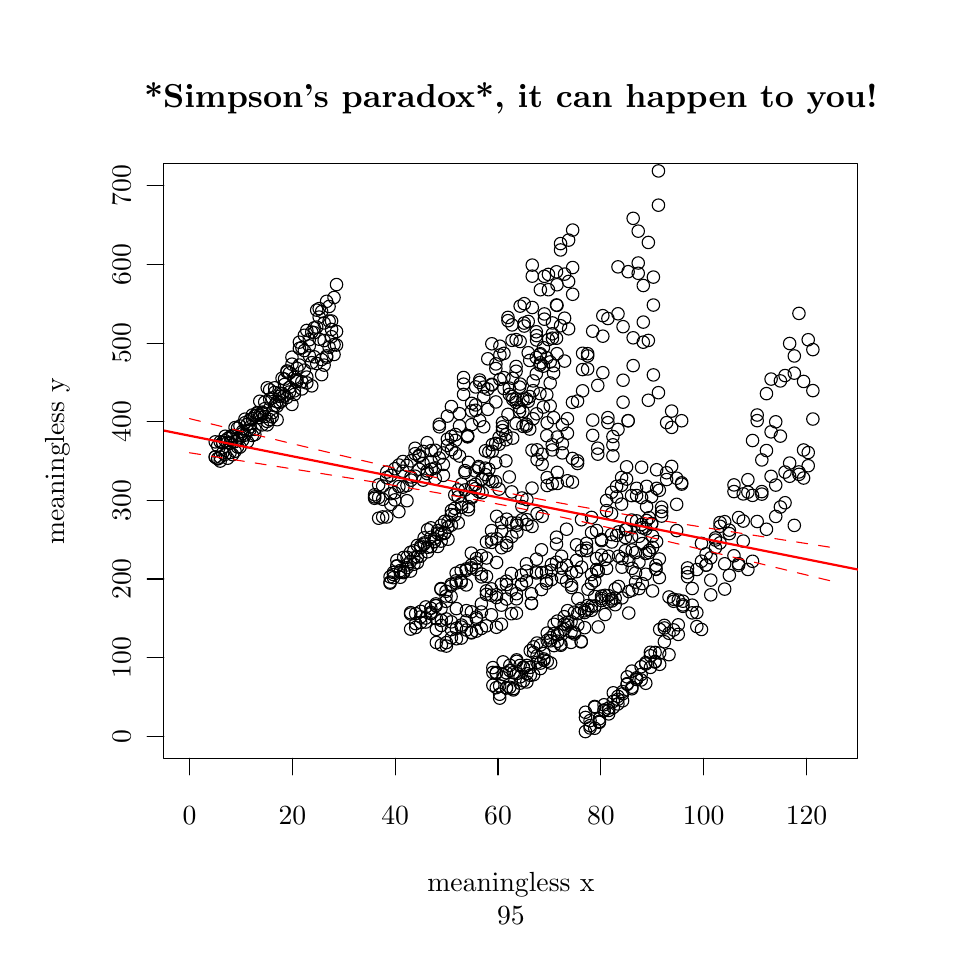
\begin{tikzpicture}[x=1pt,y=1pt]
\definecolor[named]{drawColor}{rgb}{0.00,0.00,0.00}
\definecolor[named]{fillColor}{rgb}{1.00,1.00,1.00}
\fill[color=fillColor,] (0,0) rectangle (325.21,325.21);
\begin{scope}
\path[clip] ( 49.20, 61.20) rectangle (300.01,276.01);
\definecolor[named]{drawColor}{rgb}{0.18,0.00,0.33}
\definecolor[named]{drawColor}{rgb}{0.00,0.00,0.00}

\draw[color=drawColor,line cap=round,line join=round,fill opacity=0.00,] ( 67.78,170.07) circle (  2.25);

\draw[color=drawColor,line cap=round,line join=round,fill opacity=0.00,] ( 68.67,169.52) circle (  2.25);

\draw[color=drawColor,line cap=round,line join=round,fill opacity=0.00,] ( 69.57,170.04) circle (  2.25);

\draw[color=drawColor,line cap=round,line join=round,fill opacity=0.00,] ( 70.46,171.54) circle (  2.25);

\draw[color=drawColor,line cap=round,line join=round,fill opacity=0.00,] ( 71.36,175.95) circle (  2.25);

\draw[color=drawColor,line cap=round,line join=round,fill opacity=0.00,] ( 72.25,176.72) circle (  2.25);

\draw[color=drawColor,line cap=round,line join=round,fill opacity=0.00,] ( 73.14,171.70) circle (  2.25);

\draw[color=drawColor,line cap=round,line join=round,fill opacity=0.00,] ( 74.04,177.81) circle (  2.25);

\draw[color=drawColor,line cap=round,line join=round,fill opacity=0.00,] ( 74.93,180.69) circle (  2.25);

\draw[color=drawColor,line cap=round,line join=round,fill opacity=0.00,] ( 75.83,176.29) circle (  2.25);

\draw[color=drawColor,line cap=round,line join=round,fill opacity=0.00,] ( 76.72,181.26) circle (  2.25);

\draw[color=drawColor,line cap=round,line join=round,fill opacity=0.00,] ( 77.62,178.55) circle (  2.25);

\draw[color=drawColor,line cap=round,line join=round,fill opacity=0.00,] ( 78.51,182.45) circle (  2.25);

\draw[color=drawColor,line cap=round,line join=round,fill opacity=0.00,] ( 79.40,181.91) circle (  2.25);

\draw[color=drawColor,line cap=round,line join=round,fill opacity=0.00,] ( 80.30,179.85) circle (  2.25);

\draw[color=drawColor,line cap=round,line join=round,fill opacity=0.00,] ( 81.19,185.24) circle (  2.25);

\draw[color=drawColor,line cap=round,line join=round,fill opacity=0.00,] ( 82.09,184.92) circle (  2.25);

\draw[color=drawColor,line cap=round,line join=round,fill opacity=0.00,] ( 82.98,185.23) circle (  2.25);

\draw[color=drawColor,line cap=round,line join=round,fill opacity=0.00,] ( 83.87,185.23) circle (  2.25);

\draw[color=drawColor,line cap=round,line join=round,fill opacity=0.00,] ( 84.77,186.27) circle (  2.25);

\draw[color=drawColor,line cap=round,line join=round,fill opacity=0.00,] ( 85.66,189.92) circle (  2.25);

\draw[color=drawColor,line cap=round,line join=round,fill opacity=0.00,] ( 86.56,195.08) circle (  2.25);

\draw[color=drawColor,line cap=round,line join=round,fill opacity=0.00,] ( 87.45,183.59) circle (  2.25);

\draw[color=drawColor,line cap=round,line join=round,fill opacity=0.00,] ( 88.35,191.36) circle (  2.25);

\draw[color=drawColor,line cap=round,line join=round,fill opacity=0.00,] ( 89.24,195.07) circle (  2.25);

\draw[color=drawColor,line cap=round,line join=round,fill opacity=0.00,] ( 90.13,188.45) circle (  2.25);

\draw[color=drawColor,line cap=round,line join=round,fill opacity=0.00,] ( 91.03,193.10) circle (  2.25);

\draw[color=drawColor,line cap=round,line join=round,fill opacity=0.00,] ( 91.92,198.51) circle (  2.25);

\draw[color=drawColor,line cap=round,line join=round,fill opacity=0.00,] ( 92.82,196.27) circle (  2.25);

\draw[color=drawColor,line cap=round,line join=round,fill opacity=0.00,] ( 93.71,191.59) circle (  2.25);

\draw[color=drawColor,line cap=round,line join=round,fill opacity=0.00,] ( 94.61,193.56) circle (  2.25);

\draw[color=drawColor,line cap=round,line join=round,fill opacity=0.00,] ( 95.50,206.14) circle (  2.25);

\draw[color=drawColor,line cap=round,line join=round,fill opacity=0.00,] ( 96.39,192.68) circle (  2.25);

\draw[color=drawColor,line cap=round,line join=round,fill opacity=0.00,] ( 97.29,197.94) circle (  2.25);

\draw[color=drawColor,line cap=round,line join=round,fill opacity=0.00,] ( 98.18,209.29) circle (  2.25);

\draw[color=drawColor,line cap=round,line join=round,fill opacity=0.00,] ( 99.08,194.66) circle (  2.25);

\draw[color=drawColor,line cap=round,line join=round,fill opacity=0.00,] ( 99.97,208.52) circle (  2.25);

\draw[color=drawColor,line cap=round,line join=round,fill opacity=0.00,] (100.86,198.95) circle (  2.25);

\draw[color=drawColor,line cap=round,line join=round,fill opacity=0.00,] (101.76,206.67) circle (  2.25);

\draw[color=drawColor,line cap=round,line join=round,fill opacity=0.00,] (102.65,195.77) circle (  2.25);

\draw[color=drawColor,line cap=round,line join=round,fill opacity=0.00,] (103.55,216.74) circle (  2.25);

\draw[color=drawColor,line cap=round,line join=round,fill opacity=0.00,] (104.44,223.15) circle (  2.25);

\draw[color=drawColor,line cap=round,line join=round,fill opacity=0.00,] (105.34,220.64) circle (  2.25);

\draw[color=drawColor,line cap=round,line join=round,fill opacity=0.00,] (106.23,205.27) circle (  2.25);

\draw[color=drawColor,line cap=round,line join=round,fill opacity=0.00,] (107.12,218.51) circle (  2.25);

\draw[color=drawColor,line cap=round,line join=round,fill opacity=0.00,] (108.02,206.09) circle (  2.25);

\draw[color=drawColor,line cap=round,line join=round,fill opacity=0.00,] (108.91,219.19) circle (  2.25);

\draw[color=drawColor,line cap=round,line join=round,fill opacity=0.00,] (109.81,213.53) circle (  2.25);

\draw[color=drawColor,line cap=round,line join=round,fill opacity=0.00,] (110.70,207.11) circle (  2.25);

\draw[color=drawColor,line cap=round,line join=round,fill opacity=0.00,] (111.60,210.53) circle (  2.25);

\draw[color=drawColor,line cap=round,line join=round,fill opacity=0.00,] ( 67.78,175.54) circle (  2.25);

\draw[color=drawColor,line cap=round,line join=round,fill opacity=0.00,] ( 68.67,174.10) circle (  2.25);

\draw[color=drawColor,line cap=round,line join=round,fill opacity=0.00,] ( 69.57,168.60) circle (  2.25);

\draw[color=drawColor,line cap=round,line join=round,fill opacity=0.00,] ( 70.46,175.23) circle (  2.25);

\draw[color=drawColor,line cap=round,line join=round,fill opacity=0.00,] ( 71.36,177.57) circle (  2.25);

\draw[color=drawColor,line cap=round,line join=round,fill opacity=0.00,] ( 72.25,175.36) circle (  2.25);

\draw[color=drawColor,line cap=round,line join=round,fill opacity=0.00,] ( 73.14,175.00) circle (  2.25);

\draw[color=drawColor,line cap=round,line join=round,fill opacity=0.00,] ( 74.04,177.58) circle (  2.25);

\draw[color=drawColor,line cap=round,line join=round,fill opacity=0.00,] ( 74.93,172.14) circle (  2.25);

\draw[color=drawColor,line cap=round,line join=round,fill opacity=0.00,] ( 75.83,173.71) circle (  2.25);

\draw[color=drawColor,line cap=round,line join=round,fill opacity=0.00,] ( 76.72,173.63) circle (  2.25);

\draw[color=drawColor,line cap=round,line join=round,fill opacity=0.00,] ( 77.62,179.32) circle (  2.25);

\draw[color=drawColor,line cap=round,line join=round,fill opacity=0.00,] ( 78.51,177.97) circle (  2.25);

\draw[color=drawColor,line cap=round,line join=round,fill opacity=0.00,] ( 79.40,175.60) circle (  2.25);

\draw[color=drawColor,line cap=round,line join=round,fill opacity=0.00,] ( 80.30,183.55) circle (  2.25);

\draw[color=drawColor,line cap=round,line join=round,fill opacity=0.00,] ( 81.19,177.85) circle (  2.25);

\draw[color=drawColor,line cap=round,line join=round,fill opacity=0.00,] ( 82.09,180.07) circle (  2.25);

\draw[color=drawColor,line cap=round,line join=round,fill opacity=0.00,] ( 82.98,186.14) circle (  2.25);

\draw[color=drawColor,line cap=round,line join=round,fill opacity=0.00,] ( 83.87,190.21) circle (  2.25);

\draw[color=drawColor,line cap=round,line join=round,fill opacity=0.00,] ( 84.77,185.80) circle (  2.25);

\draw[color=drawColor,line cap=round,line join=round,fill opacity=0.00,] ( 85.66,184.69) circle (  2.25);

\draw[color=drawColor,line cap=round,line join=round,fill opacity=0.00,] ( 86.56,181.69) circle (  2.25);

\draw[color=drawColor,line cap=round,line join=round,fill opacity=0.00,] ( 87.45,194.35) circle (  2.25);

\draw[color=drawColor,line cap=round,line join=round,fill opacity=0.00,] ( 88.35,184.59) circle (  2.25);

\draw[color=drawColor,line cap=round,line join=round,fill opacity=0.00,] ( 89.24,188.65) circle (  2.25);

\draw[color=drawColor,line cap=round,line join=round,fill opacity=0.00,] ( 90.13,183.54) circle (  2.25);

\draw[color=drawColor,line cap=round,line join=round,fill opacity=0.00,] ( 91.03,189.81) circle (  2.25);

\draw[color=drawColor,line cap=round,line join=round,fill opacity=0.00,] ( 91.92,193.02) circle (  2.25);

\draw[color=drawColor,line cap=round,line join=round,fill opacity=0.00,] ( 92.82,198.23) circle (  2.25);

\draw[color=drawColor,line cap=round,line join=round,fill opacity=0.00,] ( 93.71,201.16) circle (  2.25);

\draw[color=drawColor,line cap=round,line join=round,fill opacity=0.00,] ( 94.61,200.42) circle (  2.25);

\draw[color=drawColor,line cap=round,line join=round,fill opacity=0.00,] ( 95.50,189.06) circle (  2.25);

\draw[color=drawColor,line cap=round,line join=round,fill opacity=0.00,] ( 96.39,193.97) circle (  2.25);

\draw[color=drawColor,line cap=round,line join=round,fill opacity=0.00,] ( 97.29,197.34) circle (  2.25);

\draw[color=drawColor,line cap=round,line join=round,fill opacity=0.00,] ( 98.18,211.56) circle (  2.25);

\draw[color=drawColor,line cap=round,line join=round,fill opacity=0.00,] ( 99.08,197.24) circle (  2.25);

\draw[color=drawColor,line cap=round,line join=round,fill opacity=0.00,] ( 99.97,214.05) circle (  2.25);

\draw[color=drawColor,line cap=round,line join=round,fill opacity=0.00,] (100.86,215.81) circle (  2.25);

\draw[color=drawColor,line cap=round,line join=round,fill opacity=0.00,] (101.76,212.45) circle (  2.25);

\draw[color=drawColor,line cap=round,line join=round,fill opacity=0.00,] (102.65,215.21) circle (  2.25);

\draw[color=drawColor,line cap=round,line join=round,fill opacity=0.00,] (103.55,206.27) circle (  2.25);

\draw[color=drawColor,line cap=round,line join=round,fill opacity=0.00,] (104.44,203.85) circle (  2.25);

\draw[color=drawColor,line cap=round,line join=round,fill opacity=0.00,] (105.34,212.64) circle (  2.25);

\draw[color=drawColor,line cap=round,line join=round,fill opacity=0.00,] (106.23,199.82) circle (  2.25);

\draw[color=drawColor,line cap=round,line join=round,fill opacity=0.00,] (107.12,212.15) circle (  2.25);

\draw[color=drawColor,line cap=round,line join=round,fill opacity=0.00,] (108.02,226.32) circle (  2.25);

\draw[color=drawColor,line cap=round,line join=round,fill opacity=0.00,] (108.91,224.45) circle (  2.25);

\draw[color=drawColor,line cap=round,line join=round,fill opacity=0.00,] (109.81,216.16) circle (  2.25);

\draw[color=drawColor,line cap=round,line join=round,fill opacity=0.00,] (110.70,227.70) circle (  2.25);

\draw[color=drawColor,line cap=round,line join=round,fill opacity=0.00,] (111.60,215.41) circle (  2.25);

\draw[color=drawColor,line cap=round,line join=round,fill opacity=0.00,] ( 67.78,170.07) circle (  2.25);

\draw[color=drawColor,line cap=round,line join=round,fill opacity=0.00,] ( 68.67,169.40) circle (  2.25);

\draw[color=drawColor,line cap=round,line join=round,fill opacity=0.00,] ( 69.57,175.55) circle (  2.25);

\draw[color=drawColor,line cap=round,line join=round,fill opacity=0.00,] ( 70.46,175.35) circle (  2.25);

\draw[color=drawColor,line cap=round,line join=round,fill opacity=0.00,] ( 71.36,171.02) circle (  2.25);

\draw[color=drawColor,line cap=round,line join=round,fill opacity=0.00,] ( 72.25,169.64) circle (  2.25);

\draw[color=drawColor,line cap=round,line join=round,fill opacity=0.00,] ( 73.14,177.35) circle (  2.25);

\draw[color=drawColor,line cap=round,line join=round,fill opacity=0.00,] ( 74.04,170.91) circle (  2.25);

\draw[color=drawColor,line cap=round,line join=round,fill opacity=0.00,] ( 74.93,175.63) circle (  2.25);

\draw[color=drawColor,line cap=round,line join=round,fill opacity=0.00,] ( 75.83,180.48) circle (  2.25);

\draw[color=drawColor,line cap=round,line join=round,fill opacity=0.00,] ( 76.72,177.29) circle (  2.25);

\draw[color=drawColor,line cap=round,line join=round,fill opacity=0.00,] ( 77.62,176.08) circle (  2.25);

\draw[color=drawColor,line cap=round,line join=round,fill opacity=0.00,] ( 78.51,183.73) circle (  2.25);

\draw[color=drawColor,line cap=round,line join=round,fill opacity=0.00,] ( 79.40,179.65) circle (  2.25);

\draw[color=drawColor,line cap=round,line join=round,fill opacity=0.00,] ( 80.30,180.93) circle (  2.25);

\draw[color=drawColor,line cap=round,line join=round,fill opacity=0.00,] ( 81.19,183.94) circle (  2.25);

\draw[color=drawColor,line cap=round,line join=round,fill opacity=0.00,] ( 82.09,178.21) circle (  2.25);

\draw[color=drawColor,line cap=round,line join=round,fill opacity=0.00,] ( 82.98,185.91) circle (  2.25);

\draw[color=drawColor,line cap=round,line join=round,fill opacity=0.00,] ( 83.87,184.35) circle (  2.25);

\draw[color=drawColor,line cap=round,line join=round,fill opacity=0.00,] ( 84.77,181.69) circle (  2.25);

\draw[color=drawColor,line cap=round,line join=round,fill opacity=0.00,] ( 85.66,187.52) circle (  2.25);

\draw[color=drawColor,line cap=round,line join=round,fill opacity=0.00,] ( 86.56,182.93) circle (  2.25);

\draw[color=drawColor,line cap=round,line join=round,fill opacity=0.00,] ( 87.45,190.97) circle (  2.25);

\draw[color=drawColor,line cap=round,line join=round,fill opacity=0.00,] ( 88.35,186.04) circle (  2.25);

\draw[color=drawColor,line cap=round,line join=round,fill opacity=0.00,] ( 89.24,193.40) circle (  2.25);

\draw[color=drawColor,line cap=round,line join=round,fill opacity=0.00,] ( 90.13,190.07) circle (  2.25);

\draw[color=drawColor,line cap=round,line join=round,fill opacity=0.00,] ( 91.03,192.01) circle (  2.25);

\draw[color=drawColor,line cap=round,line join=round,fill opacity=0.00,] ( 91.92,190.34) circle (  2.25);

\draw[color=drawColor,line cap=round,line join=round,fill opacity=0.00,] ( 92.82,192.18) circle (  2.25);

\draw[color=drawColor,line cap=round,line join=round,fill opacity=0.00,] ( 93.71,200.78) circle (  2.25);

\draw[color=drawColor,line cap=round,line join=round,fill opacity=0.00,] ( 94.61,195.23) circle (  2.25);

\draw[color=drawColor,line cap=round,line join=round,fill opacity=0.00,] ( 95.50,203.62) circle (  2.25);

\draw[color=drawColor,line cap=round,line join=round,fill opacity=0.00,] ( 96.39,198.81) circle (  2.25);

\draw[color=drawColor,line cap=round,line join=round,fill opacity=0.00,] ( 97.29,202.13) circle (  2.25);

\draw[color=drawColor,line cap=round,line join=round,fill opacity=0.00,] ( 98.18,203.30) circle (  2.25);

\draw[color=drawColor,line cap=round,line join=round,fill opacity=0.00,] ( 99.08,209.61) circle (  2.25);

\draw[color=drawColor,line cap=round,line join=round,fill opacity=0.00,] ( 99.97,201.46) circle (  2.25);

\draw[color=drawColor,line cap=round,line join=round,fill opacity=0.00,] (100.86,196.83) circle (  2.25);

\draw[color=drawColor,line cap=round,line join=round,fill opacity=0.00,] (101.76,210.24) circle (  2.25);

\draw[color=drawColor,line cap=round,line join=round,fill opacity=0.00,] (102.65,204.15) circle (  2.25);

\draw[color=drawColor,line cap=round,line join=round,fill opacity=0.00,] (103.55,215.00) circle (  2.25);

\draw[color=drawColor,line cap=round,line join=round,fill opacity=0.00,] (104.44,217.01) circle (  2.25);

\draw[color=drawColor,line cap=round,line join=round,fill opacity=0.00,] (105.34,223.69) circle (  2.25);

\draw[color=drawColor,line cap=round,line join=round,fill opacity=0.00,] (106.23,222.64) circle (  2.25);

\draw[color=drawColor,line cap=round,line join=round,fill opacity=0.00,] (107.12,203.27) circle (  2.25);

\draw[color=drawColor,line cap=round,line join=round,fill opacity=0.00,] (108.02,206.61) circle (  2.25);

\draw[color=drawColor,line cap=round,line join=round,fill opacity=0.00,] (108.91,209.73) circle (  2.25);

\draw[color=drawColor,line cap=round,line join=round,fill opacity=0.00,] (109.81,219.21) circle (  2.25);

\draw[color=drawColor,line cap=round,line join=round,fill opacity=0.00,] (110.70,210.70) circle (  2.25);

\draw[color=drawColor,line cap=round,line join=round,fill opacity=0.00,] (111.60,232.38) circle (  2.25);

\draw[color=drawColor,line cap=round,line join=round,fill opacity=0.00,] (125.37,155.16) circle (  2.25);

\draw[color=drawColor,line cap=round,line join=round,fill opacity=0.00,] (126.83,159.99) circle (  2.25);

\draw[color=drawColor,line cap=round,line join=round,fill opacity=0.00,] (128.29,159.59) circle (  2.25);

\draw[color=drawColor,line cap=round,line join=round,fill opacity=0.00,] (129.75,148.39) circle (  2.25);

\draw[color=drawColor,line cap=round,line join=round,fill opacity=0.00,] (131.21,163.44) circle (  2.25);

\draw[color=drawColor,line cap=round,line join=round,fill opacity=0.00,] (132.68,154.58) circle (  2.25);

\draw[color=drawColor,line cap=round,line join=round,fill opacity=0.00,] (134.14,150.31) circle (  2.25);

\draw[color=drawColor,line cap=round,line join=round,fill opacity=0.00,] (135.60,164.93) circle (  2.25);

\draw[color=drawColor,line cap=round,line join=round,fill opacity=0.00,] (137.06,154.27) circle (  2.25);

\draw[color=drawColor,line cap=round,line join=round,fill opacity=0.00,] (138.52,162.86) circle (  2.25);

\draw[color=drawColor,line cap=round,line join=round,fill opacity=0.00,] (139.98,171.25) circle (  2.25);

\draw[color=drawColor,line cap=round,line join=round,fill opacity=0.00,] (141.44,170.30) circle (  2.25);

\draw[color=drawColor,line cap=round,line join=round,fill opacity=0.00,] (142.90,167.74) circle (  2.25);

\draw[color=drawColor,line cap=round,line join=round,fill opacity=0.00,] (144.36,175.26) circle (  2.25);

\draw[color=drawColor,line cap=round,line join=round,fill opacity=0.00,] (145.82,165.65) circle (  2.25);

\draw[color=drawColor,line cap=round,line join=round,fill opacity=0.00,] (147.28,162.24) circle (  2.25);

\draw[color=drawColor,line cap=round,line join=round,fill opacity=0.00,] (148.74,180.98) circle (  2.25);

\draw[color=drawColor,line cap=round,line join=round,fill opacity=0.00,] (150.20,163.42) circle (  2.25);

\draw[color=drawColor,line cap=round,line join=round,fill opacity=0.00,] (151.66,176.50) circle (  2.25);

\draw[color=drawColor,line cap=round,line join=round,fill opacity=0.00,] (153.12,177.49) circle (  2.25);

\draw[color=drawColor,line cap=round,line join=round,fill opacity=0.00,] (154.58,176.08) circle (  2.25);

\draw[color=drawColor,line cap=round,line join=round,fill opacity=0.00,] (156.04,185.71) circle (  2.25);

\draw[color=drawColor,line cap=round,line join=round,fill opacity=0.00,] (157.50,196.39) circle (  2.25);

\draw[color=drawColor,line cap=round,line join=round,fill opacity=0.00,] (158.96,177.37) circle (  2.25);

\draw[color=drawColor,line cap=round,line join=round,fill opacity=0.00,] (160.42,181.74) circle (  2.25);

\draw[color=drawColor,line cap=round,line join=round,fill opacity=0.00,] (161.88,186.95) circle (  2.25);

\draw[color=drawColor,line cap=round,line join=round,fill opacity=0.00,] (163.34,183.23) circle (  2.25);

\draw[color=drawColor,line cap=round,line join=round,fill opacity=0.00,] (164.80,195.31) circle (  2.25);

\draw[color=drawColor,line cap=round,line join=round,fill opacity=0.00,] (166.26,187.28) circle (  2.25);

\draw[color=drawColor,line cap=round,line join=round,fill opacity=0.00,] (167.72,210.98) circle (  2.25);

\draw[color=drawColor,line cap=round,line join=round,fill opacity=0.00,] (169.18,189.96) circle (  2.25);

\draw[color=drawColor,line cap=round,line join=round,fill opacity=0.00,] (170.64,206.93) circle (  2.25);

\draw[color=drawColor,line cap=round,line join=round,fill opacity=0.00,] (172.10,207.52) circle (  2.25);

\draw[color=drawColor,line cap=round,line join=round,fill opacity=0.00,] (173.56,220.51) circle (  2.25);

\draw[color=drawColor,line cap=round,line join=round,fill opacity=0.00,] (175.02,191.97) circle (  2.25);

\draw[color=drawColor,line cap=round,line join=round,fill opacity=0.00,] (176.49,202.78) circle (  2.25);

\draw[color=drawColor,line cap=round,line join=round,fill opacity=0.00,] (177.95,211.80) circle (  2.25);

\draw[color=drawColor,line cap=round,line join=round,fill opacity=0.00,] (179.41,225.48) circle (  2.25);

\draw[color=drawColor,line cap=round,line join=round,fill opacity=0.00,] (180.87,207.75) circle (  2.25);

\draw[color=drawColor,line cap=round,line join=round,fill opacity=0.00,] (182.33,235.42) circle (  2.25);

\draw[color=drawColor,line cap=round,line join=round,fill opacity=0.00,] (183.79,206.00) circle (  2.25);

\draw[color=drawColor,line cap=round,line join=round,fill opacity=0.00,] (185.25,207.39) circle (  2.25);

\draw[color=drawColor,line cap=round,line join=round,fill opacity=0.00,] (186.71,219.88) circle (  2.25);

\draw[color=drawColor,line cap=round,line join=round,fill opacity=0.00,] (188.17,212.49) circle (  2.25);

\draw[color=drawColor,line cap=round,line join=round,fill opacity=0.00,] (189.63,213.00) circle (  2.25);

\draw[color=drawColor,line cap=round,line join=round,fill opacity=0.00,] (191.09,225.01) circle (  2.25);

\draw[color=drawColor,line cap=round,line join=round,fill opacity=0.00,] (192.55,244.88) circle (  2.25);

\draw[color=drawColor,line cap=round,line join=round,fill opacity=0.00,] (194.01,220.23) circle (  2.25);

\draw[color=drawColor,line cap=round,line join=round,fill opacity=0.00,] (195.47,248.45) circle (  2.25);

\draw[color=drawColor,line cap=round,line join=round,fill opacity=0.00,] (196.93,228.87) circle (  2.25);

\draw[color=drawColor,line cap=round,line join=round,fill opacity=0.00,] (125.37,156.42) circle (  2.25);

\draw[color=drawColor,line cap=round,line join=round,fill opacity=0.00,] (126.83,147.95) circle (  2.25);

\draw[color=drawColor,line cap=round,line join=round,fill opacity=0.00,] (128.29,154.79) circle (  2.25);

\draw[color=drawColor,line cap=round,line join=round,fill opacity=0.00,] (129.75,162.62) circle (  2.25);

\draw[color=drawColor,line cap=round,line join=round,fill opacity=0.00,] (131.21,152.97) circle (  2.25);

\draw[color=drawColor,line cap=round,line join=round,fill opacity=0.00,] (132.68,165.83) circle (  2.25);

\draw[color=drawColor,line cap=round,line join=round,fill opacity=0.00,] (134.14,159.38) circle (  2.25);

\draw[color=drawColor,line cap=round,line join=round,fill opacity=0.00,] (135.60,168.44) circle (  2.25);

\draw[color=drawColor,line cap=round,line join=round,fill opacity=0.00,] (137.06,159.79) circle (  2.25);

\draw[color=drawColor,line cap=round,line join=round,fill opacity=0.00,] (138.52,168.67) circle (  2.25);

\draw[color=drawColor,line cap=round,line join=round,fill opacity=0.00,] (139.98,163.14) circle (  2.25);

\draw[color=drawColor,line cap=round,line join=round,fill opacity=0.00,] (141.44,170.67) circle (  2.25);

\draw[color=drawColor,line cap=round,line join=round,fill opacity=0.00,] (142.90,172.07) circle (  2.25);

\draw[color=drawColor,line cap=round,line join=round,fill opacity=0.00,] (144.36,164.09) circle (  2.25);

\draw[color=drawColor,line cap=round,line join=round,fill opacity=0.00,] (145.82,172.40) circle (  2.25);

\draw[color=drawColor,line cap=round,line join=round,fill opacity=0.00,] (147.28,166.10) circle (  2.25);

\draw[color=drawColor,line cap=round,line join=round,fill opacity=0.00,] (148.74,181.90) circle (  2.25);

\draw[color=drawColor,line cap=round,line join=round,fill opacity=0.00,] (150.20,167.38) circle (  2.25);

\draw[color=drawColor,line cap=round,line join=round,fill opacity=0.00,] (151.66,174.23) circle (  2.25);

\draw[color=drawColor,line cap=round,line join=round,fill opacity=0.00,] (153.12,188.30) circle (  2.25);

\draw[color=drawColor,line cap=round,line join=round,fill opacity=0.00,] (154.58,178.19) circle (  2.25);

\draw[color=drawColor,line cap=round,line join=round,fill opacity=0.00,] (156.04,181.30) circle (  2.25);

\draw[color=drawColor,line cap=round,line join=round,fill opacity=0.00,] (157.50,192.69) circle (  2.25);

\draw[color=drawColor,line cap=round,line join=round,fill opacity=0.00,] (158.96,177.85) circle (  2.25);

\draw[color=drawColor,line cap=round,line join=round,fill opacity=0.00,] (160.42,189.46) circle (  2.25);

\draw[color=drawColor,line cap=round,line join=round,fill opacity=0.00,] (161.88,188.89) circle (  2.25);

\draw[color=drawColor,line cap=round,line join=round,fill opacity=0.00,] (163.34,197.02) circle (  2.25);

\draw[color=drawColor,line cap=round,line join=round,fill opacity=0.00,] (164.80,180.98) circle (  2.25);

\draw[color=drawColor,line cap=round,line join=round,fill opacity=0.00,] (166.26,205.56) circle (  2.25);

\draw[color=drawColor,line cap=round,line join=round,fill opacity=0.00,] (167.72,196.10) circle (  2.25);

\draw[color=drawColor,line cap=round,line join=round,fill opacity=0.00,] (169.18,203.69) circle (  2.25);

\draw[color=drawColor,line cap=round,line join=round,fill opacity=0.00,] (170.64,210.10) circle (  2.25);

\draw[color=drawColor,line cap=round,line join=round,fill opacity=0.00,] (172.10,194.83) circle (  2.25);

\draw[color=drawColor,line cap=round,line join=round,fill opacity=0.00,] (173.56,219.33) circle (  2.25);

\draw[color=drawColor,line cap=round,line join=round,fill opacity=0.00,] (175.02,217.80) circle (  2.25);

\draw[color=drawColor,line cap=round,line join=round,fill opacity=0.00,] (176.49,212.48) circle (  2.25);

\draw[color=drawColor,line cap=round,line join=round,fill opacity=0.00,] (177.95,196.42) circle (  2.25);

\draw[color=drawColor,line cap=round,line join=round,fill opacity=0.00,] (179.41,218.47) circle (  2.25);

\draw[color=drawColor,line cap=round,line join=round,fill opacity=0.00,] (180.87,219.04) circle (  2.25);

\draw[color=drawColor,line cap=round,line join=round,fill opacity=0.00,] (182.33,239.41) circle (  2.25);

\draw[color=drawColor,line cap=round,line join=round,fill opacity=0.00,] (183.79,200.13) circle (  2.25);

\draw[color=drawColor,line cap=round,line join=round,fill opacity=0.00,] (185.25,230.51) circle (  2.25);

\draw[color=drawColor,line cap=round,line join=round,fill opacity=0.00,] (186.71,235.36) circle (  2.25);

\draw[color=drawColor,line cap=round,line join=round,fill opacity=0.00,] (188.17,230.52) circle (  2.25);

\draw[color=drawColor,line cap=round,line join=round,fill opacity=0.00,] (189.63,218.51) circle (  2.25);

\draw[color=drawColor,line cap=round,line join=round,fill opacity=0.00,] (191.09,236.99) circle (  2.25);

\draw[color=drawColor,line cap=round,line join=round,fill opacity=0.00,] (192.55,247.18) circle (  2.25);

\draw[color=drawColor,line cap=round,line join=round,fill opacity=0.00,] (194.01,236.16) circle (  2.25);

\draw[color=drawColor,line cap=round,line join=round,fill opacity=0.00,] (195.47,216.39) circle (  2.25);

\draw[color=drawColor,line cap=round,line join=round,fill opacity=0.00,] (196.93,238.53) circle (  2.25);

\draw[color=drawColor,line cap=round,line join=round,fill opacity=0.00,] (125.37,155.66) circle (  2.25);

\draw[color=drawColor,line cap=round,line join=round,fill opacity=0.00,] (126.83,155.45) circle (  2.25);

\draw[color=drawColor,line cap=round,line join=round,fill opacity=0.00,] (128.29,148.41) circle (  2.25);

\draw[color=drawColor,line cap=round,line join=round,fill opacity=0.00,] (129.75,164.62) circle (  2.25);

\draw[color=drawColor,line cap=round,line join=round,fill opacity=0.00,] (131.21,156.82) circle (  2.25);

\draw[color=drawColor,line cap=round,line join=round,fill opacity=0.00,] (132.68,157.14) circle (  2.25);

\draw[color=drawColor,line cap=round,line join=round,fill opacity=0.00,] (134.14,167.17) circle (  2.25);

\draw[color=drawColor,line cap=round,line join=round,fill opacity=0.00,] (135.60,159.18) circle (  2.25);

\draw[color=drawColor,line cap=round,line join=round,fill opacity=0.00,] (137.06,167.04) circle (  2.25);

\draw[color=drawColor,line cap=round,line join=round,fill opacity=0.00,] (138.52,161.72) circle (  2.25);

\draw[color=drawColor,line cap=round,line join=round,fill opacity=0.00,] (139.98,173.23) circle (  2.25);

\draw[color=drawColor,line cap=round,line join=round,fill opacity=0.00,] (141.44,165.64) circle (  2.25);

\draw[color=drawColor,line cap=round,line join=round,fill opacity=0.00,] (142.90,161.71) circle (  2.25);

\draw[color=drawColor,line cap=round,line join=round,fill opacity=0.00,] (144.36,165.06) circle (  2.25);

\draw[color=drawColor,line cap=round,line join=round,fill opacity=0.00,] (145.82,168.31) circle (  2.25);

\draw[color=drawColor,line cap=round,line join=round,fill opacity=0.00,] (147.28,172.50) circle (  2.25);

\draw[color=drawColor,line cap=round,line join=round,fill opacity=0.00,] (148.74,169.68) circle (  2.25);

\draw[color=drawColor,line cap=round,line join=round,fill opacity=0.00,] (150.20,171.52) circle (  2.25);

\draw[color=drawColor,line cap=round,line join=round,fill opacity=0.00,] (151.66,184.84) circle (  2.25);

\draw[color=drawColor,line cap=round,line join=round,fill opacity=0.00,] (153.12,172.76) circle (  2.25);

\draw[color=drawColor,line cap=round,line join=round,fill opacity=0.00,] (154.58,171.46) circle (  2.25);

\draw[color=drawColor,line cap=round,line join=round,fill opacity=0.00,] (156.04,170.41) circle (  2.25);

\draw[color=drawColor,line cap=round,line join=round,fill opacity=0.00,] (157.50,198.79) circle (  2.25);

\draw[color=drawColor,line cap=round,line join=round,fill opacity=0.00,] (158.96,177.45) circle (  2.25);

\draw[color=drawColor,line cap=round,line join=round,fill opacity=0.00,] (160.42,186.70) circle (  2.25);

\draw[color=drawColor,line cap=round,line join=round,fill opacity=0.00,] (161.88,195.38) circle (  2.25);

\draw[color=drawColor,line cap=round,line join=round,fill opacity=0.00,] (163.34,197.89) circle (  2.25);

\draw[color=drawColor,line cap=round,line join=round,fill opacity=0.00,] (164.80,191.93) circle (  2.25);

\draw[color=drawColor,line cap=round,line join=round,fill opacity=0.00,] (166.26,194.59) circle (  2.25);

\draw[color=drawColor,line cap=round,line join=round,fill opacity=0.00,] (167.72,196.34) circle (  2.25);

\draw[color=drawColor,line cap=round,line join=round,fill opacity=0.00,] (169.18,202.03) circle (  2.25);

\draw[color=drawColor,line cap=round,line join=round,fill opacity=0.00,] (170.64,198.15) circle (  2.25);

\draw[color=drawColor,line cap=round,line join=round,fill opacity=0.00,] (172.10,198.73) circle (  2.25);

\draw[color=drawColor,line cap=round,line join=round,fill opacity=0.00,] (173.56,185.48) circle (  2.25);

\draw[color=drawColor,line cap=round,line join=round,fill opacity=0.00,] (175.02,212.23) circle (  2.25);

\draw[color=drawColor,line cap=round,line join=round,fill opacity=0.00,] (176.49,201.05) circle (  2.25);

\draw[color=drawColor,line cap=round,line join=round,fill opacity=0.00,] (177.95,224.59) circle (  2.25);

\draw[color=drawColor,line cap=round,line join=round,fill opacity=0.00,] (179.41,217.39) circle (  2.25);

\draw[color=drawColor,line cap=round,line join=round,fill opacity=0.00,] (180.87,190.19) circle (  2.25);

\draw[color=drawColor,line cap=round,line join=round,fill opacity=0.00,] (182.33,224.09) circle (  2.25);

\draw[color=drawColor,line cap=round,line join=round,fill opacity=0.00,] (183.79,215.32) circle (  2.25);

\draw[color=drawColor,line cap=round,line join=round,fill opacity=0.00,] (185.25,204.09) circle (  2.25);

\draw[color=drawColor,line cap=round,line join=round,fill opacity=0.00,] (186.71,221.77) circle (  2.25);

\draw[color=drawColor,line cap=round,line join=round,fill opacity=0.00,] (188.17,236.06) circle (  2.25);

\draw[color=drawColor,line cap=round,line join=round,fill opacity=0.00,] (189.63,214.59) circle (  2.25);

\draw[color=drawColor,line cap=round,line join=round,fill opacity=0.00,] (191.09,212.99) circle (  2.25);

\draw[color=drawColor,line cap=round,line join=round,fill opacity=0.00,] (192.55,217.49) circle (  2.25);

\draw[color=drawColor,line cap=round,line join=round,fill opacity=0.00,] (194.01,204.73) circle (  2.25);

\draw[color=drawColor,line cap=round,line join=round,fill opacity=0.00,] (195.47,233.50) circle (  2.25);

\draw[color=drawColor,line cap=round,line join=round,fill opacity=0.00,] (196.93,252.07) circle (  2.25);

\draw[color=drawColor,line cap=round,line join=round,fill opacity=0.00,] (130.95,124.86) circle (  2.25);

\draw[color=drawColor,line cap=round,line join=round,fill opacity=0.00,] (132.18,126.47) circle (  2.25);

\draw[color=drawColor,line cap=round,line join=round,fill opacity=0.00,] (133.41,132.75) circle (  2.25);

\draw[color=drawColor,line cap=round,line join=round,fill opacity=0.00,] (134.64,128.40) circle (  2.25);

\draw[color=drawColor,line cap=round,line join=round,fill opacity=0.00,] (135.87,133.79) circle (  2.25);

\draw[color=drawColor,line cap=round,line join=round,fill opacity=0.00,] (137.10,133.82) circle (  2.25);

\draw[color=drawColor,line cap=round,line join=round,fill opacity=0.00,] (138.33,135.62) circle (  2.25);

\draw[color=drawColor,line cap=round,line join=round,fill opacity=0.00,] (139.56,133.64) circle (  2.25);

\draw[color=drawColor,line cap=round,line join=round,fill opacity=0.00,] (140.80,138.11) circle (  2.25);

\draw[color=drawColor,line cap=round,line join=round,fill opacity=0.00,] (142.03,137.92) circle (  2.25);

\draw[color=drawColor,line cap=round,line join=round,fill opacity=0.00,] (143.26,139.02) circle (  2.25);

\draw[color=drawColor,line cap=round,line join=round,fill opacity=0.00,] (144.49,135.82) circle (  2.25);

\draw[color=drawColor,line cap=round,line join=round,fill opacity=0.00,] (145.72,144.47) circle (  2.25);

\draw[color=drawColor,line cap=round,line join=round,fill opacity=0.00,] (146.95,140.53) circle (  2.25);

\draw[color=drawColor,line cap=round,line join=round,fill opacity=0.00,] (148.18,142.52) circle (  2.25);

\draw[color=drawColor,line cap=round,line join=round,fill opacity=0.00,] (149.41,145.40) circle (  2.25);

\draw[color=drawColor,line cap=round,line join=round,fill opacity=0.00,] (150.64,142.45) circle (  2.25);

\draw[color=drawColor,line cap=round,line join=round,fill opacity=0.00,] (151.88,146.66) circle (  2.25);

\draw[color=drawColor,line cap=round,line join=round,fill opacity=0.00,] (153.11,149.26) circle (  2.25);

\draw[color=drawColor,line cap=round,line join=round,fill opacity=0.00,] (154.34,151.50) circle (  2.25);

\draw[color=drawColor,line cap=round,line join=round,fill opacity=0.00,] (155.57,158.18) circle (  2.25);

\draw[color=drawColor,line cap=round,line join=round,fill opacity=0.00,] (156.80,153.18) circle (  2.25);

\draw[color=drawColor,line cap=round,line join=round,fill opacity=0.00,] (158.03,164.44) circle (  2.25);

\draw[color=drawColor,line cap=round,line join=round,fill opacity=0.00,] (159.26,168.12) circle (  2.25);

\draw[color=drawColor,line cap=round,line join=round,fill opacity=0.00,] (160.49,159.48) circle (  2.25);

\draw[color=drawColor,line cap=round,line join=round,fill opacity=0.00,] (161.72,160.17) circle (  2.25);

\draw[color=drawColor,line cap=round,line join=round,fill opacity=0.00,] (162.96,157.59) circle (  2.25);

\draw[color=drawColor,line cap=round,line join=round,fill opacity=0.00,] (164.19,161.99) circle (  2.25);

\draw[color=drawColor,line cap=round,line join=round,fill opacity=0.00,] (165.42,172.32) circle (  2.25);

\draw[color=drawColor,line cap=round,line join=round,fill opacity=0.00,] (166.65,165.64) circle (  2.25);

\draw[color=drawColor,line cap=round,line join=round,fill opacity=0.00,] (167.88,172.13) circle (  2.25);

\draw[color=drawColor,line cap=round,line join=round,fill opacity=0.00,] (169.11,168.03) circle (  2.25);

\draw[color=drawColor,line cap=round,line join=round,fill opacity=0.00,] (170.34,177.12) circle (  2.25);

\draw[color=drawColor,line cap=round,line join=round,fill opacity=0.00,] (171.57,179.63) circle (  2.25);

\draw[color=drawColor,line cap=round,line join=round,fill opacity=0.00,] (172.80,178.16) circle (  2.25);

\draw[color=drawColor,line cap=round,line join=round,fill opacity=0.00,] (174.03,194.97) circle (  2.25);

\draw[color=drawColor,line cap=round,line join=round,fill opacity=0.00,] (175.27,198.51) circle (  2.25);

\draw[color=drawColor,line cap=round,line join=round,fill opacity=0.00,] (176.50,182.16) circle (  2.25);

\draw[color=drawColor,line cap=round,line join=round,fill opacity=0.00,] (177.73,186.50) circle (  2.25);

\draw[color=drawColor,line cap=round,line join=round,fill opacity=0.00,] (178.96,186.47) circle (  2.25);

\draw[color=drawColor,line cap=round,line join=round,fill opacity=0.00,] (180.19,181.22) circle (  2.25);

\draw[color=drawColor,line cap=round,line join=round,fill opacity=0.00,] (181.42,180.16) circle (  2.25);

\draw[color=drawColor,line cap=round,line join=round,fill opacity=0.00,] (182.65,194.02) circle (  2.25);

\draw[color=drawColor,line cap=round,line join=round,fill opacity=0.00,] (183.88,185.67) circle (  2.25);

\draw[color=drawColor,line cap=round,line join=round,fill opacity=0.00,] (185.11,192.98) circle (  2.25);

\draw[color=drawColor,line cap=round,line join=round,fill opacity=0.00,] (186.35,202.91) circle (  2.25);

\draw[color=drawColor,line cap=round,line join=round,fill opacity=0.00,] (187.58,192.58) circle (  2.25);

\draw[color=drawColor,line cap=round,line join=round,fill opacity=0.00,] (188.81,196.81) circle (  2.25);

\draw[color=drawColor,line cap=round,line join=round,fill opacity=0.00,] (190.04,184.29) circle (  2.25);

\draw[color=drawColor,line cap=round,line join=round,fill opacity=0.00,] (191.27,207.41) circle (  2.25);

\draw[color=drawColor,line cap=round,line join=round,fill opacity=0.00,] (130.95,124.52) circle (  2.25);

\draw[color=drawColor,line cap=round,line join=round,fill opacity=0.00,] (132.18,128.36) circle (  2.25);

\draw[color=drawColor,line cap=round,line join=round,fill opacity=0.00,] (133.41,130.58) circle (  2.25);

\draw[color=drawColor,line cap=round,line join=round,fill opacity=0.00,] (134.64,126.62) circle (  2.25);

\draw[color=drawColor,line cap=round,line join=round,fill opacity=0.00,] (135.87,128.68) circle (  2.25);

\draw[color=drawColor,line cap=round,line join=round,fill opacity=0.00,] (137.10,130.08) circle (  2.25);

\draw[color=drawColor,line cap=round,line join=round,fill opacity=0.00,] (138.33,132.37) circle (  2.25);

\draw[color=drawColor,line cap=round,line join=round,fill opacity=0.00,] (139.56,131.32) circle (  2.25);

\draw[color=drawColor,line cap=round,line join=round,fill opacity=0.00,] (140.80,133.97) circle (  2.25);

\draw[color=drawColor,line cap=round,line join=round,fill opacity=0.00,] (142.03,134.23) circle (  2.25);

\draw[color=drawColor,line cap=round,line join=round,fill opacity=0.00,] (143.26,138.58) circle (  2.25);

\draw[color=drawColor,line cap=round,line join=round,fill opacity=0.00,] (144.49,143.79) circle (  2.25);

\draw[color=drawColor,line cap=round,line join=round,fill opacity=0.00,] (145.72,137.68) circle (  2.25);

\draw[color=drawColor,line cap=round,line join=round,fill opacity=0.00,] (146.95,139.53) circle (  2.25);

\draw[color=drawColor,line cap=round,line join=round,fill opacity=0.00,] (148.18,137.75) circle (  2.25);

\draw[color=drawColor,line cap=round,line join=round,fill opacity=0.00,] (149.41,142.23) circle (  2.25);

\draw[color=drawColor,line cap=round,line join=round,fill opacity=0.00,] (150.64,146.79) circle (  2.25);

\draw[color=drawColor,line cap=round,line join=round,fill opacity=0.00,] (151.88,144.71) circle (  2.25);

\draw[color=drawColor,line cap=round,line join=round,fill opacity=0.00,] (153.11,145.46) circle (  2.25);

\draw[color=drawColor,line cap=round,line join=round,fill opacity=0.00,] (154.34,156.37) circle (  2.25);

\draw[color=drawColor,line cap=round,line join=round,fill opacity=0.00,] (155.57,155.65) circle (  2.25);

\draw[color=drawColor,line cap=round,line join=round,fill opacity=0.00,] (156.80,151.89) circle (  2.25);

\draw[color=drawColor,line cap=round,line join=round,fill opacity=0.00,] (158.03,165.13) circle (  2.25);

\draw[color=drawColor,line cap=round,line join=round,fill opacity=0.00,] (159.26,152.14) circle (  2.25);

\draw[color=drawColor,line cap=round,line join=round,fill opacity=0.00,] (160.49,155.34) circle (  2.25);

\draw[color=drawColor,line cap=round,line join=round,fill opacity=0.00,] (161.72,165.03) circle (  2.25);

\draw[color=drawColor,line cap=round,line join=round,fill opacity=0.00,] (162.96,166.14) circle (  2.25);

\draw[color=drawColor,line cap=round,line join=round,fill opacity=0.00,] (164.19,162.14) circle (  2.25);

\draw[color=drawColor,line cap=round,line join=round,fill opacity=0.00,] (165.42,166.03) circle (  2.25);

\draw[color=drawColor,line cap=round,line join=round,fill opacity=0.00,] (166.65,171.89) circle (  2.25);

\draw[color=drawColor,line cap=round,line join=round,fill opacity=0.00,] (167.88,161.19) circle (  2.25);

\draw[color=drawColor,line cap=round,line join=round,fill opacity=0.00,] (169.11,161.14) circle (  2.25);

\draw[color=drawColor,line cap=round,line join=round,fill opacity=0.00,] (170.34,174.69) circle (  2.25);

\draw[color=drawColor,line cap=round,line join=round,fill opacity=0.00,] (171.57,180.96) circle (  2.25);

\draw[color=drawColor,line cap=round,line join=round,fill opacity=0.00,] (172.80,176.29) circle (  2.25);

\draw[color=drawColor,line cap=round,line join=round,fill opacity=0.00,] (174.03,192.70) circle (  2.25);

\draw[color=drawColor,line cap=round,line join=round,fill opacity=0.00,] (175.27,176.90) circle (  2.25);

\draw[color=drawColor,line cap=round,line join=round,fill opacity=0.00,] (176.50,189.83) circle (  2.25);

\draw[color=drawColor,line cap=round,line join=round,fill opacity=0.00,] (177.73,195.33) circle (  2.25);

\draw[color=drawColor,line cap=round,line join=round,fill opacity=0.00,] (178.96,190.80) circle (  2.25);

\draw[color=drawColor,line cap=round,line join=round,fill opacity=0.00,] (180.19,181.90) circle (  2.25);

\draw[color=drawColor,line cap=round,line join=round,fill opacity=0.00,] (181.42,204.95) circle (  2.25);

\draw[color=drawColor,line cap=round,line join=round,fill opacity=0.00,] (182.65,183.89) circle (  2.25);

\draw[color=drawColor,line cap=round,line join=round,fill opacity=0.00,] (183.88,212.35) circle (  2.25);

\draw[color=drawColor,line cap=round,line join=round,fill opacity=0.00,] (185.11,207.01) circle (  2.25);

\draw[color=drawColor,line cap=round,line join=round,fill opacity=0.00,] (186.35,209.59) circle (  2.25);

\draw[color=drawColor,line cap=round,line join=round,fill opacity=0.00,] (187.58,177.77) circle (  2.25);

\draw[color=drawColor,line cap=round,line join=round,fill opacity=0.00,] (188.81,204.43) circle (  2.25);

\draw[color=drawColor,line cap=round,line join=round,fill opacity=0.00,] (190.04,203.06) circle (  2.25);

\draw[color=drawColor,line cap=round,line join=round,fill opacity=0.00,] (191.27,224.88) circle (  2.25);

\draw[color=drawColor,line cap=round,line join=round,fill opacity=0.00,] (130.95,126.77) circle (  2.25);

\draw[color=drawColor,line cap=round,line join=round,fill opacity=0.00,] (132.18,127.59) circle (  2.25);

\draw[color=drawColor,line cap=round,line join=round,fill opacity=0.00,] (133.41,130.75) circle (  2.25);

\draw[color=drawColor,line cap=round,line join=round,fill opacity=0.00,] (134.64,129.04) circle (  2.25);

\draw[color=drawColor,line cap=round,line join=round,fill opacity=0.00,] (135.87,128.28) circle (  2.25);

\draw[color=drawColor,line cap=round,line join=round,fill opacity=0.00,] (137.10,131.05) circle (  2.25);

\draw[color=drawColor,line cap=round,line join=round,fill opacity=0.00,] (138.33,128.84) circle (  2.25);

\draw[color=drawColor,line cap=round,line join=round,fill opacity=0.00,] (139.56,136.14) circle (  2.25);

\draw[color=drawColor,line cap=round,line join=round,fill opacity=0.00,] (140.80,131.90) circle (  2.25);

\draw[color=drawColor,line cap=round,line join=round,fill opacity=0.00,] (142.03,137.34) circle (  2.25);

\draw[color=drawColor,line cap=round,line join=round,fill opacity=0.00,] (143.26,140.85) circle (  2.25);

\draw[color=drawColor,line cap=round,line join=round,fill opacity=0.00,] (144.49,137.47) circle (  2.25);

\draw[color=drawColor,line cap=round,line join=round,fill opacity=0.00,] (145.72,141.07) circle (  2.25);

\draw[color=drawColor,line cap=round,line join=round,fill opacity=0.00,] (146.95,139.49) circle (  2.25);

\draw[color=drawColor,line cap=round,line join=round,fill opacity=0.00,] (148.18,143.48) circle (  2.25);

\draw[color=drawColor,line cap=round,line join=round,fill opacity=0.00,] (149.41,139.68) circle (  2.25);

\draw[color=drawColor,line cap=round,line join=round,fill opacity=0.00,] (150.64,142.70) circle (  2.25);

\draw[color=drawColor,line cap=round,line join=round,fill opacity=0.00,] (151.88,140.38) circle (  2.25);

\draw[color=drawColor,line cap=round,line join=round,fill opacity=0.00,] (153.11,150.72) circle (  2.25);

\draw[color=drawColor,line cap=round,line join=round,fill opacity=0.00,] (154.34,149.11) circle (  2.25);

\draw[color=drawColor,line cap=round,line join=round,fill opacity=0.00,] (155.57,146.29) circle (  2.25);

\draw[color=drawColor,line cap=round,line join=round,fill opacity=0.00,] (156.80,160.30) circle (  2.25);

\draw[color=drawColor,line cap=round,line join=round,fill opacity=0.00,] (158.03,158.16) circle (  2.25);

\draw[color=drawColor,line cap=round,line join=round,fill opacity=0.00,] (159.26,150.98) circle (  2.25);

\draw[color=drawColor,line cap=round,line join=round,fill opacity=0.00,] (160.49,155.74) circle (  2.25);

\draw[color=drawColor,line cap=round,line join=round,fill opacity=0.00,] (161.72,158.63) circle (  2.25);

\draw[color=drawColor,line cap=round,line join=round,fill opacity=0.00,] (162.96,166.64) circle (  2.25);

\draw[color=drawColor,line cap=round,line join=round,fill opacity=0.00,] (164.19,157.18) circle (  2.25);

\draw[color=drawColor,line cap=round,line join=round,fill opacity=0.00,] (165.42,163.69) circle (  2.25);

\draw[color=drawColor,line cap=round,line join=round,fill opacity=0.00,] (166.65,162.01) circle (  2.25);

\draw[color=drawColor,line cap=round,line join=round,fill opacity=0.00,] (167.88,174.54) circle (  2.25);

\draw[color=drawColor,line cap=round,line join=round,fill opacity=0.00,] (169.11,174.99) circle (  2.25);

\draw[color=drawColor,line cap=round,line join=round,fill opacity=0.00,] (170.34,158.48) circle (  2.25);

\draw[color=drawColor,line cap=round,line join=round,fill opacity=0.00,] (171.57,182.46) circle (  2.25);

\draw[color=drawColor,line cap=round,line join=round,fill opacity=0.00,] (172.80,168.68) circle (  2.25);

\draw[color=drawColor,line cap=round,line join=round,fill opacity=0.00,] (174.03,162.86) circle (  2.25);

\draw[color=drawColor,line cap=round,line join=round,fill opacity=0.00,] (175.27,190.91) circle (  2.25);

\draw[color=drawColor,line cap=round,line join=round,fill opacity=0.00,] (176.50,190.99) circle (  2.25);

\draw[color=drawColor,line cap=round,line join=round,fill opacity=0.00,] (177.73,187.91) circle (  2.25);

\draw[color=drawColor,line cap=round,line join=round,fill opacity=0.00,] (178.96,181.16) circle (  2.25);

\draw[color=drawColor,line cap=round,line join=round,fill opacity=0.00,] (180.19,191.09) circle (  2.25);

\draw[color=drawColor,line cap=round,line join=round,fill opacity=0.00,] (181.42,191.91) circle (  2.25);

\draw[color=drawColor,line cap=round,line join=round,fill opacity=0.00,] (182.65,197.56) circle (  2.25);

\draw[color=drawColor,line cap=round,line join=round,fill opacity=0.00,] (183.88,213.93) circle (  2.25);

\draw[color=drawColor,line cap=round,line join=round,fill opacity=0.00,] (185.11,203.31) circle (  2.25);

\draw[color=drawColor,line cap=round,line join=round,fill opacity=0.00,] (186.35,188.12) circle (  2.25);

\draw[color=drawColor,line cap=round,line join=round,fill opacity=0.00,] (187.58,205.94) circle (  2.25);

\draw[color=drawColor,line cap=round,line join=round,fill opacity=0.00,] (188.81,188.56) circle (  2.25);

\draw[color=drawColor,line cap=round,line join=round,fill opacity=0.00,] (190.04,200.41) circle (  2.25);

\draw[color=drawColor,line cap=round,line join=round,fill opacity=0.00,] (191.27,232.31) circle (  2.25);

\draw[color=drawColor,line cap=round,line join=round,fill opacity=0.00,] (138.38,113.82) circle (  2.25);

\draw[color=drawColor,line cap=round,line join=round,fill opacity=0.00,] (140.21,108.46) circle (  2.25);

\draw[color=drawColor,line cap=round,line join=round,fill opacity=0.00,] (142.03,110.25) circle (  2.25);

\draw[color=drawColor,line cap=round,line join=round,fill opacity=0.00,] (143.86,111.88) circle (  2.25);

\draw[color=drawColor,line cap=round,line join=round,fill opacity=0.00,] (145.69,113.43) circle (  2.25);

\draw[color=drawColor,line cap=round,line join=round,fill opacity=0.00,] (147.52,116.36) circle (  2.25);

\draw[color=drawColor,line cap=round,line join=round,fill opacity=0.00,] (149.34,122.27) circle (  2.25);

\draw[color=drawColor,line cap=round,line join=round,fill opacity=0.00,] (151.17,117.91) circle (  2.25);

\draw[color=drawColor,line cap=round,line join=round,fill opacity=0.00,] (153.00,124.07) circle (  2.25);

\draw[color=drawColor,line cap=round,line join=round,fill opacity=0.00,] (154.83,128.10) circle (  2.25);

\draw[color=drawColor,line cap=round,line join=round,fill opacity=0.00,] (156.65,129.03) circle (  2.25);

\draw[color=drawColor,line cap=round,line join=round,fill opacity=0.00,] (158.48,129.62) circle (  2.25);

\draw[color=drawColor,line cap=round,line join=round,fill opacity=0.00,] (160.31,135.34) circle (  2.25);

\draw[color=drawColor,line cap=round,line join=round,fill opacity=0.00,] (162.14,129.37) circle (  2.25);

\draw[color=drawColor,line cap=round,line join=round,fill opacity=0.00,] (163.97,134.47) circle (  2.25);

\draw[color=drawColor,line cap=round,line join=round,fill opacity=0.00,] (165.79,126.92) circle (  2.25);

\draw[color=drawColor,line cap=round,line join=round,fill opacity=0.00,] (167.62,140.36) circle (  2.25);

\draw[color=drawColor,line cap=round,line join=round,fill opacity=0.00,] (169.45,148.63) circle (  2.25);

\draw[color=drawColor,line cap=round,line join=round,fill opacity=0.00,] (171.28,146.27) circle (  2.25);

\draw[color=drawColor,line cap=round,line join=round,fill opacity=0.00,] (173.10,139.16) circle (  2.25);

\draw[color=drawColor,line cap=round,line join=round,fill opacity=0.00,] (174.93,141.31) circle (  2.25);

\draw[color=drawColor,line cap=round,line join=round,fill opacity=0.00,] (176.76,146.20) circle (  2.25);

\draw[color=drawColor,line cap=round,line join=round,fill opacity=0.00,] (178.59,155.25) circle (  2.25);

\draw[color=drawColor,line cap=round,line join=round,fill opacity=0.00,] (180.41,147.42) circle (  2.25);

\draw[color=drawColor,line cap=round,line join=round,fill opacity=0.00,] (182.24,172.52) circle (  2.25);

\draw[color=drawColor,line cap=round,line join=round,fill opacity=0.00,] (184.07,149.61) circle (  2.25);

\draw[color=drawColor,line cap=round,line join=round,fill opacity=0.00,] (185.90,148.64) circle (  2.25);

\draw[color=drawColor,line cap=round,line join=round,fill opacity=0.00,] (187.72,159.77) circle (  2.25);

\draw[color=drawColor,line cap=round,line join=round,fill opacity=0.00,] (189.55,160.40) circle (  2.25);

\draw[color=drawColor,line cap=round,line join=round,fill opacity=0.00,] (191.38,177.29) circle (  2.25);

\draw[color=drawColor,line cap=round,line join=round,fill opacity=0.00,] (193.21,181.75) circle (  2.25);

\draw[color=drawColor,line cap=round,line join=round,fill opacity=0.00,] (195.04,161.48) circle (  2.25);

\draw[color=drawColor,line cap=round,line join=round,fill opacity=0.00,] (196.86,169.55) circle (  2.25);

\draw[color=drawColor,line cap=round,line join=round,fill opacity=0.00,] (198.69,168.67) circle (  2.25);

\draw[color=drawColor,line cap=round,line join=round,fill opacity=0.00,] (200.52,193.98) circle (  2.25);

\draw[color=drawColor,line cap=round,line join=round,fill opacity=0.00,] (202.35,201.88) circle (  2.25);

\draw[color=drawColor,line cap=round,line join=round,fill opacity=0.00,] (204.17,177.90) circle (  2.25);

\draw[color=drawColor,line cap=round,line join=round,fill opacity=0.00,] (206.00,171.11) circle (  2.25);

\draw[color=drawColor,line cap=round,line join=round,fill opacity=0.00,] (207.83,200.54) circle (  2.25);

\draw[color=drawColor,line cap=round,line join=round,fill opacity=0.00,] (209.66,182.48) circle (  2.25);

\draw[color=drawColor,line cap=round,line join=round,fill opacity=0.00,] (211.48,170.50) circle (  2.25);

\draw[color=drawColor,line cap=round,line join=round,fill opacity=0.00,] (213.31,180.02) circle (  2.25);

\draw[color=drawColor,line cap=round,line join=round,fill opacity=0.00,] (215.14,217.16) circle (  2.25);

\draw[color=drawColor,line cap=round,line join=round,fill opacity=0.00,] (216.97,183.20) circle (  2.25);

\draw[color=drawColor,line cap=round,line join=round,fill opacity=0.00,] (218.79,203.09) circle (  2.25);

\draw[color=drawColor,line cap=round,line join=round,fill opacity=0.00,] (220.62,240.17) circle (  2.25);

\draw[color=drawColor,line cap=round,line join=round,fill opacity=0.00,] (222.45,211.56) circle (  2.25);

\draw[color=drawColor,line cap=round,line join=round,fill opacity=0.00,] (224.28,190.57) circle (  2.25);

\draw[color=drawColor,line cap=round,line join=round,fill opacity=0.00,] (226.10,224.98) circle (  2.25);

\draw[color=drawColor,line cap=round,line join=round,fill opacity=0.00,] (227.93,273.44) circle (  2.25);

\draw[color=drawColor,line cap=round,line join=round,fill opacity=0.00,] (138.38,113.33) circle (  2.25);

\draw[color=drawColor,line cap=round,line join=round,fill opacity=0.00,] (140.21,113.46) circle (  2.25);

\draw[color=drawColor,line cap=round,line join=round,fill opacity=0.00,] (142.03,114.27) circle (  2.25);

\draw[color=drawColor,line cap=round,line join=round,fill opacity=0.00,] (143.86,110.44) circle (  2.25);

\draw[color=drawColor,line cap=round,line join=round,fill opacity=0.00,] (145.69,115.39) circle (  2.25);

\draw[color=drawColor,line cap=round,line join=round,fill opacity=0.00,] (147.52,116.98) circle (  2.25);

\draw[color=drawColor,line cap=round,line join=round,fill opacity=0.00,] (149.34,122.53) circle (  2.25);

\draw[color=drawColor,line cap=round,line join=round,fill opacity=0.00,] (151.17,121.55) circle (  2.25);

\draw[color=drawColor,line cap=round,line join=round,fill opacity=0.00,] (153.00,119.66) circle (  2.25);

\draw[color=drawColor,line cap=round,line join=round,fill opacity=0.00,] (154.83,125.33) circle (  2.25);

\draw[color=drawColor,line cap=round,line join=round,fill opacity=0.00,] (156.65,125.36) circle (  2.25);

\draw[color=drawColor,line cap=round,line join=round,fill opacity=0.00,] (158.48,123.84) circle (  2.25);

\draw[color=drawColor,line cap=round,line join=round,fill opacity=0.00,] (160.31,130.04) circle (  2.25);

\draw[color=drawColor,line cap=round,line join=round,fill opacity=0.00,] (162.14,131.88) circle (  2.25);

\draw[color=drawColor,line cap=round,line join=round,fill opacity=0.00,] (163.97,126.76) circle (  2.25);

\draw[color=drawColor,line cap=round,line join=round,fill opacity=0.00,] (165.79,133.58) circle (  2.25);

\draw[color=drawColor,line cap=round,line join=round,fill opacity=0.00,] (167.62,139.21) circle (  2.25);

\draw[color=drawColor,line cap=round,line join=round,fill opacity=0.00,] (169.45,140.56) circle (  2.25);

\draw[color=drawColor,line cap=round,line join=round,fill opacity=0.00,] (171.28,143.23) circle (  2.25);

\draw[color=drawColor,line cap=round,line join=round,fill opacity=0.00,] (173.10,138.08) circle (  2.25);

\draw[color=drawColor,line cap=round,line join=round,fill opacity=0.00,] (174.93,146.29) circle (  2.25);

\draw[color=drawColor,line cap=round,line join=round,fill opacity=0.00,] (176.76,142.95) circle (  2.25);

\draw[color=drawColor,line cap=round,line join=round,fill opacity=0.00,] (178.59,152.19) circle (  2.25);

\draw[color=drawColor,line cap=round,line join=round,fill opacity=0.00,] (180.41,145.71) circle (  2.25);

\draw[color=drawColor,line cap=round,line join=round,fill opacity=0.00,] (182.24,158.83) circle (  2.25);

\draw[color=drawColor,line cap=round,line join=round,fill opacity=0.00,] (184.07,169.09) circle (  2.25);

\draw[color=drawColor,line cap=round,line join=round,fill opacity=0.00,] (185.90,167.45) circle (  2.25);

\draw[color=drawColor,line cap=round,line join=round,fill opacity=0.00,] (187.72,162.63) circle (  2.25);

\draw[color=drawColor,line cap=round,line join=round,fill opacity=0.00,] (189.55,172.62) circle (  2.25);

\draw[color=drawColor,line cap=round,line join=round,fill opacity=0.00,] (191.38,160.51) circle (  2.25);

\draw[color=drawColor,line cap=round,line join=round,fill opacity=0.00,] (193.21,171.55) circle (  2.25);

\draw[color=drawColor,line cap=round,line join=round,fill opacity=0.00,] (195.04,178.66) circle (  2.25);

\draw[color=drawColor,line cap=round,line join=round,fill opacity=0.00,] (196.86,189.81) circle (  2.25);

\draw[color=drawColor,line cap=round,line join=round,fill opacity=0.00,] (198.69,190.29) circle (  2.25);

\draw[color=drawColor,line cap=round,line join=round,fill opacity=0.00,] (200.52,201.66) circle (  2.25);

\draw[color=drawColor,line cap=round,line join=round,fill opacity=0.00,] (202.35,207.40) circle (  2.25);

\draw[color=drawColor,line cap=round,line join=round,fill opacity=0.00,] (204.17,183.42) circle (  2.25);

\draw[color=drawColor,line cap=round,line join=round,fill opacity=0.00,] (206.00,195.95) circle (  2.25);

\draw[color=drawColor,line cap=round,line join=round,fill opacity=0.00,] (207.83,221.14) circle (  2.25);

\draw[color=drawColor,line cap=round,line join=round,fill opacity=0.00,] (209.66,220.11) circle (  2.25);

\draw[color=drawColor,line cap=round,line join=round,fill opacity=0.00,] (211.48,174.47) circle (  2.25);

\draw[color=drawColor,line cap=round,line join=round,fill opacity=0.00,] (213.31,221.82) circle (  2.25);

\draw[color=drawColor,line cap=round,line join=round,fill opacity=0.00,] (215.14,189.88) circle (  2.25);

\draw[color=drawColor,line cap=round,line join=round,fill opacity=0.00,] (216.97,237.03) circle (  2.25);

\draw[color=drawColor,line cap=round,line join=round,fill opacity=0.00,] (218.79,213.14) circle (  2.25);

\draw[color=drawColor,line cap=round,line join=round,fill opacity=0.00,] (220.62,251.68) circle (  2.25);

\draw[color=drawColor,line cap=round,line join=round,fill opacity=0.00,] (222.45,218.82) circle (  2.25);

\draw[color=drawColor,line cap=round,line join=round,fill opacity=0.00,] (224.28,212.19) circle (  2.25);

\draw[color=drawColor,line cap=round,line join=round,fill opacity=0.00,] (226.10,235.08) circle (  2.25);

\draw[color=drawColor,line cap=round,line join=round,fill opacity=0.00,] (227.93,261.07) circle (  2.25);

\draw[color=drawColor,line cap=round,line join=round,fill opacity=0.00,] (138.38,107.88) circle (  2.25);

\draw[color=drawColor,line cap=round,line join=round,fill opacity=0.00,] (140.21,109.86) circle (  2.25);

\draw[color=drawColor,line cap=round,line join=round,fill opacity=0.00,] (142.03,112.28) circle (  2.25);

\draw[color=drawColor,line cap=round,line join=round,fill opacity=0.00,] (143.86,115.89) circle (  2.25);

\draw[color=drawColor,line cap=round,line join=round,fill opacity=0.00,] (145.69,113.93) circle (  2.25);

\draw[color=drawColor,line cap=round,line join=round,fill opacity=0.00,] (147.52,116.37) circle (  2.25);

\draw[color=drawColor,line cap=round,line join=round,fill opacity=0.00,] (149.34,115.25) circle (  2.25);

\draw[color=drawColor,line cap=round,line join=round,fill opacity=0.00,] (151.17,119.83) circle (  2.25);

\draw[color=drawColor,line cap=round,line join=round,fill opacity=0.00,] (153.00,123.44) circle (  2.25);

\draw[color=drawColor,line cap=round,line join=round,fill opacity=0.00,] (154.83,124.54) circle (  2.25);

\draw[color=drawColor,line cap=round,line join=round,fill opacity=0.00,] (156.65,124.79) circle (  2.25);

\draw[color=drawColor,line cap=round,line join=round,fill opacity=0.00,] (158.48,129.12) circle (  2.25);

\draw[color=drawColor,line cap=round,line join=round,fill opacity=0.00,] (160.31,130.97) circle (  2.25);

\draw[color=drawColor,line cap=round,line join=round,fill opacity=0.00,] (162.14,133.42) circle (  2.25);

\draw[color=drawColor,line cap=round,line join=round,fill opacity=0.00,] (163.97,127.77) circle (  2.25);

\draw[color=drawColor,line cap=round,line join=round,fill opacity=0.00,] (165.79,139.36) circle (  2.25);

\draw[color=drawColor,line cap=round,line join=round,fill opacity=0.00,] (167.62,143.47) circle (  2.25);

\draw[color=drawColor,line cap=round,line join=round,fill opacity=0.00,] (169.45,131.95) circle (  2.25);

\draw[color=drawColor,line cap=round,line join=round,fill opacity=0.00,] (171.28,137.28) circle (  2.25);

\draw[color=drawColor,line cap=round,line join=round,fill opacity=0.00,] (173.10,147.60) circle (  2.25);

\draw[color=drawColor,line cap=round,line join=round,fill opacity=0.00,] (174.93,157.46) circle (  2.25);

\draw[color=drawColor,line cap=round,line join=round,fill opacity=0.00,] (176.76,145.42) circle (  2.25);

\draw[color=drawColor,line cap=round,line join=round,fill opacity=0.00,] (178.59,147.35) circle (  2.25);

\draw[color=drawColor,line cap=round,line join=round,fill opacity=0.00,] (180.41,154.68) circle (  2.25);

\draw[color=drawColor,line cap=round,line join=round,fill opacity=0.00,] (182.24,144.97) circle (  2.25);

\draw[color=drawColor,line cap=round,line join=round,fill opacity=0.00,] (184.07,172.65) circle (  2.25);

\draw[color=drawColor,line cap=round,line join=round,fill opacity=0.00,] (185.90,171.07) circle (  2.25);

\draw[color=drawColor,line cap=round,line join=round,fill opacity=0.00,] (187.72,182.44) circle (  2.25);

\draw[color=drawColor,line cap=round,line join=round,fill opacity=0.00,] (189.55,174.50) circle (  2.25);

\draw[color=drawColor,line cap=round,line join=round,fill opacity=0.00,] (191.38,164.52) circle (  2.25);

\draw[color=drawColor,line cap=round,line join=round,fill opacity=0.00,] (193.21,174.88) circle (  2.25);

\draw[color=drawColor,line cap=round,line join=round,fill opacity=0.00,] (195.04,183.92) circle (  2.25);

\draw[color=drawColor,line cap=round,line join=round,fill opacity=0.00,] (196.86,161.00) circle (  2.25);

\draw[color=drawColor,line cap=round,line join=round,fill opacity=0.00,] (198.69,167.72) circle (  2.25);

\draw[color=drawColor,line cap=round,line join=round,fill opacity=0.00,] (200.52,207.55) circle (  2.25);

\draw[color=drawColor,line cap=round,line join=round,fill opacity=0.00,] (202.35,206.60) circle (  2.25);

\draw[color=drawColor,line cap=round,line join=round,fill opacity=0.00,] (204.17,215.53) circle (  2.25);

\draw[color=drawColor,line cap=round,line join=round,fill opacity=0.00,] (206.00,173.25) circle (  2.25);

\draw[color=drawColor,line cap=round,line join=round,fill opacity=0.00,] (207.83,213.73) circle (  2.25);

\draw[color=drawColor,line cap=round,line join=round,fill opacity=0.00,] (209.66,184.30) circle (  2.25);

\draw[color=drawColor,line cap=round,line join=round,fill opacity=0.00,] (211.48,177.46) circle (  2.25);

\draw[color=drawColor,line cap=round,line join=round,fill opacity=0.00,] (213.31,238.78) circle (  2.25);

\draw[color=drawColor,line cap=round,line join=round,fill opacity=0.00,] (215.14,197.82) circle (  2.25);

\draw[color=drawColor,line cap=round,line join=round,fill opacity=0.00,] (216.97,183.14) circle (  2.25);

\draw[color=drawColor,line cap=round,line join=round,fill opacity=0.00,] (218.79,256.31) circle (  2.25);

\draw[color=drawColor,line cap=round,line join=round,fill opacity=0.00,] (220.62,236.45) circle (  2.25);

\draw[color=drawColor,line cap=round,line join=round,fill opacity=0.00,] (222.45,232.04) circle (  2.25);

\draw[color=drawColor,line cap=round,line join=round,fill opacity=0.00,] (224.28,247.60) circle (  2.25);

\draw[color=drawColor,line cap=round,line join=round,fill opacity=0.00,] (226.10,199.73) circle (  2.25);

\draw[color=drawColor,line cap=round,line join=round,fill opacity=0.00,] (227.93,193.31) circle (  2.25);

\draw[color=drawColor,line cap=round,line join=round,fill opacity=0.00,] (147.67,107.76) circle (  2.25);

\draw[color=drawColor,line cap=round,line join=round,fill opacity=0.00,] (149.48,109.20) circle (  2.25);

\draw[color=drawColor,line cap=round,line join=round,fill opacity=0.00,] (151.29,101.75) circle (  2.25);

\draw[color=drawColor,line cap=round,line join=round,fill opacity=0.00,] (153.10,104.75) circle (  2.25);

\draw[color=drawColor,line cap=round,line join=round,fill opacity=0.00,] (154.90,108.14) circle (  2.25);

\draw[color=drawColor,line cap=round,line join=round,fill opacity=0.00,] (156.71,104.65) circle (  2.25);

\draw[color=drawColor,line cap=round,line join=round,fill opacity=0.00,] (158.52,110.89) circle (  2.25);

\draw[color=drawColor,line cap=round,line join=round,fill opacity=0.00,] (160.33,106.50) circle (  2.25);

\draw[color=drawColor,line cap=round,line join=round,fill opacity=0.00,] (162.14,107.15) circle (  2.25);

\draw[color=drawColor,line cap=round,line join=round,fill opacity=0.00,] (163.95,117.02) circle (  2.25);

\draw[color=drawColor,line cap=round,line join=round,fill opacity=0.00,] (165.76,109.05) circle (  2.25);

\draw[color=drawColor,line cap=round,line join=round,fill opacity=0.00,] (167.57,113.05) circle (  2.25);

\draw[color=drawColor,line cap=round,line join=round,fill opacity=0.00,] (169.38,108.55) circle (  2.25);

\draw[color=drawColor,line cap=round,line join=round,fill opacity=0.00,] (171.19,116.54) circle (  2.25);

\draw[color=drawColor,line cap=round,line join=round,fill opacity=0.00,] (173.00,118.75) circle (  2.25);

\draw[color=drawColor,line cap=round,line join=round,fill opacity=0.00,] (174.81,121.98) circle (  2.25);

\draw[color=drawColor,line cap=round,line join=round,fill opacity=0.00,] (176.61,120.67) circle (  2.25);

\draw[color=drawColor,line cap=round,line join=round,fill opacity=0.00,] (178.42,127.37) circle (  2.25);

\draw[color=drawColor,line cap=round,line join=round,fill opacity=0.00,] (180.23,128.86) circle (  2.25);

\draw[color=drawColor,line cap=round,line join=round,fill opacity=0.00,] (182.04,117.12) circle (  2.25);

\draw[color=drawColor,line cap=round,line join=round,fill opacity=0.00,] (183.85,133.16) circle (  2.25);

\draw[color=drawColor,line cap=round,line join=round,fill opacity=0.00,] (185.66,122.18) circle (  2.25);

\draw[color=drawColor,line cap=round,line join=round,fill opacity=0.00,] (187.47,125.37) circle (  2.25);

\draw[color=drawColor,line cap=round,line join=round,fill opacity=0.00,] (189.28,129.15) circle (  2.25);

\draw[color=drawColor,line cap=round,line join=round,fill opacity=0.00,] (191.09,138.62) circle (  2.25);

\draw[color=drawColor,line cap=round,line join=round,fill opacity=0.00,] (192.90,129.90) circle (  2.25);

\draw[color=drawColor,line cap=round,line join=round,fill opacity=0.00,] (194.71,125.15) circle (  2.25);

\draw[color=drawColor,line cap=round,line join=round,fill opacity=0.00,] (196.52,122.89) circle (  2.25);

\draw[color=drawColor,line cap=round,line join=round,fill opacity=0.00,] (198.32,138.34) circle (  2.25);

\draw[color=drawColor,line cap=round,line join=round,fill opacity=0.00,] (200.13,130.26) circle (  2.25);

\draw[color=drawColor,line cap=round,line join=round,fill opacity=0.00,] (201.94,137.12) circle (  2.25);

\draw[color=drawColor,line cap=round,line join=round,fill opacity=0.00,] (203.75,127.63) circle (  2.25);

\draw[color=drawColor,line cap=round,line join=round,fill opacity=0.00,] (205.56,133.41) circle (  2.25);

\draw[color=drawColor,line cap=round,line join=round,fill opacity=0.00,] (207.37,134.62) circle (  2.25);

\draw[color=drawColor,line cap=round,line join=round,fill opacity=0.00,] (209.18,154.37) circle (  2.25);

\draw[color=drawColor,line cap=round,line join=round,fill opacity=0.00,] (210.99,142.03) circle (  2.25);

\draw[color=drawColor,line cap=round,line join=round,fill opacity=0.00,] (212.80,159.43) circle (  2.25);

\draw[color=drawColor,line cap=round,line join=round,fill opacity=0.00,] (214.61,153.05) circle (  2.25);

\draw[color=drawColor,line cap=round,line join=round,fill opacity=0.00,] (216.42,143.90) circle (  2.25);

\draw[color=drawColor,line cap=round,line join=round,fill opacity=0.00,] (218.22,156.12) circle (  2.25);

\draw[color=drawColor,line cap=round,line join=round,fill opacity=0.00,] (220.03,146.98) circle (  2.25);

\draw[color=drawColor,line cap=round,line join=round,fill opacity=0.00,] (221.84,155.37) circle (  2.25);

\draw[color=drawColor,line cap=round,line join=round,fill opacity=0.00,] (223.65,159.47) circle (  2.25);

\draw[color=drawColor,line cap=round,line join=round,fill opacity=0.00,] (225.46,155.72) circle (  2.25);

\draw[color=drawColor,line cap=round,line join=round,fill opacity=0.00,] (227.27,139.50) circle (  2.25);

\draw[color=drawColor,line cap=round,line join=round,fill opacity=0.00,] (229.08,150.33) circle (  2.25);

\draw[color=drawColor,line cap=round,line join=round,fill opacity=0.00,] (230.89,161.93) circle (  2.25);

\draw[color=drawColor,line cap=round,line join=round,fill opacity=0.00,] (232.70,180.77) circle (  2.25);

\draw[color=drawColor,line cap=round,line join=round,fill opacity=0.00,] (234.51,162.40) circle (  2.25);

\draw[color=drawColor,line cap=round,line join=round,fill opacity=0.00,] (236.32,160.74) circle (  2.25);

\draw[color=drawColor,line cap=round,line join=round,fill opacity=0.00,] (147.67,111.68) circle (  2.25);

\draw[color=drawColor,line cap=round,line join=round,fill opacity=0.00,] (149.48,111.03) circle (  2.25);

\draw[color=drawColor,line cap=round,line join=round,fill opacity=0.00,] (151.29,103.01) circle (  2.25);

\draw[color=drawColor,line cap=round,line join=round,fill opacity=0.00,] (153.10,110.49) circle (  2.25);

\draw[color=drawColor,line cap=round,line join=round,fill opacity=0.00,] (154.90,104.40) circle (  2.25);

\draw[color=drawColor,line cap=round,line join=round,fill opacity=0.00,] (156.71,109.35) circle (  2.25);

\draw[color=drawColor,line cap=round,line join=round,fill opacity=0.00,] (158.52,107.55) circle (  2.25);

\draw[color=drawColor,line cap=round,line join=round,fill opacity=0.00,] (160.33,114.12) circle (  2.25);

\draw[color=drawColor,line cap=round,line join=round,fill opacity=0.00,] (162.14,112.23) circle (  2.25);

\draw[color=drawColor,line cap=round,line join=round,fill opacity=0.00,] (163.95,108.12) circle (  2.25);

\draw[color=drawColor,line cap=round,line join=round,fill opacity=0.00,] (165.76,120.41) circle (  2.25);

\draw[color=drawColor,line cap=round,line join=round,fill opacity=0.00,] (167.57,120.10) circle (  2.25);

\draw[color=drawColor,line cap=round,line join=round,fill opacity=0.00,] (169.38,120.29) circle (  2.25);

\draw[color=drawColor,line cap=round,line join=round,fill opacity=0.00,] (171.19,109.63) circle (  2.25);

\draw[color=drawColor,line cap=round,line join=round,fill opacity=0.00,] (173.00,125.20) circle (  2.25);

\draw[color=drawColor,line cap=round,line join=round,fill opacity=0.00,] (174.81,127.99) circle (  2.25);

\draw[color=drawColor,line cap=round,line join=round,fill opacity=0.00,] (176.61,118.83) circle (  2.25);

\draw[color=drawColor,line cap=round,line join=round,fill opacity=0.00,] (178.42,123.90) circle (  2.25);

\draw[color=drawColor,line cap=round,line join=round,fill opacity=0.00,] (180.23,131.48) circle (  2.25);

\draw[color=drawColor,line cap=round,line join=round,fill opacity=0.00,] (182.04,117.24) circle (  2.25);

\draw[color=drawColor,line cap=round,line join=round,fill opacity=0.00,] (183.85,128.56) circle (  2.25);

\draw[color=drawColor,line cap=round,line join=round,fill opacity=0.00,] (185.66,128.30) circle (  2.25);

\draw[color=drawColor,line cap=round,line join=round,fill opacity=0.00,] (187.47,124.45) circle (  2.25);

\draw[color=drawColor,line cap=round,line join=round,fill opacity=0.00,] (189.28,125.76) circle (  2.25);

\draw[color=drawColor,line cap=round,line join=round,fill opacity=0.00,] (191.09,141.10) circle (  2.25);

\draw[color=drawColor,line cap=round,line join=round,fill opacity=0.00,] (192.90,126.58) circle (  2.25);

\draw[color=drawColor,line cap=round,line join=round,fill opacity=0.00,] (194.71,130.96) circle (  2.25);

\draw[color=drawColor,line cap=round,line join=round,fill opacity=0.00,] (196.52,128.24) circle (  2.25);

\draw[color=drawColor,line cap=round,line join=round,fill opacity=0.00,] (198.32,128.64) circle (  2.25);

\draw[color=drawColor,line cap=round,line join=round,fill opacity=0.00,] (200.13,147.40) circle (  2.25);

\draw[color=drawColor,line cap=round,line join=round,fill opacity=0.00,] (201.94,138.89) circle (  2.25);

\draw[color=drawColor,line cap=round,line join=round,fill opacity=0.00,] (203.75,148.24) circle (  2.25);

\draw[color=drawColor,line cap=round,line join=round,fill opacity=0.00,] (205.56,143.51) circle (  2.25);

\draw[color=drawColor,line cap=round,line join=round,fill opacity=0.00,] (207.37,139.85) circle (  2.25);

\draw[color=drawColor,line cap=round,line join=round,fill opacity=0.00,] (209.18,150.69) circle (  2.25);

\draw[color=drawColor,line cap=round,line join=round,fill opacity=0.00,] (210.99,149.60) circle (  2.25);

\draw[color=drawColor,line cap=round,line join=round,fill opacity=0.00,] (212.80,141.73) circle (  2.25);

\draw[color=drawColor,line cap=round,line join=round,fill opacity=0.00,] (214.61,159.84) circle (  2.25);

\draw[color=drawColor,line cap=round,line join=round,fill opacity=0.00,] (216.42,162.10) circle (  2.25);

\draw[color=drawColor,line cap=round,line join=round,fill opacity=0.00,] (218.22,147.28) circle (  2.25);

\draw[color=drawColor,line cap=round,line join=round,fill opacity=0.00,] (220.03,156.14) circle (  2.25);

\draw[color=drawColor,line cap=round,line join=round,fill opacity=0.00,] (221.84,145.69) circle (  2.25);

\draw[color=drawColor,line cap=round,line join=round,fill opacity=0.00,] (223.65,147.11) circle (  2.25);

\draw[color=drawColor,line cap=round,line join=round,fill opacity=0.00,] (225.46,146.07) circle (  2.25);

\draw[color=drawColor,line cap=round,line join=round,fill opacity=0.00,] (227.27,158.74) circle (  2.25);

\draw[color=drawColor,line cap=round,line join=round,fill opacity=0.00,] (229.08,148.72) circle (  2.25);

\draw[color=drawColor,line cap=round,line join=round,fill opacity=0.00,] (230.89,164.38) circle (  2.25);

\draw[color=drawColor,line cap=round,line join=round,fill opacity=0.00,] (232.70,166.68) circle (  2.25);

\draw[color=drawColor,line cap=round,line join=round,fill opacity=0.00,] (234.51,143.48) circle (  2.25);

\draw[color=drawColor,line cap=round,line join=round,fill opacity=0.00,] (236.32,183.17) circle (  2.25);

\draw[color=drawColor,line cap=round,line join=round,fill opacity=0.00,] (147.67,103.04) circle (  2.25);

\draw[color=drawColor,line cap=round,line join=round,fill opacity=0.00,] (149.48,102.17) circle (  2.25);

\draw[color=drawColor,line cap=round,line join=round,fill opacity=0.00,] (151.29,111.53) circle (  2.25);

\draw[color=drawColor,line cap=round,line join=round,fill opacity=0.00,] (153.10,107.69) circle (  2.25);

\draw[color=drawColor,line cap=round,line join=round,fill opacity=0.00,] (154.90,115.29) circle (  2.25);

\draw[color=drawColor,line cap=round,line join=round,fill opacity=0.00,] (156.71,108.63) circle (  2.25);

\draw[color=drawColor,line cap=round,line join=round,fill opacity=0.00,] (158.52,114.56) circle (  2.25);

\draw[color=drawColor,line cap=round,line join=round,fill opacity=0.00,] (160.33,106.73) circle (  2.25);

\draw[color=drawColor,line cap=round,line join=round,fill opacity=0.00,] (162.14,111.57) circle (  2.25);

\draw[color=drawColor,line cap=round,line join=round,fill opacity=0.00,] (163.95,114.07) circle (  2.25);

\draw[color=drawColor,line cap=round,line join=round,fill opacity=0.00,] (165.76,121.69) circle (  2.25);

\draw[color=drawColor,line cap=round,line join=round,fill opacity=0.00,] (167.57,122.42) circle (  2.25);

\draw[color=drawColor,line cap=round,line join=round,fill opacity=0.00,] (169.38,119.28) circle (  2.25);

\draw[color=drawColor,line cap=round,line join=round,fill opacity=0.00,] (171.19,124.12) circle (  2.25);

\draw[color=drawColor,line cap=round,line join=round,fill opacity=0.00,] (173.00,123.96) circle (  2.25);

\draw[color=drawColor,line cap=round,line join=round,fill opacity=0.00,] (174.81,113.44) circle (  2.25);

\draw[color=drawColor,line cap=round,line join=round,fill opacity=0.00,] (176.61,113.67) circle (  2.25);

\draw[color=drawColor,line cap=round,line join=round,fill opacity=0.00,] (178.42,124.07) circle (  2.25);

\draw[color=drawColor,line cap=round,line join=round,fill opacity=0.00,] (180.23,125.29) circle (  2.25);

\draw[color=drawColor,line cap=round,line join=round,fill opacity=0.00,] (182.04,120.65) circle (  2.25);

\draw[color=drawColor,line cap=round,line join=round,fill opacity=0.00,] (183.85,128.17) circle (  2.25);

\draw[color=drawColor,line cap=round,line join=round,fill opacity=0.00,] (185.66,136.53) circle (  2.25);

\draw[color=drawColor,line cap=round,line join=round,fill opacity=0.00,] (187.47,128.58) circle (  2.25);

\draw[color=drawColor,line cap=round,line join=round,fill opacity=0.00,] (189.28,131.22) circle (  2.25);

\draw[color=drawColor,line cap=round,line join=round,fill opacity=0.00,] (191.09,132.05) circle (  2.25);

\draw[color=drawColor,line cap=round,line join=round,fill opacity=0.00,] (192.90,134.21) circle (  2.25);

\draw[color=drawColor,line cap=round,line join=round,fill opacity=0.00,] (194.71,143.98) circle (  2.25);

\draw[color=drawColor,line cap=round,line join=round,fill opacity=0.00,] (196.52,123.74) circle (  2.25);

\draw[color=drawColor,line cap=round,line join=round,fill opacity=0.00,] (198.32,132.71) circle (  2.25);

\draw[color=drawColor,line cap=round,line join=round,fill opacity=0.00,] (200.13,136.33) circle (  2.25);

\draw[color=drawColor,line cap=round,line join=round,fill opacity=0.00,] (201.94,136.22) circle (  2.25);

\draw[color=drawColor,line cap=round,line join=round,fill opacity=0.00,] (203.75,142.76) circle (  2.25);

\draw[color=drawColor,line cap=round,line join=round,fill opacity=0.00,] (205.56,129.42) circle (  2.25);

\draw[color=drawColor,line cap=round,line join=round,fill opacity=0.00,] (207.37,140.26) circle (  2.25);

\draw[color=drawColor,line cap=round,line join=round,fill opacity=0.00,] (209.18,129.82) circle (  2.25);

\draw[color=drawColor,line cap=round,line join=round,fill opacity=0.00,] (210.99,157.31) circle (  2.25);

\draw[color=drawColor,line cap=round,line join=round,fill opacity=0.00,] (212.80,155.65) circle (  2.25);

\draw[color=drawColor,line cap=round,line join=round,fill opacity=0.00,] (214.61,162.66) circle (  2.25);

\draw[color=drawColor,line cap=round,line join=round,fill opacity=0.00,] (216.42,166.52) circle (  2.25);

\draw[color=drawColor,line cap=round,line join=round,fill opacity=0.00,] (218.22,141.16) circle (  2.25);

\draw[color=drawColor,line cap=round,line join=round,fill opacity=0.00,] (220.03,158.75) circle (  2.25);

\draw[color=drawColor,line cap=round,line join=round,fill opacity=0.00,] (221.84,166.38) circle (  2.25);

\draw[color=drawColor,line cap=round,line join=round,fill opacity=0.00,] (223.65,152.13) circle (  2.25);

\draw[color=drawColor,line cap=round,line join=round,fill opacity=0.00,] (225.46,145.83) circle (  2.25);

\draw[color=drawColor,line cap=round,line join=round,fill opacity=0.00,] (227.27,165.46) circle (  2.25);

\draw[color=drawColor,line cap=round,line join=round,fill opacity=0.00,] (229.08,151.93) circle (  2.25);

\draw[color=drawColor,line cap=round,line join=round,fill opacity=0.00,] (230.89,182.49) circle (  2.25);

\draw[color=drawColor,line cap=round,line join=round,fill opacity=0.00,] (232.70,186.66) circle (  2.25);

\draw[color=drawColor,line cap=round,line join=round,fill opacity=0.00,] (234.51,152.97) circle (  2.25);

\draw[color=drawColor,line cap=round,line join=round,fill opacity=0.00,] (236.32,160.27) circle (  2.25);

\draw[color=drawColor,line cap=round,line join=round,fill opacity=0.00,] (168.10, 87.59) circle (  2.25);

\draw[color=drawColor,line cap=round,line join=round,fill opacity=0.00,] (169.33, 92.21) circle (  2.25);

\draw[color=drawColor,line cap=round,line join=round,fill opacity=0.00,] (170.56, 87.36) circle (  2.25);

\draw[color=drawColor,line cap=round,line join=round,fill opacity=0.00,] (171.79, 90.31) circle (  2.25);

\draw[color=drawColor,line cap=round,line join=round,fill opacity=0.00,] (173.01, 92.08) circle (  2.25);

\draw[color=drawColor,line cap=round,line join=round,fill opacity=0.00,] (174.24, 94.80) circle (  2.25);

\draw[color=drawColor,line cap=round,line join=round,fill opacity=0.00,] (175.47, 92.14) circle (  2.25);

\draw[color=drawColor,line cap=round,line join=round,fill opacity=0.00,] (176.70, 96.24) circle (  2.25);

\draw[color=drawColor,line cap=round,line join=round,fill opacity=0.00,] (177.92, 94.74) circle (  2.25);

\draw[color=drawColor,line cap=round,line join=round,fill opacity=0.00,] (179.15, 93.81) circle (  2.25);

\draw[color=drawColor,line cap=round,line join=round,fill opacity=0.00,] (180.38, 94.76) circle (  2.25);

\draw[color=drawColor,line cap=round,line join=round,fill opacity=0.00,] (181.61, 94.07) circle (  2.25);

\draw[color=drawColor,line cap=round,line join=round,fill opacity=0.00,] (182.83, 99.44) circle (  2.25);

\draw[color=drawColor,line cap=round,line join=round,fill opacity=0.00,] (184.06, 95.87) circle (  2.25);

\draw[color=drawColor,line cap=round,line join=round,fill opacity=0.00,] (185.29,102.13) circle (  2.25);

\draw[color=drawColor,line cap=round,line join=round,fill opacity=0.00,] (186.52, 99.07) circle (  2.25);

\draw[color=drawColor,line cap=round,line join=round,fill opacity=0.00,] (187.74,103.79) circle (  2.25);

\draw[color=drawColor,line cap=round,line join=round,fill opacity=0.00,] (188.97,104.74) circle (  2.25);

\draw[color=drawColor,line cap=round,line join=round,fill opacity=0.00,] (190.20,101.91) circle (  2.25);

\draw[color=drawColor,line cap=round,line join=round,fill opacity=0.00,] (191.43,105.83) circle (  2.25);

\draw[color=drawColor,line cap=round,line join=round,fill opacity=0.00,] (192.65,106.97) circle (  2.25);

\draw[color=drawColor,line cap=round,line join=round,fill opacity=0.00,] (193.88,109.67) circle (  2.25);

\draw[color=drawColor,line cap=round,line join=round,fill opacity=0.00,] (195.11,110.40) circle (  2.25);

\draw[color=drawColor,line cap=round,line join=round,fill opacity=0.00,] (196.34,103.08) circle (  2.25);

\draw[color=drawColor,line cap=round,line join=round,fill opacity=0.00,] (197.56,106.11) circle (  2.25);

\draw[color=drawColor,line cap=round,line join=round,fill opacity=0.00,] (198.79,109.40) circle (  2.25);

\draw[color=drawColor,line cap=round,line join=round,fill opacity=0.00,] (200.02,103.46) circle (  2.25);

\draw[color=drawColor,line cap=round,line join=round,fill opacity=0.00,] (201.25,114.50) circle (  2.25);

\draw[color=drawColor,line cap=round,line join=round,fill opacity=0.00,] (202.47,122.30) circle (  2.25);

\draw[color=drawColor,line cap=round,line join=round,fill opacity=0.00,] (203.70,124.38) circle (  2.25);

\draw[color=drawColor,line cap=round,line join=round,fill opacity=0.00,] (204.93,125.35) circle (  2.25);

\draw[color=drawColor,line cap=round,line join=round,fill opacity=0.00,] (206.16,128.72) circle (  2.25);

\draw[color=drawColor,line cap=round,line join=round,fill opacity=0.00,] (207.38,118.96) circle (  2.25);

\draw[color=drawColor,line cap=round,line join=round,fill opacity=0.00,] (208.61,133.02) circle (  2.25);

\draw[color=drawColor,line cap=round,line join=round,fill opacity=0.00,] (209.84,117.76) circle (  2.25);

\draw[color=drawColor,line cap=round,line join=round,fill opacity=0.00,] (211.07,118.80) circle (  2.25);

\draw[color=drawColor,line cap=round,line join=round,fill opacity=0.00,] (212.29,116.69) circle (  2.25);

\draw[color=drawColor,line cap=round,line join=round,fill opacity=0.00,] (213.52,123.30) circle (  2.25);

\draw[color=drawColor,line cap=round,line join=round,fill opacity=0.00,] (214.75,130.26) circle (  2.25);

\draw[color=drawColor,line cap=round,line join=round,fill opacity=0.00,] (215.98,141.00) circle (  2.25);

\draw[color=drawColor,line cap=round,line join=round,fill opacity=0.00,] (217.20,132.72) circle (  2.25);

\draw[color=drawColor,line cap=round,line join=round,fill opacity=0.00,] (218.43,136.46) circle (  2.25);

\draw[color=drawColor,line cap=round,line join=round,fill opacity=0.00,] (219.66,124.89) circle (  2.25);

\draw[color=drawColor,line cap=round,line join=round,fill opacity=0.00,] (220.89,141.41) circle (  2.25);

\draw[color=drawColor,line cap=round,line join=round,fill opacity=0.00,] (222.11,144.52) circle (  2.25);

\draw[color=drawColor,line cap=round,line join=round,fill opacity=0.00,] (223.34,135.20) circle (  2.25);

\draw[color=drawColor,line cap=round,line join=round,fill opacity=0.00,] (224.57,135.50) circle (  2.25);

\draw[color=drawColor,line cap=round,line join=round,fill opacity=0.00,] (225.80,121.67) circle (  2.25);

\draw[color=drawColor,line cap=round,line join=round,fill opacity=0.00,] (227.02,129.46) circle (  2.25);

\draw[color=drawColor,line cap=round,line join=round,fill opacity=0.00,] (228.25,126.49) circle (  2.25);

\draw[color=drawColor,line cap=round,line join=round,fill opacity=0.00,] (168.10, 92.22) circle (  2.25);

\draw[color=drawColor,line cap=round,line join=round,fill opacity=0.00,] (169.33, 86.72) circle (  2.25);

\draw[color=drawColor,line cap=round,line join=round,fill opacity=0.00,] (170.56, 84.35) circle (  2.25);

\draw[color=drawColor,line cap=round,line join=round,fill opacity=0.00,] (171.79, 91.52) circle (  2.25);

\draw[color=drawColor,line cap=round,line join=round,fill opacity=0.00,] (173.01, 86.68) circle (  2.25);

\draw[color=drawColor,line cap=round,line join=round,fill opacity=0.00,] (174.24, 86.86) circle (  2.25);

\draw[color=drawColor,line cap=round,line join=round,fill opacity=0.00,] (175.47, 86.38) circle (  2.25);

\draw[color=drawColor,line cap=round,line join=round,fill opacity=0.00,] (176.70, 96.76) circle (  2.25);

\draw[color=drawColor,line cap=round,line join=round,fill opacity=0.00,] (177.92, 90.62) circle (  2.25);

\draw[color=drawColor,line cap=round,line join=round,fill opacity=0.00,] (179.15, 89.18) circle (  2.25);

\draw[color=drawColor,line cap=round,line join=round,fill opacity=0.00,] (180.38, 88.78) circle (  2.25);

\draw[color=drawColor,line cap=round,line join=round,fill opacity=0.00,] (181.61, 91.20) circle (  2.25);

\draw[color=drawColor,line cap=round,line join=round,fill opacity=0.00,] (182.83,101.44) circle (  2.25);

\draw[color=drawColor,line cap=round,line join=round,fill opacity=0.00,] (184.06,102.85) circle (  2.25);

\draw[color=drawColor,line cap=round,line join=round,fill opacity=0.00,] (185.29, 93.63) circle (  2.25);

\draw[color=drawColor,line cap=round,line join=round,fill opacity=0.00,] (186.52, 97.09) circle (  2.25);

\draw[color=drawColor,line cap=round,line join=round,fill opacity=0.00,] (187.74, 96.24) circle (  2.25);

\draw[color=drawColor,line cap=round,line join=round,fill opacity=0.00,] (188.97,103.66) circle (  2.25);

\draw[color=drawColor,line cap=round,line join=round,fill opacity=0.00,] (190.20,106.24) circle (  2.25);

\draw[color=drawColor,line cap=round,line join=round,fill opacity=0.00,] (191.43,110.78) circle (  2.25);

\draw[color=drawColor,line cap=round,line join=round,fill opacity=0.00,] (192.65,102.47) circle (  2.25);

\draw[color=drawColor,line cap=round,line join=round,fill opacity=0.00,] (193.88,112.36) circle (  2.25);

\draw[color=drawColor,line cap=round,line join=round,fill opacity=0.00,] (195.11,114.56) circle (  2.25);

\draw[color=drawColor,line cap=round,line join=round,fill opacity=0.00,] (196.34,110.56) circle (  2.25);

\draw[color=drawColor,line cap=round,line join=round,fill opacity=0.00,] (197.56,113.98) circle (  2.25);

\draw[color=drawColor,line cap=round,line join=round,fill opacity=0.00,] (198.79,118.87) circle (  2.25);

\draw[color=drawColor,line cap=round,line join=round,fill opacity=0.00,] (200.02,103.26) circle (  2.25);

\draw[color=drawColor,line cap=round,line join=round,fill opacity=0.00,] (201.25,113.86) circle (  2.25);

\draw[color=drawColor,line cap=round,line join=round,fill opacity=0.00,] (202.47,116.41) circle (  2.25);

\draw[color=drawColor,line cap=round,line join=round,fill opacity=0.00,] (203.70,116.18) circle (  2.25);

\draw[color=drawColor,line cap=round,line join=round,fill opacity=0.00,] (204.93,116.24) circle (  2.25);

\draw[color=drawColor,line cap=round,line join=round,fill opacity=0.00,] (206.16,128.98) circle (  2.25);

\draw[color=drawColor,line cap=round,line join=round,fill opacity=0.00,] (207.38,118.20) circle (  2.25);

\draw[color=drawColor,line cap=round,line join=round,fill opacity=0.00,] (208.61,113.15) circle (  2.25);

\draw[color=drawColor,line cap=round,line join=round,fill opacity=0.00,] (209.84,119.96) circle (  2.25);

\draw[color=drawColor,line cap=round,line join=round,fill opacity=0.00,] (211.07,118.05) circle (  2.25);

\draw[color=drawColor,line cap=round,line join=round,fill opacity=0.00,] (212.29,119.03) circle (  2.25);

\draw[color=drawColor,line cap=round,line join=round,fill opacity=0.00,] (213.52,134.21) circle (  2.25);

\draw[color=drawColor,line cap=round,line join=round,fill opacity=0.00,] (214.75,119.16) circle (  2.25);

\draw[color=drawColor,line cap=round,line join=round,fill opacity=0.00,] (215.98,143.77) circle (  2.25);

\draw[color=drawColor,line cap=round,line join=round,fill opacity=0.00,] (217.20,121.45) circle (  2.25);

\draw[color=drawColor,line cap=round,line join=round,fill opacity=0.00,] (218.43,121.96) circle (  2.25);

\draw[color=drawColor,line cap=round,line join=round,fill opacity=0.00,] (219.66,128.22) circle (  2.25);

\draw[color=drawColor,line cap=round,line join=round,fill opacity=0.00,] (220.89,122.53) circle (  2.25);

\draw[color=drawColor,line cap=round,line join=round,fill opacity=0.00,] (222.11,124.32) circle (  2.25);

\draw[color=drawColor,line cap=round,line join=round,fill opacity=0.00,] (223.34,144.05) circle (  2.25);

\draw[color=drawColor,line cap=round,line join=round,fill opacity=0.00,] (224.57,136.32) circle (  2.25);

\draw[color=drawColor,line cap=round,line join=round,fill opacity=0.00,] (225.80,137.40) circle (  2.25);

\draw[color=drawColor,line cap=round,line join=round,fill opacity=0.00,] (227.02,130.94) circle (  2.25);

\draw[color=drawColor,line cap=round,line join=round,fill opacity=0.00,] (228.25,158.04) circle (  2.25);

\draw[color=drawColor,line cap=round,line join=round,fill opacity=0.00,] (168.10, 93.96) circle (  2.25);

\draw[color=drawColor,line cap=round,line join=round,fill opacity=0.00,] (169.33, 91.91) circle (  2.25);

\draw[color=drawColor,line cap=round,line join=round,fill opacity=0.00,] (170.56, 82.94) circle (  2.25);

\draw[color=drawColor,line cap=round,line join=round,fill opacity=0.00,] (171.79, 96.03) circle (  2.25);

\draw[color=drawColor,line cap=round,line join=round,fill opacity=0.00,] (173.01, 86.63) circle (  2.25);

\draw[color=drawColor,line cap=round,line join=round,fill opacity=0.00,] (174.24, 92.89) circle (  2.25);

\draw[color=drawColor,line cap=round,line join=round,fill opacity=0.00,] (175.47, 85.91) circle (  2.25);

\draw[color=drawColor,line cap=round,line join=round,fill opacity=0.00,] (176.70, 91.82) circle (  2.25);

\draw[color=drawColor,line cap=round,line join=round,fill opacity=0.00,] (177.92, 88.35) circle (  2.25);

\draw[color=drawColor,line cap=round,line join=round,fill opacity=0.00,] (179.15, 94.16) circle (  2.25);

\draw[color=drawColor,line cap=round,line join=round,fill opacity=0.00,] (180.38, 91.78) circle (  2.25);

\draw[color=drawColor,line cap=round,line join=round,fill opacity=0.00,] (181.61,100.09) circle (  2.25);

\draw[color=drawColor,line cap=round,line join=round,fill opacity=0.00,] (182.83, 91.40) circle (  2.25);

\draw[color=drawColor,line cap=round,line join=round,fill opacity=0.00,] (184.06, 98.24) circle (  2.25);

\draw[color=drawColor,line cap=round,line join=round,fill opacity=0.00,] (185.29, 95.59) circle (  2.25);

\draw[color=drawColor,line cap=round,line join=round,fill opacity=0.00,] (186.52, 96.62) circle (  2.25);

\draw[color=drawColor,line cap=round,line join=round,fill opacity=0.00,] (187.74,106.44) circle (  2.25);

\draw[color=drawColor,line cap=round,line join=round,fill opacity=0.00,] (188.97, 95.62) circle (  2.25);

\draw[color=drawColor,line cap=round,line join=round,fill opacity=0.00,] (190.20,109.62) circle (  2.25);

\draw[color=drawColor,line cap=round,line join=round,fill opacity=0.00,] (191.43,103.51) circle (  2.25);

\draw[color=drawColor,line cap=round,line join=round,fill opacity=0.00,] (192.65,102.04) circle (  2.25);

\draw[color=drawColor,line cap=round,line join=round,fill opacity=0.00,] (193.88,107.79) circle (  2.25);

\draw[color=drawColor,line cap=round,line join=round,fill opacity=0.00,] (195.11,109.34) circle (  2.25);

\draw[color=drawColor,line cap=round,line join=round,fill opacity=0.00,] (196.34,106.80) circle (  2.25);

\draw[color=drawColor,line cap=round,line join=round,fill opacity=0.00,] (197.56,106.62) circle (  2.25);

\draw[color=drawColor,line cap=round,line join=round,fill opacity=0.00,] (198.79,113.45) circle (  2.25);

\draw[color=drawColor,line cap=round,line join=round,fill opacity=0.00,] (200.02,115.35) circle (  2.25);

\draw[color=drawColor,line cap=round,line join=round,fill opacity=0.00,] (201.25,108.40) circle (  2.25);

\draw[color=drawColor,line cap=round,line join=round,fill opacity=0.00,] (202.47,115.00) circle (  2.25);

\draw[color=drawColor,line cap=round,line join=round,fill opacity=0.00,] (203.70,114.69) circle (  2.25);

\draw[color=drawColor,line cap=round,line join=round,fill opacity=0.00,] (204.93,119.66) circle (  2.25);

\draw[color=drawColor,line cap=round,line join=round,fill opacity=0.00,] (206.16,108.65) circle (  2.25);

\draw[color=drawColor,line cap=round,line join=round,fill opacity=0.00,] (207.38,119.82) circle (  2.25);

\draw[color=drawColor,line cap=round,line join=round,fill opacity=0.00,] (208.61,120.08) circle (  2.25);

\draw[color=drawColor,line cap=round,line join=round,fill opacity=0.00,] (209.84,134.21) circle (  2.25);

\draw[color=drawColor,line cap=round,line join=round,fill opacity=0.00,] (211.07,139.36) circle (  2.25);

\draw[color=drawColor,line cap=round,line join=round,fill opacity=0.00,] (212.29,122.40) circle (  2.25);

\draw[color=drawColor,line cap=round,line join=round,fill opacity=0.00,] (213.52,142.99) circle (  2.25);

\draw[color=drawColor,line cap=round,line join=round,fill opacity=0.00,] (214.75,133.40) circle (  2.25);

\draw[color=drawColor,line cap=round,line join=round,fill opacity=0.00,] (215.98,136.20) circle (  2.25);

\draw[color=drawColor,line cap=round,line join=round,fill opacity=0.00,] (217.20,113.69) circle (  2.25);

\draw[color=drawColor,line cap=round,line join=round,fill opacity=0.00,] (218.43,129.85) circle (  2.25);

\draw[color=drawColor,line cap=round,line join=round,fill opacity=0.00,] (219.66,135.52) circle (  2.25);

\draw[color=drawColor,line cap=round,line join=round,fill opacity=0.00,] (220.89,132.05) circle (  2.25);

\draw[color=drawColor,line cap=round,line join=round,fill opacity=0.00,] (222.11,138.78) circle (  2.25);

\draw[color=drawColor,line cap=round,line join=round,fill opacity=0.00,] (223.34,127.70) circle (  2.25);

\draw[color=drawColor,line cap=round,line join=round,fill opacity=0.00,] (224.57,148.13) circle (  2.25);

\draw[color=drawColor,line cap=round,line join=round,fill opacity=0.00,] (225.80,141.51) circle (  2.25);

\draw[color=drawColor,line cap=round,line join=round,fill opacity=0.00,] (227.02,129.61) circle (  2.25);

\draw[color=drawColor,line cap=round,line join=round,fill opacity=0.00,] (228.25,133.22) circle (  2.25);

\draw[color=drawColor,line cap=round,line join=round,fill opacity=0.00,] (201.55, 70.85) circle (  2.25);

\draw[color=drawColor,line cap=round,line join=round,fill opacity=0.00,] (203.22, 74.81) circle (  2.25);

\draw[color=drawColor,line cap=round,line join=round,fill opacity=0.00,] (204.90, 72.06) circle (  2.25);

\draw[color=drawColor,line cap=round,line join=round,fill opacity=0.00,] (206.58, 75.47) circle (  2.25);

\draw[color=drawColor,line cap=round,line join=round,fill opacity=0.00,] (208.26, 78.66) circle (  2.25);

\draw[color=drawColor,line cap=round,line join=round,fill opacity=0.00,] (209.93, 78.50) circle (  2.25);

\draw[color=drawColor,line cap=round,line join=round,fill opacity=0.00,] (211.61, 81.77) circle (  2.25);

\draw[color=drawColor,line cap=round,line join=round,fill opacity=0.00,] (213.29, 82.50) circle (  2.25);

\draw[color=drawColor,line cap=round,line join=round,fill opacity=0.00,] (214.96, 81.97) circle (  2.25);

\draw[color=drawColor,line cap=round,line join=round,fill opacity=0.00,] (216.64, 87.91) circle (  2.25);

\draw[color=drawColor,line cap=round,line join=round,fill opacity=0.00,] (218.32, 86.33) circle (  2.25);

\draw[color=drawColor,line cap=round,line join=round,fill opacity=0.00,] (220.00, 89.71) circle (  2.25);

\draw[color=drawColor,line cap=round,line join=round,fill opacity=0.00,] (221.67, 89.50) circle (  2.25);

\draw[color=drawColor,line cap=round,line join=round,fill opacity=0.00,] (223.35, 95.77) circle (  2.25);

\draw[color=drawColor,line cap=round,line join=round,fill opacity=0.00,] (225.03, 98.25) circle (  2.25);

\draw[color=drawColor,line cap=round,line join=round,fill opacity=0.00,] (226.70, 96.21) circle (  2.25);

\draw[color=drawColor,line cap=round,line join=round,fill opacity=0.00,] (228.38, 95.16) circle (  2.25);

\draw[color=drawColor,line cap=round,line join=round,fill opacity=0.00,] (230.06,103.32) circle (  2.25);

\draw[color=drawColor,line cap=round,line join=round,fill opacity=0.00,] (231.74,106.38) circle (  2.25);

\draw[color=drawColor,line cap=round,line join=round,fill opacity=0.00,] (233.41,117.95) circle (  2.25);

\draw[color=drawColor,line cap=round,line join=round,fill opacity=0.00,] (235.09,109.43) circle (  2.25);

\draw[color=drawColor,line cap=round,line join=round,fill opacity=0.00,] (236.77,116.12) circle (  2.25);

\draw[color=drawColor,line cap=round,line join=round,fill opacity=0.00,] (238.44,128.27) circle (  2.25);

\draw[color=drawColor,line cap=round,line join=round,fill opacity=0.00,] (240.12,113.75) circle (  2.25);

\draw[color=drawColor,line cap=round,line join=round,fill opacity=0.00,] (241.80,108.79) circle (  2.25);

\draw[color=drawColor,line cap=round,line join=round,fill opacity=0.00,] (243.48,107.75) circle (  2.25);

\draw[color=drawColor,line cap=round,line join=round,fill opacity=0.00,] (245.15,135.08) circle (  2.25);

\draw[color=drawColor,line cap=round,line join=round,fill opacity=0.00,] (246.83,125.59) circle (  2.25);

\draw[color=drawColor,line cap=round,line join=round,fill opacity=0.00,] (248.51,140.06) circle (  2.25);

\draw[color=drawColor,line cap=round,line join=round,fill opacity=0.00,] (250.18,146.38) circle (  2.25);

\draw[color=drawColor,line cap=round,line join=round,fill opacity=0.00,] (251.86,122.33) circle (  2.25);

\draw[color=drawColor,line cap=round,line join=round,fill opacity=0.00,] (253.54,143.63) circle (  2.25);

\draw[color=drawColor,line cap=round,line join=round,fill opacity=0.00,] (255.22,134.38) circle (  2.25);

\draw[color=drawColor,line cap=round,line join=round,fill opacity=0.00,] (256.89,148.20) circle (  2.25);

\draw[color=drawColor,line cap=round,line join=round,fill opacity=0.00,] (258.57,139.69) circle (  2.25);

\draw[color=drawColor,line cap=round,line join=round,fill opacity=0.00,] (260.25,157.37) circle (  2.25);

\draw[color=drawColor,line cap=round,line join=round,fill opacity=0.00,] (261.93,156.20) circle (  2.25);

\draw[color=drawColor,line cap=round,line join=round,fill opacity=0.00,] (263.60,146.76) circle (  2.25);

\draw[color=drawColor,line cap=round,line join=round,fill opacity=0.00,] (265.28,156.66) circle (  2.25);

\draw[color=drawColor,line cap=round,line join=round,fill opacity=0.00,] (266.96,143.96) circle (  2.25);

\draw[color=drawColor,line cap=round,line join=round,fill opacity=0.00,] (268.63,163.08) circle (  2.25);

\draw[color=drawColor,line cap=round,line join=round,fill opacity=0.00,] (270.31,182.78) circle (  2.25);

\draw[color=drawColor,line cap=round,line join=round,fill opacity=0.00,] (271.99,177.62) circle (  2.25);

\draw[color=drawColor,line cap=round,line join=round,fill opacity=0.00,] (273.67,199.50) circle (  2.25);

\draw[color=drawColor,line cap=round,line join=round,fill opacity=0.00,] (275.34,163.11) circle (  2.25);

\draw[color=drawColor,line cap=round,line join=round,fill opacity=0.00,] (277.02,200.37) circle (  2.25);

\draw[color=drawColor,line cap=round,line join=round,fill opacity=0.00,] (278.70,163.80) circle (  2.25);

\draw[color=drawColor,line cap=round,line join=round,fill opacity=0.00,] (280.37,162.47) circle (  2.25);

\draw[color=drawColor,line cap=round,line join=round,fill opacity=0.00,] (282.05,166.92) circle (  2.25);

\draw[color=drawColor,line cap=round,line join=round,fill opacity=0.00,] (283.73,194.06) circle (  2.25);

\draw[color=drawColor,line cap=round,line join=round,fill opacity=0.00,] (201.55, 75.95) circle (  2.25);

\draw[color=drawColor,line cap=round,line join=round,fill opacity=0.00,] (203.22, 72.16) circle (  2.25);

\draw[color=drawColor,line cap=round,line join=round,fill opacity=0.00,] (204.90, 79.92) circle (  2.25);

\draw[color=drawColor,line cap=round,line join=round,fill opacity=0.00,] (206.58, 74.18) circle (  2.25);

\draw[color=drawColor,line cap=round,line join=round,fill opacity=0.00,] (208.26, 78.40) circle (  2.25);

\draw[color=drawColor,line cap=round,line join=round,fill opacity=0.00,] (209.93, 79.35) circle (  2.25);

\draw[color=drawColor,line cap=round,line join=round,fill opacity=0.00,] (211.61, 84.86) circle (  2.25);

\draw[color=drawColor,line cap=round,line join=round,fill opacity=0.00,] (213.29, 83.58) circle (  2.25);

\draw[color=drawColor,line cap=round,line join=round,fill opacity=0.00,] (214.96, 84.50) circle (  2.25);

\draw[color=drawColor,line cap=round,line join=round,fill opacity=0.00,] (216.64, 90.60) circle (  2.25);

\draw[color=drawColor,line cap=round,line join=round,fill opacity=0.00,] (218.32, 86.88) circle (  2.25);

\draw[color=drawColor,line cap=round,line join=round,fill opacity=0.00,] (220.00, 90.26) circle (  2.25);

\draw[color=drawColor,line cap=round,line join=round,fill opacity=0.00,] (221.67, 94.27) circle (  2.25);

\draw[color=drawColor,line cap=round,line join=round,fill opacity=0.00,] (223.35, 95.29) circle (  2.25);

\draw[color=drawColor,line cap=round,line join=round,fill opacity=0.00,] (225.03, 99.51) circle (  2.25);

\draw[color=drawColor,line cap=round,line join=round,fill opacity=0.00,] (226.70, 99.45) circle (  2.25);

\draw[color=drawColor,line cap=round,line join=round,fill opacity=0.00,] (228.38, 99.23) circle (  2.25);

\draw[color=drawColor,line cap=round,line join=round,fill opacity=0.00,] (230.06,109.22) circle (  2.25);

\draw[color=drawColor,line cap=round,line join=round,fill opacity=0.00,] (231.74,119.49) circle (  2.25);

\draw[color=drawColor,line cap=round,line join=round,fill opacity=0.00,] (233.41,107.58) circle (  2.25);

\draw[color=drawColor,line cap=round,line join=round,fill opacity=0.00,] (235.09,105.96) circle (  2.25);

\draw[color=drawColor,line cap=round,line join=round,fill opacity=0.00,] (236.77,117.96) circle (  2.25);

\draw[color=drawColor,line cap=round,line join=round,fill opacity=0.00,] (238.44,129.98) circle (  2.25);

\draw[color=drawColor,line cap=round,line join=round,fill opacity=0.00,] (240.12,122.55) circle (  2.25);

\draw[color=drawColor,line cap=round,line join=round,fill opacity=0.00,] (241.80,113.87) circle (  2.25);

\draw[color=drawColor,line cap=round,line join=round,fill opacity=0.00,] (243.48,132.42) circle (  2.25);

\draw[color=drawColor,line cap=round,line join=round,fill opacity=0.00,] (245.15,131.01) circle (  2.25);

\draw[color=drawColor,line cap=round,line join=round,fill opacity=0.00,] (246.83,120.26) circle (  2.25);

\draw[color=drawColor,line cap=round,line join=round,fill opacity=0.00,] (248.51,137.24) circle (  2.25);

\draw[color=drawColor,line cap=round,line join=round,fill opacity=0.00,] (250.18,145.04) circle (  2.25);

\draw[color=drawColor,line cap=round,line join=round,fill opacity=0.00,] (251.86,146.69) circle (  2.25);

\draw[color=drawColor,line cap=round,line join=round,fill opacity=0.00,] (253.54,142.38) circle (  2.25);

\draw[color=drawColor,line cap=round,line join=round,fill opacity=0.00,] (255.22,159.98) circle (  2.25);

\draw[color=drawColor,line cap=round,line join=round,fill opacity=0.00,] (256.89,130.94) circle (  2.25);

\draw[color=drawColor,line cap=round,line join=round,fill opacity=0.00,] (258.57,146.92) circle (  2.25);

\draw[color=drawColor,line cap=round,line join=round,fill opacity=0.00,] (260.25,161.87) circle (  2.25);

\draw[color=drawColor,line cap=round,line join=round,fill opacity=0.00,] (261.93,176.03) circle (  2.25);

\draw[color=drawColor,line cap=round,line join=round,fill opacity=0.00,] (263.60,183.21) circle (  2.25);

\draw[color=drawColor,line cap=round,line join=round,fill opacity=0.00,] (265.28,169.01) circle (  2.25);

\draw[color=drawColor,line cap=round,line join=round,fill opacity=0.00,] (266.96,172.40) circle (  2.25);

\draw[color=drawColor,line cap=round,line join=round,fill opacity=0.00,] (268.63,198.23) circle (  2.25);

\draw[color=drawColor,line cap=round,line join=round,fill opacity=0.00,] (270.31,159.92) circle (  2.25);

\draw[color=drawColor,line cap=round,line join=round,fill opacity=0.00,] (271.99,152.00) circle (  2.25);

\draw[color=drawColor,line cap=round,line join=round,fill opacity=0.00,] (273.67,164.62) circle (  2.25);

\draw[color=drawColor,line cap=round,line join=round,fill opacity=0.00,] (275.34,167.88) circle (  2.25);

\draw[color=drawColor,line cap=round,line join=round,fill opacity=0.00,] (277.02,145.36) circle (  2.25);

\draw[color=drawColor,line cap=round,line join=round,fill opacity=0.00,] (278.70,221.96) circle (  2.25);

\draw[color=drawColor,line cap=round,line join=round,fill opacity=0.00,] (280.37,197.37) circle (  2.25);

\draw[color=drawColor,line cap=round,line join=round,fill opacity=0.00,] (282.05,171.67) circle (  2.25);

\draw[color=drawColor,line cap=round,line join=round,fill opacity=0.00,] (283.73,208.87) circle (  2.25);

\draw[color=drawColor,line cap=round,line join=round,fill opacity=0.00,] (201.55, 77.84) circle (  2.25);

\draw[color=drawColor,line cap=round,line join=round,fill opacity=0.00,] (203.22, 73.01) circle (  2.25);

\draw[color=drawColor,line cap=round,line join=round,fill opacity=0.00,] (204.90, 79.66) circle (  2.25);

\draw[color=drawColor,line cap=round,line join=round,fill opacity=0.00,] (206.58, 74.52) circle (  2.25);

\draw[color=drawColor,line cap=round,line join=round,fill opacity=0.00,] (208.26, 80.54) circle (  2.25);

\draw[color=drawColor,line cap=round,line join=round,fill opacity=0.00,] (209.93, 77.24) circle (  2.25);

\draw[color=drawColor,line cap=round,line join=round,fill opacity=0.00,] (211.61, 79.58) circle (  2.25);

\draw[color=drawColor,line cap=round,line join=round,fill opacity=0.00,] (213.29, 80.84) circle (  2.25);

\draw[color=drawColor,line cap=round,line join=round,fill opacity=0.00,] (214.96, 85.29) circle (  2.25);

\draw[color=drawColor,line cap=round,line join=round,fill opacity=0.00,] (216.64, 88.17) circle (  2.25);

\draw[color=drawColor,line cap=round,line join=round,fill opacity=0.00,] (218.32, 92.71) circle (  2.25);

\draw[color=drawColor,line cap=round,line join=round,fill opacity=0.00,] (220.00, 89.71) circle (  2.25);

\draw[color=drawColor,line cap=round,line join=round,fill opacity=0.00,] (221.67, 91.47) circle (  2.25);

\draw[color=drawColor,line cap=round,line join=round,fill opacity=0.00,] (223.35, 88.31) circle (  2.25);

\draw[color=drawColor,line cap=round,line join=round,fill opacity=0.00,] (225.03, 94.05) circle (  2.25);

\draw[color=drawColor,line cap=round,line join=round,fill opacity=0.00,] (226.70, 95.99) circle (  2.25);

\draw[color=drawColor,line cap=round,line join=round,fill opacity=0.00,] (228.38,107.77) circle (  2.25);

\draw[color=drawColor,line cap=round,line join=round,fill opacity=0.00,] (230.06,108.29) circle (  2.25);

\draw[color=drawColor,line cap=round,line join=round,fill opacity=0.00,] (231.74, 98.64) circle (  2.25);

\draw[color=drawColor,line cap=round,line join=round,fill opacity=0.00,] (233.41,118.66) circle (  2.25);

\draw[color=drawColor,line cap=round,line join=round,fill opacity=0.00,] (235.09,118.39) circle (  2.25);

\draw[color=drawColor,line cap=round,line join=round,fill opacity=0.00,] (236.77,116.62) circle (  2.25);

\draw[color=drawColor,line cap=round,line join=round,fill opacity=0.00,] (238.44,126.82) circle (  2.25);

\draw[color=drawColor,line cap=round,line join=round,fill opacity=0.00,] (240.12,116.53) circle (  2.25);

\draw[color=drawColor,line cap=round,line join=round,fill opacity=0.00,] (241.80,129.41) circle (  2.25);

\draw[color=drawColor,line cap=round,line join=round,fill opacity=0.00,] (243.48,138.85) circle (  2.25);

\draw[color=drawColor,line cap=round,line join=round,fill opacity=0.00,] (245.15,131.01) circle (  2.25);

\draw[color=drawColor,line cap=round,line join=round,fill opacity=0.00,] (246.83,133.64) circle (  2.25);

\draw[color=drawColor,line cap=round,line join=round,fill opacity=0.00,] (248.51,140.82) circle (  2.25);

\draw[color=drawColor,line cap=round,line join=round,fill opacity=0.00,] (250.18,139.02) circle (  2.25);

\draw[color=drawColor,line cap=round,line join=round,fill opacity=0.00,] (251.86,131.48) circle (  2.25);

\draw[color=drawColor,line cap=round,line join=round,fill opacity=0.00,] (253.54,127.32) circle (  2.25);

\draw[color=drawColor,line cap=round,line join=round,fill opacity=0.00,] (255.22,157.58) circle (  2.25);

\draw[color=drawColor,line cap=round,line join=round,fill opacity=0.00,] (256.89,131.53) circle (  2.25);

\draw[color=drawColor,line cap=round,line join=round,fill opacity=0.00,] (258.57,156.73) circle (  2.25);

\draw[color=drawColor,line cap=round,line join=round,fill opacity=0.00,] (260.25,129.43) circle (  2.25);

\draw[color=drawColor,line cap=round,line join=round,fill opacity=0.00,] (261.93,132.39) circle (  2.25);

\draw[color=drawColor,line cap=round,line join=round,fill opacity=0.00,] (263.60,185.24) circle (  2.25);

\draw[color=drawColor,line cap=round,line join=round,fill opacity=0.00,] (265.28,157.56) circle (  2.25);

\draw[color=drawColor,line cap=round,line join=round,fill opacity=0.00,] (266.96,192.97) circle (  2.25);

\draw[color=drawColor,line cap=round,line join=round,fill opacity=0.00,] (268.63,179.16) circle (  2.25);

\draw[color=drawColor,line cap=round,line join=round,fill opacity=0.00,] (270.31,148.59) circle (  2.25);

\draw[color=drawColor,line cap=round,line join=round,fill opacity=0.00,] (271.99,197.56) circle (  2.25);

\draw[color=drawColor,line cap=round,line join=round,fill opacity=0.00,] (273.67,153.54) circle (  2.25);

\draw[color=drawColor,line cap=round,line join=round,fill opacity=0.00,] (275.34,211.08) circle (  2.25);

\draw[color=drawColor,line cap=round,line join=round,fill opacity=0.00,] (277.02,206.58) circle (  2.25);

\draw[color=drawColor,line cap=round,line join=round,fill opacity=0.00,] (278.70,164.67) circle (  2.25);

\draw[color=drawColor,line cap=round,line join=round,fill opacity=0.00,] (280.37,172.60) circle (  2.25);

\draw[color=drawColor,line cap=round,line join=round,fill opacity=0.00,] (282.05,212.44) circle (  2.25);

\draw[color=drawColor,line cap=round,line join=round,fill opacity=0.00,] (283.73,183.79) circle (  2.25);
\end{scope}
\begin{scope}
\path[clip] (  0.00,  0.00) rectangle (325.21,325.21);
\definecolor[named]{drawColor}{rgb}{0.18,0.00,0.33}
\definecolor[named]{drawColor}{rgb}{0.00,0.00,0.00}

\draw[color=drawColor,line cap=round,line join=round,fill opacity=0.00,] ( 58.49, 61.20) -- (281.44, 61.20);

\draw[color=drawColor,line cap=round,line join=round,fill opacity=0.00,] ( 58.49, 61.20) -- ( 58.49, 55.20);

\draw[color=drawColor,line cap=round,line join=round,fill opacity=0.00,] ( 95.65, 61.20) -- ( 95.65, 55.20);

\draw[color=drawColor,line cap=round,line join=round,fill opacity=0.00,] (132.80, 61.20) -- (132.80, 55.20);

\draw[color=drawColor,line cap=round,line join=round,fill opacity=0.00,] (169.96, 61.20) -- (169.96, 55.20);

\draw[color=drawColor,line cap=round,line join=round,fill opacity=0.00,] (207.12, 61.20) -- (207.12, 55.20);

\draw[color=drawColor,line cap=round,line join=round,fill opacity=0.00,] (244.28, 61.20) -- (244.28, 55.20);

\draw[color=drawColor,line cap=round,line join=round,fill opacity=0.00,] (281.44, 61.20) -- (281.44, 55.20);

\node[color=drawColor,anchor=base,inner sep=0pt, outer sep=0pt, scale=  1.00] at ( 58.49, 37.20) {0%
};

\node[color=drawColor,anchor=base,inner sep=0pt, outer sep=0pt, scale=  1.00] at ( 95.65, 37.20) {20%
};

\node[color=drawColor,anchor=base,inner sep=0pt, outer sep=0pt, scale=  1.00] at (132.80, 37.20) {40%
};

\node[color=drawColor,anchor=base,inner sep=0pt, outer sep=0pt, scale=  1.00] at (169.96, 37.20) {60%
};

\node[color=drawColor,anchor=base,inner sep=0pt, outer sep=0pt, scale=  1.00] at (207.12, 37.20) {80%
};

\node[color=drawColor,anchor=base,inner sep=0pt, outer sep=0pt, scale=  1.00] at (244.28, 37.20) {100%
};

\node[color=drawColor,anchor=base,inner sep=0pt, outer sep=0pt, scale=  1.00] at (281.44, 37.20) {120%
};

\draw[color=drawColor,line cap=round,line join=round,fill opacity=0.00,] ( 49.20, 69.16) -- ( 49.20,268.06);

\draw[color=drawColor,line cap=round,line join=round,fill opacity=0.00,] ( 49.20, 69.16) -- ( 43.20, 69.16);

\draw[color=drawColor,line cap=round,line join=round,fill opacity=0.00,] ( 49.20, 97.57) -- ( 43.20, 97.57);

\draw[color=drawColor,line cap=round,line join=round,fill opacity=0.00,] ( 49.20,125.99) -- ( 43.20,125.99);

\draw[color=drawColor,line cap=round,line join=round,fill opacity=0.00,] ( 49.20,154.40) -- ( 43.20,154.40);

\draw[color=drawColor,line cap=round,line join=round,fill opacity=0.00,] ( 49.20,182.81) -- ( 43.20,182.81);

\draw[color=drawColor,line cap=round,line join=round,fill opacity=0.00,] ( 49.20,211.23) -- ( 43.20,211.23);

\draw[color=drawColor,line cap=round,line join=round,fill opacity=0.00,] ( 49.20,239.64) -- ( 43.20,239.64);

\draw[color=drawColor,line cap=round,line join=round,fill opacity=0.00,] ( 49.20,268.06) -- ( 43.20,268.06);

\node[rotate= 90.00,color=drawColor,anchor=base,inner sep=0pt, outer sep=0pt, scale=  1.00] at ( 37.20, 69.16) {0%
};

\node[rotate= 90.00,color=drawColor,anchor=base,inner sep=0pt, outer sep=0pt, scale=  1.00] at ( 37.20, 97.57) {100%
};

\node[rotate= 90.00,color=drawColor,anchor=base,inner sep=0pt, outer sep=0pt, scale=  1.00] at ( 37.20,125.99) {200%
};

\node[rotate= 90.00,color=drawColor,anchor=base,inner sep=0pt, outer sep=0pt, scale=  1.00] at ( 37.20,154.40) {300%
};

\node[rotate= 90.00,color=drawColor,anchor=base,inner sep=0pt, outer sep=0pt, scale=  1.00] at ( 37.20,182.81) {400%
};

\node[rotate= 90.00,color=drawColor,anchor=base,inner sep=0pt, outer sep=0pt, scale=  1.00] at ( 37.20,211.23) {500%
};

\node[rotate= 90.00,color=drawColor,anchor=base,inner sep=0pt, outer sep=0pt, scale=  1.00] at ( 37.20,239.64) {600%
};

\node[rotate= 90.00,color=drawColor,anchor=base,inner sep=0pt, outer sep=0pt, scale=  1.00] at ( 37.20,268.06) {700%
};

\draw[color=drawColor,line cap=round,line join=round,fill opacity=0.00,] ( 49.20, 61.20) --
	(300.01, 61.20) --
	(300.01,276.01) --
	( 49.20,276.01) --
	( 49.20, 61.20);
\end{scope}
\begin{scope}
\path[clip] (  0.00,  0.00) rectangle (325.21,325.21);
\definecolor[named]{drawColor}{rgb}{0.18,0.00,0.33}
\definecolor[named]{drawColor}{rgb}{0.00,0.00,0.00}

\node[color=drawColor,anchor=base,inner sep=0pt, outer sep=0pt, scale=  1.20] at (174.61,296.47) {\bfseries *Simpson's paradox*, it can happen to you!%
};

\node[color=drawColor,anchor=base,inner sep=0pt, outer sep=0pt, scale=  1.00] at (174.61,  1.20) {95% CI%
};

\node[color=drawColor,anchor=base,inner sep=0pt, outer sep=0pt, scale=  1.00] at (174.61, 13.20) {meaningless x%
};

\node[rotate= 90.00,color=drawColor,anchor=base,inner sep=0pt, outer sep=0pt, scale=  1.00] at ( 13.20,168.61) {meaningless y%
};
\end{scope}
\begin{scope}
\path[clip] ( 49.20, 61.20) rectangle (300.01,276.01);
\definecolor[named]{drawColor}{rgb}{0.18,0.00,0.33}
\definecolor[named]{drawColor}{rgb}{1.00,0.00,0.00}

\draw[color=drawColor,line width= 0.8pt,line cap=round,line join=round,fill opacity=0.00,] ( 49.20,179.63) -- (300.01,129.40);

\draw[color=drawColor,dash pattern=on 4pt off 4pt ,line cap=round,line join=round,fill opacity=0.00,] ( 58.49,171.60) --
	( 60.35,171.31) --
	( 62.21,171.02) --
	( 64.06,170.73) --
	( 65.92,170.44) --
	( 67.78,170.15) --
	( 69.64,169.86) --
	( 71.49,169.58) --
	( 73.35,169.29) --
	( 75.21,168.99) --
	( 77.07,168.70) --
	( 78.93,168.41) --
	( 80.78,168.12) --
	( 82.64,167.83) --
	( 84.50,167.54) --
	( 86.36,167.25) --
	( 88.22,166.95) --
	( 90.07,166.66) --
	( 91.93,166.37) --
	( 93.79,166.07) --
	( 95.65,165.78) --
	( 97.51,165.48) --
	( 99.36,165.19) --
	(101.22,164.89) --
	(103.08,164.60) --
	(104.94,164.30) --
	(106.79,164.00) --
	(108.65,163.70) --
	(110.51,163.40) --
	(112.37,163.10) --
	(114.23,162.80) --
	(116.08,162.50) --
	(117.94,162.20) --
	(119.80,161.90) --
	(121.66,161.59) --
	(123.52,161.29) --
	(125.37,160.98) --
	(127.23,160.67) --
	(129.09,160.37) --
	(130.95,160.06) --
	(132.80,159.74) --
	(134.66,159.43) --
	(136.52,159.12) --
	(138.38,158.80) --
	(140.24,158.48) --
	(142.09,158.16) --
	(143.95,157.84) --
	(145.81,157.52) --
	(147.67,157.19) --
	(149.53,156.86) --
	(151.38,156.53) --
	(153.24,156.20) --
	(155.10,155.86) --
	(156.96,155.53) --
	(158.82,155.19) --
	(160.67,154.84) --
	(162.53,154.49) --
	(164.39,154.14) --
	(166.25,153.79) --
	(168.10,153.43) --
	(169.96,153.07) --
	(171.82,152.71) --
	(173.68,152.34) --
	(175.54,151.97) --
	(177.39,151.60) --
	(179.25,151.22) --
	(181.11,150.84) --
	(182.97,150.45) --
	(184.83,150.07) --
	(186.68,149.68) --
	(188.54,149.28) --
	(190.40,148.88) --
	(192.26,148.48) --
	(194.12,148.08) --
	(195.97,147.67) --
	(197.83,147.27) --
	(199.69,146.85) --
	(201.55,146.44) --
	(203.40,146.02) --
	(205.26,145.61) --
	(207.12,145.18) --
	(208.98,144.76) --
	(210.84,144.34) --
	(212.69,143.91) --
	(214.55,143.48) --
	(216.41,143.05) --
	(218.27,142.62) --
	(220.13,142.19) --
	(221.98,141.75) --
	(223.84,141.32) --
	(225.70,140.88) --
	(227.56,140.44) --
	(229.42,140.00) --
	(231.27,139.56) --
	(233.13,139.12) --
	(234.99,138.68) --
	(236.85,138.24) --
	(238.70,137.79) --
	(240.56,137.35) --
	(242.42,136.90) --
	(244.28,136.46) --
	(246.14,136.01) --
	(247.99,135.56) --
	(249.85,135.12) --
	(251.71,134.67) --
	(253.57,134.22) --
	(255.43,133.77) --
	(257.28,133.32) --
	(259.14,132.87) --
	(261.00,132.42) --
	(262.86,131.97) --
	(264.72,131.52) --
	(266.57,131.06) --
	(268.43,130.61) --
	(270.29,130.16) --
	(272.15,129.71) --
	(274.00,129.25) --
	(275.86,128.80) --
	(277.72,128.35) --
	(279.58,127.89) --
	(281.44,127.44) --
	(283.29,126.98) --
	(285.15,126.53) --
	(287.01,126.07) --
	(288.87,125.62) --
	(290.73,125.16);

\draw[color=drawColor,dash pattern=on 4pt off 4pt ,line cap=round,line join=round,fill opacity=0.00,] ( 58.49,183.94) --
	( 60.35,183.48) --
	( 62.21,183.03) --
	( 64.06,182.57) --
	( 65.92,182.12) --
	( 67.78,181.66) --
	( 69.64,181.21) --
	( 71.49,180.75) --
	( 73.35,180.30) --
	( 75.21,179.84) --
	( 77.07,179.39) --
	( 78.93,178.94) --
	( 80.78,178.48) --
	( 82.64,178.03) --
	( 84.50,177.58) --
	( 86.36,177.13) --
	( 88.22,176.68) --
	( 90.07,176.23) --
	( 91.93,175.77) --
	( 93.79,175.32) --
	( 95.65,174.87) --
	( 97.51,174.43) --
	( 99.36,173.98) --
	(101.22,173.53) --
	(103.08,173.08) --
	(104.94,172.63) --
	(106.79,172.19) --
	(108.65,171.74) --
	(110.51,171.30) --
	(112.37,170.85) --
	(114.23,170.41) --
	(116.08,169.97) --
	(117.94,169.52) --
	(119.80,169.08) --
	(121.66,168.64) --
	(123.52,168.20) --
	(125.37,167.77) --
	(127.23,167.33) --
	(129.09,166.89) --
	(130.95,166.46) --
	(132.80,166.03) --
	(134.66,165.60) --
	(136.52,165.17) --
	(138.38,164.74) --
	(140.24,164.31) --
	(142.09,163.89) --
	(143.95,163.46) --
	(145.81,163.04) --
	(147.67,162.63) --
	(149.53,162.21) --
	(151.38,161.80) --
	(153.24,161.38) --
	(155.10,160.98) --
	(156.96,160.57) --
	(158.82,160.17) --
	(160.67,159.77) --
	(162.53,159.37) --
	(164.39,158.98) --
	(166.25,158.59) --
	(168.10,158.20) --
	(169.96,157.81) --
	(171.82,157.43) --
	(173.68,157.06) --
	(175.54,156.68) --
	(177.39,156.31) --
	(179.25,155.95) --
	(181.11,155.58) --
	(182.97,155.22) --
	(184.83,154.87) --
	(186.68,154.51) --
	(188.54,154.16) --
	(190.40,153.82) --
	(192.26,153.47) --
	(194.12,153.13) --
	(195.97,152.79) --
	(197.83,152.46) --
	(199.69,152.13) --
	(201.55,151.80) --
	(203.40,151.47) --
	(205.26,151.14) --
	(207.12,150.82) --
	(208.98,150.50) --
	(210.84,150.18) --
	(212.69,149.86) --
	(214.55,149.55) --
	(216.41,149.23) --
	(218.27,148.92) --
	(220.13,148.61) --
	(221.98,148.30) --
	(223.84,147.99) --
	(225.70,147.68) --
	(227.56,147.38) --
	(229.42,147.07) --
	(231.27,146.77) --
	(233.13,146.46) --
	(234.99,146.16) --
	(236.85,145.86) --
	(238.70,145.56) --
	(240.56,145.26) --
	(242.42,144.96) --
	(244.28,144.66) --
	(246.14,144.36) --
	(247.99,144.07) --
	(249.85,143.77) --
	(251.71,143.48) --
	(253.57,143.18) --
	(255.43,142.89) --
	(257.28,142.59) --
	(259.14,142.30) --
	(261.00,142.00) --
	(262.86,141.71) --
	(264.72,141.42) --
	(266.57,141.13) --
	(268.43,140.83) --
	(270.29,140.54) --
	(272.15,140.25) --
	(274.00,139.96) --
	(275.86,139.67) --
	(277.72,139.38) --
	(279.58,139.09) --
	(281.44,138.80) --
	(283.29,138.51) --
	(285.15,138.22) --
	(287.01,137.93) --
	(288.87,137.64) --
	(290.73,137.36);
\end{scope}
\end{tikzpicture}

}

There is some mixing in there that is difficult to separate visually, though it's clear that points are somehow grouped, probably by country. A quick and ugly diagnostic, and a plotting function you should frequently use when getting to know your data is \texttt{pairs()}, which plots a matrix of bivariate plots:

\begin{Houtput}
\hspace*{\fill}\\
\hlstd{}\ttfamily\noindent
\hlprompt{\usebox{\hlnormalsizeboxgreaterthan}{\ }}\hlcomment{\usebox{\hlnormalsizeboxhash}{\ }try{\ }this,{\ }plot{\ }not{\ }included{\ }in{\ }document}\mbox{}
\normalfont
\hspace*{\fill}\\
\hlstd{}\ttfamily\noindent
\hlprompt{\usebox{\hlnormalsizeboxgreaterthan}{\ }}\hlcomment{\usebox{\hlnormalsizeboxhash}{\ }pairs(y\urltilda{}x+country,data=sdat)}\mbox{}
\normalfont
\hspace*{\fill}\\
\hlstd{}
\end{Houtput}

Back to the original scatter, it's now clear how we need to split the data visually. Let's use the \texttt{pch} parameter to make the points solid (19), make them stand out less by using transparency with the function \texttt{colalpha()} defined above, and separate them using our color palette defined earlier. One way to do this efficiently is to iterate over a vector of country codes (you can iterate over just about anything in R!). If this were a big computational task, I would not recommend using a for loop, but there are plenty of cases where it really makes no difference whether you use a for loop or not in R. For fancy plotting, I use them quite a bit. 

\begin{Houtput}
\hspace*{\fill}\\
\hlstd{}\ttfamily\noindent
\hlprompt{\usebox{\hlnormalsizeboxgreaterthan}{\ }}\hlcomment{\usebox{\hlnormalsizeboxhash}{\ }define{\ }empty{\ }plot{\ }of{\ }required{\ }dimensions}\mbox{}
\normalfont
\hspace*{\fill}\\
\hlstd{}\ttfamily\noindent
\hlprompt{\usebox{\hlnormalsizeboxgreaterthan}{\ }}\hlfunctioncall{plot}\hlkeyword{(}NULL\hlkeyword{,}{\ }\hlargument{type}{\ }\hlargument{=}{\ }\hlstring{"n"}\hlkeyword{,}{\ }\hlargument{xlim}{\ }\hlargument{=}{\ }\hlfunctioncall{c}\hlkeyword{(}\hlnumber{0}\hlkeyword{,}{\ }\hlnumber{125}\hlkeyword{)}\hlkeyword{,}{\ }\hlargument{ylim}{\ }\hlargument{=}{\ }\hlfunctioncall{c}\hlkeyword{(}\hlnumber{0}\hlkeyword{,}\hspace*{\fill}\\
\hlstd{}\hlprompt{{\ }}{\ }{\ }{\ }{\ }\hlnumber{700}\hlkeyword{)}\hlkeyword{,}{\ }\hlargument{xlab}{\ }\hlargument{=}{\ }\hlstring{"meaningless{\ }x"}\hlkeyword{,}{\ }\hlargument{ylab}{\ }\hlargument{=}{\ }\hlstring{"meaningless{\ }y"}\hlkeyword{)}\mbox{}
\normalfont
\hspace*{\fill}\\
\hlstd{}\ttfamily\noindent
\hlprompt{\usebox{\hlnormalsizeboxgreaterthan}{\ }}\hlcomment{\usebox{\hlnormalsizeboxhash}{\ }iterate{\ }over{\ }country{\ }names{\ }to{\ }add{\ }points:}\mbox{}
\normalfont
\hspace*{\fill}\\
\hlstd{}\ttfamily\noindent
\hlprompt{\usebox{\hlnormalsizeboxgreaterthan}{\ }}\hlkeyword{for}{\ }\hlkeyword{(}\hlsymbol{i}{\ }\hlkeyword{in}{\ }\hlfunctioncall{names}\hlkeyword{(}\hlsymbol{my7cols}\hlkeyword{)}\hlkeyword{)}{\ }\hlkeyword{\usebox{\hlnormalsizeboxopenbrace}}\hspace*{\fill}\\
\hlstd{}\hlprompt{{\ }}{\ }{\ }{\ }{\ }\hlsymbol{ind}{\ }\hlassignement{\usebox{\hlnormalsizeboxlessthan}-}{\ }\hlsymbol{sdat}\hlkeyword{\usebox{\hlnormalsizeboxdollar}}\hlsymbol{ctry}{\ }=={\ }\hlsymbol{i}\hspace*{\fill}\\
\hlstd{}\hlprompt{{\ }}{\ }{\ }{\ }{\ }\hlfunctioncall{points}\hlkeyword{(}\hlsymbol{sdat}\hlkeyword{\usebox{\hlnormalsizeboxdollar}}\hlsymbol{x}\hlkeyword{[}\hlsymbol{ind}\hlkeyword{]}\hlkeyword{,}{\ }\hlsymbol{sdat}\hlkeyword{\usebox{\hlnormalsizeboxdollar}}\hlsymbol{y}\hlkeyword{[}\hlsymbol{ind}\hlkeyword{]}\hlkeyword{,}{\ }\hlargument{pch}{\ }\hlargument{=}{\ }\hlnumber{19}\hlkeyword{,}{\ }\hlargument{col}{\ }\hlargument{=}{\ }\hlfunctioncall{colalpha}\hlkeyword{(}\hlsymbol{my7cols}\hlkeyword{[}\hlsymbol{i}\hlkeyword{]}\hlkeyword{,}\hspace*{\fill}\\
\hlstd{}\hlprompt{{\ }}{\ }{\ }{\ }{\ }{\ }{\ }{\ }{\ }\hlnumber{30}\hlkeyword{)}\hlkeyword{)}\hspace*{\fill}\\
\hlstd{}\hlprompt{{\ }}\hlkeyword{\usebox{\hlnormalsizeboxclosebrace}}\mbox{}
\normalfont
\hspace*{\fill}\\
\hlstd{}\ttfamily\noindent
\hlprompt{\usebox{\hlnormalsizeboxgreaterthan}{\ }}\hlfunctioncall{legend}\hlkeyword{(}\hlstring{"bottomleft"}\hlkeyword{,}{\ }\hlargument{fill}{\ }\hlargument{=}{\ }\hlsymbol{my7cols}\hlkeyword{,}{\ }\hlargument{legend}{\ }\hlargument{=}{\ }\hlfunctioncall{names}\hlkeyword{(}\hlsymbol{my7cols}\hlkeyword{)}\hlkeyword{)}\mbox{}
\normalfont
\hspace*{\fill}\\
\hlstd{}
\end{Houtput}
{\tikzexternaldisable
% Created by tikzDevice version 0.6.1 on 2011-11-18 19:00:26
% !TEX encoding = UTF-8 Unicode
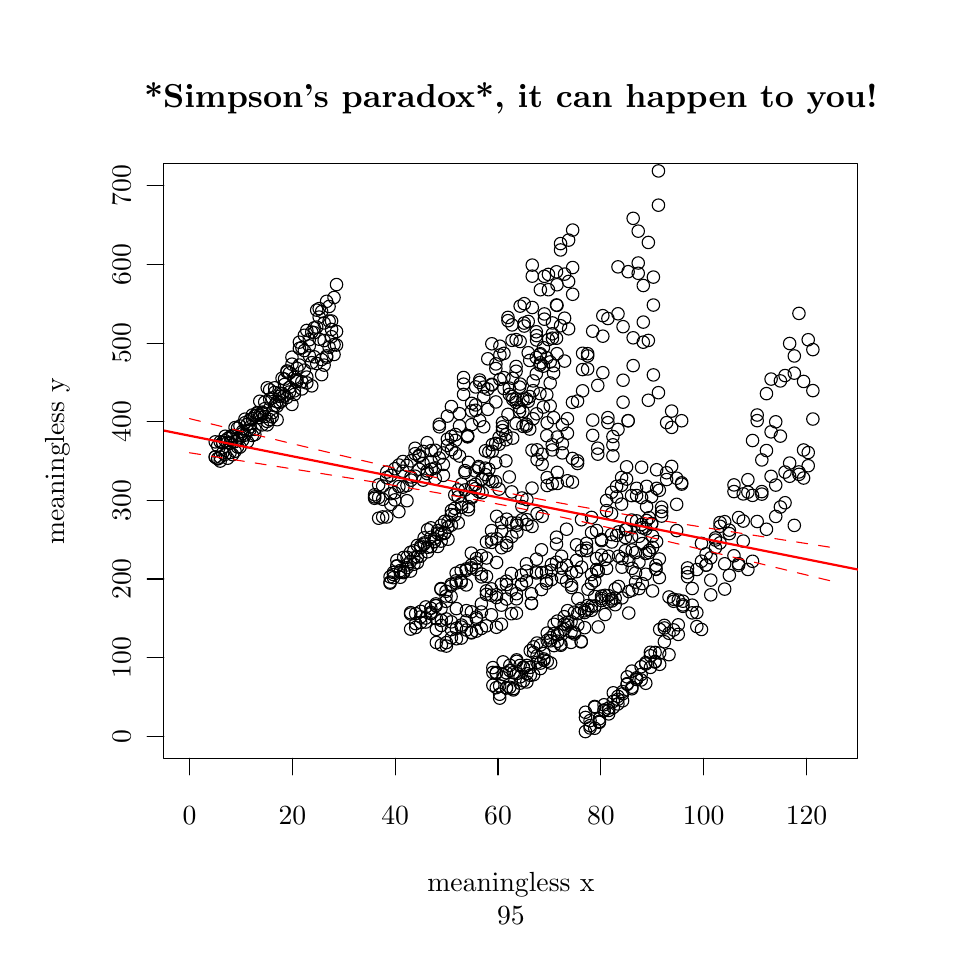
\begin{tikzpicture}[x=1pt,y=1pt]
\definecolor[named]{drawColor}{rgb}{0.00,0.00,0.00}
\definecolor[named]{fillColor}{rgb}{1.00,1.00,1.00}
\fill[color=fillColor,] (0,0) rectangle (325.21,325.21);
\begin{scope}
\path[clip] ( 49.20, 61.20) rectangle (300.01,276.01);
\definecolor[named]{drawColor}{rgb}{0.16,0.00,0.33}
\definecolor[named]{drawColor}{rgb}{0.00,0.00,0.00}

\draw[color=drawColor,line cap=round,line join=round,fill opacity=0.00,] ( 67.78,170.07) circle (  2.25);

\draw[color=drawColor,line cap=round,line join=round,fill opacity=0.00,] ( 68.67,169.52) circle (  2.25);

\draw[color=drawColor,line cap=round,line join=round,fill opacity=0.00,] ( 69.57,170.04) circle (  2.25);

\draw[color=drawColor,line cap=round,line join=round,fill opacity=0.00,] ( 70.46,171.54) circle (  2.25);

\draw[color=drawColor,line cap=round,line join=round,fill opacity=0.00,] ( 71.36,175.95) circle (  2.25);

\draw[color=drawColor,line cap=round,line join=round,fill opacity=0.00,] ( 72.25,176.72) circle (  2.25);

\draw[color=drawColor,line cap=round,line join=round,fill opacity=0.00,] ( 73.14,171.70) circle (  2.25);

\draw[color=drawColor,line cap=round,line join=round,fill opacity=0.00,] ( 74.04,177.81) circle (  2.25);

\draw[color=drawColor,line cap=round,line join=round,fill opacity=0.00,] ( 74.93,180.69) circle (  2.25);

\draw[color=drawColor,line cap=round,line join=round,fill opacity=0.00,] ( 75.83,176.29) circle (  2.25);

\draw[color=drawColor,line cap=round,line join=round,fill opacity=0.00,] ( 76.72,181.26) circle (  2.25);

\draw[color=drawColor,line cap=round,line join=round,fill opacity=0.00,] ( 77.62,178.55) circle (  2.25);

\draw[color=drawColor,line cap=round,line join=round,fill opacity=0.00,] ( 78.51,182.45) circle (  2.25);

\draw[color=drawColor,line cap=round,line join=round,fill opacity=0.00,] ( 79.40,181.91) circle (  2.25);

\draw[color=drawColor,line cap=round,line join=round,fill opacity=0.00,] ( 80.30,179.85) circle (  2.25);

\draw[color=drawColor,line cap=round,line join=round,fill opacity=0.00,] ( 81.19,185.24) circle (  2.25);

\draw[color=drawColor,line cap=round,line join=round,fill opacity=0.00,] ( 82.09,184.92) circle (  2.25);

\draw[color=drawColor,line cap=round,line join=round,fill opacity=0.00,] ( 82.98,185.23) circle (  2.25);

\draw[color=drawColor,line cap=round,line join=round,fill opacity=0.00,] ( 83.87,185.23) circle (  2.25);

\draw[color=drawColor,line cap=round,line join=round,fill opacity=0.00,] ( 84.77,186.27) circle (  2.25);

\draw[color=drawColor,line cap=round,line join=round,fill opacity=0.00,] ( 85.66,189.92) circle (  2.25);

\draw[color=drawColor,line cap=round,line join=round,fill opacity=0.00,] ( 86.56,195.08) circle (  2.25);

\draw[color=drawColor,line cap=round,line join=round,fill opacity=0.00,] ( 87.45,183.59) circle (  2.25);

\draw[color=drawColor,line cap=round,line join=round,fill opacity=0.00,] ( 88.35,191.36) circle (  2.25);

\draw[color=drawColor,line cap=round,line join=round,fill opacity=0.00,] ( 89.24,195.07) circle (  2.25);

\draw[color=drawColor,line cap=round,line join=round,fill opacity=0.00,] ( 90.13,188.45) circle (  2.25);

\draw[color=drawColor,line cap=round,line join=round,fill opacity=0.00,] ( 91.03,193.10) circle (  2.25);

\draw[color=drawColor,line cap=round,line join=round,fill opacity=0.00,] ( 91.92,198.51) circle (  2.25);

\draw[color=drawColor,line cap=round,line join=round,fill opacity=0.00,] ( 92.82,196.27) circle (  2.25);

\draw[color=drawColor,line cap=round,line join=round,fill opacity=0.00,] ( 93.71,191.59) circle (  2.25);

\draw[color=drawColor,line cap=round,line join=round,fill opacity=0.00,] ( 94.61,193.56) circle (  2.25);

\draw[color=drawColor,line cap=round,line join=round,fill opacity=0.00,] ( 95.50,206.14) circle (  2.25);

\draw[color=drawColor,line cap=round,line join=round,fill opacity=0.00,] ( 96.39,192.68) circle (  2.25);

\draw[color=drawColor,line cap=round,line join=round,fill opacity=0.00,] ( 97.29,197.94) circle (  2.25);

\draw[color=drawColor,line cap=round,line join=round,fill opacity=0.00,] ( 98.18,209.29) circle (  2.25);

\draw[color=drawColor,line cap=round,line join=round,fill opacity=0.00,] ( 99.08,194.66) circle (  2.25);

\draw[color=drawColor,line cap=round,line join=round,fill opacity=0.00,] ( 99.97,208.52) circle (  2.25);

\draw[color=drawColor,line cap=round,line join=round,fill opacity=0.00,] (100.86,198.95) circle (  2.25);

\draw[color=drawColor,line cap=round,line join=round,fill opacity=0.00,] (101.76,206.67) circle (  2.25);

\draw[color=drawColor,line cap=round,line join=round,fill opacity=0.00,] (102.65,195.77) circle (  2.25);

\draw[color=drawColor,line cap=round,line join=round,fill opacity=0.00,] (103.55,216.74) circle (  2.25);

\draw[color=drawColor,line cap=round,line join=round,fill opacity=0.00,] (104.44,223.15) circle (  2.25);

\draw[color=drawColor,line cap=round,line join=round,fill opacity=0.00,] (105.34,220.64) circle (  2.25);

\draw[color=drawColor,line cap=round,line join=round,fill opacity=0.00,] (106.23,205.27) circle (  2.25);

\draw[color=drawColor,line cap=round,line join=round,fill opacity=0.00,] (107.12,218.51) circle (  2.25);

\draw[color=drawColor,line cap=round,line join=round,fill opacity=0.00,] (108.02,206.09) circle (  2.25);

\draw[color=drawColor,line cap=round,line join=round,fill opacity=0.00,] (108.91,219.19) circle (  2.25);

\draw[color=drawColor,line cap=round,line join=round,fill opacity=0.00,] (109.81,213.53) circle (  2.25);

\draw[color=drawColor,line cap=round,line join=round,fill opacity=0.00,] (110.70,207.11) circle (  2.25);

\draw[color=drawColor,line cap=round,line join=round,fill opacity=0.00,] (111.60,210.53) circle (  2.25);

\draw[color=drawColor,line cap=round,line join=round,fill opacity=0.00,] ( 67.78,175.54) circle (  2.25);

\draw[color=drawColor,line cap=round,line join=round,fill opacity=0.00,] ( 68.67,174.10) circle (  2.25);

\draw[color=drawColor,line cap=round,line join=round,fill opacity=0.00,] ( 69.57,168.60) circle (  2.25);

\draw[color=drawColor,line cap=round,line join=round,fill opacity=0.00,] ( 70.46,175.23) circle (  2.25);

\draw[color=drawColor,line cap=round,line join=round,fill opacity=0.00,] ( 71.36,177.57) circle (  2.25);

\draw[color=drawColor,line cap=round,line join=round,fill opacity=0.00,] ( 72.25,175.36) circle (  2.25);

\draw[color=drawColor,line cap=round,line join=round,fill opacity=0.00,] ( 73.14,175.00) circle (  2.25);

\draw[color=drawColor,line cap=round,line join=round,fill opacity=0.00,] ( 74.04,177.58) circle (  2.25);

\draw[color=drawColor,line cap=round,line join=round,fill opacity=0.00,] ( 74.93,172.14) circle (  2.25);

\draw[color=drawColor,line cap=round,line join=round,fill opacity=0.00,] ( 75.83,173.71) circle (  2.25);

\draw[color=drawColor,line cap=round,line join=round,fill opacity=0.00,] ( 76.72,173.63) circle (  2.25);

\draw[color=drawColor,line cap=round,line join=round,fill opacity=0.00,] ( 77.62,179.32) circle (  2.25);

\draw[color=drawColor,line cap=round,line join=round,fill opacity=0.00,] ( 78.51,177.97) circle (  2.25);

\draw[color=drawColor,line cap=round,line join=round,fill opacity=0.00,] ( 79.40,175.60) circle (  2.25);

\draw[color=drawColor,line cap=round,line join=round,fill opacity=0.00,] ( 80.30,183.55) circle (  2.25);

\draw[color=drawColor,line cap=round,line join=round,fill opacity=0.00,] ( 81.19,177.85) circle (  2.25);

\draw[color=drawColor,line cap=round,line join=round,fill opacity=0.00,] ( 82.09,180.07) circle (  2.25);

\draw[color=drawColor,line cap=round,line join=round,fill opacity=0.00,] ( 82.98,186.14) circle (  2.25);

\draw[color=drawColor,line cap=round,line join=round,fill opacity=0.00,] ( 83.87,190.21) circle (  2.25);

\draw[color=drawColor,line cap=round,line join=round,fill opacity=0.00,] ( 84.77,185.80) circle (  2.25);

\draw[color=drawColor,line cap=round,line join=round,fill opacity=0.00,] ( 85.66,184.69) circle (  2.25);

\draw[color=drawColor,line cap=round,line join=round,fill opacity=0.00,] ( 86.56,181.69) circle (  2.25);

\draw[color=drawColor,line cap=round,line join=round,fill opacity=0.00,] ( 87.45,194.35) circle (  2.25);

\draw[color=drawColor,line cap=round,line join=round,fill opacity=0.00,] ( 88.35,184.59) circle (  2.25);

\draw[color=drawColor,line cap=round,line join=round,fill opacity=0.00,] ( 89.24,188.65) circle (  2.25);

\draw[color=drawColor,line cap=round,line join=round,fill opacity=0.00,] ( 90.13,183.54) circle (  2.25);

\draw[color=drawColor,line cap=round,line join=round,fill opacity=0.00,] ( 91.03,189.81) circle (  2.25);

\draw[color=drawColor,line cap=round,line join=round,fill opacity=0.00,] ( 91.92,193.02) circle (  2.25);

\draw[color=drawColor,line cap=round,line join=round,fill opacity=0.00,] ( 92.82,198.23) circle (  2.25);

\draw[color=drawColor,line cap=round,line join=round,fill opacity=0.00,] ( 93.71,201.16) circle (  2.25);

\draw[color=drawColor,line cap=round,line join=round,fill opacity=0.00,] ( 94.61,200.42) circle (  2.25);

\draw[color=drawColor,line cap=round,line join=round,fill opacity=0.00,] ( 95.50,189.06) circle (  2.25);

\draw[color=drawColor,line cap=round,line join=round,fill opacity=0.00,] ( 96.39,193.97) circle (  2.25);

\draw[color=drawColor,line cap=round,line join=round,fill opacity=0.00,] ( 97.29,197.34) circle (  2.25);

\draw[color=drawColor,line cap=round,line join=round,fill opacity=0.00,] ( 98.18,211.56) circle (  2.25);

\draw[color=drawColor,line cap=round,line join=round,fill opacity=0.00,] ( 99.08,197.24) circle (  2.25);

\draw[color=drawColor,line cap=round,line join=round,fill opacity=0.00,] ( 99.97,214.05) circle (  2.25);

\draw[color=drawColor,line cap=round,line join=round,fill opacity=0.00,] (100.86,215.81) circle (  2.25);

\draw[color=drawColor,line cap=round,line join=round,fill opacity=0.00,] (101.76,212.45) circle (  2.25);

\draw[color=drawColor,line cap=round,line join=round,fill opacity=0.00,] (102.65,215.21) circle (  2.25);

\draw[color=drawColor,line cap=round,line join=round,fill opacity=0.00,] (103.55,206.27) circle (  2.25);

\draw[color=drawColor,line cap=round,line join=round,fill opacity=0.00,] (104.44,203.85) circle (  2.25);

\draw[color=drawColor,line cap=round,line join=round,fill opacity=0.00,] (105.34,212.64) circle (  2.25);

\draw[color=drawColor,line cap=round,line join=round,fill opacity=0.00,] (106.23,199.82) circle (  2.25);

\draw[color=drawColor,line cap=round,line join=round,fill opacity=0.00,] (107.12,212.15) circle (  2.25);

\draw[color=drawColor,line cap=round,line join=round,fill opacity=0.00,] (108.02,226.32) circle (  2.25);

\draw[color=drawColor,line cap=round,line join=round,fill opacity=0.00,] (108.91,224.45) circle (  2.25);

\draw[color=drawColor,line cap=round,line join=round,fill opacity=0.00,] (109.81,216.16) circle (  2.25);

\draw[color=drawColor,line cap=round,line join=round,fill opacity=0.00,] (110.70,227.70) circle (  2.25);

\draw[color=drawColor,line cap=round,line join=round,fill opacity=0.00,] (111.60,215.41) circle (  2.25);

\draw[color=drawColor,line cap=round,line join=round,fill opacity=0.00,] ( 67.78,170.07) circle (  2.25);

\draw[color=drawColor,line cap=round,line join=round,fill opacity=0.00,] ( 68.67,169.40) circle (  2.25);

\draw[color=drawColor,line cap=round,line join=round,fill opacity=0.00,] ( 69.57,175.55) circle (  2.25);

\draw[color=drawColor,line cap=round,line join=round,fill opacity=0.00,] ( 70.46,175.35) circle (  2.25);

\draw[color=drawColor,line cap=round,line join=round,fill opacity=0.00,] ( 71.36,171.02) circle (  2.25);

\draw[color=drawColor,line cap=round,line join=round,fill opacity=0.00,] ( 72.25,169.64) circle (  2.25);

\draw[color=drawColor,line cap=round,line join=round,fill opacity=0.00,] ( 73.14,177.35) circle (  2.25);

\draw[color=drawColor,line cap=round,line join=round,fill opacity=0.00,] ( 74.04,170.91) circle (  2.25);

\draw[color=drawColor,line cap=round,line join=round,fill opacity=0.00,] ( 74.93,175.63) circle (  2.25);

\draw[color=drawColor,line cap=round,line join=round,fill opacity=0.00,] ( 75.83,180.48) circle (  2.25);

\draw[color=drawColor,line cap=round,line join=round,fill opacity=0.00,] ( 76.72,177.29) circle (  2.25);

\draw[color=drawColor,line cap=round,line join=round,fill opacity=0.00,] ( 77.62,176.08) circle (  2.25);

\draw[color=drawColor,line cap=round,line join=round,fill opacity=0.00,] ( 78.51,183.73) circle (  2.25);

\draw[color=drawColor,line cap=round,line join=round,fill opacity=0.00,] ( 79.40,179.65) circle (  2.25);

\draw[color=drawColor,line cap=round,line join=round,fill opacity=0.00,] ( 80.30,180.93) circle (  2.25);

\draw[color=drawColor,line cap=round,line join=round,fill opacity=0.00,] ( 81.19,183.94) circle (  2.25);

\draw[color=drawColor,line cap=round,line join=round,fill opacity=0.00,] ( 82.09,178.21) circle (  2.25);

\draw[color=drawColor,line cap=round,line join=round,fill opacity=0.00,] ( 82.98,185.91) circle (  2.25);

\draw[color=drawColor,line cap=round,line join=round,fill opacity=0.00,] ( 83.87,184.35) circle (  2.25);

\draw[color=drawColor,line cap=round,line join=round,fill opacity=0.00,] ( 84.77,181.69) circle (  2.25);

\draw[color=drawColor,line cap=round,line join=round,fill opacity=0.00,] ( 85.66,187.52) circle (  2.25);

\draw[color=drawColor,line cap=round,line join=round,fill opacity=0.00,] ( 86.56,182.93) circle (  2.25);

\draw[color=drawColor,line cap=round,line join=round,fill opacity=0.00,] ( 87.45,190.97) circle (  2.25);

\draw[color=drawColor,line cap=round,line join=round,fill opacity=0.00,] ( 88.35,186.04) circle (  2.25);

\draw[color=drawColor,line cap=round,line join=round,fill opacity=0.00,] ( 89.24,193.40) circle (  2.25);

\draw[color=drawColor,line cap=round,line join=round,fill opacity=0.00,] ( 90.13,190.07) circle (  2.25);

\draw[color=drawColor,line cap=round,line join=round,fill opacity=0.00,] ( 91.03,192.01) circle (  2.25);

\draw[color=drawColor,line cap=round,line join=round,fill opacity=0.00,] ( 91.92,190.34) circle (  2.25);

\draw[color=drawColor,line cap=round,line join=round,fill opacity=0.00,] ( 92.82,192.18) circle (  2.25);

\draw[color=drawColor,line cap=round,line join=round,fill opacity=0.00,] ( 93.71,200.78) circle (  2.25);

\draw[color=drawColor,line cap=round,line join=round,fill opacity=0.00,] ( 94.61,195.23) circle (  2.25);

\draw[color=drawColor,line cap=round,line join=round,fill opacity=0.00,] ( 95.50,203.62) circle (  2.25);

\draw[color=drawColor,line cap=round,line join=round,fill opacity=0.00,] ( 96.39,198.81) circle (  2.25);

\draw[color=drawColor,line cap=round,line join=round,fill opacity=0.00,] ( 97.29,202.13) circle (  2.25);

\draw[color=drawColor,line cap=round,line join=round,fill opacity=0.00,] ( 98.18,203.30) circle (  2.25);

\draw[color=drawColor,line cap=round,line join=round,fill opacity=0.00,] ( 99.08,209.61) circle (  2.25);

\draw[color=drawColor,line cap=round,line join=round,fill opacity=0.00,] ( 99.97,201.46) circle (  2.25);

\draw[color=drawColor,line cap=round,line join=round,fill opacity=0.00,] (100.86,196.83) circle (  2.25);

\draw[color=drawColor,line cap=round,line join=round,fill opacity=0.00,] (101.76,210.24) circle (  2.25);

\draw[color=drawColor,line cap=round,line join=round,fill opacity=0.00,] (102.65,204.15) circle (  2.25);

\draw[color=drawColor,line cap=round,line join=round,fill opacity=0.00,] (103.55,215.00) circle (  2.25);

\draw[color=drawColor,line cap=round,line join=round,fill opacity=0.00,] (104.44,217.01) circle (  2.25);

\draw[color=drawColor,line cap=round,line join=round,fill opacity=0.00,] (105.34,223.69) circle (  2.25);

\draw[color=drawColor,line cap=round,line join=round,fill opacity=0.00,] (106.23,222.64) circle (  2.25);

\draw[color=drawColor,line cap=round,line join=round,fill opacity=0.00,] (107.12,203.27) circle (  2.25);

\draw[color=drawColor,line cap=round,line join=round,fill opacity=0.00,] (108.02,206.61) circle (  2.25);

\draw[color=drawColor,line cap=round,line join=round,fill opacity=0.00,] (108.91,209.73) circle (  2.25);

\draw[color=drawColor,line cap=round,line join=round,fill opacity=0.00,] (109.81,219.21) circle (  2.25);

\draw[color=drawColor,line cap=round,line join=round,fill opacity=0.00,] (110.70,210.70) circle (  2.25);

\draw[color=drawColor,line cap=round,line join=round,fill opacity=0.00,] (111.60,232.38) circle (  2.25);

\draw[color=drawColor,line cap=round,line join=round,fill opacity=0.00,] (125.37,155.16) circle (  2.25);

\draw[color=drawColor,line cap=round,line join=round,fill opacity=0.00,] (126.83,159.99) circle (  2.25);

\draw[color=drawColor,line cap=round,line join=round,fill opacity=0.00,] (128.29,159.59) circle (  2.25);

\draw[color=drawColor,line cap=round,line join=round,fill opacity=0.00,] (129.75,148.39) circle (  2.25);

\draw[color=drawColor,line cap=round,line join=round,fill opacity=0.00,] (131.21,163.44) circle (  2.25);

\draw[color=drawColor,line cap=round,line join=round,fill opacity=0.00,] (132.68,154.58) circle (  2.25);

\draw[color=drawColor,line cap=round,line join=round,fill opacity=0.00,] (134.14,150.31) circle (  2.25);

\draw[color=drawColor,line cap=round,line join=round,fill opacity=0.00,] (135.60,164.93) circle (  2.25);

\draw[color=drawColor,line cap=round,line join=round,fill opacity=0.00,] (137.06,154.27) circle (  2.25);

\draw[color=drawColor,line cap=round,line join=round,fill opacity=0.00,] (138.52,162.86) circle (  2.25);

\draw[color=drawColor,line cap=round,line join=round,fill opacity=0.00,] (139.98,171.25) circle (  2.25);

\draw[color=drawColor,line cap=round,line join=round,fill opacity=0.00,] (141.44,170.30) circle (  2.25);

\draw[color=drawColor,line cap=round,line join=round,fill opacity=0.00,] (142.90,167.74) circle (  2.25);

\draw[color=drawColor,line cap=round,line join=round,fill opacity=0.00,] (144.36,175.26) circle (  2.25);

\draw[color=drawColor,line cap=round,line join=round,fill opacity=0.00,] (145.82,165.65) circle (  2.25);

\draw[color=drawColor,line cap=round,line join=round,fill opacity=0.00,] (147.28,162.24) circle (  2.25);

\draw[color=drawColor,line cap=round,line join=round,fill opacity=0.00,] (148.74,180.98) circle (  2.25);

\draw[color=drawColor,line cap=round,line join=round,fill opacity=0.00,] (150.20,163.42) circle (  2.25);

\draw[color=drawColor,line cap=round,line join=round,fill opacity=0.00,] (151.66,176.50) circle (  2.25);

\draw[color=drawColor,line cap=round,line join=round,fill opacity=0.00,] (153.12,177.49) circle (  2.25);

\draw[color=drawColor,line cap=round,line join=round,fill opacity=0.00,] (154.58,176.08) circle (  2.25);

\draw[color=drawColor,line cap=round,line join=round,fill opacity=0.00,] (156.04,185.71) circle (  2.25);

\draw[color=drawColor,line cap=round,line join=round,fill opacity=0.00,] (157.50,196.39) circle (  2.25);

\draw[color=drawColor,line cap=round,line join=round,fill opacity=0.00,] (158.96,177.37) circle (  2.25);

\draw[color=drawColor,line cap=round,line join=round,fill opacity=0.00,] (160.42,181.74) circle (  2.25);

\draw[color=drawColor,line cap=round,line join=round,fill opacity=0.00,] (161.88,186.95) circle (  2.25);

\draw[color=drawColor,line cap=round,line join=round,fill opacity=0.00,] (163.34,183.23) circle (  2.25);

\draw[color=drawColor,line cap=round,line join=round,fill opacity=0.00,] (164.80,195.31) circle (  2.25);

\draw[color=drawColor,line cap=round,line join=round,fill opacity=0.00,] (166.26,187.28) circle (  2.25);

\draw[color=drawColor,line cap=round,line join=round,fill opacity=0.00,] (167.72,210.98) circle (  2.25);

\draw[color=drawColor,line cap=round,line join=round,fill opacity=0.00,] (169.18,189.96) circle (  2.25);

\draw[color=drawColor,line cap=round,line join=round,fill opacity=0.00,] (170.64,206.93) circle (  2.25);

\draw[color=drawColor,line cap=round,line join=round,fill opacity=0.00,] (172.10,207.52) circle (  2.25);

\draw[color=drawColor,line cap=round,line join=round,fill opacity=0.00,] (173.56,220.51) circle (  2.25);

\draw[color=drawColor,line cap=round,line join=round,fill opacity=0.00,] (175.02,191.97) circle (  2.25);

\draw[color=drawColor,line cap=round,line join=round,fill opacity=0.00,] (176.49,202.78) circle (  2.25);

\draw[color=drawColor,line cap=round,line join=round,fill opacity=0.00,] (177.95,211.80) circle (  2.25);

\draw[color=drawColor,line cap=round,line join=round,fill opacity=0.00,] (179.41,225.48) circle (  2.25);

\draw[color=drawColor,line cap=round,line join=round,fill opacity=0.00,] (180.87,207.75) circle (  2.25);

\draw[color=drawColor,line cap=round,line join=round,fill opacity=0.00,] (182.33,235.42) circle (  2.25);

\draw[color=drawColor,line cap=round,line join=round,fill opacity=0.00,] (183.79,206.00) circle (  2.25);

\draw[color=drawColor,line cap=round,line join=round,fill opacity=0.00,] (185.25,207.39) circle (  2.25);

\draw[color=drawColor,line cap=round,line join=round,fill opacity=0.00,] (186.71,219.88) circle (  2.25);

\draw[color=drawColor,line cap=round,line join=round,fill opacity=0.00,] (188.17,212.49) circle (  2.25);

\draw[color=drawColor,line cap=round,line join=round,fill opacity=0.00,] (189.63,213.00) circle (  2.25);

\draw[color=drawColor,line cap=round,line join=round,fill opacity=0.00,] (191.09,225.01) circle (  2.25);

\draw[color=drawColor,line cap=round,line join=round,fill opacity=0.00,] (192.55,244.88) circle (  2.25);

\draw[color=drawColor,line cap=round,line join=round,fill opacity=0.00,] (194.01,220.23) circle (  2.25);

\draw[color=drawColor,line cap=round,line join=round,fill opacity=0.00,] (195.47,248.45) circle (  2.25);

\draw[color=drawColor,line cap=round,line join=round,fill opacity=0.00,] (196.93,228.87) circle (  2.25);

\draw[color=drawColor,line cap=round,line join=round,fill opacity=0.00,] (125.37,156.42) circle (  2.25);

\draw[color=drawColor,line cap=round,line join=round,fill opacity=0.00,] (126.83,147.95) circle (  2.25);

\draw[color=drawColor,line cap=round,line join=round,fill opacity=0.00,] (128.29,154.79) circle (  2.25);

\draw[color=drawColor,line cap=round,line join=round,fill opacity=0.00,] (129.75,162.62) circle (  2.25);

\draw[color=drawColor,line cap=round,line join=round,fill opacity=0.00,] (131.21,152.97) circle (  2.25);

\draw[color=drawColor,line cap=round,line join=round,fill opacity=0.00,] (132.68,165.83) circle (  2.25);

\draw[color=drawColor,line cap=round,line join=round,fill opacity=0.00,] (134.14,159.38) circle (  2.25);

\draw[color=drawColor,line cap=round,line join=round,fill opacity=0.00,] (135.60,168.44) circle (  2.25);

\draw[color=drawColor,line cap=round,line join=round,fill opacity=0.00,] (137.06,159.79) circle (  2.25);

\draw[color=drawColor,line cap=round,line join=round,fill opacity=0.00,] (138.52,168.67) circle (  2.25);

\draw[color=drawColor,line cap=round,line join=round,fill opacity=0.00,] (139.98,163.14) circle (  2.25);

\draw[color=drawColor,line cap=round,line join=round,fill opacity=0.00,] (141.44,170.67) circle (  2.25);

\draw[color=drawColor,line cap=round,line join=round,fill opacity=0.00,] (142.90,172.07) circle (  2.25);

\draw[color=drawColor,line cap=round,line join=round,fill opacity=0.00,] (144.36,164.09) circle (  2.25);

\draw[color=drawColor,line cap=round,line join=round,fill opacity=0.00,] (145.82,172.40) circle (  2.25);

\draw[color=drawColor,line cap=round,line join=round,fill opacity=0.00,] (147.28,166.10) circle (  2.25);

\draw[color=drawColor,line cap=round,line join=round,fill opacity=0.00,] (148.74,181.90) circle (  2.25);

\draw[color=drawColor,line cap=round,line join=round,fill opacity=0.00,] (150.20,167.38) circle (  2.25);

\draw[color=drawColor,line cap=round,line join=round,fill opacity=0.00,] (151.66,174.23) circle (  2.25);

\draw[color=drawColor,line cap=round,line join=round,fill opacity=0.00,] (153.12,188.30) circle (  2.25);

\draw[color=drawColor,line cap=round,line join=round,fill opacity=0.00,] (154.58,178.19) circle (  2.25);

\draw[color=drawColor,line cap=round,line join=round,fill opacity=0.00,] (156.04,181.30) circle (  2.25);

\draw[color=drawColor,line cap=round,line join=round,fill opacity=0.00,] (157.50,192.69) circle (  2.25);

\draw[color=drawColor,line cap=round,line join=round,fill opacity=0.00,] (158.96,177.85) circle (  2.25);

\draw[color=drawColor,line cap=round,line join=round,fill opacity=0.00,] (160.42,189.46) circle (  2.25);

\draw[color=drawColor,line cap=round,line join=round,fill opacity=0.00,] (161.88,188.89) circle (  2.25);

\draw[color=drawColor,line cap=round,line join=round,fill opacity=0.00,] (163.34,197.02) circle (  2.25);

\draw[color=drawColor,line cap=round,line join=round,fill opacity=0.00,] (164.80,180.98) circle (  2.25);

\draw[color=drawColor,line cap=round,line join=round,fill opacity=0.00,] (166.26,205.56) circle (  2.25);

\draw[color=drawColor,line cap=round,line join=round,fill opacity=0.00,] (167.72,196.10) circle (  2.25);

\draw[color=drawColor,line cap=round,line join=round,fill opacity=0.00,] (169.18,203.69) circle (  2.25);

\draw[color=drawColor,line cap=round,line join=round,fill opacity=0.00,] (170.64,210.10) circle (  2.25);

\draw[color=drawColor,line cap=round,line join=round,fill opacity=0.00,] (172.10,194.83) circle (  2.25);

\draw[color=drawColor,line cap=round,line join=round,fill opacity=0.00,] (173.56,219.33) circle (  2.25);

\draw[color=drawColor,line cap=round,line join=round,fill opacity=0.00,] (175.02,217.80) circle (  2.25);

\draw[color=drawColor,line cap=round,line join=round,fill opacity=0.00,] (176.49,212.48) circle (  2.25);

\draw[color=drawColor,line cap=round,line join=round,fill opacity=0.00,] (177.95,196.42) circle (  2.25);

\draw[color=drawColor,line cap=round,line join=round,fill opacity=0.00,] (179.41,218.47) circle (  2.25);

\draw[color=drawColor,line cap=round,line join=round,fill opacity=0.00,] (180.87,219.04) circle (  2.25);

\draw[color=drawColor,line cap=round,line join=round,fill opacity=0.00,] (182.33,239.41) circle (  2.25);

\draw[color=drawColor,line cap=round,line join=round,fill opacity=0.00,] (183.79,200.13) circle (  2.25);

\draw[color=drawColor,line cap=round,line join=round,fill opacity=0.00,] (185.25,230.51) circle (  2.25);

\draw[color=drawColor,line cap=round,line join=round,fill opacity=0.00,] (186.71,235.36) circle (  2.25);

\draw[color=drawColor,line cap=round,line join=round,fill opacity=0.00,] (188.17,230.52) circle (  2.25);

\draw[color=drawColor,line cap=round,line join=round,fill opacity=0.00,] (189.63,218.51) circle (  2.25);

\draw[color=drawColor,line cap=round,line join=round,fill opacity=0.00,] (191.09,236.99) circle (  2.25);

\draw[color=drawColor,line cap=round,line join=round,fill opacity=0.00,] (192.55,247.18) circle (  2.25);

\draw[color=drawColor,line cap=round,line join=round,fill opacity=0.00,] (194.01,236.16) circle (  2.25);

\draw[color=drawColor,line cap=round,line join=round,fill opacity=0.00,] (195.47,216.39) circle (  2.25);

\draw[color=drawColor,line cap=round,line join=round,fill opacity=0.00,] (196.93,238.53) circle (  2.25);

\draw[color=drawColor,line cap=round,line join=round,fill opacity=0.00,] (125.37,155.66) circle (  2.25);

\draw[color=drawColor,line cap=round,line join=round,fill opacity=0.00,] (126.83,155.45) circle (  2.25);

\draw[color=drawColor,line cap=round,line join=round,fill opacity=0.00,] (128.29,148.41) circle (  2.25);

\draw[color=drawColor,line cap=round,line join=round,fill opacity=0.00,] (129.75,164.62) circle (  2.25);

\draw[color=drawColor,line cap=round,line join=round,fill opacity=0.00,] (131.21,156.82) circle (  2.25);

\draw[color=drawColor,line cap=round,line join=round,fill opacity=0.00,] (132.68,157.14) circle (  2.25);

\draw[color=drawColor,line cap=round,line join=round,fill opacity=0.00,] (134.14,167.17) circle (  2.25);

\draw[color=drawColor,line cap=round,line join=round,fill opacity=0.00,] (135.60,159.18) circle (  2.25);

\draw[color=drawColor,line cap=round,line join=round,fill opacity=0.00,] (137.06,167.04) circle (  2.25);

\draw[color=drawColor,line cap=round,line join=round,fill opacity=0.00,] (138.52,161.72) circle (  2.25);

\draw[color=drawColor,line cap=round,line join=round,fill opacity=0.00,] (139.98,173.23) circle (  2.25);

\draw[color=drawColor,line cap=round,line join=round,fill opacity=0.00,] (141.44,165.64) circle (  2.25);

\draw[color=drawColor,line cap=round,line join=round,fill opacity=0.00,] (142.90,161.71) circle (  2.25);

\draw[color=drawColor,line cap=round,line join=round,fill opacity=0.00,] (144.36,165.06) circle (  2.25);

\draw[color=drawColor,line cap=round,line join=round,fill opacity=0.00,] (145.82,168.31) circle (  2.25);

\draw[color=drawColor,line cap=round,line join=round,fill opacity=0.00,] (147.28,172.50) circle (  2.25);

\draw[color=drawColor,line cap=round,line join=round,fill opacity=0.00,] (148.74,169.68) circle (  2.25);

\draw[color=drawColor,line cap=round,line join=round,fill opacity=0.00,] (150.20,171.52) circle (  2.25);

\draw[color=drawColor,line cap=round,line join=round,fill opacity=0.00,] (151.66,184.84) circle (  2.25);

\draw[color=drawColor,line cap=round,line join=round,fill opacity=0.00,] (153.12,172.76) circle (  2.25);

\draw[color=drawColor,line cap=round,line join=round,fill opacity=0.00,] (154.58,171.46) circle (  2.25);

\draw[color=drawColor,line cap=round,line join=round,fill opacity=0.00,] (156.04,170.41) circle (  2.25);

\draw[color=drawColor,line cap=round,line join=round,fill opacity=0.00,] (157.50,198.79) circle (  2.25);

\draw[color=drawColor,line cap=round,line join=round,fill opacity=0.00,] (158.96,177.45) circle (  2.25);

\draw[color=drawColor,line cap=round,line join=round,fill opacity=0.00,] (160.42,186.70) circle (  2.25);

\draw[color=drawColor,line cap=round,line join=round,fill opacity=0.00,] (161.88,195.38) circle (  2.25);

\draw[color=drawColor,line cap=round,line join=round,fill opacity=0.00,] (163.34,197.89) circle (  2.25);

\draw[color=drawColor,line cap=round,line join=round,fill opacity=0.00,] (164.80,191.93) circle (  2.25);

\draw[color=drawColor,line cap=round,line join=round,fill opacity=0.00,] (166.26,194.59) circle (  2.25);

\draw[color=drawColor,line cap=round,line join=round,fill opacity=0.00,] (167.72,196.34) circle (  2.25);

\draw[color=drawColor,line cap=round,line join=round,fill opacity=0.00,] (169.18,202.03) circle (  2.25);

\draw[color=drawColor,line cap=round,line join=round,fill opacity=0.00,] (170.64,198.15) circle (  2.25);

\draw[color=drawColor,line cap=round,line join=round,fill opacity=0.00,] (172.10,198.73) circle (  2.25);

\draw[color=drawColor,line cap=round,line join=round,fill opacity=0.00,] (173.56,185.48) circle (  2.25);

\draw[color=drawColor,line cap=round,line join=round,fill opacity=0.00,] (175.02,212.23) circle (  2.25);

\draw[color=drawColor,line cap=round,line join=round,fill opacity=0.00,] (176.49,201.05) circle (  2.25);

\draw[color=drawColor,line cap=round,line join=round,fill opacity=0.00,] (177.95,224.59) circle (  2.25);

\draw[color=drawColor,line cap=round,line join=round,fill opacity=0.00,] (179.41,217.39) circle (  2.25);

\draw[color=drawColor,line cap=round,line join=round,fill opacity=0.00,] (180.87,190.19) circle (  2.25);

\draw[color=drawColor,line cap=round,line join=round,fill opacity=0.00,] (182.33,224.09) circle (  2.25);

\draw[color=drawColor,line cap=round,line join=round,fill opacity=0.00,] (183.79,215.32) circle (  2.25);

\draw[color=drawColor,line cap=round,line join=round,fill opacity=0.00,] (185.25,204.09) circle (  2.25);

\draw[color=drawColor,line cap=round,line join=round,fill opacity=0.00,] (186.71,221.77) circle (  2.25);

\draw[color=drawColor,line cap=round,line join=round,fill opacity=0.00,] (188.17,236.06) circle (  2.25);

\draw[color=drawColor,line cap=round,line join=round,fill opacity=0.00,] (189.63,214.59) circle (  2.25);

\draw[color=drawColor,line cap=round,line join=round,fill opacity=0.00,] (191.09,212.99) circle (  2.25);

\draw[color=drawColor,line cap=round,line join=round,fill opacity=0.00,] (192.55,217.49) circle (  2.25);

\draw[color=drawColor,line cap=round,line join=round,fill opacity=0.00,] (194.01,204.73) circle (  2.25);

\draw[color=drawColor,line cap=round,line join=round,fill opacity=0.00,] (195.47,233.50) circle (  2.25);

\draw[color=drawColor,line cap=round,line join=round,fill opacity=0.00,] (196.93,252.07) circle (  2.25);

\draw[color=drawColor,line cap=round,line join=round,fill opacity=0.00,] (130.95,124.86) circle (  2.25);

\draw[color=drawColor,line cap=round,line join=round,fill opacity=0.00,] (132.18,126.47) circle (  2.25);

\draw[color=drawColor,line cap=round,line join=round,fill opacity=0.00,] (133.41,132.75) circle (  2.25);

\draw[color=drawColor,line cap=round,line join=round,fill opacity=0.00,] (134.64,128.40) circle (  2.25);

\draw[color=drawColor,line cap=round,line join=round,fill opacity=0.00,] (135.87,133.79) circle (  2.25);

\draw[color=drawColor,line cap=round,line join=round,fill opacity=0.00,] (137.10,133.82) circle (  2.25);

\draw[color=drawColor,line cap=round,line join=round,fill opacity=0.00,] (138.33,135.62) circle (  2.25);

\draw[color=drawColor,line cap=round,line join=round,fill opacity=0.00,] (139.56,133.64) circle (  2.25);

\draw[color=drawColor,line cap=round,line join=round,fill opacity=0.00,] (140.80,138.11) circle (  2.25);

\draw[color=drawColor,line cap=round,line join=round,fill opacity=0.00,] (142.03,137.92) circle (  2.25);

\draw[color=drawColor,line cap=round,line join=round,fill opacity=0.00,] (143.26,139.02) circle (  2.25);

\draw[color=drawColor,line cap=round,line join=round,fill opacity=0.00,] (144.49,135.82) circle (  2.25);

\draw[color=drawColor,line cap=round,line join=round,fill opacity=0.00,] (145.72,144.47) circle (  2.25);

\draw[color=drawColor,line cap=round,line join=round,fill opacity=0.00,] (146.95,140.53) circle (  2.25);

\draw[color=drawColor,line cap=round,line join=round,fill opacity=0.00,] (148.18,142.52) circle (  2.25);

\draw[color=drawColor,line cap=round,line join=round,fill opacity=0.00,] (149.41,145.40) circle (  2.25);

\draw[color=drawColor,line cap=round,line join=round,fill opacity=0.00,] (150.64,142.45) circle (  2.25);

\draw[color=drawColor,line cap=round,line join=round,fill opacity=0.00,] (151.88,146.66) circle (  2.25);

\draw[color=drawColor,line cap=round,line join=round,fill opacity=0.00,] (153.11,149.26) circle (  2.25);

\draw[color=drawColor,line cap=round,line join=round,fill opacity=0.00,] (154.34,151.50) circle (  2.25);

\draw[color=drawColor,line cap=round,line join=round,fill opacity=0.00,] (155.57,158.18) circle (  2.25);

\draw[color=drawColor,line cap=round,line join=round,fill opacity=0.00,] (156.80,153.18) circle (  2.25);

\draw[color=drawColor,line cap=round,line join=round,fill opacity=0.00,] (158.03,164.44) circle (  2.25);

\draw[color=drawColor,line cap=round,line join=round,fill opacity=0.00,] (159.26,168.12) circle (  2.25);

\draw[color=drawColor,line cap=round,line join=round,fill opacity=0.00,] (160.49,159.48) circle (  2.25);

\draw[color=drawColor,line cap=round,line join=round,fill opacity=0.00,] (161.72,160.17) circle (  2.25);

\draw[color=drawColor,line cap=round,line join=round,fill opacity=0.00,] (162.96,157.59) circle (  2.25);

\draw[color=drawColor,line cap=round,line join=round,fill opacity=0.00,] (164.19,161.99) circle (  2.25);

\draw[color=drawColor,line cap=round,line join=round,fill opacity=0.00,] (165.42,172.32) circle (  2.25);

\draw[color=drawColor,line cap=round,line join=round,fill opacity=0.00,] (166.65,165.64) circle (  2.25);

\draw[color=drawColor,line cap=round,line join=round,fill opacity=0.00,] (167.88,172.13) circle (  2.25);

\draw[color=drawColor,line cap=round,line join=round,fill opacity=0.00,] (169.11,168.03) circle (  2.25);

\draw[color=drawColor,line cap=round,line join=round,fill opacity=0.00,] (170.34,177.12) circle (  2.25);

\draw[color=drawColor,line cap=round,line join=round,fill opacity=0.00,] (171.57,179.63) circle (  2.25);

\draw[color=drawColor,line cap=round,line join=round,fill opacity=0.00,] (172.80,178.16) circle (  2.25);

\draw[color=drawColor,line cap=round,line join=round,fill opacity=0.00,] (174.03,194.97) circle (  2.25);

\draw[color=drawColor,line cap=round,line join=round,fill opacity=0.00,] (175.27,198.51) circle (  2.25);

\draw[color=drawColor,line cap=round,line join=round,fill opacity=0.00,] (176.50,182.16) circle (  2.25);

\draw[color=drawColor,line cap=round,line join=round,fill opacity=0.00,] (177.73,186.50) circle (  2.25);

\draw[color=drawColor,line cap=round,line join=round,fill opacity=0.00,] (178.96,186.47) circle (  2.25);

\draw[color=drawColor,line cap=round,line join=round,fill opacity=0.00,] (180.19,181.22) circle (  2.25);

\draw[color=drawColor,line cap=round,line join=round,fill opacity=0.00,] (181.42,180.16) circle (  2.25);

\draw[color=drawColor,line cap=round,line join=round,fill opacity=0.00,] (182.65,194.02) circle (  2.25);

\draw[color=drawColor,line cap=round,line join=round,fill opacity=0.00,] (183.88,185.67) circle (  2.25);

\draw[color=drawColor,line cap=round,line join=round,fill opacity=0.00,] (185.11,192.98) circle (  2.25);

\draw[color=drawColor,line cap=round,line join=round,fill opacity=0.00,] (186.35,202.91) circle (  2.25);

\draw[color=drawColor,line cap=round,line join=round,fill opacity=0.00,] (187.58,192.58) circle (  2.25);

\draw[color=drawColor,line cap=round,line join=round,fill opacity=0.00,] (188.81,196.81) circle (  2.25);

\draw[color=drawColor,line cap=round,line join=round,fill opacity=0.00,] (190.04,184.29) circle (  2.25);

\draw[color=drawColor,line cap=round,line join=round,fill opacity=0.00,] (191.27,207.41) circle (  2.25);

\draw[color=drawColor,line cap=round,line join=round,fill opacity=0.00,] (130.95,124.52) circle (  2.25);

\draw[color=drawColor,line cap=round,line join=round,fill opacity=0.00,] (132.18,128.36) circle (  2.25);

\draw[color=drawColor,line cap=round,line join=round,fill opacity=0.00,] (133.41,130.58) circle (  2.25);

\draw[color=drawColor,line cap=round,line join=round,fill opacity=0.00,] (134.64,126.62) circle (  2.25);

\draw[color=drawColor,line cap=round,line join=round,fill opacity=0.00,] (135.87,128.68) circle (  2.25);

\draw[color=drawColor,line cap=round,line join=round,fill opacity=0.00,] (137.10,130.08) circle (  2.25);

\draw[color=drawColor,line cap=round,line join=round,fill opacity=0.00,] (138.33,132.37) circle (  2.25);

\draw[color=drawColor,line cap=round,line join=round,fill opacity=0.00,] (139.56,131.32) circle (  2.25);

\draw[color=drawColor,line cap=round,line join=round,fill opacity=0.00,] (140.80,133.97) circle (  2.25);

\draw[color=drawColor,line cap=round,line join=round,fill opacity=0.00,] (142.03,134.23) circle (  2.25);

\draw[color=drawColor,line cap=round,line join=round,fill opacity=0.00,] (143.26,138.58) circle (  2.25);

\draw[color=drawColor,line cap=round,line join=round,fill opacity=0.00,] (144.49,143.79) circle (  2.25);

\draw[color=drawColor,line cap=round,line join=round,fill opacity=0.00,] (145.72,137.68) circle (  2.25);

\draw[color=drawColor,line cap=round,line join=round,fill opacity=0.00,] (146.95,139.53) circle (  2.25);

\draw[color=drawColor,line cap=round,line join=round,fill opacity=0.00,] (148.18,137.75) circle (  2.25);

\draw[color=drawColor,line cap=round,line join=round,fill opacity=0.00,] (149.41,142.23) circle (  2.25);

\draw[color=drawColor,line cap=round,line join=round,fill opacity=0.00,] (150.64,146.79) circle (  2.25);

\draw[color=drawColor,line cap=round,line join=round,fill opacity=0.00,] (151.88,144.71) circle (  2.25);

\draw[color=drawColor,line cap=round,line join=round,fill opacity=0.00,] (153.11,145.46) circle (  2.25);

\draw[color=drawColor,line cap=round,line join=round,fill opacity=0.00,] (154.34,156.37) circle (  2.25);

\draw[color=drawColor,line cap=round,line join=round,fill opacity=0.00,] (155.57,155.65) circle (  2.25);

\draw[color=drawColor,line cap=round,line join=round,fill opacity=0.00,] (156.80,151.89) circle (  2.25);

\draw[color=drawColor,line cap=round,line join=round,fill opacity=0.00,] (158.03,165.13) circle (  2.25);

\draw[color=drawColor,line cap=round,line join=round,fill opacity=0.00,] (159.26,152.14) circle (  2.25);

\draw[color=drawColor,line cap=round,line join=round,fill opacity=0.00,] (160.49,155.34) circle (  2.25);

\draw[color=drawColor,line cap=round,line join=round,fill opacity=0.00,] (161.72,165.03) circle (  2.25);

\draw[color=drawColor,line cap=round,line join=round,fill opacity=0.00,] (162.96,166.14) circle (  2.25);

\draw[color=drawColor,line cap=round,line join=round,fill opacity=0.00,] (164.19,162.14) circle (  2.25);

\draw[color=drawColor,line cap=round,line join=round,fill opacity=0.00,] (165.42,166.03) circle (  2.25);

\draw[color=drawColor,line cap=round,line join=round,fill opacity=0.00,] (166.65,171.89) circle (  2.25);

\draw[color=drawColor,line cap=round,line join=round,fill opacity=0.00,] (167.88,161.19) circle (  2.25);

\draw[color=drawColor,line cap=round,line join=round,fill opacity=0.00,] (169.11,161.14) circle (  2.25);

\draw[color=drawColor,line cap=round,line join=round,fill opacity=0.00,] (170.34,174.69) circle (  2.25);

\draw[color=drawColor,line cap=round,line join=round,fill opacity=0.00,] (171.57,180.96) circle (  2.25);

\draw[color=drawColor,line cap=round,line join=round,fill opacity=0.00,] (172.80,176.29) circle (  2.25);

\draw[color=drawColor,line cap=round,line join=round,fill opacity=0.00,] (174.03,192.70) circle (  2.25);

\draw[color=drawColor,line cap=round,line join=round,fill opacity=0.00,] (175.27,176.90) circle (  2.25);

\draw[color=drawColor,line cap=round,line join=round,fill opacity=0.00,] (176.50,189.83) circle (  2.25);

\draw[color=drawColor,line cap=round,line join=round,fill opacity=0.00,] (177.73,195.33) circle (  2.25);

\draw[color=drawColor,line cap=round,line join=round,fill opacity=0.00,] (178.96,190.80) circle (  2.25);

\draw[color=drawColor,line cap=round,line join=round,fill opacity=0.00,] (180.19,181.90) circle (  2.25);

\draw[color=drawColor,line cap=round,line join=round,fill opacity=0.00,] (181.42,204.95) circle (  2.25);

\draw[color=drawColor,line cap=round,line join=round,fill opacity=0.00,] (182.65,183.89) circle (  2.25);

\draw[color=drawColor,line cap=round,line join=round,fill opacity=0.00,] (183.88,212.35) circle (  2.25);

\draw[color=drawColor,line cap=round,line join=round,fill opacity=0.00,] (185.11,207.01) circle (  2.25);

\draw[color=drawColor,line cap=round,line join=round,fill opacity=0.00,] (186.35,209.59) circle (  2.25);

\draw[color=drawColor,line cap=round,line join=round,fill opacity=0.00,] (187.58,177.77) circle (  2.25);

\draw[color=drawColor,line cap=round,line join=round,fill opacity=0.00,] (188.81,204.43) circle (  2.25);

\draw[color=drawColor,line cap=round,line join=round,fill opacity=0.00,] (190.04,203.06) circle (  2.25);

\draw[color=drawColor,line cap=round,line join=round,fill opacity=0.00,] (191.27,224.88) circle (  2.25);

\draw[color=drawColor,line cap=round,line join=round,fill opacity=0.00,] (130.95,126.77) circle (  2.25);

\draw[color=drawColor,line cap=round,line join=round,fill opacity=0.00,] (132.18,127.59) circle (  2.25);

\draw[color=drawColor,line cap=round,line join=round,fill opacity=0.00,] (133.41,130.75) circle (  2.25);

\draw[color=drawColor,line cap=round,line join=round,fill opacity=0.00,] (134.64,129.04) circle (  2.25);

\draw[color=drawColor,line cap=round,line join=round,fill opacity=0.00,] (135.87,128.28) circle (  2.25);

\draw[color=drawColor,line cap=round,line join=round,fill opacity=0.00,] (137.10,131.05) circle (  2.25);

\draw[color=drawColor,line cap=round,line join=round,fill opacity=0.00,] (138.33,128.84) circle (  2.25);

\draw[color=drawColor,line cap=round,line join=round,fill opacity=0.00,] (139.56,136.14) circle (  2.25);

\draw[color=drawColor,line cap=round,line join=round,fill opacity=0.00,] (140.80,131.90) circle (  2.25);

\draw[color=drawColor,line cap=round,line join=round,fill opacity=0.00,] (142.03,137.34) circle (  2.25);

\draw[color=drawColor,line cap=round,line join=round,fill opacity=0.00,] (143.26,140.85) circle (  2.25);

\draw[color=drawColor,line cap=round,line join=round,fill opacity=0.00,] (144.49,137.47) circle (  2.25);

\draw[color=drawColor,line cap=round,line join=round,fill opacity=0.00,] (145.72,141.07) circle (  2.25);

\draw[color=drawColor,line cap=round,line join=round,fill opacity=0.00,] (146.95,139.49) circle (  2.25);

\draw[color=drawColor,line cap=round,line join=round,fill opacity=0.00,] (148.18,143.48) circle (  2.25);

\draw[color=drawColor,line cap=round,line join=round,fill opacity=0.00,] (149.41,139.68) circle (  2.25);

\draw[color=drawColor,line cap=round,line join=round,fill opacity=0.00,] (150.64,142.70) circle (  2.25);

\draw[color=drawColor,line cap=round,line join=round,fill opacity=0.00,] (151.88,140.38) circle (  2.25);

\draw[color=drawColor,line cap=round,line join=round,fill opacity=0.00,] (153.11,150.72) circle (  2.25);

\draw[color=drawColor,line cap=round,line join=round,fill opacity=0.00,] (154.34,149.11) circle (  2.25);

\draw[color=drawColor,line cap=round,line join=round,fill opacity=0.00,] (155.57,146.29) circle (  2.25);

\draw[color=drawColor,line cap=round,line join=round,fill opacity=0.00,] (156.80,160.30) circle (  2.25);

\draw[color=drawColor,line cap=round,line join=round,fill opacity=0.00,] (158.03,158.16) circle (  2.25);

\draw[color=drawColor,line cap=round,line join=round,fill opacity=0.00,] (159.26,150.98) circle (  2.25);

\draw[color=drawColor,line cap=round,line join=round,fill opacity=0.00,] (160.49,155.74) circle (  2.25);

\draw[color=drawColor,line cap=round,line join=round,fill opacity=0.00,] (161.72,158.63) circle (  2.25);

\draw[color=drawColor,line cap=round,line join=round,fill opacity=0.00,] (162.96,166.64) circle (  2.25);

\draw[color=drawColor,line cap=round,line join=round,fill opacity=0.00,] (164.19,157.18) circle (  2.25);

\draw[color=drawColor,line cap=round,line join=round,fill opacity=0.00,] (165.42,163.69) circle (  2.25);

\draw[color=drawColor,line cap=round,line join=round,fill opacity=0.00,] (166.65,162.01) circle (  2.25);

\draw[color=drawColor,line cap=round,line join=round,fill opacity=0.00,] (167.88,174.54) circle (  2.25);

\draw[color=drawColor,line cap=round,line join=round,fill opacity=0.00,] (169.11,174.99) circle (  2.25);

\draw[color=drawColor,line cap=round,line join=round,fill opacity=0.00,] (170.34,158.48) circle (  2.25);

\draw[color=drawColor,line cap=round,line join=round,fill opacity=0.00,] (171.57,182.46) circle (  2.25);

\draw[color=drawColor,line cap=round,line join=round,fill opacity=0.00,] (172.80,168.68) circle (  2.25);

\draw[color=drawColor,line cap=round,line join=round,fill opacity=0.00,] (174.03,162.86) circle (  2.25);

\draw[color=drawColor,line cap=round,line join=round,fill opacity=0.00,] (175.27,190.91) circle (  2.25);

\draw[color=drawColor,line cap=round,line join=round,fill opacity=0.00,] (176.50,190.99) circle (  2.25);

\draw[color=drawColor,line cap=round,line join=round,fill opacity=0.00,] (177.73,187.91) circle (  2.25);

\draw[color=drawColor,line cap=round,line join=round,fill opacity=0.00,] (178.96,181.16) circle (  2.25);

\draw[color=drawColor,line cap=round,line join=round,fill opacity=0.00,] (180.19,191.09) circle (  2.25);

\draw[color=drawColor,line cap=round,line join=round,fill opacity=0.00,] (181.42,191.91) circle (  2.25);

\draw[color=drawColor,line cap=round,line join=round,fill opacity=0.00,] (182.65,197.56) circle (  2.25);

\draw[color=drawColor,line cap=round,line join=round,fill opacity=0.00,] (183.88,213.93) circle (  2.25);

\draw[color=drawColor,line cap=round,line join=round,fill opacity=0.00,] (185.11,203.31) circle (  2.25);

\draw[color=drawColor,line cap=round,line join=round,fill opacity=0.00,] (186.35,188.12) circle (  2.25);

\draw[color=drawColor,line cap=round,line join=round,fill opacity=0.00,] (187.58,205.94) circle (  2.25);

\draw[color=drawColor,line cap=round,line join=round,fill opacity=0.00,] (188.81,188.56) circle (  2.25);

\draw[color=drawColor,line cap=round,line join=round,fill opacity=0.00,] (190.04,200.41) circle (  2.25);

\draw[color=drawColor,line cap=round,line join=round,fill opacity=0.00,] (191.27,232.31) circle (  2.25);

\draw[color=drawColor,line cap=round,line join=round,fill opacity=0.00,] (138.38,113.82) circle (  2.25);

\draw[color=drawColor,line cap=round,line join=round,fill opacity=0.00,] (140.21,108.46) circle (  2.25);

\draw[color=drawColor,line cap=round,line join=round,fill opacity=0.00,] (142.03,110.25) circle (  2.25);

\draw[color=drawColor,line cap=round,line join=round,fill opacity=0.00,] (143.86,111.88) circle (  2.25);

\draw[color=drawColor,line cap=round,line join=round,fill opacity=0.00,] (145.69,113.43) circle (  2.25);

\draw[color=drawColor,line cap=round,line join=round,fill opacity=0.00,] (147.52,116.36) circle (  2.25);

\draw[color=drawColor,line cap=round,line join=round,fill opacity=0.00,] (149.34,122.27) circle (  2.25);

\draw[color=drawColor,line cap=round,line join=round,fill opacity=0.00,] (151.17,117.91) circle (  2.25);

\draw[color=drawColor,line cap=round,line join=round,fill opacity=0.00,] (153.00,124.07) circle (  2.25);

\draw[color=drawColor,line cap=round,line join=round,fill opacity=0.00,] (154.83,128.10) circle (  2.25);

\draw[color=drawColor,line cap=round,line join=round,fill opacity=0.00,] (156.65,129.03) circle (  2.25);

\draw[color=drawColor,line cap=round,line join=round,fill opacity=0.00,] (158.48,129.62) circle (  2.25);

\draw[color=drawColor,line cap=round,line join=round,fill opacity=0.00,] (160.31,135.34) circle (  2.25);

\draw[color=drawColor,line cap=round,line join=round,fill opacity=0.00,] (162.14,129.37) circle (  2.25);

\draw[color=drawColor,line cap=round,line join=round,fill opacity=0.00,] (163.97,134.47) circle (  2.25);

\draw[color=drawColor,line cap=round,line join=round,fill opacity=0.00,] (165.79,126.92) circle (  2.25);

\draw[color=drawColor,line cap=round,line join=round,fill opacity=0.00,] (167.62,140.36) circle (  2.25);

\draw[color=drawColor,line cap=round,line join=round,fill opacity=0.00,] (169.45,148.63) circle (  2.25);

\draw[color=drawColor,line cap=round,line join=round,fill opacity=0.00,] (171.28,146.27) circle (  2.25);

\draw[color=drawColor,line cap=round,line join=round,fill opacity=0.00,] (173.10,139.16) circle (  2.25);

\draw[color=drawColor,line cap=round,line join=round,fill opacity=0.00,] (174.93,141.31) circle (  2.25);

\draw[color=drawColor,line cap=round,line join=round,fill opacity=0.00,] (176.76,146.20) circle (  2.25);

\draw[color=drawColor,line cap=round,line join=round,fill opacity=0.00,] (178.59,155.25) circle (  2.25);

\draw[color=drawColor,line cap=round,line join=round,fill opacity=0.00,] (180.41,147.42) circle (  2.25);

\draw[color=drawColor,line cap=round,line join=round,fill opacity=0.00,] (182.24,172.52) circle (  2.25);

\draw[color=drawColor,line cap=round,line join=round,fill opacity=0.00,] (184.07,149.61) circle (  2.25);

\draw[color=drawColor,line cap=round,line join=round,fill opacity=0.00,] (185.90,148.64) circle (  2.25);

\draw[color=drawColor,line cap=round,line join=round,fill opacity=0.00,] (187.72,159.77) circle (  2.25);

\draw[color=drawColor,line cap=round,line join=round,fill opacity=0.00,] (189.55,160.40) circle (  2.25);

\draw[color=drawColor,line cap=round,line join=round,fill opacity=0.00,] (191.38,177.29) circle (  2.25);

\draw[color=drawColor,line cap=round,line join=round,fill opacity=0.00,] (193.21,181.75) circle (  2.25);

\draw[color=drawColor,line cap=round,line join=round,fill opacity=0.00,] (195.04,161.48) circle (  2.25);

\draw[color=drawColor,line cap=round,line join=round,fill opacity=0.00,] (196.86,169.55) circle (  2.25);

\draw[color=drawColor,line cap=round,line join=round,fill opacity=0.00,] (198.69,168.67) circle (  2.25);

\draw[color=drawColor,line cap=round,line join=round,fill opacity=0.00,] (200.52,193.98) circle (  2.25);

\draw[color=drawColor,line cap=round,line join=round,fill opacity=0.00,] (202.35,201.88) circle (  2.25);

\draw[color=drawColor,line cap=round,line join=round,fill opacity=0.00,] (204.17,177.90) circle (  2.25);

\draw[color=drawColor,line cap=round,line join=round,fill opacity=0.00,] (206.00,171.11) circle (  2.25);

\draw[color=drawColor,line cap=round,line join=round,fill opacity=0.00,] (207.83,200.54) circle (  2.25);

\draw[color=drawColor,line cap=round,line join=round,fill opacity=0.00,] (209.66,182.48) circle (  2.25);

\draw[color=drawColor,line cap=round,line join=round,fill opacity=0.00,] (211.48,170.50) circle (  2.25);

\draw[color=drawColor,line cap=round,line join=round,fill opacity=0.00,] (213.31,180.02) circle (  2.25);

\draw[color=drawColor,line cap=round,line join=round,fill opacity=0.00,] (215.14,217.16) circle (  2.25);

\draw[color=drawColor,line cap=round,line join=round,fill opacity=0.00,] (216.97,183.20) circle (  2.25);

\draw[color=drawColor,line cap=round,line join=round,fill opacity=0.00,] (218.79,203.09) circle (  2.25);

\draw[color=drawColor,line cap=round,line join=round,fill opacity=0.00,] (220.62,240.17) circle (  2.25);

\draw[color=drawColor,line cap=round,line join=round,fill opacity=0.00,] (222.45,211.56) circle (  2.25);

\draw[color=drawColor,line cap=round,line join=round,fill opacity=0.00,] (224.28,190.57) circle (  2.25);

\draw[color=drawColor,line cap=round,line join=round,fill opacity=0.00,] (226.10,224.98) circle (  2.25);

\draw[color=drawColor,line cap=round,line join=round,fill opacity=0.00,] (227.93,273.44) circle (  2.25);

\draw[color=drawColor,line cap=round,line join=round,fill opacity=0.00,] (138.38,113.33) circle (  2.25);

\draw[color=drawColor,line cap=round,line join=round,fill opacity=0.00,] (140.21,113.46) circle (  2.25);

\draw[color=drawColor,line cap=round,line join=round,fill opacity=0.00,] (142.03,114.27) circle (  2.25);

\draw[color=drawColor,line cap=round,line join=round,fill opacity=0.00,] (143.86,110.44) circle (  2.25);

\draw[color=drawColor,line cap=round,line join=round,fill opacity=0.00,] (145.69,115.39) circle (  2.25);

\draw[color=drawColor,line cap=round,line join=round,fill opacity=0.00,] (147.52,116.98) circle (  2.25);

\draw[color=drawColor,line cap=round,line join=round,fill opacity=0.00,] (149.34,122.53) circle (  2.25);

\draw[color=drawColor,line cap=round,line join=round,fill opacity=0.00,] (151.17,121.55) circle (  2.25);

\draw[color=drawColor,line cap=round,line join=round,fill opacity=0.00,] (153.00,119.66) circle (  2.25);

\draw[color=drawColor,line cap=round,line join=round,fill opacity=0.00,] (154.83,125.33) circle (  2.25);

\draw[color=drawColor,line cap=round,line join=round,fill opacity=0.00,] (156.65,125.36) circle (  2.25);

\draw[color=drawColor,line cap=round,line join=round,fill opacity=0.00,] (158.48,123.84) circle (  2.25);

\draw[color=drawColor,line cap=round,line join=round,fill opacity=0.00,] (160.31,130.04) circle (  2.25);

\draw[color=drawColor,line cap=round,line join=round,fill opacity=0.00,] (162.14,131.88) circle (  2.25);

\draw[color=drawColor,line cap=round,line join=round,fill opacity=0.00,] (163.97,126.76) circle (  2.25);

\draw[color=drawColor,line cap=round,line join=round,fill opacity=0.00,] (165.79,133.58) circle (  2.25);

\draw[color=drawColor,line cap=round,line join=round,fill opacity=0.00,] (167.62,139.21) circle (  2.25);

\draw[color=drawColor,line cap=round,line join=round,fill opacity=0.00,] (169.45,140.56) circle (  2.25);

\draw[color=drawColor,line cap=round,line join=round,fill opacity=0.00,] (171.28,143.23) circle (  2.25);

\draw[color=drawColor,line cap=round,line join=round,fill opacity=0.00,] (173.10,138.08) circle (  2.25);

\draw[color=drawColor,line cap=round,line join=round,fill opacity=0.00,] (174.93,146.29) circle (  2.25);

\draw[color=drawColor,line cap=round,line join=round,fill opacity=0.00,] (176.76,142.95) circle (  2.25);

\draw[color=drawColor,line cap=round,line join=round,fill opacity=0.00,] (178.59,152.19) circle (  2.25);

\draw[color=drawColor,line cap=round,line join=round,fill opacity=0.00,] (180.41,145.71) circle (  2.25);

\draw[color=drawColor,line cap=round,line join=round,fill opacity=0.00,] (182.24,158.83) circle (  2.25);

\draw[color=drawColor,line cap=round,line join=round,fill opacity=0.00,] (184.07,169.09) circle (  2.25);

\draw[color=drawColor,line cap=round,line join=round,fill opacity=0.00,] (185.90,167.45) circle (  2.25);

\draw[color=drawColor,line cap=round,line join=round,fill opacity=0.00,] (187.72,162.63) circle (  2.25);

\draw[color=drawColor,line cap=round,line join=round,fill opacity=0.00,] (189.55,172.62) circle (  2.25);

\draw[color=drawColor,line cap=round,line join=round,fill opacity=0.00,] (191.38,160.51) circle (  2.25);

\draw[color=drawColor,line cap=round,line join=round,fill opacity=0.00,] (193.21,171.55) circle (  2.25);

\draw[color=drawColor,line cap=round,line join=round,fill opacity=0.00,] (195.04,178.66) circle (  2.25);

\draw[color=drawColor,line cap=round,line join=round,fill opacity=0.00,] (196.86,189.81) circle (  2.25);

\draw[color=drawColor,line cap=round,line join=round,fill opacity=0.00,] (198.69,190.29) circle (  2.25);

\draw[color=drawColor,line cap=round,line join=round,fill opacity=0.00,] (200.52,201.66) circle (  2.25);

\draw[color=drawColor,line cap=round,line join=round,fill opacity=0.00,] (202.35,207.40) circle (  2.25);

\draw[color=drawColor,line cap=round,line join=round,fill opacity=0.00,] (204.17,183.42) circle (  2.25);

\draw[color=drawColor,line cap=round,line join=round,fill opacity=0.00,] (206.00,195.95) circle (  2.25);

\draw[color=drawColor,line cap=round,line join=round,fill opacity=0.00,] (207.83,221.14) circle (  2.25);

\draw[color=drawColor,line cap=round,line join=round,fill opacity=0.00,] (209.66,220.11) circle (  2.25);

\draw[color=drawColor,line cap=round,line join=round,fill opacity=0.00,] (211.48,174.47) circle (  2.25);

\draw[color=drawColor,line cap=round,line join=round,fill opacity=0.00,] (213.31,221.82) circle (  2.25);

\draw[color=drawColor,line cap=round,line join=round,fill opacity=0.00,] (215.14,189.88) circle (  2.25);

\draw[color=drawColor,line cap=round,line join=round,fill opacity=0.00,] (216.97,237.03) circle (  2.25);

\draw[color=drawColor,line cap=round,line join=round,fill opacity=0.00,] (218.79,213.14) circle (  2.25);

\draw[color=drawColor,line cap=round,line join=round,fill opacity=0.00,] (220.62,251.68) circle (  2.25);

\draw[color=drawColor,line cap=round,line join=round,fill opacity=0.00,] (222.45,218.82) circle (  2.25);

\draw[color=drawColor,line cap=round,line join=round,fill opacity=0.00,] (224.28,212.19) circle (  2.25);

\draw[color=drawColor,line cap=round,line join=round,fill opacity=0.00,] (226.10,235.08) circle (  2.25);

\draw[color=drawColor,line cap=round,line join=round,fill opacity=0.00,] (227.93,261.07) circle (  2.25);

\draw[color=drawColor,line cap=round,line join=round,fill opacity=0.00,] (138.38,107.88) circle (  2.25);

\draw[color=drawColor,line cap=round,line join=round,fill opacity=0.00,] (140.21,109.86) circle (  2.25);

\draw[color=drawColor,line cap=round,line join=round,fill opacity=0.00,] (142.03,112.28) circle (  2.25);

\draw[color=drawColor,line cap=round,line join=round,fill opacity=0.00,] (143.86,115.89) circle (  2.25);

\draw[color=drawColor,line cap=round,line join=round,fill opacity=0.00,] (145.69,113.93) circle (  2.25);

\draw[color=drawColor,line cap=round,line join=round,fill opacity=0.00,] (147.52,116.37) circle (  2.25);

\draw[color=drawColor,line cap=round,line join=round,fill opacity=0.00,] (149.34,115.25) circle (  2.25);

\draw[color=drawColor,line cap=round,line join=round,fill opacity=0.00,] (151.17,119.83) circle (  2.25);

\draw[color=drawColor,line cap=round,line join=round,fill opacity=0.00,] (153.00,123.44) circle (  2.25);

\draw[color=drawColor,line cap=round,line join=round,fill opacity=0.00,] (154.83,124.54) circle (  2.25);

\draw[color=drawColor,line cap=round,line join=round,fill opacity=0.00,] (156.65,124.79) circle (  2.25);

\draw[color=drawColor,line cap=round,line join=round,fill opacity=0.00,] (158.48,129.12) circle (  2.25);

\draw[color=drawColor,line cap=round,line join=round,fill opacity=0.00,] (160.31,130.97) circle (  2.25);

\draw[color=drawColor,line cap=round,line join=round,fill opacity=0.00,] (162.14,133.42) circle (  2.25);

\draw[color=drawColor,line cap=round,line join=round,fill opacity=0.00,] (163.97,127.77) circle (  2.25);

\draw[color=drawColor,line cap=round,line join=round,fill opacity=0.00,] (165.79,139.36) circle (  2.25);

\draw[color=drawColor,line cap=round,line join=round,fill opacity=0.00,] (167.62,143.47) circle (  2.25);

\draw[color=drawColor,line cap=round,line join=round,fill opacity=0.00,] (169.45,131.95) circle (  2.25);

\draw[color=drawColor,line cap=round,line join=round,fill opacity=0.00,] (171.28,137.28) circle (  2.25);

\draw[color=drawColor,line cap=round,line join=round,fill opacity=0.00,] (173.10,147.60) circle (  2.25);

\draw[color=drawColor,line cap=round,line join=round,fill opacity=0.00,] (174.93,157.46) circle (  2.25);

\draw[color=drawColor,line cap=round,line join=round,fill opacity=0.00,] (176.76,145.42) circle (  2.25);

\draw[color=drawColor,line cap=round,line join=round,fill opacity=0.00,] (178.59,147.35) circle (  2.25);

\draw[color=drawColor,line cap=round,line join=round,fill opacity=0.00,] (180.41,154.68) circle (  2.25);

\draw[color=drawColor,line cap=round,line join=round,fill opacity=0.00,] (182.24,144.97) circle (  2.25);

\draw[color=drawColor,line cap=round,line join=round,fill opacity=0.00,] (184.07,172.65) circle (  2.25);

\draw[color=drawColor,line cap=round,line join=round,fill opacity=0.00,] (185.90,171.07) circle (  2.25);

\draw[color=drawColor,line cap=round,line join=round,fill opacity=0.00,] (187.72,182.44) circle (  2.25);

\draw[color=drawColor,line cap=round,line join=round,fill opacity=0.00,] (189.55,174.50) circle (  2.25);

\draw[color=drawColor,line cap=round,line join=round,fill opacity=0.00,] (191.38,164.52) circle (  2.25);

\draw[color=drawColor,line cap=round,line join=round,fill opacity=0.00,] (193.21,174.88) circle (  2.25);

\draw[color=drawColor,line cap=round,line join=round,fill opacity=0.00,] (195.04,183.92) circle (  2.25);

\draw[color=drawColor,line cap=round,line join=round,fill opacity=0.00,] (196.86,161.00) circle (  2.25);

\draw[color=drawColor,line cap=round,line join=round,fill opacity=0.00,] (198.69,167.72) circle (  2.25);

\draw[color=drawColor,line cap=round,line join=round,fill opacity=0.00,] (200.52,207.55) circle (  2.25);

\draw[color=drawColor,line cap=round,line join=round,fill opacity=0.00,] (202.35,206.60) circle (  2.25);

\draw[color=drawColor,line cap=round,line join=round,fill opacity=0.00,] (204.17,215.53) circle (  2.25);

\draw[color=drawColor,line cap=round,line join=round,fill opacity=0.00,] (206.00,173.25) circle (  2.25);

\draw[color=drawColor,line cap=round,line join=round,fill opacity=0.00,] (207.83,213.73) circle (  2.25);

\draw[color=drawColor,line cap=round,line join=round,fill opacity=0.00,] (209.66,184.30) circle (  2.25);

\draw[color=drawColor,line cap=round,line join=round,fill opacity=0.00,] (211.48,177.46) circle (  2.25);

\draw[color=drawColor,line cap=round,line join=round,fill opacity=0.00,] (213.31,238.78) circle (  2.25);

\draw[color=drawColor,line cap=round,line join=round,fill opacity=0.00,] (215.14,197.82) circle (  2.25);

\draw[color=drawColor,line cap=round,line join=round,fill opacity=0.00,] (216.97,183.14) circle (  2.25);

\draw[color=drawColor,line cap=round,line join=round,fill opacity=0.00,] (218.79,256.31) circle (  2.25);

\draw[color=drawColor,line cap=round,line join=round,fill opacity=0.00,] (220.62,236.45) circle (  2.25);

\draw[color=drawColor,line cap=round,line join=round,fill opacity=0.00,] (222.45,232.04) circle (  2.25);

\draw[color=drawColor,line cap=round,line join=round,fill opacity=0.00,] (224.28,247.60) circle (  2.25);

\draw[color=drawColor,line cap=round,line join=round,fill opacity=0.00,] (226.10,199.73) circle (  2.25);

\draw[color=drawColor,line cap=round,line join=round,fill opacity=0.00,] (227.93,193.31) circle (  2.25);

\draw[color=drawColor,line cap=round,line join=round,fill opacity=0.00,] (147.67,107.76) circle (  2.25);

\draw[color=drawColor,line cap=round,line join=round,fill opacity=0.00,] (149.48,109.20) circle (  2.25);

\draw[color=drawColor,line cap=round,line join=round,fill opacity=0.00,] (151.29,101.75) circle (  2.25);

\draw[color=drawColor,line cap=round,line join=round,fill opacity=0.00,] (153.10,104.75) circle (  2.25);

\draw[color=drawColor,line cap=round,line join=round,fill opacity=0.00,] (154.90,108.14) circle (  2.25);

\draw[color=drawColor,line cap=round,line join=round,fill opacity=0.00,] (156.71,104.65) circle (  2.25);

\draw[color=drawColor,line cap=round,line join=round,fill opacity=0.00,] (158.52,110.89) circle (  2.25);

\draw[color=drawColor,line cap=round,line join=round,fill opacity=0.00,] (160.33,106.50) circle (  2.25);

\draw[color=drawColor,line cap=round,line join=round,fill opacity=0.00,] (162.14,107.15) circle (  2.25);

\draw[color=drawColor,line cap=round,line join=round,fill opacity=0.00,] (163.95,117.02) circle (  2.25);

\draw[color=drawColor,line cap=round,line join=round,fill opacity=0.00,] (165.76,109.05) circle (  2.25);

\draw[color=drawColor,line cap=round,line join=round,fill opacity=0.00,] (167.57,113.05) circle (  2.25);

\draw[color=drawColor,line cap=round,line join=round,fill opacity=0.00,] (169.38,108.55) circle (  2.25);

\draw[color=drawColor,line cap=round,line join=round,fill opacity=0.00,] (171.19,116.54) circle (  2.25);

\draw[color=drawColor,line cap=round,line join=round,fill opacity=0.00,] (173.00,118.75) circle (  2.25);

\draw[color=drawColor,line cap=round,line join=round,fill opacity=0.00,] (174.81,121.98) circle (  2.25);

\draw[color=drawColor,line cap=round,line join=round,fill opacity=0.00,] (176.61,120.67) circle (  2.25);

\draw[color=drawColor,line cap=round,line join=round,fill opacity=0.00,] (178.42,127.37) circle (  2.25);

\draw[color=drawColor,line cap=round,line join=round,fill opacity=0.00,] (180.23,128.86) circle (  2.25);

\draw[color=drawColor,line cap=round,line join=round,fill opacity=0.00,] (182.04,117.12) circle (  2.25);

\draw[color=drawColor,line cap=round,line join=round,fill opacity=0.00,] (183.85,133.16) circle (  2.25);

\draw[color=drawColor,line cap=round,line join=round,fill opacity=0.00,] (185.66,122.18) circle (  2.25);

\draw[color=drawColor,line cap=round,line join=round,fill opacity=0.00,] (187.47,125.37) circle (  2.25);

\draw[color=drawColor,line cap=round,line join=round,fill opacity=0.00,] (189.28,129.15) circle (  2.25);

\draw[color=drawColor,line cap=round,line join=round,fill opacity=0.00,] (191.09,138.62) circle (  2.25);

\draw[color=drawColor,line cap=round,line join=round,fill opacity=0.00,] (192.90,129.90) circle (  2.25);

\draw[color=drawColor,line cap=round,line join=round,fill opacity=0.00,] (194.71,125.15) circle (  2.25);

\draw[color=drawColor,line cap=round,line join=round,fill opacity=0.00,] (196.52,122.89) circle (  2.25);

\draw[color=drawColor,line cap=round,line join=round,fill opacity=0.00,] (198.32,138.34) circle (  2.25);

\draw[color=drawColor,line cap=round,line join=round,fill opacity=0.00,] (200.13,130.26) circle (  2.25);

\draw[color=drawColor,line cap=round,line join=round,fill opacity=0.00,] (201.94,137.12) circle (  2.25);

\draw[color=drawColor,line cap=round,line join=round,fill opacity=0.00,] (203.75,127.63) circle (  2.25);

\draw[color=drawColor,line cap=round,line join=round,fill opacity=0.00,] (205.56,133.41) circle (  2.25);

\draw[color=drawColor,line cap=round,line join=round,fill opacity=0.00,] (207.37,134.62) circle (  2.25);

\draw[color=drawColor,line cap=round,line join=round,fill opacity=0.00,] (209.18,154.37) circle (  2.25);

\draw[color=drawColor,line cap=round,line join=round,fill opacity=0.00,] (210.99,142.03) circle (  2.25);

\draw[color=drawColor,line cap=round,line join=round,fill opacity=0.00,] (212.80,159.43) circle (  2.25);

\draw[color=drawColor,line cap=round,line join=round,fill opacity=0.00,] (214.61,153.05) circle (  2.25);

\draw[color=drawColor,line cap=round,line join=round,fill opacity=0.00,] (216.42,143.90) circle (  2.25);

\draw[color=drawColor,line cap=round,line join=round,fill opacity=0.00,] (218.22,156.12) circle (  2.25);

\draw[color=drawColor,line cap=round,line join=round,fill opacity=0.00,] (220.03,146.98) circle (  2.25);

\draw[color=drawColor,line cap=round,line join=round,fill opacity=0.00,] (221.84,155.37) circle (  2.25);

\draw[color=drawColor,line cap=round,line join=round,fill opacity=0.00,] (223.65,159.47) circle (  2.25);

\draw[color=drawColor,line cap=round,line join=round,fill opacity=0.00,] (225.46,155.72) circle (  2.25);

\draw[color=drawColor,line cap=round,line join=round,fill opacity=0.00,] (227.27,139.50) circle (  2.25);

\draw[color=drawColor,line cap=round,line join=round,fill opacity=0.00,] (229.08,150.33) circle (  2.25);

\draw[color=drawColor,line cap=round,line join=round,fill opacity=0.00,] (230.89,161.93) circle (  2.25);

\draw[color=drawColor,line cap=round,line join=round,fill opacity=0.00,] (232.70,180.77) circle (  2.25);

\draw[color=drawColor,line cap=round,line join=round,fill opacity=0.00,] (234.51,162.40) circle (  2.25);

\draw[color=drawColor,line cap=round,line join=round,fill opacity=0.00,] (236.32,160.74) circle (  2.25);

\draw[color=drawColor,line cap=round,line join=round,fill opacity=0.00,] (147.67,111.68) circle (  2.25);

\draw[color=drawColor,line cap=round,line join=round,fill opacity=0.00,] (149.48,111.03) circle (  2.25);

\draw[color=drawColor,line cap=round,line join=round,fill opacity=0.00,] (151.29,103.01) circle (  2.25);

\draw[color=drawColor,line cap=round,line join=round,fill opacity=0.00,] (153.10,110.49) circle (  2.25);

\draw[color=drawColor,line cap=round,line join=round,fill opacity=0.00,] (154.90,104.40) circle (  2.25);

\draw[color=drawColor,line cap=round,line join=round,fill opacity=0.00,] (156.71,109.35) circle (  2.25);

\draw[color=drawColor,line cap=round,line join=round,fill opacity=0.00,] (158.52,107.55) circle (  2.25);

\draw[color=drawColor,line cap=round,line join=round,fill opacity=0.00,] (160.33,114.12) circle (  2.25);

\draw[color=drawColor,line cap=round,line join=round,fill opacity=0.00,] (162.14,112.23) circle (  2.25);

\draw[color=drawColor,line cap=round,line join=round,fill opacity=0.00,] (163.95,108.12) circle (  2.25);

\draw[color=drawColor,line cap=round,line join=round,fill opacity=0.00,] (165.76,120.41) circle (  2.25);

\draw[color=drawColor,line cap=round,line join=round,fill opacity=0.00,] (167.57,120.10) circle (  2.25);

\draw[color=drawColor,line cap=round,line join=round,fill opacity=0.00,] (169.38,120.29) circle (  2.25);

\draw[color=drawColor,line cap=round,line join=round,fill opacity=0.00,] (171.19,109.63) circle (  2.25);

\draw[color=drawColor,line cap=round,line join=round,fill opacity=0.00,] (173.00,125.20) circle (  2.25);

\draw[color=drawColor,line cap=round,line join=round,fill opacity=0.00,] (174.81,127.99) circle (  2.25);

\draw[color=drawColor,line cap=round,line join=round,fill opacity=0.00,] (176.61,118.83) circle (  2.25);

\draw[color=drawColor,line cap=round,line join=round,fill opacity=0.00,] (178.42,123.90) circle (  2.25);

\draw[color=drawColor,line cap=round,line join=round,fill opacity=0.00,] (180.23,131.48) circle (  2.25);

\draw[color=drawColor,line cap=round,line join=round,fill opacity=0.00,] (182.04,117.24) circle (  2.25);

\draw[color=drawColor,line cap=round,line join=round,fill opacity=0.00,] (183.85,128.56) circle (  2.25);

\draw[color=drawColor,line cap=round,line join=round,fill opacity=0.00,] (185.66,128.30) circle (  2.25);

\draw[color=drawColor,line cap=round,line join=round,fill opacity=0.00,] (187.47,124.45) circle (  2.25);

\draw[color=drawColor,line cap=round,line join=round,fill opacity=0.00,] (189.28,125.76) circle (  2.25);

\draw[color=drawColor,line cap=round,line join=round,fill opacity=0.00,] (191.09,141.10) circle (  2.25);

\draw[color=drawColor,line cap=round,line join=round,fill opacity=0.00,] (192.90,126.58) circle (  2.25);

\draw[color=drawColor,line cap=round,line join=round,fill opacity=0.00,] (194.71,130.96) circle (  2.25);

\draw[color=drawColor,line cap=round,line join=round,fill opacity=0.00,] (196.52,128.24) circle (  2.25);

\draw[color=drawColor,line cap=round,line join=round,fill opacity=0.00,] (198.32,128.64) circle (  2.25);

\draw[color=drawColor,line cap=round,line join=round,fill opacity=0.00,] (200.13,147.40) circle (  2.25);

\draw[color=drawColor,line cap=round,line join=round,fill opacity=0.00,] (201.94,138.89) circle (  2.25);

\draw[color=drawColor,line cap=round,line join=round,fill opacity=0.00,] (203.75,148.24) circle (  2.25);

\draw[color=drawColor,line cap=round,line join=round,fill opacity=0.00,] (205.56,143.51) circle (  2.25);

\draw[color=drawColor,line cap=round,line join=round,fill opacity=0.00,] (207.37,139.85) circle (  2.25);

\draw[color=drawColor,line cap=round,line join=round,fill opacity=0.00,] (209.18,150.69) circle (  2.25);

\draw[color=drawColor,line cap=round,line join=round,fill opacity=0.00,] (210.99,149.60) circle (  2.25);

\draw[color=drawColor,line cap=round,line join=round,fill opacity=0.00,] (212.80,141.73) circle (  2.25);

\draw[color=drawColor,line cap=round,line join=round,fill opacity=0.00,] (214.61,159.84) circle (  2.25);

\draw[color=drawColor,line cap=round,line join=round,fill opacity=0.00,] (216.42,162.10) circle (  2.25);

\draw[color=drawColor,line cap=round,line join=round,fill opacity=0.00,] (218.22,147.28) circle (  2.25);

\draw[color=drawColor,line cap=round,line join=round,fill opacity=0.00,] (220.03,156.14) circle (  2.25);

\draw[color=drawColor,line cap=round,line join=round,fill opacity=0.00,] (221.84,145.69) circle (  2.25);

\draw[color=drawColor,line cap=round,line join=round,fill opacity=0.00,] (223.65,147.11) circle (  2.25);

\draw[color=drawColor,line cap=round,line join=round,fill opacity=0.00,] (225.46,146.07) circle (  2.25);

\draw[color=drawColor,line cap=round,line join=round,fill opacity=0.00,] (227.27,158.74) circle (  2.25);

\draw[color=drawColor,line cap=round,line join=round,fill opacity=0.00,] (229.08,148.72) circle (  2.25);

\draw[color=drawColor,line cap=round,line join=round,fill opacity=0.00,] (230.89,164.38) circle (  2.25);

\draw[color=drawColor,line cap=round,line join=round,fill opacity=0.00,] (232.70,166.68) circle (  2.25);

\draw[color=drawColor,line cap=round,line join=round,fill opacity=0.00,] (234.51,143.48) circle (  2.25);

\draw[color=drawColor,line cap=round,line join=round,fill opacity=0.00,] (236.32,183.17) circle (  2.25);

\draw[color=drawColor,line cap=round,line join=round,fill opacity=0.00,] (147.67,103.04) circle (  2.25);

\draw[color=drawColor,line cap=round,line join=round,fill opacity=0.00,] (149.48,102.17) circle (  2.25);

\draw[color=drawColor,line cap=round,line join=round,fill opacity=0.00,] (151.29,111.53) circle (  2.25);

\draw[color=drawColor,line cap=round,line join=round,fill opacity=0.00,] (153.10,107.69) circle (  2.25);

\draw[color=drawColor,line cap=round,line join=round,fill opacity=0.00,] (154.90,115.29) circle (  2.25);

\draw[color=drawColor,line cap=round,line join=round,fill opacity=0.00,] (156.71,108.63) circle (  2.25);

\draw[color=drawColor,line cap=round,line join=round,fill opacity=0.00,] (158.52,114.56) circle (  2.25);

\draw[color=drawColor,line cap=round,line join=round,fill opacity=0.00,] (160.33,106.73) circle (  2.25);

\draw[color=drawColor,line cap=round,line join=round,fill opacity=0.00,] (162.14,111.57) circle (  2.25);

\draw[color=drawColor,line cap=round,line join=round,fill opacity=0.00,] (163.95,114.07) circle (  2.25);

\draw[color=drawColor,line cap=round,line join=round,fill opacity=0.00,] (165.76,121.69) circle (  2.25);

\draw[color=drawColor,line cap=round,line join=round,fill opacity=0.00,] (167.57,122.42) circle (  2.25);

\draw[color=drawColor,line cap=round,line join=round,fill opacity=0.00,] (169.38,119.28) circle (  2.25);

\draw[color=drawColor,line cap=round,line join=round,fill opacity=0.00,] (171.19,124.12) circle (  2.25);

\draw[color=drawColor,line cap=round,line join=round,fill opacity=0.00,] (173.00,123.96) circle (  2.25);

\draw[color=drawColor,line cap=round,line join=round,fill opacity=0.00,] (174.81,113.44) circle (  2.25);

\draw[color=drawColor,line cap=round,line join=round,fill opacity=0.00,] (176.61,113.67) circle (  2.25);

\draw[color=drawColor,line cap=round,line join=round,fill opacity=0.00,] (178.42,124.07) circle (  2.25);

\draw[color=drawColor,line cap=round,line join=round,fill opacity=0.00,] (180.23,125.29) circle (  2.25);

\draw[color=drawColor,line cap=round,line join=round,fill opacity=0.00,] (182.04,120.65) circle (  2.25);

\draw[color=drawColor,line cap=round,line join=round,fill opacity=0.00,] (183.85,128.17) circle (  2.25);

\draw[color=drawColor,line cap=round,line join=round,fill opacity=0.00,] (185.66,136.53) circle (  2.25);

\draw[color=drawColor,line cap=round,line join=round,fill opacity=0.00,] (187.47,128.58) circle (  2.25);

\draw[color=drawColor,line cap=round,line join=round,fill opacity=0.00,] (189.28,131.22) circle (  2.25);

\draw[color=drawColor,line cap=round,line join=round,fill opacity=0.00,] (191.09,132.05) circle (  2.25);

\draw[color=drawColor,line cap=round,line join=round,fill opacity=0.00,] (192.90,134.21) circle (  2.25);

\draw[color=drawColor,line cap=round,line join=round,fill opacity=0.00,] (194.71,143.98) circle (  2.25);

\draw[color=drawColor,line cap=round,line join=round,fill opacity=0.00,] (196.52,123.74) circle (  2.25);

\draw[color=drawColor,line cap=round,line join=round,fill opacity=0.00,] (198.32,132.71) circle (  2.25);

\draw[color=drawColor,line cap=round,line join=round,fill opacity=0.00,] (200.13,136.33) circle (  2.25);

\draw[color=drawColor,line cap=round,line join=round,fill opacity=0.00,] (201.94,136.22) circle (  2.25);

\draw[color=drawColor,line cap=round,line join=round,fill opacity=0.00,] (203.75,142.76) circle (  2.25);

\draw[color=drawColor,line cap=round,line join=round,fill opacity=0.00,] (205.56,129.42) circle (  2.25);

\draw[color=drawColor,line cap=round,line join=round,fill opacity=0.00,] (207.37,140.26) circle (  2.25);

\draw[color=drawColor,line cap=round,line join=round,fill opacity=0.00,] (209.18,129.82) circle (  2.25);

\draw[color=drawColor,line cap=round,line join=round,fill opacity=0.00,] (210.99,157.31) circle (  2.25);

\draw[color=drawColor,line cap=round,line join=round,fill opacity=0.00,] (212.80,155.65) circle (  2.25);

\draw[color=drawColor,line cap=round,line join=round,fill opacity=0.00,] (214.61,162.66) circle (  2.25);

\draw[color=drawColor,line cap=round,line join=round,fill opacity=0.00,] (216.42,166.52) circle (  2.25);

\draw[color=drawColor,line cap=round,line join=round,fill opacity=0.00,] (218.22,141.16) circle (  2.25);

\draw[color=drawColor,line cap=round,line join=round,fill opacity=0.00,] (220.03,158.75) circle (  2.25);

\draw[color=drawColor,line cap=round,line join=round,fill opacity=0.00,] (221.84,166.38) circle (  2.25);

\draw[color=drawColor,line cap=round,line join=round,fill opacity=0.00,] (223.65,152.13) circle (  2.25);

\draw[color=drawColor,line cap=round,line join=round,fill opacity=0.00,] (225.46,145.83) circle (  2.25);

\draw[color=drawColor,line cap=round,line join=round,fill opacity=0.00,] (227.27,165.46) circle (  2.25);

\draw[color=drawColor,line cap=round,line join=round,fill opacity=0.00,] (229.08,151.93) circle (  2.25);

\draw[color=drawColor,line cap=round,line join=round,fill opacity=0.00,] (230.89,182.49) circle (  2.25);

\draw[color=drawColor,line cap=round,line join=round,fill opacity=0.00,] (232.70,186.66) circle (  2.25);

\draw[color=drawColor,line cap=round,line join=round,fill opacity=0.00,] (234.51,152.97) circle (  2.25);

\draw[color=drawColor,line cap=round,line join=round,fill opacity=0.00,] (236.32,160.27) circle (  2.25);

\draw[color=drawColor,line cap=round,line join=round,fill opacity=0.00,] (168.10, 87.59) circle (  2.25);

\draw[color=drawColor,line cap=round,line join=round,fill opacity=0.00,] (169.33, 92.21) circle (  2.25);

\draw[color=drawColor,line cap=round,line join=round,fill opacity=0.00,] (170.56, 87.36) circle (  2.25);

\draw[color=drawColor,line cap=round,line join=round,fill opacity=0.00,] (171.79, 90.31) circle (  2.25);

\draw[color=drawColor,line cap=round,line join=round,fill opacity=0.00,] (173.01, 92.08) circle (  2.25);

\draw[color=drawColor,line cap=round,line join=round,fill opacity=0.00,] (174.24, 94.80) circle (  2.25);

\draw[color=drawColor,line cap=round,line join=round,fill opacity=0.00,] (175.47, 92.14) circle (  2.25);

\draw[color=drawColor,line cap=round,line join=round,fill opacity=0.00,] (176.70, 96.24) circle (  2.25);

\draw[color=drawColor,line cap=round,line join=round,fill opacity=0.00,] (177.92, 94.74) circle (  2.25);

\draw[color=drawColor,line cap=round,line join=round,fill opacity=0.00,] (179.15, 93.81) circle (  2.25);

\draw[color=drawColor,line cap=round,line join=round,fill opacity=0.00,] (180.38, 94.76) circle (  2.25);

\draw[color=drawColor,line cap=round,line join=round,fill opacity=0.00,] (181.61, 94.07) circle (  2.25);

\draw[color=drawColor,line cap=round,line join=round,fill opacity=0.00,] (182.83, 99.44) circle (  2.25);

\draw[color=drawColor,line cap=round,line join=round,fill opacity=0.00,] (184.06, 95.87) circle (  2.25);

\draw[color=drawColor,line cap=round,line join=round,fill opacity=0.00,] (185.29,102.13) circle (  2.25);

\draw[color=drawColor,line cap=round,line join=round,fill opacity=0.00,] (186.52, 99.07) circle (  2.25);

\draw[color=drawColor,line cap=round,line join=round,fill opacity=0.00,] (187.74,103.79) circle (  2.25);

\draw[color=drawColor,line cap=round,line join=round,fill opacity=0.00,] (188.97,104.74) circle (  2.25);

\draw[color=drawColor,line cap=round,line join=round,fill opacity=0.00,] (190.20,101.91) circle (  2.25);

\draw[color=drawColor,line cap=round,line join=round,fill opacity=0.00,] (191.43,105.83) circle (  2.25);

\draw[color=drawColor,line cap=round,line join=round,fill opacity=0.00,] (192.65,106.97) circle (  2.25);

\draw[color=drawColor,line cap=round,line join=round,fill opacity=0.00,] (193.88,109.67) circle (  2.25);

\draw[color=drawColor,line cap=round,line join=round,fill opacity=0.00,] (195.11,110.40) circle (  2.25);

\draw[color=drawColor,line cap=round,line join=round,fill opacity=0.00,] (196.34,103.08) circle (  2.25);

\draw[color=drawColor,line cap=round,line join=round,fill opacity=0.00,] (197.56,106.11) circle (  2.25);

\draw[color=drawColor,line cap=round,line join=round,fill opacity=0.00,] (198.79,109.40) circle (  2.25);

\draw[color=drawColor,line cap=round,line join=round,fill opacity=0.00,] (200.02,103.46) circle (  2.25);

\draw[color=drawColor,line cap=round,line join=round,fill opacity=0.00,] (201.25,114.50) circle (  2.25);

\draw[color=drawColor,line cap=round,line join=round,fill opacity=0.00,] (202.47,122.30) circle (  2.25);

\draw[color=drawColor,line cap=round,line join=round,fill opacity=0.00,] (203.70,124.38) circle (  2.25);

\draw[color=drawColor,line cap=round,line join=round,fill opacity=0.00,] (204.93,125.35) circle (  2.25);

\draw[color=drawColor,line cap=round,line join=round,fill opacity=0.00,] (206.16,128.72) circle (  2.25);

\draw[color=drawColor,line cap=round,line join=round,fill opacity=0.00,] (207.38,118.96) circle (  2.25);

\draw[color=drawColor,line cap=round,line join=round,fill opacity=0.00,] (208.61,133.02) circle (  2.25);

\draw[color=drawColor,line cap=round,line join=round,fill opacity=0.00,] (209.84,117.76) circle (  2.25);

\draw[color=drawColor,line cap=round,line join=round,fill opacity=0.00,] (211.07,118.80) circle (  2.25);

\draw[color=drawColor,line cap=round,line join=round,fill opacity=0.00,] (212.29,116.69) circle (  2.25);

\draw[color=drawColor,line cap=round,line join=round,fill opacity=0.00,] (213.52,123.30) circle (  2.25);

\draw[color=drawColor,line cap=round,line join=round,fill opacity=0.00,] (214.75,130.26) circle (  2.25);

\draw[color=drawColor,line cap=round,line join=round,fill opacity=0.00,] (215.98,141.00) circle (  2.25);

\draw[color=drawColor,line cap=round,line join=round,fill opacity=0.00,] (217.20,132.72) circle (  2.25);

\draw[color=drawColor,line cap=round,line join=round,fill opacity=0.00,] (218.43,136.46) circle (  2.25);

\draw[color=drawColor,line cap=round,line join=round,fill opacity=0.00,] (219.66,124.89) circle (  2.25);

\draw[color=drawColor,line cap=round,line join=round,fill opacity=0.00,] (220.89,141.41) circle (  2.25);

\draw[color=drawColor,line cap=round,line join=round,fill opacity=0.00,] (222.11,144.52) circle (  2.25);

\draw[color=drawColor,line cap=round,line join=round,fill opacity=0.00,] (223.34,135.20) circle (  2.25);

\draw[color=drawColor,line cap=round,line join=round,fill opacity=0.00,] (224.57,135.50) circle (  2.25);

\draw[color=drawColor,line cap=round,line join=round,fill opacity=0.00,] (225.80,121.67) circle (  2.25);

\draw[color=drawColor,line cap=round,line join=round,fill opacity=0.00,] (227.02,129.46) circle (  2.25);

\draw[color=drawColor,line cap=round,line join=round,fill opacity=0.00,] (228.25,126.49) circle (  2.25);

\draw[color=drawColor,line cap=round,line join=round,fill opacity=0.00,] (168.10, 92.22) circle (  2.25);

\draw[color=drawColor,line cap=round,line join=round,fill opacity=0.00,] (169.33, 86.72) circle (  2.25);

\draw[color=drawColor,line cap=round,line join=round,fill opacity=0.00,] (170.56, 84.35) circle (  2.25);

\draw[color=drawColor,line cap=round,line join=round,fill opacity=0.00,] (171.79, 91.52) circle (  2.25);

\draw[color=drawColor,line cap=round,line join=round,fill opacity=0.00,] (173.01, 86.68) circle (  2.25);

\draw[color=drawColor,line cap=round,line join=round,fill opacity=0.00,] (174.24, 86.86) circle (  2.25);

\draw[color=drawColor,line cap=round,line join=round,fill opacity=0.00,] (175.47, 86.38) circle (  2.25);

\draw[color=drawColor,line cap=round,line join=round,fill opacity=0.00,] (176.70, 96.76) circle (  2.25);

\draw[color=drawColor,line cap=round,line join=round,fill opacity=0.00,] (177.92, 90.62) circle (  2.25);

\draw[color=drawColor,line cap=round,line join=round,fill opacity=0.00,] (179.15, 89.18) circle (  2.25);

\draw[color=drawColor,line cap=round,line join=round,fill opacity=0.00,] (180.38, 88.78) circle (  2.25);

\draw[color=drawColor,line cap=round,line join=round,fill opacity=0.00,] (181.61, 91.20) circle (  2.25);

\draw[color=drawColor,line cap=round,line join=round,fill opacity=0.00,] (182.83,101.44) circle (  2.25);

\draw[color=drawColor,line cap=round,line join=round,fill opacity=0.00,] (184.06,102.85) circle (  2.25);

\draw[color=drawColor,line cap=round,line join=round,fill opacity=0.00,] (185.29, 93.63) circle (  2.25);

\draw[color=drawColor,line cap=round,line join=round,fill opacity=0.00,] (186.52, 97.09) circle (  2.25);

\draw[color=drawColor,line cap=round,line join=round,fill opacity=0.00,] (187.74, 96.24) circle (  2.25);

\draw[color=drawColor,line cap=round,line join=round,fill opacity=0.00,] (188.97,103.66) circle (  2.25);

\draw[color=drawColor,line cap=round,line join=round,fill opacity=0.00,] (190.20,106.24) circle (  2.25);

\draw[color=drawColor,line cap=round,line join=round,fill opacity=0.00,] (191.43,110.78) circle (  2.25);

\draw[color=drawColor,line cap=round,line join=round,fill opacity=0.00,] (192.65,102.47) circle (  2.25);

\draw[color=drawColor,line cap=round,line join=round,fill opacity=0.00,] (193.88,112.36) circle (  2.25);

\draw[color=drawColor,line cap=round,line join=round,fill opacity=0.00,] (195.11,114.56) circle (  2.25);

\draw[color=drawColor,line cap=round,line join=round,fill opacity=0.00,] (196.34,110.56) circle (  2.25);

\draw[color=drawColor,line cap=round,line join=round,fill opacity=0.00,] (197.56,113.98) circle (  2.25);

\draw[color=drawColor,line cap=round,line join=round,fill opacity=0.00,] (198.79,118.87) circle (  2.25);

\draw[color=drawColor,line cap=round,line join=round,fill opacity=0.00,] (200.02,103.26) circle (  2.25);

\draw[color=drawColor,line cap=round,line join=round,fill opacity=0.00,] (201.25,113.86) circle (  2.25);

\draw[color=drawColor,line cap=round,line join=round,fill opacity=0.00,] (202.47,116.41) circle (  2.25);

\draw[color=drawColor,line cap=round,line join=round,fill opacity=0.00,] (203.70,116.18) circle (  2.25);

\draw[color=drawColor,line cap=round,line join=round,fill opacity=0.00,] (204.93,116.24) circle (  2.25);

\draw[color=drawColor,line cap=round,line join=round,fill opacity=0.00,] (206.16,128.98) circle (  2.25);

\draw[color=drawColor,line cap=round,line join=round,fill opacity=0.00,] (207.38,118.20) circle (  2.25);

\draw[color=drawColor,line cap=round,line join=round,fill opacity=0.00,] (208.61,113.15) circle (  2.25);

\draw[color=drawColor,line cap=round,line join=round,fill opacity=0.00,] (209.84,119.96) circle (  2.25);

\draw[color=drawColor,line cap=round,line join=round,fill opacity=0.00,] (211.07,118.05) circle (  2.25);

\draw[color=drawColor,line cap=round,line join=round,fill opacity=0.00,] (212.29,119.03) circle (  2.25);

\draw[color=drawColor,line cap=round,line join=round,fill opacity=0.00,] (213.52,134.21) circle (  2.25);

\draw[color=drawColor,line cap=round,line join=round,fill opacity=0.00,] (214.75,119.16) circle (  2.25);

\draw[color=drawColor,line cap=round,line join=round,fill opacity=0.00,] (215.98,143.77) circle (  2.25);

\draw[color=drawColor,line cap=round,line join=round,fill opacity=0.00,] (217.20,121.45) circle (  2.25);

\draw[color=drawColor,line cap=round,line join=round,fill opacity=0.00,] (218.43,121.96) circle (  2.25);

\draw[color=drawColor,line cap=round,line join=round,fill opacity=0.00,] (219.66,128.22) circle (  2.25);

\draw[color=drawColor,line cap=round,line join=round,fill opacity=0.00,] (220.89,122.53) circle (  2.25);

\draw[color=drawColor,line cap=round,line join=round,fill opacity=0.00,] (222.11,124.32) circle (  2.25);

\draw[color=drawColor,line cap=round,line join=round,fill opacity=0.00,] (223.34,144.05) circle (  2.25);

\draw[color=drawColor,line cap=round,line join=round,fill opacity=0.00,] (224.57,136.32) circle (  2.25);

\draw[color=drawColor,line cap=round,line join=round,fill opacity=0.00,] (225.80,137.40) circle (  2.25);

\draw[color=drawColor,line cap=round,line join=round,fill opacity=0.00,] (227.02,130.94) circle (  2.25);

\draw[color=drawColor,line cap=round,line join=round,fill opacity=0.00,] (228.25,158.04) circle (  2.25);

\draw[color=drawColor,line cap=round,line join=round,fill opacity=0.00,] (168.10, 93.96) circle (  2.25);

\draw[color=drawColor,line cap=round,line join=round,fill opacity=0.00,] (169.33, 91.91) circle (  2.25);

\draw[color=drawColor,line cap=round,line join=round,fill opacity=0.00,] (170.56, 82.94) circle (  2.25);

\draw[color=drawColor,line cap=round,line join=round,fill opacity=0.00,] (171.79, 96.03) circle (  2.25);

\draw[color=drawColor,line cap=round,line join=round,fill opacity=0.00,] (173.01, 86.63) circle (  2.25);

\draw[color=drawColor,line cap=round,line join=round,fill opacity=0.00,] (174.24, 92.89) circle (  2.25);

\draw[color=drawColor,line cap=round,line join=round,fill opacity=0.00,] (175.47, 85.91) circle (  2.25);

\draw[color=drawColor,line cap=round,line join=round,fill opacity=0.00,] (176.70, 91.82) circle (  2.25);

\draw[color=drawColor,line cap=round,line join=round,fill opacity=0.00,] (177.92, 88.35) circle (  2.25);

\draw[color=drawColor,line cap=round,line join=round,fill opacity=0.00,] (179.15, 94.16) circle (  2.25);

\draw[color=drawColor,line cap=round,line join=round,fill opacity=0.00,] (180.38, 91.78) circle (  2.25);

\draw[color=drawColor,line cap=round,line join=round,fill opacity=0.00,] (181.61,100.09) circle (  2.25);

\draw[color=drawColor,line cap=round,line join=round,fill opacity=0.00,] (182.83, 91.40) circle (  2.25);

\draw[color=drawColor,line cap=round,line join=round,fill opacity=0.00,] (184.06, 98.24) circle (  2.25);

\draw[color=drawColor,line cap=round,line join=round,fill opacity=0.00,] (185.29, 95.59) circle (  2.25);

\draw[color=drawColor,line cap=round,line join=round,fill opacity=0.00,] (186.52, 96.62) circle (  2.25);

\draw[color=drawColor,line cap=round,line join=round,fill opacity=0.00,] (187.74,106.44) circle (  2.25);

\draw[color=drawColor,line cap=round,line join=round,fill opacity=0.00,] (188.97, 95.62) circle (  2.25);

\draw[color=drawColor,line cap=round,line join=round,fill opacity=0.00,] (190.20,109.62) circle (  2.25);

\draw[color=drawColor,line cap=round,line join=round,fill opacity=0.00,] (191.43,103.51) circle (  2.25);

\draw[color=drawColor,line cap=round,line join=round,fill opacity=0.00,] (192.65,102.04) circle (  2.25);

\draw[color=drawColor,line cap=round,line join=round,fill opacity=0.00,] (193.88,107.79) circle (  2.25);

\draw[color=drawColor,line cap=round,line join=round,fill opacity=0.00,] (195.11,109.34) circle (  2.25);

\draw[color=drawColor,line cap=round,line join=round,fill opacity=0.00,] (196.34,106.80) circle (  2.25);

\draw[color=drawColor,line cap=round,line join=round,fill opacity=0.00,] (197.56,106.62) circle (  2.25);

\draw[color=drawColor,line cap=round,line join=round,fill opacity=0.00,] (198.79,113.45) circle (  2.25);

\draw[color=drawColor,line cap=round,line join=round,fill opacity=0.00,] (200.02,115.35) circle (  2.25);

\draw[color=drawColor,line cap=round,line join=round,fill opacity=0.00,] (201.25,108.40) circle (  2.25);

\draw[color=drawColor,line cap=round,line join=round,fill opacity=0.00,] (202.47,115.00) circle (  2.25);

\draw[color=drawColor,line cap=round,line join=round,fill opacity=0.00,] (203.70,114.69) circle (  2.25);

\draw[color=drawColor,line cap=round,line join=round,fill opacity=0.00,] (204.93,119.66) circle (  2.25);

\draw[color=drawColor,line cap=round,line join=round,fill opacity=0.00,] (206.16,108.65) circle (  2.25);

\draw[color=drawColor,line cap=round,line join=round,fill opacity=0.00,] (207.38,119.82) circle (  2.25);

\draw[color=drawColor,line cap=round,line join=round,fill opacity=0.00,] (208.61,120.08) circle (  2.25);

\draw[color=drawColor,line cap=round,line join=round,fill opacity=0.00,] (209.84,134.21) circle (  2.25);

\draw[color=drawColor,line cap=round,line join=round,fill opacity=0.00,] (211.07,139.36) circle (  2.25);

\draw[color=drawColor,line cap=round,line join=round,fill opacity=0.00,] (212.29,122.40) circle (  2.25);

\draw[color=drawColor,line cap=round,line join=round,fill opacity=0.00,] (213.52,142.99) circle (  2.25);

\draw[color=drawColor,line cap=round,line join=round,fill opacity=0.00,] (214.75,133.40) circle (  2.25);

\draw[color=drawColor,line cap=round,line join=round,fill opacity=0.00,] (215.98,136.20) circle (  2.25);

\draw[color=drawColor,line cap=round,line join=round,fill opacity=0.00,] (217.20,113.69) circle (  2.25);

\draw[color=drawColor,line cap=round,line join=round,fill opacity=0.00,] (218.43,129.85) circle (  2.25);

\draw[color=drawColor,line cap=round,line join=round,fill opacity=0.00,] (219.66,135.52) circle (  2.25);

\draw[color=drawColor,line cap=round,line join=round,fill opacity=0.00,] (220.89,132.05) circle (  2.25);

\draw[color=drawColor,line cap=round,line join=round,fill opacity=0.00,] (222.11,138.78) circle (  2.25);

\draw[color=drawColor,line cap=round,line join=round,fill opacity=0.00,] (223.34,127.70) circle (  2.25);

\draw[color=drawColor,line cap=round,line join=round,fill opacity=0.00,] (224.57,148.13) circle (  2.25);

\draw[color=drawColor,line cap=round,line join=round,fill opacity=0.00,] (225.80,141.51) circle (  2.25);

\draw[color=drawColor,line cap=round,line join=round,fill opacity=0.00,] (227.02,129.61) circle (  2.25);

\draw[color=drawColor,line cap=round,line join=round,fill opacity=0.00,] (228.25,133.22) circle (  2.25);

\draw[color=drawColor,line cap=round,line join=round,fill opacity=0.00,] (201.55, 70.85) circle (  2.25);

\draw[color=drawColor,line cap=round,line join=round,fill opacity=0.00,] (203.22, 74.81) circle (  2.25);

\draw[color=drawColor,line cap=round,line join=round,fill opacity=0.00,] (204.90, 72.06) circle (  2.25);

\draw[color=drawColor,line cap=round,line join=round,fill opacity=0.00,] (206.58, 75.47) circle (  2.25);

\draw[color=drawColor,line cap=round,line join=round,fill opacity=0.00,] (208.26, 78.66) circle (  2.25);

\draw[color=drawColor,line cap=round,line join=round,fill opacity=0.00,] (209.93, 78.50) circle (  2.25);

\draw[color=drawColor,line cap=round,line join=round,fill opacity=0.00,] (211.61, 81.77) circle (  2.25);

\draw[color=drawColor,line cap=round,line join=round,fill opacity=0.00,] (213.29, 82.50) circle (  2.25);

\draw[color=drawColor,line cap=round,line join=round,fill opacity=0.00,] (214.96, 81.97) circle (  2.25);

\draw[color=drawColor,line cap=round,line join=round,fill opacity=0.00,] (216.64, 87.91) circle (  2.25);

\draw[color=drawColor,line cap=round,line join=round,fill opacity=0.00,] (218.32, 86.33) circle (  2.25);

\draw[color=drawColor,line cap=round,line join=round,fill opacity=0.00,] (220.00, 89.71) circle (  2.25);

\draw[color=drawColor,line cap=round,line join=round,fill opacity=0.00,] (221.67, 89.50) circle (  2.25);

\draw[color=drawColor,line cap=round,line join=round,fill opacity=0.00,] (223.35, 95.77) circle (  2.25);

\draw[color=drawColor,line cap=round,line join=round,fill opacity=0.00,] (225.03, 98.25) circle (  2.25);

\draw[color=drawColor,line cap=round,line join=round,fill opacity=0.00,] (226.70, 96.21) circle (  2.25);

\draw[color=drawColor,line cap=round,line join=round,fill opacity=0.00,] (228.38, 95.16) circle (  2.25);

\draw[color=drawColor,line cap=round,line join=round,fill opacity=0.00,] (230.06,103.32) circle (  2.25);

\draw[color=drawColor,line cap=round,line join=round,fill opacity=0.00,] (231.74,106.38) circle (  2.25);

\draw[color=drawColor,line cap=round,line join=round,fill opacity=0.00,] (233.41,117.95) circle (  2.25);

\draw[color=drawColor,line cap=round,line join=round,fill opacity=0.00,] (235.09,109.43) circle (  2.25);

\draw[color=drawColor,line cap=round,line join=round,fill opacity=0.00,] (236.77,116.12) circle (  2.25);

\draw[color=drawColor,line cap=round,line join=round,fill opacity=0.00,] (238.44,128.27) circle (  2.25);

\draw[color=drawColor,line cap=round,line join=round,fill opacity=0.00,] (240.12,113.75) circle (  2.25);

\draw[color=drawColor,line cap=round,line join=round,fill opacity=0.00,] (241.80,108.79) circle (  2.25);

\draw[color=drawColor,line cap=round,line join=round,fill opacity=0.00,] (243.48,107.75) circle (  2.25);

\draw[color=drawColor,line cap=round,line join=round,fill opacity=0.00,] (245.15,135.08) circle (  2.25);

\draw[color=drawColor,line cap=round,line join=round,fill opacity=0.00,] (246.83,125.59) circle (  2.25);

\draw[color=drawColor,line cap=round,line join=round,fill opacity=0.00,] (248.51,140.06) circle (  2.25);

\draw[color=drawColor,line cap=round,line join=round,fill opacity=0.00,] (250.18,146.38) circle (  2.25);

\draw[color=drawColor,line cap=round,line join=round,fill opacity=0.00,] (251.86,122.33) circle (  2.25);

\draw[color=drawColor,line cap=round,line join=round,fill opacity=0.00,] (253.54,143.63) circle (  2.25);

\draw[color=drawColor,line cap=round,line join=round,fill opacity=0.00,] (255.22,134.38) circle (  2.25);

\draw[color=drawColor,line cap=round,line join=round,fill opacity=0.00,] (256.89,148.20) circle (  2.25);

\draw[color=drawColor,line cap=round,line join=round,fill opacity=0.00,] (258.57,139.69) circle (  2.25);

\draw[color=drawColor,line cap=round,line join=round,fill opacity=0.00,] (260.25,157.37) circle (  2.25);

\draw[color=drawColor,line cap=round,line join=round,fill opacity=0.00,] (261.93,156.20) circle (  2.25);

\draw[color=drawColor,line cap=round,line join=round,fill opacity=0.00,] (263.60,146.76) circle (  2.25);

\draw[color=drawColor,line cap=round,line join=round,fill opacity=0.00,] (265.28,156.66) circle (  2.25);

\draw[color=drawColor,line cap=round,line join=round,fill opacity=0.00,] (266.96,143.96) circle (  2.25);

\draw[color=drawColor,line cap=round,line join=round,fill opacity=0.00,] (268.63,163.08) circle (  2.25);

\draw[color=drawColor,line cap=round,line join=round,fill opacity=0.00,] (270.31,182.78) circle (  2.25);

\draw[color=drawColor,line cap=round,line join=round,fill opacity=0.00,] (271.99,177.62) circle (  2.25);

\draw[color=drawColor,line cap=round,line join=round,fill opacity=0.00,] (273.67,199.50) circle (  2.25);

\draw[color=drawColor,line cap=round,line join=round,fill opacity=0.00,] (275.34,163.11) circle (  2.25);

\draw[color=drawColor,line cap=round,line join=round,fill opacity=0.00,] (277.02,200.37) circle (  2.25);

\draw[color=drawColor,line cap=round,line join=round,fill opacity=0.00,] (278.70,163.80) circle (  2.25);

\draw[color=drawColor,line cap=round,line join=round,fill opacity=0.00,] (280.37,162.47) circle (  2.25);

\draw[color=drawColor,line cap=round,line join=round,fill opacity=0.00,] (282.05,166.92) circle (  2.25);

\draw[color=drawColor,line cap=round,line join=round,fill opacity=0.00,] (283.73,194.06) circle (  2.25);

\draw[color=drawColor,line cap=round,line join=round,fill opacity=0.00,] (201.55, 75.95) circle (  2.25);

\draw[color=drawColor,line cap=round,line join=round,fill opacity=0.00,] (203.22, 72.16) circle (  2.25);

\draw[color=drawColor,line cap=round,line join=round,fill opacity=0.00,] (204.90, 79.92) circle (  2.25);

\draw[color=drawColor,line cap=round,line join=round,fill opacity=0.00,] (206.58, 74.18) circle (  2.25);

\draw[color=drawColor,line cap=round,line join=round,fill opacity=0.00,] (208.26, 78.40) circle (  2.25);

\draw[color=drawColor,line cap=round,line join=round,fill opacity=0.00,] (209.93, 79.35) circle (  2.25);

\draw[color=drawColor,line cap=round,line join=round,fill opacity=0.00,] (211.61, 84.86) circle (  2.25);

\draw[color=drawColor,line cap=round,line join=round,fill opacity=0.00,] (213.29, 83.58) circle (  2.25);

\draw[color=drawColor,line cap=round,line join=round,fill opacity=0.00,] (214.96, 84.50) circle (  2.25);

\draw[color=drawColor,line cap=round,line join=round,fill opacity=0.00,] (216.64, 90.60) circle (  2.25);

\draw[color=drawColor,line cap=round,line join=round,fill opacity=0.00,] (218.32, 86.88) circle (  2.25);

\draw[color=drawColor,line cap=round,line join=round,fill opacity=0.00,] (220.00, 90.26) circle (  2.25);

\draw[color=drawColor,line cap=round,line join=round,fill opacity=0.00,] (221.67, 94.27) circle (  2.25);

\draw[color=drawColor,line cap=round,line join=round,fill opacity=0.00,] (223.35, 95.29) circle (  2.25);

\draw[color=drawColor,line cap=round,line join=round,fill opacity=0.00,] (225.03, 99.51) circle (  2.25);

\draw[color=drawColor,line cap=round,line join=round,fill opacity=0.00,] (226.70, 99.45) circle (  2.25);

\draw[color=drawColor,line cap=round,line join=round,fill opacity=0.00,] (228.38, 99.23) circle (  2.25);

\draw[color=drawColor,line cap=round,line join=round,fill opacity=0.00,] (230.06,109.22) circle (  2.25);

\draw[color=drawColor,line cap=round,line join=round,fill opacity=0.00,] (231.74,119.49) circle (  2.25);

\draw[color=drawColor,line cap=round,line join=round,fill opacity=0.00,] (233.41,107.58) circle (  2.25);

\draw[color=drawColor,line cap=round,line join=round,fill opacity=0.00,] (235.09,105.96) circle (  2.25);

\draw[color=drawColor,line cap=round,line join=round,fill opacity=0.00,] (236.77,117.96) circle (  2.25);

\draw[color=drawColor,line cap=round,line join=round,fill opacity=0.00,] (238.44,129.98) circle (  2.25);

\draw[color=drawColor,line cap=round,line join=round,fill opacity=0.00,] (240.12,122.55) circle (  2.25);

\draw[color=drawColor,line cap=round,line join=round,fill opacity=0.00,] (241.80,113.87) circle (  2.25);

\draw[color=drawColor,line cap=round,line join=round,fill opacity=0.00,] (243.48,132.42) circle (  2.25);

\draw[color=drawColor,line cap=round,line join=round,fill opacity=0.00,] (245.15,131.01) circle (  2.25);

\draw[color=drawColor,line cap=round,line join=round,fill opacity=0.00,] (246.83,120.26) circle (  2.25);

\draw[color=drawColor,line cap=round,line join=round,fill opacity=0.00,] (248.51,137.24) circle (  2.25);

\draw[color=drawColor,line cap=round,line join=round,fill opacity=0.00,] (250.18,145.04) circle (  2.25);

\draw[color=drawColor,line cap=round,line join=round,fill opacity=0.00,] (251.86,146.69) circle (  2.25);

\draw[color=drawColor,line cap=round,line join=round,fill opacity=0.00,] (253.54,142.38) circle (  2.25);

\draw[color=drawColor,line cap=round,line join=round,fill opacity=0.00,] (255.22,159.98) circle (  2.25);

\draw[color=drawColor,line cap=round,line join=round,fill opacity=0.00,] (256.89,130.94) circle (  2.25);

\draw[color=drawColor,line cap=round,line join=round,fill opacity=0.00,] (258.57,146.92) circle (  2.25);

\draw[color=drawColor,line cap=round,line join=round,fill opacity=0.00,] (260.25,161.87) circle (  2.25);

\draw[color=drawColor,line cap=round,line join=round,fill opacity=0.00,] (261.93,176.03) circle (  2.25);

\draw[color=drawColor,line cap=round,line join=round,fill opacity=0.00,] (263.60,183.21) circle (  2.25);

\draw[color=drawColor,line cap=round,line join=round,fill opacity=0.00,] (265.28,169.01) circle (  2.25);

\draw[color=drawColor,line cap=round,line join=round,fill opacity=0.00,] (266.96,172.40) circle (  2.25);

\draw[color=drawColor,line cap=round,line join=round,fill opacity=0.00,] (268.63,198.23) circle (  2.25);

\draw[color=drawColor,line cap=round,line join=round,fill opacity=0.00,] (270.31,159.92) circle (  2.25);

\draw[color=drawColor,line cap=round,line join=round,fill opacity=0.00,] (271.99,152.00) circle (  2.25);

\draw[color=drawColor,line cap=round,line join=round,fill opacity=0.00,] (273.67,164.62) circle (  2.25);

\draw[color=drawColor,line cap=round,line join=round,fill opacity=0.00,] (275.34,167.88) circle (  2.25);

\draw[color=drawColor,line cap=round,line join=round,fill opacity=0.00,] (277.02,145.36) circle (  2.25);

\draw[color=drawColor,line cap=round,line join=round,fill opacity=0.00,] (278.70,221.96) circle (  2.25);

\draw[color=drawColor,line cap=round,line join=round,fill opacity=0.00,] (280.37,197.37) circle (  2.25);

\draw[color=drawColor,line cap=round,line join=round,fill opacity=0.00,] (282.05,171.67) circle (  2.25);

\draw[color=drawColor,line cap=round,line join=round,fill opacity=0.00,] (283.73,208.87) circle (  2.25);

\draw[color=drawColor,line cap=round,line join=round,fill opacity=0.00,] (201.55, 77.84) circle (  2.25);

\draw[color=drawColor,line cap=round,line join=round,fill opacity=0.00,] (203.22, 73.01) circle (  2.25);

\draw[color=drawColor,line cap=round,line join=round,fill opacity=0.00,] (204.90, 79.66) circle (  2.25);

\draw[color=drawColor,line cap=round,line join=round,fill opacity=0.00,] (206.58, 74.52) circle (  2.25);

\draw[color=drawColor,line cap=round,line join=round,fill opacity=0.00,] (208.26, 80.54) circle (  2.25);

\draw[color=drawColor,line cap=round,line join=round,fill opacity=0.00,] (209.93, 77.24) circle (  2.25);

\draw[color=drawColor,line cap=round,line join=round,fill opacity=0.00,] (211.61, 79.58) circle (  2.25);

\draw[color=drawColor,line cap=round,line join=round,fill opacity=0.00,] (213.29, 80.84) circle (  2.25);

\draw[color=drawColor,line cap=round,line join=round,fill opacity=0.00,] (214.96, 85.29) circle (  2.25);

\draw[color=drawColor,line cap=round,line join=round,fill opacity=0.00,] (216.64, 88.17) circle (  2.25);

\draw[color=drawColor,line cap=round,line join=round,fill opacity=0.00,] (218.32, 92.71) circle (  2.25);

\draw[color=drawColor,line cap=round,line join=round,fill opacity=0.00,] (220.00, 89.71) circle (  2.25);

\draw[color=drawColor,line cap=round,line join=round,fill opacity=0.00,] (221.67, 91.47) circle (  2.25);

\draw[color=drawColor,line cap=round,line join=round,fill opacity=0.00,] (223.35, 88.31) circle (  2.25);

\draw[color=drawColor,line cap=round,line join=round,fill opacity=0.00,] (225.03, 94.05) circle (  2.25);

\draw[color=drawColor,line cap=round,line join=round,fill opacity=0.00,] (226.70, 95.99) circle (  2.25);

\draw[color=drawColor,line cap=round,line join=round,fill opacity=0.00,] (228.38,107.77) circle (  2.25);

\draw[color=drawColor,line cap=round,line join=round,fill opacity=0.00,] (230.06,108.29) circle (  2.25);

\draw[color=drawColor,line cap=round,line join=round,fill opacity=0.00,] (231.74, 98.64) circle (  2.25);

\draw[color=drawColor,line cap=round,line join=round,fill opacity=0.00,] (233.41,118.66) circle (  2.25);

\draw[color=drawColor,line cap=round,line join=round,fill opacity=0.00,] (235.09,118.39) circle (  2.25);

\draw[color=drawColor,line cap=round,line join=round,fill opacity=0.00,] (236.77,116.62) circle (  2.25);

\draw[color=drawColor,line cap=round,line join=round,fill opacity=0.00,] (238.44,126.82) circle (  2.25);

\draw[color=drawColor,line cap=round,line join=round,fill opacity=0.00,] (240.12,116.53) circle (  2.25);

\draw[color=drawColor,line cap=round,line join=round,fill opacity=0.00,] (241.80,129.41) circle (  2.25);

\draw[color=drawColor,line cap=round,line join=round,fill opacity=0.00,] (243.48,138.85) circle (  2.25);

\draw[color=drawColor,line cap=round,line join=round,fill opacity=0.00,] (245.15,131.01) circle (  2.25);

\draw[color=drawColor,line cap=round,line join=round,fill opacity=0.00,] (246.83,133.64) circle (  2.25);

\draw[color=drawColor,line cap=round,line join=round,fill opacity=0.00,] (248.51,140.82) circle (  2.25);

\draw[color=drawColor,line cap=round,line join=round,fill opacity=0.00,] (250.18,139.02) circle (  2.25);

\draw[color=drawColor,line cap=round,line join=round,fill opacity=0.00,] (251.86,131.48) circle (  2.25);

\draw[color=drawColor,line cap=round,line join=round,fill opacity=0.00,] (253.54,127.32) circle (  2.25);

\draw[color=drawColor,line cap=round,line join=round,fill opacity=0.00,] (255.22,157.58) circle (  2.25);

\draw[color=drawColor,line cap=round,line join=round,fill opacity=0.00,] (256.89,131.53) circle (  2.25);

\draw[color=drawColor,line cap=round,line join=round,fill opacity=0.00,] (258.57,156.73) circle (  2.25);

\draw[color=drawColor,line cap=round,line join=round,fill opacity=0.00,] (260.25,129.43) circle (  2.25);

\draw[color=drawColor,line cap=round,line join=round,fill opacity=0.00,] (261.93,132.39) circle (  2.25);

\draw[color=drawColor,line cap=round,line join=round,fill opacity=0.00,] (263.60,185.24) circle (  2.25);

\draw[color=drawColor,line cap=round,line join=round,fill opacity=0.00,] (265.28,157.56) circle (  2.25);

\draw[color=drawColor,line cap=round,line join=round,fill opacity=0.00,] (266.96,192.97) circle (  2.25);

\draw[color=drawColor,line cap=round,line join=round,fill opacity=0.00,] (268.63,179.16) circle (  2.25);

\draw[color=drawColor,line cap=round,line join=round,fill opacity=0.00,] (270.31,148.59) circle (  2.25);

\draw[color=drawColor,line cap=round,line join=round,fill opacity=0.00,] (271.99,197.56) circle (  2.25);

\draw[color=drawColor,line cap=round,line join=round,fill opacity=0.00,] (273.67,153.54) circle (  2.25);

\draw[color=drawColor,line cap=round,line join=round,fill opacity=0.00,] (275.34,211.08) circle (  2.25);

\draw[color=drawColor,line cap=round,line join=round,fill opacity=0.00,] (277.02,206.58) circle (  2.25);

\draw[color=drawColor,line cap=round,line join=round,fill opacity=0.00,] (278.70,164.67) circle (  2.25);

\draw[color=drawColor,line cap=round,line join=round,fill opacity=0.00,] (280.37,172.60) circle (  2.25);

\draw[color=drawColor,line cap=round,line join=round,fill opacity=0.00,] (282.05,212.44) circle (  2.25);

\draw[color=drawColor,line cap=round,line join=round,fill opacity=0.00,] (283.73,183.79) circle (  2.25);
\end{scope}
\begin{scope}
\path[clip] (  0.00,  0.00) rectangle (325.21,325.21);
\definecolor[named]{drawColor}{rgb}{0.16,0.00,0.33}
\definecolor[named]{drawColor}{rgb}{0.00,0.00,0.00}

\draw[color=drawColor,line cap=round,line join=round,fill opacity=0.00,] ( 58.49, 61.20) -- (281.44, 61.20);

\draw[color=drawColor,line cap=round,line join=round,fill opacity=0.00,] ( 58.49, 61.20) -- ( 58.49, 55.20);

\draw[color=drawColor,line cap=round,line join=round,fill opacity=0.00,] ( 95.65, 61.20) -- ( 95.65, 55.20);

\draw[color=drawColor,line cap=round,line join=round,fill opacity=0.00,] (132.80, 61.20) -- (132.80, 55.20);

\draw[color=drawColor,line cap=round,line join=round,fill opacity=0.00,] (169.96, 61.20) -- (169.96, 55.20);

\draw[color=drawColor,line cap=round,line join=round,fill opacity=0.00,] (207.12, 61.20) -- (207.12, 55.20);

\draw[color=drawColor,line cap=round,line join=round,fill opacity=0.00,] (244.28, 61.20) -- (244.28, 55.20);

\draw[color=drawColor,line cap=round,line join=round,fill opacity=0.00,] (281.44, 61.20) -- (281.44, 55.20);

\node[color=drawColor,anchor=base,inner sep=0pt, outer sep=0pt, scale=  1.00] at ( 58.49, 37.20) {0%
};

\node[color=drawColor,anchor=base,inner sep=0pt, outer sep=0pt, scale=  1.00] at ( 95.65, 37.20) {20%
};

\node[color=drawColor,anchor=base,inner sep=0pt, outer sep=0pt, scale=  1.00] at (132.80, 37.20) {40%
};

\node[color=drawColor,anchor=base,inner sep=0pt, outer sep=0pt, scale=  1.00] at (169.96, 37.20) {60%
};

\node[color=drawColor,anchor=base,inner sep=0pt, outer sep=0pt, scale=  1.00] at (207.12, 37.20) {80%
};

\node[color=drawColor,anchor=base,inner sep=0pt, outer sep=0pt, scale=  1.00] at (244.28, 37.20) {100%
};

\node[color=drawColor,anchor=base,inner sep=0pt, outer sep=0pt, scale=  1.00] at (281.44, 37.20) {120%
};

\draw[color=drawColor,line cap=round,line join=round,fill opacity=0.00,] ( 49.20, 69.16) -- ( 49.20,268.06);

\draw[color=drawColor,line cap=round,line join=round,fill opacity=0.00,] ( 49.20, 69.16) -- ( 43.20, 69.16);

\draw[color=drawColor,line cap=round,line join=round,fill opacity=0.00,] ( 49.20, 97.57) -- ( 43.20, 97.57);

\draw[color=drawColor,line cap=round,line join=round,fill opacity=0.00,] ( 49.20,125.99) -- ( 43.20,125.99);

\draw[color=drawColor,line cap=round,line join=round,fill opacity=0.00,] ( 49.20,154.40) -- ( 43.20,154.40);

\draw[color=drawColor,line cap=round,line join=round,fill opacity=0.00,] ( 49.20,182.81) -- ( 43.20,182.81);

\draw[color=drawColor,line cap=round,line join=round,fill opacity=0.00,] ( 49.20,211.23) -- ( 43.20,211.23);

\draw[color=drawColor,line cap=round,line join=round,fill opacity=0.00,] ( 49.20,239.64) -- ( 43.20,239.64);

\draw[color=drawColor,line cap=round,line join=round,fill opacity=0.00,] ( 49.20,268.06) -- ( 43.20,268.06);

\node[rotate= 90.00,color=drawColor,anchor=base,inner sep=0pt, outer sep=0pt, scale=  1.00] at ( 37.20, 69.16) {0%
};

\node[rotate= 90.00,color=drawColor,anchor=base,inner sep=0pt, outer sep=0pt, scale=  1.00] at ( 37.20, 97.57) {100%
};

\node[rotate= 90.00,color=drawColor,anchor=base,inner sep=0pt, outer sep=0pt, scale=  1.00] at ( 37.20,125.99) {200%
};

\node[rotate= 90.00,color=drawColor,anchor=base,inner sep=0pt, outer sep=0pt, scale=  1.00] at ( 37.20,154.40) {300%
};

\node[rotate= 90.00,color=drawColor,anchor=base,inner sep=0pt, outer sep=0pt, scale=  1.00] at ( 37.20,182.81) {400%
};

\node[rotate= 90.00,color=drawColor,anchor=base,inner sep=0pt, outer sep=0pt, scale=  1.00] at ( 37.20,211.23) {500%
};

\node[rotate= 90.00,color=drawColor,anchor=base,inner sep=0pt, outer sep=0pt, scale=  1.00] at ( 37.20,239.64) {600%
};

\node[rotate= 90.00,color=drawColor,anchor=base,inner sep=0pt, outer sep=0pt, scale=  1.00] at ( 37.20,268.06) {700%
};

\draw[color=drawColor,line cap=round,line join=round,fill opacity=0.00,] ( 49.20, 61.20) --
	(300.01, 61.20) --
	(300.01,276.01) --
	( 49.20,276.01) --
	( 49.20, 61.20);
\end{scope}
\begin{scope}
\path[clip] (  0.00,  0.00) rectangle (325.21,325.21);
\definecolor[named]{drawColor}{rgb}{0.16,0.00,0.33}
\definecolor[named]{drawColor}{rgb}{0.00,0.00,0.00}

\node[color=drawColor,anchor=base,inner sep=0pt, outer sep=0pt, scale=  1.20] at (174.61,296.47) {\bfseries *Simpson's paradox*, it can happen to you!%
};

\node[color=drawColor,anchor=base,inner sep=0pt, outer sep=0pt, scale=  1.00] at (174.61,  1.20) {95% CI%
};

\node[color=drawColor,anchor=base,inner sep=0pt, outer sep=0pt, scale=  1.00] at (174.61, 13.20) {meaningless x%
};

\node[rotate= 90.00,color=drawColor,anchor=base,inner sep=0pt, outer sep=0pt, scale=  1.00] at ( 13.20,168.61) {meaningless y%
};
\end{scope}
\begin{scope}
\path[clip] ( 49.20, 61.20) rectangle (300.01,276.01);
\definecolor[named]{drawColor}{rgb}{0.16,0.00,0.33}
\definecolor[named]{drawColor}{rgb}{1.00,0.00,0.00}

\draw[color=drawColor,line width= 0.8pt,line cap=round,line join=round,fill opacity=0.00,] ( 49.20,179.63) -- (300.01,129.40);

\draw[color=drawColor,dash pattern=on 4pt off 4pt ,line cap=round,line join=round,fill opacity=0.00,] ( 58.49,171.60) --
	( 60.35,171.31) --
	( 62.21,171.02) --
	( 64.06,170.73) --
	( 65.92,170.44) --
	( 67.78,170.15) --
	( 69.64,169.86) --
	( 71.49,169.58) --
	( 73.35,169.29) --
	( 75.21,168.99) --
	( 77.07,168.70) --
	( 78.93,168.41) --
	( 80.78,168.12) --
	( 82.64,167.83) --
	( 84.50,167.54) --
	( 86.36,167.25) --
	( 88.22,166.95) --
	( 90.07,166.66) --
	( 91.93,166.37) --
	( 93.79,166.07) --
	( 95.65,165.78) --
	( 97.51,165.48) --
	( 99.36,165.19) --
	(101.22,164.89) --
	(103.08,164.60) --
	(104.94,164.30) --
	(106.79,164.00) --
	(108.65,163.70) --
	(110.51,163.40) --
	(112.37,163.10) --
	(114.23,162.80) --
	(116.08,162.50) --
	(117.94,162.20) --
	(119.80,161.90) --
	(121.66,161.59) --
	(123.52,161.29) --
	(125.37,160.98) --
	(127.23,160.67) --
	(129.09,160.37) --
	(130.95,160.06) --
	(132.80,159.74) --
	(134.66,159.43) --
	(136.52,159.12) --
	(138.38,158.80) --
	(140.24,158.48) --
	(142.09,158.16) --
	(143.95,157.84) --
	(145.81,157.52) --
	(147.67,157.19) --
	(149.53,156.86) --
	(151.38,156.53) --
	(153.24,156.20) --
	(155.10,155.86) --
	(156.96,155.53) --
	(158.82,155.19) --
	(160.67,154.84) --
	(162.53,154.49) --
	(164.39,154.14) --
	(166.25,153.79) --
	(168.10,153.43) --
	(169.96,153.07) --
	(171.82,152.71) --
	(173.68,152.34) --
	(175.54,151.97) --
	(177.39,151.60) --
	(179.25,151.22) --
	(181.11,150.84) --
	(182.97,150.45) --
	(184.83,150.07) --
	(186.68,149.68) --
	(188.54,149.28) --
	(190.40,148.88) --
	(192.26,148.48) --
	(194.12,148.08) --
	(195.97,147.67) --
	(197.83,147.27) --
	(199.69,146.85) --
	(201.55,146.44) --
	(203.40,146.02) --
	(205.26,145.61) --
	(207.12,145.18) --
	(208.98,144.76) --
	(210.84,144.34) --
	(212.69,143.91) --
	(214.55,143.48) --
	(216.41,143.05) --
	(218.27,142.62) --
	(220.13,142.19) --
	(221.98,141.75) --
	(223.84,141.32) --
	(225.70,140.88) --
	(227.56,140.44) --
	(229.42,140.00) --
	(231.27,139.56) --
	(233.13,139.12) --
	(234.99,138.68) --
	(236.85,138.24) --
	(238.70,137.79) --
	(240.56,137.35) --
	(242.42,136.90) --
	(244.28,136.46) --
	(246.14,136.01) --
	(247.99,135.56) --
	(249.85,135.12) --
	(251.71,134.67) --
	(253.57,134.22) --
	(255.43,133.77) --
	(257.28,133.32) --
	(259.14,132.87) --
	(261.00,132.42) --
	(262.86,131.97) --
	(264.72,131.52) --
	(266.57,131.06) --
	(268.43,130.61) --
	(270.29,130.16) --
	(272.15,129.71) --
	(274.00,129.25) --
	(275.86,128.80) --
	(277.72,128.35) --
	(279.58,127.89) --
	(281.44,127.44) --
	(283.29,126.98) --
	(285.15,126.53) --
	(287.01,126.07) --
	(288.87,125.62) --
	(290.73,125.16);

\draw[color=drawColor,dash pattern=on 4pt off 4pt ,line cap=round,line join=round,fill opacity=0.00,] ( 58.49,183.94) --
	( 60.35,183.48) --
	( 62.21,183.03) --
	( 64.06,182.57) --
	( 65.92,182.12) --
	( 67.78,181.66) --
	( 69.64,181.21) --
	( 71.49,180.75) --
	( 73.35,180.30) --
	( 75.21,179.84) --
	( 77.07,179.39) --
	( 78.93,178.94) --
	( 80.78,178.48) --
	( 82.64,178.03) --
	( 84.50,177.58) --
	( 86.36,177.13) --
	( 88.22,176.68) --
	( 90.07,176.23) --
	( 91.93,175.77) --
	( 93.79,175.32) --
	( 95.65,174.87) --
	( 97.51,174.43) --
	( 99.36,173.98) --
	(101.22,173.53) --
	(103.08,173.08) --
	(104.94,172.63) --
	(106.79,172.19) --
	(108.65,171.74) --
	(110.51,171.30) --
	(112.37,170.85) --
	(114.23,170.41) --
	(116.08,169.97) --
	(117.94,169.52) --
	(119.80,169.08) --
	(121.66,168.64) --
	(123.52,168.20) --
	(125.37,167.77) --
	(127.23,167.33) --
	(129.09,166.89) --
	(130.95,166.46) --
	(132.80,166.03) --
	(134.66,165.60) --
	(136.52,165.17) --
	(138.38,164.74) --
	(140.24,164.31) --
	(142.09,163.89) --
	(143.95,163.46) --
	(145.81,163.04) --
	(147.67,162.63) --
	(149.53,162.21) --
	(151.38,161.80) --
	(153.24,161.38) --
	(155.10,160.98) --
	(156.96,160.57) --
	(158.82,160.17) --
	(160.67,159.77) --
	(162.53,159.37) --
	(164.39,158.98) --
	(166.25,158.59) --
	(168.10,158.20) --
	(169.96,157.81) --
	(171.82,157.43) --
	(173.68,157.06) --
	(175.54,156.68) --
	(177.39,156.31) --
	(179.25,155.95) --
	(181.11,155.58) --
	(182.97,155.22) --
	(184.83,154.87) --
	(186.68,154.51) --
	(188.54,154.16) --
	(190.40,153.82) --
	(192.26,153.47) --
	(194.12,153.13) --
	(195.97,152.79) --
	(197.83,152.46) --
	(199.69,152.13) --
	(201.55,151.80) --
	(203.40,151.47) --
	(205.26,151.14) --
	(207.12,150.82) --
	(208.98,150.50) --
	(210.84,150.18) --
	(212.69,149.86) --
	(214.55,149.55) --
	(216.41,149.23) --
	(218.27,148.92) --
	(220.13,148.61) --
	(221.98,148.30) --
	(223.84,147.99) --
	(225.70,147.68) --
	(227.56,147.38) --
	(229.42,147.07) --
	(231.27,146.77) --
	(233.13,146.46) --
	(234.99,146.16) --
	(236.85,145.86) --
	(238.70,145.56) --
	(240.56,145.26) --
	(242.42,144.96) --
	(244.28,144.66) --
	(246.14,144.36) --
	(247.99,144.07) --
	(249.85,143.77) --
	(251.71,143.48) --
	(253.57,143.18) --
	(255.43,142.89) --
	(257.28,142.59) --
	(259.14,142.30) --
	(261.00,142.00) --
	(262.86,141.71) --
	(264.72,141.42) --
	(266.57,141.13) --
	(268.43,140.83) --
	(270.29,140.54) --
	(272.15,140.25) --
	(274.00,139.96) --
	(275.86,139.67) --
	(277.72,139.38) --
	(279.58,139.09) --
	(281.44,138.80) --
	(283.29,138.51) --
	(285.15,138.22) --
	(287.01,137.93) --
	(288.87,137.64) --
	(290.73,137.36);
\end{scope}
\end{tikzpicture}

}

It being clearly the case that each country shows a similar but shifted pattern, we can do away with the naive regression line and and control for country. This code chunk does this (still easily improved upon) regression and grabs us a few useful points for plottng in the next code chunk. I'll explain a bit the strange-looking loop. What I want to do for the plot is draw a line over each colored cloud of points, but I don't want it to cross the entire plot. This will be done with the function \texttt{segments()}, which like most functions in R is vectorized, meaning we can supply vectors as arguments and it will repeat same task running element-wise simultaneously down each of the argument vectors. \texttt{segments()} wants the x and y for the points forming each end of the segment, so this for-loop selects an appropriate x max and min for each country, and then finds the corresponding model-predicted y values. First we use \texttt{range()} to grab the min and max x values for a given country and stick them into \texttt{xi}. Then we stick it into the model formula, where \texttt{LM["x"]} is the slope coefficient, and \texttt{LM[paste("ctry",ctryi,sep="")]} grabs the additive country coefficient. \texttt{paste()} is used to concatenate character strings in R and is one of the most useful functions you can know.

\begin{Houtput}
\hspace*{\fill}\\
\hlstd{}\ttfamily\noindent
\hlprompt{\usebox{\hlnormalsizeboxgreaterthan}{\ }}\hlsymbol{LM}{\ }\hlassignement{\usebox{\hlnormalsizeboxlessthan}-}{\ }\hlfunctioncall{unlist}\hlkeyword{(}\hlfunctioncall{lm}\hlkeyword{(}\hlsymbol{y}{\ }\hlkeyword{\urltilda{}}{\ }\hlsymbol{x}{\ }\hlkeyword{+}{\ }\hlsymbol{ctry}\hlkeyword{,}{\ }\hlargument{data}{\ }\hlargument{=}{\ }\hlsymbol{sdat}\hlkeyword{)}\hlkeyword{\usebox{\hlnormalsizeboxdollar}}\hlsymbol{coef}\hlkeyword{)}\mbox{}
\normalfont
\hspace*{\fill}\\
\hlstd{}\ttfamily\noindent
\hlprompt{\usebox{\hlnormalsizeboxgreaterthan}{\ }}\hlsymbol{LM}\hlkeyword{[}\hlstring{"ctryCZ"}\hlkeyword{]}{\ }\hlassignement{\usebox{\hlnormalsizeboxlessthan}-}{\ }\hlnumber{0}{\ }{\ }\hlcomment{\usebox{\hlnormalsizeboxhash}{\ }a{\ }hack{\ }to{\ }make{\ }life{\ }easier}\mbox{}
\normalfont
\hspace*{\fill}\\
\hlstd{}\ttfamily\noindent
\hlprompt{\usebox{\hlnormalsizeboxgreaterthan}{\ }}\hlsymbol{xmin}{\ }\hlassignement{\usebox{\hlnormalsizeboxlessthan}-}{\ }\hlsymbol{xmax}{\ }\hlassignement{\usebox{\hlnormalsizeboxlessthan}-}{\ }\hlsymbol{ymin}{\ }\hlassignement{\usebox{\hlnormalsizeboxlessthan}-}{\ }\hlsymbol{ymax}{\ }\hlassignement{\usebox{\hlnormalsizeboxlessthan}-}{\ }\hlfunctioncall{c}\hlkeyword{(}\hlkeyword{)}\mbox{}
\normalfont
\hspace*{\fill}\\
\hlstd{}\ttfamily\noindent
\hlprompt{\usebox{\hlnormalsizeboxgreaterthan}{\ }}\hlkeyword{for}{\ }\hlkeyword{(}\hlsymbol{i}{\ }\hlkeyword{in}{\ }\hlnumber{1}\hlkeyword{:}\hlnumber{7}\hlkeyword{)}{\ }\hlkeyword{\usebox{\hlnormalsizeboxopenbrace}}\hspace*{\fill}\\
\hlstd{}\hlprompt{{\ }}{\ }{\ }{\ }{\ }\hlsymbol{ctryi}{\ }\hlassignement{\usebox{\hlnormalsizeboxlessthan}-}{\ }\hlfunctioncall{names}\hlkeyword{(}\hlsymbol{my7cols}\hlkeyword{)}\hlkeyword{[}\hlsymbol{i}\hlkeyword{]}\hspace*{\fill}\\
\hlstd{}\hlprompt{{\ }}{\ }{\ }{\ }{\ }\hlsymbol{ind}{\ }\hlassignement{\usebox{\hlnormalsizeboxlessthan}-}{\ }\hlsymbol{sdat}\hlkeyword{\usebox{\hlnormalsizeboxdollar}}\hlsymbol{ctry}{\ }=={\ }\hlsymbol{ctryi}\hspace*{\fill}\\
\hlstd{}\hlprompt{{\ }}{\ }{\ }{\ }{\ }\hlsymbol{xi}{\ }\hlassignement{\usebox{\hlnormalsizeboxlessthan}-}{\ }\hlfunctioncall{range}\hlkeyword{(}\hlsymbol{sdat}\hlkeyword{\usebox{\hlnormalsizeboxdollar}}\hlsymbol{x}\hlkeyword{[}\hlsymbol{ind}\hlkeyword{]}\hlkeyword{)}\hspace*{\fill}\\
\hlstd{}\hlprompt{{\ }}{\ }{\ }{\ }{\ }\hlsymbol{xmin}\hlkeyword{[}\hlsymbol{i}\hlkeyword{]}{\ }\hlassignement{\usebox{\hlnormalsizeboxlessthan}-}{\ }\hlsymbol{xi}\hlkeyword{[}\hlnumber{1}\hlkeyword{]}{\ }\hlkeyword{-}{\ }\hlnumber{5}\hspace*{\fill}\\
\hlstd{}\hlprompt{{\ }}{\ }{\ }{\ }{\ }\hlsymbol{ymin}\hlkeyword{[}\hlsymbol{i}\hlkeyword{]}{\ }\hlassignement{\usebox{\hlnormalsizeboxlessthan}-}{\ }\hlsymbol{LM}\hlkeyword{[}\hlnumber{1}\hlkeyword{]}{\ }\hlkeyword{+}{\ }\hlsymbol{LM}\hlkeyword{[}\hlstring{"x"}\hlkeyword{]}{\ }\hlkeyword{*}{\ }\hlkeyword{(}\hlsymbol{xi}\hlkeyword{[}\hlnumber{1}\hlkeyword{]}{\ }\hlkeyword{-}{\ }\hlnumber{5}\hlkeyword{)}{\ }\hlkeyword{+}{\ }\hlsymbol{LM}\hlkeyword{[}\hlfunctioncall{paste}\hlkeyword{(}\hlstring{"ctry"}\hlkeyword{,}\hspace*{\fill}\\
\hlstd{}\hlprompt{{\ }}{\ }{\ }{\ }{\ }{\ }{\ }{\ }{\ }\hlsymbol{ctryi}\hlkeyword{,}{\ }\hlargument{sep}{\ }\hlargument{=}{\ }\hlstring{""}\hlkeyword{)}\hlkeyword{]}\hspace*{\fill}\\
\hlstd{}\hlprompt{{\ }}{\ }{\ }{\ }{\ }\hlsymbol{xmax}\hlkeyword{[}\hlsymbol{i}\hlkeyword{]}{\ }\hlassignement{\usebox{\hlnormalsizeboxlessthan}-}{\ }\hlsymbol{xi}\hlkeyword{[}\hlnumber{2}\hlkeyword{]}{\ }\hlkeyword{+}{\ }\hlnumber{5}\hspace*{\fill}\\
\hlstd{}\hlprompt{{\ }}{\ }{\ }{\ }{\ }\hlsymbol{ymax}\hlkeyword{[}\hlsymbol{i}\hlkeyword{]}{\ }\hlassignement{\usebox{\hlnormalsizeboxlessthan}-}{\ }\hlsymbol{LM}\hlkeyword{[}\hlnumber{1}\hlkeyword{]}{\ }\hlkeyword{+}{\ }\hlsymbol{LM}\hlkeyword{[}\hlstring{"x"}\hlkeyword{]}{\ }\hlkeyword{*}{\ }\hlkeyword{(}\hlsymbol{xi}\hlkeyword{[}\hlnumber{2}\hlkeyword{]}{\ }\hlkeyword{+}{\ }\hlnumber{5}\hlkeyword{)}{\ }\hlkeyword{+}{\ }\hlsymbol{LM}\hlkeyword{[}\hlfunctioncall{paste}\hlkeyword{(}\hlstring{"ctry"}\hlkeyword{,}\hspace*{\fill}\\
\hlstd{}\hlprompt{{\ }}{\ }{\ }{\ }{\ }{\ }{\ }{\ }{\ }\hlsymbol{ctryi}\hlkeyword{,}{\ }\hlargument{sep}{\ }\hlargument{=}{\ }\hlstring{""}\hlkeyword{)}\hlkeyword{]}\hspace*{\fill}\\
\hlstd{}\hlprompt{{\ }}\hlkeyword{\usebox{\hlnormalsizeboxclosebrace}}\mbox{}
\normalfont
\hspace*{\fill}\\
\hlstd{}
\end{Houtput}

Now we have four vectors ready and can replot, drawing country-specific predicted line segments using \texttt{segments()}.

\begin{Houtput}
\hspace*{\fill}\\
\hlstd{}\ttfamily\noindent
\hlprompt{\usebox{\hlnormalsizeboxgreaterthan}{\ }}\hlcomment{\usebox{\hlnormalsizeboxhash}{\ }define{\ }empty{\ }plot{\ }of{\ }required{\ }dimensions}\mbox{}
\normalfont
\hspace*{\fill}\\
\hlstd{}\ttfamily\noindent
\hlprompt{\usebox{\hlnormalsizeboxgreaterthan}{\ }}\hlfunctioncall{plot}\hlkeyword{(}NULL\hlkeyword{,}{\ }\hlargument{type}{\ }\hlargument{=}{\ }\hlstring{"n"}\hlkeyword{,}{\ }\hlargument{xlim}{\ }\hlargument{=}{\ }\hlfunctioncall{c}\hlkeyword{(}\hlnumber{0}\hlkeyword{,}{\ }\hlnumber{125}\hlkeyword{)}\hlkeyword{,}{\ }\hlargument{ylim}{\ }\hlargument{=}{\ }\hlfunctioncall{c}\hlkeyword{(}\hlnumber{0}\hlkeyword{,}\hspace*{\fill}\\
\hlstd{}\hlprompt{{\ }}{\ }{\ }{\ }{\ }\hlnumber{700}\hlkeyword{)}\hlkeyword{,}{\ }\hlargument{xlab}{\ }\hlargument{=}{\ }\hlstring{"meaningless{\ }x"}\hlkeyword{,}{\ }\hlargument{ylab}{\ }\hlargument{=}{\ }\hlstring{"meaningless{\ }y"}\hlkeyword{)}\mbox{}
\normalfont
\hspace*{\fill}\\
\hlstd{}\ttfamily\noindent
\hlprompt{\usebox{\hlnormalsizeboxgreaterthan}{\ }}\hlcomment{\usebox{\hlnormalsizeboxhash}{\ }iterate{\ }over{\ }country{\ }names{\ }to{\ }add{\ }points:}\mbox{}
\normalfont
\hspace*{\fill}\\
\hlstd{}\ttfamily\noindent
\hlprompt{\usebox{\hlnormalsizeboxgreaterthan}{\ }}\hlkeyword{for}{\ }\hlkeyword{(}\hlsymbol{i}{\ }\hlkeyword{in}{\ }\hlfunctioncall{names}\hlkeyword{(}\hlsymbol{my7cols}\hlkeyword{)}\hlkeyword{)}{\ }\hlkeyword{\usebox{\hlnormalsizeboxopenbrace}}\hspace*{\fill}\\
\hlstd{}\hlprompt{{\ }}{\ }{\ }{\ }{\ }\hlsymbol{ind}{\ }\hlassignement{\usebox{\hlnormalsizeboxlessthan}-}{\ }\hlsymbol{sdat}\hlkeyword{\usebox{\hlnormalsizeboxdollar}}\hlsymbol{ctry}{\ }=={\ }\hlsymbol{i}\hspace*{\fill}\\
\hlstd{}\hlprompt{{\ }}{\ }{\ }{\ }{\ }\hlfunctioncall{points}\hlkeyword{(}\hlsymbol{sdat}\hlkeyword{\usebox{\hlnormalsizeboxdollar}}\hlsymbol{x}\hlkeyword{[}\hlsymbol{ind}\hlkeyword{]}\hlkeyword{,}{\ }\hlsymbol{sdat}\hlkeyword{\usebox{\hlnormalsizeboxdollar}}\hlsymbol{y}\hlkeyword{[}\hlsymbol{ind}\hlkeyword{]}\hlkeyword{,}{\ }\hlargument{pch}{\ }\hlargument{=}{\ }\hlnumber{19}\hlkeyword{,}{\ }\hlargument{col}{\ }\hlargument{=}{\ }\hlfunctioncall{colalpha}\hlkeyword{(}\hlsymbol{my7cols}\hlkeyword{[}\hlsymbol{i}\hlkeyword{]}\hlkeyword{,}\hspace*{\fill}\\
\hlstd{}\hlprompt{{\ }}{\ }{\ }{\ }{\ }{\ }{\ }{\ }{\ }\hlnumber{30}\hlkeyword{)}\hlkeyword{)}\hspace*{\fill}\\
\hlstd{}\hlprompt{{\ }}\hlkeyword{\usebox{\hlnormalsizeboxclosebrace}}\mbox{}
\normalfont
\hspace*{\fill}\\
\hlstd{}\ttfamily\noindent
\hlprompt{\usebox{\hlnormalsizeboxgreaterthan}{\ }}\hlfunctioncall{segments}\hlkeyword{(}\hlsymbol{xmin}\hlkeyword{,}{\ }\hlsymbol{ymin}\hlkeyword{,}{\ }\hlsymbol{xmax}\hlkeyword{,}{\ }\hlsymbol{ymax}\hlkeyword{,}{\ }\hlsymbol{my7cols}\hlkeyword{,}\hspace*{\fill}\\
\hlstd{}\hlprompt{{\ }}{\ }{\ }{\ }{\ }\hlargument{lwd}{\ }\hlargument{=}{\ }\hlnumber{2}\hlkeyword{)}\mbox{}
\normalfont
\hspace*{\fill}\\
\hlstd{}\ttfamily\noindent
\hlprompt{\usebox{\hlnormalsizeboxgreaterthan}{\ }}\hlfunctioncall{legend}\hlkeyword{(}\hlstring{"bottomleft"}\hlkeyword{,}{\ }\hlargument{fill}{\ }\hlargument{=}{\ }\hlsymbol{my7cols}\hlkeyword{,}{\ }\hlargument{legend}{\ }\hlargument{=}{\ }\hlfunctioncall{names}\hlkeyword{(}\hlsymbol{my7cols}\hlkeyword{)}\hlkeyword{)}\mbox{}
\normalfont
\hspace*{\fill}\\
\hlstd{}
\end{Houtput}
{\tikzexternaldisable
% Created by tikzDevice version 0.6.1 on 2011-11-16 18:13:09
% !TEX encoding = UTF-8 Unicode
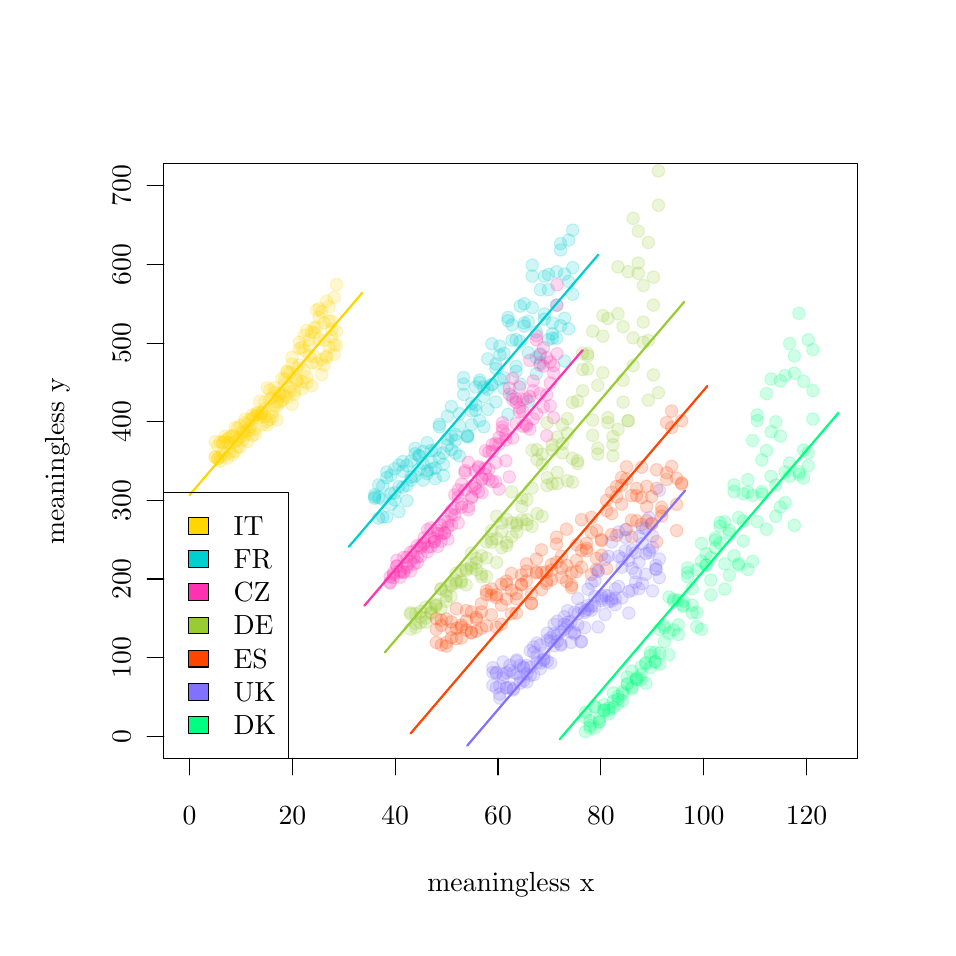
\begin{tikzpicture}[x=1pt,y=1pt]
\definecolor[named]{drawColor}{rgb}{0.00,0.00,0.00}
\definecolor[named]{fillColor}{rgb}{1.00,1.00,1.00}
\fill[color=fillColor,] (0,0) rectangle (325.21,325.21);
\begin{scope}
\path[clip] (  0.00,  0.00) rectangle (325.21,325.21);
\definecolor[named]{drawColor}{rgb}{0.24,0.00,0.33}
\definecolor[named]{drawColor}{rgb}{0.00,0.00,0.00}

\draw[color=drawColor,line cap=round,line join=round,fill opacity=0.00,] ( 58.49, 61.20) -- (281.44, 61.20);

\draw[color=drawColor,line cap=round,line join=round,fill opacity=0.00,] ( 58.49, 61.20) -- ( 58.49, 55.20);

\draw[color=drawColor,line cap=round,line join=round,fill opacity=0.00,] ( 95.65, 61.20) -- ( 95.65, 55.20);

\draw[color=drawColor,line cap=round,line join=round,fill opacity=0.00,] (132.80, 61.20) -- (132.80, 55.20);

\draw[color=drawColor,line cap=round,line join=round,fill opacity=0.00,] (169.96, 61.20) -- (169.96, 55.20);

\draw[color=drawColor,line cap=round,line join=round,fill opacity=0.00,] (207.12, 61.20) -- (207.12, 55.20);

\draw[color=drawColor,line cap=round,line join=round,fill opacity=0.00,] (244.28, 61.20) -- (244.28, 55.20);

\draw[color=drawColor,line cap=round,line join=round,fill opacity=0.00,] (281.44, 61.20) -- (281.44, 55.20);

\node[color=drawColor,anchor=base,inner sep=0pt, outer sep=0pt, scale=  1.00] at ( 58.49, 37.20) {0%
};

\node[color=drawColor,anchor=base,inner sep=0pt, outer sep=0pt, scale=  1.00] at ( 95.65, 37.20) {20%
};

\node[color=drawColor,anchor=base,inner sep=0pt, outer sep=0pt, scale=  1.00] at (132.80, 37.20) {40%
};

\node[color=drawColor,anchor=base,inner sep=0pt, outer sep=0pt, scale=  1.00] at (169.96, 37.20) {60%
};

\node[color=drawColor,anchor=base,inner sep=0pt, outer sep=0pt, scale=  1.00] at (207.12, 37.20) {80%
};

\node[color=drawColor,anchor=base,inner sep=0pt, outer sep=0pt, scale=  1.00] at (244.28, 37.20) {100%
};

\node[color=drawColor,anchor=base,inner sep=0pt, outer sep=0pt, scale=  1.00] at (281.44, 37.20) {120%
};

\draw[color=drawColor,line cap=round,line join=round,fill opacity=0.00,] ( 49.20, 69.16) -- ( 49.20,268.06);

\draw[color=drawColor,line cap=round,line join=round,fill opacity=0.00,] ( 49.20, 69.16) -- ( 43.20, 69.16);

\draw[color=drawColor,line cap=round,line join=round,fill opacity=0.00,] ( 49.20, 97.57) -- ( 43.20, 97.57);

\draw[color=drawColor,line cap=round,line join=round,fill opacity=0.00,] ( 49.20,125.99) -- ( 43.20,125.99);

\draw[color=drawColor,line cap=round,line join=round,fill opacity=0.00,] ( 49.20,154.40) -- ( 43.20,154.40);

\draw[color=drawColor,line cap=round,line join=round,fill opacity=0.00,] ( 49.20,182.81) -- ( 43.20,182.81);

\draw[color=drawColor,line cap=round,line join=round,fill opacity=0.00,] ( 49.20,211.23) -- ( 43.20,211.23);

\draw[color=drawColor,line cap=round,line join=round,fill opacity=0.00,] ( 49.20,239.64) -- ( 43.20,239.64);

\draw[color=drawColor,line cap=round,line join=round,fill opacity=0.00,] ( 49.20,268.06) -- ( 43.20,268.06);

\node[rotate= 90.00,color=drawColor,anchor=base,inner sep=0pt, outer sep=0pt, scale=  1.00] at ( 37.20, 69.16) {0%
};

\node[rotate= 90.00,color=drawColor,anchor=base,inner sep=0pt, outer sep=0pt, scale=  1.00] at ( 37.20, 97.57) {100%
};

\node[rotate= 90.00,color=drawColor,anchor=base,inner sep=0pt, outer sep=0pt, scale=  1.00] at ( 37.20,125.99) {200%
};

\node[rotate= 90.00,color=drawColor,anchor=base,inner sep=0pt, outer sep=0pt, scale=  1.00] at ( 37.20,154.40) {300%
};

\node[rotate= 90.00,color=drawColor,anchor=base,inner sep=0pt, outer sep=0pt, scale=  1.00] at ( 37.20,182.81) {400%
};

\node[rotate= 90.00,color=drawColor,anchor=base,inner sep=0pt, outer sep=0pt, scale=  1.00] at ( 37.20,211.23) {500%
};

\node[rotate= 90.00,color=drawColor,anchor=base,inner sep=0pt, outer sep=0pt, scale=  1.00] at ( 37.20,239.64) {600%
};

\node[rotate= 90.00,color=drawColor,anchor=base,inner sep=0pt, outer sep=0pt, scale=  1.00] at ( 37.20,268.06) {700%
};

\draw[color=drawColor,line cap=round,line join=round,fill opacity=0.00,] ( 49.20, 61.20) --
	(300.01, 61.20) --
	(300.01,276.01) --
	( 49.20,276.01) --
	( 49.20, 61.20);
\end{scope}
\begin{scope}
\path[clip] (  0.00,  0.00) rectangle (325.21,325.21);
\definecolor[named]{drawColor}{rgb}{0.24,0.00,0.33}
\definecolor[named]{drawColor}{rgb}{0.00,0.00,0.00}

\node[color=drawColor,anchor=base,inner sep=0pt, outer sep=0pt, scale=  1.00] at (174.61, 13.20) {meaningless x%
};

\node[rotate= 90.00,color=drawColor,anchor=base,inner sep=0pt, outer sep=0pt, scale=  1.00] at ( 13.20,168.61) {meaningless y%
};
\end{scope}
\begin{scope}
\path[clip] ( 49.20, 61.20) rectangle (300.01,276.01);
\definecolor[named]{drawColor}{rgb}{0.24,0.00,0.33}
\definecolor[named]{drawColor}{rgb}{1.00,0.84,0.00}
\definecolor[named]{fillColor}{rgb}{1.00,0.84,0.00}

\draw[color=drawColor,line cap=round,line join=round,fill=fillColor,fill opacity=0.19,draw opacity=0.19,] ( 67.78,170.07) circle (  2.25);

\draw[color=drawColor,line cap=round,line join=round,fill=fillColor,fill opacity=0.19,draw opacity=0.19,] ( 68.67,169.52) circle (  2.25);

\draw[color=drawColor,line cap=round,line join=round,fill=fillColor,fill opacity=0.19,draw opacity=0.19,] ( 69.57,170.04) circle (  2.25);

\draw[color=drawColor,line cap=round,line join=round,fill=fillColor,fill opacity=0.19,draw opacity=0.19,] ( 70.46,171.54) circle (  2.25);

\draw[color=drawColor,line cap=round,line join=round,fill=fillColor,fill opacity=0.19,draw opacity=0.19,] ( 71.36,175.95) circle (  2.25);

\draw[color=drawColor,line cap=round,line join=round,fill=fillColor,fill opacity=0.19,draw opacity=0.19,] ( 72.25,176.72) circle (  2.25);

\draw[color=drawColor,line cap=round,line join=round,fill=fillColor,fill opacity=0.19,draw opacity=0.19,] ( 73.14,171.70) circle (  2.25);

\draw[color=drawColor,line cap=round,line join=round,fill=fillColor,fill opacity=0.19,draw opacity=0.19,] ( 74.04,177.81) circle (  2.25);

\draw[color=drawColor,line cap=round,line join=round,fill=fillColor,fill opacity=0.19,draw opacity=0.19,] ( 74.93,180.69) circle (  2.25);

\draw[color=drawColor,line cap=round,line join=round,fill=fillColor,fill opacity=0.19,draw opacity=0.19,] ( 75.83,176.29) circle (  2.25);

\draw[color=drawColor,line cap=round,line join=round,fill=fillColor,fill opacity=0.19,draw opacity=0.19,] ( 76.72,181.26) circle (  2.25);

\draw[color=drawColor,line cap=round,line join=round,fill=fillColor,fill opacity=0.19,draw opacity=0.19,] ( 77.62,178.55) circle (  2.25);

\draw[color=drawColor,line cap=round,line join=round,fill=fillColor,fill opacity=0.19,draw opacity=0.19,] ( 78.51,182.45) circle (  2.25);

\draw[color=drawColor,line cap=round,line join=round,fill=fillColor,fill opacity=0.19,draw opacity=0.19,] ( 79.40,181.91) circle (  2.25);

\draw[color=drawColor,line cap=round,line join=round,fill=fillColor,fill opacity=0.19,draw opacity=0.19,] ( 80.30,179.85) circle (  2.25);

\draw[color=drawColor,line cap=round,line join=round,fill=fillColor,fill opacity=0.19,draw opacity=0.19,] ( 81.19,185.24) circle (  2.25);

\draw[color=drawColor,line cap=round,line join=round,fill=fillColor,fill opacity=0.19,draw opacity=0.19,] ( 82.09,184.92) circle (  2.25);

\draw[color=drawColor,line cap=round,line join=round,fill=fillColor,fill opacity=0.19,draw opacity=0.19,] ( 82.98,185.23) circle (  2.25);

\draw[color=drawColor,line cap=round,line join=round,fill=fillColor,fill opacity=0.19,draw opacity=0.19,] ( 83.87,185.23) circle (  2.25);

\draw[color=drawColor,line cap=round,line join=round,fill=fillColor,fill opacity=0.19,draw opacity=0.19,] ( 84.77,186.27) circle (  2.25);

\draw[color=drawColor,line cap=round,line join=round,fill=fillColor,fill opacity=0.19,draw opacity=0.19,] ( 85.66,189.92) circle (  2.25);

\draw[color=drawColor,line cap=round,line join=round,fill=fillColor,fill opacity=0.19,draw opacity=0.19,] ( 86.56,195.08) circle (  2.25);

\draw[color=drawColor,line cap=round,line join=round,fill=fillColor,fill opacity=0.19,draw opacity=0.19,] ( 87.45,183.59) circle (  2.25);

\draw[color=drawColor,line cap=round,line join=round,fill=fillColor,fill opacity=0.19,draw opacity=0.19,] ( 88.35,191.36) circle (  2.25);

\draw[color=drawColor,line cap=round,line join=round,fill=fillColor,fill opacity=0.19,draw opacity=0.19,] ( 89.24,195.07) circle (  2.25);

\draw[color=drawColor,line cap=round,line join=round,fill=fillColor,fill opacity=0.19,draw opacity=0.19,] ( 90.13,188.45) circle (  2.25);

\draw[color=drawColor,line cap=round,line join=round,fill=fillColor,fill opacity=0.19,draw opacity=0.19,] ( 91.03,193.10) circle (  2.25);

\draw[color=drawColor,line cap=round,line join=round,fill=fillColor,fill opacity=0.19,draw opacity=0.19,] ( 91.92,198.51) circle (  2.25);

\draw[color=drawColor,line cap=round,line join=round,fill=fillColor,fill opacity=0.19,draw opacity=0.19,] ( 92.82,196.27) circle (  2.25);

\draw[color=drawColor,line cap=round,line join=round,fill=fillColor,fill opacity=0.19,draw opacity=0.19,] ( 93.71,191.59) circle (  2.25);

\draw[color=drawColor,line cap=round,line join=round,fill=fillColor,fill opacity=0.19,draw opacity=0.19,] ( 94.61,193.56) circle (  2.25);

\draw[color=drawColor,line cap=round,line join=round,fill=fillColor,fill opacity=0.19,draw opacity=0.19,] ( 95.50,206.14) circle (  2.25);

\draw[color=drawColor,line cap=round,line join=round,fill=fillColor,fill opacity=0.19,draw opacity=0.19,] ( 96.39,192.68) circle (  2.25);

\draw[color=drawColor,line cap=round,line join=round,fill=fillColor,fill opacity=0.19,draw opacity=0.19,] ( 97.29,197.94) circle (  2.25);

\draw[color=drawColor,line cap=round,line join=round,fill=fillColor,fill opacity=0.19,draw opacity=0.19,] ( 98.18,209.29) circle (  2.25);

\draw[color=drawColor,line cap=round,line join=round,fill=fillColor,fill opacity=0.19,draw opacity=0.19,] ( 99.08,194.66) circle (  2.25);

\draw[color=drawColor,line cap=round,line join=round,fill=fillColor,fill opacity=0.19,draw opacity=0.19,] ( 99.97,208.52) circle (  2.25);

\draw[color=drawColor,line cap=round,line join=round,fill=fillColor,fill opacity=0.19,draw opacity=0.19,] (100.86,198.95) circle (  2.25);

\draw[color=drawColor,line cap=round,line join=round,fill=fillColor,fill opacity=0.19,draw opacity=0.19,] (101.76,206.67) circle (  2.25);

\draw[color=drawColor,line cap=round,line join=round,fill=fillColor,fill opacity=0.19,draw opacity=0.19,] (102.65,195.77) circle (  2.25);

\draw[color=drawColor,line cap=round,line join=round,fill=fillColor,fill opacity=0.19,draw opacity=0.19,] (103.55,216.74) circle (  2.25);

\draw[color=drawColor,line cap=round,line join=round,fill=fillColor,fill opacity=0.19,draw opacity=0.19,] (104.44,223.15) circle (  2.25);

\draw[color=drawColor,line cap=round,line join=round,fill=fillColor,fill opacity=0.19,draw opacity=0.19,] (105.34,220.64) circle (  2.25);

\draw[color=drawColor,line cap=round,line join=round,fill=fillColor,fill opacity=0.19,draw opacity=0.19,] (106.23,205.27) circle (  2.25);

\draw[color=drawColor,line cap=round,line join=round,fill=fillColor,fill opacity=0.19,draw opacity=0.19,] (107.12,218.51) circle (  2.25);

\draw[color=drawColor,line cap=round,line join=round,fill=fillColor,fill opacity=0.19,draw opacity=0.19,] (108.02,206.09) circle (  2.25);

\draw[color=drawColor,line cap=round,line join=round,fill=fillColor,fill opacity=0.19,draw opacity=0.19,] (108.91,219.19) circle (  2.25);

\draw[color=drawColor,line cap=round,line join=round,fill=fillColor,fill opacity=0.19,draw opacity=0.19,] (109.81,213.53) circle (  2.25);

\draw[color=drawColor,line cap=round,line join=round,fill=fillColor,fill opacity=0.19,draw opacity=0.19,] (110.70,207.11) circle (  2.25);

\draw[color=drawColor,line cap=round,line join=round,fill=fillColor,fill opacity=0.19,draw opacity=0.19,] (111.60,210.53) circle (  2.25);

\draw[color=drawColor,line cap=round,line join=round,fill=fillColor,fill opacity=0.19,draw opacity=0.19,] ( 67.78,175.54) circle (  2.25);

\draw[color=drawColor,line cap=round,line join=round,fill=fillColor,fill opacity=0.19,draw opacity=0.19,] ( 68.67,174.10) circle (  2.25);

\draw[color=drawColor,line cap=round,line join=round,fill=fillColor,fill opacity=0.19,draw opacity=0.19,] ( 69.57,168.60) circle (  2.25);

\draw[color=drawColor,line cap=round,line join=round,fill=fillColor,fill opacity=0.19,draw opacity=0.19,] ( 70.46,175.23) circle (  2.25);

\draw[color=drawColor,line cap=round,line join=round,fill=fillColor,fill opacity=0.19,draw opacity=0.19,] ( 71.36,177.57) circle (  2.25);

\draw[color=drawColor,line cap=round,line join=round,fill=fillColor,fill opacity=0.19,draw opacity=0.19,] ( 72.25,175.36) circle (  2.25);

\draw[color=drawColor,line cap=round,line join=round,fill=fillColor,fill opacity=0.19,draw opacity=0.19,] ( 73.14,175.00) circle (  2.25);

\draw[color=drawColor,line cap=round,line join=round,fill=fillColor,fill opacity=0.19,draw opacity=0.19,] ( 74.04,177.58) circle (  2.25);

\draw[color=drawColor,line cap=round,line join=round,fill=fillColor,fill opacity=0.19,draw opacity=0.19,] ( 74.93,172.14) circle (  2.25);

\draw[color=drawColor,line cap=round,line join=round,fill=fillColor,fill opacity=0.19,draw opacity=0.19,] ( 75.83,173.71) circle (  2.25);

\draw[color=drawColor,line cap=round,line join=round,fill=fillColor,fill opacity=0.19,draw opacity=0.19,] ( 76.72,173.63) circle (  2.25);

\draw[color=drawColor,line cap=round,line join=round,fill=fillColor,fill opacity=0.19,draw opacity=0.19,] ( 77.62,179.32) circle (  2.25);

\draw[color=drawColor,line cap=round,line join=round,fill=fillColor,fill opacity=0.19,draw opacity=0.19,] ( 78.51,177.97) circle (  2.25);

\draw[color=drawColor,line cap=round,line join=round,fill=fillColor,fill opacity=0.19,draw opacity=0.19,] ( 79.40,175.60) circle (  2.25);

\draw[color=drawColor,line cap=round,line join=round,fill=fillColor,fill opacity=0.19,draw opacity=0.19,] ( 80.30,183.55) circle (  2.25);

\draw[color=drawColor,line cap=round,line join=round,fill=fillColor,fill opacity=0.19,draw opacity=0.19,] ( 81.19,177.85) circle (  2.25);

\draw[color=drawColor,line cap=round,line join=round,fill=fillColor,fill opacity=0.19,draw opacity=0.19,] ( 82.09,180.07) circle (  2.25);

\draw[color=drawColor,line cap=round,line join=round,fill=fillColor,fill opacity=0.19,draw opacity=0.19,] ( 82.98,186.14) circle (  2.25);

\draw[color=drawColor,line cap=round,line join=round,fill=fillColor,fill opacity=0.19,draw opacity=0.19,] ( 83.87,190.21) circle (  2.25);

\draw[color=drawColor,line cap=round,line join=round,fill=fillColor,fill opacity=0.19,draw opacity=0.19,] ( 84.77,185.80) circle (  2.25);

\draw[color=drawColor,line cap=round,line join=round,fill=fillColor,fill opacity=0.19,draw opacity=0.19,] ( 85.66,184.69) circle (  2.25);

\draw[color=drawColor,line cap=round,line join=round,fill=fillColor,fill opacity=0.19,draw opacity=0.19,] ( 86.56,181.69) circle (  2.25);

\draw[color=drawColor,line cap=round,line join=round,fill=fillColor,fill opacity=0.19,draw opacity=0.19,] ( 87.45,194.35) circle (  2.25);

\draw[color=drawColor,line cap=round,line join=round,fill=fillColor,fill opacity=0.19,draw opacity=0.19,] ( 88.35,184.59) circle (  2.25);

\draw[color=drawColor,line cap=round,line join=round,fill=fillColor,fill opacity=0.19,draw opacity=0.19,] ( 89.24,188.65) circle (  2.25);

\draw[color=drawColor,line cap=round,line join=round,fill=fillColor,fill opacity=0.19,draw opacity=0.19,] ( 90.13,183.54) circle (  2.25);

\draw[color=drawColor,line cap=round,line join=round,fill=fillColor,fill opacity=0.19,draw opacity=0.19,] ( 91.03,189.81) circle (  2.25);

\draw[color=drawColor,line cap=round,line join=round,fill=fillColor,fill opacity=0.19,draw opacity=0.19,] ( 91.92,193.02) circle (  2.25);

\draw[color=drawColor,line cap=round,line join=round,fill=fillColor,fill opacity=0.19,draw opacity=0.19,] ( 92.82,198.23) circle (  2.25);

\draw[color=drawColor,line cap=round,line join=round,fill=fillColor,fill opacity=0.19,draw opacity=0.19,] ( 93.71,201.16) circle (  2.25);

\draw[color=drawColor,line cap=round,line join=round,fill=fillColor,fill opacity=0.19,draw opacity=0.19,] ( 94.61,200.42) circle (  2.25);

\draw[color=drawColor,line cap=round,line join=round,fill=fillColor,fill opacity=0.19,draw opacity=0.19,] ( 95.50,189.06) circle (  2.25);

\draw[color=drawColor,line cap=round,line join=round,fill=fillColor,fill opacity=0.19,draw opacity=0.19,] ( 96.39,193.97) circle (  2.25);

\draw[color=drawColor,line cap=round,line join=round,fill=fillColor,fill opacity=0.19,draw opacity=0.19,] ( 97.29,197.34) circle (  2.25);

\draw[color=drawColor,line cap=round,line join=round,fill=fillColor,fill opacity=0.19,draw opacity=0.19,] ( 98.18,211.56) circle (  2.25);

\draw[color=drawColor,line cap=round,line join=round,fill=fillColor,fill opacity=0.19,draw opacity=0.19,] ( 99.08,197.24) circle (  2.25);

\draw[color=drawColor,line cap=round,line join=round,fill=fillColor,fill opacity=0.19,draw opacity=0.19,] ( 99.97,214.05) circle (  2.25);

\draw[color=drawColor,line cap=round,line join=round,fill=fillColor,fill opacity=0.19,draw opacity=0.19,] (100.86,215.81) circle (  2.25);

\draw[color=drawColor,line cap=round,line join=round,fill=fillColor,fill opacity=0.19,draw opacity=0.19,] (101.76,212.45) circle (  2.25);

\draw[color=drawColor,line cap=round,line join=round,fill=fillColor,fill opacity=0.19,draw opacity=0.19,] (102.65,215.21) circle (  2.25);

\draw[color=drawColor,line cap=round,line join=round,fill=fillColor,fill opacity=0.19,draw opacity=0.19,] (103.55,206.27) circle (  2.25);

\draw[color=drawColor,line cap=round,line join=round,fill=fillColor,fill opacity=0.19,draw opacity=0.19,] (104.44,203.85) circle (  2.25);

\draw[color=drawColor,line cap=round,line join=round,fill=fillColor,fill opacity=0.19,draw opacity=0.19,] (105.34,212.64) circle (  2.25);

\draw[color=drawColor,line cap=round,line join=round,fill=fillColor,fill opacity=0.19,draw opacity=0.19,] (106.23,199.82) circle (  2.25);

\draw[color=drawColor,line cap=round,line join=round,fill=fillColor,fill opacity=0.19,draw opacity=0.19,] (107.12,212.15) circle (  2.25);

\draw[color=drawColor,line cap=round,line join=round,fill=fillColor,fill opacity=0.19,draw opacity=0.19,] (108.02,226.32) circle (  2.25);

\draw[color=drawColor,line cap=round,line join=round,fill=fillColor,fill opacity=0.19,draw opacity=0.19,] (108.91,224.45) circle (  2.25);

\draw[color=drawColor,line cap=round,line join=round,fill=fillColor,fill opacity=0.19,draw opacity=0.19,] (109.81,216.16) circle (  2.25);

\draw[color=drawColor,line cap=round,line join=round,fill=fillColor,fill opacity=0.19,draw opacity=0.19,] (110.70,227.70) circle (  2.25);

\draw[color=drawColor,line cap=round,line join=round,fill=fillColor,fill opacity=0.19,draw opacity=0.19,] (111.60,215.41) circle (  2.25);

\draw[color=drawColor,line cap=round,line join=round,fill=fillColor,fill opacity=0.19,draw opacity=0.19,] ( 67.78,170.07) circle (  2.25);

\draw[color=drawColor,line cap=round,line join=round,fill=fillColor,fill opacity=0.19,draw opacity=0.19,] ( 68.67,169.40) circle (  2.25);

\draw[color=drawColor,line cap=round,line join=round,fill=fillColor,fill opacity=0.19,draw opacity=0.19,] ( 69.57,175.55) circle (  2.25);

\draw[color=drawColor,line cap=round,line join=round,fill=fillColor,fill opacity=0.19,draw opacity=0.19,] ( 70.46,175.35) circle (  2.25);

\draw[color=drawColor,line cap=round,line join=round,fill=fillColor,fill opacity=0.19,draw opacity=0.19,] ( 71.36,171.02) circle (  2.25);

\draw[color=drawColor,line cap=round,line join=round,fill=fillColor,fill opacity=0.19,draw opacity=0.19,] ( 72.25,169.64) circle (  2.25);

\draw[color=drawColor,line cap=round,line join=round,fill=fillColor,fill opacity=0.19,draw opacity=0.19,] ( 73.14,177.35) circle (  2.25);

\draw[color=drawColor,line cap=round,line join=round,fill=fillColor,fill opacity=0.19,draw opacity=0.19,] ( 74.04,170.91) circle (  2.25);

\draw[color=drawColor,line cap=round,line join=round,fill=fillColor,fill opacity=0.19,draw opacity=0.19,] ( 74.93,175.63) circle (  2.25);

\draw[color=drawColor,line cap=round,line join=round,fill=fillColor,fill opacity=0.19,draw opacity=0.19,] ( 75.83,180.48) circle (  2.25);

\draw[color=drawColor,line cap=round,line join=round,fill=fillColor,fill opacity=0.19,draw opacity=0.19,] ( 76.72,177.29) circle (  2.25);

\draw[color=drawColor,line cap=round,line join=round,fill=fillColor,fill opacity=0.19,draw opacity=0.19,] ( 77.62,176.08) circle (  2.25);

\draw[color=drawColor,line cap=round,line join=round,fill=fillColor,fill opacity=0.19,draw opacity=0.19,] ( 78.51,183.73) circle (  2.25);

\draw[color=drawColor,line cap=round,line join=round,fill=fillColor,fill opacity=0.19,draw opacity=0.19,] ( 79.40,179.65) circle (  2.25);

\draw[color=drawColor,line cap=round,line join=round,fill=fillColor,fill opacity=0.19,draw opacity=0.19,] ( 80.30,180.93) circle (  2.25);

\draw[color=drawColor,line cap=round,line join=round,fill=fillColor,fill opacity=0.19,draw opacity=0.19,] ( 81.19,183.94) circle (  2.25);

\draw[color=drawColor,line cap=round,line join=round,fill=fillColor,fill opacity=0.19,draw opacity=0.19,] ( 82.09,178.21) circle (  2.25);

\draw[color=drawColor,line cap=round,line join=round,fill=fillColor,fill opacity=0.19,draw opacity=0.19,] ( 82.98,185.91) circle (  2.25);

\draw[color=drawColor,line cap=round,line join=round,fill=fillColor,fill opacity=0.19,draw opacity=0.19,] ( 83.87,184.35) circle (  2.25);

\draw[color=drawColor,line cap=round,line join=round,fill=fillColor,fill opacity=0.19,draw opacity=0.19,] ( 84.77,181.69) circle (  2.25);

\draw[color=drawColor,line cap=round,line join=round,fill=fillColor,fill opacity=0.19,draw opacity=0.19,] ( 85.66,187.52) circle (  2.25);

\draw[color=drawColor,line cap=round,line join=round,fill=fillColor,fill opacity=0.19,draw opacity=0.19,] ( 86.56,182.93) circle (  2.25);

\draw[color=drawColor,line cap=round,line join=round,fill=fillColor,fill opacity=0.19,draw opacity=0.19,] ( 87.45,190.97) circle (  2.25);

\draw[color=drawColor,line cap=round,line join=round,fill=fillColor,fill opacity=0.19,draw opacity=0.19,] ( 88.35,186.04) circle (  2.25);

\draw[color=drawColor,line cap=round,line join=round,fill=fillColor,fill opacity=0.19,draw opacity=0.19,] ( 89.24,193.40) circle (  2.25);

\draw[color=drawColor,line cap=round,line join=round,fill=fillColor,fill opacity=0.19,draw opacity=0.19,] ( 90.13,190.07) circle (  2.25);

\draw[color=drawColor,line cap=round,line join=round,fill=fillColor,fill opacity=0.19,draw opacity=0.19,] ( 91.03,192.01) circle (  2.25);

\draw[color=drawColor,line cap=round,line join=round,fill=fillColor,fill opacity=0.19,draw opacity=0.19,] ( 91.92,190.34) circle (  2.25);

\draw[color=drawColor,line cap=round,line join=round,fill=fillColor,fill opacity=0.19,draw opacity=0.19,] ( 92.82,192.18) circle (  2.25);

\draw[color=drawColor,line cap=round,line join=round,fill=fillColor,fill opacity=0.19,draw opacity=0.19,] ( 93.71,200.78) circle (  2.25);

\draw[color=drawColor,line cap=round,line join=round,fill=fillColor,fill opacity=0.19,draw opacity=0.19,] ( 94.61,195.23) circle (  2.25);

\draw[color=drawColor,line cap=round,line join=round,fill=fillColor,fill opacity=0.19,draw opacity=0.19,] ( 95.50,203.62) circle (  2.25);

\draw[color=drawColor,line cap=round,line join=round,fill=fillColor,fill opacity=0.19,draw opacity=0.19,] ( 96.39,198.81) circle (  2.25);

\draw[color=drawColor,line cap=round,line join=round,fill=fillColor,fill opacity=0.19,draw opacity=0.19,] ( 97.29,202.13) circle (  2.25);

\draw[color=drawColor,line cap=round,line join=round,fill=fillColor,fill opacity=0.19,draw opacity=0.19,] ( 98.18,203.30) circle (  2.25);

\draw[color=drawColor,line cap=round,line join=round,fill=fillColor,fill opacity=0.19,draw opacity=0.19,] ( 99.08,209.61) circle (  2.25);

\draw[color=drawColor,line cap=round,line join=round,fill=fillColor,fill opacity=0.19,draw opacity=0.19,] ( 99.97,201.46) circle (  2.25);

\draw[color=drawColor,line cap=round,line join=round,fill=fillColor,fill opacity=0.19,draw opacity=0.19,] (100.86,196.83) circle (  2.25);

\draw[color=drawColor,line cap=round,line join=round,fill=fillColor,fill opacity=0.19,draw opacity=0.19,] (101.76,210.24) circle (  2.25);

\draw[color=drawColor,line cap=round,line join=round,fill=fillColor,fill opacity=0.19,draw opacity=0.19,] (102.65,204.15) circle (  2.25);

\draw[color=drawColor,line cap=round,line join=round,fill=fillColor,fill opacity=0.19,draw opacity=0.19,] (103.55,215.00) circle (  2.25);

\draw[color=drawColor,line cap=round,line join=round,fill=fillColor,fill opacity=0.19,draw opacity=0.19,] (104.44,217.01) circle (  2.25);

\draw[color=drawColor,line cap=round,line join=round,fill=fillColor,fill opacity=0.19,draw opacity=0.19,] (105.34,223.69) circle (  2.25);

\draw[color=drawColor,line cap=round,line join=round,fill=fillColor,fill opacity=0.19,draw opacity=0.19,] (106.23,222.64) circle (  2.25);

\draw[color=drawColor,line cap=round,line join=round,fill=fillColor,fill opacity=0.19,draw opacity=0.19,] (107.12,203.27) circle (  2.25);

\draw[color=drawColor,line cap=round,line join=round,fill=fillColor,fill opacity=0.19,draw opacity=0.19,] (108.02,206.61) circle (  2.25);

\draw[color=drawColor,line cap=round,line join=round,fill=fillColor,fill opacity=0.19,draw opacity=0.19,] (108.91,209.73) circle (  2.25);

\draw[color=drawColor,line cap=round,line join=round,fill=fillColor,fill opacity=0.19,draw opacity=0.19,] (109.81,219.21) circle (  2.25);

\draw[color=drawColor,line cap=round,line join=round,fill=fillColor,fill opacity=0.19,draw opacity=0.19,] (110.70,210.70) circle (  2.25);

\draw[color=drawColor,line cap=round,line join=round,fill=fillColor,fill opacity=0.19,draw opacity=0.19,] (111.60,232.38) circle (  2.25);
\definecolor[named]{drawColor}{rgb}{0.00,0.81,0.82}
\definecolor[named]{fillColor}{rgb}{0.00,0.81,0.82}

\draw[color=drawColor,line cap=round,line join=round,fill=fillColor,fill opacity=0.19,draw opacity=0.19,] (125.37,155.16) circle (  2.25);

\draw[color=drawColor,line cap=round,line join=round,fill=fillColor,fill opacity=0.19,draw opacity=0.19,] (126.83,159.99) circle (  2.25);

\draw[color=drawColor,line cap=round,line join=round,fill=fillColor,fill opacity=0.19,draw opacity=0.19,] (128.29,159.59) circle (  2.25);

\draw[color=drawColor,line cap=round,line join=round,fill=fillColor,fill opacity=0.19,draw opacity=0.19,] (129.75,148.39) circle (  2.25);

\draw[color=drawColor,line cap=round,line join=round,fill=fillColor,fill opacity=0.19,draw opacity=0.19,] (131.21,163.44) circle (  2.25);

\draw[color=drawColor,line cap=round,line join=round,fill=fillColor,fill opacity=0.19,draw opacity=0.19,] (132.68,154.58) circle (  2.25);

\draw[color=drawColor,line cap=round,line join=round,fill=fillColor,fill opacity=0.19,draw opacity=0.19,] (134.14,150.31) circle (  2.25);

\draw[color=drawColor,line cap=round,line join=round,fill=fillColor,fill opacity=0.19,draw opacity=0.19,] (135.60,164.93) circle (  2.25);

\draw[color=drawColor,line cap=round,line join=round,fill=fillColor,fill opacity=0.19,draw opacity=0.19,] (137.06,154.27) circle (  2.25);

\draw[color=drawColor,line cap=round,line join=round,fill=fillColor,fill opacity=0.19,draw opacity=0.19,] (138.52,162.86) circle (  2.25);

\draw[color=drawColor,line cap=round,line join=round,fill=fillColor,fill opacity=0.19,draw opacity=0.19,] (139.98,171.25) circle (  2.25);

\draw[color=drawColor,line cap=round,line join=round,fill=fillColor,fill opacity=0.19,draw opacity=0.19,] (141.44,170.30) circle (  2.25);

\draw[color=drawColor,line cap=round,line join=round,fill=fillColor,fill opacity=0.19,draw opacity=0.19,] (142.90,167.74) circle (  2.25);

\draw[color=drawColor,line cap=round,line join=round,fill=fillColor,fill opacity=0.19,draw opacity=0.19,] (144.36,175.26) circle (  2.25);

\draw[color=drawColor,line cap=round,line join=round,fill=fillColor,fill opacity=0.19,draw opacity=0.19,] (145.82,165.65) circle (  2.25);

\draw[color=drawColor,line cap=round,line join=round,fill=fillColor,fill opacity=0.19,draw opacity=0.19,] (147.28,162.24) circle (  2.25);

\draw[color=drawColor,line cap=round,line join=round,fill=fillColor,fill opacity=0.19,draw opacity=0.19,] (148.74,180.98) circle (  2.25);

\draw[color=drawColor,line cap=round,line join=round,fill=fillColor,fill opacity=0.19,draw opacity=0.19,] (150.20,163.42) circle (  2.25);

\draw[color=drawColor,line cap=round,line join=round,fill=fillColor,fill opacity=0.19,draw opacity=0.19,] (151.66,176.50) circle (  2.25);

\draw[color=drawColor,line cap=round,line join=round,fill=fillColor,fill opacity=0.19,draw opacity=0.19,] (153.12,177.49) circle (  2.25);

\draw[color=drawColor,line cap=round,line join=round,fill=fillColor,fill opacity=0.19,draw opacity=0.19,] (154.58,176.08) circle (  2.25);

\draw[color=drawColor,line cap=round,line join=round,fill=fillColor,fill opacity=0.19,draw opacity=0.19,] (156.04,185.71) circle (  2.25);

\draw[color=drawColor,line cap=round,line join=round,fill=fillColor,fill opacity=0.19,draw opacity=0.19,] (157.50,196.39) circle (  2.25);

\draw[color=drawColor,line cap=round,line join=round,fill=fillColor,fill opacity=0.19,draw opacity=0.19,] (158.96,177.37) circle (  2.25);

\draw[color=drawColor,line cap=round,line join=round,fill=fillColor,fill opacity=0.19,draw opacity=0.19,] (160.42,181.74) circle (  2.25);

\draw[color=drawColor,line cap=round,line join=round,fill=fillColor,fill opacity=0.19,draw opacity=0.19,] (161.88,186.95) circle (  2.25);

\draw[color=drawColor,line cap=round,line join=round,fill=fillColor,fill opacity=0.19,draw opacity=0.19,] (163.34,183.23) circle (  2.25);

\draw[color=drawColor,line cap=round,line join=round,fill=fillColor,fill opacity=0.19,draw opacity=0.19,] (164.80,195.31) circle (  2.25);

\draw[color=drawColor,line cap=round,line join=round,fill=fillColor,fill opacity=0.19,draw opacity=0.19,] (166.26,187.28) circle (  2.25);

\draw[color=drawColor,line cap=round,line join=round,fill=fillColor,fill opacity=0.19,draw opacity=0.19,] (167.72,210.98) circle (  2.25);

\draw[color=drawColor,line cap=round,line join=round,fill=fillColor,fill opacity=0.19,draw opacity=0.19,] (169.18,189.96) circle (  2.25);

\draw[color=drawColor,line cap=round,line join=round,fill=fillColor,fill opacity=0.19,draw opacity=0.19,] (170.64,206.93) circle (  2.25);

\draw[color=drawColor,line cap=round,line join=round,fill=fillColor,fill opacity=0.19,draw opacity=0.19,] (172.10,207.52) circle (  2.25);

\draw[color=drawColor,line cap=round,line join=round,fill=fillColor,fill opacity=0.19,draw opacity=0.19,] (173.56,220.51) circle (  2.25);

\draw[color=drawColor,line cap=round,line join=round,fill=fillColor,fill opacity=0.19,draw opacity=0.19,] (175.02,191.97) circle (  2.25);

\draw[color=drawColor,line cap=round,line join=round,fill=fillColor,fill opacity=0.19,draw opacity=0.19,] (176.49,202.78) circle (  2.25);

\draw[color=drawColor,line cap=round,line join=round,fill=fillColor,fill opacity=0.19,draw opacity=0.19,] (177.95,211.80) circle (  2.25);

\draw[color=drawColor,line cap=round,line join=round,fill=fillColor,fill opacity=0.19,draw opacity=0.19,] (179.41,225.48) circle (  2.25);

\draw[color=drawColor,line cap=round,line join=round,fill=fillColor,fill opacity=0.19,draw opacity=0.19,] (180.87,207.75) circle (  2.25);

\draw[color=drawColor,line cap=round,line join=round,fill=fillColor,fill opacity=0.19,draw opacity=0.19,] (182.33,235.42) circle (  2.25);

\draw[color=drawColor,line cap=round,line join=round,fill=fillColor,fill opacity=0.19,draw opacity=0.19,] (183.79,206.00) circle (  2.25);

\draw[color=drawColor,line cap=round,line join=round,fill=fillColor,fill opacity=0.19,draw opacity=0.19,] (185.25,207.39) circle (  2.25);

\draw[color=drawColor,line cap=round,line join=round,fill=fillColor,fill opacity=0.19,draw opacity=0.19,] (186.71,219.88) circle (  2.25);

\draw[color=drawColor,line cap=round,line join=round,fill=fillColor,fill opacity=0.19,draw opacity=0.19,] (188.17,212.49) circle (  2.25);

\draw[color=drawColor,line cap=round,line join=round,fill=fillColor,fill opacity=0.19,draw opacity=0.19,] (189.63,213.00) circle (  2.25);

\draw[color=drawColor,line cap=round,line join=round,fill=fillColor,fill opacity=0.19,draw opacity=0.19,] (191.09,225.01) circle (  2.25);

\draw[color=drawColor,line cap=round,line join=round,fill=fillColor,fill opacity=0.19,draw opacity=0.19,] (192.55,244.88) circle (  2.25);

\draw[color=drawColor,line cap=round,line join=round,fill=fillColor,fill opacity=0.19,draw opacity=0.19,] (194.01,220.23) circle (  2.25);

\draw[color=drawColor,line cap=round,line join=round,fill=fillColor,fill opacity=0.19,draw opacity=0.19,] (195.47,248.45) circle (  2.25);

\draw[color=drawColor,line cap=round,line join=round,fill=fillColor,fill opacity=0.19,draw opacity=0.19,] (196.93,228.87) circle (  2.25);

\draw[color=drawColor,line cap=round,line join=round,fill=fillColor,fill opacity=0.19,draw opacity=0.19,] (125.37,156.42) circle (  2.25);

\draw[color=drawColor,line cap=round,line join=round,fill=fillColor,fill opacity=0.19,draw opacity=0.19,] (126.83,147.95) circle (  2.25);

\draw[color=drawColor,line cap=round,line join=round,fill=fillColor,fill opacity=0.19,draw opacity=0.19,] (128.29,154.79) circle (  2.25);

\draw[color=drawColor,line cap=round,line join=round,fill=fillColor,fill opacity=0.19,draw opacity=0.19,] (129.75,162.62) circle (  2.25);

\draw[color=drawColor,line cap=round,line join=round,fill=fillColor,fill opacity=0.19,draw opacity=0.19,] (131.21,152.97) circle (  2.25);

\draw[color=drawColor,line cap=round,line join=round,fill=fillColor,fill opacity=0.19,draw opacity=0.19,] (132.68,165.83) circle (  2.25);

\draw[color=drawColor,line cap=round,line join=round,fill=fillColor,fill opacity=0.19,draw opacity=0.19,] (134.14,159.38) circle (  2.25);

\draw[color=drawColor,line cap=round,line join=round,fill=fillColor,fill opacity=0.19,draw opacity=0.19,] (135.60,168.44) circle (  2.25);

\draw[color=drawColor,line cap=round,line join=round,fill=fillColor,fill opacity=0.19,draw opacity=0.19,] (137.06,159.79) circle (  2.25);

\draw[color=drawColor,line cap=round,line join=round,fill=fillColor,fill opacity=0.19,draw opacity=0.19,] (138.52,168.67) circle (  2.25);

\draw[color=drawColor,line cap=round,line join=round,fill=fillColor,fill opacity=0.19,draw opacity=0.19,] (139.98,163.14) circle (  2.25);

\draw[color=drawColor,line cap=round,line join=round,fill=fillColor,fill opacity=0.19,draw opacity=0.19,] (141.44,170.67) circle (  2.25);

\draw[color=drawColor,line cap=round,line join=round,fill=fillColor,fill opacity=0.19,draw opacity=0.19,] (142.90,172.07) circle (  2.25);

\draw[color=drawColor,line cap=round,line join=round,fill=fillColor,fill opacity=0.19,draw opacity=0.19,] (144.36,164.09) circle (  2.25);

\draw[color=drawColor,line cap=round,line join=round,fill=fillColor,fill opacity=0.19,draw opacity=0.19,] (145.82,172.40) circle (  2.25);

\draw[color=drawColor,line cap=round,line join=round,fill=fillColor,fill opacity=0.19,draw opacity=0.19,] (147.28,166.10) circle (  2.25);

\draw[color=drawColor,line cap=round,line join=round,fill=fillColor,fill opacity=0.19,draw opacity=0.19,] (148.74,181.90) circle (  2.25);

\draw[color=drawColor,line cap=round,line join=round,fill=fillColor,fill opacity=0.19,draw opacity=0.19,] (150.20,167.38) circle (  2.25);

\draw[color=drawColor,line cap=round,line join=round,fill=fillColor,fill opacity=0.19,draw opacity=0.19,] (151.66,174.23) circle (  2.25);

\draw[color=drawColor,line cap=round,line join=round,fill=fillColor,fill opacity=0.19,draw opacity=0.19,] (153.12,188.30) circle (  2.25);

\draw[color=drawColor,line cap=round,line join=round,fill=fillColor,fill opacity=0.19,draw opacity=0.19,] (154.58,178.19) circle (  2.25);

\draw[color=drawColor,line cap=round,line join=round,fill=fillColor,fill opacity=0.19,draw opacity=0.19,] (156.04,181.30) circle (  2.25);

\draw[color=drawColor,line cap=round,line join=round,fill=fillColor,fill opacity=0.19,draw opacity=0.19,] (157.50,192.69) circle (  2.25);

\draw[color=drawColor,line cap=round,line join=round,fill=fillColor,fill opacity=0.19,draw opacity=0.19,] (158.96,177.85) circle (  2.25);

\draw[color=drawColor,line cap=round,line join=round,fill=fillColor,fill opacity=0.19,draw opacity=0.19,] (160.42,189.46) circle (  2.25);

\draw[color=drawColor,line cap=round,line join=round,fill=fillColor,fill opacity=0.19,draw opacity=0.19,] (161.88,188.89) circle (  2.25);

\draw[color=drawColor,line cap=round,line join=round,fill=fillColor,fill opacity=0.19,draw opacity=0.19,] (163.34,197.02) circle (  2.25);

\draw[color=drawColor,line cap=round,line join=round,fill=fillColor,fill opacity=0.19,draw opacity=0.19,] (164.80,180.98) circle (  2.25);

\draw[color=drawColor,line cap=round,line join=round,fill=fillColor,fill opacity=0.19,draw opacity=0.19,] (166.26,205.56) circle (  2.25);

\draw[color=drawColor,line cap=round,line join=round,fill=fillColor,fill opacity=0.19,draw opacity=0.19,] (167.72,196.10) circle (  2.25);

\draw[color=drawColor,line cap=round,line join=round,fill=fillColor,fill opacity=0.19,draw opacity=0.19,] (169.18,203.69) circle (  2.25);

\draw[color=drawColor,line cap=round,line join=round,fill=fillColor,fill opacity=0.19,draw opacity=0.19,] (170.64,210.10) circle (  2.25);

\draw[color=drawColor,line cap=round,line join=round,fill=fillColor,fill opacity=0.19,draw opacity=0.19,] (172.10,194.83) circle (  2.25);

\draw[color=drawColor,line cap=round,line join=round,fill=fillColor,fill opacity=0.19,draw opacity=0.19,] (173.56,219.33) circle (  2.25);

\draw[color=drawColor,line cap=round,line join=round,fill=fillColor,fill opacity=0.19,draw opacity=0.19,] (175.02,217.80) circle (  2.25);

\draw[color=drawColor,line cap=round,line join=round,fill=fillColor,fill opacity=0.19,draw opacity=0.19,] (176.49,212.48) circle (  2.25);

\draw[color=drawColor,line cap=round,line join=round,fill=fillColor,fill opacity=0.19,draw opacity=0.19,] (177.95,196.42) circle (  2.25);

\draw[color=drawColor,line cap=round,line join=round,fill=fillColor,fill opacity=0.19,draw opacity=0.19,] (179.41,218.47) circle (  2.25);

\draw[color=drawColor,line cap=round,line join=round,fill=fillColor,fill opacity=0.19,draw opacity=0.19,] (180.87,219.04) circle (  2.25);

\draw[color=drawColor,line cap=round,line join=round,fill=fillColor,fill opacity=0.19,draw opacity=0.19,] (182.33,239.41) circle (  2.25);

\draw[color=drawColor,line cap=round,line join=round,fill=fillColor,fill opacity=0.19,draw opacity=0.19,] (183.79,200.13) circle (  2.25);

\draw[color=drawColor,line cap=round,line join=round,fill=fillColor,fill opacity=0.19,draw opacity=0.19,] (185.25,230.51) circle (  2.25);

\draw[color=drawColor,line cap=round,line join=round,fill=fillColor,fill opacity=0.19,draw opacity=0.19,] (186.71,235.36) circle (  2.25);

\draw[color=drawColor,line cap=round,line join=round,fill=fillColor,fill opacity=0.19,draw opacity=0.19,] (188.17,230.52) circle (  2.25);

\draw[color=drawColor,line cap=round,line join=round,fill=fillColor,fill opacity=0.19,draw opacity=0.19,] (189.63,218.51) circle (  2.25);

\draw[color=drawColor,line cap=round,line join=round,fill=fillColor,fill opacity=0.19,draw opacity=0.19,] (191.09,236.99) circle (  2.25);

\draw[color=drawColor,line cap=round,line join=round,fill=fillColor,fill opacity=0.19,draw opacity=0.19,] (192.55,247.18) circle (  2.25);

\draw[color=drawColor,line cap=round,line join=round,fill=fillColor,fill opacity=0.19,draw opacity=0.19,] (194.01,236.16) circle (  2.25);

\draw[color=drawColor,line cap=round,line join=round,fill=fillColor,fill opacity=0.19,draw opacity=0.19,] (195.47,216.39) circle (  2.25);

\draw[color=drawColor,line cap=round,line join=round,fill=fillColor,fill opacity=0.19,draw opacity=0.19,] (196.93,238.53) circle (  2.25);

\draw[color=drawColor,line cap=round,line join=round,fill=fillColor,fill opacity=0.19,draw opacity=0.19,] (125.37,155.66) circle (  2.25);

\draw[color=drawColor,line cap=round,line join=round,fill=fillColor,fill opacity=0.19,draw opacity=0.19,] (126.83,155.45) circle (  2.25);

\draw[color=drawColor,line cap=round,line join=round,fill=fillColor,fill opacity=0.19,draw opacity=0.19,] (128.29,148.41) circle (  2.25);

\draw[color=drawColor,line cap=round,line join=round,fill=fillColor,fill opacity=0.19,draw opacity=0.19,] (129.75,164.62) circle (  2.25);

\draw[color=drawColor,line cap=round,line join=round,fill=fillColor,fill opacity=0.19,draw opacity=0.19,] (131.21,156.82) circle (  2.25);

\draw[color=drawColor,line cap=round,line join=round,fill=fillColor,fill opacity=0.19,draw opacity=0.19,] (132.68,157.14) circle (  2.25);

\draw[color=drawColor,line cap=round,line join=round,fill=fillColor,fill opacity=0.19,draw opacity=0.19,] (134.14,167.17) circle (  2.25);

\draw[color=drawColor,line cap=round,line join=round,fill=fillColor,fill opacity=0.19,draw opacity=0.19,] (135.60,159.18) circle (  2.25);

\draw[color=drawColor,line cap=round,line join=round,fill=fillColor,fill opacity=0.19,draw opacity=0.19,] (137.06,167.04) circle (  2.25);

\draw[color=drawColor,line cap=round,line join=round,fill=fillColor,fill opacity=0.19,draw opacity=0.19,] (138.52,161.72) circle (  2.25);

\draw[color=drawColor,line cap=round,line join=round,fill=fillColor,fill opacity=0.19,draw opacity=0.19,] (139.98,173.23) circle (  2.25);

\draw[color=drawColor,line cap=round,line join=round,fill=fillColor,fill opacity=0.19,draw opacity=0.19,] (141.44,165.64) circle (  2.25);

\draw[color=drawColor,line cap=round,line join=round,fill=fillColor,fill opacity=0.19,draw opacity=0.19,] (142.90,161.71) circle (  2.25);

\draw[color=drawColor,line cap=round,line join=round,fill=fillColor,fill opacity=0.19,draw opacity=0.19,] (144.36,165.06) circle (  2.25);

\draw[color=drawColor,line cap=round,line join=round,fill=fillColor,fill opacity=0.19,draw opacity=0.19,] (145.82,168.31) circle (  2.25);

\draw[color=drawColor,line cap=round,line join=round,fill=fillColor,fill opacity=0.19,draw opacity=0.19,] (147.28,172.50) circle (  2.25);

\draw[color=drawColor,line cap=round,line join=round,fill=fillColor,fill opacity=0.19,draw opacity=0.19,] (148.74,169.68) circle (  2.25);

\draw[color=drawColor,line cap=round,line join=round,fill=fillColor,fill opacity=0.19,draw opacity=0.19,] (150.20,171.52) circle (  2.25);

\draw[color=drawColor,line cap=round,line join=round,fill=fillColor,fill opacity=0.19,draw opacity=0.19,] (151.66,184.84) circle (  2.25);

\draw[color=drawColor,line cap=round,line join=round,fill=fillColor,fill opacity=0.19,draw opacity=0.19,] (153.12,172.76) circle (  2.25);

\draw[color=drawColor,line cap=round,line join=round,fill=fillColor,fill opacity=0.19,draw opacity=0.19,] (154.58,171.46) circle (  2.25);

\draw[color=drawColor,line cap=round,line join=round,fill=fillColor,fill opacity=0.19,draw opacity=0.19,] (156.04,170.41) circle (  2.25);

\draw[color=drawColor,line cap=round,line join=round,fill=fillColor,fill opacity=0.19,draw opacity=0.19,] (157.50,198.79) circle (  2.25);

\draw[color=drawColor,line cap=round,line join=round,fill=fillColor,fill opacity=0.19,draw opacity=0.19,] (158.96,177.45) circle (  2.25);

\draw[color=drawColor,line cap=round,line join=round,fill=fillColor,fill opacity=0.19,draw opacity=0.19,] (160.42,186.70) circle (  2.25);

\draw[color=drawColor,line cap=round,line join=round,fill=fillColor,fill opacity=0.19,draw opacity=0.19,] (161.88,195.38) circle (  2.25);

\draw[color=drawColor,line cap=round,line join=round,fill=fillColor,fill opacity=0.19,draw opacity=0.19,] (163.34,197.89) circle (  2.25);

\draw[color=drawColor,line cap=round,line join=round,fill=fillColor,fill opacity=0.19,draw opacity=0.19,] (164.80,191.93) circle (  2.25);

\draw[color=drawColor,line cap=round,line join=round,fill=fillColor,fill opacity=0.19,draw opacity=0.19,] (166.26,194.59) circle (  2.25);

\draw[color=drawColor,line cap=round,line join=round,fill=fillColor,fill opacity=0.19,draw opacity=0.19,] (167.72,196.34) circle (  2.25);

\draw[color=drawColor,line cap=round,line join=round,fill=fillColor,fill opacity=0.19,draw opacity=0.19,] (169.18,202.03) circle (  2.25);

\draw[color=drawColor,line cap=round,line join=round,fill=fillColor,fill opacity=0.19,draw opacity=0.19,] (170.64,198.15) circle (  2.25);

\draw[color=drawColor,line cap=round,line join=round,fill=fillColor,fill opacity=0.19,draw opacity=0.19,] (172.10,198.73) circle (  2.25);

\draw[color=drawColor,line cap=round,line join=round,fill=fillColor,fill opacity=0.19,draw opacity=0.19,] (173.56,185.48) circle (  2.25);

\draw[color=drawColor,line cap=round,line join=round,fill=fillColor,fill opacity=0.19,draw opacity=0.19,] (175.02,212.23) circle (  2.25);

\draw[color=drawColor,line cap=round,line join=round,fill=fillColor,fill opacity=0.19,draw opacity=0.19,] (176.49,201.05) circle (  2.25);

\draw[color=drawColor,line cap=round,line join=round,fill=fillColor,fill opacity=0.19,draw opacity=0.19,] (177.95,224.59) circle (  2.25);

\draw[color=drawColor,line cap=round,line join=round,fill=fillColor,fill opacity=0.19,draw opacity=0.19,] (179.41,217.39) circle (  2.25);

\draw[color=drawColor,line cap=round,line join=round,fill=fillColor,fill opacity=0.19,draw opacity=0.19,] (180.87,190.19) circle (  2.25);

\draw[color=drawColor,line cap=round,line join=round,fill=fillColor,fill opacity=0.19,draw opacity=0.19,] (182.33,224.09) circle (  2.25);

\draw[color=drawColor,line cap=round,line join=round,fill=fillColor,fill opacity=0.19,draw opacity=0.19,] (183.79,215.32) circle (  2.25);

\draw[color=drawColor,line cap=round,line join=round,fill=fillColor,fill opacity=0.19,draw opacity=0.19,] (185.25,204.09) circle (  2.25);

\draw[color=drawColor,line cap=round,line join=round,fill=fillColor,fill opacity=0.19,draw opacity=0.19,] (186.71,221.77) circle (  2.25);

\draw[color=drawColor,line cap=round,line join=round,fill=fillColor,fill opacity=0.19,draw opacity=0.19,] (188.17,236.06) circle (  2.25);

\draw[color=drawColor,line cap=round,line join=round,fill=fillColor,fill opacity=0.19,draw opacity=0.19,] (189.63,214.59) circle (  2.25);

\draw[color=drawColor,line cap=round,line join=round,fill=fillColor,fill opacity=0.19,draw opacity=0.19,] (191.09,212.99) circle (  2.25);

\draw[color=drawColor,line cap=round,line join=round,fill=fillColor,fill opacity=0.19,draw opacity=0.19,] (192.55,217.49) circle (  2.25);

\draw[color=drawColor,line cap=round,line join=round,fill=fillColor,fill opacity=0.19,draw opacity=0.19,] (194.01,204.73) circle (  2.25);

\draw[color=drawColor,line cap=round,line join=round,fill=fillColor,fill opacity=0.19,draw opacity=0.19,] (195.47,233.50) circle (  2.25);

\draw[color=drawColor,line cap=round,line join=round,fill=fillColor,fill opacity=0.19,draw opacity=0.19,] (196.93,252.07) circle (  2.25);
\definecolor[named]{drawColor}{rgb}{1.00,0.20,0.70}
\definecolor[named]{fillColor}{rgb}{1.00,0.20,0.70}

\draw[color=drawColor,line cap=round,line join=round,fill=fillColor,fill opacity=0.19,draw opacity=0.19,] (130.95,124.86) circle (  2.25);

\draw[color=drawColor,line cap=round,line join=round,fill=fillColor,fill opacity=0.19,draw opacity=0.19,] (132.18,126.47) circle (  2.25);

\draw[color=drawColor,line cap=round,line join=round,fill=fillColor,fill opacity=0.19,draw opacity=0.19,] (133.41,132.75) circle (  2.25);

\draw[color=drawColor,line cap=round,line join=round,fill=fillColor,fill opacity=0.19,draw opacity=0.19,] (134.64,128.40) circle (  2.25);

\draw[color=drawColor,line cap=round,line join=round,fill=fillColor,fill opacity=0.19,draw opacity=0.19,] (135.87,133.79) circle (  2.25);

\draw[color=drawColor,line cap=round,line join=round,fill=fillColor,fill opacity=0.19,draw opacity=0.19,] (137.10,133.82) circle (  2.25);

\draw[color=drawColor,line cap=round,line join=round,fill=fillColor,fill opacity=0.19,draw opacity=0.19,] (138.33,135.62) circle (  2.25);

\draw[color=drawColor,line cap=round,line join=round,fill=fillColor,fill opacity=0.19,draw opacity=0.19,] (139.56,133.64) circle (  2.25);

\draw[color=drawColor,line cap=round,line join=round,fill=fillColor,fill opacity=0.19,draw opacity=0.19,] (140.80,138.11) circle (  2.25);

\draw[color=drawColor,line cap=round,line join=round,fill=fillColor,fill opacity=0.19,draw opacity=0.19,] (142.03,137.92) circle (  2.25);

\draw[color=drawColor,line cap=round,line join=round,fill=fillColor,fill opacity=0.19,draw opacity=0.19,] (143.26,139.02) circle (  2.25);

\draw[color=drawColor,line cap=round,line join=round,fill=fillColor,fill opacity=0.19,draw opacity=0.19,] (144.49,135.82) circle (  2.25);

\draw[color=drawColor,line cap=round,line join=round,fill=fillColor,fill opacity=0.19,draw opacity=0.19,] (145.72,144.47) circle (  2.25);

\draw[color=drawColor,line cap=round,line join=round,fill=fillColor,fill opacity=0.19,draw opacity=0.19,] (146.95,140.53) circle (  2.25);

\draw[color=drawColor,line cap=round,line join=round,fill=fillColor,fill opacity=0.19,draw opacity=0.19,] (148.18,142.52) circle (  2.25);

\draw[color=drawColor,line cap=round,line join=round,fill=fillColor,fill opacity=0.19,draw opacity=0.19,] (149.41,145.40) circle (  2.25);

\draw[color=drawColor,line cap=round,line join=round,fill=fillColor,fill opacity=0.19,draw opacity=0.19,] (150.64,142.45) circle (  2.25);

\draw[color=drawColor,line cap=round,line join=round,fill=fillColor,fill opacity=0.19,draw opacity=0.19,] (151.88,146.66) circle (  2.25);

\draw[color=drawColor,line cap=round,line join=round,fill=fillColor,fill opacity=0.19,draw opacity=0.19,] (153.11,149.26) circle (  2.25);

\draw[color=drawColor,line cap=round,line join=round,fill=fillColor,fill opacity=0.19,draw opacity=0.19,] (154.34,151.50) circle (  2.25);

\draw[color=drawColor,line cap=round,line join=round,fill=fillColor,fill opacity=0.19,draw opacity=0.19,] (155.57,158.18) circle (  2.25);

\draw[color=drawColor,line cap=round,line join=round,fill=fillColor,fill opacity=0.19,draw opacity=0.19,] (156.80,153.18) circle (  2.25);

\draw[color=drawColor,line cap=round,line join=round,fill=fillColor,fill opacity=0.19,draw opacity=0.19,] (158.03,164.44) circle (  2.25);

\draw[color=drawColor,line cap=round,line join=round,fill=fillColor,fill opacity=0.19,draw opacity=0.19,] (159.26,168.12) circle (  2.25);

\draw[color=drawColor,line cap=round,line join=round,fill=fillColor,fill opacity=0.19,draw opacity=0.19,] (160.49,159.48) circle (  2.25);

\draw[color=drawColor,line cap=round,line join=round,fill=fillColor,fill opacity=0.19,draw opacity=0.19,] (161.72,160.17) circle (  2.25);

\draw[color=drawColor,line cap=round,line join=round,fill=fillColor,fill opacity=0.19,draw opacity=0.19,] (162.96,157.59) circle (  2.25);

\draw[color=drawColor,line cap=round,line join=round,fill=fillColor,fill opacity=0.19,draw opacity=0.19,] (164.19,161.99) circle (  2.25);

\draw[color=drawColor,line cap=round,line join=round,fill=fillColor,fill opacity=0.19,draw opacity=0.19,] (165.42,172.32) circle (  2.25);

\draw[color=drawColor,line cap=round,line join=round,fill=fillColor,fill opacity=0.19,draw opacity=0.19,] (166.65,165.64) circle (  2.25);

\draw[color=drawColor,line cap=round,line join=round,fill=fillColor,fill opacity=0.19,draw opacity=0.19,] (167.88,172.13) circle (  2.25);

\draw[color=drawColor,line cap=round,line join=round,fill=fillColor,fill opacity=0.19,draw opacity=0.19,] (169.11,168.03) circle (  2.25);

\draw[color=drawColor,line cap=round,line join=round,fill=fillColor,fill opacity=0.19,draw opacity=0.19,] (170.34,177.12) circle (  2.25);

\draw[color=drawColor,line cap=round,line join=round,fill=fillColor,fill opacity=0.19,draw opacity=0.19,] (171.57,179.63) circle (  2.25);

\draw[color=drawColor,line cap=round,line join=round,fill=fillColor,fill opacity=0.19,draw opacity=0.19,] (172.80,178.16) circle (  2.25);

\draw[color=drawColor,line cap=round,line join=round,fill=fillColor,fill opacity=0.19,draw opacity=0.19,] (174.03,194.97) circle (  2.25);

\draw[color=drawColor,line cap=round,line join=round,fill=fillColor,fill opacity=0.19,draw opacity=0.19,] (175.27,198.51) circle (  2.25);

\draw[color=drawColor,line cap=round,line join=round,fill=fillColor,fill opacity=0.19,draw opacity=0.19,] (176.50,182.16) circle (  2.25);

\draw[color=drawColor,line cap=round,line join=round,fill=fillColor,fill opacity=0.19,draw opacity=0.19,] (177.73,186.50) circle (  2.25);

\draw[color=drawColor,line cap=round,line join=round,fill=fillColor,fill opacity=0.19,draw opacity=0.19,] (178.96,186.47) circle (  2.25);

\draw[color=drawColor,line cap=round,line join=round,fill=fillColor,fill opacity=0.19,draw opacity=0.19,] (180.19,181.22) circle (  2.25);

\draw[color=drawColor,line cap=round,line join=round,fill=fillColor,fill opacity=0.19,draw opacity=0.19,] (181.42,180.16) circle (  2.25);

\draw[color=drawColor,line cap=round,line join=round,fill=fillColor,fill opacity=0.19,draw opacity=0.19,] (182.65,194.02) circle (  2.25);

\draw[color=drawColor,line cap=round,line join=round,fill=fillColor,fill opacity=0.19,draw opacity=0.19,] (183.88,185.67) circle (  2.25);

\draw[color=drawColor,line cap=round,line join=round,fill=fillColor,fill opacity=0.19,draw opacity=0.19,] (185.11,192.98) circle (  2.25);

\draw[color=drawColor,line cap=round,line join=round,fill=fillColor,fill opacity=0.19,draw opacity=0.19,] (186.35,202.91) circle (  2.25);

\draw[color=drawColor,line cap=round,line join=round,fill=fillColor,fill opacity=0.19,draw opacity=0.19,] (187.58,192.58) circle (  2.25);

\draw[color=drawColor,line cap=round,line join=round,fill=fillColor,fill opacity=0.19,draw opacity=0.19,] (188.81,196.81) circle (  2.25);

\draw[color=drawColor,line cap=round,line join=round,fill=fillColor,fill opacity=0.19,draw opacity=0.19,] (190.04,184.29) circle (  2.25);

\draw[color=drawColor,line cap=round,line join=round,fill=fillColor,fill opacity=0.19,draw opacity=0.19,] (191.27,207.41) circle (  2.25);

\draw[color=drawColor,line cap=round,line join=round,fill=fillColor,fill opacity=0.19,draw opacity=0.19,] (130.95,124.52) circle (  2.25);

\draw[color=drawColor,line cap=round,line join=round,fill=fillColor,fill opacity=0.19,draw opacity=0.19,] (132.18,128.36) circle (  2.25);

\draw[color=drawColor,line cap=round,line join=round,fill=fillColor,fill opacity=0.19,draw opacity=0.19,] (133.41,130.58) circle (  2.25);

\draw[color=drawColor,line cap=round,line join=round,fill=fillColor,fill opacity=0.19,draw opacity=0.19,] (134.64,126.62) circle (  2.25);

\draw[color=drawColor,line cap=round,line join=round,fill=fillColor,fill opacity=0.19,draw opacity=0.19,] (135.87,128.68) circle (  2.25);

\draw[color=drawColor,line cap=round,line join=round,fill=fillColor,fill opacity=0.19,draw opacity=0.19,] (137.10,130.08) circle (  2.25);

\draw[color=drawColor,line cap=round,line join=round,fill=fillColor,fill opacity=0.19,draw opacity=0.19,] (138.33,132.37) circle (  2.25);

\draw[color=drawColor,line cap=round,line join=round,fill=fillColor,fill opacity=0.19,draw opacity=0.19,] (139.56,131.32) circle (  2.25);

\draw[color=drawColor,line cap=round,line join=round,fill=fillColor,fill opacity=0.19,draw opacity=0.19,] (140.80,133.97) circle (  2.25);

\draw[color=drawColor,line cap=round,line join=round,fill=fillColor,fill opacity=0.19,draw opacity=0.19,] (142.03,134.23) circle (  2.25);

\draw[color=drawColor,line cap=round,line join=round,fill=fillColor,fill opacity=0.19,draw opacity=0.19,] (143.26,138.58) circle (  2.25);

\draw[color=drawColor,line cap=round,line join=round,fill=fillColor,fill opacity=0.19,draw opacity=0.19,] (144.49,143.79) circle (  2.25);

\draw[color=drawColor,line cap=round,line join=round,fill=fillColor,fill opacity=0.19,draw opacity=0.19,] (145.72,137.68) circle (  2.25);

\draw[color=drawColor,line cap=round,line join=round,fill=fillColor,fill opacity=0.19,draw opacity=0.19,] (146.95,139.53) circle (  2.25);

\draw[color=drawColor,line cap=round,line join=round,fill=fillColor,fill opacity=0.19,draw opacity=0.19,] (148.18,137.75) circle (  2.25);

\draw[color=drawColor,line cap=round,line join=round,fill=fillColor,fill opacity=0.19,draw opacity=0.19,] (149.41,142.23) circle (  2.25);

\draw[color=drawColor,line cap=round,line join=round,fill=fillColor,fill opacity=0.19,draw opacity=0.19,] (150.64,146.79) circle (  2.25);

\draw[color=drawColor,line cap=round,line join=round,fill=fillColor,fill opacity=0.19,draw opacity=0.19,] (151.88,144.71) circle (  2.25);

\draw[color=drawColor,line cap=round,line join=round,fill=fillColor,fill opacity=0.19,draw opacity=0.19,] (153.11,145.46) circle (  2.25);

\draw[color=drawColor,line cap=round,line join=round,fill=fillColor,fill opacity=0.19,draw opacity=0.19,] (154.34,156.37) circle (  2.25);

\draw[color=drawColor,line cap=round,line join=round,fill=fillColor,fill opacity=0.19,draw opacity=0.19,] (155.57,155.65) circle (  2.25);

\draw[color=drawColor,line cap=round,line join=round,fill=fillColor,fill opacity=0.19,draw opacity=0.19,] (156.80,151.89) circle (  2.25);

\draw[color=drawColor,line cap=round,line join=round,fill=fillColor,fill opacity=0.19,draw opacity=0.19,] (158.03,165.13) circle (  2.25);

\draw[color=drawColor,line cap=round,line join=round,fill=fillColor,fill opacity=0.19,draw opacity=0.19,] (159.26,152.14) circle (  2.25);

\draw[color=drawColor,line cap=round,line join=round,fill=fillColor,fill opacity=0.19,draw opacity=0.19,] (160.49,155.34) circle (  2.25);

\draw[color=drawColor,line cap=round,line join=round,fill=fillColor,fill opacity=0.19,draw opacity=0.19,] (161.72,165.03) circle (  2.25);

\draw[color=drawColor,line cap=round,line join=round,fill=fillColor,fill opacity=0.19,draw opacity=0.19,] (162.96,166.14) circle (  2.25);

\draw[color=drawColor,line cap=round,line join=round,fill=fillColor,fill opacity=0.19,draw opacity=0.19,] (164.19,162.14) circle (  2.25);

\draw[color=drawColor,line cap=round,line join=round,fill=fillColor,fill opacity=0.19,draw opacity=0.19,] (165.42,166.03) circle (  2.25);

\draw[color=drawColor,line cap=round,line join=round,fill=fillColor,fill opacity=0.19,draw opacity=0.19,] (166.65,171.89) circle (  2.25);

\draw[color=drawColor,line cap=round,line join=round,fill=fillColor,fill opacity=0.19,draw opacity=0.19,] (167.88,161.19) circle (  2.25);

\draw[color=drawColor,line cap=round,line join=round,fill=fillColor,fill opacity=0.19,draw opacity=0.19,] (169.11,161.14) circle (  2.25);

\draw[color=drawColor,line cap=round,line join=round,fill=fillColor,fill opacity=0.19,draw opacity=0.19,] (170.34,174.69) circle (  2.25);

\draw[color=drawColor,line cap=round,line join=round,fill=fillColor,fill opacity=0.19,draw opacity=0.19,] (171.57,180.96) circle (  2.25);

\draw[color=drawColor,line cap=round,line join=round,fill=fillColor,fill opacity=0.19,draw opacity=0.19,] (172.80,176.29) circle (  2.25);

\draw[color=drawColor,line cap=round,line join=round,fill=fillColor,fill opacity=0.19,draw opacity=0.19,] (174.03,192.70) circle (  2.25);

\draw[color=drawColor,line cap=round,line join=round,fill=fillColor,fill opacity=0.19,draw opacity=0.19,] (175.27,176.90) circle (  2.25);

\draw[color=drawColor,line cap=round,line join=round,fill=fillColor,fill opacity=0.19,draw opacity=0.19,] (176.50,189.83) circle (  2.25);

\draw[color=drawColor,line cap=round,line join=round,fill=fillColor,fill opacity=0.19,draw opacity=0.19,] (177.73,195.33) circle (  2.25);

\draw[color=drawColor,line cap=round,line join=round,fill=fillColor,fill opacity=0.19,draw opacity=0.19,] (178.96,190.80) circle (  2.25);

\draw[color=drawColor,line cap=round,line join=round,fill=fillColor,fill opacity=0.19,draw opacity=0.19,] (180.19,181.90) circle (  2.25);

\draw[color=drawColor,line cap=round,line join=round,fill=fillColor,fill opacity=0.19,draw opacity=0.19,] (181.42,204.95) circle (  2.25);

\draw[color=drawColor,line cap=round,line join=round,fill=fillColor,fill opacity=0.19,draw opacity=0.19,] (182.65,183.89) circle (  2.25);

\draw[color=drawColor,line cap=round,line join=round,fill=fillColor,fill opacity=0.19,draw opacity=0.19,] (183.88,212.35) circle (  2.25);

\draw[color=drawColor,line cap=round,line join=round,fill=fillColor,fill opacity=0.19,draw opacity=0.19,] (185.11,207.01) circle (  2.25);

\draw[color=drawColor,line cap=round,line join=round,fill=fillColor,fill opacity=0.19,draw opacity=0.19,] (186.35,209.59) circle (  2.25);

\draw[color=drawColor,line cap=round,line join=round,fill=fillColor,fill opacity=0.19,draw opacity=0.19,] (187.58,177.77) circle (  2.25);

\draw[color=drawColor,line cap=round,line join=round,fill=fillColor,fill opacity=0.19,draw opacity=0.19,] (188.81,204.43) circle (  2.25);

\draw[color=drawColor,line cap=round,line join=round,fill=fillColor,fill opacity=0.19,draw opacity=0.19,] (190.04,203.06) circle (  2.25);

\draw[color=drawColor,line cap=round,line join=round,fill=fillColor,fill opacity=0.19,draw opacity=0.19,] (191.27,224.88) circle (  2.25);

\draw[color=drawColor,line cap=round,line join=round,fill=fillColor,fill opacity=0.19,draw opacity=0.19,] (130.95,126.77) circle (  2.25);

\draw[color=drawColor,line cap=round,line join=round,fill=fillColor,fill opacity=0.19,draw opacity=0.19,] (132.18,127.59) circle (  2.25);

\draw[color=drawColor,line cap=round,line join=round,fill=fillColor,fill opacity=0.19,draw opacity=0.19,] (133.41,130.75) circle (  2.25);

\draw[color=drawColor,line cap=round,line join=round,fill=fillColor,fill opacity=0.19,draw opacity=0.19,] (134.64,129.04) circle (  2.25);

\draw[color=drawColor,line cap=round,line join=round,fill=fillColor,fill opacity=0.19,draw opacity=0.19,] (135.87,128.28) circle (  2.25);

\draw[color=drawColor,line cap=round,line join=round,fill=fillColor,fill opacity=0.19,draw opacity=0.19,] (137.10,131.05) circle (  2.25);

\draw[color=drawColor,line cap=round,line join=round,fill=fillColor,fill opacity=0.19,draw opacity=0.19,] (138.33,128.84) circle (  2.25);

\draw[color=drawColor,line cap=round,line join=round,fill=fillColor,fill opacity=0.19,draw opacity=0.19,] (139.56,136.14) circle (  2.25);

\draw[color=drawColor,line cap=round,line join=round,fill=fillColor,fill opacity=0.19,draw opacity=0.19,] (140.80,131.90) circle (  2.25);

\draw[color=drawColor,line cap=round,line join=round,fill=fillColor,fill opacity=0.19,draw opacity=0.19,] (142.03,137.34) circle (  2.25);

\draw[color=drawColor,line cap=round,line join=round,fill=fillColor,fill opacity=0.19,draw opacity=0.19,] (143.26,140.85) circle (  2.25);

\draw[color=drawColor,line cap=round,line join=round,fill=fillColor,fill opacity=0.19,draw opacity=0.19,] (144.49,137.47) circle (  2.25);

\draw[color=drawColor,line cap=round,line join=round,fill=fillColor,fill opacity=0.19,draw opacity=0.19,] (145.72,141.07) circle (  2.25);

\draw[color=drawColor,line cap=round,line join=round,fill=fillColor,fill opacity=0.19,draw opacity=0.19,] (146.95,139.49) circle (  2.25);

\draw[color=drawColor,line cap=round,line join=round,fill=fillColor,fill opacity=0.19,draw opacity=0.19,] (148.18,143.48) circle (  2.25);

\draw[color=drawColor,line cap=round,line join=round,fill=fillColor,fill opacity=0.19,draw opacity=0.19,] (149.41,139.68) circle (  2.25);

\draw[color=drawColor,line cap=round,line join=round,fill=fillColor,fill opacity=0.19,draw opacity=0.19,] (150.64,142.70) circle (  2.25);

\draw[color=drawColor,line cap=round,line join=round,fill=fillColor,fill opacity=0.19,draw opacity=0.19,] (151.88,140.38) circle (  2.25);

\draw[color=drawColor,line cap=round,line join=round,fill=fillColor,fill opacity=0.19,draw opacity=0.19,] (153.11,150.72) circle (  2.25);

\draw[color=drawColor,line cap=round,line join=round,fill=fillColor,fill opacity=0.19,draw opacity=0.19,] (154.34,149.11) circle (  2.25);

\draw[color=drawColor,line cap=round,line join=round,fill=fillColor,fill opacity=0.19,draw opacity=0.19,] (155.57,146.29) circle (  2.25);

\draw[color=drawColor,line cap=round,line join=round,fill=fillColor,fill opacity=0.19,draw opacity=0.19,] (156.80,160.30) circle (  2.25);

\draw[color=drawColor,line cap=round,line join=round,fill=fillColor,fill opacity=0.19,draw opacity=0.19,] (158.03,158.16) circle (  2.25);

\draw[color=drawColor,line cap=round,line join=round,fill=fillColor,fill opacity=0.19,draw opacity=0.19,] (159.26,150.98) circle (  2.25);

\draw[color=drawColor,line cap=round,line join=round,fill=fillColor,fill opacity=0.19,draw opacity=0.19,] (160.49,155.74) circle (  2.25);

\draw[color=drawColor,line cap=round,line join=round,fill=fillColor,fill opacity=0.19,draw opacity=0.19,] (161.72,158.63) circle (  2.25);

\draw[color=drawColor,line cap=round,line join=round,fill=fillColor,fill opacity=0.19,draw opacity=0.19,] (162.96,166.64) circle (  2.25);

\draw[color=drawColor,line cap=round,line join=round,fill=fillColor,fill opacity=0.19,draw opacity=0.19,] (164.19,157.18) circle (  2.25);

\draw[color=drawColor,line cap=round,line join=round,fill=fillColor,fill opacity=0.19,draw opacity=0.19,] (165.42,163.69) circle (  2.25);

\draw[color=drawColor,line cap=round,line join=round,fill=fillColor,fill opacity=0.19,draw opacity=0.19,] (166.65,162.01) circle (  2.25);

\draw[color=drawColor,line cap=round,line join=round,fill=fillColor,fill opacity=0.19,draw opacity=0.19,] (167.88,174.54) circle (  2.25);

\draw[color=drawColor,line cap=round,line join=round,fill=fillColor,fill opacity=0.19,draw opacity=0.19,] (169.11,174.99) circle (  2.25);

\draw[color=drawColor,line cap=round,line join=round,fill=fillColor,fill opacity=0.19,draw opacity=0.19,] (170.34,158.48) circle (  2.25);

\draw[color=drawColor,line cap=round,line join=round,fill=fillColor,fill opacity=0.19,draw opacity=0.19,] (171.57,182.46) circle (  2.25);

\draw[color=drawColor,line cap=round,line join=round,fill=fillColor,fill opacity=0.19,draw opacity=0.19,] (172.80,168.68) circle (  2.25);

\draw[color=drawColor,line cap=round,line join=round,fill=fillColor,fill opacity=0.19,draw opacity=0.19,] (174.03,162.86) circle (  2.25);

\draw[color=drawColor,line cap=round,line join=round,fill=fillColor,fill opacity=0.19,draw opacity=0.19,] (175.27,190.91) circle (  2.25);

\draw[color=drawColor,line cap=round,line join=round,fill=fillColor,fill opacity=0.19,draw opacity=0.19,] (176.50,190.99) circle (  2.25);

\draw[color=drawColor,line cap=round,line join=round,fill=fillColor,fill opacity=0.19,draw opacity=0.19,] (177.73,187.91) circle (  2.25);

\draw[color=drawColor,line cap=round,line join=round,fill=fillColor,fill opacity=0.19,draw opacity=0.19,] (178.96,181.16) circle (  2.25);

\draw[color=drawColor,line cap=round,line join=round,fill=fillColor,fill opacity=0.19,draw opacity=0.19,] (180.19,191.09) circle (  2.25);

\draw[color=drawColor,line cap=round,line join=round,fill=fillColor,fill opacity=0.19,draw opacity=0.19,] (181.42,191.91) circle (  2.25);

\draw[color=drawColor,line cap=round,line join=round,fill=fillColor,fill opacity=0.19,draw opacity=0.19,] (182.65,197.56) circle (  2.25);

\draw[color=drawColor,line cap=round,line join=round,fill=fillColor,fill opacity=0.19,draw opacity=0.19,] (183.88,213.93) circle (  2.25);

\draw[color=drawColor,line cap=round,line join=round,fill=fillColor,fill opacity=0.19,draw opacity=0.19,] (185.11,203.31) circle (  2.25);

\draw[color=drawColor,line cap=round,line join=round,fill=fillColor,fill opacity=0.19,draw opacity=0.19,] (186.35,188.12) circle (  2.25);

\draw[color=drawColor,line cap=round,line join=round,fill=fillColor,fill opacity=0.19,draw opacity=0.19,] (187.58,205.94) circle (  2.25);

\draw[color=drawColor,line cap=round,line join=round,fill=fillColor,fill opacity=0.19,draw opacity=0.19,] (188.81,188.56) circle (  2.25);

\draw[color=drawColor,line cap=round,line join=round,fill=fillColor,fill opacity=0.19,draw opacity=0.19,] (190.04,200.41) circle (  2.25);

\draw[color=drawColor,line cap=round,line join=round,fill=fillColor,fill opacity=0.19,draw opacity=0.19,] (191.27,232.31) circle (  2.25);
\definecolor[named]{drawColor}{rgb}{0.60,0.80,0.20}
\definecolor[named]{fillColor}{rgb}{0.60,0.80,0.20}

\draw[color=drawColor,line cap=round,line join=round,fill=fillColor,fill opacity=0.19,draw opacity=0.19,] (138.38,113.82) circle (  2.25);

\draw[color=drawColor,line cap=round,line join=round,fill=fillColor,fill opacity=0.19,draw opacity=0.19,] (140.21,108.46) circle (  2.25);

\draw[color=drawColor,line cap=round,line join=round,fill=fillColor,fill opacity=0.19,draw opacity=0.19,] (142.03,110.25) circle (  2.25);

\draw[color=drawColor,line cap=round,line join=round,fill=fillColor,fill opacity=0.19,draw opacity=0.19,] (143.86,111.88) circle (  2.25);

\draw[color=drawColor,line cap=round,line join=round,fill=fillColor,fill opacity=0.19,draw opacity=0.19,] (145.69,113.43) circle (  2.25);

\draw[color=drawColor,line cap=round,line join=round,fill=fillColor,fill opacity=0.19,draw opacity=0.19,] (147.52,116.36) circle (  2.25);

\draw[color=drawColor,line cap=round,line join=round,fill=fillColor,fill opacity=0.19,draw opacity=0.19,] (149.34,122.27) circle (  2.25);

\draw[color=drawColor,line cap=round,line join=round,fill=fillColor,fill opacity=0.19,draw opacity=0.19,] (151.17,117.91) circle (  2.25);

\draw[color=drawColor,line cap=round,line join=round,fill=fillColor,fill opacity=0.19,draw opacity=0.19,] (153.00,124.07) circle (  2.25);

\draw[color=drawColor,line cap=round,line join=round,fill=fillColor,fill opacity=0.19,draw opacity=0.19,] (154.83,128.10) circle (  2.25);

\draw[color=drawColor,line cap=round,line join=round,fill=fillColor,fill opacity=0.19,draw opacity=0.19,] (156.65,129.03) circle (  2.25);

\draw[color=drawColor,line cap=round,line join=round,fill=fillColor,fill opacity=0.19,draw opacity=0.19,] (158.48,129.62) circle (  2.25);

\draw[color=drawColor,line cap=round,line join=round,fill=fillColor,fill opacity=0.19,draw opacity=0.19,] (160.31,135.34) circle (  2.25);

\draw[color=drawColor,line cap=round,line join=round,fill=fillColor,fill opacity=0.19,draw opacity=0.19,] (162.14,129.37) circle (  2.25);

\draw[color=drawColor,line cap=round,line join=round,fill=fillColor,fill opacity=0.19,draw opacity=0.19,] (163.97,134.47) circle (  2.25);

\draw[color=drawColor,line cap=round,line join=round,fill=fillColor,fill opacity=0.19,draw opacity=0.19,] (165.79,126.92) circle (  2.25);

\draw[color=drawColor,line cap=round,line join=round,fill=fillColor,fill opacity=0.19,draw opacity=0.19,] (167.62,140.36) circle (  2.25);

\draw[color=drawColor,line cap=round,line join=round,fill=fillColor,fill opacity=0.19,draw opacity=0.19,] (169.45,148.63) circle (  2.25);

\draw[color=drawColor,line cap=round,line join=round,fill=fillColor,fill opacity=0.19,draw opacity=0.19,] (171.28,146.27) circle (  2.25);

\draw[color=drawColor,line cap=round,line join=round,fill=fillColor,fill opacity=0.19,draw opacity=0.19,] (173.10,139.16) circle (  2.25);

\draw[color=drawColor,line cap=round,line join=round,fill=fillColor,fill opacity=0.19,draw opacity=0.19,] (174.93,141.31) circle (  2.25);

\draw[color=drawColor,line cap=round,line join=round,fill=fillColor,fill opacity=0.19,draw opacity=0.19,] (176.76,146.20) circle (  2.25);

\draw[color=drawColor,line cap=round,line join=round,fill=fillColor,fill opacity=0.19,draw opacity=0.19,] (178.59,155.25) circle (  2.25);

\draw[color=drawColor,line cap=round,line join=round,fill=fillColor,fill opacity=0.19,draw opacity=0.19,] (180.41,147.42) circle (  2.25);

\draw[color=drawColor,line cap=round,line join=round,fill=fillColor,fill opacity=0.19,draw opacity=0.19,] (182.24,172.52) circle (  2.25);

\draw[color=drawColor,line cap=round,line join=round,fill=fillColor,fill opacity=0.19,draw opacity=0.19,] (184.07,149.61) circle (  2.25);

\draw[color=drawColor,line cap=round,line join=round,fill=fillColor,fill opacity=0.19,draw opacity=0.19,] (185.90,148.64) circle (  2.25);

\draw[color=drawColor,line cap=round,line join=round,fill=fillColor,fill opacity=0.19,draw opacity=0.19,] (187.72,159.77) circle (  2.25);

\draw[color=drawColor,line cap=round,line join=round,fill=fillColor,fill opacity=0.19,draw opacity=0.19,] (189.55,160.40) circle (  2.25);

\draw[color=drawColor,line cap=round,line join=round,fill=fillColor,fill opacity=0.19,draw opacity=0.19,] (191.38,177.29) circle (  2.25);

\draw[color=drawColor,line cap=round,line join=round,fill=fillColor,fill opacity=0.19,draw opacity=0.19,] (193.21,181.75) circle (  2.25);

\draw[color=drawColor,line cap=round,line join=round,fill=fillColor,fill opacity=0.19,draw opacity=0.19,] (195.04,161.48) circle (  2.25);

\draw[color=drawColor,line cap=round,line join=round,fill=fillColor,fill opacity=0.19,draw opacity=0.19,] (196.86,169.55) circle (  2.25);

\draw[color=drawColor,line cap=round,line join=round,fill=fillColor,fill opacity=0.19,draw opacity=0.19,] (198.69,168.67) circle (  2.25);

\draw[color=drawColor,line cap=round,line join=round,fill=fillColor,fill opacity=0.19,draw opacity=0.19,] (200.52,193.98) circle (  2.25);

\draw[color=drawColor,line cap=round,line join=round,fill=fillColor,fill opacity=0.19,draw opacity=0.19,] (202.35,201.88) circle (  2.25);

\draw[color=drawColor,line cap=round,line join=round,fill=fillColor,fill opacity=0.19,draw opacity=0.19,] (204.17,177.90) circle (  2.25);

\draw[color=drawColor,line cap=round,line join=round,fill=fillColor,fill opacity=0.19,draw opacity=0.19,] (206.00,171.11) circle (  2.25);

\draw[color=drawColor,line cap=round,line join=round,fill=fillColor,fill opacity=0.19,draw opacity=0.19,] (207.83,200.54) circle (  2.25);

\draw[color=drawColor,line cap=round,line join=round,fill=fillColor,fill opacity=0.19,draw opacity=0.19,] (209.66,182.48) circle (  2.25);

\draw[color=drawColor,line cap=round,line join=round,fill=fillColor,fill opacity=0.19,draw opacity=0.19,] (211.48,170.50) circle (  2.25);

\draw[color=drawColor,line cap=round,line join=round,fill=fillColor,fill opacity=0.19,draw opacity=0.19,] (213.31,180.02) circle (  2.25);

\draw[color=drawColor,line cap=round,line join=round,fill=fillColor,fill opacity=0.19,draw opacity=0.19,] (215.14,217.16) circle (  2.25);

\draw[color=drawColor,line cap=round,line join=round,fill=fillColor,fill opacity=0.19,draw opacity=0.19,] (216.97,183.20) circle (  2.25);

\draw[color=drawColor,line cap=round,line join=round,fill=fillColor,fill opacity=0.19,draw opacity=0.19,] (218.79,203.09) circle (  2.25);

\draw[color=drawColor,line cap=round,line join=round,fill=fillColor,fill opacity=0.19,draw opacity=0.19,] (220.62,240.17) circle (  2.25);

\draw[color=drawColor,line cap=round,line join=round,fill=fillColor,fill opacity=0.19,draw opacity=0.19,] (222.45,211.56) circle (  2.25);

\draw[color=drawColor,line cap=round,line join=round,fill=fillColor,fill opacity=0.19,draw opacity=0.19,] (224.28,190.57) circle (  2.25);

\draw[color=drawColor,line cap=round,line join=round,fill=fillColor,fill opacity=0.19,draw opacity=0.19,] (226.10,224.98) circle (  2.25);

\draw[color=drawColor,line cap=round,line join=round,fill=fillColor,fill opacity=0.19,draw opacity=0.19,] (227.93,273.44) circle (  2.25);

\draw[color=drawColor,line cap=round,line join=round,fill=fillColor,fill opacity=0.19,draw opacity=0.19,] (138.38,113.33) circle (  2.25);

\draw[color=drawColor,line cap=round,line join=round,fill=fillColor,fill opacity=0.19,draw opacity=0.19,] (140.21,113.46) circle (  2.25);

\draw[color=drawColor,line cap=round,line join=round,fill=fillColor,fill opacity=0.19,draw opacity=0.19,] (142.03,114.27) circle (  2.25);

\draw[color=drawColor,line cap=round,line join=round,fill=fillColor,fill opacity=0.19,draw opacity=0.19,] (143.86,110.44) circle (  2.25);

\draw[color=drawColor,line cap=round,line join=round,fill=fillColor,fill opacity=0.19,draw opacity=0.19,] (145.69,115.39) circle (  2.25);

\draw[color=drawColor,line cap=round,line join=round,fill=fillColor,fill opacity=0.19,draw opacity=0.19,] (147.52,116.98) circle (  2.25);

\draw[color=drawColor,line cap=round,line join=round,fill=fillColor,fill opacity=0.19,draw opacity=0.19,] (149.34,122.53) circle (  2.25);

\draw[color=drawColor,line cap=round,line join=round,fill=fillColor,fill opacity=0.19,draw opacity=0.19,] (151.17,121.55) circle (  2.25);

\draw[color=drawColor,line cap=round,line join=round,fill=fillColor,fill opacity=0.19,draw opacity=0.19,] (153.00,119.66) circle (  2.25);

\draw[color=drawColor,line cap=round,line join=round,fill=fillColor,fill opacity=0.19,draw opacity=0.19,] (154.83,125.33) circle (  2.25);

\draw[color=drawColor,line cap=round,line join=round,fill=fillColor,fill opacity=0.19,draw opacity=0.19,] (156.65,125.36) circle (  2.25);

\draw[color=drawColor,line cap=round,line join=round,fill=fillColor,fill opacity=0.19,draw opacity=0.19,] (158.48,123.84) circle (  2.25);

\draw[color=drawColor,line cap=round,line join=round,fill=fillColor,fill opacity=0.19,draw opacity=0.19,] (160.31,130.04) circle (  2.25);

\draw[color=drawColor,line cap=round,line join=round,fill=fillColor,fill opacity=0.19,draw opacity=0.19,] (162.14,131.88) circle (  2.25);

\draw[color=drawColor,line cap=round,line join=round,fill=fillColor,fill opacity=0.19,draw opacity=0.19,] (163.97,126.76) circle (  2.25);

\draw[color=drawColor,line cap=round,line join=round,fill=fillColor,fill opacity=0.19,draw opacity=0.19,] (165.79,133.58) circle (  2.25);

\draw[color=drawColor,line cap=round,line join=round,fill=fillColor,fill opacity=0.19,draw opacity=0.19,] (167.62,139.21) circle (  2.25);

\draw[color=drawColor,line cap=round,line join=round,fill=fillColor,fill opacity=0.19,draw opacity=0.19,] (169.45,140.56) circle (  2.25);

\draw[color=drawColor,line cap=round,line join=round,fill=fillColor,fill opacity=0.19,draw opacity=0.19,] (171.28,143.23) circle (  2.25);

\draw[color=drawColor,line cap=round,line join=round,fill=fillColor,fill opacity=0.19,draw opacity=0.19,] (173.10,138.08) circle (  2.25);

\draw[color=drawColor,line cap=round,line join=round,fill=fillColor,fill opacity=0.19,draw opacity=0.19,] (174.93,146.29) circle (  2.25);

\draw[color=drawColor,line cap=round,line join=round,fill=fillColor,fill opacity=0.19,draw opacity=0.19,] (176.76,142.95) circle (  2.25);

\draw[color=drawColor,line cap=round,line join=round,fill=fillColor,fill opacity=0.19,draw opacity=0.19,] (178.59,152.19) circle (  2.25);

\draw[color=drawColor,line cap=round,line join=round,fill=fillColor,fill opacity=0.19,draw opacity=0.19,] (180.41,145.71) circle (  2.25);

\draw[color=drawColor,line cap=round,line join=round,fill=fillColor,fill opacity=0.19,draw opacity=0.19,] (182.24,158.83) circle (  2.25);

\draw[color=drawColor,line cap=round,line join=round,fill=fillColor,fill opacity=0.19,draw opacity=0.19,] (184.07,169.09) circle (  2.25);

\draw[color=drawColor,line cap=round,line join=round,fill=fillColor,fill opacity=0.19,draw opacity=0.19,] (185.90,167.45) circle (  2.25);

\draw[color=drawColor,line cap=round,line join=round,fill=fillColor,fill opacity=0.19,draw opacity=0.19,] (187.72,162.63) circle (  2.25);

\draw[color=drawColor,line cap=round,line join=round,fill=fillColor,fill opacity=0.19,draw opacity=0.19,] (189.55,172.62) circle (  2.25);

\draw[color=drawColor,line cap=round,line join=round,fill=fillColor,fill opacity=0.19,draw opacity=0.19,] (191.38,160.51) circle (  2.25);

\draw[color=drawColor,line cap=round,line join=round,fill=fillColor,fill opacity=0.19,draw opacity=0.19,] (193.21,171.55) circle (  2.25);

\draw[color=drawColor,line cap=round,line join=round,fill=fillColor,fill opacity=0.19,draw opacity=0.19,] (195.04,178.66) circle (  2.25);

\draw[color=drawColor,line cap=round,line join=round,fill=fillColor,fill opacity=0.19,draw opacity=0.19,] (196.86,189.81) circle (  2.25);

\draw[color=drawColor,line cap=round,line join=round,fill=fillColor,fill opacity=0.19,draw opacity=0.19,] (198.69,190.29) circle (  2.25);

\draw[color=drawColor,line cap=round,line join=round,fill=fillColor,fill opacity=0.19,draw opacity=0.19,] (200.52,201.66) circle (  2.25);

\draw[color=drawColor,line cap=round,line join=round,fill=fillColor,fill opacity=0.19,draw opacity=0.19,] (202.35,207.40) circle (  2.25);

\draw[color=drawColor,line cap=round,line join=round,fill=fillColor,fill opacity=0.19,draw opacity=0.19,] (204.17,183.42) circle (  2.25);

\draw[color=drawColor,line cap=round,line join=round,fill=fillColor,fill opacity=0.19,draw opacity=0.19,] (206.00,195.95) circle (  2.25);

\draw[color=drawColor,line cap=round,line join=round,fill=fillColor,fill opacity=0.19,draw opacity=0.19,] (207.83,221.14) circle (  2.25);

\draw[color=drawColor,line cap=round,line join=round,fill=fillColor,fill opacity=0.19,draw opacity=0.19,] (209.66,220.11) circle (  2.25);

\draw[color=drawColor,line cap=round,line join=round,fill=fillColor,fill opacity=0.19,draw opacity=0.19,] (211.48,174.47) circle (  2.25);

\draw[color=drawColor,line cap=round,line join=round,fill=fillColor,fill opacity=0.19,draw opacity=0.19,] (213.31,221.82) circle (  2.25);

\draw[color=drawColor,line cap=round,line join=round,fill=fillColor,fill opacity=0.19,draw opacity=0.19,] (215.14,189.88) circle (  2.25);

\draw[color=drawColor,line cap=round,line join=round,fill=fillColor,fill opacity=0.19,draw opacity=0.19,] (216.97,237.03) circle (  2.25);

\draw[color=drawColor,line cap=round,line join=round,fill=fillColor,fill opacity=0.19,draw opacity=0.19,] (218.79,213.14) circle (  2.25);

\draw[color=drawColor,line cap=round,line join=round,fill=fillColor,fill opacity=0.19,draw opacity=0.19,] (220.62,251.68) circle (  2.25);

\draw[color=drawColor,line cap=round,line join=round,fill=fillColor,fill opacity=0.19,draw opacity=0.19,] (222.45,218.82) circle (  2.25);

\draw[color=drawColor,line cap=round,line join=round,fill=fillColor,fill opacity=0.19,draw opacity=0.19,] (224.28,212.19) circle (  2.25);

\draw[color=drawColor,line cap=round,line join=round,fill=fillColor,fill opacity=0.19,draw opacity=0.19,] (226.10,235.08) circle (  2.25);

\draw[color=drawColor,line cap=round,line join=round,fill=fillColor,fill opacity=0.19,draw opacity=0.19,] (227.93,261.07) circle (  2.25);

\draw[color=drawColor,line cap=round,line join=round,fill=fillColor,fill opacity=0.19,draw opacity=0.19,] (138.38,107.88) circle (  2.25);

\draw[color=drawColor,line cap=round,line join=round,fill=fillColor,fill opacity=0.19,draw opacity=0.19,] (140.21,109.86) circle (  2.25);

\draw[color=drawColor,line cap=round,line join=round,fill=fillColor,fill opacity=0.19,draw opacity=0.19,] (142.03,112.28) circle (  2.25);

\draw[color=drawColor,line cap=round,line join=round,fill=fillColor,fill opacity=0.19,draw opacity=0.19,] (143.86,115.89) circle (  2.25);

\draw[color=drawColor,line cap=round,line join=round,fill=fillColor,fill opacity=0.19,draw opacity=0.19,] (145.69,113.93) circle (  2.25);

\draw[color=drawColor,line cap=round,line join=round,fill=fillColor,fill opacity=0.19,draw opacity=0.19,] (147.52,116.37) circle (  2.25);

\draw[color=drawColor,line cap=round,line join=round,fill=fillColor,fill opacity=0.19,draw opacity=0.19,] (149.34,115.25) circle (  2.25);

\draw[color=drawColor,line cap=round,line join=round,fill=fillColor,fill opacity=0.19,draw opacity=0.19,] (151.17,119.83) circle (  2.25);

\draw[color=drawColor,line cap=round,line join=round,fill=fillColor,fill opacity=0.19,draw opacity=0.19,] (153.00,123.44) circle (  2.25);

\draw[color=drawColor,line cap=round,line join=round,fill=fillColor,fill opacity=0.19,draw opacity=0.19,] (154.83,124.54) circle (  2.25);

\draw[color=drawColor,line cap=round,line join=round,fill=fillColor,fill opacity=0.19,draw opacity=0.19,] (156.65,124.79) circle (  2.25);

\draw[color=drawColor,line cap=round,line join=round,fill=fillColor,fill opacity=0.19,draw opacity=0.19,] (158.48,129.12) circle (  2.25);

\draw[color=drawColor,line cap=round,line join=round,fill=fillColor,fill opacity=0.19,draw opacity=0.19,] (160.31,130.97) circle (  2.25);

\draw[color=drawColor,line cap=round,line join=round,fill=fillColor,fill opacity=0.19,draw opacity=0.19,] (162.14,133.42) circle (  2.25);

\draw[color=drawColor,line cap=round,line join=round,fill=fillColor,fill opacity=0.19,draw opacity=0.19,] (163.97,127.77) circle (  2.25);

\draw[color=drawColor,line cap=round,line join=round,fill=fillColor,fill opacity=0.19,draw opacity=0.19,] (165.79,139.36) circle (  2.25);

\draw[color=drawColor,line cap=round,line join=round,fill=fillColor,fill opacity=0.19,draw opacity=0.19,] (167.62,143.47) circle (  2.25);

\draw[color=drawColor,line cap=round,line join=round,fill=fillColor,fill opacity=0.19,draw opacity=0.19,] (169.45,131.95) circle (  2.25);

\draw[color=drawColor,line cap=round,line join=round,fill=fillColor,fill opacity=0.19,draw opacity=0.19,] (171.28,137.28) circle (  2.25);

\draw[color=drawColor,line cap=round,line join=round,fill=fillColor,fill opacity=0.19,draw opacity=0.19,] (173.10,147.60) circle (  2.25);

\draw[color=drawColor,line cap=round,line join=round,fill=fillColor,fill opacity=0.19,draw opacity=0.19,] (174.93,157.46) circle (  2.25);

\draw[color=drawColor,line cap=round,line join=round,fill=fillColor,fill opacity=0.19,draw opacity=0.19,] (176.76,145.42) circle (  2.25);

\draw[color=drawColor,line cap=round,line join=round,fill=fillColor,fill opacity=0.19,draw opacity=0.19,] (178.59,147.35) circle (  2.25);

\draw[color=drawColor,line cap=round,line join=round,fill=fillColor,fill opacity=0.19,draw opacity=0.19,] (180.41,154.68) circle (  2.25);

\draw[color=drawColor,line cap=round,line join=round,fill=fillColor,fill opacity=0.19,draw opacity=0.19,] (182.24,144.97) circle (  2.25);

\draw[color=drawColor,line cap=round,line join=round,fill=fillColor,fill opacity=0.19,draw opacity=0.19,] (184.07,172.65) circle (  2.25);

\draw[color=drawColor,line cap=round,line join=round,fill=fillColor,fill opacity=0.19,draw opacity=0.19,] (185.90,171.07) circle (  2.25);

\draw[color=drawColor,line cap=round,line join=round,fill=fillColor,fill opacity=0.19,draw opacity=0.19,] (187.72,182.44) circle (  2.25);

\draw[color=drawColor,line cap=round,line join=round,fill=fillColor,fill opacity=0.19,draw opacity=0.19,] (189.55,174.50) circle (  2.25);

\draw[color=drawColor,line cap=round,line join=round,fill=fillColor,fill opacity=0.19,draw opacity=0.19,] (191.38,164.52) circle (  2.25);

\draw[color=drawColor,line cap=round,line join=round,fill=fillColor,fill opacity=0.19,draw opacity=0.19,] (193.21,174.88) circle (  2.25);

\draw[color=drawColor,line cap=round,line join=round,fill=fillColor,fill opacity=0.19,draw opacity=0.19,] (195.04,183.92) circle (  2.25);

\draw[color=drawColor,line cap=round,line join=round,fill=fillColor,fill opacity=0.19,draw opacity=0.19,] (196.86,161.00) circle (  2.25);

\draw[color=drawColor,line cap=round,line join=round,fill=fillColor,fill opacity=0.19,draw opacity=0.19,] (198.69,167.72) circle (  2.25);

\draw[color=drawColor,line cap=round,line join=round,fill=fillColor,fill opacity=0.19,draw opacity=0.19,] (200.52,207.55) circle (  2.25);

\draw[color=drawColor,line cap=round,line join=round,fill=fillColor,fill opacity=0.19,draw opacity=0.19,] (202.35,206.60) circle (  2.25);

\draw[color=drawColor,line cap=round,line join=round,fill=fillColor,fill opacity=0.19,draw opacity=0.19,] (204.17,215.53) circle (  2.25);

\draw[color=drawColor,line cap=round,line join=round,fill=fillColor,fill opacity=0.19,draw opacity=0.19,] (206.00,173.25) circle (  2.25);

\draw[color=drawColor,line cap=round,line join=round,fill=fillColor,fill opacity=0.19,draw opacity=0.19,] (207.83,213.73) circle (  2.25);

\draw[color=drawColor,line cap=round,line join=round,fill=fillColor,fill opacity=0.19,draw opacity=0.19,] (209.66,184.30) circle (  2.25);

\draw[color=drawColor,line cap=round,line join=round,fill=fillColor,fill opacity=0.19,draw opacity=0.19,] (211.48,177.46) circle (  2.25);

\draw[color=drawColor,line cap=round,line join=round,fill=fillColor,fill opacity=0.19,draw opacity=0.19,] (213.31,238.78) circle (  2.25);

\draw[color=drawColor,line cap=round,line join=round,fill=fillColor,fill opacity=0.19,draw opacity=0.19,] (215.14,197.82) circle (  2.25);

\draw[color=drawColor,line cap=round,line join=round,fill=fillColor,fill opacity=0.19,draw opacity=0.19,] (216.97,183.14) circle (  2.25);

\draw[color=drawColor,line cap=round,line join=round,fill=fillColor,fill opacity=0.19,draw opacity=0.19,] (218.79,256.31) circle (  2.25);

\draw[color=drawColor,line cap=round,line join=round,fill=fillColor,fill opacity=0.19,draw opacity=0.19,] (220.62,236.45) circle (  2.25);

\draw[color=drawColor,line cap=round,line join=round,fill=fillColor,fill opacity=0.19,draw opacity=0.19,] (222.45,232.04) circle (  2.25);

\draw[color=drawColor,line cap=round,line join=round,fill=fillColor,fill opacity=0.19,draw opacity=0.19,] (224.28,247.60) circle (  2.25);

\draw[color=drawColor,line cap=round,line join=round,fill=fillColor,fill opacity=0.19,draw opacity=0.19,] (226.10,199.73) circle (  2.25);

\draw[color=drawColor,line cap=round,line join=round,fill=fillColor,fill opacity=0.19,draw opacity=0.19,] (227.93,193.31) circle (  2.25);
\definecolor[named]{drawColor}{rgb}{1.00,0.27,0.00}
\definecolor[named]{fillColor}{rgb}{1.00,0.27,0.00}

\draw[color=drawColor,line cap=round,line join=round,fill=fillColor,fill opacity=0.19,draw opacity=0.19,] (147.67,107.76) circle (  2.25);

\draw[color=drawColor,line cap=round,line join=round,fill=fillColor,fill opacity=0.19,draw opacity=0.19,] (149.48,109.20) circle (  2.25);

\draw[color=drawColor,line cap=round,line join=round,fill=fillColor,fill opacity=0.19,draw opacity=0.19,] (151.29,101.75) circle (  2.25);

\draw[color=drawColor,line cap=round,line join=round,fill=fillColor,fill opacity=0.19,draw opacity=0.19,] (153.10,104.75) circle (  2.25);

\draw[color=drawColor,line cap=round,line join=round,fill=fillColor,fill opacity=0.19,draw opacity=0.19,] (154.90,108.14) circle (  2.25);

\draw[color=drawColor,line cap=round,line join=round,fill=fillColor,fill opacity=0.19,draw opacity=0.19,] (156.71,104.65) circle (  2.25);

\draw[color=drawColor,line cap=round,line join=round,fill=fillColor,fill opacity=0.19,draw opacity=0.19,] (158.52,110.89) circle (  2.25);

\draw[color=drawColor,line cap=round,line join=round,fill=fillColor,fill opacity=0.19,draw opacity=0.19,] (160.33,106.50) circle (  2.25);

\draw[color=drawColor,line cap=round,line join=round,fill=fillColor,fill opacity=0.19,draw opacity=0.19,] (162.14,107.15) circle (  2.25);

\draw[color=drawColor,line cap=round,line join=round,fill=fillColor,fill opacity=0.19,draw opacity=0.19,] (163.95,117.02) circle (  2.25);

\draw[color=drawColor,line cap=round,line join=round,fill=fillColor,fill opacity=0.19,draw opacity=0.19,] (165.76,109.05) circle (  2.25);

\draw[color=drawColor,line cap=round,line join=round,fill=fillColor,fill opacity=0.19,draw opacity=0.19,] (167.57,113.05) circle (  2.25);

\draw[color=drawColor,line cap=round,line join=round,fill=fillColor,fill opacity=0.19,draw opacity=0.19,] (169.38,108.55) circle (  2.25);

\draw[color=drawColor,line cap=round,line join=round,fill=fillColor,fill opacity=0.19,draw opacity=0.19,] (171.19,116.54) circle (  2.25);

\draw[color=drawColor,line cap=round,line join=round,fill=fillColor,fill opacity=0.19,draw opacity=0.19,] (173.00,118.75) circle (  2.25);

\draw[color=drawColor,line cap=round,line join=round,fill=fillColor,fill opacity=0.19,draw opacity=0.19,] (174.81,121.98) circle (  2.25);

\draw[color=drawColor,line cap=round,line join=round,fill=fillColor,fill opacity=0.19,draw opacity=0.19,] (176.61,120.67) circle (  2.25);

\draw[color=drawColor,line cap=round,line join=round,fill=fillColor,fill opacity=0.19,draw opacity=0.19,] (178.42,127.37) circle (  2.25);

\draw[color=drawColor,line cap=round,line join=round,fill=fillColor,fill opacity=0.19,draw opacity=0.19,] (180.23,128.86) circle (  2.25);

\draw[color=drawColor,line cap=round,line join=round,fill=fillColor,fill opacity=0.19,draw opacity=0.19,] (182.04,117.12) circle (  2.25);

\draw[color=drawColor,line cap=round,line join=round,fill=fillColor,fill opacity=0.19,draw opacity=0.19,] (183.85,133.16) circle (  2.25);

\draw[color=drawColor,line cap=round,line join=round,fill=fillColor,fill opacity=0.19,draw opacity=0.19,] (185.66,122.18) circle (  2.25);

\draw[color=drawColor,line cap=round,line join=round,fill=fillColor,fill opacity=0.19,draw opacity=0.19,] (187.47,125.37) circle (  2.25);

\draw[color=drawColor,line cap=round,line join=round,fill=fillColor,fill opacity=0.19,draw opacity=0.19,] (189.28,129.15) circle (  2.25);

\draw[color=drawColor,line cap=round,line join=round,fill=fillColor,fill opacity=0.19,draw opacity=0.19,] (191.09,138.62) circle (  2.25);

\draw[color=drawColor,line cap=round,line join=round,fill=fillColor,fill opacity=0.19,draw opacity=0.19,] (192.90,129.90) circle (  2.25);

\draw[color=drawColor,line cap=round,line join=round,fill=fillColor,fill opacity=0.19,draw opacity=0.19,] (194.71,125.15) circle (  2.25);

\draw[color=drawColor,line cap=round,line join=round,fill=fillColor,fill opacity=0.19,draw opacity=0.19,] (196.52,122.89) circle (  2.25);

\draw[color=drawColor,line cap=round,line join=round,fill=fillColor,fill opacity=0.19,draw opacity=0.19,] (198.32,138.34) circle (  2.25);

\draw[color=drawColor,line cap=round,line join=round,fill=fillColor,fill opacity=0.19,draw opacity=0.19,] (200.13,130.26) circle (  2.25);

\draw[color=drawColor,line cap=round,line join=round,fill=fillColor,fill opacity=0.19,draw opacity=0.19,] (201.94,137.12) circle (  2.25);

\draw[color=drawColor,line cap=round,line join=round,fill=fillColor,fill opacity=0.19,draw opacity=0.19,] (203.75,127.63) circle (  2.25);

\draw[color=drawColor,line cap=round,line join=round,fill=fillColor,fill opacity=0.19,draw opacity=0.19,] (205.56,133.41) circle (  2.25);

\draw[color=drawColor,line cap=round,line join=round,fill=fillColor,fill opacity=0.19,draw opacity=0.19,] (207.37,134.62) circle (  2.25);

\draw[color=drawColor,line cap=round,line join=round,fill=fillColor,fill opacity=0.19,draw opacity=0.19,] (209.18,154.37) circle (  2.25);

\draw[color=drawColor,line cap=round,line join=round,fill=fillColor,fill opacity=0.19,draw opacity=0.19,] (210.99,142.03) circle (  2.25);

\draw[color=drawColor,line cap=round,line join=round,fill=fillColor,fill opacity=0.19,draw opacity=0.19,] (212.80,159.43) circle (  2.25);

\draw[color=drawColor,line cap=round,line join=round,fill=fillColor,fill opacity=0.19,draw opacity=0.19,] (214.61,153.05) circle (  2.25);

\draw[color=drawColor,line cap=round,line join=round,fill=fillColor,fill opacity=0.19,draw opacity=0.19,] (216.42,143.90) circle (  2.25);

\draw[color=drawColor,line cap=round,line join=round,fill=fillColor,fill opacity=0.19,draw opacity=0.19,] (218.22,156.12) circle (  2.25);

\draw[color=drawColor,line cap=round,line join=round,fill=fillColor,fill opacity=0.19,draw opacity=0.19,] (220.03,146.98) circle (  2.25);

\draw[color=drawColor,line cap=round,line join=round,fill=fillColor,fill opacity=0.19,draw opacity=0.19,] (221.84,155.37) circle (  2.25);

\draw[color=drawColor,line cap=round,line join=round,fill=fillColor,fill opacity=0.19,draw opacity=0.19,] (223.65,159.47) circle (  2.25);

\draw[color=drawColor,line cap=round,line join=round,fill=fillColor,fill opacity=0.19,draw opacity=0.19,] (225.46,155.72) circle (  2.25);

\draw[color=drawColor,line cap=round,line join=round,fill=fillColor,fill opacity=0.19,draw opacity=0.19,] (227.27,139.50) circle (  2.25);

\draw[color=drawColor,line cap=round,line join=round,fill=fillColor,fill opacity=0.19,draw opacity=0.19,] (229.08,150.33) circle (  2.25);

\draw[color=drawColor,line cap=round,line join=round,fill=fillColor,fill opacity=0.19,draw opacity=0.19,] (230.89,161.93) circle (  2.25);

\draw[color=drawColor,line cap=round,line join=round,fill=fillColor,fill opacity=0.19,draw opacity=0.19,] (232.70,180.77) circle (  2.25);

\draw[color=drawColor,line cap=round,line join=round,fill=fillColor,fill opacity=0.19,draw opacity=0.19,] (234.51,162.40) circle (  2.25);

\draw[color=drawColor,line cap=round,line join=round,fill=fillColor,fill opacity=0.19,draw opacity=0.19,] (236.32,160.74) circle (  2.25);

\draw[color=drawColor,line cap=round,line join=round,fill=fillColor,fill opacity=0.19,draw opacity=0.19,] (147.67,111.68) circle (  2.25);

\draw[color=drawColor,line cap=round,line join=round,fill=fillColor,fill opacity=0.19,draw opacity=0.19,] (149.48,111.03) circle (  2.25);

\draw[color=drawColor,line cap=round,line join=round,fill=fillColor,fill opacity=0.19,draw opacity=0.19,] (151.29,103.01) circle (  2.25);

\draw[color=drawColor,line cap=round,line join=round,fill=fillColor,fill opacity=0.19,draw opacity=0.19,] (153.10,110.49) circle (  2.25);

\draw[color=drawColor,line cap=round,line join=round,fill=fillColor,fill opacity=0.19,draw opacity=0.19,] (154.90,104.40) circle (  2.25);

\draw[color=drawColor,line cap=round,line join=round,fill=fillColor,fill opacity=0.19,draw opacity=0.19,] (156.71,109.35) circle (  2.25);

\draw[color=drawColor,line cap=round,line join=round,fill=fillColor,fill opacity=0.19,draw opacity=0.19,] (158.52,107.55) circle (  2.25);

\draw[color=drawColor,line cap=round,line join=round,fill=fillColor,fill opacity=0.19,draw opacity=0.19,] (160.33,114.12) circle (  2.25);

\draw[color=drawColor,line cap=round,line join=round,fill=fillColor,fill opacity=0.19,draw opacity=0.19,] (162.14,112.23) circle (  2.25);

\draw[color=drawColor,line cap=round,line join=round,fill=fillColor,fill opacity=0.19,draw opacity=0.19,] (163.95,108.12) circle (  2.25);

\draw[color=drawColor,line cap=round,line join=round,fill=fillColor,fill opacity=0.19,draw opacity=0.19,] (165.76,120.41) circle (  2.25);

\draw[color=drawColor,line cap=round,line join=round,fill=fillColor,fill opacity=0.19,draw opacity=0.19,] (167.57,120.10) circle (  2.25);

\draw[color=drawColor,line cap=round,line join=round,fill=fillColor,fill opacity=0.19,draw opacity=0.19,] (169.38,120.29) circle (  2.25);

\draw[color=drawColor,line cap=round,line join=round,fill=fillColor,fill opacity=0.19,draw opacity=0.19,] (171.19,109.63) circle (  2.25);

\draw[color=drawColor,line cap=round,line join=round,fill=fillColor,fill opacity=0.19,draw opacity=0.19,] (173.00,125.20) circle (  2.25);

\draw[color=drawColor,line cap=round,line join=round,fill=fillColor,fill opacity=0.19,draw opacity=0.19,] (174.81,127.99) circle (  2.25);

\draw[color=drawColor,line cap=round,line join=round,fill=fillColor,fill opacity=0.19,draw opacity=0.19,] (176.61,118.83) circle (  2.25);

\draw[color=drawColor,line cap=round,line join=round,fill=fillColor,fill opacity=0.19,draw opacity=0.19,] (178.42,123.90) circle (  2.25);

\draw[color=drawColor,line cap=round,line join=round,fill=fillColor,fill opacity=0.19,draw opacity=0.19,] (180.23,131.48) circle (  2.25);

\draw[color=drawColor,line cap=round,line join=round,fill=fillColor,fill opacity=0.19,draw opacity=0.19,] (182.04,117.24) circle (  2.25);

\draw[color=drawColor,line cap=round,line join=round,fill=fillColor,fill opacity=0.19,draw opacity=0.19,] (183.85,128.56) circle (  2.25);

\draw[color=drawColor,line cap=round,line join=round,fill=fillColor,fill opacity=0.19,draw opacity=0.19,] (185.66,128.30) circle (  2.25);

\draw[color=drawColor,line cap=round,line join=round,fill=fillColor,fill opacity=0.19,draw opacity=0.19,] (187.47,124.45) circle (  2.25);

\draw[color=drawColor,line cap=round,line join=round,fill=fillColor,fill opacity=0.19,draw opacity=0.19,] (189.28,125.76) circle (  2.25);

\draw[color=drawColor,line cap=round,line join=round,fill=fillColor,fill opacity=0.19,draw opacity=0.19,] (191.09,141.10) circle (  2.25);

\draw[color=drawColor,line cap=round,line join=round,fill=fillColor,fill opacity=0.19,draw opacity=0.19,] (192.90,126.58) circle (  2.25);

\draw[color=drawColor,line cap=round,line join=round,fill=fillColor,fill opacity=0.19,draw opacity=0.19,] (194.71,130.96) circle (  2.25);

\draw[color=drawColor,line cap=round,line join=round,fill=fillColor,fill opacity=0.19,draw opacity=0.19,] (196.52,128.24) circle (  2.25);

\draw[color=drawColor,line cap=round,line join=round,fill=fillColor,fill opacity=0.19,draw opacity=0.19,] (198.32,128.64) circle (  2.25);

\draw[color=drawColor,line cap=round,line join=round,fill=fillColor,fill opacity=0.19,draw opacity=0.19,] (200.13,147.40) circle (  2.25);

\draw[color=drawColor,line cap=round,line join=round,fill=fillColor,fill opacity=0.19,draw opacity=0.19,] (201.94,138.89) circle (  2.25);

\draw[color=drawColor,line cap=round,line join=round,fill=fillColor,fill opacity=0.19,draw opacity=0.19,] (203.75,148.24) circle (  2.25);

\draw[color=drawColor,line cap=round,line join=round,fill=fillColor,fill opacity=0.19,draw opacity=0.19,] (205.56,143.51) circle (  2.25);

\draw[color=drawColor,line cap=round,line join=round,fill=fillColor,fill opacity=0.19,draw opacity=0.19,] (207.37,139.85) circle (  2.25);

\draw[color=drawColor,line cap=round,line join=round,fill=fillColor,fill opacity=0.19,draw opacity=0.19,] (209.18,150.69) circle (  2.25);

\draw[color=drawColor,line cap=round,line join=round,fill=fillColor,fill opacity=0.19,draw opacity=0.19,] (210.99,149.60) circle (  2.25);

\draw[color=drawColor,line cap=round,line join=round,fill=fillColor,fill opacity=0.19,draw opacity=0.19,] (212.80,141.73) circle (  2.25);

\draw[color=drawColor,line cap=round,line join=round,fill=fillColor,fill opacity=0.19,draw opacity=0.19,] (214.61,159.84) circle (  2.25);

\draw[color=drawColor,line cap=round,line join=round,fill=fillColor,fill opacity=0.19,draw opacity=0.19,] (216.42,162.10) circle (  2.25);

\draw[color=drawColor,line cap=round,line join=round,fill=fillColor,fill opacity=0.19,draw opacity=0.19,] (218.22,147.28) circle (  2.25);

\draw[color=drawColor,line cap=round,line join=round,fill=fillColor,fill opacity=0.19,draw opacity=0.19,] (220.03,156.14) circle (  2.25);

\draw[color=drawColor,line cap=round,line join=round,fill=fillColor,fill opacity=0.19,draw opacity=0.19,] (221.84,145.69) circle (  2.25);

\draw[color=drawColor,line cap=round,line join=round,fill=fillColor,fill opacity=0.19,draw opacity=0.19,] (223.65,147.11) circle (  2.25);

\draw[color=drawColor,line cap=round,line join=round,fill=fillColor,fill opacity=0.19,draw opacity=0.19,] (225.46,146.07) circle (  2.25);

\draw[color=drawColor,line cap=round,line join=round,fill=fillColor,fill opacity=0.19,draw opacity=0.19,] (227.27,158.74) circle (  2.25);

\draw[color=drawColor,line cap=round,line join=round,fill=fillColor,fill opacity=0.19,draw opacity=0.19,] (229.08,148.72) circle (  2.25);

\draw[color=drawColor,line cap=round,line join=round,fill=fillColor,fill opacity=0.19,draw opacity=0.19,] (230.89,164.38) circle (  2.25);

\draw[color=drawColor,line cap=round,line join=round,fill=fillColor,fill opacity=0.19,draw opacity=0.19,] (232.70,166.68) circle (  2.25);

\draw[color=drawColor,line cap=round,line join=round,fill=fillColor,fill opacity=0.19,draw opacity=0.19,] (234.51,143.48) circle (  2.25);

\draw[color=drawColor,line cap=round,line join=round,fill=fillColor,fill opacity=0.19,draw opacity=0.19,] (236.32,183.17) circle (  2.25);

\draw[color=drawColor,line cap=round,line join=round,fill=fillColor,fill opacity=0.19,draw opacity=0.19,] (147.67,103.04) circle (  2.25);

\draw[color=drawColor,line cap=round,line join=round,fill=fillColor,fill opacity=0.19,draw opacity=0.19,] (149.48,102.17) circle (  2.25);

\draw[color=drawColor,line cap=round,line join=round,fill=fillColor,fill opacity=0.19,draw opacity=0.19,] (151.29,111.53) circle (  2.25);

\draw[color=drawColor,line cap=round,line join=round,fill=fillColor,fill opacity=0.19,draw opacity=0.19,] (153.10,107.69) circle (  2.25);

\draw[color=drawColor,line cap=round,line join=round,fill=fillColor,fill opacity=0.19,draw opacity=0.19,] (154.90,115.29) circle (  2.25);

\draw[color=drawColor,line cap=round,line join=round,fill=fillColor,fill opacity=0.19,draw opacity=0.19,] (156.71,108.63) circle (  2.25);

\draw[color=drawColor,line cap=round,line join=round,fill=fillColor,fill opacity=0.19,draw opacity=0.19,] (158.52,114.56) circle (  2.25);

\draw[color=drawColor,line cap=round,line join=round,fill=fillColor,fill opacity=0.19,draw opacity=0.19,] (160.33,106.73) circle (  2.25);

\draw[color=drawColor,line cap=round,line join=round,fill=fillColor,fill opacity=0.19,draw opacity=0.19,] (162.14,111.57) circle (  2.25);

\draw[color=drawColor,line cap=round,line join=round,fill=fillColor,fill opacity=0.19,draw opacity=0.19,] (163.95,114.07) circle (  2.25);

\draw[color=drawColor,line cap=round,line join=round,fill=fillColor,fill opacity=0.19,draw opacity=0.19,] (165.76,121.69) circle (  2.25);

\draw[color=drawColor,line cap=round,line join=round,fill=fillColor,fill opacity=0.19,draw opacity=0.19,] (167.57,122.42) circle (  2.25);

\draw[color=drawColor,line cap=round,line join=round,fill=fillColor,fill opacity=0.19,draw opacity=0.19,] (169.38,119.28) circle (  2.25);

\draw[color=drawColor,line cap=round,line join=round,fill=fillColor,fill opacity=0.19,draw opacity=0.19,] (171.19,124.12) circle (  2.25);

\draw[color=drawColor,line cap=round,line join=round,fill=fillColor,fill opacity=0.19,draw opacity=0.19,] (173.00,123.96) circle (  2.25);

\draw[color=drawColor,line cap=round,line join=round,fill=fillColor,fill opacity=0.19,draw opacity=0.19,] (174.81,113.44) circle (  2.25);

\draw[color=drawColor,line cap=round,line join=round,fill=fillColor,fill opacity=0.19,draw opacity=0.19,] (176.61,113.67) circle (  2.25);

\draw[color=drawColor,line cap=round,line join=round,fill=fillColor,fill opacity=0.19,draw opacity=0.19,] (178.42,124.07) circle (  2.25);

\draw[color=drawColor,line cap=round,line join=round,fill=fillColor,fill opacity=0.19,draw opacity=0.19,] (180.23,125.29) circle (  2.25);

\draw[color=drawColor,line cap=round,line join=round,fill=fillColor,fill opacity=0.19,draw opacity=0.19,] (182.04,120.65) circle (  2.25);

\draw[color=drawColor,line cap=round,line join=round,fill=fillColor,fill opacity=0.19,draw opacity=0.19,] (183.85,128.17) circle (  2.25);

\draw[color=drawColor,line cap=round,line join=round,fill=fillColor,fill opacity=0.19,draw opacity=0.19,] (185.66,136.53) circle (  2.25);

\draw[color=drawColor,line cap=round,line join=round,fill=fillColor,fill opacity=0.19,draw opacity=0.19,] (187.47,128.58) circle (  2.25);

\draw[color=drawColor,line cap=round,line join=round,fill=fillColor,fill opacity=0.19,draw opacity=0.19,] (189.28,131.22) circle (  2.25);

\draw[color=drawColor,line cap=round,line join=round,fill=fillColor,fill opacity=0.19,draw opacity=0.19,] (191.09,132.05) circle (  2.25);

\draw[color=drawColor,line cap=round,line join=round,fill=fillColor,fill opacity=0.19,draw opacity=0.19,] (192.90,134.21) circle (  2.25);

\draw[color=drawColor,line cap=round,line join=round,fill=fillColor,fill opacity=0.19,draw opacity=0.19,] (194.71,143.98) circle (  2.25);

\draw[color=drawColor,line cap=round,line join=round,fill=fillColor,fill opacity=0.19,draw opacity=0.19,] (196.52,123.74) circle (  2.25);

\draw[color=drawColor,line cap=round,line join=round,fill=fillColor,fill opacity=0.19,draw opacity=0.19,] (198.32,132.71) circle (  2.25);

\draw[color=drawColor,line cap=round,line join=round,fill=fillColor,fill opacity=0.19,draw opacity=0.19,] (200.13,136.33) circle (  2.25);

\draw[color=drawColor,line cap=round,line join=round,fill=fillColor,fill opacity=0.19,draw opacity=0.19,] (201.94,136.22) circle (  2.25);

\draw[color=drawColor,line cap=round,line join=round,fill=fillColor,fill opacity=0.19,draw opacity=0.19,] (203.75,142.76) circle (  2.25);

\draw[color=drawColor,line cap=round,line join=round,fill=fillColor,fill opacity=0.19,draw opacity=0.19,] (205.56,129.42) circle (  2.25);

\draw[color=drawColor,line cap=round,line join=round,fill=fillColor,fill opacity=0.19,draw opacity=0.19,] (207.37,140.26) circle (  2.25);

\draw[color=drawColor,line cap=round,line join=round,fill=fillColor,fill opacity=0.19,draw opacity=0.19,] (209.18,129.82) circle (  2.25);

\draw[color=drawColor,line cap=round,line join=round,fill=fillColor,fill opacity=0.19,draw opacity=0.19,] (210.99,157.31) circle (  2.25);

\draw[color=drawColor,line cap=round,line join=round,fill=fillColor,fill opacity=0.19,draw opacity=0.19,] (212.80,155.65) circle (  2.25);

\draw[color=drawColor,line cap=round,line join=round,fill=fillColor,fill opacity=0.19,draw opacity=0.19,] (214.61,162.66) circle (  2.25);

\draw[color=drawColor,line cap=round,line join=round,fill=fillColor,fill opacity=0.19,draw opacity=0.19,] (216.42,166.52) circle (  2.25);

\draw[color=drawColor,line cap=round,line join=round,fill=fillColor,fill opacity=0.19,draw opacity=0.19,] (218.22,141.16) circle (  2.25);

\draw[color=drawColor,line cap=round,line join=round,fill=fillColor,fill opacity=0.19,draw opacity=0.19,] (220.03,158.75) circle (  2.25);

\draw[color=drawColor,line cap=round,line join=round,fill=fillColor,fill opacity=0.19,draw opacity=0.19,] (221.84,166.38) circle (  2.25);

\draw[color=drawColor,line cap=round,line join=round,fill=fillColor,fill opacity=0.19,draw opacity=0.19,] (223.65,152.13) circle (  2.25);

\draw[color=drawColor,line cap=round,line join=round,fill=fillColor,fill opacity=0.19,draw opacity=0.19,] (225.46,145.83) circle (  2.25);

\draw[color=drawColor,line cap=round,line join=round,fill=fillColor,fill opacity=0.19,draw opacity=0.19,] (227.27,165.46) circle (  2.25);

\draw[color=drawColor,line cap=round,line join=round,fill=fillColor,fill opacity=0.19,draw opacity=0.19,] (229.08,151.93) circle (  2.25);

\draw[color=drawColor,line cap=round,line join=round,fill=fillColor,fill opacity=0.19,draw opacity=0.19,] (230.89,182.49) circle (  2.25);

\draw[color=drawColor,line cap=round,line join=round,fill=fillColor,fill opacity=0.19,draw opacity=0.19,] (232.70,186.66) circle (  2.25);

\draw[color=drawColor,line cap=round,line join=round,fill=fillColor,fill opacity=0.19,draw opacity=0.19,] (234.51,152.97) circle (  2.25);

\draw[color=drawColor,line cap=round,line join=round,fill=fillColor,fill opacity=0.19,draw opacity=0.19,] (236.32,160.27) circle (  2.25);
\definecolor[named]{drawColor}{rgb}{0.51,0.44,1.00}
\definecolor[named]{fillColor}{rgb}{0.51,0.44,1.00}

\draw[color=drawColor,line cap=round,line join=round,fill=fillColor,fill opacity=0.19,draw opacity=0.19,] (168.10, 87.59) circle (  2.25);

\draw[color=drawColor,line cap=round,line join=round,fill=fillColor,fill opacity=0.19,draw opacity=0.19,] (169.33, 92.21) circle (  2.25);

\draw[color=drawColor,line cap=round,line join=round,fill=fillColor,fill opacity=0.19,draw opacity=0.19,] (170.56, 87.36) circle (  2.25);

\draw[color=drawColor,line cap=round,line join=round,fill=fillColor,fill opacity=0.19,draw opacity=0.19,] (171.79, 90.31) circle (  2.25);

\draw[color=drawColor,line cap=round,line join=round,fill=fillColor,fill opacity=0.19,draw opacity=0.19,] (173.01, 92.08) circle (  2.25);

\draw[color=drawColor,line cap=round,line join=round,fill=fillColor,fill opacity=0.19,draw opacity=0.19,] (174.24, 94.80) circle (  2.25);

\draw[color=drawColor,line cap=round,line join=round,fill=fillColor,fill opacity=0.19,draw opacity=0.19,] (175.47, 92.14) circle (  2.25);

\draw[color=drawColor,line cap=round,line join=round,fill=fillColor,fill opacity=0.19,draw opacity=0.19,] (176.70, 96.24) circle (  2.25);

\draw[color=drawColor,line cap=round,line join=round,fill=fillColor,fill opacity=0.19,draw opacity=0.19,] (177.92, 94.74) circle (  2.25);

\draw[color=drawColor,line cap=round,line join=round,fill=fillColor,fill opacity=0.19,draw opacity=0.19,] (179.15, 93.81) circle (  2.25);

\draw[color=drawColor,line cap=round,line join=round,fill=fillColor,fill opacity=0.19,draw opacity=0.19,] (180.38, 94.76) circle (  2.25);

\draw[color=drawColor,line cap=round,line join=round,fill=fillColor,fill opacity=0.19,draw opacity=0.19,] (181.61, 94.07) circle (  2.25);

\draw[color=drawColor,line cap=round,line join=round,fill=fillColor,fill opacity=0.19,draw opacity=0.19,] (182.83, 99.44) circle (  2.25);

\draw[color=drawColor,line cap=round,line join=round,fill=fillColor,fill opacity=0.19,draw opacity=0.19,] (184.06, 95.87) circle (  2.25);

\draw[color=drawColor,line cap=round,line join=round,fill=fillColor,fill opacity=0.19,draw opacity=0.19,] (185.29,102.13) circle (  2.25);

\draw[color=drawColor,line cap=round,line join=round,fill=fillColor,fill opacity=0.19,draw opacity=0.19,] (186.52, 99.07) circle (  2.25);

\draw[color=drawColor,line cap=round,line join=round,fill=fillColor,fill opacity=0.19,draw opacity=0.19,] (187.74,103.79) circle (  2.25);

\draw[color=drawColor,line cap=round,line join=round,fill=fillColor,fill opacity=0.19,draw opacity=0.19,] (188.97,104.74) circle (  2.25);

\draw[color=drawColor,line cap=round,line join=round,fill=fillColor,fill opacity=0.19,draw opacity=0.19,] (190.20,101.91) circle (  2.25);

\draw[color=drawColor,line cap=round,line join=round,fill=fillColor,fill opacity=0.19,draw opacity=0.19,] (191.43,105.83) circle (  2.25);

\draw[color=drawColor,line cap=round,line join=round,fill=fillColor,fill opacity=0.19,draw opacity=0.19,] (192.65,106.97) circle (  2.25);

\draw[color=drawColor,line cap=round,line join=round,fill=fillColor,fill opacity=0.19,draw opacity=0.19,] (193.88,109.67) circle (  2.25);

\draw[color=drawColor,line cap=round,line join=round,fill=fillColor,fill opacity=0.19,draw opacity=0.19,] (195.11,110.40) circle (  2.25);

\draw[color=drawColor,line cap=round,line join=round,fill=fillColor,fill opacity=0.19,draw opacity=0.19,] (196.34,103.08) circle (  2.25);

\draw[color=drawColor,line cap=round,line join=round,fill=fillColor,fill opacity=0.19,draw opacity=0.19,] (197.56,106.11) circle (  2.25);

\draw[color=drawColor,line cap=round,line join=round,fill=fillColor,fill opacity=0.19,draw opacity=0.19,] (198.79,109.40) circle (  2.25);

\draw[color=drawColor,line cap=round,line join=round,fill=fillColor,fill opacity=0.19,draw opacity=0.19,] (200.02,103.46) circle (  2.25);

\draw[color=drawColor,line cap=round,line join=round,fill=fillColor,fill opacity=0.19,draw opacity=0.19,] (201.25,114.50) circle (  2.25);

\draw[color=drawColor,line cap=round,line join=round,fill=fillColor,fill opacity=0.19,draw opacity=0.19,] (202.47,122.30) circle (  2.25);

\draw[color=drawColor,line cap=round,line join=round,fill=fillColor,fill opacity=0.19,draw opacity=0.19,] (203.70,124.38) circle (  2.25);

\draw[color=drawColor,line cap=round,line join=round,fill=fillColor,fill opacity=0.19,draw opacity=0.19,] (204.93,125.35) circle (  2.25);

\draw[color=drawColor,line cap=round,line join=round,fill=fillColor,fill opacity=0.19,draw opacity=0.19,] (206.16,128.72) circle (  2.25);

\draw[color=drawColor,line cap=round,line join=round,fill=fillColor,fill opacity=0.19,draw opacity=0.19,] (207.38,118.96) circle (  2.25);

\draw[color=drawColor,line cap=round,line join=round,fill=fillColor,fill opacity=0.19,draw opacity=0.19,] (208.61,133.02) circle (  2.25);

\draw[color=drawColor,line cap=round,line join=round,fill=fillColor,fill opacity=0.19,draw opacity=0.19,] (209.84,117.76) circle (  2.25);

\draw[color=drawColor,line cap=round,line join=round,fill=fillColor,fill opacity=0.19,draw opacity=0.19,] (211.07,118.80) circle (  2.25);

\draw[color=drawColor,line cap=round,line join=round,fill=fillColor,fill opacity=0.19,draw opacity=0.19,] (212.29,116.69) circle (  2.25);

\draw[color=drawColor,line cap=round,line join=round,fill=fillColor,fill opacity=0.19,draw opacity=0.19,] (213.52,123.30) circle (  2.25);

\draw[color=drawColor,line cap=round,line join=round,fill=fillColor,fill opacity=0.19,draw opacity=0.19,] (214.75,130.26) circle (  2.25);

\draw[color=drawColor,line cap=round,line join=round,fill=fillColor,fill opacity=0.19,draw opacity=0.19,] (215.98,141.00) circle (  2.25);

\draw[color=drawColor,line cap=round,line join=round,fill=fillColor,fill opacity=0.19,draw opacity=0.19,] (217.20,132.72) circle (  2.25);

\draw[color=drawColor,line cap=round,line join=round,fill=fillColor,fill opacity=0.19,draw opacity=0.19,] (218.43,136.46) circle (  2.25);

\draw[color=drawColor,line cap=round,line join=round,fill=fillColor,fill opacity=0.19,draw opacity=0.19,] (219.66,124.89) circle (  2.25);

\draw[color=drawColor,line cap=round,line join=round,fill=fillColor,fill opacity=0.19,draw opacity=0.19,] (220.89,141.41) circle (  2.25);

\draw[color=drawColor,line cap=round,line join=round,fill=fillColor,fill opacity=0.19,draw opacity=0.19,] (222.11,144.52) circle (  2.25);

\draw[color=drawColor,line cap=round,line join=round,fill=fillColor,fill opacity=0.19,draw opacity=0.19,] (223.34,135.20) circle (  2.25);

\draw[color=drawColor,line cap=round,line join=round,fill=fillColor,fill opacity=0.19,draw opacity=0.19,] (224.57,135.50) circle (  2.25);

\draw[color=drawColor,line cap=round,line join=round,fill=fillColor,fill opacity=0.19,draw opacity=0.19,] (225.80,121.67) circle (  2.25);

\draw[color=drawColor,line cap=round,line join=round,fill=fillColor,fill opacity=0.19,draw opacity=0.19,] (227.02,129.46) circle (  2.25);

\draw[color=drawColor,line cap=round,line join=round,fill=fillColor,fill opacity=0.19,draw opacity=0.19,] (228.25,126.49) circle (  2.25);

\draw[color=drawColor,line cap=round,line join=round,fill=fillColor,fill opacity=0.19,draw opacity=0.19,] (168.10, 92.22) circle (  2.25);

\draw[color=drawColor,line cap=round,line join=round,fill=fillColor,fill opacity=0.19,draw opacity=0.19,] (169.33, 86.72) circle (  2.25);

\draw[color=drawColor,line cap=round,line join=round,fill=fillColor,fill opacity=0.19,draw opacity=0.19,] (170.56, 84.35) circle (  2.25);

\draw[color=drawColor,line cap=round,line join=round,fill=fillColor,fill opacity=0.19,draw opacity=0.19,] (171.79, 91.52) circle (  2.25);

\draw[color=drawColor,line cap=round,line join=round,fill=fillColor,fill opacity=0.19,draw opacity=0.19,] (173.01, 86.68) circle (  2.25);

\draw[color=drawColor,line cap=round,line join=round,fill=fillColor,fill opacity=0.19,draw opacity=0.19,] (174.24, 86.86) circle (  2.25);

\draw[color=drawColor,line cap=round,line join=round,fill=fillColor,fill opacity=0.19,draw opacity=0.19,] (175.47, 86.38) circle (  2.25);

\draw[color=drawColor,line cap=round,line join=round,fill=fillColor,fill opacity=0.19,draw opacity=0.19,] (176.70, 96.76) circle (  2.25);

\draw[color=drawColor,line cap=round,line join=round,fill=fillColor,fill opacity=0.19,draw opacity=0.19,] (177.92, 90.62) circle (  2.25);

\draw[color=drawColor,line cap=round,line join=round,fill=fillColor,fill opacity=0.19,draw opacity=0.19,] (179.15, 89.18) circle (  2.25);

\draw[color=drawColor,line cap=round,line join=round,fill=fillColor,fill opacity=0.19,draw opacity=0.19,] (180.38, 88.78) circle (  2.25);

\draw[color=drawColor,line cap=round,line join=round,fill=fillColor,fill opacity=0.19,draw opacity=0.19,] (181.61, 91.20) circle (  2.25);

\draw[color=drawColor,line cap=round,line join=round,fill=fillColor,fill opacity=0.19,draw opacity=0.19,] (182.83,101.44) circle (  2.25);

\draw[color=drawColor,line cap=round,line join=round,fill=fillColor,fill opacity=0.19,draw opacity=0.19,] (184.06,102.85) circle (  2.25);

\draw[color=drawColor,line cap=round,line join=round,fill=fillColor,fill opacity=0.19,draw opacity=0.19,] (185.29, 93.63) circle (  2.25);

\draw[color=drawColor,line cap=round,line join=round,fill=fillColor,fill opacity=0.19,draw opacity=0.19,] (186.52, 97.09) circle (  2.25);

\draw[color=drawColor,line cap=round,line join=round,fill=fillColor,fill opacity=0.19,draw opacity=0.19,] (187.74, 96.24) circle (  2.25);

\draw[color=drawColor,line cap=round,line join=round,fill=fillColor,fill opacity=0.19,draw opacity=0.19,] (188.97,103.66) circle (  2.25);

\draw[color=drawColor,line cap=round,line join=round,fill=fillColor,fill opacity=0.19,draw opacity=0.19,] (190.20,106.24) circle (  2.25);

\draw[color=drawColor,line cap=round,line join=round,fill=fillColor,fill opacity=0.19,draw opacity=0.19,] (191.43,110.78) circle (  2.25);

\draw[color=drawColor,line cap=round,line join=round,fill=fillColor,fill opacity=0.19,draw opacity=0.19,] (192.65,102.47) circle (  2.25);

\draw[color=drawColor,line cap=round,line join=round,fill=fillColor,fill opacity=0.19,draw opacity=0.19,] (193.88,112.36) circle (  2.25);

\draw[color=drawColor,line cap=round,line join=round,fill=fillColor,fill opacity=0.19,draw opacity=0.19,] (195.11,114.56) circle (  2.25);

\draw[color=drawColor,line cap=round,line join=round,fill=fillColor,fill opacity=0.19,draw opacity=0.19,] (196.34,110.56) circle (  2.25);

\draw[color=drawColor,line cap=round,line join=round,fill=fillColor,fill opacity=0.19,draw opacity=0.19,] (197.56,113.98) circle (  2.25);

\draw[color=drawColor,line cap=round,line join=round,fill=fillColor,fill opacity=0.19,draw opacity=0.19,] (198.79,118.87) circle (  2.25);

\draw[color=drawColor,line cap=round,line join=round,fill=fillColor,fill opacity=0.19,draw opacity=0.19,] (200.02,103.26) circle (  2.25);

\draw[color=drawColor,line cap=round,line join=round,fill=fillColor,fill opacity=0.19,draw opacity=0.19,] (201.25,113.86) circle (  2.25);

\draw[color=drawColor,line cap=round,line join=round,fill=fillColor,fill opacity=0.19,draw opacity=0.19,] (202.47,116.41) circle (  2.25);

\draw[color=drawColor,line cap=round,line join=round,fill=fillColor,fill opacity=0.19,draw opacity=0.19,] (203.70,116.18) circle (  2.25);

\draw[color=drawColor,line cap=round,line join=round,fill=fillColor,fill opacity=0.19,draw opacity=0.19,] (204.93,116.24) circle (  2.25);

\draw[color=drawColor,line cap=round,line join=round,fill=fillColor,fill opacity=0.19,draw opacity=0.19,] (206.16,128.98) circle (  2.25);

\draw[color=drawColor,line cap=round,line join=round,fill=fillColor,fill opacity=0.19,draw opacity=0.19,] (207.38,118.20) circle (  2.25);

\draw[color=drawColor,line cap=round,line join=round,fill=fillColor,fill opacity=0.19,draw opacity=0.19,] (208.61,113.15) circle (  2.25);

\draw[color=drawColor,line cap=round,line join=round,fill=fillColor,fill opacity=0.19,draw opacity=0.19,] (209.84,119.96) circle (  2.25);

\draw[color=drawColor,line cap=round,line join=round,fill=fillColor,fill opacity=0.19,draw opacity=0.19,] (211.07,118.05) circle (  2.25);

\draw[color=drawColor,line cap=round,line join=round,fill=fillColor,fill opacity=0.19,draw opacity=0.19,] (212.29,119.03) circle (  2.25);

\draw[color=drawColor,line cap=round,line join=round,fill=fillColor,fill opacity=0.19,draw opacity=0.19,] (213.52,134.21) circle (  2.25);

\draw[color=drawColor,line cap=round,line join=round,fill=fillColor,fill opacity=0.19,draw opacity=0.19,] (214.75,119.16) circle (  2.25);

\draw[color=drawColor,line cap=round,line join=round,fill=fillColor,fill opacity=0.19,draw opacity=0.19,] (215.98,143.77) circle (  2.25);

\draw[color=drawColor,line cap=round,line join=round,fill=fillColor,fill opacity=0.19,draw opacity=0.19,] (217.20,121.45) circle (  2.25);

\draw[color=drawColor,line cap=round,line join=round,fill=fillColor,fill opacity=0.19,draw opacity=0.19,] (218.43,121.96) circle (  2.25);

\draw[color=drawColor,line cap=round,line join=round,fill=fillColor,fill opacity=0.19,draw opacity=0.19,] (219.66,128.22) circle (  2.25);

\draw[color=drawColor,line cap=round,line join=round,fill=fillColor,fill opacity=0.19,draw opacity=0.19,] (220.89,122.53) circle (  2.25);

\draw[color=drawColor,line cap=round,line join=round,fill=fillColor,fill opacity=0.19,draw opacity=0.19,] (222.11,124.32) circle (  2.25);

\draw[color=drawColor,line cap=round,line join=round,fill=fillColor,fill opacity=0.19,draw opacity=0.19,] (223.34,144.05) circle (  2.25);

\draw[color=drawColor,line cap=round,line join=round,fill=fillColor,fill opacity=0.19,draw opacity=0.19,] (224.57,136.32) circle (  2.25);

\draw[color=drawColor,line cap=round,line join=round,fill=fillColor,fill opacity=0.19,draw opacity=0.19,] (225.80,137.40) circle (  2.25);

\draw[color=drawColor,line cap=round,line join=round,fill=fillColor,fill opacity=0.19,draw opacity=0.19,] (227.02,130.94) circle (  2.25);

\draw[color=drawColor,line cap=round,line join=round,fill=fillColor,fill opacity=0.19,draw opacity=0.19,] (228.25,158.04) circle (  2.25);

\draw[color=drawColor,line cap=round,line join=round,fill=fillColor,fill opacity=0.19,draw opacity=0.19,] (168.10, 93.96) circle (  2.25);

\draw[color=drawColor,line cap=round,line join=round,fill=fillColor,fill opacity=0.19,draw opacity=0.19,] (169.33, 91.91) circle (  2.25);

\draw[color=drawColor,line cap=round,line join=round,fill=fillColor,fill opacity=0.19,draw opacity=0.19,] (170.56, 82.94) circle (  2.25);

\draw[color=drawColor,line cap=round,line join=round,fill=fillColor,fill opacity=0.19,draw opacity=0.19,] (171.79, 96.03) circle (  2.25);

\draw[color=drawColor,line cap=round,line join=round,fill=fillColor,fill opacity=0.19,draw opacity=0.19,] (173.01, 86.63) circle (  2.25);

\draw[color=drawColor,line cap=round,line join=round,fill=fillColor,fill opacity=0.19,draw opacity=0.19,] (174.24, 92.89) circle (  2.25);

\draw[color=drawColor,line cap=round,line join=round,fill=fillColor,fill opacity=0.19,draw opacity=0.19,] (175.47, 85.91) circle (  2.25);

\draw[color=drawColor,line cap=round,line join=round,fill=fillColor,fill opacity=0.19,draw opacity=0.19,] (176.70, 91.82) circle (  2.25);

\draw[color=drawColor,line cap=round,line join=round,fill=fillColor,fill opacity=0.19,draw opacity=0.19,] (177.92, 88.35) circle (  2.25);

\draw[color=drawColor,line cap=round,line join=round,fill=fillColor,fill opacity=0.19,draw opacity=0.19,] (179.15, 94.16) circle (  2.25);

\draw[color=drawColor,line cap=round,line join=round,fill=fillColor,fill opacity=0.19,draw opacity=0.19,] (180.38, 91.78) circle (  2.25);

\draw[color=drawColor,line cap=round,line join=round,fill=fillColor,fill opacity=0.19,draw opacity=0.19,] (181.61,100.09) circle (  2.25);

\draw[color=drawColor,line cap=round,line join=round,fill=fillColor,fill opacity=0.19,draw opacity=0.19,] (182.83, 91.40) circle (  2.25);

\draw[color=drawColor,line cap=round,line join=round,fill=fillColor,fill opacity=0.19,draw opacity=0.19,] (184.06, 98.24) circle (  2.25);

\draw[color=drawColor,line cap=round,line join=round,fill=fillColor,fill opacity=0.19,draw opacity=0.19,] (185.29, 95.59) circle (  2.25);

\draw[color=drawColor,line cap=round,line join=round,fill=fillColor,fill opacity=0.19,draw opacity=0.19,] (186.52, 96.62) circle (  2.25);

\draw[color=drawColor,line cap=round,line join=round,fill=fillColor,fill opacity=0.19,draw opacity=0.19,] (187.74,106.44) circle (  2.25);

\draw[color=drawColor,line cap=round,line join=round,fill=fillColor,fill opacity=0.19,draw opacity=0.19,] (188.97, 95.62) circle (  2.25);

\draw[color=drawColor,line cap=round,line join=round,fill=fillColor,fill opacity=0.19,draw opacity=0.19,] (190.20,109.62) circle (  2.25);

\draw[color=drawColor,line cap=round,line join=round,fill=fillColor,fill opacity=0.19,draw opacity=0.19,] (191.43,103.51) circle (  2.25);

\draw[color=drawColor,line cap=round,line join=round,fill=fillColor,fill opacity=0.19,draw opacity=0.19,] (192.65,102.04) circle (  2.25);

\draw[color=drawColor,line cap=round,line join=round,fill=fillColor,fill opacity=0.19,draw opacity=0.19,] (193.88,107.79) circle (  2.25);

\draw[color=drawColor,line cap=round,line join=round,fill=fillColor,fill opacity=0.19,draw opacity=0.19,] (195.11,109.34) circle (  2.25);

\draw[color=drawColor,line cap=round,line join=round,fill=fillColor,fill opacity=0.19,draw opacity=0.19,] (196.34,106.80) circle (  2.25);

\draw[color=drawColor,line cap=round,line join=round,fill=fillColor,fill opacity=0.19,draw opacity=0.19,] (197.56,106.62) circle (  2.25);

\draw[color=drawColor,line cap=round,line join=round,fill=fillColor,fill opacity=0.19,draw opacity=0.19,] (198.79,113.45) circle (  2.25);

\draw[color=drawColor,line cap=round,line join=round,fill=fillColor,fill opacity=0.19,draw opacity=0.19,] (200.02,115.35) circle (  2.25);

\draw[color=drawColor,line cap=round,line join=round,fill=fillColor,fill opacity=0.19,draw opacity=0.19,] (201.25,108.40) circle (  2.25);

\draw[color=drawColor,line cap=round,line join=round,fill=fillColor,fill opacity=0.19,draw opacity=0.19,] (202.47,115.00) circle (  2.25);

\draw[color=drawColor,line cap=round,line join=round,fill=fillColor,fill opacity=0.19,draw opacity=0.19,] (203.70,114.69) circle (  2.25);

\draw[color=drawColor,line cap=round,line join=round,fill=fillColor,fill opacity=0.19,draw opacity=0.19,] (204.93,119.66) circle (  2.25);

\draw[color=drawColor,line cap=round,line join=round,fill=fillColor,fill opacity=0.19,draw opacity=0.19,] (206.16,108.65) circle (  2.25);

\draw[color=drawColor,line cap=round,line join=round,fill=fillColor,fill opacity=0.19,draw opacity=0.19,] (207.38,119.82) circle (  2.25);

\draw[color=drawColor,line cap=round,line join=round,fill=fillColor,fill opacity=0.19,draw opacity=0.19,] (208.61,120.08) circle (  2.25);

\draw[color=drawColor,line cap=round,line join=round,fill=fillColor,fill opacity=0.19,draw opacity=0.19,] (209.84,134.21) circle (  2.25);

\draw[color=drawColor,line cap=round,line join=round,fill=fillColor,fill opacity=0.19,draw opacity=0.19,] (211.07,139.36) circle (  2.25);

\draw[color=drawColor,line cap=round,line join=round,fill=fillColor,fill opacity=0.19,draw opacity=0.19,] (212.29,122.40) circle (  2.25);

\draw[color=drawColor,line cap=round,line join=round,fill=fillColor,fill opacity=0.19,draw opacity=0.19,] (213.52,142.99) circle (  2.25);

\draw[color=drawColor,line cap=round,line join=round,fill=fillColor,fill opacity=0.19,draw opacity=0.19,] (214.75,133.40) circle (  2.25);

\draw[color=drawColor,line cap=round,line join=round,fill=fillColor,fill opacity=0.19,draw opacity=0.19,] (215.98,136.20) circle (  2.25);

\draw[color=drawColor,line cap=round,line join=round,fill=fillColor,fill opacity=0.19,draw opacity=0.19,] (217.20,113.69) circle (  2.25);

\draw[color=drawColor,line cap=round,line join=round,fill=fillColor,fill opacity=0.19,draw opacity=0.19,] (218.43,129.85) circle (  2.25);

\draw[color=drawColor,line cap=round,line join=round,fill=fillColor,fill opacity=0.19,draw opacity=0.19,] (219.66,135.52) circle (  2.25);

\draw[color=drawColor,line cap=round,line join=round,fill=fillColor,fill opacity=0.19,draw opacity=0.19,] (220.89,132.05) circle (  2.25);

\draw[color=drawColor,line cap=round,line join=round,fill=fillColor,fill opacity=0.19,draw opacity=0.19,] (222.11,138.78) circle (  2.25);

\draw[color=drawColor,line cap=round,line join=round,fill=fillColor,fill opacity=0.19,draw opacity=0.19,] (223.34,127.70) circle (  2.25);

\draw[color=drawColor,line cap=round,line join=round,fill=fillColor,fill opacity=0.19,draw opacity=0.19,] (224.57,148.13) circle (  2.25);

\draw[color=drawColor,line cap=round,line join=round,fill=fillColor,fill opacity=0.19,draw opacity=0.19,] (225.80,141.51) circle (  2.25);

\draw[color=drawColor,line cap=round,line join=round,fill=fillColor,fill opacity=0.19,draw opacity=0.19,] (227.02,129.61) circle (  2.25);

\draw[color=drawColor,line cap=round,line join=round,fill=fillColor,fill opacity=0.19,draw opacity=0.19,] (228.25,133.22) circle (  2.25);
\definecolor[named]{drawColor}{rgb}{0.00,1.00,0.50}
\definecolor[named]{fillColor}{rgb}{0.00,1.00,0.50}

\draw[color=drawColor,line cap=round,line join=round,fill=fillColor,fill opacity=0.19,draw opacity=0.19,] (201.55, 70.85) circle (  2.25);

\draw[color=drawColor,line cap=round,line join=round,fill=fillColor,fill opacity=0.19,draw opacity=0.19,] (203.22, 74.81) circle (  2.25);

\draw[color=drawColor,line cap=round,line join=round,fill=fillColor,fill opacity=0.19,draw opacity=0.19,] (204.90, 72.06) circle (  2.25);

\draw[color=drawColor,line cap=round,line join=round,fill=fillColor,fill opacity=0.19,draw opacity=0.19,] (206.58, 75.47) circle (  2.25);

\draw[color=drawColor,line cap=round,line join=round,fill=fillColor,fill opacity=0.19,draw opacity=0.19,] (208.26, 78.66) circle (  2.25);

\draw[color=drawColor,line cap=round,line join=round,fill=fillColor,fill opacity=0.19,draw opacity=0.19,] (209.93, 78.50) circle (  2.25);

\draw[color=drawColor,line cap=round,line join=round,fill=fillColor,fill opacity=0.19,draw opacity=0.19,] (211.61, 81.77) circle (  2.25);

\draw[color=drawColor,line cap=round,line join=round,fill=fillColor,fill opacity=0.19,draw opacity=0.19,] (213.29, 82.50) circle (  2.25);

\draw[color=drawColor,line cap=round,line join=round,fill=fillColor,fill opacity=0.19,draw opacity=0.19,] (214.96, 81.97) circle (  2.25);

\draw[color=drawColor,line cap=round,line join=round,fill=fillColor,fill opacity=0.19,draw opacity=0.19,] (216.64, 87.91) circle (  2.25);

\draw[color=drawColor,line cap=round,line join=round,fill=fillColor,fill opacity=0.19,draw opacity=0.19,] (218.32, 86.33) circle (  2.25);

\draw[color=drawColor,line cap=round,line join=round,fill=fillColor,fill opacity=0.19,draw opacity=0.19,] (220.00, 89.71) circle (  2.25);

\draw[color=drawColor,line cap=round,line join=round,fill=fillColor,fill opacity=0.19,draw opacity=0.19,] (221.67, 89.50) circle (  2.25);

\draw[color=drawColor,line cap=round,line join=round,fill=fillColor,fill opacity=0.19,draw opacity=0.19,] (223.35, 95.77) circle (  2.25);

\draw[color=drawColor,line cap=round,line join=round,fill=fillColor,fill opacity=0.19,draw opacity=0.19,] (225.03, 98.25) circle (  2.25);

\draw[color=drawColor,line cap=round,line join=round,fill=fillColor,fill opacity=0.19,draw opacity=0.19,] (226.70, 96.21) circle (  2.25);

\draw[color=drawColor,line cap=round,line join=round,fill=fillColor,fill opacity=0.19,draw opacity=0.19,] (228.38, 95.16) circle (  2.25);

\draw[color=drawColor,line cap=round,line join=round,fill=fillColor,fill opacity=0.19,draw opacity=0.19,] (230.06,103.32) circle (  2.25);

\draw[color=drawColor,line cap=round,line join=round,fill=fillColor,fill opacity=0.19,draw opacity=0.19,] (231.74,106.38) circle (  2.25);

\draw[color=drawColor,line cap=round,line join=round,fill=fillColor,fill opacity=0.19,draw opacity=0.19,] (233.41,117.95) circle (  2.25);

\draw[color=drawColor,line cap=round,line join=round,fill=fillColor,fill opacity=0.19,draw opacity=0.19,] (235.09,109.43) circle (  2.25);

\draw[color=drawColor,line cap=round,line join=round,fill=fillColor,fill opacity=0.19,draw opacity=0.19,] (236.77,116.12) circle (  2.25);

\draw[color=drawColor,line cap=round,line join=round,fill=fillColor,fill opacity=0.19,draw opacity=0.19,] (238.44,128.27) circle (  2.25);

\draw[color=drawColor,line cap=round,line join=round,fill=fillColor,fill opacity=0.19,draw opacity=0.19,] (240.12,113.75) circle (  2.25);

\draw[color=drawColor,line cap=round,line join=round,fill=fillColor,fill opacity=0.19,draw opacity=0.19,] (241.80,108.79) circle (  2.25);

\draw[color=drawColor,line cap=round,line join=round,fill=fillColor,fill opacity=0.19,draw opacity=0.19,] (243.48,107.75) circle (  2.25);

\draw[color=drawColor,line cap=round,line join=round,fill=fillColor,fill opacity=0.19,draw opacity=0.19,] (245.15,135.08) circle (  2.25);

\draw[color=drawColor,line cap=round,line join=round,fill=fillColor,fill opacity=0.19,draw opacity=0.19,] (246.83,125.59) circle (  2.25);

\draw[color=drawColor,line cap=round,line join=round,fill=fillColor,fill opacity=0.19,draw opacity=0.19,] (248.51,140.06) circle (  2.25);

\draw[color=drawColor,line cap=round,line join=round,fill=fillColor,fill opacity=0.19,draw opacity=0.19,] (250.18,146.38) circle (  2.25);

\draw[color=drawColor,line cap=round,line join=round,fill=fillColor,fill opacity=0.19,draw opacity=0.19,] (251.86,122.33) circle (  2.25);

\draw[color=drawColor,line cap=round,line join=round,fill=fillColor,fill opacity=0.19,draw opacity=0.19,] (253.54,143.63) circle (  2.25);

\draw[color=drawColor,line cap=round,line join=round,fill=fillColor,fill opacity=0.19,draw opacity=0.19,] (255.22,134.38) circle (  2.25);

\draw[color=drawColor,line cap=round,line join=round,fill=fillColor,fill opacity=0.19,draw opacity=0.19,] (256.89,148.20) circle (  2.25);

\draw[color=drawColor,line cap=round,line join=round,fill=fillColor,fill opacity=0.19,draw opacity=0.19,] (258.57,139.69) circle (  2.25);

\draw[color=drawColor,line cap=round,line join=round,fill=fillColor,fill opacity=0.19,draw opacity=0.19,] (260.25,157.37) circle (  2.25);

\draw[color=drawColor,line cap=round,line join=round,fill=fillColor,fill opacity=0.19,draw opacity=0.19,] (261.93,156.20) circle (  2.25);

\draw[color=drawColor,line cap=round,line join=round,fill=fillColor,fill opacity=0.19,draw opacity=0.19,] (263.60,146.76) circle (  2.25);

\draw[color=drawColor,line cap=round,line join=round,fill=fillColor,fill opacity=0.19,draw opacity=0.19,] (265.28,156.66) circle (  2.25);

\draw[color=drawColor,line cap=round,line join=round,fill=fillColor,fill opacity=0.19,draw opacity=0.19,] (266.96,143.96) circle (  2.25);

\draw[color=drawColor,line cap=round,line join=round,fill=fillColor,fill opacity=0.19,draw opacity=0.19,] (268.63,163.08) circle (  2.25);

\draw[color=drawColor,line cap=round,line join=round,fill=fillColor,fill opacity=0.19,draw opacity=0.19,] (270.31,182.78) circle (  2.25);

\draw[color=drawColor,line cap=round,line join=round,fill=fillColor,fill opacity=0.19,draw opacity=0.19,] (271.99,177.62) circle (  2.25);

\draw[color=drawColor,line cap=round,line join=round,fill=fillColor,fill opacity=0.19,draw opacity=0.19,] (273.67,199.50) circle (  2.25);

\draw[color=drawColor,line cap=round,line join=round,fill=fillColor,fill opacity=0.19,draw opacity=0.19,] (275.34,163.11) circle (  2.25);

\draw[color=drawColor,line cap=round,line join=round,fill=fillColor,fill opacity=0.19,draw opacity=0.19,] (277.02,200.37) circle (  2.25);

\draw[color=drawColor,line cap=round,line join=round,fill=fillColor,fill opacity=0.19,draw opacity=0.19,] (278.70,163.80) circle (  2.25);

\draw[color=drawColor,line cap=round,line join=round,fill=fillColor,fill opacity=0.19,draw opacity=0.19,] (280.37,162.47) circle (  2.25);

\draw[color=drawColor,line cap=round,line join=round,fill=fillColor,fill opacity=0.19,draw opacity=0.19,] (282.05,166.92) circle (  2.25);

\draw[color=drawColor,line cap=round,line join=round,fill=fillColor,fill opacity=0.19,draw opacity=0.19,] (283.73,194.06) circle (  2.25);

\draw[color=drawColor,line cap=round,line join=round,fill=fillColor,fill opacity=0.19,draw opacity=0.19,] (201.55, 75.95) circle (  2.25);

\draw[color=drawColor,line cap=round,line join=round,fill=fillColor,fill opacity=0.19,draw opacity=0.19,] (203.22, 72.16) circle (  2.25);

\draw[color=drawColor,line cap=round,line join=round,fill=fillColor,fill opacity=0.19,draw opacity=0.19,] (204.90, 79.92) circle (  2.25);

\draw[color=drawColor,line cap=round,line join=round,fill=fillColor,fill opacity=0.19,draw opacity=0.19,] (206.58, 74.18) circle (  2.25);

\draw[color=drawColor,line cap=round,line join=round,fill=fillColor,fill opacity=0.19,draw opacity=0.19,] (208.26, 78.40) circle (  2.25);

\draw[color=drawColor,line cap=round,line join=round,fill=fillColor,fill opacity=0.19,draw opacity=0.19,] (209.93, 79.35) circle (  2.25);

\draw[color=drawColor,line cap=round,line join=round,fill=fillColor,fill opacity=0.19,draw opacity=0.19,] (211.61, 84.86) circle (  2.25);

\draw[color=drawColor,line cap=round,line join=round,fill=fillColor,fill opacity=0.19,draw opacity=0.19,] (213.29, 83.58) circle (  2.25);

\draw[color=drawColor,line cap=round,line join=round,fill=fillColor,fill opacity=0.19,draw opacity=0.19,] (214.96, 84.50) circle (  2.25);

\draw[color=drawColor,line cap=round,line join=round,fill=fillColor,fill opacity=0.19,draw opacity=0.19,] (216.64, 90.60) circle (  2.25);

\draw[color=drawColor,line cap=round,line join=round,fill=fillColor,fill opacity=0.19,draw opacity=0.19,] (218.32, 86.88) circle (  2.25);

\draw[color=drawColor,line cap=round,line join=round,fill=fillColor,fill opacity=0.19,draw opacity=0.19,] (220.00, 90.26) circle (  2.25);

\draw[color=drawColor,line cap=round,line join=round,fill=fillColor,fill opacity=0.19,draw opacity=0.19,] (221.67, 94.27) circle (  2.25);

\draw[color=drawColor,line cap=round,line join=round,fill=fillColor,fill opacity=0.19,draw opacity=0.19,] (223.35, 95.29) circle (  2.25);

\draw[color=drawColor,line cap=round,line join=round,fill=fillColor,fill opacity=0.19,draw opacity=0.19,] (225.03, 99.51) circle (  2.25);

\draw[color=drawColor,line cap=round,line join=round,fill=fillColor,fill opacity=0.19,draw opacity=0.19,] (226.70, 99.45) circle (  2.25);

\draw[color=drawColor,line cap=round,line join=round,fill=fillColor,fill opacity=0.19,draw opacity=0.19,] (228.38, 99.23) circle (  2.25);

\draw[color=drawColor,line cap=round,line join=round,fill=fillColor,fill opacity=0.19,draw opacity=0.19,] (230.06,109.22) circle (  2.25);

\draw[color=drawColor,line cap=round,line join=round,fill=fillColor,fill opacity=0.19,draw opacity=0.19,] (231.74,119.49) circle (  2.25);

\draw[color=drawColor,line cap=round,line join=round,fill=fillColor,fill opacity=0.19,draw opacity=0.19,] (233.41,107.58) circle (  2.25);

\draw[color=drawColor,line cap=round,line join=round,fill=fillColor,fill opacity=0.19,draw opacity=0.19,] (235.09,105.96) circle (  2.25);

\draw[color=drawColor,line cap=round,line join=round,fill=fillColor,fill opacity=0.19,draw opacity=0.19,] (236.77,117.96) circle (  2.25);

\draw[color=drawColor,line cap=round,line join=round,fill=fillColor,fill opacity=0.19,draw opacity=0.19,] (238.44,129.98) circle (  2.25);

\draw[color=drawColor,line cap=round,line join=round,fill=fillColor,fill opacity=0.19,draw opacity=0.19,] (240.12,122.55) circle (  2.25);

\draw[color=drawColor,line cap=round,line join=round,fill=fillColor,fill opacity=0.19,draw opacity=0.19,] (241.80,113.87) circle (  2.25);

\draw[color=drawColor,line cap=round,line join=round,fill=fillColor,fill opacity=0.19,draw opacity=0.19,] (243.48,132.42) circle (  2.25);

\draw[color=drawColor,line cap=round,line join=round,fill=fillColor,fill opacity=0.19,draw opacity=0.19,] (245.15,131.01) circle (  2.25);

\draw[color=drawColor,line cap=round,line join=round,fill=fillColor,fill opacity=0.19,draw opacity=0.19,] (246.83,120.26) circle (  2.25);

\draw[color=drawColor,line cap=round,line join=round,fill=fillColor,fill opacity=0.19,draw opacity=0.19,] (248.51,137.24) circle (  2.25);

\draw[color=drawColor,line cap=round,line join=round,fill=fillColor,fill opacity=0.19,draw opacity=0.19,] (250.18,145.04) circle (  2.25);

\draw[color=drawColor,line cap=round,line join=round,fill=fillColor,fill opacity=0.19,draw opacity=0.19,] (251.86,146.69) circle (  2.25);

\draw[color=drawColor,line cap=round,line join=round,fill=fillColor,fill opacity=0.19,draw opacity=0.19,] (253.54,142.38) circle (  2.25);

\draw[color=drawColor,line cap=round,line join=round,fill=fillColor,fill opacity=0.19,draw opacity=0.19,] (255.22,159.98) circle (  2.25);

\draw[color=drawColor,line cap=round,line join=round,fill=fillColor,fill opacity=0.19,draw opacity=0.19,] (256.89,130.94) circle (  2.25);

\draw[color=drawColor,line cap=round,line join=round,fill=fillColor,fill opacity=0.19,draw opacity=0.19,] (258.57,146.92) circle (  2.25);

\draw[color=drawColor,line cap=round,line join=round,fill=fillColor,fill opacity=0.19,draw opacity=0.19,] (260.25,161.87) circle (  2.25);

\draw[color=drawColor,line cap=round,line join=round,fill=fillColor,fill opacity=0.19,draw opacity=0.19,] (261.93,176.03) circle (  2.25);

\draw[color=drawColor,line cap=round,line join=round,fill=fillColor,fill opacity=0.19,draw opacity=0.19,] (263.60,183.21) circle (  2.25);

\draw[color=drawColor,line cap=round,line join=round,fill=fillColor,fill opacity=0.19,draw opacity=0.19,] (265.28,169.01) circle (  2.25);

\draw[color=drawColor,line cap=round,line join=round,fill=fillColor,fill opacity=0.19,draw opacity=0.19,] (266.96,172.40) circle (  2.25);

\draw[color=drawColor,line cap=round,line join=round,fill=fillColor,fill opacity=0.19,draw opacity=0.19,] (268.63,198.23) circle (  2.25);

\draw[color=drawColor,line cap=round,line join=round,fill=fillColor,fill opacity=0.19,draw opacity=0.19,] (270.31,159.92) circle (  2.25);

\draw[color=drawColor,line cap=round,line join=round,fill=fillColor,fill opacity=0.19,draw opacity=0.19,] (271.99,152.00) circle (  2.25);

\draw[color=drawColor,line cap=round,line join=round,fill=fillColor,fill opacity=0.19,draw opacity=0.19,] (273.67,164.62) circle (  2.25);

\draw[color=drawColor,line cap=round,line join=round,fill=fillColor,fill opacity=0.19,draw opacity=0.19,] (275.34,167.88) circle (  2.25);

\draw[color=drawColor,line cap=round,line join=round,fill=fillColor,fill opacity=0.19,draw opacity=0.19,] (277.02,145.36) circle (  2.25);

\draw[color=drawColor,line cap=round,line join=round,fill=fillColor,fill opacity=0.19,draw opacity=0.19,] (278.70,221.96) circle (  2.25);

\draw[color=drawColor,line cap=round,line join=round,fill=fillColor,fill opacity=0.19,draw opacity=0.19,] (280.37,197.37) circle (  2.25);

\draw[color=drawColor,line cap=round,line join=round,fill=fillColor,fill opacity=0.19,draw opacity=0.19,] (282.05,171.67) circle (  2.25);

\draw[color=drawColor,line cap=round,line join=round,fill=fillColor,fill opacity=0.19,draw opacity=0.19,] (283.73,208.87) circle (  2.25);

\draw[color=drawColor,line cap=round,line join=round,fill=fillColor,fill opacity=0.19,draw opacity=0.19,] (201.55, 77.84) circle (  2.25);

\draw[color=drawColor,line cap=round,line join=round,fill=fillColor,fill opacity=0.19,draw opacity=0.19,] (203.22, 73.01) circle (  2.25);

\draw[color=drawColor,line cap=round,line join=round,fill=fillColor,fill opacity=0.19,draw opacity=0.19,] (204.90, 79.66) circle (  2.25);

\draw[color=drawColor,line cap=round,line join=round,fill=fillColor,fill opacity=0.19,draw opacity=0.19,] (206.58, 74.52) circle (  2.25);

\draw[color=drawColor,line cap=round,line join=round,fill=fillColor,fill opacity=0.19,draw opacity=0.19,] (208.26, 80.54) circle (  2.25);

\draw[color=drawColor,line cap=round,line join=round,fill=fillColor,fill opacity=0.19,draw opacity=0.19,] (209.93, 77.24) circle (  2.25);

\draw[color=drawColor,line cap=round,line join=round,fill=fillColor,fill opacity=0.19,draw opacity=0.19,] (211.61, 79.58) circle (  2.25);

\draw[color=drawColor,line cap=round,line join=round,fill=fillColor,fill opacity=0.19,draw opacity=0.19,] (213.29, 80.84) circle (  2.25);

\draw[color=drawColor,line cap=round,line join=round,fill=fillColor,fill opacity=0.19,draw opacity=0.19,] (214.96, 85.29) circle (  2.25);

\draw[color=drawColor,line cap=round,line join=round,fill=fillColor,fill opacity=0.19,draw opacity=0.19,] (216.64, 88.17) circle (  2.25);

\draw[color=drawColor,line cap=round,line join=round,fill=fillColor,fill opacity=0.19,draw opacity=0.19,] (218.32, 92.71) circle (  2.25);

\draw[color=drawColor,line cap=round,line join=round,fill=fillColor,fill opacity=0.19,draw opacity=0.19,] (220.00, 89.71) circle (  2.25);

\draw[color=drawColor,line cap=round,line join=round,fill=fillColor,fill opacity=0.19,draw opacity=0.19,] (221.67, 91.47) circle (  2.25);

\draw[color=drawColor,line cap=round,line join=round,fill=fillColor,fill opacity=0.19,draw opacity=0.19,] (223.35, 88.31) circle (  2.25);

\draw[color=drawColor,line cap=round,line join=round,fill=fillColor,fill opacity=0.19,draw opacity=0.19,] (225.03, 94.05) circle (  2.25);

\draw[color=drawColor,line cap=round,line join=round,fill=fillColor,fill opacity=0.19,draw opacity=0.19,] (226.70, 95.99) circle (  2.25);

\draw[color=drawColor,line cap=round,line join=round,fill=fillColor,fill opacity=0.19,draw opacity=0.19,] (228.38,107.77) circle (  2.25);

\draw[color=drawColor,line cap=round,line join=round,fill=fillColor,fill opacity=0.19,draw opacity=0.19,] (230.06,108.29) circle (  2.25);

\draw[color=drawColor,line cap=round,line join=round,fill=fillColor,fill opacity=0.19,draw opacity=0.19,] (231.74, 98.64) circle (  2.25);

\draw[color=drawColor,line cap=round,line join=round,fill=fillColor,fill opacity=0.19,draw opacity=0.19,] (233.41,118.66) circle (  2.25);

\draw[color=drawColor,line cap=round,line join=round,fill=fillColor,fill opacity=0.19,draw opacity=0.19,] (235.09,118.39) circle (  2.25);

\draw[color=drawColor,line cap=round,line join=round,fill=fillColor,fill opacity=0.19,draw opacity=0.19,] (236.77,116.62) circle (  2.25);

\draw[color=drawColor,line cap=round,line join=round,fill=fillColor,fill opacity=0.19,draw opacity=0.19,] (238.44,126.82) circle (  2.25);

\draw[color=drawColor,line cap=round,line join=round,fill=fillColor,fill opacity=0.19,draw opacity=0.19,] (240.12,116.53) circle (  2.25);

\draw[color=drawColor,line cap=round,line join=round,fill=fillColor,fill opacity=0.19,draw opacity=0.19,] (241.80,129.41) circle (  2.25);

\draw[color=drawColor,line cap=round,line join=round,fill=fillColor,fill opacity=0.19,draw opacity=0.19,] (243.48,138.85) circle (  2.25);

\draw[color=drawColor,line cap=round,line join=round,fill=fillColor,fill opacity=0.19,draw opacity=0.19,] (245.15,131.01) circle (  2.25);

\draw[color=drawColor,line cap=round,line join=round,fill=fillColor,fill opacity=0.19,draw opacity=0.19,] (246.83,133.64) circle (  2.25);

\draw[color=drawColor,line cap=round,line join=round,fill=fillColor,fill opacity=0.19,draw opacity=0.19,] (248.51,140.82) circle (  2.25);

\draw[color=drawColor,line cap=round,line join=round,fill=fillColor,fill opacity=0.19,draw opacity=0.19,] (250.18,139.02) circle (  2.25);

\draw[color=drawColor,line cap=round,line join=round,fill=fillColor,fill opacity=0.19,draw opacity=0.19,] (251.86,131.48) circle (  2.25);

\draw[color=drawColor,line cap=round,line join=round,fill=fillColor,fill opacity=0.19,draw opacity=0.19,] (253.54,127.32) circle (  2.25);

\draw[color=drawColor,line cap=round,line join=round,fill=fillColor,fill opacity=0.19,draw opacity=0.19,] (255.22,157.58) circle (  2.25);

\draw[color=drawColor,line cap=round,line join=round,fill=fillColor,fill opacity=0.19,draw opacity=0.19,] (256.89,131.53) circle (  2.25);

\draw[color=drawColor,line cap=round,line join=round,fill=fillColor,fill opacity=0.19,draw opacity=0.19,] (258.57,156.73) circle (  2.25);

\draw[color=drawColor,line cap=round,line join=round,fill=fillColor,fill opacity=0.19,draw opacity=0.19,] (260.25,129.43) circle (  2.25);

\draw[color=drawColor,line cap=round,line join=round,fill=fillColor,fill opacity=0.19,draw opacity=0.19,] (261.93,132.39) circle (  2.25);

\draw[color=drawColor,line cap=round,line join=round,fill=fillColor,fill opacity=0.19,draw opacity=0.19,] (263.60,185.24) circle (  2.25);

\draw[color=drawColor,line cap=round,line join=round,fill=fillColor,fill opacity=0.19,draw opacity=0.19,] (265.28,157.56) circle (  2.25);

\draw[color=drawColor,line cap=round,line join=round,fill=fillColor,fill opacity=0.19,draw opacity=0.19,] (266.96,192.97) circle (  2.25);

\draw[color=drawColor,line cap=round,line join=round,fill=fillColor,fill opacity=0.19,draw opacity=0.19,] (268.63,179.16) circle (  2.25);

\draw[color=drawColor,line cap=round,line join=round,fill=fillColor,fill opacity=0.19,draw opacity=0.19,] (270.31,148.59) circle (  2.25);

\draw[color=drawColor,line cap=round,line join=round,fill=fillColor,fill opacity=0.19,draw opacity=0.19,] (271.99,197.56) circle (  2.25);

\draw[color=drawColor,line cap=round,line join=round,fill=fillColor,fill opacity=0.19,draw opacity=0.19,] (273.67,153.54) circle (  2.25);

\draw[color=drawColor,line cap=round,line join=round,fill=fillColor,fill opacity=0.19,draw opacity=0.19,] (275.34,211.08) circle (  2.25);

\draw[color=drawColor,line cap=round,line join=round,fill=fillColor,fill opacity=0.19,draw opacity=0.19,] (277.02,206.58) circle (  2.25);

\draw[color=drawColor,line cap=round,line join=round,fill=fillColor,fill opacity=0.19,draw opacity=0.19,] (278.70,164.67) circle (  2.25);

\draw[color=drawColor,line cap=round,line join=round,fill=fillColor,fill opacity=0.19,draw opacity=0.19,] (280.37,172.60) circle (  2.25);

\draw[color=drawColor,line cap=round,line join=round,fill=fillColor,fill opacity=0.19,draw opacity=0.19,] (282.05,212.44) circle (  2.25);

\draw[color=drawColor,line cap=round,line join=round,fill=fillColor,fill opacity=0.19,draw opacity=0.19,] (283.73,183.79) circle (  2.25);
\definecolor[named]{drawColor}{rgb}{1.00,0.84,0.00}

\draw[color=drawColor,line width= 0.8pt,line cap=round,line join=round,fill opacity=0.00,] ( 58.49,156.31) -- (120.88,229.36);
\definecolor[named]{drawColor}{rgb}{0.00,0.81,0.82}

\draw[color=drawColor,line width= 0.8pt,line cap=round,line join=round,fill opacity=0.00,] (116.08,137.67) -- (206.22,243.20);
\definecolor[named]{drawColor}{rgb}{1.00,0.20,0.70}

\draw[color=drawColor,line width= 0.8pt,line cap=round,line join=round,fill opacity=0.00,] (121.66,116.34) -- (200.56,208.71);
\definecolor[named]{drawColor}{rgb}{0.60,0.80,0.20}

\draw[color=drawColor,line width= 0.8pt,line cap=round,line join=round,fill opacity=0.00,] (129.09, 99.49) -- (237.22,226.09);
\definecolor[named]{drawColor}{rgb}{1.00,0.27,0.00}

\draw[color=drawColor,line width= 0.8pt,line cap=round,line join=round,fill opacity=0.00,] (138.38, 70.19) -- (245.61,195.73);
\definecolor[named]{drawColor}{rgb}{0.51,0.44,1.00}

\draw[color=drawColor,line width= 0.8pt,line cap=round,line join=round,fill opacity=0.00,] (158.82, 65.76) -- (237.54,157.93);
\definecolor[named]{drawColor}{rgb}{0.00,1.00,0.50}

\draw[color=drawColor,line width= 0.8pt,line cap=round,line join=round,fill opacity=0.00,] (192.26, 68.09) -- (293.02,186.06);
\definecolor[named]{drawColor}{rgb}{0.00,0.00,0.00}

\draw[color=drawColor,line cap=round,line join=round,fill opacity=0.00,] ( 49.20,157.20) rectangle ( 94.31, 61.20);
\definecolor[named]{fillColor}{rgb}{1.00,0.84,0.00}

\draw[color=drawColor,line cap=round,line join=round,fill=fillColor,] ( 58.20,148.20) rectangle ( 65.40,142.20);
\definecolor[named]{fillColor}{rgb}{0.00,0.81,0.82}

\draw[color=drawColor,line cap=round,line join=round,fill=fillColor,] ( 58.20,136.20) rectangle ( 65.40,130.20);
\definecolor[named]{fillColor}{rgb}{1.00,0.20,0.70}

\draw[color=drawColor,line cap=round,line join=round,fill=fillColor,] ( 58.20,124.20) rectangle ( 65.40,118.20);
\definecolor[named]{fillColor}{rgb}{0.60,0.80,0.20}

\draw[color=drawColor,line cap=round,line join=round,fill=fillColor,] ( 58.20,112.20) rectangle ( 65.40,106.20);
\definecolor[named]{fillColor}{rgb}{1.00,0.27,0.00}

\draw[color=drawColor,line cap=round,line join=round,fill=fillColor,] ( 58.20,100.20) rectangle ( 65.40, 94.20);
\definecolor[named]{fillColor}{rgb}{0.51,0.44,1.00}

\draw[color=drawColor,line cap=round,line join=round,fill=fillColor,] ( 58.20, 88.20) rectangle ( 65.40, 82.20);
\definecolor[named]{fillColor}{rgb}{0.00,1.00,0.50}

\draw[color=drawColor,line cap=round,line join=round,fill=fillColor,] ( 58.20, 76.20) rectangle ( 65.40, 70.20);

\node[color=drawColor,anchor=base west,inner sep=0pt, outer sep=0pt, scale=  1.00] at ( 74.40,141.76) {IT%
};

\node[color=drawColor,anchor=base west,inner sep=0pt, outer sep=0pt, scale=  1.00] at ( 74.40,129.76) {FR%
};

\node[color=drawColor,anchor=base west,inner sep=0pt, outer sep=0pt, scale=  1.00] at ( 74.40,117.76) {CZ%
};

\node[color=drawColor,anchor=base west,inner sep=0pt, outer sep=0pt, scale=  1.00] at ( 74.40,105.76) {DE%
};

\node[color=drawColor,anchor=base west,inner sep=0pt, outer sep=0pt, scale=  1.00] at ( 74.40, 93.76) {ES%
};

\node[color=drawColor,anchor=base west,inner sep=0pt, outer sep=0pt, scale=  1.00] at ( 74.40, 81.76) {UK%
};

\node[color=drawColor,anchor=base west,inner sep=0pt, outer sep=0pt, scale=  1.00] at ( 74.40, 69.76) {DK%
};
\end{scope}
\end{tikzpicture}

}

You could without much effort add lines for confidence intervals to these lines, using the same steps as for the naive(r) regression that we started with. For that you'd want to throw the \texttt{predict()} steps into a loop as well to be able to calculate separate lines for each country. Even better would be to refit the model allowing slopes to vary between countries, and even better still would be to allow a non-linear fit, since the within-country pattern is exponential, rather than linear. For your reference, you can do this using the \texttt{nlme()} function in the package \texttt{MASS} or with \texttt{glmer()} in \texttt{lme4a}, and there are multiple free online tutorials for doing that kind of thing. Instead of doing that, we'll pretend we don't know the true pattern to each point cloud, and we'll jump to non-parametric fitting. There are many ways to do this. You can find a good primer with John Fox's non-parametric regression tutorial here: \url{http://cran.r-project.org/doc/contrib/Fox-Companion/appendix-nonparametric-regression.pdf}. Really all we want is to put some decent-looking confidence bands on some decent-fitting line decribing each cluster. This we'll do using the \texttt{loess()} function, which, along with the spline family of functions, is extremely useful in demography. Here we just want an informative plot, but really you can use non-parametric function to smooth any kind of noisy data,  e.g. ASFR curves for small areas, or to infer single age rates from 5-year age groups, etc.\\

Another good choice in that situation is to simply make all of your confidence bands a transparent light grey. To keep averything clear, plot points first, then the confidence bands, then the predicted fitted lines. Here's an example that iterates over everything:

\begin{Houtput}
\hspace*{\fill}\\
\hlstd{}\ttfamily\noindent
\hlprompt{\usebox{\hlnormalsizeboxgreaterthan}{\ }}\hlcomment{\usebox{\hlnormalsizeboxhash}{\ }define{\ }empty{\ }plot{\ }of{\ }required{\ }dimensions}\mbox{}
\normalfont
\hspace*{\fill}\\
\hlstd{}\ttfamily\noindent
\hlprompt{\usebox{\hlnormalsizeboxgreaterthan}{\ }}\hlfunctioncall{plot}\hlkeyword{(}NULL\hlkeyword{,}{\ }\hlargument{type}{\ }\hlargument{=}{\ }\hlstring{"n"}\hlkeyword{,}{\ }\hlargument{xlim}{\ }\hlargument{=}{\ }\hlfunctioncall{c}\hlkeyword{(}\hlnumber{0}\hlkeyword{,}{\ }\hlnumber{125}\hlkeyword{)}\hlkeyword{,}{\ }\hlargument{ylim}{\ }\hlargument{=}{\ }\hlfunctioncall{c}\hlkeyword{(}\hlnumber{0}\hlkeyword{,}\hspace*{\fill}\\
\hlstd{}\hlprompt{{\ }}{\ }{\ }{\ }{\ }\hlnumber{700}\hlkeyword{)}\hlkeyword{,}{\ }\hlargument{xlab}{\ }\hlargument{=}{\ }\hlstring{"meaningless{\ }x"}\hlkeyword{,}{\ }\hlargument{ylab}{\ }\hlargument{=}{\ }\hlstring{"meaningless{\ }y"}\hlkeyword{,}\hspace*{\fill}\\
\hlstd{}\hlprompt{{\ }}{\ }{\ }{\ }{\ }\hlargument{main}{\ }\hlargument{=}{\ }\hlstring{"color{\ }grid{\ }background\usebox{\hlnormalsizeboxbackslash}nsemitransparent{\ }95\usebox{\hlnormalsizeboxpercent}{\ }CI\usebox{\hlnormalsizeboxbackslash}nloess{\ }smoothing{\ }over{\ }points"}\hlkeyword{)}\mbox{}
\normalfont
\hspace*{\fill}\\
\hlstd{}\ttfamily\noindent
\hlprompt{\usebox{\hlnormalsizeboxgreaterthan}{\ }}\hlcomment{\usebox{\hlnormalsizeboxhash}{\ }par[\usebox{\hlnormalsizeboxsinglequote}usr\usebox{\hlnormalsizeboxsinglequote}]{\ }={\ }coords{\ }of{\ }user{\ }area}\mbox{}
\normalfont
\hspace*{\fill}\\
\hlstd{}\ttfamily\noindent
\hlprompt{\usebox{\hlnormalsizeboxgreaterthan}{\ }}\hlcomment{\usebox{\hlnormalsizeboxhash}{\ }make{\ }a{\ }light{\ }grey{\ }rectangle}\mbox{}
\normalfont
\hspace*{\fill}\\
\hlstd{}\ttfamily\noindent
\hlprompt{\usebox{\hlnormalsizeboxgreaterthan}{\ }}\hlfunctioncall{rect}\hlkeyword{(}\hlfunctioncall{par}\hlkeyword{(}\hlstring{"usr"}\hlkeyword{)}\hlkeyword{[}\hlnumber{1}\hlkeyword{]}\hlkeyword{,}{\ }\hlfunctioncall{par}\hlkeyword{(}\hlstring{"usr"}\hlkeyword{)}\hlkeyword{[}\hlnumber{3}\hlkeyword{]}\hlkeyword{,}{\ }\hlfunctioncall{par}\hlkeyword{(}\hlstring{"usr"}\hlkeyword{)}\hlkeyword{[}\hlnumber{2}\hlkeyword{]}\hlkeyword{,}\hspace*{\fill}\\
\hlstd{}\hlprompt{{\ }}{\ }{\ }{\ }{\ }\hlfunctioncall{par}\hlkeyword{(}\hlstring{"usr"}\hlkeyword{)}\hlkeyword{[}\hlnumber{4}\hlkeyword{]}\hlkeyword{,}{\ }\hlargument{col}{\ }\hlargument{=}{\ }\hlstring{"\usebox{\hlnormalsizeboxhash}EBEBEB"}\hlkeyword{)}\mbox{}
\normalfont
\hspace*{\fill}\\
\hlstd{}\ttfamily\noindent
\hlprompt{\usebox{\hlnormalsizeboxgreaterthan}{\ }}\hlcomment{\usebox{\hlnormalsizeboxhash}{\ }plot{\ }gridlines{\ }at{\ }ticks}\mbox{}
\normalfont
\hspace*{\fill}\\
\hlstd{}\ttfamily\noindent
\hlprompt{\usebox{\hlnormalsizeboxgreaterthan}{\ }}\hlfunctioncall{abline}\hlkeyword{(}\hlargument{v}{\ }\hlargument{=}{\ }\hlfunctioncall{axTicks}\hlkeyword{(}\hlargument{side}{\ }\hlargument{=}{\ }\hlnumber{1}\hlkeyword{)}\hlkeyword{,}{\ }\hlargument{col}{\ }\hlargument{=}{\ }\hlstring{"white"}\hlkeyword{)}\mbox{}
\normalfont
\hspace*{\fill}\\
\hlstd{}\ttfamily\noindent
\hlprompt{\usebox{\hlnormalsizeboxgreaterthan}{\ }}\hlfunctioncall{abline}\hlkeyword{(}\hlargument{h}{\ }\hlargument{=}{\ }\hlfunctioncall{axTicks}\hlkeyword{(}\hlargument{side}{\ }\hlargument{=}{\ }\hlnumber{2}\hlkeyword{)}\hlkeyword{,}{\ }\hlargument{col}{\ }\hlargument{=}{\ }\hlstring{"white"}\hlkeyword{)}\mbox{}
\normalfont
\hspace*{\fill}\\
\hlstd{}\ttfamily\noindent
\hlprompt{\usebox{\hlnormalsizeboxgreaterthan}{\ }}\hlcomment{\usebox{\hlnormalsizeboxhash}{\ }iterate{\ }over{\ }country{\ }names{\ }to{\ }add{\ }points:}\mbox{}
\normalfont
\hspace*{\fill}\\
\hlstd{}\ttfamily\noindent
\hlprompt{\usebox{\hlnormalsizeboxgreaterthan}{\ }}\hlkeyword{for}{\ }\hlkeyword{(}\hlsymbol{i}{\ }\hlkeyword{in}{\ }\hlfunctioncall{names}\hlkeyword{(}\hlsymbol{my7cols}\hlkeyword{)}\hlkeyword{)}{\ }\hlkeyword{\usebox{\hlnormalsizeboxopenbrace}}\hspace*{\fill}\\
\hlstd{}\hlprompt{{\ }}{\ }{\ }{\ }{\ }\hlsymbol{ind}{\ }\hlassignement{\usebox{\hlnormalsizeboxlessthan}-}{\ }\hlsymbol{sdat}\hlkeyword{\usebox{\hlnormalsizeboxdollar}}\hlsymbol{ctry}{\ }=={\ }\hlsymbol{i}\hspace*{\fill}\\
\hlstd{}\hlprompt{{\ }}{\ }{\ }{\ }{\ }\hlfunctioncall{points}\hlkeyword{(}\hlsymbol{sdat}\hlkeyword{\usebox{\hlnormalsizeboxdollar}}\hlsymbol{x}\hlkeyword{[}\hlsymbol{ind}\hlkeyword{]}\hlkeyword{,}{\ }\hlsymbol{sdat}\hlkeyword{\usebox{\hlnormalsizeboxdollar}}\hlsymbol{y}\hlkeyword{[}\hlsymbol{ind}\hlkeyword{]}\hlkeyword{,}{\ }\hlargument{pch}{\ }\hlargument{=}{\ }\hlnumber{19}\hlkeyword{,}{\ }\hlargument{col}{\ }\hlargument{=}{\ }\hlfunctioncall{colalpha}\hlkeyword{(}\hlsymbol{my7cols}\hlkeyword{[}\hlsymbol{i}\hlkeyword{]}\hlkeyword{,}\hspace*{\fill}\\
\hlstd{}\hlprompt{{\ }}{\ }{\ }{\ }{\ }{\ }{\ }{\ }{\ }\hlnumber{30}\hlkeyword{)}\hlkeyword{)}\hspace*{\fill}\\
\hlstd{}\hlprompt{{\ }}{\ }{\ }{\ }{\ }\hlcomment{\usebox{\hlnormalsizeboxhash}{\ }fit{\ }loess}\hspace*{\fill}\\
\hlstd{}\hlprompt{{\ }}{\ }{\ }{\ }{\ }\hlsymbol{lo.i}{\ }\hlassignement{\usebox{\hlnormalsizeboxlessthan}-}{\ }\hlfunctioncall{loess}\hlkeyword{(}\hlsymbol{y}{\ }\hlkeyword{\urltilda{}}{\ }\hlsymbol{x}\hlkeyword{,}{\ }\hlargument{data}{\ }\hlargument{=}{\ }\hlsymbol{sdat}\hlkeyword{,}{\ }\hlargument{subset}{\ }\hlargument{=}{\ }\hlsymbol{ctry}{\ }==\hspace*{\fill}\\
\hlstd{}\hlprompt{{\ }}{\ }{\ }{\ }{\ }{\ }{\ }{\ }{\ }\hlsymbol{i}\hlkeyword{)}\hspace*{\fill}\\
\hlstd{}\hlprompt{{\ }}{\ }{\ }{\ }{\ }\hlsymbol{x}{\ }\hlassignement{\usebox{\hlnormalsizeboxlessthan}-}{\ }\hlfunctioncall{seq}\hlkeyword{(}\hlfunctioncall{min}\hlkeyword{(}\hlsymbol{sdat}\hlkeyword{\usebox{\hlnormalsizeboxdollar}}\hlsymbol{x}\hlkeyword{[}\hlsymbol{ind}\hlkeyword{]}\hlkeyword{)}\hlkeyword{,}{\ }\hlfunctioncall{max}\hlkeyword{(}\hlsymbol{sdat}\hlkeyword{\usebox{\hlnormalsizeboxdollar}}\hlsymbol{x}\hlkeyword{[}\hlsymbol{ind}\hlkeyword{]}\hlkeyword{)}\hlkeyword{,}{\ }\hlargument{length.out}{\ }\hlargument{=}{\ }\hlnumber{50}\hlkeyword{)}\hspace*{\fill}\\
\hlstd{}\hlprompt{{\ }}{\ }{\ }{\ }{\ }\hlsymbol{xnew}{\ }\hlassignement{\usebox{\hlnormalsizeboxlessthan}-}{\ }\hlfunctioncall{data.frame}\hlkeyword{(}\hlargument{x}{\ }\hlargument{=}{\ }\hlsymbol{x}\hlkeyword{)}\hspace*{\fill}\\
\hlstd{}\hlprompt{{\ }}{\ }{\ }{\ }{\ }\hlcomment{\usebox{\hlnormalsizeboxhash}{\ }predict{\ }center{\ }and{\ }s.e.}\hspace*{\fill}\\
\hlstd{}\hlprompt{{\ }}{\ }{\ }{\ }{\ }\hlsymbol{pred.i}{\ }\hlassignement{\usebox{\hlnormalsizeboxlessthan}-}{\ }\hlfunctioncall{predict}\hlkeyword{(}\hlsymbol{lo.i}\hlkeyword{,}{\ }\hlargument{newdata}{\ }\hlargument{=}{\ }\hlsymbol{xnew}\hlkeyword{,}{\ }\hlargument{se}{\ }\hlargument{=}{\ }\hlnumber{TRUE}\hlkeyword{)}\hspace*{\fill}\\
\hlstd{}\hlprompt{{\ }}{\ }{\ }{\ }{\ }\hlsymbol{fit}{\ }\hlassignement{\usebox{\hlnormalsizeboxlessthan}-}{\ }\hlfunctioncall{unlist}\hlkeyword{(}\hlsymbol{pred.i}\hlkeyword{[}\hlstring{"fit"}\hlkeyword{]}\hlkeyword{)}\hspace*{\fill}\\
\hlstd{}\hlprompt{{\ }}{\ }{\ }{\ }{\ }\hlcomment{\usebox{\hlnormalsizeboxhash}{\ }1.96*se{\ }={\ }95\usebox{\hlnormalsizeboxpercent}{\ }conf}\hspace*{\fill}\\
\hlstd{}\hlprompt{{\ }}{\ }{\ }{\ }{\ }\hlsymbol{ci}{\ }\hlassignement{\usebox{\hlnormalsizeboxlessthan}-}{\ }\hlnumber{1.96}{\ }\hlkeyword{*}{\ }\hlfunctioncall{unlist}\hlkeyword{(}\hlsymbol{pred.i}\hlkeyword{[}\hlstring{"se.fit"}\hlkeyword{]}\hlkeyword{)}\hspace*{\fill}\\
\hlstd{}\hlprompt{{\ }}{\ }{\ }{\ }{\ }\hlcomment{\usebox{\hlnormalsizeboxhash}{\ }polygon{\ }explained{\ }in{\ }text}\hspace*{\fill}\\
\hlstd{}\hlprompt{{\ }}{\ }{\ }{\ }{\ }\hlfunctioncall{polygon}\hlkeyword{(}\hlargument{x}{\ }\hlargument{=}{\ }\hlfunctioncall{c}\hlkeyword{(}\hlsymbol{x}\hlkeyword{,}{\ }\hlfunctioncall{rev}\hlkeyword{(}\hlsymbol{x}\hlkeyword{)}\hlkeyword{)}\hlkeyword{,}{\ }\hlargument{y}{\ }\hlargument{=}{\ }\hlfunctioncall{c}\hlkeyword{(}\hlsymbol{fit}{\ }\hlkeyword{+}{\ }\hlsymbol{ci}\hlkeyword{,}{\ }\hlfunctioncall{rev}\hlkeyword{(}\hlsymbol{fit}{\ }\hlkeyword{-}\hspace*{\fill}\\
\hlstd{}\hlprompt{{\ }}{\ }{\ }{\ }{\ }{\ }{\ }{\ }{\ }\hlsymbol{ci}\hlkeyword{)}\hlkeyword{)}\hlkeyword{,}{\ }\hlargument{col}{\ }\hlargument{=}{\ }\hlstring{"\usebox{\hlnormalsizeboxhash}44444430"}\hlkeyword{,}{\ }\hlargument{border}{\ }\hlargument{=}{\ }\hlnumber{NA}\hlkeyword{)}\hspace*{\fill}\\
\hlstd{}\hlprompt{{\ }}{\ }{\ }{\ }{\ }\hlcomment{\usebox{\hlnormalsizeboxhash}{\ }line{\ }for{\ }fit}\hspace*{\fill}\\
\hlstd{}\hlprompt{{\ }}{\ }{\ }{\ }{\ }\hlfunctioncall{lines}\hlkeyword{(}\hlsymbol{x}\hlkeyword{,}{\ }\hlsymbol{fit}\hlkeyword{,}{\ }\hlargument{col}{\ }\hlargument{=}{\ }\hlsymbol{my7cols}\hlkeyword{[}\hlsymbol{i}\hlkeyword{]}\hlkeyword{,}{\ }\hlargument{lwd}{\ }\hlargument{=}{\ }\hlnumber{2}\hlkeyword{)}\hspace*{\fill}\\
\hlstd{}\hlprompt{{\ }}\hlkeyword{\usebox{\hlnormalsizeboxclosebrace}}\mbox{}
\normalfont
\hspace*{\fill}\\
\hlstd{}
\end{Houtput}
{\tikzexternaldisable
% Created by tikzDevice version 0.6.1 on 2011-11-25 11:52:02
% !TEX encoding = UTF-8 Unicode
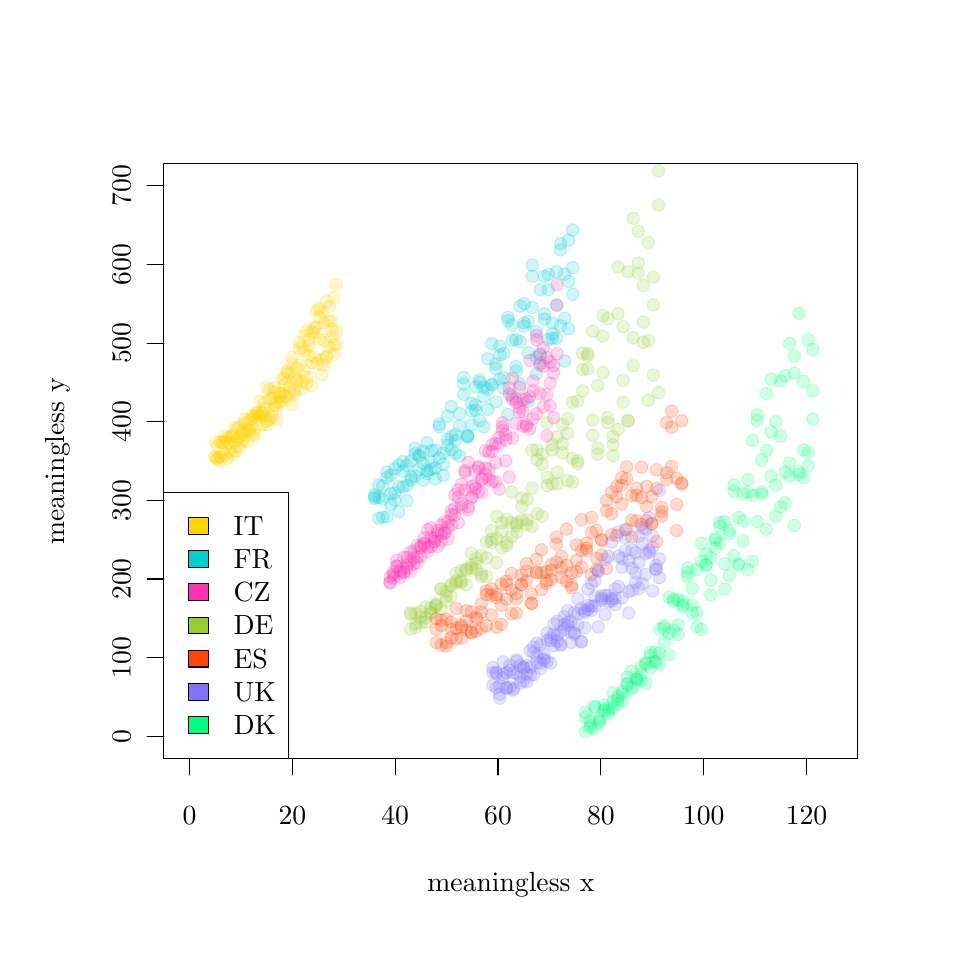
\begin{tikzpicture}[x=1pt,y=1pt]
\definecolor[named]{drawColor}{rgb}{0.00,0.00,0.00}
\definecolor[named]{fillColor}{rgb}{1.00,1.00,1.00}
\fill[color=fillColor,] (0,0) rectangle (325.21,325.21);
\begin{scope}
\path[clip] (  0.00,  0.00) rectangle (325.21,325.21);
\definecolor[named]{drawColor}{rgb}{0.18,0.00,0.33}
\definecolor[named]{drawColor}{rgb}{0.00,0.00,0.00}

\draw[color=drawColor,line cap=round,line join=round,fill opacity=0.00,] ( 58.49, 61.20) -- (281.44, 61.20);

\draw[color=drawColor,line cap=round,line join=round,fill opacity=0.00,] ( 58.49, 61.20) -- ( 58.49, 55.20);

\draw[color=drawColor,line cap=round,line join=round,fill opacity=0.00,] ( 95.65, 61.20) -- ( 95.65, 55.20);

\draw[color=drawColor,line cap=round,line join=round,fill opacity=0.00,] (132.80, 61.20) -- (132.80, 55.20);

\draw[color=drawColor,line cap=round,line join=round,fill opacity=0.00,] (169.96, 61.20) -- (169.96, 55.20);

\draw[color=drawColor,line cap=round,line join=round,fill opacity=0.00,] (207.12, 61.20) -- (207.12, 55.20);

\draw[color=drawColor,line cap=round,line join=round,fill opacity=0.00,] (244.28, 61.20) -- (244.28, 55.20);

\draw[color=drawColor,line cap=round,line join=round,fill opacity=0.00,] (281.44, 61.20) -- (281.44, 55.20);

\node[color=drawColor,anchor=base,inner sep=0pt, outer sep=0pt, scale=  1.00] at ( 58.49, 37.20) {0%
};

\node[color=drawColor,anchor=base,inner sep=0pt, outer sep=0pt, scale=  1.00] at ( 95.65, 37.20) {20%
};

\node[color=drawColor,anchor=base,inner sep=0pt, outer sep=0pt, scale=  1.00] at (132.80, 37.20) {40%
};

\node[color=drawColor,anchor=base,inner sep=0pt, outer sep=0pt, scale=  1.00] at (169.96, 37.20) {60%
};

\node[color=drawColor,anchor=base,inner sep=0pt, outer sep=0pt, scale=  1.00] at (207.12, 37.20) {80%
};

\node[color=drawColor,anchor=base,inner sep=0pt, outer sep=0pt, scale=  1.00] at (244.28, 37.20) {100%
};

\node[color=drawColor,anchor=base,inner sep=0pt, outer sep=0pt, scale=  1.00] at (281.44, 37.20) {120%
};

\draw[color=drawColor,line cap=round,line join=round,fill opacity=0.00,] ( 49.20, 69.16) -- ( 49.20,268.06);

\draw[color=drawColor,line cap=round,line join=round,fill opacity=0.00,] ( 49.20, 69.16) -- ( 43.20, 69.16);

\draw[color=drawColor,line cap=round,line join=round,fill opacity=0.00,] ( 49.20, 97.57) -- ( 43.20, 97.57);

\draw[color=drawColor,line cap=round,line join=round,fill opacity=0.00,] ( 49.20,125.99) -- ( 43.20,125.99);

\draw[color=drawColor,line cap=round,line join=round,fill opacity=0.00,] ( 49.20,154.40) -- ( 43.20,154.40);

\draw[color=drawColor,line cap=round,line join=round,fill opacity=0.00,] ( 49.20,182.81) -- ( 43.20,182.81);

\draw[color=drawColor,line cap=round,line join=round,fill opacity=0.00,] ( 49.20,211.23) -- ( 43.20,211.23);

\draw[color=drawColor,line cap=round,line join=round,fill opacity=0.00,] ( 49.20,239.64) -- ( 43.20,239.64);

\draw[color=drawColor,line cap=round,line join=round,fill opacity=0.00,] ( 49.20,268.06) -- ( 43.20,268.06);

\node[rotate= 90.00,color=drawColor,anchor=base,inner sep=0pt, outer sep=0pt, scale=  1.00] at ( 37.20, 69.16) {0%
};

\node[rotate= 90.00,color=drawColor,anchor=base,inner sep=0pt, outer sep=0pt, scale=  1.00] at ( 37.20, 97.57) {100%
};

\node[rotate= 90.00,color=drawColor,anchor=base,inner sep=0pt, outer sep=0pt, scale=  1.00] at ( 37.20,125.99) {200%
};

\node[rotate= 90.00,color=drawColor,anchor=base,inner sep=0pt, outer sep=0pt, scale=  1.00] at ( 37.20,154.40) {300%
};

\node[rotate= 90.00,color=drawColor,anchor=base,inner sep=0pt, outer sep=0pt, scale=  1.00] at ( 37.20,182.81) {400%
};

\node[rotate= 90.00,color=drawColor,anchor=base,inner sep=0pt, outer sep=0pt, scale=  1.00] at ( 37.20,211.23) {500%
};

\node[rotate= 90.00,color=drawColor,anchor=base,inner sep=0pt, outer sep=0pt, scale=  1.00] at ( 37.20,239.64) {600%
};

\node[rotate= 90.00,color=drawColor,anchor=base,inner sep=0pt, outer sep=0pt, scale=  1.00] at ( 37.20,268.06) {700%
};

\draw[color=drawColor,line cap=round,line join=round,fill opacity=0.00,] ( 49.20, 61.20) --
	(300.01, 61.20) --
	(300.01,276.01) --
	( 49.20,276.01) --
	( 49.20, 61.20);
\end{scope}
\begin{scope}
\path[clip] (  0.00,  0.00) rectangle (325.21,325.21);
\definecolor[named]{drawColor}{rgb}{0.18,0.00,0.33}
\definecolor[named]{drawColor}{rgb}{0.00,0.00,0.00}

\node[color=drawColor,anchor=base,inner sep=0pt, outer sep=0pt, scale=  1.00] at (174.61, 13.20) {meaningless x%
};

\node[rotate= 90.00,color=drawColor,anchor=base,inner sep=0pt, outer sep=0pt, scale=  1.00] at ( 13.20,168.61) {meaningless y%
};
\end{scope}
\begin{scope}
\path[clip] ( 49.20, 61.20) rectangle (300.01,276.01);
\definecolor[named]{drawColor}{rgb}{0.18,0.00,0.33}
\definecolor[named]{drawColor}{rgb}{1.00,0.84,0.00}
\definecolor[named]{fillColor}{rgb}{1.00,0.84,0.00}

\draw[color=drawColor,line cap=round,line join=round,fill=fillColor,fill opacity=0.19,draw opacity=0.19,] ( 67.78,170.07) circle (  2.25);

\draw[color=drawColor,line cap=round,line join=round,fill=fillColor,fill opacity=0.19,draw opacity=0.19,] ( 68.67,169.52) circle (  2.25);

\draw[color=drawColor,line cap=round,line join=round,fill=fillColor,fill opacity=0.19,draw opacity=0.19,] ( 69.57,170.04) circle (  2.25);

\draw[color=drawColor,line cap=round,line join=round,fill=fillColor,fill opacity=0.19,draw opacity=0.19,] ( 70.46,171.54) circle (  2.25);

\draw[color=drawColor,line cap=round,line join=round,fill=fillColor,fill opacity=0.19,draw opacity=0.19,] ( 71.36,175.95) circle (  2.25);

\draw[color=drawColor,line cap=round,line join=round,fill=fillColor,fill opacity=0.19,draw opacity=0.19,] ( 72.25,176.72) circle (  2.25);

\draw[color=drawColor,line cap=round,line join=round,fill=fillColor,fill opacity=0.19,draw opacity=0.19,] ( 73.14,171.70) circle (  2.25);

\draw[color=drawColor,line cap=round,line join=round,fill=fillColor,fill opacity=0.19,draw opacity=0.19,] ( 74.04,177.81) circle (  2.25);

\draw[color=drawColor,line cap=round,line join=round,fill=fillColor,fill opacity=0.19,draw opacity=0.19,] ( 74.93,180.69) circle (  2.25);

\draw[color=drawColor,line cap=round,line join=round,fill=fillColor,fill opacity=0.19,draw opacity=0.19,] ( 75.83,176.29) circle (  2.25);

\draw[color=drawColor,line cap=round,line join=round,fill=fillColor,fill opacity=0.19,draw opacity=0.19,] ( 76.72,181.26) circle (  2.25);

\draw[color=drawColor,line cap=round,line join=round,fill=fillColor,fill opacity=0.19,draw opacity=0.19,] ( 77.62,178.55) circle (  2.25);

\draw[color=drawColor,line cap=round,line join=round,fill=fillColor,fill opacity=0.19,draw opacity=0.19,] ( 78.51,182.45) circle (  2.25);

\draw[color=drawColor,line cap=round,line join=round,fill=fillColor,fill opacity=0.19,draw opacity=0.19,] ( 79.40,181.91) circle (  2.25);

\draw[color=drawColor,line cap=round,line join=round,fill=fillColor,fill opacity=0.19,draw opacity=0.19,] ( 80.30,179.85) circle (  2.25);

\draw[color=drawColor,line cap=round,line join=round,fill=fillColor,fill opacity=0.19,draw opacity=0.19,] ( 81.19,185.24) circle (  2.25);

\draw[color=drawColor,line cap=round,line join=round,fill=fillColor,fill opacity=0.19,draw opacity=0.19,] ( 82.09,184.92) circle (  2.25);

\draw[color=drawColor,line cap=round,line join=round,fill=fillColor,fill opacity=0.19,draw opacity=0.19,] ( 82.98,185.23) circle (  2.25);

\draw[color=drawColor,line cap=round,line join=round,fill=fillColor,fill opacity=0.19,draw opacity=0.19,] ( 83.87,185.23) circle (  2.25);

\draw[color=drawColor,line cap=round,line join=round,fill=fillColor,fill opacity=0.19,draw opacity=0.19,] ( 84.77,186.27) circle (  2.25);

\draw[color=drawColor,line cap=round,line join=round,fill=fillColor,fill opacity=0.19,draw opacity=0.19,] ( 85.66,189.92) circle (  2.25);

\draw[color=drawColor,line cap=round,line join=round,fill=fillColor,fill opacity=0.19,draw opacity=0.19,] ( 86.56,195.08) circle (  2.25);

\draw[color=drawColor,line cap=round,line join=round,fill=fillColor,fill opacity=0.19,draw opacity=0.19,] ( 87.45,183.59) circle (  2.25);

\draw[color=drawColor,line cap=round,line join=round,fill=fillColor,fill opacity=0.19,draw opacity=0.19,] ( 88.35,191.36) circle (  2.25);

\draw[color=drawColor,line cap=round,line join=round,fill=fillColor,fill opacity=0.19,draw opacity=0.19,] ( 89.24,195.07) circle (  2.25);

\draw[color=drawColor,line cap=round,line join=round,fill=fillColor,fill opacity=0.19,draw opacity=0.19,] ( 90.13,188.45) circle (  2.25);

\draw[color=drawColor,line cap=round,line join=round,fill=fillColor,fill opacity=0.19,draw opacity=0.19,] ( 91.03,193.10) circle (  2.25);

\draw[color=drawColor,line cap=round,line join=round,fill=fillColor,fill opacity=0.19,draw opacity=0.19,] ( 91.92,198.51) circle (  2.25);

\draw[color=drawColor,line cap=round,line join=round,fill=fillColor,fill opacity=0.19,draw opacity=0.19,] ( 92.82,196.27) circle (  2.25);

\draw[color=drawColor,line cap=round,line join=round,fill=fillColor,fill opacity=0.19,draw opacity=0.19,] ( 93.71,191.59) circle (  2.25);

\draw[color=drawColor,line cap=round,line join=round,fill=fillColor,fill opacity=0.19,draw opacity=0.19,] ( 94.61,193.56) circle (  2.25);

\draw[color=drawColor,line cap=round,line join=round,fill=fillColor,fill opacity=0.19,draw opacity=0.19,] ( 95.50,206.14) circle (  2.25);

\draw[color=drawColor,line cap=round,line join=round,fill=fillColor,fill opacity=0.19,draw opacity=0.19,] ( 96.39,192.68) circle (  2.25);

\draw[color=drawColor,line cap=round,line join=round,fill=fillColor,fill opacity=0.19,draw opacity=0.19,] ( 97.29,197.94) circle (  2.25);

\draw[color=drawColor,line cap=round,line join=round,fill=fillColor,fill opacity=0.19,draw opacity=0.19,] ( 98.18,209.29) circle (  2.25);

\draw[color=drawColor,line cap=round,line join=round,fill=fillColor,fill opacity=0.19,draw opacity=0.19,] ( 99.08,194.66) circle (  2.25);

\draw[color=drawColor,line cap=round,line join=round,fill=fillColor,fill opacity=0.19,draw opacity=0.19,] ( 99.97,208.52) circle (  2.25);

\draw[color=drawColor,line cap=round,line join=round,fill=fillColor,fill opacity=0.19,draw opacity=0.19,] (100.86,198.95) circle (  2.25);

\draw[color=drawColor,line cap=round,line join=round,fill=fillColor,fill opacity=0.19,draw opacity=0.19,] (101.76,206.67) circle (  2.25);

\draw[color=drawColor,line cap=round,line join=round,fill=fillColor,fill opacity=0.19,draw opacity=0.19,] (102.65,195.77) circle (  2.25);

\draw[color=drawColor,line cap=round,line join=round,fill=fillColor,fill opacity=0.19,draw opacity=0.19,] (103.55,216.74) circle (  2.25);

\draw[color=drawColor,line cap=round,line join=round,fill=fillColor,fill opacity=0.19,draw opacity=0.19,] (104.44,223.15) circle (  2.25);

\draw[color=drawColor,line cap=round,line join=round,fill=fillColor,fill opacity=0.19,draw opacity=0.19,] (105.34,220.64) circle (  2.25);

\draw[color=drawColor,line cap=round,line join=round,fill=fillColor,fill opacity=0.19,draw opacity=0.19,] (106.23,205.27) circle (  2.25);

\draw[color=drawColor,line cap=round,line join=round,fill=fillColor,fill opacity=0.19,draw opacity=0.19,] (107.12,218.51) circle (  2.25);

\draw[color=drawColor,line cap=round,line join=round,fill=fillColor,fill opacity=0.19,draw opacity=0.19,] (108.02,206.09) circle (  2.25);

\draw[color=drawColor,line cap=round,line join=round,fill=fillColor,fill opacity=0.19,draw opacity=0.19,] (108.91,219.19) circle (  2.25);

\draw[color=drawColor,line cap=round,line join=round,fill=fillColor,fill opacity=0.19,draw opacity=0.19,] (109.81,213.53) circle (  2.25);

\draw[color=drawColor,line cap=round,line join=round,fill=fillColor,fill opacity=0.19,draw opacity=0.19,] (110.70,207.11) circle (  2.25);

\draw[color=drawColor,line cap=round,line join=round,fill=fillColor,fill opacity=0.19,draw opacity=0.19,] (111.60,210.53) circle (  2.25);

\draw[color=drawColor,line cap=round,line join=round,fill=fillColor,fill opacity=0.19,draw opacity=0.19,] ( 67.78,175.54) circle (  2.25);

\draw[color=drawColor,line cap=round,line join=round,fill=fillColor,fill opacity=0.19,draw opacity=0.19,] ( 68.67,174.10) circle (  2.25);

\draw[color=drawColor,line cap=round,line join=round,fill=fillColor,fill opacity=0.19,draw opacity=0.19,] ( 69.57,168.60) circle (  2.25);

\draw[color=drawColor,line cap=round,line join=round,fill=fillColor,fill opacity=0.19,draw opacity=0.19,] ( 70.46,175.23) circle (  2.25);

\draw[color=drawColor,line cap=round,line join=round,fill=fillColor,fill opacity=0.19,draw opacity=0.19,] ( 71.36,177.57) circle (  2.25);

\draw[color=drawColor,line cap=round,line join=round,fill=fillColor,fill opacity=0.19,draw opacity=0.19,] ( 72.25,175.36) circle (  2.25);

\draw[color=drawColor,line cap=round,line join=round,fill=fillColor,fill opacity=0.19,draw opacity=0.19,] ( 73.14,175.00) circle (  2.25);

\draw[color=drawColor,line cap=round,line join=round,fill=fillColor,fill opacity=0.19,draw opacity=0.19,] ( 74.04,177.58) circle (  2.25);

\draw[color=drawColor,line cap=round,line join=round,fill=fillColor,fill opacity=0.19,draw opacity=0.19,] ( 74.93,172.14) circle (  2.25);

\draw[color=drawColor,line cap=round,line join=round,fill=fillColor,fill opacity=0.19,draw opacity=0.19,] ( 75.83,173.71) circle (  2.25);

\draw[color=drawColor,line cap=round,line join=round,fill=fillColor,fill opacity=0.19,draw opacity=0.19,] ( 76.72,173.63) circle (  2.25);

\draw[color=drawColor,line cap=round,line join=round,fill=fillColor,fill opacity=0.19,draw opacity=0.19,] ( 77.62,179.32) circle (  2.25);

\draw[color=drawColor,line cap=round,line join=round,fill=fillColor,fill opacity=0.19,draw opacity=0.19,] ( 78.51,177.97) circle (  2.25);

\draw[color=drawColor,line cap=round,line join=round,fill=fillColor,fill opacity=0.19,draw opacity=0.19,] ( 79.40,175.60) circle (  2.25);

\draw[color=drawColor,line cap=round,line join=round,fill=fillColor,fill opacity=0.19,draw opacity=0.19,] ( 80.30,183.55) circle (  2.25);

\draw[color=drawColor,line cap=round,line join=round,fill=fillColor,fill opacity=0.19,draw opacity=0.19,] ( 81.19,177.85) circle (  2.25);

\draw[color=drawColor,line cap=round,line join=round,fill=fillColor,fill opacity=0.19,draw opacity=0.19,] ( 82.09,180.07) circle (  2.25);

\draw[color=drawColor,line cap=round,line join=round,fill=fillColor,fill opacity=0.19,draw opacity=0.19,] ( 82.98,186.14) circle (  2.25);

\draw[color=drawColor,line cap=round,line join=round,fill=fillColor,fill opacity=0.19,draw opacity=0.19,] ( 83.87,190.21) circle (  2.25);

\draw[color=drawColor,line cap=round,line join=round,fill=fillColor,fill opacity=0.19,draw opacity=0.19,] ( 84.77,185.80) circle (  2.25);

\draw[color=drawColor,line cap=round,line join=round,fill=fillColor,fill opacity=0.19,draw opacity=0.19,] ( 85.66,184.69) circle (  2.25);

\draw[color=drawColor,line cap=round,line join=round,fill=fillColor,fill opacity=0.19,draw opacity=0.19,] ( 86.56,181.69) circle (  2.25);

\draw[color=drawColor,line cap=round,line join=round,fill=fillColor,fill opacity=0.19,draw opacity=0.19,] ( 87.45,194.35) circle (  2.25);

\draw[color=drawColor,line cap=round,line join=round,fill=fillColor,fill opacity=0.19,draw opacity=0.19,] ( 88.35,184.59) circle (  2.25);

\draw[color=drawColor,line cap=round,line join=round,fill=fillColor,fill opacity=0.19,draw opacity=0.19,] ( 89.24,188.65) circle (  2.25);

\draw[color=drawColor,line cap=round,line join=round,fill=fillColor,fill opacity=0.19,draw opacity=0.19,] ( 90.13,183.54) circle (  2.25);

\draw[color=drawColor,line cap=round,line join=round,fill=fillColor,fill opacity=0.19,draw opacity=0.19,] ( 91.03,189.81) circle (  2.25);

\draw[color=drawColor,line cap=round,line join=round,fill=fillColor,fill opacity=0.19,draw opacity=0.19,] ( 91.92,193.02) circle (  2.25);

\draw[color=drawColor,line cap=round,line join=round,fill=fillColor,fill opacity=0.19,draw opacity=0.19,] ( 92.82,198.23) circle (  2.25);

\draw[color=drawColor,line cap=round,line join=round,fill=fillColor,fill opacity=0.19,draw opacity=0.19,] ( 93.71,201.16) circle (  2.25);

\draw[color=drawColor,line cap=round,line join=round,fill=fillColor,fill opacity=0.19,draw opacity=0.19,] ( 94.61,200.42) circle (  2.25);

\draw[color=drawColor,line cap=round,line join=round,fill=fillColor,fill opacity=0.19,draw opacity=0.19,] ( 95.50,189.06) circle (  2.25);

\draw[color=drawColor,line cap=round,line join=round,fill=fillColor,fill opacity=0.19,draw opacity=0.19,] ( 96.39,193.97) circle (  2.25);

\draw[color=drawColor,line cap=round,line join=round,fill=fillColor,fill opacity=0.19,draw opacity=0.19,] ( 97.29,197.34) circle (  2.25);

\draw[color=drawColor,line cap=round,line join=round,fill=fillColor,fill opacity=0.19,draw opacity=0.19,] ( 98.18,211.56) circle (  2.25);

\draw[color=drawColor,line cap=round,line join=round,fill=fillColor,fill opacity=0.19,draw opacity=0.19,] ( 99.08,197.24) circle (  2.25);

\draw[color=drawColor,line cap=round,line join=round,fill=fillColor,fill opacity=0.19,draw opacity=0.19,] ( 99.97,214.05) circle (  2.25);

\draw[color=drawColor,line cap=round,line join=round,fill=fillColor,fill opacity=0.19,draw opacity=0.19,] (100.86,215.81) circle (  2.25);

\draw[color=drawColor,line cap=round,line join=round,fill=fillColor,fill opacity=0.19,draw opacity=0.19,] (101.76,212.45) circle (  2.25);

\draw[color=drawColor,line cap=round,line join=round,fill=fillColor,fill opacity=0.19,draw opacity=0.19,] (102.65,215.21) circle (  2.25);

\draw[color=drawColor,line cap=round,line join=round,fill=fillColor,fill opacity=0.19,draw opacity=0.19,] (103.55,206.27) circle (  2.25);

\draw[color=drawColor,line cap=round,line join=round,fill=fillColor,fill opacity=0.19,draw opacity=0.19,] (104.44,203.85) circle (  2.25);

\draw[color=drawColor,line cap=round,line join=round,fill=fillColor,fill opacity=0.19,draw opacity=0.19,] (105.34,212.64) circle (  2.25);

\draw[color=drawColor,line cap=round,line join=round,fill=fillColor,fill opacity=0.19,draw opacity=0.19,] (106.23,199.82) circle (  2.25);

\draw[color=drawColor,line cap=round,line join=round,fill=fillColor,fill opacity=0.19,draw opacity=0.19,] (107.12,212.15) circle (  2.25);

\draw[color=drawColor,line cap=round,line join=round,fill=fillColor,fill opacity=0.19,draw opacity=0.19,] (108.02,226.32) circle (  2.25);

\draw[color=drawColor,line cap=round,line join=round,fill=fillColor,fill opacity=0.19,draw opacity=0.19,] (108.91,224.45) circle (  2.25);

\draw[color=drawColor,line cap=round,line join=round,fill=fillColor,fill opacity=0.19,draw opacity=0.19,] (109.81,216.16) circle (  2.25);

\draw[color=drawColor,line cap=round,line join=round,fill=fillColor,fill opacity=0.19,draw opacity=0.19,] (110.70,227.70) circle (  2.25);

\draw[color=drawColor,line cap=round,line join=round,fill=fillColor,fill opacity=0.19,draw opacity=0.19,] (111.60,215.41) circle (  2.25);

\draw[color=drawColor,line cap=round,line join=round,fill=fillColor,fill opacity=0.19,draw opacity=0.19,] ( 67.78,170.07) circle (  2.25);

\draw[color=drawColor,line cap=round,line join=round,fill=fillColor,fill opacity=0.19,draw opacity=0.19,] ( 68.67,169.40) circle (  2.25);

\draw[color=drawColor,line cap=round,line join=round,fill=fillColor,fill opacity=0.19,draw opacity=0.19,] ( 69.57,175.55) circle (  2.25);

\draw[color=drawColor,line cap=round,line join=round,fill=fillColor,fill opacity=0.19,draw opacity=0.19,] ( 70.46,175.35) circle (  2.25);

\draw[color=drawColor,line cap=round,line join=round,fill=fillColor,fill opacity=0.19,draw opacity=0.19,] ( 71.36,171.02) circle (  2.25);

\draw[color=drawColor,line cap=round,line join=round,fill=fillColor,fill opacity=0.19,draw opacity=0.19,] ( 72.25,169.64) circle (  2.25);

\draw[color=drawColor,line cap=round,line join=round,fill=fillColor,fill opacity=0.19,draw opacity=0.19,] ( 73.14,177.35) circle (  2.25);

\draw[color=drawColor,line cap=round,line join=round,fill=fillColor,fill opacity=0.19,draw opacity=0.19,] ( 74.04,170.91) circle (  2.25);

\draw[color=drawColor,line cap=round,line join=round,fill=fillColor,fill opacity=0.19,draw opacity=0.19,] ( 74.93,175.63) circle (  2.25);

\draw[color=drawColor,line cap=round,line join=round,fill=fillColor,fill opacity=0.19,draw opacity=0.19,] ( 75.83,180.48) circle (  2.25);

\draw[color=drawColor,line cap=round,line join=round,fill=fillColor,fill opacity=0.19,draw opacity=0.19,] ( 76.72,177.29) circle (  2.25);

\draw[color=drawColor,line cap=round,line join=round,fill=fillColor,fill opacity=0.19,draw opacity=0.19,] ( 77.62,176.08) circle (  2.25);

\draw[color=drawColor,line cap=round,line join=round,fill=fillColor,fill opacity=0.19,draw opacity=0.19,] ( 78.51,183.73) circle (  2.25);

\draw[color=drawColor,line cap=round,line join=round,fill=fillColor,fill opacity=0.19,draw opacity=0.19,] ( 79.40,179.65) circle (  2.25);

\draw[color=drawColor,line cap=round,line join=round,fill=fillColor,fill opacity=0.19,draw opacity=0.19,] ( 80.30,180.93) circle (  2.25);

\draw[color=drawColor,line cap=round,line join=round,fill=fillColor,fill opacity=0.19,draw opacity=0.19,] ( 81.19,183.94) circle (  2.25);

\draw[color=drawColor,line cap=round,line join=round,fill=fillColor,fill opacity=0.19,draw opacity=0.19,] ( 82.09,178.21) circle (  2.25);

\draw[color=drawColor,line cap=round,line join=round,fill=fillColor,fill opacity=0.19,draw opacity=0.19,] ( 82.98,185.91) circle (  2.25);

\draw[color=drawColor,line cap=round,line join=round,fill=fillColor,fill opacity=0.19,draw opacity=0.19,] ( 83.87,184.35) circle (  2.25);

\draw[color=drawColor,line cap=round,line join=round,fill=fillColor,fill opacity=0.19,draw opacity=0.19,] ( 84.77,181.69) circle (  2.25);

\draw[color=drawColor,line cap=round,line join=round,fill=fillColor,fill opacity=0.19,draw opacity=0.19,] ( 85.66,187.52) circle (  2.25);

\draw[color=drawColor,line cap=round,line join=round,fill=fillColor,fill opacity=0.19,draw opacity=0.19,] ( 86.56,182.93) circle (  2.25);

\draw[color=drawColor,line cap=round,line join=round,fill=fillColor,fill opacity=0.19,draw opacity=0.19,] ( 87.45,190.97) circle (  2.25);

\draw[color=drawColor,line cap=round,line join=round,fill=fillColor,fill opacity=0.19,draw opacity=0.19,] ( 88.35,186.04) circle (  2.25);

\draw[color=drawColor,line cap=round,line join=round,fill=fillColor,fill opacity=0.19,draw opacity=0.19,] ( 89.24,193.40) circle (  2.25);

\draw[color=drawColor,line cap=round,line join=round,fill=fillColor,fill opacity=0.19,draw opacity=0.19,] ( 90.13,190.07) circle (  2.25);

\draw[color=drawColor,line cap=round,line join=round,fill=fillColor,fill opacity=0.19,draw opacity=0.19,] ( 91.03,192.01) circle (  2.25);

\draw[color=drawColor,line cap=round,line join=round,fill=fillColor,fill opacity=0.19,draw opacity=0.19,] ( 91.92,190.34) circle (  2.25);

\draw[color=drawColor,line cap=round,line join=round,fill=fillColor,fill opacity=0.19,draw opacity=0.19,] ( 92.82,192.18) circle (  2.25);

\draw[color=drawColor,line cap=round,line join=round,fill=fillColor,fill opacity=0.19,draw opacity=0.19,] ( 93.71,200.78) circle (  2.25);

\draw[color=drawColor,line cap=round,line join=round,fill=fillColor,fill opacity=0.19,draw opacity=0.19,] ( 94.61,195.23) circle (  2.25);

\draw[color=drawColor,line cap=round,line join=round,fill=fillColor,fill opacity=0.19,draw opacity=0.19,] ( 95.50,203.62) circle (  2.25);

\draw[color=drawColor,line cap=round,line join=round,fill=fillColor,fill opacity=0.19,draw opacity=0.19,] ( 96.39,198.81) circle (  2.25);

\draw[color=drawColor,line cap=round,line join=round,fill=fillColor,fill opacity=0.19,draw opacity=0.19,] ( 97.29,202.13) circle (  2.25);

\draw[color=drawColor,line cap=round,line join=round,fill=fillColor,fill opacity=0.19,draw opacity=0.19,] ( 98.18,203.30) circle (  2.25);

\draw[color=drawColor,line cap=round,line join=round,fill=fillColor,fill opacity=0.19,draw opacity=0.19,] ( 99.08,209.61) circle (  2.25);

\draw[color=drawColor,line cap=round,line join=round,fill=fillColor,fill opacity=0.19,draw opacity=0.19,] ( 99.97,201.46) circle (  2.25);

\draw[color=drawColor,line cap=round,line join=round,fill=fillColor,fill opacity=0.19,draw opacity=0.19,] (100.86,196.83) circle (  2.25);

\draw[color=drawColor,line cap=round,line join=round,fill=fillColor,fill opacity=0.19,draw opacity=0.19,] (101.76,210.24) circle (  2.25);

\draw[color=drawColor,line cap=round,line join=round,fill=fillColor,fill opacity=0.19,draw opacity=0.19,] (102.65,204.15) circle (  2.25);

\draw[color=drawColor,line cap=round,line join=round,fill=fillColor,fill opacity=0.19,draw opacity=0.19,] (103.55,215.00) circle (  2.25);

\draw[color=drawColor,line cap=round,line join=round,fill=fillColor,fill opacity=0.19,draw opacity=0.19,] (104.44,217.01) circle (  2.25);

\draw[color=drawColor,line cap=round,line join=round,fill=fillColor,fill opacity=0.19,draw opacity=0.19,] (105.34,223.69) circle (  2.25);

\draw[color=drawColor,line cap=round,line join=round,fill=fillColor,fill opacity=0.19,draw opacity=0.19,] (106.23,222.64) circle (  2.25);

\draw[color=drawColor,line cap=round,line join=round,fill=fillColor,fill opacity=0.19,draw opacity=0.19,] (107.12,203.27) circle (  2.25);

\draw[color=drawColor,line cap=round,line join=round,fill=fillColor,fill opacity=0.19,draw opacity=0.19,] (108.02,206.61) circle (  2.25);

\draw[color=drawColor,line cap=round,line join=round,fill=fillColor,fill opacity=0.19,draw opacity=0.19,] (108.91,209.73) circle (  2.25);

\draw[color=drawColor,line cap=round,line join=round,fill=fillColor,fill opacity=0.19,draw opacity=0.19,] (109.81,219.21) circle (  2.25);

\draw[color=drawColor,line cap=round,line join=round,fill=fillColor,fill opacity=0.19,draw opacity=0.19,] (110.70,210.70) circle (  2.25);

\draw[color=drawColor,line cap=round,line join=round,fill=fillColor,fill opacity=0.19,draw opacity=0.19,] (111.60,232.38) circle (  2.25);
\definecolor[named]{drawColor}{rgb}{0.00,0.81,0.82}
\definecolor[named]{fillColor}{rgb}{0.00,0.81,0.82}

\draw[color=drawColor,line cap=round,line join=round,fill=fillColor,fill opacity=0.19,draw opacity=0.19,] (125.37,155.16) circle (  2.25);

\draw[color=drawColor,line cap=round,line join=round,fill=fillColor,fill opacity=0.19,draw opacity=0.19,] (126.83,159.99) circle (  2.25);

\draw[color=drawColor,line cap=round,line join=round,fill=fillColor,fill opacity=0.19,draw opacity=0.19,] (128.29,159.59) circle (  2.25);

\draw[color=drawColor,line cap=round,line join=round,fill=fillColor,fill opacity=0.19,draw opacity=0.19,] (129.75,148.39) circle (  2.25);

\draw[color=drawColor,line cap=round,line join=round,fill=fillColor,fill opacity=0.19,draw opacity=0.19,] (131.21,163.44) circle (  2.25);

\draw[color=drawColor,line cap=round,line join=round,fill=fillColor,fill opacity=0.19,draw opacity=0.19,] (132.68,154.58) circle (  2.25);

\draw[color=drawColor,line cap=round,line join=round,fill=fillColor,fill opacity=0.19,draw opacity=0.19,] (134.14,150.31) circle (  2.25);

\draw[color=drawColor,line cap=round,line join=round,fill=fillColor,fill opacity=0.19,draw opacity=0.19,] (135.60,164.93) circle (  2.25);

\draw[color=drawColor,line cap=round,line join=round,fill=fillColor,fill opacity=0.19,draw opacity=0.19,] (137.06,154.27) circle (  2.25);

\draw[color=drawColor,line cap=round,line join=round,fill=fillColor,fill opacity=0.19,draw opacity=0.19,] (138.52,162.86) circle (  2.25);

\draw[color=drawColor,line cap=round,line join=round,fill=fillColor,fill opacity=0.19,draw opacity=0.19,] (139.98,171.25) circle (  2.25);

\draw[color=drawColor,line cap=round,line join=round,fill=fillColor,fill opacity=0.19,draw opacity=0.19,] (141.44,170.30) circle (  2.25);

\draw[color=drawColor,line cap=round,line join=round,fill=fillColor,fill opacity=0.19,draw opacity=0.19,] (142.90,167.74) circle (  2.25);

\draw[color=drawColor,line cap=round,line join=round,fill=fillColor,fill opacity=0.19,draw opacity=0.19,] (144.36,175.26) circle (  2.25);

\draw[color=drawColor,line cap=round,line join=round,fill=fillColor,fill opacity=0.19,draw opacity=0.19,] (145.82,165.65) circle (  2.25);

\draw[color=drawColor,line cap=round,line join=round,fill=fillColor,fill opacity=0.19,draw opacity=0.19,] (147.28,162.24) circle (  2.25);

\draw[color=drawColor,line cap=round,line join=round,fill=fillColor,fill opacity=0.19,draw opacity=0.19,] (148.74,180.98) circle (  2.25);

\draw[color=drawColor,line cap=round,line join=round,fill=fillColor,fill opacity=0.19,draw opacity=0.19,] (150.20,163.42) circle (  2.25);

\draw[color=drawColor,line cap=round,line join=round,fill=fillColor,fill opacity=0.19,draw opacity=0.19,] (151.66,176.50) circle (  2.25);

\draw[color=drawColor,line cap=round,line join=round,fill=fillColor,fill opacity=0.19,draw opacity=0.19,] (153.12,177.49) circle (  2.25);

\draw[color=drawColor,line cap=round,line join=round,fill=fillColor,fill opacity=0.19,draw opacity=0.19,] (154.58,176.08) circle (  2.25);

\draw[color=drawColor,line cap=round,line join=round,fill=fillColor,fill opacity=0.19,draw opacity=0.19,] (156.04,185.71) circle (  2.25);

\draw[color=drawColor,line cap=round,line join=round,fill=fillColor,fill opacity=0.19,draw opacity=0.19,] (157.50,196.39) circle (  2.25);

\draw[color=drawColor,line cap=round,line join=round,fill=fillColor,fill opacity=0.19,draw opacity=0.19,] (158.96,177.37) circle (  2.25);

\draw[color=drawColor,line cap=round,line join=round,fill=fillColor,fill opacity=0.19,draw opacity=0.19,] (160.42,181.74) circle (  2.25);

\draw[color=drawColor,line cap=round,line join=round,fill=fillColor,fill opacity=0.19,draw opacity=0.19,] (161.88,186.95) circle (  2.25);

\draw[color=drawColor,line cap=round,line join=round,fill=fillColor,fill opacity=0.19,draw opacity=0.19,] (163.34,183.23) circle (  2.25);

\draw[color=drawColor,line cap=round,line join=round,fill=fillColor,fill opacity=0.19,draw opacity=0.19,] (164.80,195.31) circle (  2.25);

\draw[color=drawColor,line cap=round,line join=round,fill=fillColor,fill opacity=0.19,draw opacity=0.19,] (166.26,187.28) circle (  2.25);

\draw[color=drawColor,line cap=round,line join=round,fill=fillColor,fill opacity=0.19,draw opacity=0.19,] (167.72,210.98) circle (  2.25);

\draw[color=drawColor,line cap=round,line join=round,fill=fillColor,fill opacity=0.19,draw opacity=0.19,] (169.18,189.96) circle (  2.25);

\draw[color=drawColor,line cap=round,line join=round,fill=fillColor,fill opacity=0.19,draw opacity=0.19,] (170.64,206.93) circle (  2.25);

\draw[color=drawColor,line cap=round,line join=round,fill=fillColor,fill opacity=0.19,draw opacity=0.19,] (172.10,207.52) circle (  2.25);

\draw[color=drawColor,line cap=round,line join=round,fill=fillColor,fill opacity=0.19,draw opacity=0.19,] (173.56,220.51) circle (  2.25);

\draw[color=drawColor,line cap=round,line join=round,fill=fillColor,fill opacity=0.19,draw opacity=0.19,] (175.02,191.97) circle (  2.25);

\draw[color=drawColor,line cap=round,line join=round,fill=fillColor,fill opacity=0.19,draw opacity=0.19,] (176.49,202.78) circle (  2.25);

\draw[color=drawColor,line cap=round,line join=round,fill=fillColor,fill opacity=0.19,draw opacity=0.19,] (177.95,211.80) circle (  2.25);

\draw[color=drawColor,line cap=round,line join=round,fill=fillColor,fill opacity=0.19,draw opacity=0.19,] (179.41,225.48) circle (  2.25);

\draw[color=drawColor,line cap=round,line join=round,fill=fillColor,fill opacity=0.19,draw opacity=0.19,] (180.87,207.75) circle (  2.25);

\draw[color=drawColor,line cap=round,line join=round,fill=fillColor,fill opacity=0.19,draw opacity=0.19,] (182.33,235.42) circle (  2.25);

\draw[color=drawColor,line cap=round,line join=round,fill=fillColor,fill opacity=0.19,draw opacity=0.19,] (183.79,206.00) circle (  2.25);

\draw[color=drawColor,line cap=round,line join=round,fill=fillColor,fill opacity=0.19,draw opacity=0.19,] (185.25,207.39) circle (  2.25);

\draw[color=drawColor,line cap=round,line join=round,fill=fillColor,fill opacity=0.19,draw opacity=0.19,] (186.71,219.88) circle (  2.25);

\draw[color=drawColor,line cap=round,line join=round,fill=fillColor,fill opacity=0.19,draw opacity=0.19,] (188.17,212.49) circle (  2.25);

\draw[color=drawColor,line cap=round,line join=round,fill=fillColor,fill opacity=0.19,draw opacity=0.19,] (189.63,213.00) circle (  2.25);

\draw[color=drawColor,line cap=round,line join=round,fill=fillColor,fill opacity=0.19,draw opacity=0.19,] (191.09,225.01) circle (  2.25);

\draw[color=drawColor,line cap=round,line join=round,fill=fillColor,fill opacity=0.19,draw opacity=0.19,] (192.55,244.88) circle (  2.25);

\draw[color=drawColor,line cap=round,line join=round,fill=fillColor,fill opacity=0.19,draw opacity=0.19,] (194.01,220.23) circle (  2.25);

\draw[color=drawColor,line cap=round,line join=round,fill=fillColor,fill opacity=0.19,draw opacity=0.19,] (195.47,248.45) circle (  2.25);

\draw[color=drawColor,line cap=round,line join=round,fill=fillColor,fill opacity=0.19,draw opacity=0.19,] (196.93,228.87) circle (  2.25);

\draw[color=drawColor,line cap=round,line join=round,fill=fillColor,fill opacity=0.19,draw opacity=0.19,] (125.37,156.42) circle (  2.25);

\draw[color=drawColor,line cap=round,line join=round,fill=fillColor,fill opacity=0.19,draw opacity=0.19,] (126.83,147.95) circle (  2.25);

\draw[color=drawColor,line cap=round,line join=round,fill=fillColor,fill opacity=0.19,draw opacity=0.19,] (128.29,154.79) circle (  2.25);

\draw[color=drawColor,line cap=round,line join=round,fill=fillColor,fill opacity=0.19,draw opacity=0.19,] (129.75,162.62) circle (  2.25);

\draw[color=drawColor,line cap=round,line join=round,fill=fillColor,fill opacity=0.19,draw opacity=0.19,] (131.21,152.97) circle (  2.25);

\draw[color=drawColor,line cap=round,line join=round,fill=fillColor,fill opacity=0.19,draw opacity=0.19,] (132.68,165.83) circle (  2.25);

\draw[color=drawColor,line cap=round,line join=round,fill=fillColor,fill opacity=0.19,draw opacity=0.19,] (134.14,159.38) circle (  2.25);

\draw[color=drawColor,line cap=round,line join=round,fill=fillColor,fill opacity=0.19,draw opacity=0.19,] (135.60,168.44) circle (  2.25);

\draw[color=drawColor,line cap=round,line join=round,fill=fillColor,fill opacity=0.19,draw opacity=0.19,] (137.06,159.79) circle (  2.25);

\draw[color=drawColor,line cap=round,line join=round,fill=fillColor,fill opacity=0.19,draw opacity=0.19,] (138.52,168.67) circle (  2.25);

\draw[color=drawColor,line cap=round,line join=round,fill=fillColor,fill opacity=0.19,draw opacity=0.19,] (139.98,163.14) circle (  2.25);

\draw[color=drawColor,line cap=round,line join=round,fill=fillColor,fill opacity=0.19,draw opacity=0.19,] (141.44,170.67) circle (  2.25);

\draw[color=drawColor,line cap=round,line join=round,fill=fillColor,fill opacity=0.19,draw opacity=0.19,] (142.90,172.07) circle (  2.25);

\draw[color=drawColor,line cap=round,line join=round,fill=fillColor,fill opacity=0.19,draw opacity=0.19,] (144.36,164.09) circle (  2.25);

\draw[color=drawColor,line cap=round,line join=round,fill=fillColor,fill opacity=0.19,draw opacity=0.19,] (145.82,172.40) circle (  2.25);

\draw[color=drawColor,line cap=round,line join=round,fill=fillColor,fill opacity=0.19,draw opacity=0.19,] (147.28,166.10) circle (  2.25);

\draw[color=drawColor,line cap=round,line join=round,fill=fillColor,fill opacity=0.19,draw opacity=0.19,] (148.74,181.90) circle (  2.25);

\draw[color=drawColor,line cap=round,line join=round,fill=fillColor,fill opacity=0.19,draw opacity=0.19,] (150.20,167.38) circle (  2.25);

\draw[color=drawColor,line cap=round,line join=round,fill=fillColor,fill opacity=0.19,draw opacity=0.19,] (151.66,174.23) circle (  2.25);

\draw[color=drawColor,line cap=round,line join=round,fill=fillColor,fill opacity=0.19,draw opacity=0.19,] (153.12,188.30) circle (  2.25);

\draw[color=drawColor,line cap=round,line join=round,fill=fillColor,fill opacity=0.19,draw opacity=0.19,] (154.58,178.19) circle (  2.25);

\draw[color=drawColor,line cap=round,line join=round,fill=fillColor,fill opacity=0.19,draw opacity=0.19,] (156.04,181.30) circle (  2.25);

\draw[color=drawColor,line cap=round,line join=round,fill=fillColor,fill opacity=0.19,draw opacity=0.19,] (157.50,192.69) circle (  2.25);

\draw[color=drawColor,line cap=round,line join=round,fill=fillColor,fill opacity=0.19,draw opacity=0.19,] (158.96,177.85) circle (  2.25);

\draw[color=drawColor,line cap=round,line join=round,fill=fillColor,fill opacity=0.19,draw opacity=0.19,] (160.42,189.46) circle (  2.25);

\draw[color=drawColor,line cap=round,line join=round,fill=fillColor,fill opacity=0.19,draw opacity=0.19,] (161.88,188.89) circle (  2.25);

\draw[color=drawColor,line cap=round,line join=round,fill=fillColor,fill opacity=0.19,draw opacity=0.19,] (163.34,197.02) circle (  2.25);

\draw[color=drawColor,line cap=round,line join=round,fill=fillColor,fill opacity=0.19,draw opacity=0.19,] (164.80,180.98) circle (  2.25);

\draw[color=drawColor,line cap=round,line join=round,fill=fillColor,fill opacity=0.19,draw opacity=0.19,] (166.26,205.56) circle (  2.25);

\draw[color=drawColor,line cap=round,line join=round,fill=fillColor,fill opacity=0.19,draw opacity=0.19,] (167.72,196.10) circle (  2.25);

\draw[color=drawColor,line cap=round,line join=round,fill=fillColor,fill opacity=0.19,draw opacity=0.19,] (169.18,203.69) circle (  2.25);

\draw[color=drawColor,line cap=round,line join=round,fill=fillColor,fill opacity=0.19,draw opacity=0.19,] (170.64,210.10) circle (  2.25);

\draw[color=drawColor,line cap=round,line join=round,fill=fillColor,fill opacity=0.19,draw opacity=0.19,] (172.10,194.83) circle (  2.25);

\draw[color=drawColor,line cap=round,line join=round,fill=fillColor,fill opacity=0.19,draw opacity=0.19,] (173.56,219.33) circle (  2.25);

\draw[color=drawColor,line cap=round,line join=round,fill=fillColor,fill opacity=0.19,draw opacity=0.19,] (175.02,217.80) circle (  2.25);

\draw[color=drawColor,line cap=round,line join=round,fill=fillColor,fill opacity=0.19,draw opacity=0.19,] (176.49,212.48) circle (  2.25);

\draw[color=drawColor,line cap=round,line join=round,fill=fillColor,fill opacity=0.19,draw opacity=0.19,] (177.95,196.42) circle (  2.25);

\draw[color=drawColor,line cap=round,line join=round,fill=fillColor,fill opacity=0.19,draw opacity=0.19,] (179.41,218.47) circle (  2.25);

\draw[color=drawColor,line cap=round,line join=round,fill=fillColor,fill opacity=0.19,draw opacity=0.19,] (180.87,219.04) circle (  2.25);

\draw[color=drawColor,line cap=round,line join=round,fill=fillColor,fill opacity=0.19,draw opacity=0.19,] (182.33,239.41) circle (  2.25);

\draw[color=drawColor,line cap=round,line join=round,fill=fillColor,fill opacity=0.19,draw opacity=0.19,] (183.79,200.13) circle (  2.25);

\draw[color=drawColor,line cap=round,line join=round,fill=fillColor,fill opacity=0.19,draw opacity=0.19,] (185.25,230.51) circle (  2.25);

\draw[color=drawColor,line cap=round,line join=round,fill=fillColor,fill opacity=0.19,draw opacity=0.19,] (186.71,235.36) circle (  2.25);

\draw[color=drawColor,line cap=round,line join=round,fill=fillColor,fill opacity=0.19,draw opacity=0.19,] (188.17,230.52) circle (  2.25);

\draw[color=drawColor,line cap=round,line join=round,fill=fillColor,fill opacity=0.19,draw opacity=0.19,] (189.63,218.51) circle (  2.25);

\draw[color=drawColor,line cap=round,line join=round,fill=fillColor,fill opacity=0.19,draw opacity=0.19,] (191.09,236.99) circle (  2.25);

\draw[color=drawColor,line cap=round,line join=round,fill=fillColor,fill opacity=0.19,draw opacity=0.19,] (192.55,247.18) circle (  2.25);

\draw[color=drawColor,line cap=round,line join=round,fill=fillColor,fill opacity=0.19,draw opacity=0.19,] (194.01,236.16) circle (  2.25);

\draw[color=drawColor,line cap=round,line join=round,fill=fillColor,fill opacity=0.19,draw opacity=0.19,] (195.47,216.39) circle (  2.25);

\draw[color=drawColor,line cap=round,line join=round,fill=fillColor,fill opacity=0.19,draw opacity=0.19,] (196.93,238.53) circle (  2.25);

\draw[color=drawColor,line cap=round,line join=round,fill=fillColor,fill opacity=0.19,draw opacity=0.19,] (125.37,155.66) circle (  2.25);

\draw[color=drawColor,line cap=round,line join=round,fill=fillColor,fill opacity=0.19,draw opacity=0.19,] (126.83,155.45) circle (  2.25);

\draw[color=drawColor,line cap=round,line join=round,fill=fillColor,fill opacity=0.19,draw opacity=0.19,] (128.29,148.41) circle (  2.25);

\draw[color=drawColor,line cap=round,line join=round,fill=fillColor,fill opacity=0.19,draw opacity=0.19,] (129.75,164.62) circle (  2.25);

\draw[color=drawColor,line cap=round,line join=round,fill=fillColor,fill opacity=0.19,draw opacity=0.19,] (131.21,156.82) circle (  2.25);

\draw[color=drawColor,line cap=round,line join=round,fill=fillColor,fill opacity=0.19,draw opacity=0.19,] (132.68,157.14) circle (  2.25);

\draw[color=drawColor,line cap=round,line join=round,fill=fillColor,fill opacity=0.19,draw opacity=0.19,] (134.14,167.17) circle (  2.25);

\draw[color=drawColor,line cap=round,line join=round,fill=fillColor,fill opacity=0.19,draw opacity=0.19,] (135.60,159.18) circle (  2.25);

\draw[color=drawColor,line cap=round,line join=round,fill=fillColor,fill opacity=0.19,draw opacity=0.19,] (137.06,167.04) circle (  2.25);

\draw[color=drawColor,line cap=round,line join=round,fill=fillColor,fill opacity=0.19,draw opacity=0.19,] (138.52,161.72) circle (  2.25);

\draw[color=drawColor,line cap=round,line join=round,fill=fillColor,fill opacity=0.19,draw opacity=0.19,] (139.98,173.23) circle (  2.25);

\draw[color=drawColor,line cap=round,line join=round,fill=fillColor,fill opacity=0.19,draw opacity=0.19,] (141.44,165.64) circle (  2.25);

\draw[color=drawColor,line cap=round,line join=round,fill=fillColor,fill opacity=0.19,draw opacity=0.19,] (142.90,161.71) circle (  2.25);

\draw[color=drawColor,line cap=round,line join=round,fill=fillColor,fill opacity=0.19,draw opacity=0.19,] (144.36,165.06) circle (  2.25);

\draw[color=drawColor,line cap=round,line join=round,fill=fillColor,fill opacity=0.19,draw opacity=0.19,] (145.82,168.31) circle (  2.25);

\draw[color=drawColor,line cap=round,line join=round,fill=fillColor,fill opacity=0.19,draw opacity=0.19,] (147.28,172.50) circle (  2.25);

\draw[color=drawColor,line cap=round,line join=round,fill=fillColor,fill opacity=0.19,draw opacity=0.19,] (148.74,169.68) circle (  2.25);

\draw[color=drawColor,line cap=round,line join=round,fill=fillColor,fill opacity=0.19,draw opacity=0.19,] (150.20,171.52) circle (  2.25);

\draw[color=drawColor,line cap=round,line join=round,fill=fillColor,fill opacity=0.19,draw opacity=0.19,] (151.66,184.84) circle (  2.25);

\draw[color=drawColor,line cap=round,line join=round,fill=fillColor,fill opacity=0.19,draw opacity=0.19,] (153.12,172.76) circle (  2.25);

\draw[color=drawColor,line cap=round,line join=round,fill=fillColor,fill opacity=0.19,draw opacity=0.19,] (154.58,171.46) circle (  2.25);

\draw[color=drawColor,line cap=round,line join=round,fill=fillColor,fill opacity=0.19,draw opacity=0.19,] (156.04,170.41) circle (  2.25);

\draw[color=drawColor,line cap=round,line join=round,fill=fillColor,fill opacity=0.19,draw opacity=0.19,] (157.50,198.79) circle (  2.25);

\draw[color=drawColor,line cap=round,line join=round,fill=fillColor,fill opacity=0.19,draw opacity=0.19,] (158.96,177.45) circle (  2.25);

\draw[color=drawColor,line cap=round,line join=round,fill=fillColor,fill opacity=0.19,draw opacity=0.19,] (160.42,186.70) circle (  2.25);

\draw[color=drawColor,line cap=round,line join=round,fill=fillColor,fill opacity=0.19,draw opacity=0.19,] (161.88,195.38) circle (  2.25);

\draw[color=drawColor,line cap=round,line join=round,fill=fillColor,fill opacity=0.19,draw opacity=0.19,] (163.34,197.89) circle (  2.25);

\draw[color=drawColor,line cap=round,line join=round,fill=fillColor,fill opacity=0.19,draw opacity=0.19,] (164.80,191.93) circle (  2.25);

\draw[color=drawColor,line cap=round,line join=round,fill=fillColor,fill opacity=0.19,draw opacity=0.19,] (166.26,194.59) circle (  2.25);

\draw[color=drawColor,line cap=round,line join=round,fill=fillColor,fill opacity=0.19,draw opacity=0.19,] (167.72,196.34) circle (  2.25);

\draw[color=drawColor,line cap=round,line join=round,fill=fillColor,fill opacity=0.19,draw opacity=0.19,] (169.18,202.03) circle (  2.25);

\draw[color=drawColor,line cap=round,line join=round,fill=fillColor,fill opacity=0.19,draw opacity=0.19,] (170.64,198.15) circle (  2.25);

\draw[color=drawColor,line cap=round,line join=round,fill=fillColor,fill opacity=0.19,draw opacity=0.19,] (172.10,198.73) circle (  2.25);

\draw[color=drawColor,line cap=round,line join=round,fill=fillColor,fill opacity=0.19,draw opacity=0.19,] (173.56,185.48) circle (  2.25);

\draw[color=drawColor,line cap=round,line join=round,fill=fillColor,fill opacity=0.19,draw opacity=0.19,] (175.02,212.23) circle (  2.25);

\draw[color=drawColor,line cap=round,line join=round,fill=fillColor,fill opacity=0.19,draw opacity=0.19,] (176.49,201.05) circle (  2.25);

\draw[color=drawColor,line cap=round,line join=round,fill=fillColor,fill opacity=0.19,draw opacity=0.19,] (177.95,224.59) circle (  2.25);

\draw[color=drawColor,line cap=round,line join=round,fill=fillColor,fill opacity=0.19,draw opacity=0.19,] (179.41,217.39) circle (  2.25);

\draw[color=drawColor,line cap=round,line join=round,fill=fillColor,fill opacity=0.19,draw opacity=0.19,] (180.87,190.19) circle (  2.25);

\draw[color=drawColor,line cap=round,line join=round,fill=fillColor,fill opacity=0.19,draw opacity=0.19,] (182.33,224.09) circle (  2.25);

\draw[color=drawColor,line cap=round,line join=round,fill=fillColor,fill opacity=0.19,draw opacity=0.19,] (183.79,215.32) circle (  2.25);

\draw[color=drawColor,line cap=round,line join=round,fill=fillColor,fill opacity=0.19,draw opacity=0.19,] (185.25,204.09) circle (  2.25);

\draw[color=drawColor,line cap=round,line join=round,fill=fillColor,fill opacity=0.19,draw opacity=0.19,] (186.71,221.77) circle (  2.25);

\draw[color=drawColor,line cap=round,line join=round,fill=fillColor,fill opacity=0.19,draw opacity=0.19,] (188.17,236.06) circle (  2.25);

\draw[color=drawColor,line cap=round,line join=round,fill=fillColor,fill opacity=0.19,draw opacity=0.19,] (189.63,214.59) circle (  2.25);

\draw[color=drawColor,line cap=round,line join=round,fill=fillColor,fill opacity=0.19,draw opacity=0.19,] (191.09,212.99) circle (  2.25);

\draw[color=drawColor,line cap=round,line join=round,fill=fillColor,fill opacity=0.19,draw opacity=0.19,] (192.55,217.49) circle (  2.25);

\draw[color=drawColor,line cap=round,line join=round,fill=fillColor,fill opacity=0.19,draw opacity=0.19,] (194.01,204.73) circle (  2.25);

\draw[color=drawColor,line cap=round,line join=round,fill=fillColor,fill opacity=0.19,draw opacity=0.19,] (195.47,233.50) circle (  2.25);

\draw[color=drawColor,line cap=round,line join=round,fill=fillColor,fill opacity=0.19,draw opacity=0.19,] (196.93,252.07) circle (  2.25);
\definecolor[named]{drawColor}{rgb}{1.00,0.20,0.70}
\definecolor[named]{fillColor}{rgb}{1.00,0.20,0.70}

\draw[color=drawColor,line cap=round,line join=round,fill=fillColor,fill opacity=0.19,draw opacity=0.19,] (130.95,124.86) circle (  2.25);

\draw[color=drawColor,line cap=round,line join=round,fill=fillColor,fill opacity=0.19,draw opacity=0.19,] (132.18,126.47) circle (  2.25);

\draw[color=drawColor,line cap=round,line join=round,fill=fillColor,fill opacity=0.19,draw opacity=0.19,] (133.41,132.75) circle (  2.25);

\draw[color=drawColor,line cap=round,line join=round,fill=fillColor,fill opacity=0.19,draw opacity=0.19,] (134.64,128.40) circle (  2.25);

\draw[color=drawColor,line cap=round,line join=round,fill=fillColor,fill opacity=0.19,draw opacity=0.19,] (135.87,133.79) circle (  2.25);

\draw[color=drawColor,line cap=round,line join=round,fill=fillColor,fill opacity=0.19,draw opacity=0.19,] (137.10,133.82) circle (  2.25);

\draw[color=drawColor,line cap=round,line join=round,fill=fillColor,fill opacity=0.19,draw opacity=0.19,] (138.33,135.62) circle (  2.25);

\draw[color=drawColor,line cap=round,line join=round,fill=fillColor,fill opacity=0.19,draw opacity=0.19,] (139.56,133.64) circle (  2.25);

\draw[color=drawColor,line cap=round,line join=round,fill=fillColor,fill opacity=0.19,draw opacity=0.19,] (140.80,138.11) circle (  2.25);

\draw[color=drawColor,line cap=round,line join=round,fill=fillColor,fill opacity=0.19,draw opacity=0.19,] (142.03,137.92) circle (  2.25);

\draw[color=drawColor,line cap=round,line join=round,fill=fillColor,fill opacity=0.19,draw opacity=0.19,] (143.26,139.02) circle (  2.25);

\draw[color=drawColor,line cap=round,line join=round,fill=fillColor,fill opacity=0.19,draw opacity=0.19,] (144.49,135.82) circle (  2.25);

\draw[color=drawColor,line cap=round,line join=round,fill=fillColor,fill opacity=0.19,draw opacity=0.19,] (145.72,144.47) circle (  2.25);

\draw[color=drawColor,line cap=round,line join=round,fill=fillColor,fill opacity=0.19,draw opacity=0.19,] (146.95,140.53) circle (  2.25);

\draw[color=drawColor,line cap=round,line join=round,fill=fillColor,fill opacity=0.19,draw opacity=0.19,] (148.18,142.52) circle (  2.25);

\draw[color=drawColor,line cap=round,line join=round,fill=fillColor,fill opacity=0.19,draw opacity=0.19,] (149.41,145.40) circle (  2.25);

\draw[color=drawColor,line cap=round,line join=round,fill=fillColor,fill opacity=0.19,draw opacity=0.19,] (150.64,142.45) circle (  2.25);

\draw[color=drawColor,line cap=round,line join=round,fill=fillColor,fill opacity=0.19,draw opacity=0.19,] (151.88,146.66) circle (  2.25);

\draw[color=drawColor,line cap=round,line join=round,fill=fillColor,fill opacity=0.19,draw opacity=0.19,] (153.11,149.26) circle (  2.25);

\draw[color=drawColor,line cap=round,line join=round,fill=fillColor,fill opacity=0.19,draw opacity=0.19,] (154.34,151.50) circle (  2.25);

\draw[color=drawColor,line cap=round,line join=round,fill=fillColor,fill opacity=0.19,draw opacity=0.19,] (155.57,158.18) circle (  2.25);

\draw[color=drawColor,line cap=round,line join=round,fill=fillColor,fill opacity=0.19,draw opacity=0.19,] (156.80,153.18) circle (  2.25);

\draw[color=drawColor,line cap=round,line join=round,fill=fillColor,fill opacity=0.19,draw opacity=0.19,] (158.03,164.44) circle (  2.25);

\draw[color=drawColor,line cap=round,line join=round,fill=fillColor,fill opacity=0.19,draw opacity=0.19,] (159.26,168.12) circle (  2.25);

\draw[color=drawColor,line cap=round,line join=round,fill=fillColor,fill opacity=0.19,draw opacity=0.19,] (160.49,159.48) circle (  2.25);

\draw[color=drawColor,line cap=round,line join=round,fill=fillColor,fill opacity=0.19,draw opacity=0.19,] (161.72,160.17) circle (  2.25);

\draw[color=drawColor,line cap=round,line join=round,fill=fillColor,fill opacity=0.19,draw opacity=0.19,] (162.96,157.59) circle (  2.25);

\draw[color=drawColor,line cap=round,line join=round,fill=fillColor,fill opacity=0.19,draw opacity=0.19,] (164.19,161.99) circle (  2.25);

\draw[color=drawColor,line cap=round,line join=round,fill=fillColor,fill opacity=0.19,draw opacity=0.19,] (165.42,172.32) circle (  2.25);

\draw[color=drawColor,line cap=round,line join=round,fill=fillColor,fill opacity=0.19,draw opacity=0.19,] (166.65,165.64) circle (  2.25);

\draw[color=drawColor,line cap=round,line join=round,fill=fillColor,fill opacity=0.19,draw opacity=0.19,] (167.88,172.13) circle (  2.25);

\draw[color=drawColor,line cap=round,line join=round,fill=fillColor,fill opacity=0.19,draw opacity=0.19,] (169.11,168.03) circle (  2.25);

\draw[color=drawColor,line cap=round,line join=round,fill=fillColor,fill opacity=0.19,draw opacity=0.19,] (170.34,177.12) circle (  2.25);

\draw[color=drawColor,line cap=round,line join=round,fill=fillColor,fill opacity=0.19,draw opacity=0.19,] (171.57,179.63) circle (  2.25);

\draw[color=drawColor,line cap=round,line join=round,fill=fillColor,fill opacity=0.19,draw opacity=0.19,] (172.80,178.16) circle (  2.25);

\draw[color=drawColor,line cap=round,line join=round,fill=fillColor,fill opacity=0.19,draw opacity=0.19,] (174.03,194.97) circle (  2.25);

\draw[color=drawColor,line cap=round,line join=round,fill=fillColor,fill opacity=0.19,draw opacity=0.19,] (175.27,198.51) circle (  2.25);

\draw[color=drawColor,line cap=round,line join=round,fill=fillColor,fill opacity=0.19,draw opacity=0.19,] (176.50,182.16) circle (  2.25);

\draw[color=drawColor,line cap=round,line join=round,fill=fillColor,fill opacity=0.19,draw opacity=0.19,] (177.73,186.50) circle (  2.25);

\draw[color=drawColor,line cap=round,line join=round,fill=fillColor,fill opacity=0.19,draw opacity=0.19,] (178.96,186.47) circle (  2.25);

\draw[color=drawColor,line cap=round,line join=round,fill=fillColor,fill opacity=0.19,draw opacity=0.19,] (180.19,181.22) circle (  2.25);

\draw[color=drawColor,line cap=round,line join=round,fill=fillColor,fill opacity=0.19,draw opacity=0.19,] (181.42,180.16) circle (  2.25);

\draw[color=drawColor,line cap=round,line join=round,fill=fillColor,fill opacity=0.19,draw opacity=0.19,] (182.65,194.02) circle (  2.25);

\draw[color=drawColor,line cap=round,line join=round,fill=fillColor,fill opacity=0.19,draw opacity=0.19,] (183.88,185.67) circle (  2.25);

\draw[color=drawColor,line cap=round,line join=round,fill=fillColor,fill opacity=0.19,draw opacity=0.19,] (185.11,192.98) circle (  2.25);

\draw[color=drawColor,line cap=round,line join=round,fill=fillColor,fill opacity=0.19,draw opacity=0.19,] (186.35,202.91) circle (  2.25);

\draw[color=drawColor,line cap=round,line join=round,fill=fillColor,fill opacity=0.19,draw opacity=0.19,] (187.58,192.58) circle (  2.25);

\draw[color=drawColor,line cap=round,line join=round,fill=fillColor,fill opacity=0.19,draw opacity=0.19,] (188.81,196.81) circle (  2.25);

\draw[color=drawColor,line cap=round,line join=round,fill=fillColor,fill opacity=0.19,draw opacity=0.19,] (190.04,184.29) circle (  2.25);

\draw[color=drawColor,line cap=round,line join=round,fill=fillColor,fill opacity=0.19,draw opacity=0.19,] (191.27,207.41) circle (  2.25);

\draw[color=drawColor,line cap=round,line join=round,fill=fillColor,fill opacity=0.19,draw opacity=0.19,] (130.95,124.52) circle (  2.25);

\draw[color=drawColor,line cap=round,line join=round,fill=fillColor,fill opacity=0.19,draw opacity=0.19,] (132.18,128.36) circle (  2.25);

\draw[color=drawColor,line cap=round,line join=round,fill=fillColor,fill opacity=0.19,draw opacity=0.19,] (133.41,130.58) circle (  2.25);

\draw[color=drawColor,line cap=round,line join=round,fill=fillColor,fill opacity=0.19,draw opacity=0.19,] (134.64,126.62) circle (  2.25);

\draw[color=drawColor,line cap=round,line join=round,fill=fillColor,fill opacity=0.19,draw opacity=0.19,] (135.87,128.68) circle (  2.25);

\draw[color=drawColor,line cap=round,line join=round,fill=fillColor,fill opacity=0.19,draw opacity=0.19,] (137.10,130.08) circle (  2.25);

\draw[color=drawColor,line cap=round,line join=round,fill=fillColor,fill opacity=0.19,draw opacity=0.19,] (138.33,132.37) circle (  2.25);

\draw[color=drawColor,line cap=round,line join=round,fill=fillColor,fill opacity=0.19,draw opacity=0.19,] (139.56,131.32) circle (  2.25);

\draw[color=drawColor,line cap=round,line join=round,fill=fillColor,fill opacity=0.19,draw opacity=0.19,] (140.80,133.97) circle (  2.25);

\draw[color=drawColor,line cap=round,line join=round,fill=fillColor,fill opacity=0.19,draw opacity=0.19,] (142.03,134.23) circle (  2.25);

\draw[color=drawColor,line cap=round,line join=round,fill=fillColor,fill opacity=0.19,draw opacity=0.19,] (143.26,138.58) circle (  2.25);

\draw[color=drawColor,line cap=round,line join=round,fill=fillColor,fill opacity=0.19,draw opacity=0.19,] (144.49,143.79) circle (  2.25);

\draw[color=drawColor,line cap=round,line join=round,fill=fillColor,fill opacity=0.19,draw opacity=0.19,] (145.72,137.68) circle (  2.25);

\draw[color=drawColor,line cap=round,line join=round,fill=fillColor,fill opacity=0.19,draw opacity=0.19,] (146.95,139.53) circle (  2.25);

\draw[color=drawColor,line cap=round,line join=round,fill=fillColor,fill opacity=0.19,draw opacity=0.19,] (148.18,137.75) circle (  2.25);

\draw[color=drawColor,line cap=round,line join=round,fill=fillColor,fill opacity=0.19,draw opacity=0.19,] (149.41,142.23) circle (  2.25);

\draw[color=drawColor,line cap=round,line join=round,fill=fillColor,fill opacity=0.19,draw opacity=0.19,] (150.64,146.79) circle (  2.25);

\draw[color=drawColor,line cap=round,line join=round,fill=fillColor,fill opacity=0.19,draw opacity=0.19,] (151.88,144.71) circle (  2.25);

\draw[color=drawColor,line cap=round,line join=round,fill=fillColor,fill opacity=0.19,draw opacity=0.19,] (153.11,145.46) circle (  2.25);

\draw[color=drawColor,line cap=round,line join=round,fill=fillColor,fill opacity=0.19,draw opacity=0.19,] (154.34,156.37) circle (  2.25);

\draw[color=drawColor,line cap=round,line join=round,fill=fillColor,fill opacity=0.19,draw opacity=0.19,] (155.57,155.65) circle (  2.25);

\draw[color=drawColor,line cap=round,line join=round,fill=fillColor,fill opacity=0.19,draw opacity=0.19,] (156.80,151.89) circle (  2.25);

\draw[color=drawColor,line cap=round,line join=round,fill=fillColor,fill opacity=0.19,draw opacity=0.19,] (158.03,165.13) circle (  2.25);

\draw[color=drawColor,line cap=round,line join=round,fill=fillColor,fill opacity=0.19,draw opacity=0.19,] (159.26,152.14) circle (  2.25);

\draw[color=drawColor,line cap=round,line join=round,fill=fillColor,fill opacity=0.19,draw opacity=0.19,] (160.49,155.34) circle (  2.25);

\draw[color=drawColor,line cap=round,line join=round,fill=fillColor,fill opacity=0.19,draw opacity=0.19,] (161.72,165.03) circle (  2.25);

\draw[color=drawColor,line cap=round,line join=round,fill=fillColor,fill opacity=0.19,draw opacity=0.19,] (162.96,166.14) circle (  2.25);

\draw[color=drawColor,line cap=round,line join=round,fill=fillColor,fill opacity=0.19,draw opacity=0.19,] (164.19,162.14) circle (  2.25);

\draw[color=drawColor,line cap=round,line join=round,fill=fillColor,fill opacity=0.19,draw opacity=0.19,] (165.42,166.03) circle (  2.25);

\draw[color=drawColor,line cap=round,line join=round,fill=fillColor,fill opacity=0.19,draw opacity=0.19,] (166.65,171.89) circle (  2.25);

\draw[color=drawColor,line cap=round,line join=round,fill=fillColor,fill opacity=0.19,draw opacity=0.19,] (167.88,161.19) circle (  2.25);

\draw[color=drawColor,line cap=round,line join=round,fill=fillColor,fill opacity=0.19,draw opacity=0.19,] (169.11,161.14) circle (  2.25);

\draw[color=drawColor,line cap=round,line join=round,fill=fillColor,fill opacity=0.19,draw opacity=0.19,] (170.34,174.69) circle (  2.25);

\draw[color=drawColor,line cap=round,line join=round,fill=fillColor,fill opacity=0.19,draw opacity=0.19,] (171.57,180.96) circle (  2.25);

\draw[color=drawColor,line cap=round,line join=round,fill=fillColor,fill opacity=0.19,draw opacity=0.19,] (172.80,176.29) circle (  2.25);

\draw[color=drawColor,line cap=round,line join=round,fill=fillColor,fill opacity=0.19,draw opacity=0.19,] (174.03,192.70) circle (  2.25);

\draw[color=drawColor,line cap=round,line join=round,fill=fillColor,fill opacity=0.19,draw opacity=0.19,] (175.27,176.90) circle (  2.25);

\draw[color=drawColor,line cap=round,line join=round,fill=fillColor,fill opacity=0.19,draw opacity=0.19,] (176.50,189.83) circle (  2.25);

\draw[color=drawColor,line cap=round,line join=round,fill=fillColor,fill opacity=0.19,draw opacity=0.19,] (177.73,195.33) circle (  2.25);

\draw[color=drawColor,line cap=round,line join=round,fill=fillColor,fill opacity=0.19,draw opacity=0.19,] (178.96,190.80) circle (  2.25);

\draw[color=drawColor,line cap=round,line join=round,fill=fillColor,fill opacity=0.19,draw opacity=0.19,] (180.19,181.90) circle (  2.25);

\draw[color=drawColor,line cap=round,line join=round,fill=fillColor,fill opacity=0.19,draw opacity=0.19,] (181.42,204.95) circle (  2.25);

\draw[color=drawColor,line cap=round,line join=round,fill=fillColor,fill opacity=0.19,draw opacity=0.19,] (182.65,183.89) circle (  2.25);

\draw[color=drawColor,line cap=round,line join=round,fill=fillColor,fill opacity=0.19,draw opacity=0.19,] (183.88,212.35) circle (  2.25);

\draw[color=drawColor,line cap=round,line join=round,fill=fillColor,fill opacity=0.19,draw opacity=0.19,] (185.11,207.01) circle (  2.25);

\draw[color=drawColor,line cap=round,line join=round,fill=fillColor,fill opacity=0.19,draw opacity=0.19,] (186.35,209.59) circle (  2.25);

\draw[color=drawColor,line cap=round,line join=round,fill=fillColor,fill opacity=0.19,draw opacity=0.19,] (187.58,177.77) circle (  2.25);

\draw[color=drawColor,line cap=round,line join=round,fill=fillColor,fill opacity=0.19,draw opacity=0.19,] (188.81,204.43) circle (  2.25);

\draw[color=drawColor,line cap=round,line join=round,fill=fillColor,fill opacity=0.19,draw opacity=0.19,] (190.04,203.06) circle (  2.25);

\draw[color=drawColor,line cap=round,line join=round,fill=fillColor,fill opacity=0.19,draw opacity=0.19,] (191.27,224.88) circle (  2.25);

\draw[color=drawColor,line cap=round,line join=round,fill=fillColor,fill opacity=0.19,draw opacity=0.19,] (130.95,126.77) circle (  2.25);

\draw[color=drawColor,line cap=round,line join=round,fill=fillColor,fill opacity=0.19,draw opacity=0.19,] (132.18,127.59) circle (  2.25);

\draw[color=drawColor,line cap=round,line join=round,fill=fillColor,fill opacity=0.19,draw opacity=0.19,] (133.41,130.75) circle (  2.25);

\draw[color=drawColor,line cap=round,line join=round,fill=fillColor,fill opacity=0.19,draw opacity=0.19,] (134.64,129.04) circle (  2.25);

\draw[color=drawColor,line cap=round,line join=round,fill=fillColor,fill opacity=0.19,draw opacity=0.19,] (135.87,128.28) circle (  2.25);

\draw[color=drawColor,line cap=round,line join=round,fill=fillColor,fill opacity=0.19,draw opacity=0.19,] (137.10,131.05) circle (  2.25);

\draw[color=drawColor,line cap=round,line join=round,fill=fillColor,fill opacity=0.19,draw opacity=0.19,] (138.33,128.84) circle (  2.25);

\draw[color=drawColor,line cap=round,line join=round,fill=fillColor,fill opacity=0.19,draw opacity=0.19,] (139.56,136.14) circle (  2.25);

\draw[color=drawColor,line cap=round,line join=round,fill=fillColor,fill opacity=0.19,draw opacity=0.19,] (140.80,131.90) circle (  2.25);

\draw[color=drawColor,line cap=round,line join=round,fill=fillColor,fill opacity=0.19,draw opacity=0.19,] (142.03,137.34) circle (  2.25);

\draw[color=drawColor,line cap=round,line join=round,fill=fillColor,fill opacity=0.19,draw opacity=0.19,] (143.26,140.85) circle (  2.25);

\draw[color=drawColor,line cap=round,line join=round,fill=fillColor,fill opacity=0.19,draw opacity=0.19,] (144.49,137.47) circle (  2.25);

\draw[color=drawColor,line cap=round,line join=round,fill=fillColor,fill opacity=0.19,draw opacity=0.19,] (145.72,141.07) circle (  2.25);

\draw[color=drawColor,line cap=round,line join=round,fill=fillColor,fill opacity=0.19,draw opacity=0.19,] (146.95,139.49) circle (  2.25);

\draw[color=drawColor,line cap=round,line join=round,fill=fillColor,fill opacity=0.19,draw opacity=0.19,] (148.18,143.48) circle (  2.25);

\draw[color=drawColor,line cap=round,line join=round,fill=fillColor,fill opacity=0.19,draw opacity=0.19,] (149.41,139.68) circle (  2.25);

\draw[color=drawColor,line cap=round,line join=round,fill=fillColor,fill opacity=0.19,draw opacity=0.19,] (150.64,142.70) circle (  2.25);

\draw[color=drawColor,line cap=round,line join=round,fill=fillColor,fill opacity=0.19,draw opacity=0.19,] (151.88,140.38) circle (  2.25);

\draw[color=drawColor,line cap=round,line join=round,fill=fillColor,fill opacity=0.19,draw opacity=0.19,] (153.11,150.72) circle (  2.25);

\draw[color=drawColor,line cap=round,line join=round,fill=fillColor,fill opacity=0.19,draw opacity=0.19,] (154.34,149.11) circle (  2.25);

\draw[color=drawColor,line cap=round,line join=round,fill=fillColor,fill opacity=0.19,draw opacity=0.19,] (155.57,146.29) circle (  2.25);

\draw[color=drawColor,line cap=round,line join=round,fill=fillColor,fill opacity=0.19,draw opacity=0.19,] (156.80,160.30) circle (  2.25);

\draw[color=drawColor,line cap=round,line join=round,fill=fillColor,fill opacity=0.19,draw opacity=0.19,] (158.03,158.16) circle (  2.25);

\draw[color=drawColor,line cap=round,line join=round,fill=fillColor,fill opacity=0.19,draw opacity=0.19,] (159.26,150.98) circle (  2.25);

\draw[color=drawColor,line cap=round,line join=round,fill=fillColor,fill opacity=0.19,draw opacity=0.19,] (160.49,155.74) circle (  2.25);

\draw[color=drawColor,line cap=round,line join=round,fill=fillColor,fill opacity=0.19,draw opacity=0.19,] (161.72,158.63) circle (  2.25);

\draw[color=drawColor,line cap=round,line join=round,fill=fillColor,fill opacity=0.19,draw opacity=0.19,] (162.96,166.64) circle (  2.25);

\draw[color=drawColor,line cap=round,line join=round,fill=fillColor,fill opacity=0.19,draw opacity=0.19,] (164.19,157.18) circle (  2.25);

\draw[color=drawColor,line cap=round,line join=round,fill=fillColor,fill opacity=0.19,draw opacity=0.19,] (165.42,163.69) circle (  2.25);

\draw[color=drawColor,line cap=round,line join=round,fill=fillColor,fill opacity=0.19,draw opacity=0.19,] (166.65,162.01) circle (  2.25);

\draw[color=drawColor,line cap=round,line join=round,fill=fillColor,fill opacity=0.19,draw opacity=0.19,] (167.88,174.54) circle (  2.25);

\draw[color=drawColor,line cap=round,line join=round,fill=fillColor,fill opacity=0.19,draw opacity=0.19,] (169.11,174.99) circle (  2.25);

\draw[color=drawColor,line cap=round,line join=round,fill=fillColor,fill opacity=0.19,draw opacity=0.19,] (170.34,158.48) circle (  2.25);

\draw[color=drawColor,line cap=round,line join=round,fill=fillColor,fill opacity=0.19,draw opacity=0.19,] (171.57,182.46) circle (  2.25);

\draw[color=drawColor,line cap=round,line join=round,fill=fillColor,fill opacity=0.19,draw opacity=0.19,] (172.80,168.68) circle (  2.25);

\draw[color=drawColor,line cap=round,line join=round,fill=fillColor,fill opacity=0.19,draw opacity=0.19,] (174.03,162.86) circle (  2.25);

\draw[color=drawColor,line cap=round,line join=round,fill=fillColor,fill opacity=0.19,draw opacity=0.19,] (175.27,190.91) circle (  2.25);

\draw[color=drawColor,line cap=round,line join=round,fill=fillColor,fill opacity=0.19,draw opacity=0.19,] (176.50,190.99) circle (  2.25);

\draw[color=drawColor,line cap=round,line join=round,fill=fillColor,fill opacity=0.19,draw opacity=0.19,] (177.73,187.91) circle (  2.25);

\draw[color=drawColor,line cap=round,line join=round,fill=fillColor,fill opacity=0.19,draw opacity=0.19,] (178.96,181.16) circle (  2.25);

\draw[color=drawColor,line cap=round,line join=round,fill=fillColor,fill opacity=0.19,draw opacity=0.19,] (180.19,191.09) circle (  2.25);

\draw[color=drawColor,line cap=round,line join=round,fill=fillColor,fill opacity=0.19,draw opacity=0.19,] (181.42,191.91) circle (  2.25);

\draw[color=drawColor,line cap=round,line join=round,fill=fillColor,fill opacity=0.19,draw opacity=0.19,] (182.65,197.56) circle (  2.25);

\draw[color=drawColor,line cap=round,line join=round,fill=fillColor,fill opacity=0.19,draw opacity=0.19,] (183.88,213.93) circle (  2.25);

\draw[color=drawColor,line cap=round,line join=round,fill=fillColor,fill opacity=0.19,draw opacity=0.19,] (185.11,203.31) circle (  2.25);

\draw[color=drawColor,line cap=round,line join=round,fill=fillColor,fill opacity=0.19,draw opacity=0.19,] (186.35,188.12) circle (  2.25);

\draw[color=drawColor,line cap=round,line join=round,fill=fillColor,fill opacity=0.19,draw opacity=0.19,] (187.58,205.94) circle (  2.25);

\draw[color=drawColor,line cap=round,line join=round,fill=fillColor,fill opacity=0.19,draw opacity=0.19,] (188.81,188.56) circle (  2.25);

\draw[color=drawColor,line cap=round,line join=round,fill=fillColor,fill opacity=0.19,draw opacity=0.19,] (190.04,200.41) circle (  2.25);

\draw[color=drawColor,line cap=round,line join=round,fill=fillColor,fill opacity=0.19,draw opacity=0.19,] (191.27,232.31) circle (  2.25);
\definecolor[named]{drawColor}{rgb}{0.60,0.80,0.20}
\definecolor[named]{fillColor}{rgb}{0.60,0.80,0.20}

\draw[color=drawColor,line cap=round,line join=round,fill=fillColor,fill opacity=0.19,draw opacity=0.19,] (138.38,113.82) circle (  2.25);

\draw[color=drawColor,line cap=round,line join=round,fill=fillColor,fill opacity=0.19,draw opacity=0.19,] (140.21,108.46) circle (  2.25);

\draw[color=drawColor,line cap=round,line join=round,fill=fillColor,fill opacity=0.19,draw opacity=0.19,] (142.03,110.25) circle (  2.25);

\draw[color=drawColor,line cap=round,line join=round,fill=fillColor,fill opacity=0.19,draw opacity=0.19,] (143.86,111.88) circle (  2.25);

\draw[color=drawColor,line cap=round,line join=round,fill=fillColor,fill opacity=0.19,draw opacity=0.19,] (145.69,113.43) circle (  2.25);

\draw[color=drawColor,line cap=round,line join=round,fill=fillColor,fill opacity=0.19,draw opacity=0.19,] (147.52,116.36) circle (  2.25);

\draw[color=drawColor,line cap=round,line join=round,fill=fillColor,fill opacity=0.19,draw opacity=0.19,] (149.34,122.27) circle (  2.25);

\draw[color=drawColor,line cap=round,line join=round,fill=fillColor,fill opacity=0.19,draw opacity=0.19,] (151.17,117.91) circle (  2.25);

\draw[color=drawColor,line cap=round,line join=round,fill=fillColor,fill opacity=0.19,draw opacity=0.19,] (153.00,124.07) circle (  2.25);

\draw[color=drawColor,line cap=round,line join=round,fill=fillColor,fill opacity=0.19,draw opacity=0.19,] (154.83,128.10) circle (  2.25);

\draw[color=drawColor,line cap=round,line join=round,fill=fillColor,fill opacity=0.19,draw opacity=0.19,] (156.65,129.03) circle (  2.25);

\draw[color=drawColor,line cap=round,line join=round,fill=fillColor,fill opacity=0.19,draw opacity=0.19,] (158.48,129.62) circle (  2.25);

\draw[color=drawColor,line cap=round,line join=round,fill=fillColor,fill opacity=0.19,draw opacity=0.19,] (160.31,135.34) circle (  2.25);

\draw[color=drawColor,line cap=round,line join=round,fill=fillColor,fill opacity=0.19,draw opacity=0.19,] (162.14,129.37) circle (  2.25);

\draw[color=drawColor,line cap=round,line join=round,fill=fillColor,fill opacity=0.19,draw opacity=0.19,] (163.97,134.47) circle (  2.25);

\draw[color=drawColor,line cap=round,line join=round,fill=fillColor,fill opacity=0.19,draw opacity=0.19,] (165.79,126.92) circle (  2.25);

\draw[color=drawColor,line cap=round,line join=round,fill=fillColor,fill opacity=0.19,draw opacity=0.19,] (167.62,140.36) circle (  2.25);

\draw[color=drawColor,line cap=round,line join=round,fill=fillColor,fill opacity=0.19,draw opacity=0.19,] (169.45,148.63) circle (  2.25);

\draw[color=drawColor,line cap=round,line join=round,fill=fillColor,fill opacity=0.19,draw opacity=0.19,] (171.28,146.27) circle (  2.25);

\draw[color=drawColor,line cap=round,line join=round,fill=fillColor,fill opacity=0.19,draw opacity=0.19,] (173.10,139.16) circle (  2.25);

\draw[color=drawColor,line cap=round,line join=round,fill=fillColor,fill opacity=0.19,draw opacity=0.19,] (174.93,141.31) circle (  2.25);

\draw[color=drawColor,line cap=round,line join=round,fill=fillColor,fill opacity=0.19,draw opacity=0.19,] (176.76,146.20) circle (  2.25);

\draw[color=drawColor,line cap=round,line join=round,fill=fillColor,fill opacity=0.19,draw opacity=0.19,] (178.59,155.25) circle (  2.25);

\draw[color=drawColor,line cap=round,line join=round,fill=fillColor,fill opacity=0.19,draw opacity=0.19,] (180.41,147.42) circle (  2.25);

\draw[color=drawColor,line cap=round,line join=round,fill=fillColor,fill opacity=0.19,draw opacity=0.19,] (182.24,172.52) circle (  2.25);

\draw[color=drawColor,line cap=round,line join=round,fill=fillColor,fill opacity=0.19,draw opacity=0.19,] (184.07,149.61) circle (  2.25);

\draw[color=drawColor,line cap=round,line join=round,fill=fillColor,fill opacity=0.19,draw opacity=0.19,] (185.90,148.64) circle (  2.25);

\draw[color=drawColor,line cap=round,line join=round,fill=fillColor,fill opacity=0.19,draw opacity=0.19,] (187.72,159.77) circle (  2.25);

\draw[color=drawColor,line cap=round,line join=round,fill=fillColor,fill opacity=0.19,draw opacity=0.19,] (189.55,160.40) circle (  2.25);

\draw[color=drawColor,line cap=round,line join=round,fill=fillColor,fill opacity=0.19,draw opacity=0.19,] (191.38,177.29) circle (  2.25);

\draw[color=drawColor,line cap=round,line join=round,fill=fillColor,fill opacity=0.19,draw opacity=0.19,] (193.21,181.75) circle (  2.25);

\draw[color=drawColor,line cap=round,line join=round,fill=fillColor,fill opacity=0.19,draw opacity=0.19,] (195.04,161.48) circle (  2.25);

\draw[color=drawColor,line cap=round,line join=round,fill=fillColor,fill opacity=0.19,draw opacity=0.19,] (196.86,169.55) circle (  2.25);

\draw[color=drawColor,line cap=round,line join=round,fill=fillColor,fill opacity=0.19,draw opacity=0.19,] (198.69,168.67) circle (  2.25);

\draw[color=drawColor,line cap=round,line join=round,fill=fillColor,fill opacity=0.19,draw opacity=0.19,] (200.52,193.98) circle (  2.25);

\draw[color=drawColor,line cap=round,line join=round,fill=fillColor,fill opacity=0.19,draw opacity=0.19,] (202.35,201.88) circle (  2.25);

\draw[color=drawColor,line cap=round,line join=round,fill=fillColor,fill opacity=0.19,draw opacity=0.19,] (204.17,177.90) circle (  2.25);

\draw[color=drawColor,line cap=round,line join=round,fill=fillColor,fill opacity=0.19,draw opacity=0.19,] (206.00,171.11) circle (  2.25);

\draw[color=drawColor,line cap=round,line join=round,fill=fillColor,fill opacity=0.19,draw opacity=0.19,] (207.83,200.54) circle (  2.25);

\draw[color=drawColor,line cap=round,line join=round,fill=fillColor,fill opacity=0.19,draw opacity=0.19,] (209.66,182.48) circle (  2.25);

\draw[color=drawColor,line cap=round,line join=round,fill=fillColor,fill opacity=0.19,draw opacity=0.19,] (211.48,170.50) circle (  2.25);

\draw[color=drawColor,line cap=round,line join=round,fill=fillColor,fill opacity=0.19,draw opacity=0.19,] (213.31,180.02) circle (  2.25);

\draw[color=drawColor,line cap=round,line join=round,fill=fillColor,fill opacity=0.19,draw opacity=0.19,] (215.14,217.16) circle (  2.25);

\draw[color=drawColor,line cap=round,line join=round,fill=fillColor,fill opacity=0.19,draw opacity=0.19,] (216.97,183.20) circle (  2.25);

\draw[color=drawColor,line cap=round,line join=round,fill=fillColor,fill opacity=0.19,draw opacity=0.19,] (218.79,203.09) circle (  2.25);

\draw[color=drawColor,line cap=round,line join=round,fill=fillColor,fill opacity=0.19,draw opacity=0.19,] (220.62,240.17) circle (  2.25);

\draw[color=drawColor,line cap=round,line join=round,fill=fillColor,fill opacity=0.19,draw opacity=0.19,] (222.45,211.56) circle (  2.25);

\draw[color=drawColor,line cap=round,line join=round,fill=fillColor,fill opacity=0.19,draw opacity=0.19,] (224.28,190.57) circle (  2.25);

\draw[color=drawColor,line cap=round,line join=round,fill=fillColor,fill opacity=0.19,draw opacity=0.19,] (226.10,224.98) circle (  2.25);

\draw[color=drawColor,line cap=round,line join=round,fill=fillColor,fill opacity=0.19,draw opacity=0.19,] (227.93,273.44) circle (  2.25);

\draw[color=drawColor,line cap=round,line join=round,fill=fillColor,fill opacity=0.19,draw opacity=0.19,] (138.38,113.33) circle (  2.25);

\draw[color=drawColor,line cap=round,line join=round,fill=fillColor,fill opacity=0.19,draw opacity=0.19,] (140.21,113.46) circle (  2.25);

\draw[color=drawColor,line cap=round,line join=round,fill=fillColor,fill opacity=0.19,draw opacity=0.19,] (142.03,114.27) circle (  2.25);

\draw[color=drawColor,line cap=round,line join=round,fill=fillColor,fill opacity=0.19,draw opacity=0.19,] (143.86,110.44) circle (  2.25);

\draw[color=drawColor,line cap=round,line join=round,fill=fillColor,fill opacity=0.19,draw opacity=0.19,] (145.69,115.39) circle (  2.25);

\draw[color=drawColor,line cap=round,line join=round,fill=fillColor,fill opacity=0.19,draw opacity=0.19,] (147.52,116.98) circle (  2.25);

\draw[color=drawColor,line cap=round,line join=round,fill=fillColor,fill opacity=0.19,draw opacity=0.19,] (149.34,122.53) circle (  2.25);

\draw[color=drawColor,line cap=round,line join=round,fill=fillColor,fill opacity=0.19,draw opacity=0.19,] (151.17,121.55) circle (  2.25);

\draw[color=drawColor,line cap=round,line join=round,fill=fillColor,fill opacity=0.19,draw opacity=0.19,] (153.00,119.66) circle (  2.25);

\draw[color=drawColor,line cap=round,line join=round,fill=fillColor,fill opacity=0.19,draw opacity=0.19,] (154.83,125.33) circle (  2.25);

\draw[color=drawColor,line cap=round,line join=round,fill=fillColor,fill opacity=0.19,draw opacity=0.19,] (156.65,125.36) circle (  2.25);

\draw[color=drawColor,line cap=round,line join=round,fill=fillColor,fill opacity=0.19,draw opacity=0.19,] (158.48,123.84) circle (  2.25);

\draw[color=drawColor,line cap=round,line join=round,fill=fillColor,fill opacity=0.19,draw opacity=0.19,] (160.31,130.04) circle (  2.25);

\draw[color=drawColor,line cap=round,line join=round,fill=fillColor,fill opacity=0.19,draw opacity=0.19,] (162.14,131.88) circle (  2.25);

\draw[color=drawColor,line cap=round,line join=round,fill=fillColor,fill opacity=0.19,draw opacity=0.19,] (163.97,126.76) circle (  2.25);

\draw[color=drawColor,line cap=round,line join=round,fill=fillColor,fill opacity=0.19,draw opacity=0.19,] (165.79,133.58) circle (  2.25);

\draw[color=drawColor,line cap=round,line join=round,fill=fillColor,fill opacity=0.19,draw opacity=0.19,] (167.62,139.21) circle (  2.25);

\draw[color=drawColor,line cap=round,line join=round,fill=fillColor,fill opacity=0.19,draw opacity=0.19,] (169.45,140.56) circle (  2.25);

\draw[color=drawColor,line cap=round,line join=round,fill=fillColor,fill opacity=0.19,draw opacity=0.19,] (171.28,143.23) circle (  2.25);

\draw[color=drawColor,line cap=round,line join=round,fill=fillColor,fill opacity=0.19,draw opacity=0.19,] (173.10,138.08) circle (  2.25);

\draw[color=drawColor,line cap=round,line join=round,fill=fillColor,fill opacity=0.19,draw opacity=0.19,] (174.93,146.29) circle (  2.25);

\draw[color=drawColor,line cap=round,line join=round,fill=fillColor,fill opacity=0.19,draw opacity=0.19,] (176.76,142.95) circle (  2.25);

\draw[color=drawColor,line cap=round,line join=round,fill=fillColor,fill opacity=0.19,draw opacity=0.19,] (178.59,152.19) circle (  2.25);

\draw[color=drawColor,line cap=round,line join=round,fill=fillColor,fill opacity=0.19,draw opacity=0.19,] (180.41,145.71) circle (  2.25);

\draw[color=drawColor,line cap=round,line join=round,fill=fillColor,fill opacity=0.19,draw opacity=0.19,] (182.24,158.83) circle (  2.25);

\draw[color=drawColor,line cap=round,line join=round,fill=fillColor,fill opacity=0.19,draw opacity=0.19,] (184.07,169.09) circle (  2.25);

\draw[color=drawColor,line cap=round,line join=round,fill=fillColor,fill opacity=0.19,draw opacity=0.19,] (185.90,167.45) circle (  2.25);

\draw[color=drawColor,line cap=round,line join=round,fill=fillColor,fill opacity=0.19,draw opacity=0.19,] (187.72,162.63) circle (  2.25);

\draw[color=drawColor,line cap=round,line join=round,fill=fillColor,fill opacity=0.19,draw opacity=0.19,] (189.55,172.62) circle (  2.25);

\draw[color=drawColor,line cap=round,line join=round,fill=fillColor,fill opacity=0.19,draw opacity=0.19,] (191.38,160.51) circle (  2.25);

\draw[color=drawColor,line cap=round,line join=round,fill=fillColor,fill opacity=0.19,draw opacity=0.19,] (193.21,171.55) circle (  2.25);

\draw[color=drawColor,line cap=round,line join=round,fill=fillColor,fill opacity=0.19,draw opacity=0.19,] (195.04,178.66) circle (  2.25);

\draw[color=drawColor,line cap=round,line join=round,fill=fillColor,fill opacity=0.19,draw opacity=0.19,] (196.86,189.81) circle (  2.25);

\draw[color=drawColor,line cap=round,line join=round,fill=fillColor,fill opacity=0.19,draw opacity=0.19,] (198.69,190.29) circle (  2.25);

\draw[color=drawColor,line cap=round,line join=round,fill=fillColor,fill opacity=0.19,draw opacity=0.19,] (200.52,201.66) circle (  2.25);

\draw[color=drawColor,line cap=round,line join=round,fill=fillColor,fill opacity=0.19,draw opacity=0.19,] (202.35,207.40) circle (  2.25);

\draw[color=drawColor,line cap=round,line join=round,fill=fillColor,fill opacity=0.19,draw opacity=0.19,] (204.17,183.42) circle (  2.25);

\draw[color=drawColor,line cap=round,line join=round,fill=fillColor,fill opacity=0.19,draw opacity=0.19,] (206.00,195.95) circle (  2.25);

\draw[color=drawColor,line cap=round,line join=round,fill=fillColor,fill opacity=0.19,draw opacity=0.19,] (207.83,221.14) circle (  2.25);

\draw[color=drawColor,line cap=round,line join=round,fill=fillColor,fill opacity=0.19,draw opacity=0.19,] (209.66,220.11) circle (  2.25);

\draw[color=drawColor,line cap=round,line join=round,fill=fillColor,fill opacity=0.19,draw opacity=0.19,] (211.48,174.47) circle (  2.25);

\draw[color=drawColor,line cap=round,line join=round,fill=fillColor,fill opacity=0.19,draw opacity=0.19,] (213.31,221.82) circle (  2.25);

\draw[color=drawColor,line cap=round,line join=round,fill=fillColor,fill opacity=0.19,draw opacity=0.19,] (215.14,189.88) circle (  2.25);

\draw[color=drawColor,line cap=round,line join=round,fill=fillColor,fill opacity=0.19,draw opacity=0.19,] (216.97,237.03) circle (  2.25);

\draw[color=drawColor,line cap=round,line join=round,fill=fillColor,fill opacity=0.19,draw opacity=0.19,] (218.79,213.14) circle (  2.25);

\draw[color=drawColor,line cap=round,line join=round,fill=fillColor,fill opacity=0.19,draw opacity=0.19,] (220.62,251.68) circle (  2.25);

\draw[color=drawColor,line cap=round,line join=round,fill=fillColor,fill opacity=0.19,draw opacity=0.19,] (222.45,218.82) circle (  2.25);

\draw[color=drawColor,line cap=round,line join=round,fill=fillColor,fill opacity=0.19,draw opacity=0.19,] (224.28,212.19) circle (  2.25);

\draw[color=drawColor,line cap=round,line join=round,fill=fillColor,fill opacity=0.19,draw opacity=0.19,] (226.10,235.08) circle (  2.25);

\draw[color=drawColor,line cap=round,line join=round,fill=fillColor,fill opacity=0.19,draw opacity=0.19,] (227.93,261.07) circle (  2.25);

\draw[color=drawColor,line cap=round,line join=round,fill=fillColor,fill opacity=0.19,draw opacity=0.19,] (138.38,107.88) circle (  2.25);

\draw[color=drawColor,line cap=round,line join=round,fill=fillColor,fill opacity=0.19,draw opacity=0.19,] (140.21,109.86) circle (  2.25);

\draw[color=drawColor,line cap=round,line join=round,fill=fillColor,fill opacity=0.19,draw opacity=0.19,] (142.03,112.28) circle (  2.25);

\draw[color=drawColor,line cap=round,line join=round,fill=fillColor,fill opacity=0.19,draw opacity=0.19,] (143.86,115.89) circle (  2.25);

\draw[color=drawColor,line cap=round,line join=round,fill=fillColor,fill opacity=0.19,draw opacity=0.19,] (145.69,113.93) circle (  2.25);

\draw[color=drawColor,line cap=round,line join=round,fill=fillColor,fill opacity=0.19,draw opacity=0.19,] (147.52,116.37) circle (  2.25);

\draw[color=drawColor,line cap=round,line join=round,fill=fillColor,fill opacity=0.19,draw opacity=0.19,] (149.34,115.25) circle (  2.25);

\draw[color=drawColor,line cap=round,line join=round,fill=fillColor,fill opacity=0.19,draw opacity=0.19,] (151.17,119.83) circle (  2.25);

\draw[color=drawColor,line cap=round,line join=round,fill=fillColor,fill opacity=0.19,draw opacity=0.19,] (153.00,123.44) circle (  2.25);

\draw[color=drawColor,line cap=round,line join=round,fill=fillColor,fill opacity=0.19,draw opacity=0.19,] (154.83,124.54) circle (  2.25);

\draw[color=drawColor,line cap=round,line join=round,fill=fillColor,fill opacity=0.19,draw opacity=0.19,] (156.65,124.79) circle (  2.25);

\draw[color=drawColor,line cap=round,line join=round,fill=fillColor,fill opacity=0.19,draw opacity=0.19,] (158.48,129.12) circle (  2.25);

\draw[color=drawColor,line cap=round,line join=round,fill=fillColor,fill opacity=0.19,draw opacity=0.19,] (160.31,130.97) circle (  2.25);

\draw[color=drawColor,line cap=round,line join=round,fill=fillColor,fill opacity=0.19,draw opacity=0.19,] (162.14,133.42) circle (  2.25);

\draw[color=drawColor,line cap=round,line join=round,fill=fillColor,fill opacity=0.19,draw opacity=0.19,] (163.97,127.77) circle (  2.25);

\draw[color=drawColor,line cap=round,line join=round,fill=fillColor,fill opacity=0.19,draw opacity=0.19,] (165.79,139.36) circle (  2.25);

\draw[color=drawColor,line cap=round,line join=round,fill=fillColor,fill opacity=0.19,draw opacity=0.19,] (167.62,143.47) circle (  2.25);

\draw[color=drawColor,line cap=round,line join=round,fill=fillColor,fill opacity=0.19,draw opacity=0.19,] (169.45,131.95) circle (  2.25);

\draw[color=drawColor,line cap=round,line join=round,fill=fillColor,fill opacity=0.19,draw opacity=0.19,] (171.28,137.28) circle (  2.25);

\draw[color=drawColor,line cap=round,line join=round,fill=fillColor,fill opacity=0.19,draw opacity=0.19,] (173.10,147.60) circle (  2.25);

\draw[color=drawColor,line cap=round,line join=round,fill=fillColor,fill opacity=0.19,draw opacity=0.19,] (174.93,157.46) circle (  2.25);

\draw[color=drawColor,line cap=round,line join=round,fill=fillColor,fill opacity=0.19,draw opacity=0.19,] (176.76,145.42) circle (  2.25);

\draw[color=drawColor,line cap=round,line join=round,fill=fillColor,fill opacity=0.19,draw opacity=0.19,] (178.59,147.35) circle (  2.25);

\draw[color=drawColor,line cap=round,line join=round,fill=fillColor,fill opacity=0.19,draw opacity=0.19,] (180.41,154.68) circle (  2.25);

\draw[color=drawColor,line cap=round,line join=round,fill=fillColor,fill opacity=0.19,draw opacity=0.19,] (182.24,144.97) circle (  2.25);

\draw[color=drawColor,line cap=round,line join=round,fill=fillColor,fill opacity=0.19,draw opacity=0.19,] (184.07,172.65) circle (  2.25);

\draw[color=drawColor,line cap=round,line join=round,fill=fillColor,fill opacity=0.19,draw opacity=0.19,] (185.90,171.07) circle (  2.25);

\draw[color=drawColor,line cap=round,line join=round,fill=fillColor,fill opacity=0.19,draw opacity=0.19,] (187.72,182.44) circle (  2.25);

\draw[color=drawColor,line cap=round,line join=round,fill=fillColor,fill opacity=0.19,draw opacity=0.19,] (189.55,174.50) circle (  2.25);

\draw[color=drawColor,line cap=round,line join=round,fill=fillColor,fill opacity=0.19,draw opacity=0.19,] (191.38,164.52) circle (  2.25);

\draw[color=drawColor,line cap=round,line join=round,fill=fillColor,fill opacity=0.19,draw opacity=0.19,] (193.21,174.88) circle (  2.25);

\draw[color=drawColor,line cap=round,line join=round,fill=fillColor,fill opacity=0.19,draw opacity=0.19,] (195.04,183.92) circle (  2.25);

\draw[color=drawColor,line cap=round,line join=round,fill=fillColor,fill opacity=0.19,draw opacity=0.19,] (196.86,161.00) circle (  2.25);

\draw[color=drawColor,line cap=round,line join=round,fill=fillColor,fill opacity=0.19,draw opacity=0.19,] (198.69,167.72) circle (  2.25);

\draw[color=drawColor,line cap=round,line join=round,fill=fillColor,fill opacity=0.19,draw opacity=0.19,] (200.52,207.55) circle (  2.25);

\draw[color=drawColor,line cap=round,line join=round,fill=fillColor,fill opacity=0.19,draw opacity=0.19,] (202.35,206.60) circle (  2.25);

\draw[color=drawColor,line cap=round,line join=round,fill=fillColor,fill opacity=0.19,draw opacity=0.19,] (204.17,215.53) circle (  2.25);

\draw[color=drawColor,line cap=round,line join=round,fill=fillColor,fill opacity=0.19,draw opacity=0.19,] (206.00,173.25) circle (  2.25);

\draw[color=drawColor,line cap=round,line join=round,fill=fillColor,fill opacity=0.19,draw opacity=0.19,] (207.83,213.73) circle (  2.25);

\draw[color=drawColor,line cap=round,line join=round,fill=fillColor,fill opacity=0.19,draw opacity=0.19,] (209.66,184.30) circle (  2.25);

\draw[color=drawColor,line cap=round,line join=round,fill=fillColor,fill opacity=0.19,draw opacity=0.19,] (211.48,177.46) circle (  2.25);

\draw[color=drawColor,line cap=round,line join=round,fill=fillColor,fill opacity=0.19,draw opacity=0.19,] (213.31,238.78) circle (  2.25);

\draw[color=drawColor,line cap=round,line join=round,fill=fillColor,fill opacity=0.19,draw opacity=0.19,] (215.14,197.82) circle (  2.25);

\draw[color=drawColor,line cap=round,line join=round,fill=fillColor,fill opacity=0.19,draw opacity=0.19,] (216.97,183.14) circle (  2.25);

\draw[color=drawColor,line cap=round,line join=round,fill=fillColor,fill opacity=0.19,draw opacity=0.19,] (218.79,256.31) circle (  2.25);

\draw[color=drawColor,line cap=round,line join=round,fill=fillColor,fill opacity=0.19,draw opacity=0.19,] (220.62,236.45) circle (  2.25);

\draw[color=drawColor,line cap=round,line join=round,fill=fillColor,fill opacity=0.19,draw opacity=0.19,] (222.45,232.04) circle (  2.25);

\draw[color=drawColor,line cap=round,line join=round,fill=fillColor,fill opacity=0.19,draw opacity=0.19,] (224.28,247.60) circle (  2.25);

\draw[color=drawColor,line cap=round,line join=round,fill=fillColor,fill opacity=0.19,draw opacity=0.19,] (226.10,199.73) circle (  2.25);

\draw[color=drawColor,line cap=round,line join=round,fill=fillColor,fill opacity=0.19,draw opacity=0.19,] (227.93,193.31) circle (  2.25);
\definecolor[named]{drawColor}{rgb}{1.00,0.27,0.00}
\definecolor[named]{fillColor}{rgb}{1.00,0.27,0.00}

\draw[color=drawColor,line cap=round,line join=round,fill=fillColor,fill opacity=0.19,draw opacity=0.19,] (147.67,107.76) circle (  2.25);

\draw[color=drawColor,line cap=round,line join=round,fill=fillColor,fill opacity=0.19,draw opacity=0.19,] (149.48,109.20) circle (  2.25);

\draw[color=drawColor,line cap=round,line join=round,fill=fillColor,fill opacity=0.19,draw opacity=0.19,] (151.29,101.75) circle (  2.25);

\draw[color=drawColor,line cap=round,line join=round,fill=fillColor,fill opacity=0.19,draw opacity=0.19,] (153.10,104.75) circle (  2.25);

\draw[color=drawColor,line cap=round,line join=round,fill=fillColor,fill opacity=0.19,draw opacity=0.19,] (154.90,108.14) circle (  2.25);

\draw[color=drawColor,line cap=round,line join=round,fill=fillColor,fill opacity=0.19,draw opacity=0.19,] (156.71,104.65) circle (  2.25);

\draw[color=drawColor,line cap=round,line join=round,fill=fillColor,fill opacity=0.19,draw opacity=0.19,] (158.52,110.89) circle (  2.25);

\draw[color=drawColor,line cap=round,line join=round,fill=fillColor,fill opacity=0.19,draw opacity=0.19,] (160.33,106.50) circle (  2.25);

\draw[color=drawColor,line cap=round,line join=round,fill=fillColor,fill opacity=0.19,draw opacity=0.19,] (162.14,107.15) circle (  2.25);

\draw[color=drawColor,line cap=round,line join=round,fill=fillColor,fill opacity=0.19,draw opacity=0.19,] (163.95,117.02) circle (  2.25);

\draw[color=drawColor,line cap=round,line join=round,fill=fillColor,fill opacity=0.19,draw opacity=0.19,] (165.76,109.05) circle (  2.25);

\draw[color=drawColor,line cap=round,line join=round,fill=fillColor,fill opacity=0.19,draw opacity=0.19,] (167.57,113.05) circle (  2.25);

\draw[color=drawColor,line cap=round,line join=round,fill=fillColor,fill opacity=0.19,draw opacity=0.19,] (169.38,108.55) circle (  2.25);

\draw[color=drawColor,line cap=round,line join=round,fill=fillColor,fill opacity=0.19,draw opacity=0.19,] (171.19,116.54) circle (  2.25);

\draw[color=drawColor,line cap=round,line join=round,fill=fillColor,fill opacity=0.19,draw opacity=0.19,] (173.00,118.75) circle (  2.25);

\draw[color=drawColor,line cap=round,line join=round,fill=fillColor,fill opacity=0.19,draw opacity=0.19,] (174.81,121.98) circle (  2.25);

\draw[color=drawColor,line cap=round,line join=round,fill=fillColor,fill opacity=0.19,draw opacity=0.19,] (176.61,120.67) circle (  2.25);

\draw[color=drawColor,line cap=round,line join=round,fill=fillColor,fill opacity=0.19,draw opacity=0.19,] (178.42,127.37) circle (  2.25);

\draw[color=drawColor,line cap=round,line join=round,fill=fillColor,fill opacity=0.19,draw opacity=0.19,] (180.23,128.86) circle (  2.25);

\draw[color=drawColor,line cap=round,line join=round,fill=fillColor,fill opacity=0.19,draw opacity=0.19,] (182.04,117.12) circle (  2.25);

\draw[color=drawColor,line cap=round,line join=round,fill=fillColor,fill opacity=0.19,draw opacity=0.19,] (183.85,133.16) circle (  2.25);

\draw[color=drawColor,line cap=round,line join=round,fill=fillColor,fill opacity=0.19,draw opacity=0.19,] (185.66,122.18) circle (  2.25);

\draw[color=drawColor,line cap=round,line join=round,fill=fillColor,fill opacity=0.19,draw opacity=0.19,] (187.47,125.37) circle (  2.25);

\draw[color=drawColor,line cap=round,line join=round,fill=fillColor,fill opacity=0.19,draw opacity=0.19,] (189.28,129.15) circle (  2.25);

\draw[color=drawColor,line cap=round,line join=round,fill=fillColor,fill opacity=0.19,draw opacity=0.19,] (191.09,138.62) circle (  2.25);

\draw[color=drawColor,line cap=round,line join=round,fill=fillColor,fill opacity=0.19,draw opacity=0.19,] (192.90,129.90) circle (  2.25);

\draw[color=drawColor,line cap=round,line join=round,fill=fillColor,fill opacity=0.19,draw opacity=0.19,] (194.71,125.15) circle (  2.25);

\draw[color=drawColor,line cap=round,line join=round,fill=fillColor,fill opacity=0.19,draw opacity=0.19,] (196.52,122.89) circle (  2.25);

\draw[color=drawColor,line cap=round,line join=round,fill=fillColor,fill opacity=0.19,draw opacity=0.19,] (198.32,138.34) circle (  2.25);

\draw[color=drawColor,line cap=round,line join=round,fill=fillColor,fill opacity=0.19,draw opacity=0.19,] (200.13,130.26) circle (  2.25);

\draw[color=drawColor,line cap=round,line join=round,fill=fillColor,fill opacity=0.19,draw opacity=0.19,] (201.94,137.12) circle (  2.25);

\draw[color=drawColor,line cap=round,line join=round,fill=fillColor,fill opacity=0.19,draw opacity=0.19,] (203.75,127.63) circle (  2.25);

\draw[color=drawColor,line cap=round,line join=round,fill=fillColor,fill opacity=0.19,draw opacity=0.19,] (205.56,133.41) circle (  2.25);

\draw[color=drawColor,line cap=round,line join=round,fill=fillColor,fill opacity=0.19,draw opacity=0.19,] (207.37,134.62) circle (  2.25);

\draw[color=drawColor,line cap=round,line join=round,fill=fillColor,fill opacity=0.19,draw opacity=0.19,] (209.18,154.37) circle (  2.25);

\draw[color=drawColor,line cap=round,line join=round,fill=fillColor,fill opacity=0.19,draw opacity=0.19,] (210.99,142.03) circle (  2.25);

\draw[color=drawColor,line cap=round,line join=round,fill=fillColor,fill opacity=0.19,draw opacity=0.19,] (212.80,159.43) circle (  2.25);

\draw[color=drawColor,line cap=round,line join=round,fill=fillColor,fill opacity=0.19,draw opacity=0.19,] (214.61,153.05) circle (  2.25);

\draw[color=drawColor,line cap=round,line join=round,fill=fillColor,fill opacity=0.19,draw opacity=0.19,] (216.42,143.90) circle (  2.25);

\draw[color=drawColor,line cap=round,line join=round,fill=fillColor,fill opacity=0.19,draw opacity=0.19,] (218.22,156.12) circle (  2.25);

\draw[color=drawColor,line cap=round,line join=round,fill=fillColor,fill opacity=0.19,draw opacity=0.19,] (220.03,146.98) circle (  2.25);

\draw[color=drawColor,line cap=round,line join=round,fill=fillColor,fill opacity=0.19,draw opacity=0.19,] (221.84,155.37) circle (  2.25);

\draw[color=drawColor,line cap=round,line join=round,fill=fillColor,fill opacity=0.19,draw opacity=0.19,] (223.65,159.47) circle (  2.25);

\draw[color=drawColor,line cap=round,line join=round,fill=fillColor,fill opacity=0.19,draw opacity=0.19,] (225.46,155.72) circle (  2.25);

\draw[color=drawColor,line cap=round,line join=round,fill=fillColor,fill opacity=0.19,draw opacity=0.19,] (227.27,139.50) circle (  2.25);

\draw[color=drawColor,line cap=round,line join=round,fill=fillColor,fill opacity=0.19,draw opacity=0.19,] (229.08,150.33) circle (  2.25);

\draw[color=drawColor,line cap=round,line join=round,fill=fillColor,fill opacity=0.19,draw opacity=0.19,] (230.89,161.93) circle (  2.25);

\draw[color=drawColor,line cap=round,line join=round,fill=fillColor,fill opacity=0.19,draw opacity=0.19,] (232.70,180.77) circle (  2.25);

\draw[color=drawColor,line cap=round,line join=round,fill=fillColor,fill opacity=0.19,draw opacity=0.19,] (234.51,162.40) circle (  2.25);

\draw[color=drawColor,line cap=round,line join=round,fill=fillColor,fill opacity=0.19,draw opacity=0.19,] (236.32,160.74) circle (  2.25);

\draw[color=drawColor,line cap=round,line join=round,fill=fillColor,fill opacity=0.19,draw opacity=0.19,] (147.67,111.68) circle (  2.25);

\draw[color=drawColor,line cap=round,line join=round,fill=fillColor,fill opacity=0.19,draw opacity=0.19,] (149.48,111.03) circle (  2.25);

\draw[color=drawColor,line cap=round,line join=round,fill=fillColor,fill opacity=0.19,draw opacity=0.19,] (151.29,103.01) circle (  2.25);

\draw[color=drawColor,line cap=round,line join=round,fill=fillColor,fill opacity=0.19,draw opacity=0.19,] (153.10,110.49) circle (  2.25);

\draw[color=drawColor,line cap=round,line join=round,fill=fillColor,fill opacity=0.19,draw opacity=0.19,] (154.90,104.40) circle (  2.25);

\draw[color=drawColor,line cap=round,line join=round,fill=fillColor,fill opacity=0.19,draw opacity=0.19,] (156.71,109.35) circle (  2.25);

\draw[color=drawColor,line cap=round,line join=round,fill=fillColor,fill opacity=0.19,draw opacity=0.19,] (158.52,107.55) circle (  2.25);

\draw[color=drawColor,line cap=round,line join=round,fill=fillColor,fill opacity=0.19,draw opacity=0.19,] (160.33,114.12) circle (  2.25);

\draw[color=drawColor,line cap=round,line join=round,fill=fillColor,fill opacity=0.19,draw opacity=0.19,] (162.14,112.23) circle (  2.25);

\draw[color=drawColor,line cap=round,line join=round,fill=fillColor,fill opacity=0.19,draw opacity=0.19,] (163.95,108.12) circle (  2.25);

\draw[color=drawColor,line cap=round,line join=round,fill=fillColor,fill opacity=0.19,draw opacity=0.19,] (165.76,120.41) circle (  2.25);

\draw[color=drawColor,line cap=round,line join=round,fill=fillColor,fill opacity=0.19,draw opacity=0.19,] (167.57,120.10) circle (  2.25);

\draw[color=drawColor,line cap=round,line join=round,fill=fillColor,fill opacity=0.19,draw opacity=0.19,] (169.38,120.29) circle (  2.25);

\draw[color=drawColor,line cap=round,line join=round,fill=fillColor,fill opacity=0.19,draw opacity=0.19,] (171.19,109.63) circle (  2.25);

\draw[color=drawColor,line cap=round,line join=round,fill=fillColor,fill opacity=0.19,draw opacity=0.19,] (173.00,125.20) circle (  2.25);

\draw[color=drawColor,line cap=round,line join=round,fill=fillColor,fill opacity=0.19,draw opacity=0.19,] (174.81,127.99) circle (  2.25);

\draw[color=drawColor,line cap=round,line join=round,fill=fillColor,fill opacity=0.19,draw opacity=0.19,] (176.61,118.83) circle (  2.25);

\draw[color=drawColor,line cap=round,line join=round,fill=fillColor,fill opacity=0.19,draw opacity=0.19,] (178.42,123.90) circle (  2.25);

\draw[color=drawColor,line cap=round,line join=round,fill=fillColor,fill opacity=0.19,draw opacity=0.19,] (180.23,131.48) circle (  2.25);

\draw[color=drawColor,line cap=round,line join=round,fill=fillColor,fill opacity=0.19,draw opacity=0.19,] (182.04,117.24) circle (  2.25);

\draw[color=drawColor,line cap=round,line join=round,fill=fillColor,fill opacity=0.19,draw opacity=0.19,] (183.85,128.56) circle (  2.25);

\draw[color=drawColor,line cap=round,line join=round,fill=fillColor,fill opacity=0.19,draw opacity=0.19,] (185.66,128.30) circle (  2.25);

\draw[color=drawColor,line cap=round,line join=round,fill=fillColor,fill opacity=0.19,draw opacity=0.19,] (187.47,124.45) circle (  2.25);

\draw[color=drawColor,line cap=round,line join=round,fill=fillColor,fill opacity=0.19,draw opacity=0.19,] (189.28,125.76) circle (  2.25);

\draw[color=drawColor,line cap=round,line join=round,fill=fillColor,fill opacity=0.19,draw opacity=0.19,] (191.09,141.10) circle (  2.25);

\draw[color=drawColor,line cap=round,line join=round,fill=fillColor,fill opacity=0.19,draw opacity=0.19,] (192.90,126.58) circle (  2.25);

\draw[color=drawColor,line cap=round,line join=round,fill=fillColor,fill opacity=0.19,draw opacity=0.19,] (194.71,130.96) circle (  2.25);

\draw[color=drawColor,line cap=round,line join=round,fill=fillColor,fill opacity=0.19,draw opacity=0.19,] (196.52,128.24) circle (  2.25);

\draw[color=drawColor,line cap=round,line join=round,fill=fillColor,fill opacity=0.19,draw opacity=0.19,] (198.32,128.64) circle (  2.25);

\draw[color=drawColor,line cap=round,line join=round,fill=fillColor,fill opacity=0.19,draw opacity=0.19,] (200.13,147.40) circle (  2.25);

\draw[color=drawColor,line cap=round,line join=round,fill=fillColor,fill opacity=0.19,draw opacity=0.19,] (201.94,138.89) circle (  2.25);

\draw[color=drawColor,line cap=round,line join=round,fill=fillColor,fill opacity=0.19,draw opacity=0.19,] (203.75,148.24) circle (  2.25);

\draw[color=drawColor,line cap=round,line join=round,fill=fillColor,fill opacity=0.19,draw opacity=0.19,] (205.56,143.51) circle (  2.25);

\draw[color=drawColor,line cap=round,line join=round,fill=fillColor,fill opacity=0.19,draw opacity=0.19,] (207.37,139.85) circle (  2.25);

\draw[color=drawColor,line cap=round,line join=round,fill=fillColor,fill opacity=0.19,draw opacity=0.19,] (209.18,150.69) circle (  2.25);

\draw[color=drawColor,line cap=round,line join=round,fill=fillColor,fill opacity=0.19,draw opacity=0.19,] (210.99,149.60) circle (  2.25);

\draw[color=drawColor,line cap=round,line join=round,fill=fillColor,fill opacity=0.19,draw opacity=0.19,] (212.80,141.73) circle (  2.25);

\draw[color=drawColor,line cap=round,line join=round,fill=fillColor,fill opacity=0.19,draw opacity=0.19,] (214.61,159.84) circle (  2.25);

\draw[color=drawColor,line cap=round,line join=round,fill=fillColor,fill opacity=0.19,draw opacity=0.19,] (216.42,162.10) circle (  2.25);

\draw[color=drawColor,line cap=round,line join=round,fill=fillColor,fill opacity=0.19,draw opacity=0.19,] (218.22,147.28) circle (  2.25);

\draw[color=drawColor,line cap=round,line join=round,fill=fillColor,fill opacity=0.19,draw opacity=0.19,] (220.03,156.14) circle (  2.25);

\draw[color=drawColor,line cap=round,line join=round,fill=fillColor,fill opacity=0.19,draw opacity=0.19,] (221.84,145.69) circle (  2.25);

\draw[color=drawColor,line cap=round,line join=round,fill=fillColor,fill opacity=0.19,draw opacity=0.19,] (223.65,147.11) circle (  2.25);

\draw[color=drawColor,line cap=round,line join=round,fill=fillColor,fill opacity=0.19,draw opacity=0.19,] (225.46,146.07) circle (  2.25);

\draw[color=drawColor,line cap=round,line join=round,fill=fillColor,fill opacity=0.19,draw opacity=0.19,] (227.27,158.74) circle (  2.25);

\draw[color=drawColor,line cap=round,line join=round,fill=fillColor,fill opacity=0.19,draw opacity=0.19,] (229.08,148.72) circle (  2.25);

\draw[color=drawColor,line cap=round,line join=round,fill=fillColor,fill opacity=0.19,draw opacity=0.19,] (230.89,164.38) circle (  2.25);

\draw[color=drawColor,line cap=round,line join=round,fill=fillColor,fill opacity=0.19,draw opacity=0.19,] (232.70,166.68) circle (  2.25);

\draw[color=drawColor,line cap=round,line join=round,fill=fillColor,fill opacity=0.19,draw opacity=0.19,] (234.51,143.48) circle (  2.25);

\draw[color=drawColor,line cap=round,line join=round,fill=fillColor,fill opacity=0.19,draw opacity=0.19,] (236.32,183.17) circle (  2.25);

\draw[color=drawColor,line cap=round,line join=round,fill=fillColor,fill opacity=0.19,draw opacity=0.19,] (147.67,103.04) circle (  2.25);

\draw[color=drawColor,line cap=round,line join=round,fill=fillColor,fill opacity=0.19,draw opacity=0.19,] (149.48,102.17) circle (  2.25);

\draw[color=drawColor,line cap=round,line join=round,fill=fillColor,fill opacity=0.19,draw opacity=0.19,] (151.29,111.53) circle (  2.25);

\draw[color=drawColor,line cap=round,line join=round,fill=fillColor,fill opacity=0.19,draw opacity=0.19,] (153.10,107.69) circle (  2.25);

\draw[color=drawColor,line cap=round,line join=round,fill=fillColor,fill opacity=0.19,draw opacity=0.19,] (154.90,115.29) circle (  2.25);

\draw[color=drawColor,line cap=round,line join=round,fill=fillColor,fill opacity=0.19,draw opacity=0.19,] (156.71,108.63) circle (  2.25);

\draw[color=drawColor,line cap=round,line join=round,fill=fillColor,fill opacity=0.19,draw opacity=0.19,] (158.52,114.56) circle (  2.25);

\draw[color=drawColor,line cap=round,line join=round,fill=fillColor,fill opacity=0.19,draw opacity=0.19,] (160.33,106.73) circle (  2.25);

\draw[color=drawColor,line cap=round,line join=round,fill=fillColor,fill opacity=0.19,draw opacity=0.19,] (162.14,111.57) circle (  2.25);

\draw[color=drawColor,line cap=round,line join=round,fill=fillColor,fill opacity=0.19,draw opacity=0.19,] (163.95,114.07) circle (  2.25);

\draw[color=drawColor,line cap=round,line join=round,fill=fillColor,fill opacity=0.19,draw opacity=0.19,] (165.76,121.69) circle (  2.25);

\draw[color=drawColor,line cap=round,line join=round,fill=fillColor,fill opacity=0.19,draw opacity=0.19,] (167.57,122.42) circle (  2.25);

\draw[color=drawColor,line cap=round,line join=round,fill=fillColor,fill opacity=0.19,draw opacity=0.19,] (169.38,119.28) circle (  2.25);

\draw[color=drawColor,line cap=round,line join=round,fill=fillColor,fill opacity=0.19,draw opacity=0.19,] (171.19,124.12) circle (  2.25);

\draw[color=drawColor,line cap=round,line join=round,fill=fillColor,fill opacity=0.19,draw opacity=0.19,] (173.00,123.96) circle (  2.25);

\draw[color=drawColor,line cap=round,line join=round,fill=fillColor,fill opacity=0.19,draw opacity=0.19,] (174.81,113.44) circle (  2.25);

\draw[color=drawColor,line cap=round,line join=round,fill=fillColor,fill opacity=0.19,draw opacity=0.19,] (176.61,113.67) circle (  2.25);

\draw[color=drawColor,line cap=round,line join=round,fill=fillColor,fill opacity=0.19,draw opacity=0.19,] (178.42,124.07) circle (  2.25);

\draw[color=drawColor,line cap=round,line join=round,fill=fillColor,fill opacity=0.19,draw opacity=0.19,] (180.23,125.29) circle (  2.25);

\draw[color=drawColor,line cap=round,line join=round,fill=fillColor,fill opacity=0.19,draw opacity=0.19,] (182.04,120.65) circle (  2.25);

\draw[color=drawColor,line cap=round,line join=round,fill=fillColor,fill opacity=0.19,draw opacity=0.19,] (183.85,128.17) circle (  2.25);

\draw[color=drawColor,line cap=round,line join=round,fill=fillColor,fill opacity=0.19,draw opacity=0.19,] (185.66,136.53) circle (  2.25);

\draw[color=drawColor,line cap=round,line join=round,fill=fillColor,fill opacity=0.19,draw opacity=0.19,] (187.47,128.58) circle (  2.25);

\draw[color=drawColor,line cap=round,line join=round,fill=fillColor,fill opacity=0.19,draw opacity=0.19,] (189.28,131.22) circle (  2.25);

\draw[color=drawColor,line cap=round,line join=round,fill=fillColor,fill opacity=0.19,draw opacity=0.19,] (191.09,132.05) circle (  2.25);

\draw[color=drawColor,line cap=round,line join=round,fill=fillColor,fill opacity=0.19,draw opacity=0.19,] (192.90,134.21) circle (  2.25);

\draw[color=drawColor,line cap=round,line join=round,fill=fillColor,fill opacity=0.19,draw opacity=0.19,] (194.71,143.98) circle (  2.25);

\draw[color=drawColor,line cap=round,line join=round,fill=fillColor,fill opacity=0.19,draw opacity=0.19,] (196.52,123.74) circle (  2.25);

\draw[color=drawColor,line cap=round,line join=round,fill=fillColor,fill opacity=0.19,draw opacity=0.19,] (198.32,132.71) circle (  2.25);

\draw[color=drawColor,line cap=round,line join=round,fill=fillColor,fill opacity=0.19,draw opacity=0.19,] (200.13,136.33) circle (  2.25);

\draw[color=drawColor,line cap=round,line join=round,fill=fillColor,fill opacity=0.19,draw opacity=0.19,] (201.94,136.22) circle (  2.25);

\draw[color=drawColor,line cap=round,line join=round,fill=fillColor,fill opacity=0.19,draw opacity=0.19,] (203.75,142.76) circle (  2.25);

\draw[color=drawColor,line cap=round,line join=round,fill=fillColor,fill opacity=0.19,draw opacity=0.19,] (205.56,129.42) circle (  2.25);

\draw[color=drawColor,line cap=round,line join=round,fill=fillColor,fill opacity=0.19,draw opacity=0.19,] (207.37,140.26) circle (  2.25);

\draw[color=drawColor,line cap=round,line join=round,fill=fillColor,fill opacity=0.19,draw opacity=0.19,] (209.18,129.82) circle (  2.25);

\draw[color=drawColor,line cap=round,line join=round,fill=fillColor,fill opacity=0.19,draw opacity=0.19,] (210.99,157.31) circle (  2.25);

\draw[color=drawColor,line cap=round,line join=round,fill=fillColor,fill opacity=0.19,draw opacity=0.19,] (212.80,155.65) circle (  2.25);

\draw[color=drawColor,line cap=round,line join=round,fill=fillColor,fill opacity=0.19,draw opacity=0.19,] (214.61,162.66) circle (  2.25);

\draw[color=drawColor,line cap=round,line join=round,fill=fillColor,fill opacity=0.19,draw opacity=0.19,] (216.42,166.52) circle (  2.25);

\draw[color=drawColor,line cap=round,line join=round,fill=fillColor,fill opacity=0.19,draw opacity=0.19,] (218.22,141.16) circle (  2.25);

\draw[color=drawColor,line cap=round,line join=round,fill=fillColor,fill opacity=0.19,draw opacity=0.19,] (220.03,158.75) circle (  2.25);

\draw[color=drawColor,line cap=round,line join=round,fill=fillColor,fill opacity=0.19,draw opacity=0.19,] (221.84,166.38) circle (  2.25);

\draw[color=drawColor,line cap=round,line join=round,fill=fillColor,fill opacity=0.19,draw opacity=0.19,] (223.65,152.13) circle (  2.25);

\draw[color=drawColor,line cap=round,line join=round,fill=fillColor,fill opacity=0.19,draw opacity=0.19,] (225.46,145.83) circle (  2.25);

\draw[color=drawColor,line cap=round,line join=round,fill=fillColor,fill opacity=0.19,draw opacity=0.19,] (227.27,165.46) circle (  2.25);

\draw[color=drawColor,line cap=round,line join=round,fill=fillColor,fill opacity=0.19,draw opacity=0.19,] (229.08,151.93) circle (  2.25);

\draw[color=drawColor,line cap=round,line join=round,fill=fillColor,fill opacity=0.19,draw opacity=0.19,] (230.89,182.49) circle (  2.25);

\draw[color=drawColor,line cap=round,line join=round,fill=fillColor,fill opacity=0.19,draw opacity=0.19,] (232.70,186.66) circle (  2.25);

\draw[color=drawColor,line cap=round,line join=round,fill=fillColor,fill opacity=0.19,draw opacity=0.19,] (234.51,152.97) circle (  2.25);

\draw[color=drawColor,line cap=round,line join=round,fill=fillColor,fill opacity=0.19,draw opacity=0.19,] (236.32,160.27) circle (  2.25);
\definecolor[named]{drawColor}{rgb}{0.51,0.44,1.00}
\definecolor[named]{fillColor}{rgb}{0.51,0.44,1.00}

\draw[color=drawColor,line cap=round,line join=round,fill=fillColor,fill opacity=0.19,draw opacity=0.19,] (168.10, 87.59) circle (  2.25);

\draw[color=drawColor,line cap=round,line join=round,fill=fillColor,fill opacity=0.19,draw opacity=0.19,] (169.33, 92.21) circle (  2.25);

\draw[color=drawColor,line cap=round,line join=round,fill=fillColor,fill opacity=0.19,draw opacity=0.19,] (170.56, 87.36) circle (  2.25);

\draw[color=drawColor,line cap=round,line join=round,fill=fillColor,fill opacity=0.19,draw opacity=0.19,] (171.79, 90.31) circle (  2.25);

\draw[color=drawColor,line cap=round,line join=round,fill=fillColor,fill opacity=0.19,draw opacity=0.19,] (173.01, 92.08) circle (  2.25);

\draw[color=drawColor,line cap=round,line join=round,fill=fillColor,fill opacity=0.19,draw opacity=0.19,] (174.24, 94.80) circle (  2.25);

\draw[color=drawColor,line cap=round,line join=round,fill=fillColor,fill opacity=0.19,draw opacity=0.19,] (175.47, 92.14) circle (  2.25);

\draw[color=drawColor,line cap=round,line join=round,fill=fillColor,fill opacity=0.19,draw opacity=0.19,] (176.70, 96.24) circle (  2.25);

\draw[color=drawColor,line cap=round,line join=round,fill=fillColor,fill opacity=0.19,draw opacity=0.19,] (177.92, 94.74) circle (  2.25);

\draw[color=drawColor,line cap=round,line join=round,fill=fillColor,fill opacity=0.19,draw opacity=0.19,] (179.15, 93.81) circle (  2.25);

\draw[color=drawColor,line cap=round,line join=round,fill=fillColor,fill opacity=0.19,draw opacity=0.19,] (180.38, 94.76) circle (  2.25);

\draw[color=drawColor,line cap=round,line join=round,fill=fillColor,fill opacity=0.19,draw opacity=0.19,] (181.61, 94.07) circle (  2.25);

\draw[color=drawColor,line cap=round,line join=round,fill=fillColor,fill opacity=0.19,draw opacity=0.19,] (182.83, 99.44) circle (  2.25);

\draw[color=drawColor,line cap=round,line join=round,fill=fillColor,fill opacity=0.19,draw opacity=0.19,] (184.06, 95.87) circle (  2.25);

\draw[color=drawColor,line cap=round,line join=round,fill=fillColor,fill opacity=0.19,draw opacity=0.19,] (185.29,102.13) circle (  2.25);

\draw[color=drawColor,line cap=round,line join=round,fill=fillColor,fill opacity=0.19,draw opacity=0.19,] (186.52, 99.07) circle (  2.25);

\draw[color=drawColor,line cap=round,line join=round,fill=fillColor,fill opacity=0.19,draw opacity=0.19,] (187.74,103.79) circle (  2.25);

\draw[color=drawColor,line cap=round,line join=round,fill=fillColor,fill opacity=0.19,draw opacity=0.19,] (188.97,104.74) circle (  2.25);

\draw[color=drawColor,line cap=round,line join=round,fill=fillColor,fill opacity=0.19,draw opacity=0.19,] (190.20,101.91) circle (  2.25);

\draw[color=drawColor,line cap=round,line join=round,fill=fillColor,fill opacity=0.19,draw opacity=0.19,] (191.43,105.83) circle (  2.25);

\draw[color=drawColor,line cap=round,line join=round,fill=fillColor,fill opacity=0.19,draw opacity=0.19,] (192.65,106.97) circle (  2.25);

\draw[color=drawColor,line cap=round,line join=round,fill=fillColor,fill opacity=0.19,draw opacity=0.19,] (193.88,109.67) circle (  2.25);

\draw[color=drawColor,line cap=round,line join=round,fill=fillColor,fill opacity=0.19,draw opacity=0.19,] (195.11,110.40) circle (  2.25);

\draw[color=drawColor,line cap=round,line join=round,fill=fillColor,fill opacity=0.19,draw opacity=0.19,] (196.34,103.08) circle (  2.25);

\draw[color=drawColor,line cap=round,line join=round,fill=fillColor,fill opacity=0.19,draw opacity=0.19,] (197.56,106.11) circle (  2.25);

\draw[color=drawColor,line cap=round,line join=round,fill=fillColor,fill opacity=0.19,draw opacity=0.19,] (198.79,109.40) circle (  2.25);

\draw[color=drawColor,line cap=round,line join=round,fill=fillColor,fill opacity=0.19,draw opacity=0.19,] (200.02,103.46) circle (  2.25);

\draw[color=drawColor,line cap=round,line join=round,fill=fillColor,fill opacity=0.19,draw opacity=0.19,] (201.25,114.50) circle (  2.25);

\draw[color=drawColor,line cap=round,line join=round,fill=fillColor,fill opacity=0.19,draw opacity=0.19,] (202.47,122.30) circle (  2.25);

\draw[color=drawColor,line cap=round,line join=round,fill=fillColor,fill opacity=0.19,draw opacity=0.19,] (203.70,124.38) circle (  2.25);

\draw[color=drawColor,line cap=round,line join=round,fill=fillColor,fill opacity=0.19,draw opacity=0.19,] (204.93,125.35) circle (  2.25);

\draw[color=drawColor,line cap=round,line join=round,fill=fillColor,fill opacity=0.19,draw opacity=0.19,] (206.16,128.72) circle (  2.25);

\draw[color=drawColor,line cap=round,line join=round,fill=fillColor,fill opacity=0.19,draw opacity=0.19,] (207.38,118.96) circle (  2.25);

\draw[color=drawColor,line cap=round,line join=round,fill=fillColor,fill opacity=0.19,draw opacity=0.19,] (208.61,133.02) circle (  2.25);

\draw[color=drawColor,line cap=round,line join=round,fill=fillColor,fill opacity=0.19,draw opacity=0.19,] (209.84,117.76) circle (  2.25);

\draw[color=drawColor,line cap=round,line join=round,fill=fillColor,fill opacity=0.19,draw opacity=0.19,] (211.07,118.80) circle (  2.25);

\draw[color=drawColor,line cap=round,line join=round,fill=fillColor,fill opacity=0.19,draw opacity=0.19,] (212.29,116.69) circle (  2.25);

\draw[color=drawColor,line cap=round,line join=round,fill=fillColor,fill opacity=0.19,draw opacity=0.19,] (213.52,123.30) circle (  2.25);

\draw[color=drawColor,line cap=round,line join=round,fill=fillColor,fill opacity=0.19,draw opacity=0.19,] (214.75,130.26) circle (  2.25);

\draw[color=drawColor,line cap=round,line join=round,fill=fillColor,fill opacity=0.19,draw opacity=0.19,] (215.98,141.00) circle (  2.25);

\draw[color=drawColor,line cap=round,line join=round,fill=fillColor,fill opacity=0.19,draw opacity=0.19,] (217.20,132.72) circle (  2.25);

\draw[color=drawColor,line cap=round,line join=round,fill=fillColor,fill opacity=0.19,draw opacity=0.19,] (218.43,136.46) circle (  2.25);

\draw[color=drawColor,line cap=round,line join=round,fill=fillColor,fill opacity=0.19,draw opacity=0.19,] (219.66,124.89) circle (  2.25);

\draw[color=drawColor,line cap=round,line join=round,fill=fillColor,fill opacity=0.19,draw opacity=0.19,] (220.89,141.41) circle (  2.25);

\draw[color=drawColor,line cap=round,line join=round,fill=fillColor,fill opacity=0.19,draw opacity=0.19,] (222.11,144.52) circle (  2.25);

\draw[color=drawColor,line cap=round,line join=round,fill=fillColor,fill opacity=0.19,draw opacity=0.19,] (223.34,135.20) circle (  2.25);

\draw[color=drawColor,line cap=round,line join=round,fill=fillColor,fill opacity=0.19,draw opacity=0.19,] (224.57,135.50) circle (  2.25);

\draw[color=drawColor,line cap=round,line join=round,fill=fillColor,fill opacity=0.19,draw opacity=0.19,] (225.80,121.67) circle (  2.25);

\draw[color=drawColor,line cap=round,line join=round,fill=fillColor,fill opacity=0.19,draw opacity=0.19,] (227.02,129.46) circle (  2.25);

\draw[color=drawColor,line cap=round,line join=round,fill=fillColor,fill opacity=0.19,draw opacity=0.19,] (228.25,126.49) circle (  2.25);

\draw[color=drawColor,line cap=round,line join=round,fill=fillColor,fill opacity=0.19,draw opacity=0.19,] (168.10, 92.22) circle (  2.25);

\draw[color=drawColor,line cap=round,line join=round,fill=fillColor,fill opacity=0.19,draw opacity=0.19,] (169.33, 86.72) circle (  2.25);

\draw[color=drawColor,line cap=round,line join=round,fill=fillColor,fill opacity=0.19,draw opacity=0.19,] (170.56, 84.35) circle (  2.25);

\draw[color=drawColor,line cap=round,line join=round,fill=fillColor,fill opacity=0.19,draw opacity=0.19,] (171.79, 91.52) circle (  2.25);

\draw[color=drawColor,line cap=round,line join=round,fill=fillColor,fill opacity=0.19,draw opacity=0.19,] (173.01, 86.68) circle (  2.25);

\draw[color=drawColor,line cap=round,line join=round,fill=fillColor,fill opacity=0.19,draw opacity=0.19,] (174.24, 86.86) circle (  2.25);

\draw[color=drawColor,line cap=round,line join=round,fill=fillColor,fill opacity=0.19,draw opacity=0.19,] (175.47, 86.38) circle (  2.25);

\draw[color=drawColor,line cap=round,line join=round,fill=fillColor,fill opacity=0.19,draw opacity=0.19,] (176.70, 96.76) circle (  2.25);

\draw[color=drawColor,line cap=round,line join=round,fill=fillColor,fill opacity=0.19,draw opacity=0.19,] (177.92, 90.62) circle (  2.25);

\draw[color=drawColor,line cap=round,line join=round,fill=fillColor,fill opacity=0.19,draw opacity=0.19,] (179.15, 89.18) circle (  2.25);

\draw[color=drawColor,line cap=round,line join=round,fill=fillColor,fill opacity=0.19,draw opacity=0.19,] (180.38, 88.78) circle (  2.25);

\draw[color=drawColor,line cap=round,line join=round,fill=fillColor,fill opacity=0.19,draw opacity=0.19,] (181.61, 91.20) circle (  2.25);

\draw[color=drawColor,line cap=round,line join=round,fill=fillColor,fill opacity=0.19,draw opacity=0.19,] (182.83,101.44) circle (  2.25);

\draw[color=drawColor,line cap=round,line join=round,fill=fillColor,fill opacity=0.19,draw opacity=0.19,] (184.06,102.85) circle (  2.25);

\draw[color=drawColor,line cap=round,line join=round,fill=fillColor,fill opacity=0.19,draw opacity=0.19,] (185.29, 93.63) circle (  2.25);

\draw[color=drawColor,line cap=round,line join=round,fill=fillColor,fill opacity=0.19,draw opacity=0.19,] (186.52, 97.09) circle (  2.25);

\draw[color=drawColor,line cap=round,line join=round,fill=fillColor,fill opacity=0.19,draw opacity=0.19,] (187.74, 96.24) circle (  2.25);

\draw[color=drawColor,line cap=round,line join=round,fill=fillColor,fill opacity=0.19,draw opacity=0.19,] (188.97,103.66) circle (  2.25);

\draw[color=drawColor,line cap=round,line join=round,fill=fillColor,fill opacity=0.19,draw opacity=0.19,] (190.20,106.24) circle (  2.25);

\draw[color=drawColor,line cap=round,line join=round,fill=fillColor,fill opacity=0.19,draw opacity=0.19,] (191.43,110.78) circle (  2.25);

\draw[color=drawColor,line cap=round,line join=round,fill=fillColor,fill opacity=0.19,draw opacity=0.19,] (192.65,102.47) circle (  2.25);

\draw[color=drawColor,line cap=round,line join=round,fill=fillColor,fill opacity=0.19,draw opacity=0.19,] (193.88,112.36) circle (  2.25);

\draw[color=drawColor,line cap=round,line join=round,fill=fillColor,fill opacity=0.19,draw opacity=0.19,] (195.11,114.56) circle (  2.25);

\draw[color=drawColor,line cap=round,line join=round,fill=fillColor,fill opacity=0.19,draw opacity=0.19,] (196.34,110.56) circle (  2.25);

\draw[color=drawColor,line cap=round,line join=round,fill=fillColor,fill opacity=0.19,draw opacity=0.19,] (197.56,113.98) circle (  2.25);

\draw[color=drawColor,line cap=round,line join=round,fill=fillColor,fill opacity=0.19,draw opacity=0.19,] (198.79,118.87) circle (  2.25);

\draw[color=drawColor,line cap=round,line join=round,fill=fillColor,fill opacity=0.19,draw opacity=0.19,] (200.02,103.26) circle (  2.25);

\draw[color=drawColor,line cap=round,line join=round,fill=fillColor,fill opacity=0.19,draw opacity=0.19,] (201.25,113.86) circle (  2.25);

\draw[color=drawColor,line cap=round,line join=round,fill=fillColor,fill opacity=0.19,draw opacity=0.19,] (202.47,116.41) circle (  2.25);

\draw[color=drawColor,line cap=round,line join=round,fill=fillColor,fill opacity=0.19,draw opacity=0.19,] (203.70,116.18) circle (  2.25);

\draw[color=drawColor,line cap=round,line join=round,fill=fillColor,fill opacity=0.19,draw opacity=0.19,] (204.93,116.24) circle (  2.25);

\draw[color=drawColor,line cap=round,line join=round,fill=fillColor,fill opacity=0.19,draw opacity=0.19,] (206.16,128.98) circle (  2.25);

\draw[color=drawColor,line cap=round,line join=round,fill=fillColor,fill opacity=0.19,draw opacity=0.19,] (207.38,118.20) circle (  2.25);

\draw[color=drawColor,line cap=round,line join=round,fill=fillColor,fill opacity=0.19,draw opacity=0.19,] (208.61,113.15) circle (  2.25);

\draw[color=drawColor,line cap=round,line join=round,fill=fillColor,fill opacity=0.19,draw opacity=0.19,] (209.84,119.96) circle (  2.25);

\draw[color=drawColor,line cap=round,line join=round,fill=fillColor,fill opacity=0.19,draw opacity=0.19,] (211.07,118.05) circle (  2.25);

\draw[color=drawColor,line cap=round,line join=round,fill=fillColor,fill opacity=0.19,draw opacity=0.19,] (212.29,119.03) circle (  2.25);

\draw[color=drawColor,line cap=round,line join=round,fill=fillColor,fill opacity=0.19,draw opacity=0.19,] (213.52,134.21) circle (  2.25);

\draw[color=drawColor,line cap=round,line join=round,fill=fillColor,fill opacity=0.19,draw opacity=0.19,] (214.75,119.16) circle (  2.25);

\draw[color=drawColor,line cap=round,line join=round,fill=fillColor,fill opacity=0.19,draw opacity=0.19,] (215.98,143.77) circle (  2.25);

\draw[color=drawColor,line cap=round,line join=round,fill=fillColor,fill opacity=0.19,draw opacity=0.19,] (217.20,121.45) circle (  2.25);

\draw[color=drawColor,line cap=round,line join=round,fill=fillColor,fill opacity=0.19,draw opacity=0.19,] (218.43,121.96) circle (  2.25);

\draw[color=drawColor,line cap=round,line join=round,fill=fillColor,fill opacity=0.19,draw opacity=0.19,] (219.66,128.22) circle (  2.25);

\draw[color=drawColor,line cap=round,line join=round,fill=fillColor,fill opacity=0.19,draw opacity=0.19,] (220.89,122.53) circle (  2.25);

\draw[color=drawColor,line cap=round,line join=round,fill=fillColor,fill opacity=0.19,draw opacity=0.19,] (222.11,124.32) circle (  2.25);

\draw[color=drawColor,line cap=round,line join=round,fill=fillColor,fill opacity=0.19,draw opacity=0.19,] (223.34,144.05) circle (  2.25);

\draw[color=drawColor,line cap=round,line join=round,fill=fillColor,fill opacity=0.19,draw opacity=0.19,] (224.57,136.32) circle (  2.25);

\draw[color=drawColor,line cap=round,line join=round,fill=fillColor,fill opacity=0.19,draw opacity=0.19,] (225.80,137.40) circle (  2.25);

\draw[color=drawColor,line cap=round,line join=round,fill=fillColor,fill opacity=0.19,draw opacity=0.19,] (227.02,130.94) circle (  2.25);

\draw[color=drawColor,line cap=round,line join=round,fill=fillColor,fill opacity=0.19,draw opacity=0.19,] (228.25,158.04) circle (  2.25);

\draw[color=drawColor,line cap=round,line join=round,fill=fillColor,fill opacity=0.19,draw opacity=0.19,] (168.10, 93.96) circle (  2.25);

\draw[color=drawColor,line cap=round,line join=round,fill=fillColor,fill opacity=0.19,draw opacity=0.19,] (169.33, 91.91) circle (  2.25);

\draw[color=drawColor,line cap=round,line join=round,fill=fillColor,fill opacity=0.19,draw opacity=0.19,] (170.56, 82.94) circle (  2.25);

\draw[color=drawColor,line cap=round,line join=round,fill=fillColor,fill opacity=0.19,draw opacity=0.19,] (171.79, 96.03) circle (  2.25);

\draw[color=drawColor,line cap=round,line join=round,fill=fillColor,fill opacity=0.19,draw opacity=0.19,] (173.01, 86.63) circle (  2.25);

\draw[color=drawColor,line cap=round,line join=round,fill=fillColor,fill opacity=0.19,draw opacity=0.19,] (174.24, 92.89) circle (  2.25);

\draw[color=drawColor,line cap=round,line join=round,fill=fillColor,fill opacity=0.19,draw opacity=0.19,] (175.47, 85.91) circle (  2.25);

\draw[color=drawColor,line cap=round,line join=round,fill=fillColor,fill opacity=0.19,draw opacity=0.19,] (176.70, 91.82) circle (  2.25);

\draw[color=drawColor,line cap=round,line join=round,fill=fillColor,fill opacity=0.19,draw opacity=0.19,] (177.92, 88.35) circle (  2.25);

\draw[color=drawColor,line cap=round,line join=round,fill=fillColor,fill opacity=0.19,draw opacity=0.19,] (179.15, 94.16) circle (  2.25);

\draw[color=drawColor,line cap=round,line join=round,fill=fillColor,fill opacity=0.19,draw opacity=0.19,] (180.38, 91.78) circle (  2.25);

\draw[color=drawColor,line cap=round,line join=round,fill=fillColor,fill opacity=0.19,draw opacity=0.19,] (181.61,100.09) circle (  2.25);

\draw[color=drawColor,line cap=round,line join=round,fill=fillColor,fill opacity=0.19,draw opacity=0.19,] (182.83, 91.40) circle (  2.25);

\draw[color=drawColor,line cap=round,line join=round,fill=fillColor,fill opacity=0.19,draw opacity=0.19,] (184.06, 98.24) circle (  2.25);

\draw[color=drawColor,line cap=round,line join=round,fill=fillColor,fill opacity=0.19,draw opacity=0.19,] (185.29, 95.59) circle (  2.25);

\draw[color=drawColor,line cap=round,line join=round,fill=fillColor,fill opacity=0.19,draw opacity=0.19,] (186.52, 96.62) circle (  2.25);

\draw[color=drawColor,line cap=round,line join=round,fill=fillColor,fill opacity=0.19,draw opacity=0.19,] (187.74,106.44) circle (  2.25);

\draw[color=drawColor,line cap=round,line join=round,fill=fillColor,fill opacity=0.19,draw opacity=0.19,] (188.97, 95.62) circle (  2.25);

\draw[color=drawColor,line cap=round,line join=round,fill=fillColor,fill opacity=0.19,draw opacity=0.19,] (190.20,109.62) circle (  2.25);

\draw[color=drawColor,line cap=round,line join=round,fill=fillColor,fill opacity=0.19,draw opacity=0.19,] (191.43,103.51) circle (  2.25);

\draw[color=drawColor,line cap=round,line join=round,fill=fillColor,fill opacity=0.19,draw opacity=0.19,] (192.65,102.04) circle (  2.25);

\draw[color=drawColor,line cap=round,line join=round,fill=fillColor,fill opacity=0.19,draw opacity=0.19,] (193.88,107.79) circle (  2.25);

\draw[color=drawColor,line cap=round,line join=round,fill=fillColor,fill opacity=0.19,draw opacity=0.19,] (195.11,109.34) circle (  2.25);

\draw[color=drawColor,line cap=round,line join=round,fill=fillColor,fill opacity=0.19,draw opacity=0.19,] (196.34,106.80) circle (  2.25);

\draw[color=drawColor,line cap=round,line join=round,fill=fillColor,fill opacity=0.19,draw opacity=0.19,] (197.56,106.62) circle (  2.25);

\draw[color=drawColor,line cap=round,line join=round,fill=fillColor,fill opacity=0.19,draw opacity=0.19,] (198.79,113.45) circle (  2.25);

\draw[color=drawColor,line cap=round,line join=round,fill=fillColor,fill opacity=0.19,draw opacity=0.19,] (200.02,115.35) circle (  2.25);

\draw[color=drawColor,line cap=round,line join=round,fill=fillColor,fill opacity=0.19,draw opacity=0.19,] (201.25,108.40) circle (  2.25);

\draw[color=drawColor,line cap=round,line join=round,fill=fillColor,fill opacity=0.19,draw opacity=0.19,] (202.47,115.00) circle (  2.25);

\draw[color=drawColor,line cap=round,line join=round,fill=fillColor,fill opacity=0.19,draw opacity=0.19,] (203.70,114.69) circle (  2.25);

\draw[color=drawColor,line cap=round,line join=round,fill=fillColor,fill opacity=0.19,draw opacity=0.19,] (204.93,119.66) circle (  2.25);

\draw[color=drawColor,line cap=round,line join=round,fill=fillColor,fill opacity=0.19,draw opacity=0.19,] (206.16,108.65) circle (  2.25);

\draw[color=drawColor,line cap=round,line join=round,fill=fillColor,fill opacity=0.19,draw opacity=0.19,] (207.38,119.82) circle (  2.25);

\draw[color=drawColor,line cap=round,line join=round,fill=fillColor,fill opacity=0.19,draw opacity=0.19,] (208.61,120.08) circle (  2.25);

\draw[color=drawColor,line cap=round,line join=round,fill=fillColor,fill opacity=0.19,draw opacity=0.19,] (209.84,134.21) circle (  2.25);

\draw[color=drawColor,line cap=round,line join=round,fill=fillColor,fill opacity=0.19,draw opacity=0.19,] (211.07,139.36) circle (  2.25);

\draw[color=drawColor,line cap=round,line join=round,fill=fillColor,fill opacity=0.19,draw opacity=0.19,] (212.29,122.40) circle (  2.25);

\draw[color=drawColor,line cap=round,line join=round,fill=fillColor,fill opacity=0.19,draw opacity=0.19,] (213.52,142.99) circle (  2.25);

\draw[color=drawColor,line cap=round,line join=round,fill=fillColor,fill opacity=0.19,draw opacity=0.19,] (214.75,133.40) circle (  2.25);

\draw[color=drawColor,line cap=round,line join=round,fill=fillColor,fill opacity=0.19,draw opacity=0.19,] (215.98,136.20) circle (  2.25);

\draw[color=drawColor,line cap=round,line join=round,fill=fillColor,fill opacity=0.19,draw opacity=0.19,] (217.20,113.69) circle (  2.25);

\draw[color=drawColor,line cap=round,line join=round,fill=fillColor,fill opacity=0.19,draw opacity=0.19,] (218.43,129.85) circle (  2.25);

\draw[color=drawColor,line cap=round,line join=round,fill=fillColor,fill opacity=0.19,draw opacity=0.19,] (219.66,135.52) circle (  2.25);

\draw[color=drawColor,line cap=round,line join=round,fill=fillColor,fill opacity=0.19,draw opacity=0.19,] (220.89,132.05) circle (  2.25);

\draw[color=drawColor,line cap=round,line join=round,fill=fillColor,fill opacity=0.19,draw opacity=0.19,] (222.11,138.78) circle (  2.25);

\draw[color=drawColor,line cap=round,line join=round,fill=fillColor,fill opacity=0.19,draw opacity=0.19,] (223.34,127.70) circle (  2.25);

\draw[color=drawColor,line cap=round,line join=round,fill=fillColor,fill opacity=0.19,draw opacity=0.19,] (224.57,148.13) circle (  2.25);

\draw[color=drawColor,line cap=round,line join=round,fill=fillColor,fill opacity=0.19,draw opacity=0.19,] (225.80,141.51) circle (  2.25);

\draw[color=drawColor,line cap=round,line join=round,fill=fillColor,fill opacity=0.19,draw opacity=0.19,] (227.02,129.61) circle (  2.25);

\draw[color=drawColor,line cap=round,line join=round,fill=fillColor,fill opacity=0.19,draw opacity=0.19,] (228.25,133.22) circle (  2.25);
\definecolor[named]{drawColor}{rgb}{0.00,1.00,0.50}
\definecolor[named]{fillColor}{rgb}{0.00,1.00,0.50}

\draw[color=drawColor,line cap=round,line join=round,fill=fillColor,fill opacity=0.19,draw opacity=0.19,] (201.55, 70.85) circle (  2.25);

\draw[color=drawColor,line cap=round,line join=round,fill=fillColor,fill opacity=0.19,draw opacity=0.19,] (203.22, 74.81) circle (  2.25);

\draw[color=drawColor,line cap=round,line join=round,fill=fillColor,fill opacity=0.19,draw opacity=0.19,] (204.90, 72.06) circle (  2.25);

\draw[color=drawColor,line cap=round,line join=round,fill=fillColor,fill opacity=0.19,draw opacity=0.19,] (206.58, 75.47) circle (  2.25);

\draw[color=drawColor,line cap=round,line join=round,fill=fillColor,fill opacity=0.19,draw opacity=0.19,] (208.26, 78.66) circle (  2.25);

\draw[color=drawColor,line cap=round,line join=round,fill=fillColor,fill opacity=0.19,draw opacity=0.19,] (209.93, 78.50) circle (  2.25);

\draw[color=drawColor,line cap=round,line join=round,fill=fillColor,fill opacity=0.19,draw opacity=0.19,] (211.61, 81.77) circle (  2.25);

\draw[color=drawColor,line cap=round,line join=round,fill=fillColor,fill opacity=0.19,draw opacity=0.19,] (213.29, 82.50) circle (  2.25);

\draw[color=drawColor,line cap=round,line join=round,fill=fillColor,fill opacity=0.19,draw opacity=0.19,] (214.96, 81.97) circle (  2.25);

\draw[color=drawColor,line cap=round,line join=round,fill=fillColor,fill opacity=0.19,draw opacity=0.19,] (216.64, 87.91) circle (  2.25);

\draw[color=drawColor,line cap=round,line join=round,fill=fillColor,fill opacity=0.19,draw opacity=0.19,] (218.32, 86.33) circle (  2.25);

\draw[color=drawColor,line cap=round,line join=round,fill=fillColor,fill opacity=0.19,draw opacity=0.19,] (220.00, 89.71) circle (  2.25);

\draw[color=drawColor,line cap=round,line join=round,fill=fillColor,fill opacity=0.19,draw opacity=0.19,] (221.67, 89.50) circle (  2.25);

\draw[color=drawColor,line cap=round,line join=round,fill=fillColor,fill opacity=0.19,draw opacity=0.19,] (223.35, 95.77) circle (  2.25);

\draw[color=drawColor,line cap=round,line join=round,fill=fillColor,fill opacity=0.19,draw opacity=0.19,] (225.03, 98.25) circle (  2.25);

\draw[color=drawColor,line cap=round,line join=round,fill=fillColor,fill opacity=0.19,draw opacity=0.19,] (226.70, 96.21) circle (  2.25);

\draw[color=drawColor,line cap=round,line join=round,fill=fillColor,fill opacity=0.19,draw opacity=0.19,] (228.38, 95.16) circle (  2.25);

\draw[color=drawColor,line cap=round,line join=round,fill=fillColor,fill opacity=0.19,draw opacity=0.19,] (230.06,103.32) circle (  2.25);

\draw[color=drawColor,line cap=round,line join=round,fill=fillColor,fill opacity=0.19,draw opacity=0.19,] (231.74,106.38) circle (  2.25);

\draw[color=drawColor,line cap=round,line join=round,fill=fillColor,fill opacity=0.19,draw opacity=0.19,] (233.41,117.95) circle (  2.25);

\draw[color=drawColor,line cap=round,line join=round,fill=fillColor,fill opacity=0.19,draw opacity=0.19,] (235.09,109.43) circle (  2.25);

\draw[color=drawColor,line cap=round,line join=round,fill=fillColor,fill opacity=0.19,draw opacity=0.19,] (236.77,116.12) circle (  2.25);

\draw[color=drawColor,line cap=round,line join=round,fill=fillColor,fill opacity=0.19,draw opacity=0.19,] (238.44,128.27) circle (  2.25);

\draw[color=drawColor,line cap=round,line join=round,fill=fillColor,fill opacity=0.19,draw opacity=0.19,] (240.12,113.75) circle (  2.25);

\draw[color=drawColor,line cap=round,line join=round,fill=fillColor,fill opacity=0.19,draw opacity=0.19,] (241.80,108.79) circle (  2.25);

\draw[color=drawColor,line cap=round,line join=round,fill=fillColor,fill opacity=0.19,draw opacity=0.19,] (243.48,107.75) circle (  2.25);

\draw[color=drawColor,line cap=round,line join=round,fill=fillColor,fill opacity=0.19,draw opacity=0.19,] (245.15,135.08) circle (  2.25);

\draw[color=drawColor,line cap=round,line join=round,fill=fillColor,fill opacity=0.19,draw opacity=0.19,] (246.83,125.59) circle (  2.25);

\draw[color=drawColor,line cap=round,line join=round,fill=fillColor,fill opacity=0.19,draw opacity=0.19,] (248.51,140.06) circle (  2.25);

\draw[color=drawColor,line cap=round,line join=round,fill=fillColor,fill opacity=0.19,draw opacity=0.19,] (250.18,146.38) circle (  2.25);

\draw[color=drawColor,line cap=round,line join=round,fill=fillColor,fill opacity=0.19,draw opacity=0.19,] (251.86,122.33) circle (  2.25);

\draw[color=drawColor,line cap=round,line join=round,fill=fillColor,fill opacity=0.19,draw opacity=0.19,] (253.54,143.63) circle (  2.25);

\draw[color=drawColor,line cap=round,line join=round,fill=fillColor,fill opacity=0.19,draw opacity=0.19,] (255.22,134.38) circle (  2.25);

\draw[color=drawColor,line cap=round,line join=round,fill=fillColor,fill opacity=0.19,draw opacity=0.19,] (256.89,148.20) circle (  2.25);

\draw[color=drawColor,line cap=round,line join=round,fill=fillColor,fill opacity=0.19,draw opacity=0.19,] (258.57,139.69) circle (  2.25);

\draw[color=drawColor,line cap=round,line join=round,fill=fillColor,fill opacity=0.19,draw opacity=0.19,] (260.25,157.37) circle (  2.25);

\draw[color=drawColor,line cap=round,line join=round,fill=fillColor,fill opacity=0.19,draw opacity=0.19,] (261.93,156.20) circle (  2.25);

\draw[color=drawColor,line cap=round,line join=round,fill=fillColor,fill opacity=0.19,draw opacity=0.19,] (263.60,146.76) circle (  2.25);

\draw[color=drawColor,line cap=round,line join=round,fill=fillColor,fill opacity=0.19,draw opacity=0.19,] (265.28,156.66) circle (  2.25);

\draw[color=drawColor,line cap=round,line join=round,fill=fillColor,fill opacity=0.19,draw opacity=0.19,] (266.96,143.96) circle (  2.25);

\draw[color=drawColor,line cap=round,line join=round,fill=fillColor,fill opacity=0.19,draw opacity=0.19,] (268.63,163.08) circle (  2.25);

\draw[color=drawColor,line cap=round,line join=round,fill=fillColor,fill opacity=0.19,draw opacity=0.19,] (270.31,182.78) circle (  2.25);

\draw[color=drawColor,line cap=round,line join=round,fill=fillColor,fill opacity=0.19,draw opacity=0.19,] (271.99,177.62) circle (  2.25);

\draw[color=drawColor,line cap=round,line join=round,fill=fillColor,fill opacity=0.19,draw opacity=0.19,] (273.67,199.50) circle (  2.25);

\draw[color=drawColor,line cap=round,line join=round,fill=fillColor,fill opacity=0.19,draw opacity=0.19,] (275.34,163.11) circle (  2.25);

\draw[color=drawColor,line cap=round,line join=round,fill=fillColor,fill opacity=0.19,draw opacity=0.19,] (277.02,200.37) circle (  2.25);

\draw[color=drawColor,line cap=round,line join=round,fill=fillColor,fill opacity=0.19,draw opacity=0.19,] (278.70,163.80) circle (  2.25);

\draw[color=drawColor,line cap=round,line join=round,fill=fillColor,fill opacity=0.19,draw opacity=0.19,] (280.37,162.47) circle (  2.25);

\draw[color=drawColor,line cap=round,line join=round,fill=fillColor,fill opacity=0.19,draw opacity=0.19,] (282.05,166.92) circle (  2.25);

\draw[color=drawColor,line cap=round,line join=round,fill=fillColor,fill opacity=0.19,draw opacity=0.19,] (283.73,194.06) circle (  2.25);

\draw[color=drawColor,line cap=round,line join=round,fill=fillColor,fill opacity=0.19,draw opacity=0.19,] (201.55, 75.95) circle (  2.25);

\draw[color=drawColor,line cap=round,line join=round,fill=fillColor,fill opacity=0.19,draw opacity=0.19,] (203.22, 72.16) circle (  2.25);

\draw[color=drawColor,line cap=round,line join=round,fill=fillColor,fill opacity=0.19,draw opacity=0.19,] (204.90, 79.92) circle (  2.25);

\draw[color=drawColor,line cap=round,line join=round,fill=fillColor,fill opacity=0.19,draw opacity=0.19,] (206.58, 74.18) circle (  2.25);

\draw[color=drawColor,line cap=round,line join=round,fill=fillColor,fill opacity=0.19,draw opacity=0.19,] (208.26, 78.40) circle (  2.25);

\draw[color=drawColor,line cap=round,line join=round,fill=fillColor,fill opacity=0.19,draw opacity=0.19,] (209.93, 79.35) circle (  2.25);

\draw[color=drawColor,line cap=round,line join=round,fill=fillColor,fill opacity=0.19,draw opacity=0.19,] (211.61, 84.86) circle (  2.25);

\draw[color=drawColor,line cap=round,line join=round,fill=fillColor,fill opacity=0.19,draw opacity=0.19,] (213.29, 83.58) circle (  2.25);

\draw[color=drawColor,line cap=round,line join=round,fill=fillColor,fill opacity=0.19,draw opacity=0.19,] (214.96, 84.50) circle (  2.25);

\draw[color=drawColor,line cap=round,line join=round,fill=fillColor,fill opacity=0.19,draw opacity=0.19,] (216.64, 90.60) circle (  2.25);

\draw[color=drawColor,line cap=round,line join=round,fill=fillColor,fill opacity=0.19,draw opacity=0.19,] (218.32, 86.88) circle (  2.25);

\draw[color=drawColor,line cap=round,line join=round,fill=fillColor,fill opacity=0.19,draw opacity=0.19,] (220.00, 90.26) circle (  2.25);

\draw[color=drawColor,line cap=round,line join=round,fill=fillColor,fill opacity=0.19,draw opacity=0.19,] (221.67, 94.27) circle (  2.25);

\draw[color=drawColor,line cap=round,line join=round,fill=fillColor,fill opacity=0.19,draw opacity=0.19,] (223.35, 95.29) circle (  2.25);

\draw[color=drawColor,line cap=round,line join=round,fill=fillColor,fill opacity=0.19,draw opacity=0.19,] (225.03, 99.51) circle (  2.25);

\draw[color=drawColor,line cap=round,line join=round,fill=fillColor,fill opacity=0.19,draw opacity=0.19,] (226.70, 99.45) circle (  2.25);

\draw[color=drawColor,line cap=round,line join=round,fill=fillColor,fill opacity=0.19,draw opacity=0.19,] (228.38, 99.23) circle (  2.25);

\draw[color=drawColor,line cap=round,line join=round,fill=fillColor,fill opacity=0.19,draw opacity=0.19,] (230.06,109.22) circle (  2.25);

\draw[color=drawColor,line cap=round,line join=round,fill=fillColor,fill opacity=0.19,draw opacity=0.19,] (231.74,119.49) circle (  2.25);

\draw[color=drawColor,line cap=round,line join=round,fill=fillColor,fill opacity=0.19,draw opacity=0.19,] (233.41,107.58) circle (  2.25);

\draw[color=drawColor,line cap=round,line join=round,fill=fillColor,fill opacity=0.19,draw opacity=0.19,] (235.09,105.96) circle (  2.25);

\draw[color=drawColor,line cap=round,line join=round,fill=fillColor,fill opacity=0.19,draw opacity=0.19,] (236.77,117.96) circle (  2.25);

\draw[color=drawColor,line cap=round,line join=round,fill=fillColor,fill opacity=0.19,draw opacity=0.19,] (238.44,129.98) circle (  2.25);

\draw[color=drawColor,line cap=round,line join=round,fill=fillColor,fill opacity=0.19,draw opacity=0.19,] (240.12,122.55) circle (  2.25);

\draw[color=drawColor,line cap=round,line join=round,fill=fillColor,fill opacity=0.19,draw opacity=0.19,] (241.80,113.87) circle (  2.25);

\draw[color=drawColor,line cap=round,line join=round,fill=fillColor,fill opacity=0.19,draw opacity=0.19,] (243.48,132.42) circle (  2.25);

\draw[color=drawColor,line cap=round,line join=round,fill=fillColor,fill opacity=0.19,draw opacity=0.19,] (245.15,131.01) circle (  2.25);

\draw[color=drawColor,line cap=round,line join=round,fill=fillColor,fill opacity=0.19,draw opacity=0.19,] (246.83,120.26) circle (  2.25);

\draw[color=drawColor,line cap=round,line join=round,fill=fillColor,fill opacity=0.19,draw opacity=0.19,] (248.51,137.24) circle (  2.25);

\draw[color=drawColor,line cap=round,line join=round,fill=fillColor,fill opacity=0.19,draw opacity=0.19,] (250.18,145.04) circle (  2.25);

\draw[color=drawColor,line cap=round,line join=round,fill=fillColor,fill opacity=0.19,draw opacity=0.19,] (251.86,146.69) circle (  2.25);

\draw[color=drawColor,line cap=round,line join=round,fill=fillColor,fill opacity=0.19,draw opacity=0.19,] (253.54,142.38) circle (  2.25);

\draw[color=drawColor,line cap=round,line join=round,fill=fillColor,fill opacity=0.19,draw opacity=0.19,] (255.22,159.98) circle (  2.25);

\draw[color=drawColor,line cap=round,line join=round,fill=fillColor,fill opacity=0.19,draw opacity=0.19,] (256.89,130.94) circle (  2.25);

\draw[color=drawColor,line cap=round,line join=round,fill=fillColor,fill opacity=0.19,draw opacity=0.19,] (258.57,146.92) circle (  2.25);

\draw[color=drawColor,line cap=round,line join=round,fill=fillColor,fill opacity=0.19,draw opacity=0.19,] (260.25,161.87) circle (  2.25);

\draw[color=drawColor,line cap=round,line join=round,fill=fillColor,fill opacity=0.19,draw opacity=0.19,] (261.93,176.03) circle (  2.25);

\draw[color=drawColor,line cap=round,line join=round,fill=fillColor,fill opacity=0.19,draw opacity=0.19,] (263.60,183.21) circle (  2.25);

\draw[color=drawColor,line cap=round,line join=round,fill=fillColor,fill opacity=0.19,draw opacity=0.19,] (265.28,169.01) circle (  2.25);

\draw[color=drawColor,line cap=round,line join=round,fill=fillColor,fill opacity=0.19,draw opacity=0.19,] (266.96,172.40) circle (  2.25);

\draw[color=drawColor,line cap=round,line join=round,fill=fillColor,fill opacity=0.19,draw opacity=0.19,] (268.63,198.23) circle (  2.25);

\draw[color=drawColor,line cap=round,line join=round,fill=fillColor,fill opacity=0.19,draw opacity=0.19,] (270.31,159.92) circle (  2.25);

\draw[color=drawColor,line cap=round,line join=round,fill=fillColor,fill opacity=0.19,draw opacity=0.19,] (271.99,152.00) circle (  2.25);

\draw[color=drawColor,line cap=round,line join=round,fill=fillColor,fill opacity=0.19,draw opacity=0.19,] (273.67,164.62) circle (  2.25);

\draw[color=drawColor,line cap=round,line join=round,fill=fillColor,fill opacity=0.19,draw opacity=0.19,] (275.34,167.88) circle (  2.25);

\draw[color=drawColor,line cap=round,line join=round,fill=fillColor,fill opacity=0.19,draw opacity=0.19,] (277.02,145.36) circle (  2.25);

\draw[color=drawColor,line cap=round,line join=round,fill=fillColor,fill opacity=0.19,draw opacity=0.19,] (278.70,221.96) circle (  2.25);

\draw[color=drawColor,line cap=round,line join=round,fill=fillColor,fill opacity=0.19,draw opacity=0.19,] (280.37,197.37) circle (  2.25);

\draw[color=drawColor,line cap=round,line join=round,fill=fillColor,fill opacity=0.19,draw opacity=0.19,] (282.05,171.67) circle (  2.25);

\draw[color=drawColor,line cap=round,line join=round,fill=fillColor,fill opacity=0.19,draw opacity=0.19,] (283.73,208.87) circle (  2.25);

\draw[color=drawColor,line cap=round,line join=round,fill=fillColor,fill opacity=0.19,draw opacity=0.19,] (201.55, 77.84) circle (  2.25);

\draw[color=drawColor,line cap=round,line join=round,fill=fillColor,fill opacity=0.19,draw opacity=0.19,] (203.22, 73.01) circle (  2.25);

\draw[color=drawColor,line cap=round,line join=round,fill=fillColor,fill opacity=0.19,draw opacity=0.19,] (204.90, 79.66) circle (  2.25);

\draw[color=drawColor,line cap=round,line join=round,fill=fillColor,fill opacity=0.19,draw opacity=0.19,] (206.58, 74.52) circle (  2.25);

\draw[color=drawColor,line cap=round,line join=round,fill=fillColor,fill opacity=0.19,draw opacity=0.19,] (208.26, 80.54) circle (  2.25);

\draw[color=drawColor,line cap=round,line join=round,fill=fillColor,fill opacity=0.19,draw opacity=0.19,] (209.93, 77.24) circle (  2.25);

\draw[color=drawColor,line cap=round,line join=round,fill=fillColor,fill opacity=0.19,draw opacity=0.19,] (211.61, 79.58) circle (  2.25);

\draw[color=drawColor,line cap=round,line join=round,fill=fillColor,fill opacity=0.19,draw opacity=0.19,] (213.29, 80.84) circle (  2.25);

\draw[color=drawColor,line cap=round,line join=round,fill=fillColor,fill opacity=0.19,draw opacity=0.19,] (214.96, 85.29) circle (  2.25);

\draw[color=drawColor,line cap=round,line join=round,fill=fillColor,fill opacity=0.19,draw opacity=0.19,] (216.64, 88.17) circle (  2.25);

\draw[color=drawColor,line cap=round,line join=round,fill=fillColor,fill opacity=0.19,draw opacity=0.19,] (218.32, 92.71) circle (  2.25);

\draw[color=drawColor,line cap=round,line join=round,fill=fillColor,fill opacity=0.19,draw opacity=0.19,] (220.00, 89.71) circle (  2.25);

\draw[color=drawColor,line cap=round,line join=round,fill=fillColor,fill opacity=0.19,draw opacity=0.19,] (221.67, 91.47) circle (  2.25);

\draw[color=drawColor,line cap=round,line join=round,fill=fillColor,fill opacity=0.19,draw opacity=0.19,] (223.35, 88.31) circle (  2.25);

\draw[color=drawColor,line cap=round,line join=round,fill=fillColor,fill opacity=0.19,draw opacity=0.19,] (225.03, 94.05) circle (  2.25);

\draw[color=drawColor,line cap=round,line join=round,fill=fillColor,fill opacity=0.19,draw opacity=0.19,] (226.70, 95.99) circle (  2.25);

\draw[color=drawColor,line cap=round,line join=round,fill=fillColor,fill opacity=0.19,draw opacity=0.19,] (228.38,107.77) circle (  2.25);

\draw[color=drawColor,line cap=round,line join=round,fill=fillColor,fill opacity=0.19,draw opacity=0.19,] (230.06,108.29) circle (  2.25);

\draw[color=drawColor,line cap=round,line join=round,fill=fillColor,fill opacity=0.19,draw opacity=0.19,] (231.74, 98.64) circle (  2.25);

\draw[color=drawColor,line cap=round,line join=round,fill=fillColor,fill opacity=0.19,draw opacity=0.19,] (233.41,118.66) circle (  2.25);

\draw[color=drawColor,line cap=round,line join=round,fill=fillColor,fill opacity=0.19,draw opacity=0.19,] (235.09,118.39) circle (  2.25);

\draw[color=drawColor,line cap=round,line join=round,fill=fillColor,fill opacity=0.19,draw opacity=0.19,] (236.77,116.62) circle (  2.25);

\draw[color=drawColor,line cap=round,line join=round,fill=fillColor,fill opacity=0.19,draw opacity=0.19,] (238.44,126.82) circle (  2.25);

\draw[color=drawColor,line cap=round,line join=round,fill=fillColor,fill opacity=0.19,draw opacity=0.19,] (240.12,116.53) circle (  2.25);

\draw[color=drawColor,line cap=round,line join=round,fill=fillColor,fill opacity=0.19,draw opacity=0.19,] (241.80,129.41) circle (  2.25);

\draw[color=drawColor,line cap=round,line join=round,fill=fillColor,fill opacity=0.19,draw opacity=0.19,] (243.48,138.85) circle (  2.25);

\draw[color=drawColor,line cap=round,line join=round,fill=fillColor,fill opacity=0.19,draw opacity=0.19,] (245.15,131.01) circle (  2.25);

\draw[color=drawColor,line cap=round,line join=round,fill=fillColor,fill opacity=0.19,draw opacity=0.19,] (246.83,133.64) circle (  2.25);

\draw[color=drawColor,line cap=round,line join=round,fill=fillColor,fill opacity=0.19,draw opacity=0.19,] (248.51,140.82) circle (  2.25);

\draw[color=drawColor,line cap=round,line join=round,fill=fillColor,fill opacity=0.19,draw opacity=0.19,] (250.18,139.02) circle (  2.25);

\draw[color=drawColor,line cap=round,line join=round,fill=fillColor,fill opacity=0.19,draw opacity=0.19,] (251.86,131.48) circle (  2.25);

\draw[color=drawColor,line cap=round,line join=round,fill=fillColor,fill opacity=0.19,draw opacity=0.19,] (253.54,127.32) circle (  2.25);

\draw[color=drawColor,line cap=round,line join=round,fill=fillColor,fill opacity=0.19,draw opacity=0.19,] (255.22,157.58) circle (  2.25);

\draw[color=drawColor,line cap=round,line join=round,fill=fillColor,fill opacity=0.19,draw opacity=0.19,] (256.89,131.53) circle (  2.25);

\draw[color=drawColor,line cap=round,line join=round,fill=fillColor,fill opacity=0.19,draw opacity=0.19,] (258.57,156.73) circle (  2.25);

\draw[color=drawColor,line cap=round,line join=round,fill=fillColor,fill opacity=0.19,draw opacity=0.19,] (260.25,129.43) circle (  2.25);

\draw[color=drawColor,line cap=round,line join=round,fill=fillColor,fill opacity=0.19,draw opacity=0.19,] (261.93,132.39) circle (  2.25);

\draw[color=drawColor,line cap=round,line join=round,fill=fillColor,fill opacity=0.19,draw opacity=0.19,] (263.60,185.24) circle (  2.25);

\draw[color=drawColor,line cap=round,line join=round,fill=fillColor,fill opacity=0.19,draw opacity=0.19,] (265.28,157.56) circle (  2.25);

\draw[color=drawColor,line cap=round,line join=round,fill=fillColor,fill opacity=0.19,draw opacity=0.19,] (266.96,192.97) circle (  2.25);

\draw[color=drawColor,line cap=round,line join=round,fill=fillColor,fill opacity=0.19,draw opacity=0.19,] (268.63,179.16) circle (  2.25);

\draw[color=drawColor,line cap=round,line join=round,fill=fillColor,fill opacity=0.19,draw opacity=0.19,] (270.31,148.59) circle (  2.25);

\draw[color=drawColor,line cap=round,line join=round,fill=fillColor,fill opacity=0.19,draw opacity=0.19,] (271.99,197.56) circle (  2.25);

\draw[color=drawColor,line cap=round,line join=round,fill=fillColor,fill opacity=0.19,draw opacity=0.19,] (273.67,153.54) circle (  2.25);

\draw[color=drawColor,line cap=round,line join=round,fill=fillColor,fill opacity=0.19,draw opacity=0.19,] (275.34,211.08) circle (  2.25);

\draw[color=drawColor,line cap=round,line join=round,fill=fillColor,fill opacity=0.19,draw opacity=0.19,] (277.02,206.58) circle (  2.25);

\draw[color=drawColor,line cap=round,line join=round,fill=fillColor,fill opacity=0.19,draw opacity=0.19,] (278.70,164.67) circle (  2.25);

\draw[color=drawColor,line cap=round,line join=round,fill=fillColor,fill opacity=0.19,draw opacity=0.19,] (280.37,172.60) circle (  2.25);

\draw[color=drawColor,line cap=round,line join=round,fill=fillColor,fill opacity=0.19,draw opacity=0.19,] (282.05,212.44) circle (  2.25);

\draw[color=drawColor,line cap=round,line join=round,fill=fillColor,fill opacity=0.19,draw opacity=0.19,] (283.73,183.79) circle (  2.25);
\definecolor[named]{drawColor}{rgb}{0.00,0.00,0.00}

\draw[color=drawColor,line cap=round,line join=round,fill opacity=0.00,] ( 49.20,157.20) rectangle ( 94.31, 61.20);
\definecolor[named]{fillColor}{rgb}{1.00,0.84,0.00}

\draw[color=drawColor,line cap=round,line join=round,fill=fillColor,] ( 58.20,148.20) rectangle ( 65.40,142.20);
\definecolor[named]{fillColor}{rgb}{0.00,0.81,0.82}

\draw[color=drawColor,line cap=round,line join=round,fill=fillColor,] ( 58.20,136.20) rectangle ( 65.40,130.20);
\definecolor[named]{fillColor}{rgb}{1.00,0.20,0.70}

\draw[color=drawColor,line cap=round,line join=round,fill=fillColor,] ( 58.20,124.20) rectangle ( 65.40,118.20);
\definecolor[named]{fillColor}{rgb}{0.60,0.80,0.20}

\draw[color=drawColor,line cap=round,line join=round,fill=fillColor,] ( 58.20,112.20) rectangle ( 65.40,106.20);
\definecolor[named]{fillColor}{rgb}{1.00,0.27,0.00}

\draw[color=drawColor,line cap=round,line join=round,fill=fillColor,] ( 58.20,100.20) rectangle ( 65.40, 94.20);
\definecolor[named]{fillColor}{rgb}{0.51,0.44,1.00}

\draw[color=drawColor,line cap=round,line join=round,fill=fillColor,] ( 58.20, 88.20) rectangle ( 65.40, 82.20);
\definecolor[named]{fillColor}{rgb}{0.00,1.00,0.50}

\draw[color=drawColor,line cap=round,line join=round,fill=fillColor,] ( 58.20, 76.20) rectangle ( 65.40, 70.20);

\node[color=drawColor,anchor=base west,inner sep=0pt, outer sep=0pt, scale=  1.00] at ( 74.40,141.76) {IT%
};

\node[color=drawColor,anchor=base west,inner sep=0pt, outer sep=0pt, scale=  1.00] at ( 74.40,129.76) {FR%
};

\node[color=drawColor,anchor=base west,inner sep=0pt, outer sep=0pt, scale=  1.00] at ( 74.40,117.76) {CZ%
};

\node[color=drawColor,anchor=base west,inner sep=0pt, outer sep=0pt, scale=  1.00] at ( 74.40,105.76) {DE%
};

\node[color=drawColor,anchor=base west,inner sep=0pt, outer sep=0pt, scale=  1.00] at ( 74.40, 93.76) {ES%
};

\node[color=drawColor,anchor=base west,inner sep=0pt, outer sep=0pt, scale=  1.00] at ( 74.40, 81.76) {UK%
};

\node[color=drawColor,anchor=base west,inner sep=0pt, outer sep=0pt, scale=  1.00] at ( 74.40, 69.76) {DK%
};
\end{scope}
\end{tikzpicture}

}

The background grid probably introduced you to the \texttt{axTicks()} function, which is pretty self-explanitory. This function is sometimes called by \texttt{plot()}- we use it to make sure our grid lines are on the same ticks. Then we plot the colored points in the same way as before, also semi transparent. Then we fit a loess line\footnote{you can make the line more or less sensistive to noise by setting the \texttt{span} argument, which we left at the default (.75)}. We want to extract from this the predicted fit and standard errors (of the loess fit). The \texttt{predict()} function takes the \texttt{newdata} argument, which are the x values for which we want predictions, which must be supplied as a \texttt{data.frame}. These values must be within the range of the original data, since this is a local regression (splines can go beyond the data range). I went ahead and multiplied the standard errors by 1.96 to get out to the 95\% level (\texttt{ci}).\\

The way most eyes like to see confidence intervals plotted, rather than lines, is as a shaded region. It's a matter of preference, of course, but most R users don't bother to figure out the syntax. My idea is to use \texttt{polygon()} so simply draw the CI as a simple shape. Each x value for the prediction has a high and low estimate, thus we need to give each x twice.  Think of yourself as drawing a line \textit{around} the circumference of the area you want to shade: you need to go one way, then come back the other way, hence (\texttt{rev()}). The x argument, \texttt{c(x,rev(x))}, does this for us. The y argument must be given in the same order: first left to right over the top, then right to left around the bottom \texttt{c(fit+ci,rev(fit-ci))}. Your starting and ending points are automatically connected. \texttt{col} refers to the fill color and \texttt{border} is the shape outline. Last, we draw a thick colored line for the smoother itself.

A mini-trick is also in the title: any argument that gets sent to \texttt{text()}, in this case \texttt{main}, inserts a line break whenever it sees \texttt{"\\n"} in the middle of the text. That's how the multiline title gets accomplished.

\section{overplotting}
\section{transparency}
\section{surfaces and animation}
\section{pairs}
\section{confidence intervals}


\end{document}
